% Options for packages loaded elsewhere
\PassOptionsToPackage{unicode}{hyperref}
\PassOptionsToPackage{hyphens}{url}
%
\documentclass[
]{book}
\usepackage{amsmath,amssymb}
\usepackage{lmodern}
\usepackage{iftex}
\ifPDFTeX
  \usepackage[T1]{fontenc}
  \usepackage[utf8]{inputenc}
  \usepackage{textcomp} % provide euro and other symbols
\else % if luatex or xetex
  \usepackage{unicode-math}
  \defaultfontfeatures{Scale=MatchLowercase}
  \defaultfontfeatures[\rmfamily]{Ligatures=TeX,Scale=1}
\fi
% Use upquote if available, for straight quotes in verbatim environments
\IfFileExists{upquote.sty}{\usepackage{upquote}}{}
\IfFileExists{microtype.sty}{% use microtype if available
  \usepackage[]{microtype}
  \UseMicrotypeSet[protrusion]{basicmath} % disable protrusion for tt fonts
}{}
\makeatletter
\@ifundefined{KOMAClassName}{% if non-KOMA class
  \IfFileExists{parskip.sty}{%
    \usepackage{parskip}
  }{% else
    \setlength{\parindent}{0pt}
    \setlength{\parskip}{6pt plus 2pt minus 1pt}}
}{% if KOMA class
  \KOMAoptions{parskip=half}}
\makeatother
\usepackage{xcolor}
\usepackage{color}
\usepackage{fancyvrb}
\newcommand{\VerbBar}{|}
\newcommand{\VERB}{\Verb[commandchars=\\\{\}]}
\DefineVerbatimEnvironment{Highlighting}{Verbatim}{commandchars=\\\{\}}
% Add ',fontsize=\small' for more characters per line
\usepackage{framed}
\definecolor{shadecolor}{RGB}{248,248,248}
\newenvironment{Shaded}{\begin{snugshade}}{\end{snugshade}}
\newcommand{\AlertTok}[1]{\textcolor[rgb]{0.94,0.16,0.16}{#1}}
\newcommand{\AnnotationTok}[1]{\textcolor[rgb]{0.56,0.35,0.01}{\textbf{\textit{#1}}}}
\newcommand{\AttributeTok}[1]{\textcolor[rgb]{0.77,0.63,0.00}{#1}}
\newcommand{\BaseNTok}[1]{\textcolor[rgb]{0.00,0.00,0.81}{#1}}
\newcommand{\BuiltInTok}[1]{#1}
\newcommand{\CharTok}[1]{\textcolor[rgb]{0.31,0.60,0.02}{#1}}
\newcommand{\CommentTok}[1]{\textcolor[rgb]{0.56,0.35,0.01}{\textit{#1}}}
\newcommand{\CommentVarTok}[1]{\textcolor[rgb]{0.56,0.35,0.01}{\textbf{\textit{#1}}}}
\newcommand{\ConstantTok}[1]{\textcolor[rgb]{0.00,0.00,0.00}{#1}}
\newcommand{\ControlFlowTok}[1]{\textcolor[rgb]{0.13,0.29,0.53}{\textbf{#1}}}
\newcommand{\DataTypeTok}[1]{\textcolor[rgb]{0.13,0.29,0.53}{#1}}
\newcommand{\DecValTok}[1]{\textcolor[rgb]{0.00,0.00,0.81}{#1}}
\newcommand{\DocumentationTok}[1]{\textcolor[rgb]{0.56,0.35,0.01}{\textbf{\textit{#1}}}}
\newcommand{\ErrorTok}[1]{\textcolor[rgb]{0.64,0.00,0.00}{\textbf{#1}}}
\newcommand{\ExtensionTok}[1]{#1}
\newcommand{\FloatTok}[1]{\textcolor[rgb]{0.00,0.00,0.81}{#1}}
\newcommand{\FunctionTok}[1]{\textcolor[rgb]{0.00,0.00,0.00}{#1}}
\newcommand{\ImportTok}[1]{#1}
\newcommand{\InformationTok}[1]{\textcolor[rgb]{0.56,0.35,0.01}{\textbf{\textit{#1}}}}
\newcommand{\KeywordTok}[1]{\textcolor[rgb]{0.13,0.29,0.53}{\textbf{#1}}}
\newcommand{\NormalTok}[1]{#1}
\newcommand{\OperatorTok}[1]{\textcolor[rgb]{0.81,0.36,0.00}{\textbf{#1}}}
\newcommand{\OtherTok}[1]{\textcolor[rgb]{0.56,0.35,0.01}{#1}}
\newcommand{\PreprocessorTok}[1]{\textcolor[rgb]{0.56,0.35,0.01}{\textit{#1}}}
\newcommand{\RegionMarkerTok}[1]{#1}
\newcommand{\SpecialCharTok}[1]{\textcolor[rgb]{0.00,0.00,0.00}{#1}}
\newcommand{\SpecialStringTok}[1]{\textcolor[rgb]{0.31,0.60,0.02}{#1}}
\newcommand{\StringTok}[1]{\textcolor[rgb]{0.31,0.60,0.02}{#1}}
\newcommand{\VariableTok}[1]{\textcolor[rgb]{0.00,0.00,0.00}{#1}}
\newcommand{\VerbatimStringTok}[1]{\textcolor[rgb]{0.31,0.60,0.02}{#1}}
\newcommand{\WarningTok}[1]{\textcolor[rgb]{0.56,0.35,0.01}{\textbf{\textit{#1}}}}
\usepackage{longtable,booktabs,array}
\usepackage{calc} % for calculating minipage widths
% Correct order of tables after \paragraph or \subparagraph
\usepackage{etoolbox}
\makeatletter
\patchcmd\longtable{\par}{\if@noskipsec\mbox{}\fi\par}{}{}
\makeatother
% Allow footnotes in longtable head/foot
\IfFileExists{footnotehyper.sty}{\usepackage{footnotehyper}}{\usepackage{footnote}}
\makesavenoteenv{longtable}
\usepackage{graphicx}
\makeatletter
\def\maxwidth{\ifdim\Gin@nat@width>\linewidth\linewidth\else\Gin@nat@width\fi}
\def\maxheight{\ifdim\Gin@nat@height>\textheight\textheight\else\Gin@nat@height\fi}
\makeatother
% Scale images if necessary, so that they will not overflow the page
% margins by default, and it is still possible to overwrite the defaults
% using explicit options in \includegraphics[width, height, ...]{}
\setkeys{Gin}{width=\maxwidth,height=\maxheight,keepaspectratio}
% Set default figure placement to htbp
\makeatletter
\def\fps@figure{htbp}
\makeatother
\setlength{\emergencystretch}{3em} % prevent overfull lines
\providecommand{\tightlist}{%
  \setlength{\itemsep}{0pt}\setlength{\parskip}{0pt}}
\setcounter{secnumdepth}{5}
\usepackage{booktabs}
\usepackage{amsthm}
\makeatletter
\def\thm@space@setup{%
  \thm@preskip=8pt plus 2pt minus 4pt
  \thm@postskip=\thm@preskip
}
\makeatother
\usepackage{graphicx}
%The following codes scale images in mainmatter if necessary
%It will be overwritten by local setting in \includegraphics[width, height, ...]{}
\makeatletter
\def\maxwidth{\ifdim\Gin@nat@width>\textwidth \textwidth\else\Gin@nat@width\fi}
\def\maxheight{\ifdim\Gin@nat@height>0.5\textheight 0.5\textheight\else\Gin@nat@height\fi}
\makeatother
\setkeys{Gin}{width=\maxwidth,height=\maxheight,keepaspectratio}
%The following codes add max dimension options to includegraphics
\usepackage[export]{adjustbox} %Needed for max width
\usepackage{etoolbox} %Needed for \pathcmd
\expandafter\patchcmd\csname Gin@ii\endcsname
{\setkeys{Gin}{#1}}
{\setkeys{Gin}{max width=\textwidth, max height=.5\textwidth,keepaspectratio,#1}}
{}
{}
\ifLuaTeX
  \usepackage{selnolig}  % disable illegal ligatures
\fi
\usepackage[]{natbib}
\bibliographystyle{apalike}
\IfFileExists{bookmark.sty}{\usepackage{bookmark}}{\usepackage{hyperref}}
\IfFileExists{xurl.sty}{\usepackage{xurl}}{} % add URL line breaks if available
\urlstyle{same} % disable monospaced font for URLs
\hypersetup{
  pdftitle={R for Psych},
  pdfauthor={Glenn Williams},
  hidelinks,
  pdfcreator={LaTeX via pandoc}}

\title{R for Psych}
\author{Glenn Williams}
\date{2018-08-31 (last updated: 2022-10-07)}

\begin{document}
\maketitle

{
\setcounter{tocdepth}{1}
\tableofcontents
}
\hypertarget{preface-overview}{%
\chapter*{Preface \& Overview}\label{preface-overview}}
\addcontentsline{toc}{chapter}{Preface \& Overview}

In this course you'll learn how to use R for data analysis and presentation. This course has a particular focus on using R for psychology (hence the name), but it should be applicable to most cases in the social sciences. Here, we'll primarily take a \href{https://www.tidyverse.org/}{tidyverse} first approach to R. This means we'll be relying primarily on a collection of packages designed to get things done quickly, with highly readable syntax. We will still cover some of the base R functions and the basics of programming, but our aim is to quickly and efficiently use R for managing and processing data. Along the way, we'll look into how R encourages open and reproducible science, and how R can be useful for managing your research projects as a whole.

By the time you're finished, you will be able to tell R how (and where) to read input files (e.g.~raw data from an experiment), how to perform operations on your data (e.g.~data wrangling and aggregation), and how to produce and save ouputs based on your data (e.g.~graphs and test statistics). You'll also be able to produce documents that incorporate your R code with formatted text so every time you update your code, your written statistics, tables, and graphs update automatically. For this, we'll explore R-markdown, specifically using R notebooks.

We will rely on the \href{http://r4ds.had.co.nz/}{R for Data Science (R4DS)} textbook by Garrett Grolemund and Hadley Wickham as a core text. Follow the link for a free online version of the book uploaded by the authors.

R4DS by Wickham \& Grolemund

The above book assumes some familiarity with programming and/or R at the outset, but covers the basics in Chapter 4. As in this course, the aim here is to get you doing productive things (e.g.~producing a graph) as quickly as possible. If, however, you feel like you'd prefer a basic grounding in R prior to doing so, you can check out \href{https://cran.r-project.org/doc/contrib/Paradis-rdebuts_en.pdf}{R for Beginners} by Emmanuel Paradis. This is a short introduction to all of the core concepts required for working with your data in R (including reading, manipulating, and saving data).

As this course focuses on using R for psychologists, we'll cover a range of traditional parameteric and non-parametric analyses, such as:

\begin{itemize}
\tightlist
\item
  Correlations
\item
  \emph{t}-tests
\item
  ANOVA
\end{itemize}

We will also cover topics such as \emph{power analysis}, particularly using simulation based methods (which are scalable for any set of tests), before we move on to more advanced methods, such as \emph{hierarchical mixed effects modelling} (or linear mixed effects models; LMM). Throughout, we will use examples and assignments to entrench the concepts taught in this module.

Finally, we will focus on creating reproducible analyses and write-ups using R markdown.

To join the rest of your class in discussing this course, please join the \href{https://rabertay.slack.com/}{R @ Abertay} Slack channel. We will use this channel for all communications about the course, including help, hints, and tips about the course content.

To download the course content, get the lesson materials from my \href{https://github.com/gpwilliams/r4psych/tree/master/}{GitHub repo}. Download all of the content from this course using the \emph{Clone or Download} button, save the files as a zip, unzip them, and go to the lesson\_materials folder. You can follow along with the slides using the R notebooks.

\hypertarget{introduction}{%
\chapter{Introduction}\label{introduction}}

To begin with, we'll focus on getting you started in R. We'll look into installing our two key programs, R and RStudio. After that, we'll look into how R can communicate with files on your system. Finally, we'll look at the core packages for this course, how to do basic data manipulation using base R \citep{R-base}, and tips for good practice when working with R. We'll complete some exercises at the end so you can get a handle of the key concepts introduced here.

\hypertarget{installation-and-setup}{%
\section{Installation and Setup}\label{installation-and-setup}}

To get started, at the very least you'll have to download R from \href{https://cran.r-project.org/}{CRAN}. Select the correct distribution for your operating system and then click through to \emph{install R for the first time}.

For Windows users, you'll see a new page; at the top click on ``Download R \textbf{{[}version number{]}} for Windows.'' Click on that and follow the prompts in the installer. If you have a 64 bit system, install the 64 bit version of R as you'll be able to take advantage of having more than 4Gb RAM. (This is useful in instances where you're working with very large data sets.)

In R, you don't want to type commands directly to the console. Instead, you should use a text editor to write your script and send it to the console as and when you want. This way, you'll have a document of what you did, and any minor changes you have to make are very easy to implement (vs.~writing it all out from scratch again).

One of the most popular ways to work on your R scripts is to use an Integrated Development Environment (IDE). The most popular IDE for R is RStudio, which you can download from the \href{https://www.rstudio.com/}{RStudio website}. In the navigation panel, select \textbf{products} and choose \textbf{RStudio}. Scroll down until you see \textbf{Download RStudio Desktop}. Finally, for the Free tier, click the \textbf{Download} button and select the correct installer for your operating system. For Windows users, you should select RStudio \textbf{{[}version number{]}} - Windows Vista/7/8/10. Follow the prompts on the installer, and your system should automatically pick up that you already have R on your system. From there, be sure to open the RStudio program to get started. This is the logo that looks like this:

The RStudio logo

Once open, you'll see something that should look like this. Only, you won't have the top pane unless you choose to start a new script (File, New File, R script) or if you've opened an existing script already.

\begin{center}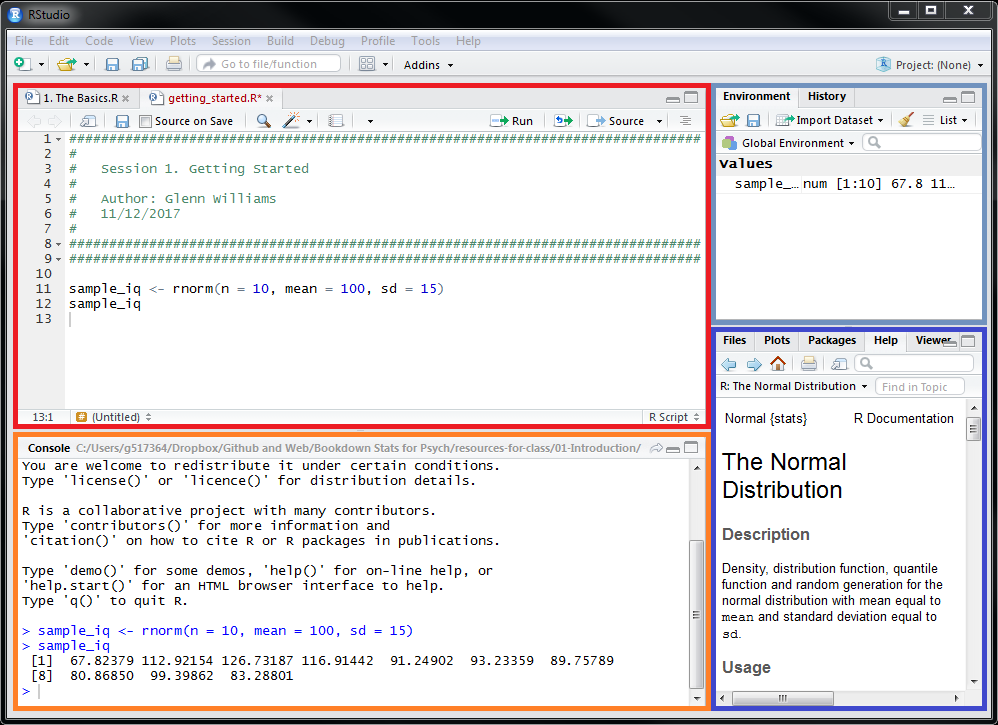
\includegraphics[width=13.86in]{img/r_studio} \end{center}

RStudio can be split into 4 main panes:

\begin{enumerate}
\def\labelenumi{\arabic{enumi}.}
\tightlist
\item
  The {\textbf{editor}}: Type, edit, and save scripts as you would in any text editor.
\item
  The {\textbf{console}}: Execute scripts by typing and pressing enter.
\item
  The {\textbf{environment and history}}: View objects (e.g.~values, variables, and user-defined functions etc.) stored in memory for this working session. You can also see a history of your commands in the \emph{History} tab.
\item
  The {\textbf{viewer}}: view any \emph{files} in your working directory, see your last \emph{plot} from this session, view installed \emph{packages} on your machine (you can also load them here), view the \emph{help} documentation for any R commands, in the \emph{viewer} you can view (surprise, surprise) markdown/other documents.
\end{enumerate}

All of these panes are very useful when developing your R scripts, but RStudio has some other features such as syntax highlighting, code completion, and an easy interface for compiling your reproducible R-markdown notebooks. For advanced users, you can also set up projects that play nicely with \href{https://github.com/}{Github} for version control of your work.

Finally, RStudio defaults to giving you the option to save your workspace (e.g.~all of the data you've created) when you close the program and to restore this workspace once you restart RStudio. I'd advise you to change RStudio's defaults to never do this as this could cause unforseen errors when, for example, you want to change parts of script and you accidentally delete the stage to create a variable that is crucial later on. This deletion may not be obvious if you reload your workspace, but you won't have a record of how you created said variable. To make these changes, go to \textbf{Tools, Global Options} then deselect \textbf{Restore .RData into workspace at startup} and from the dropdown menu on \textbf{Save workspace to .RData on exit:} to \textbf{Never}.

\hypertarget{working-directory-and-file-paths}{%
\section{Working Directory and File Paths}\label{working-directory-and-file-paths}}

When you create an R file (File, New File, R Script), where that file sits is its \textbf{working directory}. This is where R interprets any commands that go outside of your R session. For example, if you want to read data into R, or output a graph, R will do so in respect to the working directory. You can \emph{get} your \emph{working directory} like so:

\begin{Shaded}
\begin{Highlighting}[]
\FunctionTok{getwd}\NormalTok{()}
\end{Highlighting}
\end{Shaded}

You should see something along the lines of ``C:/Users/\emph{YOUR\_NAME}/FOLDER/\emph{RFILE}.R''

Now, you can set your working directory to any folder on your computer with an absolute file path. Often, people use absolute file paths in order read inputs and send outputs to different folders on their computer, telling R exactly where to look.

However, I recommend against this. That's because if you change computers or pass your code over to someone else R will kick out an error saying it can't find that folder; other computers are highly unlikely to have the same folder structure or even username as you, and fixing this can be frustrating. Also, it can be a pain having to type out your full file path, so let's avoid that. Below, I've outlined one method for working that will allow you to use relative filepaths (relatively) easily.

If you want to keep your folder from getting cluttered, keep your R script(s) in a folder, with an Inputs and Outputs folder at that same level, like so:

Potential Folder Structure for Your Projects

This way, when you want to read in raw data, or output a graph (or something else) you can use a \textbf{relative file path} rather than an absolute file path to define where your files are taken from/should go. This saves you a lot of typing of file paths, and it means your R scripts will work on someone else's computer if you just send the entire folder containing the R script, Inputs, and Outputs folders.

To read in or save data using a relative file path, do this:

\begin{Shaded}
\begin{Highlighting}[]
\CommentTok{\# reads a CSV file from the Inputs folder}
\NormalTok{my\_data }\OtherTok{\textless{}{-}} \FunctionTok{read.csv}\NormalTok{(}\StringTok{"Inputs/my\_data.csv"}\NormalTok{) }

\CommentTok{\# writes a CSV file to the Outputs folder}
\NormalTok{my\_data }\OtherTok{\textless{}{-}} \FunctionTok{write.csv}\NormalTok{(my\_data, }\StringTok{"Outputs/my\_data\_again.csv"}\NormalTok{) }
\end{Highlighting}
\end{Shaded}

You just have to type in the folder name and a slash (to indicate to go below that folder) and the name of your data. This saves you from all of the hassle of using an abosolute file path described above.

\hypertarget{packages}{%
\section{Packages}\label{packages}}

Next, while you can do a lot in base R, if you can think of some task that is reasonably laborious there's probably a package out there that can help you to achieve a certain goal. For us, the whole data processing, analysis, and presentation workflow can be made so much simpler by using a set of packages from the tidyverse library \citep{R-tidyverse}. This package is required for what we're about to do next, so install tidyverse (using \texttt{install.packages("tidyverse")}). Once installed, you needn't do it again. But on each new session you have to define which packages you want to load into R using the \texttt{library()} command. Make sure to uncomment the \texttt{install.packages("tidyverse")} line if you haven't installed this package yet.

\begin{Shaded}
\begin{Highlighting}[]
\CommentTok{\# install.packages("tidyverse") \# do this only once to install the package}
\FunctionTok{library}\NormalTok{(tidyverse) }\CommentTok{\# do this to load your package every time you open R}
\end{Highlighting}
\end{Shaded}

\begin{verbatim}
## -- Attaching packages ------------------- tidyverse 1.3.2 --
## v ggplot2 3.3.6      v purrr   0.3.4 
## v tibble  3.1.8      v dplyr   1.0.10
## v tidyr   1.2.1      v stringr 1.4.1 
## v readr   2.1.2      v forcats 0.5.2 
## -- Conflicts ---------------------- tidyverse_conflicts() --
## x dplyr::filter() masks stats::filter()
## x dplyr::lag()    masks stats::lag()
\end{verbatim}

By default, R installs packages from CRAN, which is essentially a centralised network for all things R. However, some useful packages may not have been submitted here, and you can install them from other places, like \href{https://github.com/}{GitHub}. We won't install packages from github or other repositories in this course. But it's worth knowing that you can install packages from just about anywhere!

Most of the time, you won't have any trouble using functions from a loaded package. However, there can be cases when you have two packages installed that use the same function name. To tell R exactly which version of a function to use, we can specify both the package and function name in the form \texttt{package::function\_name()}. For example, we can use the \texttt{group\_by()} function from the package \texttt{dplyr} by typing \texttt{dplyr::group\_by()}. You won't come across this in this course, as we'll be using packages that have functions with unique names, but it's worth bearing in mind if you come across problems with functions you \emph{know} should work in the future.

\emph{Note}: You may notice that in my code chunks I have some green text following a \#. These are comments in R and are not read when you execute your code. Comments are very useful for telling you what each section of your code does, and how. I tend to comment quite heavily, as there's always a chance you'll forget what you've done when you go back to it after a few months away from the code.

\hypertarget{objects-and-functions}{%
\section{Objects and Functions}\label{objects-and-functions}}

You can use R like a calculator, e.g.

\begin{Shaded}
\begin{Highlighting}[]
\DecValTok{1} \SpecialCharTok{+} \DecValTok{4}
\end{Highlighting}
\end{Shaded}

\begin{verbatim}
## [1] 5
\end{verbatim}

You can execute this directly in the console, or run it from your R script by selecting that line of code (or highlighting several lines) and pressing Ctrl + Enter (for mac, this is probably Cmd + Enter). While I said you shouldn't use the console when writing scripts, you can use it to test out a bit of code, or to quickly use R as a calculator when you're in a meeting and feeling like mental arithmetic is a step too far. You can see that once the code is run, the R console returns the result back to you. You see a history of what you asked, and what was returned.

\emph{Top tip}: use the up arrow key from the console and R will automatically fill in the last line/block of code you ran. Press up again to cycle back to older inputs, and down to back to the most recent ones.

R always waits for you to finish an expression before it runs your code. So, if you ended your line with a +, it'll wait for the next number. This is useful for complex expressions that can take up multiple lines, e.g.

\begin{Shaded}
\begin{Highlighting}[]
\DecValTok{1} \SpecialCharTok{+} \DecValTok{2} \SpecialCharTok{+} \DecValTok{3} \SpecialCharTok{+} \DecValTok{4} \SpecialCharTok{+} \DecValTok{5} \SpecialCharTok{+} \DecValTok{6} \SpecialCharTok{+} \DecValTok{7} \SpecialCharTok{+}
  \DecValTok{8} \SpecialCharTok{+} \DecValTok{9}
\end{Highlighting}
\end{Shaded}

\begin{verbatim}
## [1] 45
\end{verbatim}

Watch the console when you type this out. You'll notice that if you press enter after typing \texttt{7\ +} on the new line you will no longer see \texttt{\textgreater{}} but you'll see +. The same happens even if you pass a different mathematical operator (e.g.~\texttt{-}, \texttt{\%}, \texttt{\^{}}). This is there to tell you that R is not waiting for a new statement, but is waiting for you to finish off the current statement. If you see \texttt{\textgreater{}} it means that whatever you can start a new statement.

R also parses text if included in quotes. The same rule applies about finishing expressions here; if you don't close your quote, then R will wait for you to do so. This means you can spread your text over several lines (by pressing Enter) and R will parse that as one expression. Note with our output we get \textbackslash n which indicates that a new line follows the comma.

\begin{Shaded}
\begin{Highlighting}[]
\StringTok{"Hello, world!"}
\end{Highlighting}
\end{Shaded}

\begin{verbatim}
## [1] "Hello, world!"
\end{verbatim}

\begin{Shaded}
\begin{Highlighting}[]
\StringTok{"How are you doing today? }
\StringTok{Things certainly have been interesting these past few years."}
\end{Highlighting}
\end{Shaded}

\begin{verbatim}
## [1] "How are you doing today? \nThings certainly have been interesting these past few years."
\end{verbatim}

Crucially, you can store this sort of information in a variable. Variables are useful because you may want to use the results of a calculation and do some further operations on that result. This is especially useful if you're not sure what that first result could be. We assign values to a variable using the assignment operator \texttt{\textless{}-} (read this as create from).

\begin{Shaded}
\begin{Highlighting}[]
\NormalTok{summed\_numbers }\OtherTok{\textless{}{-}} \DecValTok{5} \SpecialCharTok{+} \DecValTok{8}
\end{Highlighting}
\end{Shaded}

We can then output this variable later on, like so: (This is often useful for checking that your variables store what you think they store.)

\begin{Shaded}
\begin{Highlighting}[]
\NormalTok{summed\_numbers}
\end{Highlighting}
\end{Shaded}

\begin{verbatim}
## [1] 13
\end{verbatim}

Or we can perform operations on the variable.

\begin{Shaded}
\begin{Highlighting}[]
\NormalTok{summed\_numbers}\SpecialCharTok{*}\DecValTok{5}
\end{Highlighting}
\end{Shaded}

\begin{verbatim}
## [1] 65
\end{verbatim}

\emph{Note}: You cannot start variables with a number, you cannot use special characters (e.g.~\%!*) and you cannot include spaces in your variable name. Also, note that your capitalisation matters, so Summed\_numbers is not summed\_numbers. (I often get errors due to this issue\ldots)

R has the simple arithmetic operations you'd expect from any program. For example, you can:

\begin{itemize}
\tightlist
\item
  add \texttt{x\ +\ y},
\item
  subtract \texttt{x\ -\ y},
\item
  multiply \texttt{x\ *\ y}
\item
  divide \texttt{x/y},
\item
  exponentiate \texttt{x\^{}y}
\item
  find the modulus \texttt{x\ \%\%\ y}, (e.g.~5 mod 2 = 1; i.e.~the remainder from how many times 2 goes into 5)
\item
  and conduct integer division \texttt{x\ \%/\%\ y} (e.g.~5 int div 2 = 2)
\end{itemize}

R also has some logical operations built in. For example:

\begin{itemize}
\tightlist
\item
  less than \texttt{x\ \textless{}\ y}
\item
  less than or equal to \texttt{x\ \textless{}=\ y}
\item
  greater than \texttt{x\ \textgreater{}\ y}
\item
  greater than or equal to \texttt{x\ \textgreater{}=\ y}
\item
  exactly equal to \texttt{x\ ==\ y}
\item
  not equal to \texttt{x\ !=\ y}
\item
  not x \texttt{!x}
\item
  x OR y \texttt{x\ \textbar{}\ y}
\item
  x AND y \texttt{x\ \&\ y}
\item
  test if X is true \texttt{isTRUE(x)}
\end{itemize}

These come in pretty handy for performing most operations on our data. If you're unfamiliar with these, don't worry. We'll cover how you might use some of these in a staggered format as you progress through this course. Nicely, R also has a number of functions built in. This means you don't need to write your own function if you want to sum a sequence of numbers. I'm sure I couldn't provide an exhaustive list here, but as stated above we'll cover most of the common functions as you get to grips with some data. Still, lets get an idea of how these functions work.

Below, we will sum the numbers 1 to 4. This function is built into R already, so we don't have to write a whole lot of code for this.

\begin{Shaded}
\begin{Highlighting}[]
\FunctionTok{sum}\NormalTok{(}\DecValTok{1}\NormalTok{, }\DecValTok{2}\NormalTok{, }\DecValTok{3}\NormalTok{, }\DecValTok{4}\NormalTok{)}
\end{Highlighting}
\end{Shaded}

\begin{verbatim}
## [1] 10
\end{verbatim}

What if we want to calculate the mean score from this set of numbers? That's also built into R.

\begin{Shaded}
\begin{Highlighting}[]
\FunctionTok{mean}\NormalTok{(}\DecValTok{1}\NormalTok{, }\DecValTok{2}\NormalTok{, }\DecValTok{3}\NormalTok{, }\DecValTok{4}\NormalTok{)}
\end{Highlighting}
\end{Shaded}

\begin{verbatim}
## [1] 1
\end{verbatim}

Notice that whenever we want to run a function, these functions always have a name and are followed by parentheses (e.g.~\texttt{mean()}, \texttt{sum()}). What goes in the parentheses? The argument you want to pass to the function. These can have default values, or not (requiring you to specify the argument). Above, we passed the values 1 through 4 as the arguments to the \texttt{mean()} function. Later, we'll look at functions that ask for arguments from separate data types (e.g.~numbers and characters). If you're unsure what an argument does, you can always ask R what it does, how it does it, and what to pass to it by using \texttt{?}, e.g.~\texttt{?mean()}. This will bring up a document in the Help window of RStudio.

Typing out all of these numbers each time we want to perform some operation is a little tedious. To fix this, we can use what we learned above and store these numbers into a variable. In order to save these into their own variable, we use the \texttt{c} function. Think of this as \textbf{c}oncatenation. When we combine values into a variable, this variable is stored in our global environment. This means that we can perform operations on the variable later on, without the worry of typing our the values again. This is particularly useful if you want to store values from one function (say a statistical test) that you cannot pre-define but that you want to use later on.

Let's give that a go. First, we'll concatenate our values into a variable using the \texttt{c()} function described above. Here, we simply define that we want to concatenate some values, and list each value separated by a comma.

\begin{Shaded}
\begin{Highlighting}[]
\NormalTok{stored\_values }\OtherTok{\textless{}{-}} \FunctionTok{c}\NormalTok{(}\DecValTok{1}\NormalTok{, }\DecValTok{2}\NormalTok{, }\DecValTok{3}\NormalTok{, }\DecValTok{4}\NormalTok{)}
\end{Highlighting}
\end{Shaded}

If we then call a function that works with a set of numbers, it should also work if we call that function on the variable storing those numbers. Let's see how this works with the \texttt{mean()} function.

\begin{Shaded}
\begin{Highlighting}[]
\FunctionTok{mean}\NormalTok{(stored\_values)}
\end{Highlighting}
\end{Shaded}

\begin{verbatim}
## [1] 2.5
\end{verbatim}

Great! That'll save is a lot of time writing and rewriting code later on. This also allows our code to be flexible, in that we can write a script that performs operations on variables that can take any range of values. This, to me, is one of the nicest things about doing your analyses in R. While you may spend more time getting your script up and running in the first place when compared to using point-and-click methods (e.g.~in SPSS), if you gain new data or run a new experiment, it's likely that your script can simply be re-run with no (or few) changes at very little cost to your time.

Now, this part is pretty important but may only be obvious if you've programmed in other languages. R is a \textbf{vectorised} language, which means that, as with the \texttt{sum()} function above, R can perform operations on the entire variable So, if you want to increment all values in your variable by 1, you can simply tell R to do so in one line of code, without the need for loops or other complex methods.

\begin{Shaded}
\begin{Highlighting}[]
\NormalTok{stored\_values }\SpecialCharTok{+} \DecValTok{1}
\end{Highlighting}
\end{Shaded}

\begin{verbatim}
## [1] 2 3 4 5
\end{verbatim}

\hypertarget{creating-and-accessing-data}{%
\section{Creating and Accessing Data}\label{creating-and-accessing-data}}

So, you've made it through all of the boring stuff. Now we can look at manipulating some data in R.

Let's pretend we've administered IQ tests to 100 participants. For some reason, we're interested in whether dog and cat owners have different IQs. I'm sure some of you can come up with some incredibly biased hypotheses here, but we'll leave that out for now.

We'll create this data in R, then take a look at it using some of the packages from the \texttt{tidyverse} library that you installed and loaded above. If the functions below don't work, be sure to load the tidyverse library (using \texttt{library(tidyverse)}) before running the code below.

First, we'll create a variable containing the numbers 1 to 100, using the \texttt{seq()} function; this can be our participant ID variable. Next, we'll use the \texttt{sample()} function to sample randomly (and with replacement) from the two labels ``cat'' and ``dog'' which acts as our factor for pet ownership. (Note that here I use the \texttt{sample()} function on the concatenated values of ``cat'' and ``dog'', but this would work equally well with a variable containing these labels.) Finally, we'll use the \texttt{rnorm()} function to generate some random numbers (sampled from the normal distribution) with a mean of 150, and a standard deviation of 15 to act as our IQ scores.

Remember how I said we'd look at functions that take several arguments? Well, thats what all of these functions below do. We define each parameter of the argument within the function call. So, if we want to generate a sequence of numbers from 1 to 100 , in increments of 1s (e.g.~\texttt{seq(from\ =\ 1,\ to\ =\ 100,\ by\ =\ 1)}), then we define each argument with its name (e.g.~from/to/by) and tell R which values to set for these arguments using \texttt{=}.

\begin{Shaded}
\begin{Highlighting}[]
\CommentTok{\# create participant IDs}
\NormalTok{participant }\OtherTok{\textless{}{-}} \FunctionTok{seq}\NormalTok{(}\AttributeTok{from =} \DecValTok{1}\NormalTok{, }\AttributeTok{to =} \DecValTok{100}\NormalTok{, }\AttributeTok{by =} \DecValTok{1}\NormalTok{)}

\CommentTok{\# create pet ownership codes}
\FunctionTok{set.seed}\NormalTok{(}\DecValTok{88}\NormalTok{)}
\NormalTok{pet }\OtherTok{\textless{}{-}} \FunctionTok{sample}\NormalTok{(}\FunctionTok{c}\NormalTok{(}\StringTok{"cat"}\NormalTok{, }\StringTok{"dog"}\NormalTok{), }\DecValTok{100}\NormalTok{, }\AttributeTok{replace =} \ConstantTok{TRUE}\NormalTok{)}

\CommentTok{\# create IQ scores}
\FunctionTok{set.seed}\NormalTok{(}\DecValTok{88}\NormalTok{)}
\NormalTok{IQ\_score }\OtherTok{\textless{}{-}} \FunctionTok{rnorm}\NormalTok{(}\AttributeTok{n =} \DecValTok{100}\NormalTok{, }\AttributeTok{mean =} \DecValTok{150}\NormalTok{, }\AttributeTok{sd =} \DecValTok{15}\NormalTok{)}
\NormalTok{IQ\_score }\OtherTok{\textless{}{-}} \FunctionTok{round}\NormalTok{(IQ\_score) }\CommentTok{\# round IQ scores}
\end{Highlighting}
\end{Shaded}

\emph{Note:} I've overspecified the functions above. You can simply run \texttt{seq(1:\ 100)} and \texttt{rnorm(100,\ 150,\ 15)} to get the same results, but it's a little less readable. Here, and throughout, I'll use the most readable version so you have the best idea of what you're doing. Because we're using random sampling, I've also set a seed, so that you'll sample the same values as me. If you want people to be able to reproduce your random sampling so they get the same data, set a seed!

Finally, it's important to note that you can call a function on the result of another function in R.

Right now, each number in the participant variable is unique. We can see how many participants are in the study by asking R ``how long is the variable, participant?''. We do this like so:

\begin{Shaded}
\begin{Highlighting}[]
\FunctionTok{length}\NormalTok{(participant)}
\end{Highlighting}
\end{Shaded}

\begin{verbatim}
## [1] 100
\end{verbatim}

Cool, we have 100 participants! But what if we have several observations for one participant? I'll define that (very simply) in the code below:

\begin{Shaded}
\begin{Highlighting}[]
\NormalTok{participant[}\DecValTok{2}\NormalTok{] }\OtherTok{\textless{}{-}} \DecValTok{1} \CommentTok{\# assign the second value of participant the integer 1}
\FunctionTok{head}\NormalTok{(participant) }\CommentTok{\# return the first 6 values of the participant variable}
\end{Highlighting}
\end{Shaded}

\begin{verbatim}
## [1] 1 1 3 4 5 6
\end{verbatim}

Now, using \texttt{length(participant)} will return 100, because there's still 100 values in the \texttt{participant} variable. How do we find how many \textbf{unique} numbers are in the \texttt{participant} variable? We simply nest the \texttt{unique()} function within the \texttt{length()} function:

\begin{Shaded}
\begin{Highlighting}[]
\FunctionTok{length}\NormalTok{(}\FunctionTok{unique}\NormalTok{(participant))}
\end{Highlighting}
\end{Shaded}

\begin{verbatim}
## [1] 99
\end{verbatim}

This asks R how many unique values are in the variable participant. That's 99!

\hypertarget{data-frames-and-tibbles}{%
\subsubsection{Data Frames and Tibbles}\label{data-frames-and-tibbles}}

Now, in the real world, if you tested IQs you'd typically have this data stored in a table somewhere prior to reading it into R. So lets pair the data together into a table in R. The most useful way to do this is to create a \texttt{data.frame}. But, since we've already loaded the tidyverse, we may as well use the built in \textbf{tibbles}. These are like data frames, but they have some different defaults that make working in the tidyverse easier.

\begin{Shaded}
\begin{Highlighting}[]
\NormalTok{IQ\_data }\OtherTok{\textless{}{-}}\NormalTok{ tibble}\SpecialCharTok{::}\FunctionTok{tibble}\NormalTok{(}
  \AttributeTok{participant\_number =}\NormalTok{ participant, }
  \AttributeTok{pet\_id =}\NormalTok{ pet, }
  \AttributeTok{IQ =}\NormalTok{ IQ\_score}
\NormalTok{  )}
\end{Highlighting}
\end{Shaded}

What's the main advantage of using a tibble over a \texttt{data.frame} here? Tibbles don't automatically convert certain data types. With \texttt{data.frame}, character data is automatically converted to a factor. This can be useful, but not always. The thing I like most is that tibbles show the data type under the column name. This is taken from \texttt{str()} which tells you the \textbf{str}ucture of your data. Also, tibbles default to printing the first 10 rows of data when you type their name in the console. This will stop you from getting overwhelmed by a massive printout if you have a lot of data. Let's see all of this in action.

\begin{Shaded}
\begin{Highlighting}[]
\NormalTok{IQ\_data}
\end{Highlighting}
\end{Shaded}

\begin{verbatim}
## # A tibble: 100 x 3
##    participant_number pet_id    IQ
##                 <dbl> <chr>  <dbl>
##  1                  1 cat      147
##  2                  1 cat      160
##  3                  3 dog      185
##  4                  4 cat      122
##  5                  5 cat      157
##  6                  6 dog      152
##  7                  7 cat      152
##  8                  8 cat      119
##  9                  9 cat      131
## 10                 10 dog      160
## # ... with 90 more rows
\end{verbatim}

If you want more than 10 rows, or a specific number of columns, tell R that's what you'd like. Here, we've asked for the first 12 rows, and the width of the table to be infinity so that R prints out all columns even if they don't fit on 1 row in the console. However, with only 3 columns, that isn't an issue here.

\begin{Shaded}
\begin{Highlighting}[]
\FunctionTok{print}\NormalTok{(IQ\_data, }\AttributeTok{n =} \DecValTok{12}\NormalTok{, }\AttributeTok{width =} \ConstantTok{Inf}\NormalTok{)}
\end{Highlighting}
\end{Shaded}

\begin{verbatim}
## # A tibble: 100 x 3
##    participant_number pet_id    IQ
##                 <dbl> <chr>  <dbl>
##  1                  1 cat      147
##  2                  1 cat      160
##  3                  3 dog      185
##  4                  4 cat      122
##  5                  5 cat      157
##  6                  6 dog      152
##  7                  7 cat      152
##  8                  8 cat      119
##  9                  9 cat      131
## 10                 10 dog      160
## 11                 11 cat      138
## 12                 12 dog      165
## # ... with 88 more rows
\end{verbatim}

Unfortunately, some older functions in R won't allow you to use a tibble. If this is the case, simply convert your tibble to a \texttt{data.frame} using the \texttt{as.data.frame()} function. Note, we use \texttt{head()} to see the head of our data frame, or the first 6 values. This is necessary here to avoid printing out each row, as we're not in using a tibble any more. Notice that We've assigned the \texttt{data.frame} version of our IQ data to a new variable, rather than overwriting the previous variable. This is good practice when testing your code, as you never know what might break, resulting in data loss. (Although this wansn't strictly necessary here.)

\begin{Shaded}
\begin{Highlighting}[]
\NormalTok{IQ\_data\_df }\OtherTok{\textless{}{-}} \FunctionTok{as.data.frame}\NormalTok{(IQ\_data)}
\FunctionTok{head}\NormalTok{(IQ\_data\_df)}
\end{Highlighting}
\end{Shaded}

\begin{verbatim}
##   participant_number pet_id  IQ
## 1                  1    cat 147
## 2                  1    cat 160
## 3                  3    dog 185
## 4                  4    cat 122
## 5                  5    cat 157
## 6                  6    dog 152
\end{verbatim}

\hypertarget{accessing-tibble-information}{%
\subsubsection{Accessing Tibble Information}\label{accessing-tibble-information}}

With tibbles and \texttt{data.frames}, you often want to access a specific column in order to perform some calculation. Let's say we want to calculate the mean IQ score in our data set. Why doesn't the code below work?

\begin{Shaded}
\begin{Highlighting}[]
\FunctionTok{mean}\NormalTok{(IQ\_data)}
\end{Highlighting}
\end{Shaded}

\begin{verbatim}
## Warning in mean.default(IQ_data): argument is not numeric or logical: returning
## NA
\end{verbatim}

\begin{verbatim}
## [1] NA
\end{verbatim}

R gives us a warning, saying that the argument to our function (i.e.~the tibble, IQ\_data) is not numeric or logical. Therefore, R cannot calculate the mean on something that isn't a number (or set of numbers). Instead, we have to point R to the correct column within the tibble. This is often done by name using \texttt{\$} , or by name/position in the tibble using \texttt{{[}{[}} and the name/position followed by \texttt{{]}{]}}.

First, let's see that we're accessing everything correctly here.

\begin{Shaded}
\begin{Highlighting}[]
\CommentTok{\# by name}
\NormalTok{IQ\_data}\SpecialCharTok{$}\NormalTok{IQ}
\NormalTok{IQ\_data[[}\StringTok{"IQ"}\NormalTok{]]}

\CommentTok{\# by position}
\NormalTok{IQ\_data[[}\DecValTok{3}\NormalTok{]]}
\end{Highlighting}
\end{Shaded}

\begin{verbatim}
## [1] 147 160 185 122 157 152
\end{verbatim}

Tibbles are stricter than data frames, in that they'll always return a tibble. For example, with a \texttt{data.frame} if you ask for a value in a specific row of a specific column under the format \texttt{data\_frame{[}row,\ column{]}}, R will return a vector of the value at that position in the \texttt{data.frame}. With tibbles, your single value will be returned as a tibble.

\begin{Shaded}
\begin{Highlighting}[]
\CommentTok{\# tibble output}
\NormalTok{IQ\_data[}\DecValTok{1}\NormalTok{, }\DecValTok{3}\NormalTok{] }\CommentTok{\# row 1, col 3}
\end{Highlighting}
\end{Shaded}

\begin{verbatim}
## # A tibble: 1 x 1
##      IQ
##   <dbl>
## 1   147
\end{verbatim}

\begin{Shaded}
\begin{Highlighting}[]
\CommentTok{\# data.frame output}
\NormalTok{IQ\_data\_df[}\DecValTok{1}\NormalTok{, }\DecValTok{3}\NormalTok{]}
\end{Highlighting}
\end{Shaded}

\begin{verbatim}
## [1] 147
\end{verbatim}

Now, lets calculate the mean on the correct column in the tibble. Personally, I prefer using \texttt{\$} for cases like this. But, feel free to use any of the above methods.

\begin{Shaded}
\begin{Highlighting}[]
\FunctionTok{mean}\NormalTok{(IQ\_data}\SpecialCharTok{$}\NormalTok{IQ)}
\end{Highlighting}
\end{Shaded}

\begin{verbatim}
## [1] 150.17
\end{verbatim}

We can combine what we learned above about \texttt{c()} to access multiple columns at once:

\begin{Shaded}
\begin{Highlighting}[]
\NormalTok{IQ\_data[, }\FunctionTok{c}\NormalTok{(}\StringTok{"participant\_number"}\NormalTok{, }\StringTok{"IQ"}\NormalTok{)]}
\end{Highlighting}
\end{Shaded}

\begin{verbatim}
## # A tibble: 100 x 2
##    participant_number    IQ
##                 <dbl> <dbl>
##  1                  1   147
##  2                  1   160
##  3                  3   185
##  4                  4   122
##  5                  5   157
##  6                  6   152
##  7                  7   152
##  8                  8   119
##  9                  9   131
## 10                 10   160
## # ... with 90 more rows
\end{verbatim}

Or we can access a range of values by specifying the rows we'd like to access:

\begin{Shaded}
\begin{Highlighting}[]
\NormalTok{IQ\_data[}\FunctionTok{c}\NormalTok{(}\DecValTok{1}\NormalTok{, }\DecValTok{2}\NormalTok{, }\DecValTok{3}\NormalTok{, }\DecValTok{4}\NormalTok{, }\DecValTok{5}\NormalTok{), }\FunctionTok{c}\NormalTok{(}\StringTok{"participant\_number"}\NormalTok{, }\StringTok{"IQ"}\NormalTok{)]}
\end{Highlighting}
\end{Shaded}

\begin{verbatim}
## # A tibble: 5 x 2
##   participant_number    IQ
##                <dbl> <dbl>
## 1                  1   147
## 2                  1   160
## 3                  3   185
## 4                  4   122
## 5                  5   157
\end{verbatim}

or, to save typing, we can just define this from a starting to an ending value for the rows:

\begin{Shaded}
\begin{Highlighting}[]
\NormalTok{IQ\_data[}\DecValTok{1}\SpecialCharTok{:}\DecValTok{5}\NormalTok{, }\FunctionTok{c}\NormalTok{(}\StringTok{"participant\_number"}\NormalTok{, }\StringTok{"IQ"}\NormalTok{)]}
\end{Highlighting}
\end{Shaded}

\begin{verbatim}
## # A tibble: 5 x 2
##   participant_number    IQ
##                <dbl> <dbl>
## 1                  1   147
## 2                  1   160
## 3                  3   185
## 4                  4   122
## 5                  5   157
\end{verbatim}

In \textbf{Session 4} we'll look at more intuitive ways of accessing data from columns and rows in your data frames. However, for now we'll quickly look at ways to manipulate data using the base R functionality so you have some idea how indexing works in R.

\hypertarget{manipulating-tibble-information}{%
\subsubsection{Manipulating Tibble Information}\label{manipulating-tibble-information}}

\hypertarget{changing-values}{%
\paragraph{Changing Values}\label{changing-values}}

We can use these same principles to edit the information within our data. Say, we'd like to change participant number in row 2 back to 2, we just need to do this:

\begin{Shaded}
\begin{Highlighting}[]
\CommentTok{\# specifying row and column by index}
\NormalTok{IQ\_data[}\DecValTok{2}\NormalTok{, }\DecValTok{1}\NormalTok{] }\OtherTok{\textless{}{-}} \DecValTok{2}

\CommentTok{\# specifying row by index and column by name}
\NormalTok{IQ\_data[}\DecValTok{2}\NormalTok{, }\StringTok{"participant\_number"}\NormalTok{] }\OtherTok{\textless{}{-}} \DecValTok{2}

\CommentTok{\# specifying index within a column}
\NormalTok{IQ\_data}\SpecialCharTok{$}\NormalTok{participant\_number[}\DecValTok{2}\NormalTok{] }\OtherTok{\textless{}{-}} \DecValTok{2}
\end{Highlighting}
\end{Shaded}

You can see how all of this combined can result in some pretty powerful flexibility in how you access and manipulate your data in R.

\hypertarget{adding-and-removing-columns}{%
\paragraph{Adding and Removing Columns}\label{adding-and-removing-columns}}

To add a row to a data frame, we simply need to specify what we want to add and assign it a new name. Let's say that we want to add a column that indicates the operating system used by each participant.

We may have this because we made assumptions that people who use Windows, macOS, or the Linux families of operating systems differ in their IQ. This is a silly example for several reasons, not only because you can use more than one system; but we'll stick with this for now.

Imagine we already have a sample of operating systems to draw from. You don't need to understand how this works, but briefly I've used the inbuilt \texttt{sample()} function to pick from the three names with replacement, skewing the probabilities to select windows most often, followed by mac, then linux. All that matters is that we're assigning 100 names to a variable.

\begin{Shaded}
\begin{Highlighting}[]
\FunctionTok{set.seed}\NormalTok{(}\DecValTok{1000}\NormalTok{) }\CommentTok{\# make the sampling procedure the same for us all}

\NormalTok{operating\_system }\OtherTok{\textless{}{-}} \FunctionTok{sample}\NormalTok{(}\FunctionTok{c}\NormalTok{(}\StringTok{"windows"}\NormalTok{, }\StringTok{"mac"}\NormalTok{, }\StringTok{"linux"}\NormalTok{), }
                           \AttributeTok{size =} \DecValTok{100}\NormalTok{, }
                           \AttributeTok{replace =} \ConstantTok{TRUE}\NormalTok{,}
                           \AttributeTok{prob =} \FunctionTok{c}\NormalTok{(}\FloatTok{0.5}\NormalTok{, }\FloatTok{0.3}\NormalTok{, }\FloatTok{0.2}\NormalTok{)}
\NormalTok{                           )}
\end{Highlighting}
\end{Shaded}

In the \texttt{IQ\_data} set, we can add a new column for the operating systems used by the participants like so:

\begin{Shaded}
\begin{Highlighting}[]
\NormalTok{IQ\_data}\SpecialCharTok{$}\NormalTok{operating\_system }\OtherTok{\textless{}{-}}\NormalTok{ operating\_system }\CommentTok{\# add new column}

\FunctionTok{head}\NormalTok{(IQ\_data) }\CommentTok{\# view first 6 rows}
\end{Highlighting}
\end{Shaded}

\begin{verbatim}
## # A tibble: 6 x 4
##   participant_number pet_id    IQ operating_system
##                <dbl> <chr>  <dbl> <chr>           
## 1                  1 cat      147 windows         
## 2                  2 cat      160 mac             
## 3                  3 dog      185 windows         
## 4                  4 cat      122 mac             
## 5                  5 cat      157 mac             
## 6                  6 dog      152 windows
\end{verbatim}

Note that you can rename the column to anything you like. But, for consistency, I like to keep the same name as the variable which acts as the data source.

Finally, we can remove the new column (and any column) by setting the entire column to nothing (\texttt{NULL}), like so:

\begin{Shaded}
\begin{Highlighting}[]
\NormalTok{IQ\_data}\SpecialCharTok{$}\NormalTok{operating\_system }\OtherTok{\textless{}{-}} \ConstantTok{NULL} \CommentTok{\# remove new column}

\FunctionTok{head}\NormalTok{(IQ\_data) }\CommentTok{\# view first 6 rows}
\end{Highlighting}
\end{Shaded}

\begin{verbatim}
## # A tibble: 6 x 3
##   participant_number pet_id    IQ
##                <dbl> <chr>  <dbl>
## 1                  1 cat      147
## 2                  2 cat      160
## 3                  3 dog      185
## 4                  4 cat      122
## 5                  5 cat      157
## 6                  6 dog      152
\end{verbatim}

Now the data is back to its original format.

We'll look at another way to remove one or several columns from your data frame in \textbf{Session 4}, but for now this a quick way to get things done using base R.

\hypertarget{adding-and-removing-rows}{%
\paragraph{Adding and Removing Rows}\label{adding-and-removing-rows}}

What if we want to add a new row to our data? This may be less common than adding a new column for data processing purposes, but it's good to know anyway.

First, we need to know what should go in each cell. Remember that we have to keep the data square, so you can't have missing values when you add a row. If you don't have any data, you can just put \texttt{NA} (with \textbf{no quotations}) to keep the data square but to show that you don't have any value for a given cell.

Let's assume we want to add a new participant, 101, who has a dog but an unknown IQ. We must define a list of data where we assign values to the columns that match up with our IQ data column headings. We do this like so:

\begin{Shaded}
\begin{Highlighting}[]
\CommentTok{\# add new row with values}
\NormalTok{IQ\_data[}\DecValTok{101}\NormalTok{, ] }\OtherTok{\textless{}{-}} \FunctionTok{list}\NormalTok{(}\AttributeTok{participant\_number =} \DecValTok{101}\NormalTok{, }\AttributeTok{pet\_id =} \StringTok{"dog"}\NormalTok{, }\AttributeTok{IQ =} \ConstantTok{NA}\NormalTok{) }

\FunctionTok{tail}\NormalTok{(IQ\_data) }\CommentTok{\# see last 6 rows}
\end{Highlighting}
\end{Shaded}

\begin{verbatim}
## # A tibble: 6 x 3
##   participant_number pet_id    IQ
##                <dbl> <chr>  <dbl>
## 1                 96 dog      148
## 2                 97 dog      178
## 3                 98 cat      156
## 4                 99 dog      165
## 5                100 cat      150
## 6                101 dog       NA
\end{verbatim}

Here, we have to define all our values to be added in parentheses, using the \texttt{list()} function:

\begin{itemize}
\tightlist
\item
  participant number is \texttt{101}
\item
  pet\_id is \texttt{"dog"}
\item
  IQ is \texttt{NA} (i.e.~unknown)
\end{itemize}

We then assign this to our data frame using the assignment operator (\texttt{\textless{}-}).

We have to tell R where these values should go in our data frame. Because we're adding a new row, we specify the data frame, with row 101, and all columns (remember, an empty value after the comma = all columns).

Note, this is a little more complicated than assigning a new row to our data in a data.frame, but makes us be more specific about what we are adding and where. For more details on lists, keep reading this section.

We can then remove this row again setting our data frame to itself, minus the 101st row:

\begin{Shaded}
\begin{Highlighting}[]
\NormalTok{IQ\_data }\OtherTok{\textless{}{-}}\NormalTok{ IQ\_data[}\SpecialCharTok{{-}}\DecValTok{101}\NormalTok{, ] }\CommentTok{\# remove the new row}

\FunctionTok{tail}\NormalTok{(IQ\_data) }\CommentTok{\# see last 6 rows}
\end{Highlighting}
\end{Shaded}

\begin{verbatim}
## # A tibble: 6 x 3
##   participant_number pet_id    IQ
##                <dbl> <chr>  <dbl>
## 1                 95 dog      188
## 2                 96 dog      148
## 3                 97 dog      178
## 4                 98 cat      156
## 5                 99 dog      165
## 6                100 cat      150
\end{verbatim}

This is a pain as it isn't consistent with removing the rows. But, in \textbf{Session 4} we'll look at removing rows in a consistent way to removing columns. Still, it's useful to know how this process works.

\hypertarget{other-data-types}{%
\subsubsection{Other Data Types}\label{other-data-types}}

For most purposes, you'll only need vectors and data frames/tibbles when you want to work with your data. But it's worth being aware of other data types, such as lists and matrices.

With lists, you can define a vector that contains other objects. Think of this as nesting vectors within vectors (very meta).

\begin{Shaded}
\begin{Highlighting}[]
\NormalTok{person\_quality }\OtherTok{\textless{}{-}} \FunctionTok{list}\NormalTok{(}\AttributeTok{glenn =} \FunctionTok{c}\NormalTok{(}\StringTok{"handsome"}\NormalTok{, }\StringTok{"smart"}\NormalTok{, }\StringTok{"modest"}\NormalTok{),}
                       \AttributeTok{not\_glenn =} \FunctionTok{c}\NormalTok{(}\StringTok{"less\_handsome"}\NormalTok{, }\StringTok{"less\_smart"}\NormalTok{, }\StringTok{"less\_modest"}\NormalTok{)}
\NormalTok{                       )}
\end{Highlighting}
\end{Shaded}

We can then access the elements of a list similarly to how we access vectors, but the name associated with the list will also be returned:

\begin{Shaded}
\begin{Highlighting}[]
\NormalTok{person\_quality[}\DecValTok{1}\NormalTok{]}
\end{Highlighting}
\end{Shaded}

\begin{verbatim}
## $glenn
## [1] "handsome" "smart"    "modest"
\end{verbatim}

If, instead, we just want the values associated with that entry, we can use \texttt{{[}{[}your\ list\ name{]}{]}}:

\begin{Shaded}
\begin{Highlighting}[]
\NormalTok{person\_quality[[}\DecValTok{1}\NormalTok{]]}
\end{Highlighting}
\end{Shaded}

\begin{verbatim}
## [1] "handsome" "smart"    "modest"
\end{verbatim}

We can edit these values in a similar way to how we did with a data frame. This time, we just need to tell R which vector to access first (here, it's the first vector, using double brackets so we can access the values stored there, and not the name (as would happen if we just had 1 bracket)), and then specify which location in the vector you'd like to assign a new value using a separate bracket here:

\begin{Shaded}
\begin{Highlighting}[]
\NormalTok{person\_quality[[}\DecValTok{1}\NormalTok{]][}\DecValTok{4}\NormalTok{] }\OtherTok{\textless{}{-}} \StringTok{"liar"}
\NormalTok{person\_quality[}\DecValTok{1}\NormalTok{]}
\end{Highlighting}
\end{Shaded}

\begin{verbatim}
## $glenn
## [1] "handsome" "smart"    "modest"   "liar"
\end{verbatim}

An advantage to using lists over data frames or tibbles is that the data need not be square. That is, you can have uneven lengths for your entries. Notice how glenn and not\_glenn have different numbers of elements in the list. With a data frame, this is problematic. Let's try adding another participant number to our IQ\_data tibble.

\begin{Shaded}
\begin{Highlighting}[]
\NormalTok{IQ\_data[}\DecValTok{101}\NormalTok{, }\DecValTok{1}\NormalTok{] }\OtherTok{\textless{}{-}} \DecValTok{101}
\FunctionTok{tail}\NormalTok{(IQ\_data)}
\end{Highlighting}
\end{Shaded}

\begin{verbatim}
## # A tibble: 6 x 3
##   participant_number pet_id    IQ
##                <dbl> <chr>  <dbl>
## 1                 96 dog      148
## 2                 97 dog      178
## 3                 98 cat      156
## 4                 99 dog      165
## 5                100 cat      150
## 6                101 <NA>      NA
\end{verbatim}

Did you notice that R automatically introduced NA values in the final cells for the pet\_id and IQ columns?

Matrices work very similarly to data frames and tibbles, but they're even stricter. They can only contain the same data type throughout, so we can't mix columns containing characters and numbers without converting them all to the same data type (hint: it's a character!). I'll show you how to make a matrix, but we won't linger on that as I haven't found them all that useful in my own work.

\begin{Shaded}
\begin{Highlighting}[]
\NormalTok{matrix\_example }\OtherTok{\textless{}{-}} \FunctionTok{matrix}\NormalTok{(}\FunctionTok{rep}\NormalTok{(}\DecValTok{1}\SpecialCharTok{:} \DecValTok{25}\NormalTok{),}
                         \AttributeTok{nrow =} \DecValTok{5}\NormalTok{,}
                         \AttributeTok{ncol =} \DecValTok{5}
\NormalTok{                         )}
\NormalTok{matrix\_example}
\end{Highlighting}
\end{Shaded}

\begin{verbatim}
##      [,1] [,2] [,3] [,4] [,5]
## [1,]    1    6   11   16   21
## [2,]    2    7   12   17   22
## [3,]    3    8   13   18   23
## [4,]    4    9   14   19   24
## [5,]    5   10   15   20   25
\end{verbatim}

\hypertarget{good-practice}{%
\section{Good Practice}\label{good-practice}}

\hypertarget{data-checking-tips}{%
\subsection{Data Checking Tips}\label{data-checking-tips}}

Finally, a few tips on checking your data before you manipulate your data:

\begin{enumerate}
\def\labelenumi{\arabic{enumi}.}
\tightlist
\item
  If you're unsure what you have in your working directory, use either check your environment (the panel in light blue in the RStudio screenshot above) or type \texttt{ls()} in the console. This will list everything currently in the global environment.
\item
  If you want to know the data class for some object, use the \texttt{class()} function (e.g.~\texttt{class(IQ\_data)}).
\item
  If you want to know the structure (including object classes) for some object, use the \texttt{str()} function (e.g.~\texttt{str(IQ\_data)}. Nicely, \texttt{str()} also tells you how many variables are in the object, and how many observations you have in total.
\end{enumerate}

Most importantly with anything in R, if you aren't sure how a function works, or what it's done to your data, check how that function works! You can do this with any function by typing \texttt{?} followed by the function name into the console (e.g.~\texttt{?str()}).

\hypertarget{style}{%
\subsection{Style}\label{style}}

I strongly recommend that you choose a style guide and stick to it throughout when you write your R code. This will make it easier to notice any errors in your code, and increases readability for you and others. Consistency is key here. Since we're using a tidyverse first approach to teaching R in this course, I recommend this one by the creator of the tidyverse:

\href{http://adv-r.had.co.nz/Style.html}{R Style Guide by Hadley Wickham}

The important things to take home are that:

\begin{itemize}
\tightlist
\item
  Use sensible variable names: if a column shows, e.g.~participant weight, call it participant\_weight
\item
  Use verbs to describe user-defined functions: if you write a function to make all the descriptive statistics you could ever want, call it something like make\_descriptives()
\item
  use a consistent style, like snake\_case\_here, or even camelCase, but don't mix\_snake\_and\_camelCase.
\item
  comment your code with descriptions of why you've done something: you can often work out how you did it by following your code, but the why is easily lost!
\end{itemize}

\hypertarget{exercises}{%
\section{Exercises}\label{exercises}}

Try out the exercises below, we'll cover these in the class with the solutions uploaded at the beginning of each session in a separate downloadable link. Try to solve these questions before resorting to the solutions. I'll be there to help out where necessary. First, I want you to figure out why some code doesn't work, then we'll move on to you manipulating data.

For \href{https://youtu.be/yOI8NGJ6SdI}{the opener}, we'll look at the basics of solving issues with your code.

\hypertarget{question-1}{%
\subsection{Question 1}\label{question-1}}

What's wrong with the following code?

\begin{Shaded}
\begin{Highlighting}[]
\CommentTok{\# create a sequence from 0 to 40 in intervals of 2}
\NormalTok{sequence }\SpecialCharTok{\textless{}} \SpecialCharTok{{-}} \FunctionTok{seq}\NormalTok{(}\AttributeTok{from =} \DecValTok{0}\NormalTok{, }\AttributeTok{to =} \DecValTok{40}\NormalTok{, }\AttributeTok{by =} \DecValTok{2}\NormalTok{)}
\end{Highlighting}
\end{Shaded}

\hypertarget{question-2}{%
\subsection{Question 2}\label{question-2}}

Why doesn't this return anything?

\begin{Shaded}
\begin{Highlighting}[]
\CommentTok{\# draw 100 times from a uniform distribution between 1 and 10}
\NormalTok{uniform\_distribution }\OtherTok{\textless{}{-}} \FunctionTok{runif}\NormalTok{(}\AttributeTok{n =} \DecValTok{100}\NormalTok{, }\AttributeTok{min =} \DecValTok{1}\NormalTok{, }\AttributeTok{max =} \DecValTok{10}\NormalTok{)}
\NormalTok{uniform\_distrbiution}
\end{Highlighting}
\end{Shaded}

Now, we'll work with a data set. But I'd like you to produce it. We'll break this down into steps for now.

\hypertarget{question-3}{%
\subsection{Question 3}\label{question-3}}

Lets pretend we have 100 participants. Create a variable that will store participant IDs. Their IDs can be anything you like, but some sort of logical numbering looks best.

\emph{Hint}: \texttt{seq()} is your friend here!

\hypertarget{question-4}{%
\subsection{Question 4}\label{question-4}}

Create a variable that will store their scores on some test. Let's assume participant scores are drawn from a \textbf{normal distribution} with a \textbf{mean} of 10 and an \textbf{SD} of 0.75.

\emph{Hint}: \texttt{rnorm()} is a wonderful thing.

\hypertarget{question-5}{%
\subsection{Question 5}\label{question-5}}

Finally, create some ages for your participants. Here, you'll have to use a new command called \texttt{sample()}. See if you can figure out how to use this command. If you're lost, remember to use \texttt{?} on the function.

\hypertarget{question-6}{%
\subsection{Question 6}\label{question-6}}

Create a data frame consisting of your participant IDs, their ages, and test scores.

\hypertarget{question-7}{%
\subsection{Question 7}\label{question-7}}

Take a look at the start and the end of your data frame. Do the values look reasonable? (Don't worry about outliers or missing values etc., we'll check those in later classes.)

\hypertarget{question-8}{%
\subsection{Question 8}\label{question-8}}

Access the row (and all columns) for participant 20. What do the scores look like? Are they the same as the person sitting next to you? Why or why not, might this be the case?

\hypertarget{question-9}{%
\subsection{Question 9}\label{question-9}}

Access just the test score for participant 73.

\hypertarget{question-10}{%
\subsection{Question 10}\label{question-10}}

Output some simple descriptive statistics from your sample. We want to know:

\begin{itemize}
\tightlist
\item
  Mean age
\item
  Mean score
\item
  SD score (\emph{Hint}: Use \texttt{sd()})
\end{itemize}

It may be useful to store these descriptives in another data frame for further use later on. Can you do that?

\hypertarget{question-11}{%
\subsection{Question 11}\label{question-11}}

Access all rows and columns where the test score is greater than 11.

\emph{Hint}: define the column as \texttt{data\$column} in your subsetting command, and perform a logical operation on this.

\hypertarget{question-12}{%
\subsection{Question 12}\label{question-12}}

Access all rows from the participant\_number and IQ columns where the test score is greater than 11.

\emph{Hint}: use the \texttt{c()} function to select multiple columns.

\hypertarget{data-visualisation-1}{%
\chapter{Data Visualisation 1}\label{data-visualisation-1}}

In this session we'll look at data visualisation using the \textbf{ggplot2} package \citep{R-ggplot2} from the tidyverse \citep{R-tidyverse}. As with most R stats courses, we're focusing on data visualisation early on as this allows you to get a good grasp of your data and any general patterns within those data prior running any inferential tests.

We'll follow Hadley Wickham's approach in \href{http://r4ds.had.co.nz/data-visualisation.html}{R for Data Science} by getting you working on producing some pretty graphs from the outset to see how \texttt{ggplot()} works. After that, we'll look at how ggplot can handle several data types. Along the way, we'll add some customisation to our graphs so you can see the flexibility of this package.

\hypertarget{getting-started}{%
\section{Getting Started}\label{getting-started}}

First, we'll load the packages necessary for this class. Nicely, ggplot2 is part of the tidyverse family, so we don't need to load this separately to the other packages in our library.

\begin{Shaded}
\begin{Highlighting}[]
\FunctionTok{library}\NormalTok{(tidyverse)}
\end{Highlighting}
\end{Shaded}

Sorry to have made you create your own data frames before, but R and it's packages often come with in-built data sets. We'll use the \texttt{starwars} data set from \texttt{dplyr()} which loaded with the \texttt{tidyverse} package. Why star wars? It's convenient, and I'm a big nerd, so indulge me. Because this is built into R, you won't see it in your Data pane in the \textbf{Global Environment}. That doesn't matter for us, but rest assured it is there. Let's get a sense of how this data looks. How about printing the first 10 entries?

\hypertarget{the-star-wars-tibble}{%
\subsection{The Star Wars Tibble}\label{the-star-wars-tibble}}

\begin{Shaded}
\begin{Highlighting}[]
\CommentTok{\# look at first 10 entries}
\NormalTok{starwars}
\end{Highlighting}
\end{Shaded}

\begin{verbatim}
## # A tibble: 87 x 14
##    name        height  mass hair_~1 skin_~2 eye_c~3 birth~4 sex   gender homew~5
##    <chr>        <int> <dbl> <chr>   <chr>   <chr>     <dbl> <chr> <chr>  <chr>  
##  1 Luke Skywa~    172    77 blond   fair    blue       19   male  mascu~ Tatooi~
##  2 C-3PO          167    75 <NA>    gold    yellow    112   none  mascu~ Tatooi~
##  3 R2-D2           96    32 <NA>    white,~ red        33   none  mascu~ Naboo  
##  4 Darth Vader    202   136 none    white   yellow     41.9 male  mascu~ Tatooi~
##  5 Leia Organa    150    49 brown   light   brown      19   fema~ femin~ Aldera~
##  6 Owen Lars      178   120 brown,~ light   blue       52   male  mascu~ Tatooi~
##  7 Beru White~    165    75 brown   light   blue       47   fema~ femin~ Tatooi~
##  8 R5-D4           97    32 <NA>    white,~ red        NA   none  mascu~ Tatooi~
##  9 Biggs Dark~    183    84 black   light   brown      24   male  mascu~ Tatooi~
## 10 Obi-Wan Ke~    182    77 auburn~ fair    blue-g~    57   male  mascu~ Stewjon
## # ... with 77 more rows, 4 more variables: species <chr>, films <list>,
## #   vehicles <list>, starships <list>, and abbreviated variable names
## #   1: hair_color, 2: skin_color, 3: eye_color, 4: birth_year, 5: homeworld
\end{verbatim}

I know that the starwars data set is saved as a tibble. That allowed me to just print its name to see the first 10 entries. But be wary of this with large data sets where you don't know how it's stored. You don't want to flood your console if your data is stored as a \texttt{data.frame}!

Let's plot the mass and height of our characters against each other to see if there's a trend.

\hypertarget{plotting-in-ggplot2}{%
\subsection{Plotting in ggplot2}\label{plotting-in-ggplot2}}

\begin{Shaded}
\begin{Highlighting}[]
\FunctionTok{ggplot}\NormalTok{(}\AttributeTok{data =}\NormalTok{ starwars) }\SpecialCharTok{+}
  \FunctionTok{geom\_point}\NormalTok{(}\AttributeTok{mapping =} \FunctionTok{aes}\NormalTok{(}\AttributeTok{x =}\NormalTok{ mass, }\AttributeTok{y =}\NormalTok{ height))}
\end{Highlighting}
\end{Shaded}

\begin{verbatim}
## Warning: Removed 28 rows containing missing values (geom_point).
\end{verbatim}

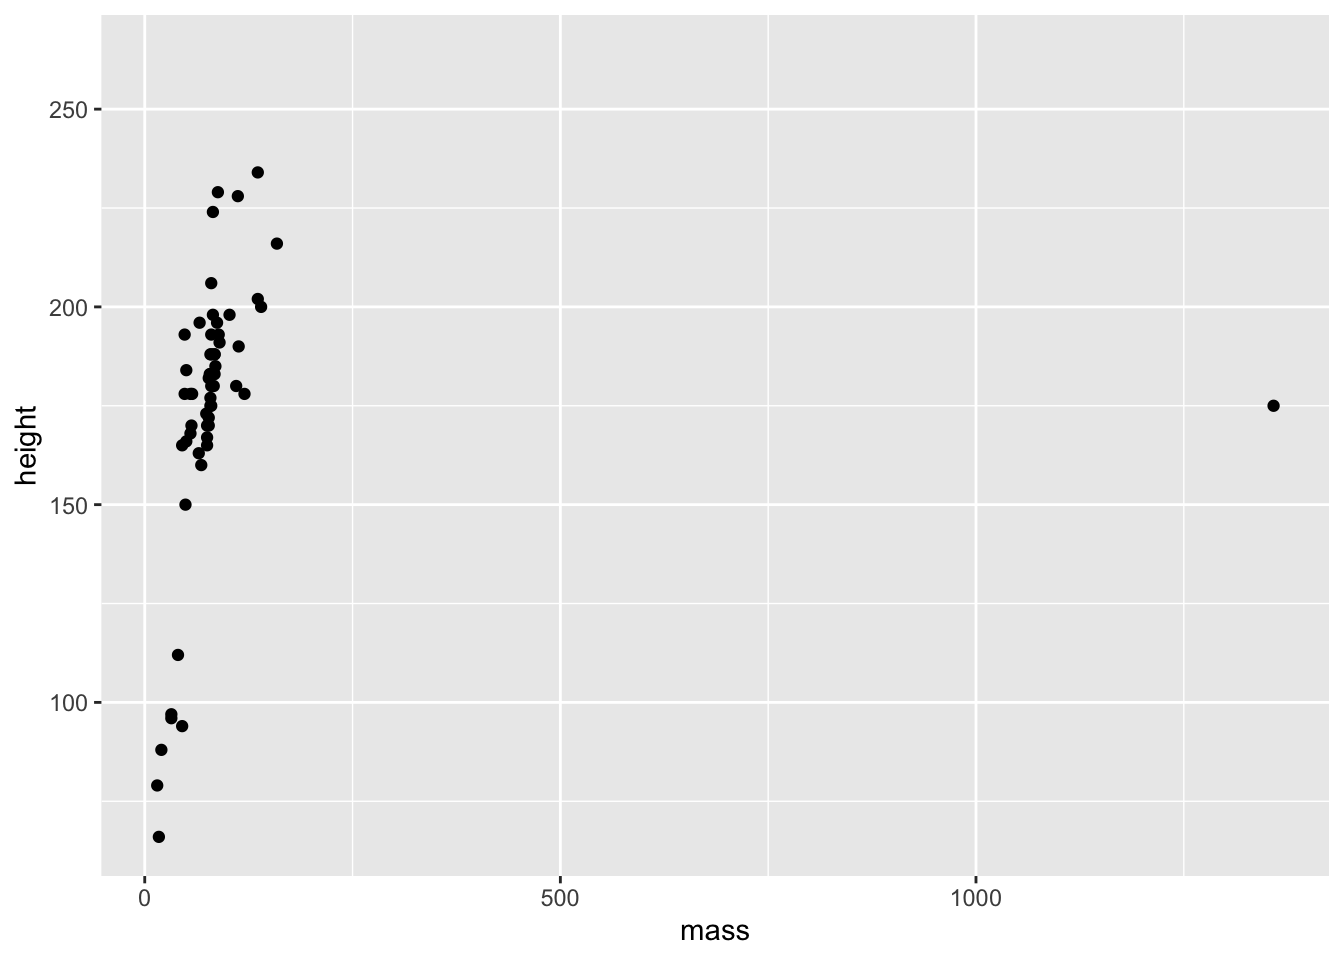
\includegraphics{r4psych_files/figure-latex/2_simple_point_plot-1.pdf}

So, we can see just how easy it is to create a plot of points in ggplot. Well done! There seems to be a positive relationship between mass and height in the starwars data set. We also got a couple of surprises:

\begin{enumerate}
\def\labelenumi{\arabic{enumi}.}
\tightlist
\item
  A warning about 28 rows that contain missing values;
\item
  A really big outlier.
\end{enumerate}

First, we'll explore how ggplot works, then we'll look into these surprises.

The \texttt{ggplot()} function always needs to take a data set. This data set should hold everything you want to plot. Crucially, ggplot builds up the plots in layers. So making the first call \texttt{ggplot(data\ =\ starwars)} tells ggplot where it should look for data, but it doesn't do much else aside from making a grey background.

After this, you need to add some layers to your plot in the form of geometric objects (or geoms, for short). We decided that because we want to look at the link between mass and height, two continuous variables, that adding some points to the plot will be most useful for getting an idea of how the data are related. To do this, we used the \texttt{geom\_point()} function. There are other geoms we could add, but for now we'll focus on points.

Crucially, geom functions take as an argument the mapping in your data. That is, how the visuals of the plot are mapped to your data. This mapping is always defined in terms of the aesthetics of your plot \texttt{aes()}, e.g.~which variables to map onto the x and y axis, in this case.

You can see how this makes ggplot so flexible:

\begin{enumerate}
\def\labelenumi{\arabic{enumi}.}
\tightlist
\item
  Your data argument is flexible, so you can pass different data sets to the same chunk of code by changing out what you pass to the \texttt{data\ =} argument.
\item
  Your aesthetics are flexible, so you can pass different columns to your x and y axis
\item
  Your aesthetics are even more flexible because they can take aesthetics other than just what to plot on the x and y axes
\end{enumerate}

Let's see the flexibility of your aesthetics in action.

\hypertarget{cleaning-before-plotting}{%
\subsection{Cleaning Before Plotting}\label{cleaning-before-plotting}}

We saw before that R gave us a warning that we have rows containing missing values. In this instance, this just means that 28 people weren't plotted because they didn't have height and/or mass values. I'll save filtering data properly (and what the \texttt{\%\textgreater{}\%} (read pipe) symbol does) for another lesson, but we'll get rid of them for now by running this code, below:

\begin{Shaded}
\begin{Highlighting}[]
\NormalTok{filtered\_starwars }\OtherTok{\textless{}{-}}\NormalTok{ starwars }\SpecialCharTok{\%\textgreater{}\%} 
  \FunctionTok{drop\_na}\NormalTok{(height, mass)}
\end{Highlighting}
\end{Shaded}

\hypertarget{changing-your-aesthetics}{%
\subsection{Changing Your Aesthetics}\label{changing-your-aesthetics}}

Let's say we're interested in showing the relationship between mass and height within genders. How can we do this? One way would be to add colour to our the points on the plot in order to highlight the different genders.

\begin{Shaded}
\begin{Highlighting}[]
\FunctionTok{ggplot}\NormalTok{(}\AttributeTok{data =}\NormalTok{ filtered\_starwars) }\SpecialCharTok{+}
  \FunctionTok{geom\_point}\NormalTok{(}\AttributeTok{mapping =} \FunctionTok{aes}\NormalTok{(}\AttributeTok{x =}\NormalTok{ mass, }
                           \AttributeTok{y =}\NormalTok{ height, }
                           \AttributeTok{colour =}\NormalTok{ gender}
\NormalTok{                           )}
\NormalTok{             )}
\end{Highlighting}
\end{Shaded}

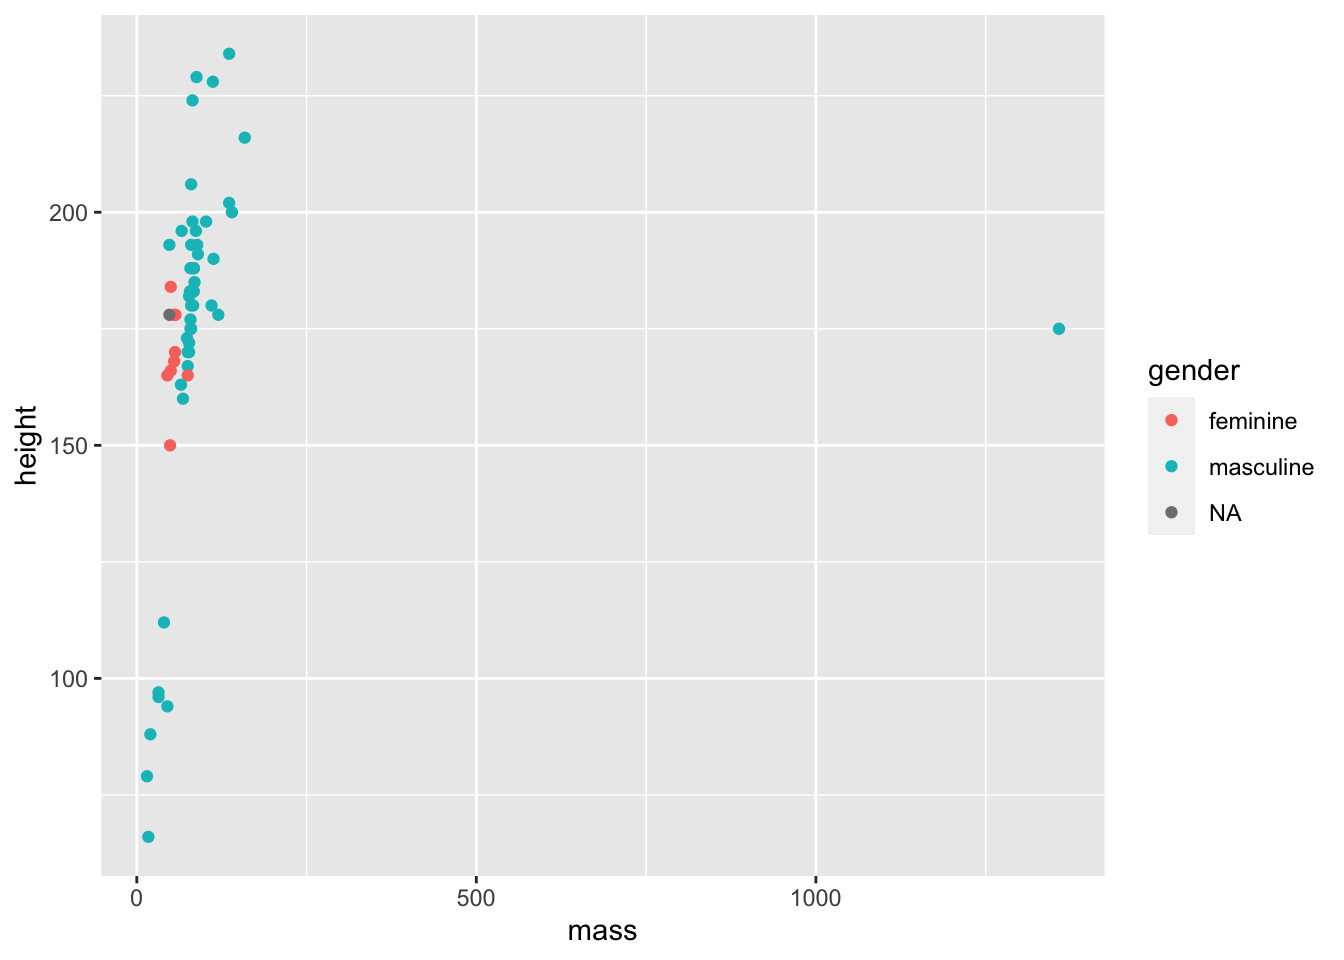
\includegraphics{r4psych_files/figure-latex/2_simple_point_plot_with_colour-1.pdf}

We don't get that warning now that we removed the NAs and passed the filtered data as an argument. That wasn't really necessary as ggplot can handle that for us, but it stops the horrible warning from popping up!

Warnings in R are there to tell you that the output of your code may not contain what you wanted it to contain. In the previous plot, ggplot dropped those with missing heights and masses, even though we didn't explictly tell it to do so. Here, because we filtered those entried with missing values before plotting, we don't get a warning.

Warnings are different to errors in that your code will still work, but you need to check out whether it did what you wanted it to do. On the other hand, errors indicate you did something wrong and your code will fail to run.

Now, we now have colour to see the relationship between mass and height across the genders in the data set. But it's a little difficult to see this relationship given the outlier. Let's see what that outlier is, and whether we should remove it from our data.

Again, you'll learn how this filtering works in later lessons. But for now, I just want to show you how it's useful to understand your data prior to creating a final plot of your data.

\begin{Shaded}
\begin{Highlighting}[]
\NormalTok{filtered\_starwars }\SpecialCharTok{\%\textgreater{}\%} \FunctionTok{filter}\NormalTok{(mass }\SpecialCharTok{\textgreater{}} \DecValTok{1000}\NormalTok{)}
\end{Highlighting}
\end{Shaded}

\begin{verbatim}
## # A tibble: 1 x 14
##   name         height  mass hair_~1 skin_~2 eye_c~3 birth~4 sex   gender homew~5
##   <chr>         <int> <dbl> <chr>   <chr>   <chr>     <dbl> <chr> <chr>  <chr>  
## 1 Jabba Desil~    175  1358 <NA>    green-~ orange      600 herm~ mascu~ Nal Hu~
## # ... with 4 more variables: species <chr>, films <list>, vehicles <list>,
## #   starships <list>, and abbreviated variable names 1: hair_color,
## #   2: skin_color, 3: eye_color, 4: birth_year, 5: homeworld
\end{verbatim}

\begin{Shaded}
\begin{Highlighting}[]
\CommentTok{\# overwrite data to remove outlier (keep all with mass below 1000)}
\CommentTok{\# filtered\_starwars \textless{}{-} filtered\_starwars \%\textgreater{}\% filter(mass \textless{} 1000) \# not run}
\end{Highlighting}
\end{Shaded}

Of course, it's Jabba the Hutt. We could choose to throw Jabba out of our data by using the code above to overwrite the data (commented out), but for now, we'll see just how powerful ggplot is without throwing away our data.

\begin{Shaded}
\begin{Highlighting}[]
\FunctionTok{ggplot}\NormalTok{(}\AttributeTok{data =}\NormalTok{ filtered\_starwars) }\SpecialCharTok{+}
  \FunctionTok{geom\_point}\NormalTok{(}\AttributeTok{mapping =} \FunctionTok{aes}\NormalTok{(}\AttributeTok{x =}\NormalTok{ mass, }
                           \AttributeTok{y =}\NormalTok{ height, }
                           \AttributeTok{colour =}\NormalTok{ gender}
\NormalTok{                           )}
\NormalTok{             ) }\SpecialCharTok{+}
  \FunctionTok{coord\_cartesian}\NormalTok{(}\AttributeTok{xlim =} \FunctionTok{c}\NormalTok{(}\DecValTok{0}\NormalTok{, }\DecValTok{180}\NormalTok{))}
\end{Highlighting}
\end{Shaded}

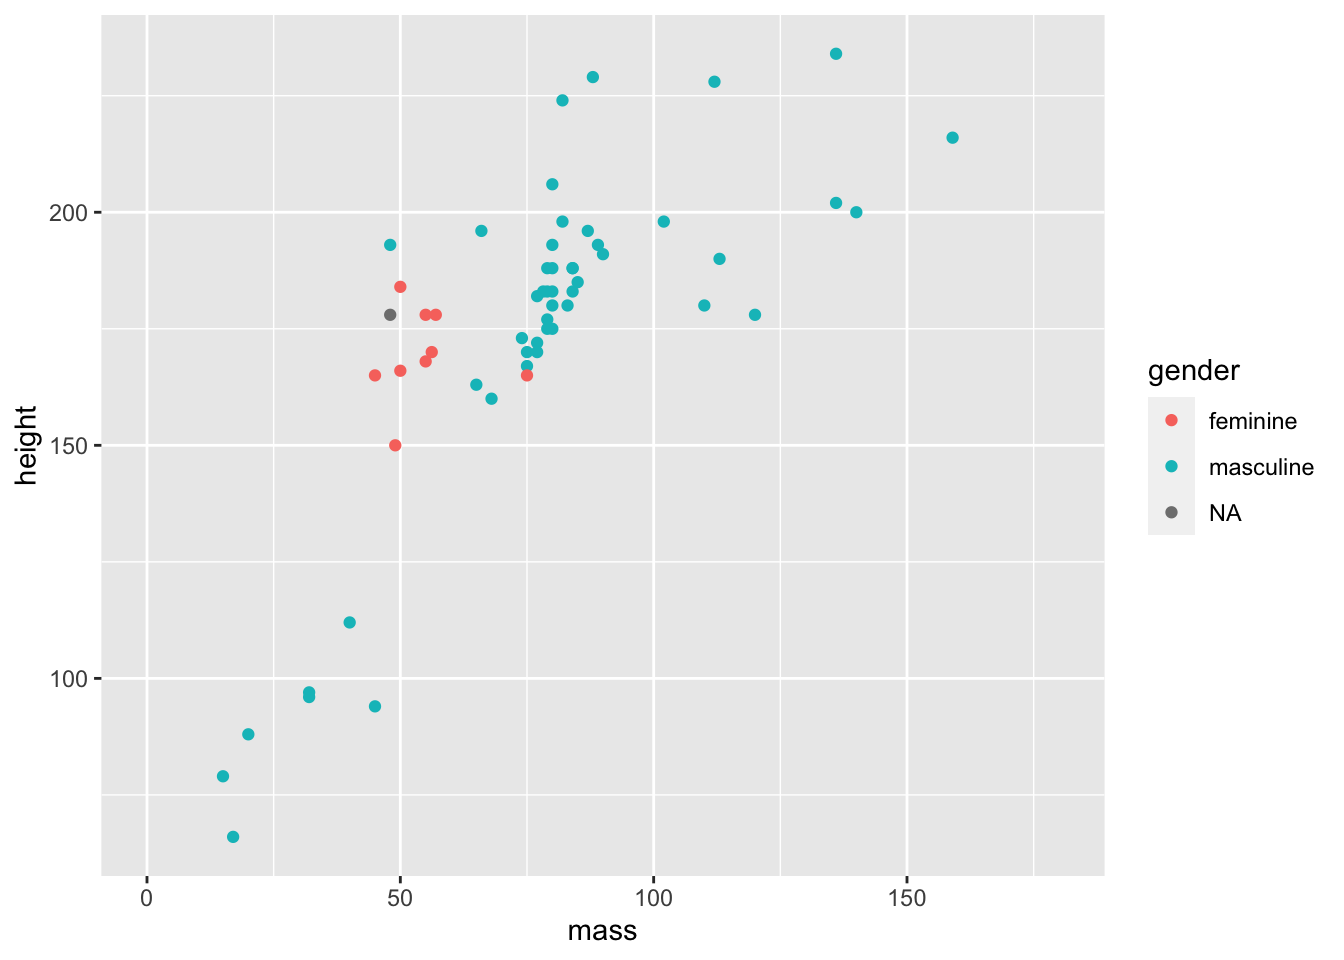
\includegraphics{r4psych_files/figure-latex/2_replot_point_plot_with_colour-1.pdf}

This time we added a function \texttt{coord\_cartesian()} to the end of our \texttt{ggplot()} call. We defined the limits of the x axis to be between 0 and 180. This way, we can get a better look at the trends in our data.

Why do we define limits inside this function? Well, we could have also manually defined the scale with \texttt{scale\_x\_continuous(limits\ =\ c(0,\ 180))}. This may seem more inuitive, but it throws out the data points outside the limits prior to plotting. Why is this a problem? ggplot has some nice functionalities such as drawing lines of best fit for you based on the data in the plot. If you throw data away while plotting, your line of best fit will shift. So, if you decide that you want to change your scale but keep your model fits for all data, use \texttt{coord\_cartesian()}.

Given this is an outlier, your choice doesn't matter if you're just trying to show trends like this, but your choice is important if you want to show any inferential statistics associated with the data.

Next up, we'll look at changing a few components of the points on the plot.

\begin{Shaded}
\begin{Highlighting}[]
\FunctionTok{ggplot}\NormalTok{(}\AttributeTok{data =}\NormalTok{ filtered\_starwars) }\SpecialCharTok{+}
  \FunctionTok{geom\_point}\NormalTok{(}\AttributeTok{mapping =} \FunctionTok{aes}\NormalTok{(}\AttributeTok{x =}\NormalTok{ mass, }
                           \AttributeTok{y =}\NormalTok{ height, }
                           \AttributeTok{colour =}\NormalTok{ gender}
\NormalTok{                           ),}
             \AttributeTok{alpha =} \FloatTok{0.7}\NormalTok{, }\CommentTok{\# opacity}
             \AttributeTok{shape =} \DecValTok{17}\NormalTok{, }\CommentTok{\# triangles}
             \AttributeTok{size =} \DecValTok{4}\NormalTok{) }\SpecialCharTok{+} \CommentTok{\# bigger points}
  \FunctionTok{coord\_cartesian}\NormalTok{(}\AttributeTok{xlim =} \FunctionTok{c}\NormalTok{(}\DecValTok{0}\NormalTok{, }\DecValTok{180}\NormalTok{))}
\end{Highlighting}
\end{Shaded}

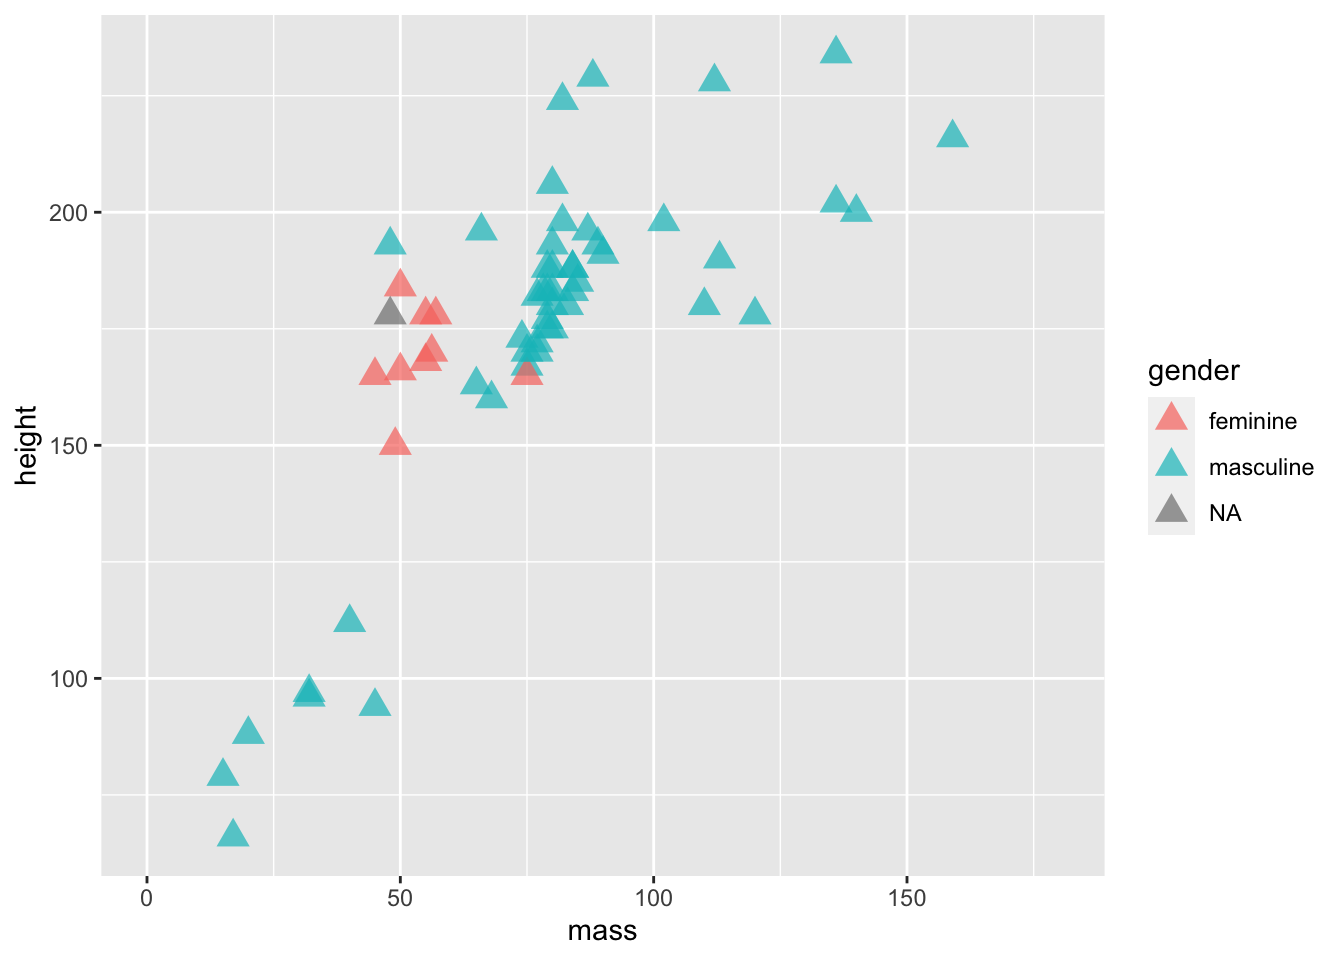
\includegraphics{r4psych_files/figure-latex/2_adding_constant_visual_changes_to_plots-1.pdf}

We've added 3 variables outside of the \texttt{aes()} mapping. This means that all of the points within the plot are changed in the same way:

\begin{enumerate}
\def\labelenumi{\arabic{enumi}.}
\tightlist
\item
  They all become a little bit transparent through the \texttt{alpha} variable definition;
\item
  They all take a triangle shape through the \texttt{shape} variable definition (and the number associated)
\item
  They are all the same size due to the \texttt{size} variable definition.
\end{enumerate}

If we put these variables within the \texttt{aes()} mappings and associated them with a variable within the data set, such as \texttt{gender}, then each point would be affected differently depending on which level of the gender factor the individual data points belong to. It's important to remember that everything within \texttt{aes()} is mapped onto variables with which to display your data. So, the x location, y location, and anything else that you define within \texttt{aes()} can vary by your data set. Everything outside of it will affect all levels of your data.

Here, we'll define colour both within and outside the \texttt{aes()} mapping, causing a clash. Try this plot below to see how clashes are resolved in ggplot:

\begin{Shaded}
\begin{Highlighting}[]
\FunctionTok{ggplot}\NormalTok{(}\AttributeTok{data =}\NormalTok{ filtered\_starwars) }\SpecialCharTok{+}
  \FunctionTok{geom\_point}\NormalTok{(}\AttributeTok{mapping =} \FunctionTok{aes}\NormalTok{(}\AttributeTok{x =}\NormalTok{ mass, }
                           \AttributeTok{y =}\NormalTok{ height, }
                           \AttributeTok{colour =}\NormalTok{ gender}
\NormalTok{                           ),}
             \AttributeTok{colour =} \StringTok{"red"}\NormalTok{) }\SpecialCharTok{+}
  \FunctionTok{coord\_cartesian}\NormalTok{(}\AttributeTok{xlim =} \FunctionTok{c}\NormalTok{(}\DecValTok{0}\NormalTok{, }\DecValTok{180}\NormalTok{))}
\end{Highlighting}
\end{Shaded}

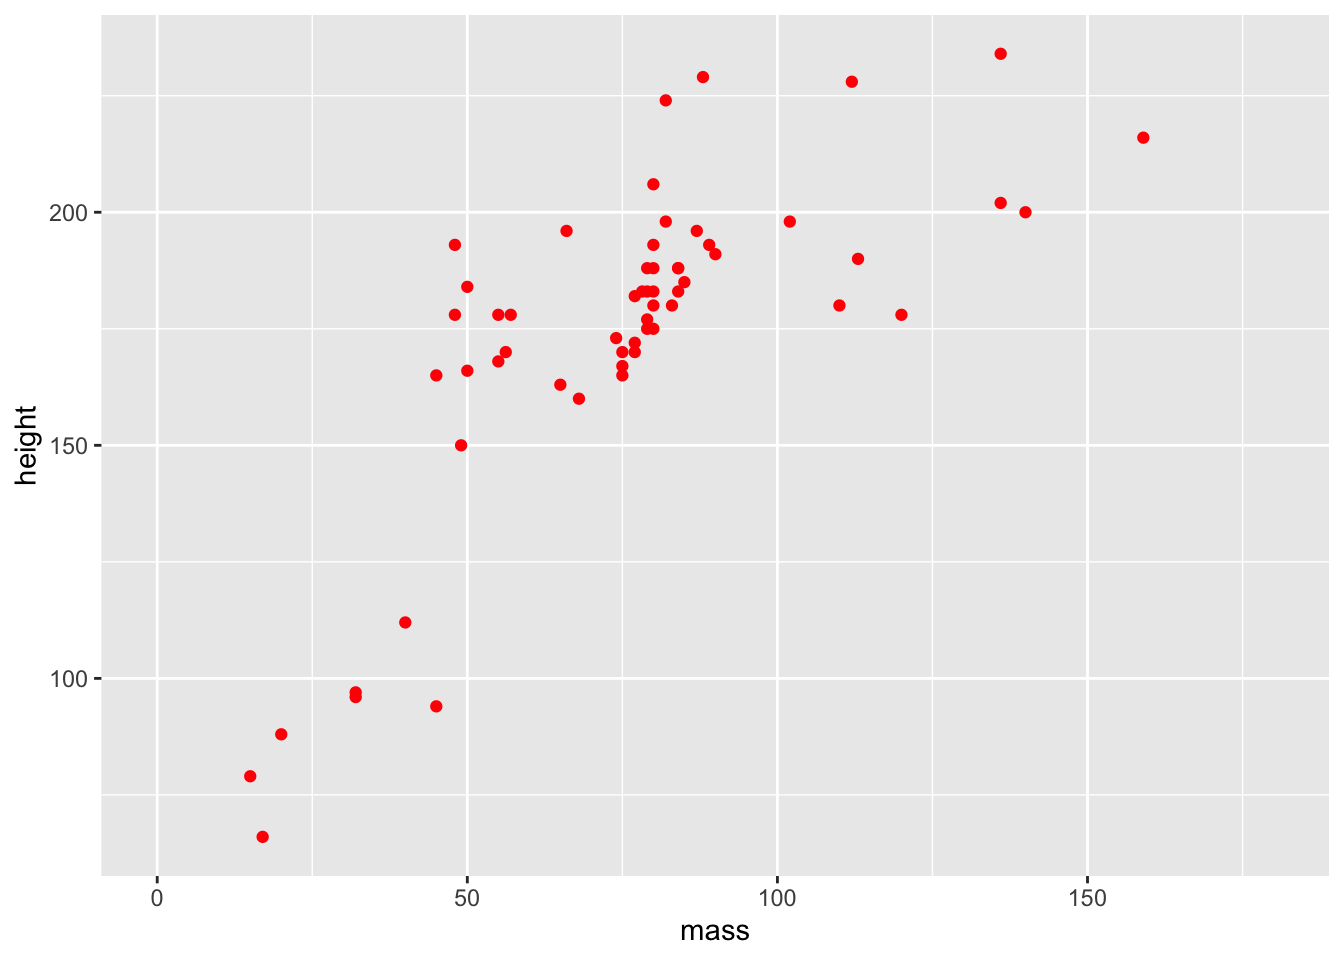
\includegraphics{r4psych_files/figure-latex/2_clashes_with_aes_and_constants_within_plots-1.pdf}

The different colours for each level of gender are now gone, along with the legend! Our variable definition for \texttt{colour} outside of the \texttt{aes()} mappings overrides that within \texttt{aes()}. This is because we've manually set the aesthetic properties of our plot by defining colour as an argument of the geom function, rather than of the aethetic mapping.

R has some built in shapes that we can define within our plots. For shapes, these are divided into three categories:

\begin{itemize}
\tightlist
\item
  Colour border with hollow fill (0 - 14)
\item
  Colourless border with colour fill (15 - 18)
\item
  Colour border with colour fill (21 - 24)
\end{itemize}

Bear in mind that colour and fill are different properties that we can control within our plots. Below, I've used hex values to specify the exact colours that I'd like for the colour (around the border) and the fill for our points. You can find a nice hex selector at \href{http://htmlcolorcodes.com/}{htmlcolorcodes.com} which will allow you to customise your plot colours to your liking. Just change the letters and numbers after the \texttt{\#} in the \texttt{colour} call, and you can change the colours to your liking.

In the example below I chose my colours based on the diverging colourblind safe selection of colours from \href{http://colorbrewer2.org/\#type=sequential\&scheme=BuGn\&n=3}{Color Brewer}. I'd recommend that you use this if you're going to include colour in any plots for papers/presentations.

\begin{Shaded}
\begin{Highlighting}[]
\FunctionTok{ggplot}\NormalTok{(}\AttributeTok{data =}\NormalTok{ filtered\_starwars, }\AttributeTok{na.rm =}\NormalTok{ T) }\SpecialCharTok{+}
  \FunctionTok{geom\_point}\NormalTok{(}\AttributeTok{mapping =} \FunctionTok{aes}\NormalTok{(}\AttributeTok{x =}\NormalTok{ mass, }
                           \AttributeTok{y =}\NormalTok{ height, }
                           \AttributeTok{colour =}\NormalTok{ gender}
\NormalTok{                           ),}
             \AttributeTok{colour =} \StringTok{"\#af8dc3"}\NormalTok{,}
             \AttributeTok{fill =} \StringTok{"\#7fbf7b"}\NormalTok{,}
             \AttributeTok{shape =} \DecValTok{21}\NormalTok{,}
             \AttributeTok{size =} \DecValTok{8}\NormalTok{,}
             \AttributeTok{stroke =} \DecValTok{3}
\NormalTok{             ) }\SpecialCharTok{+}
  \FunctionTok{coord\_cartesian}\NormalTok{(}\AttributeTok{xlim =} \FunctionTok{c}\NormalTok{(}\DecValTok{0}\NormalTok{, }\DecValTok{180}\NormalTok{))}
\end{Highlighting}
\end{Shaded}

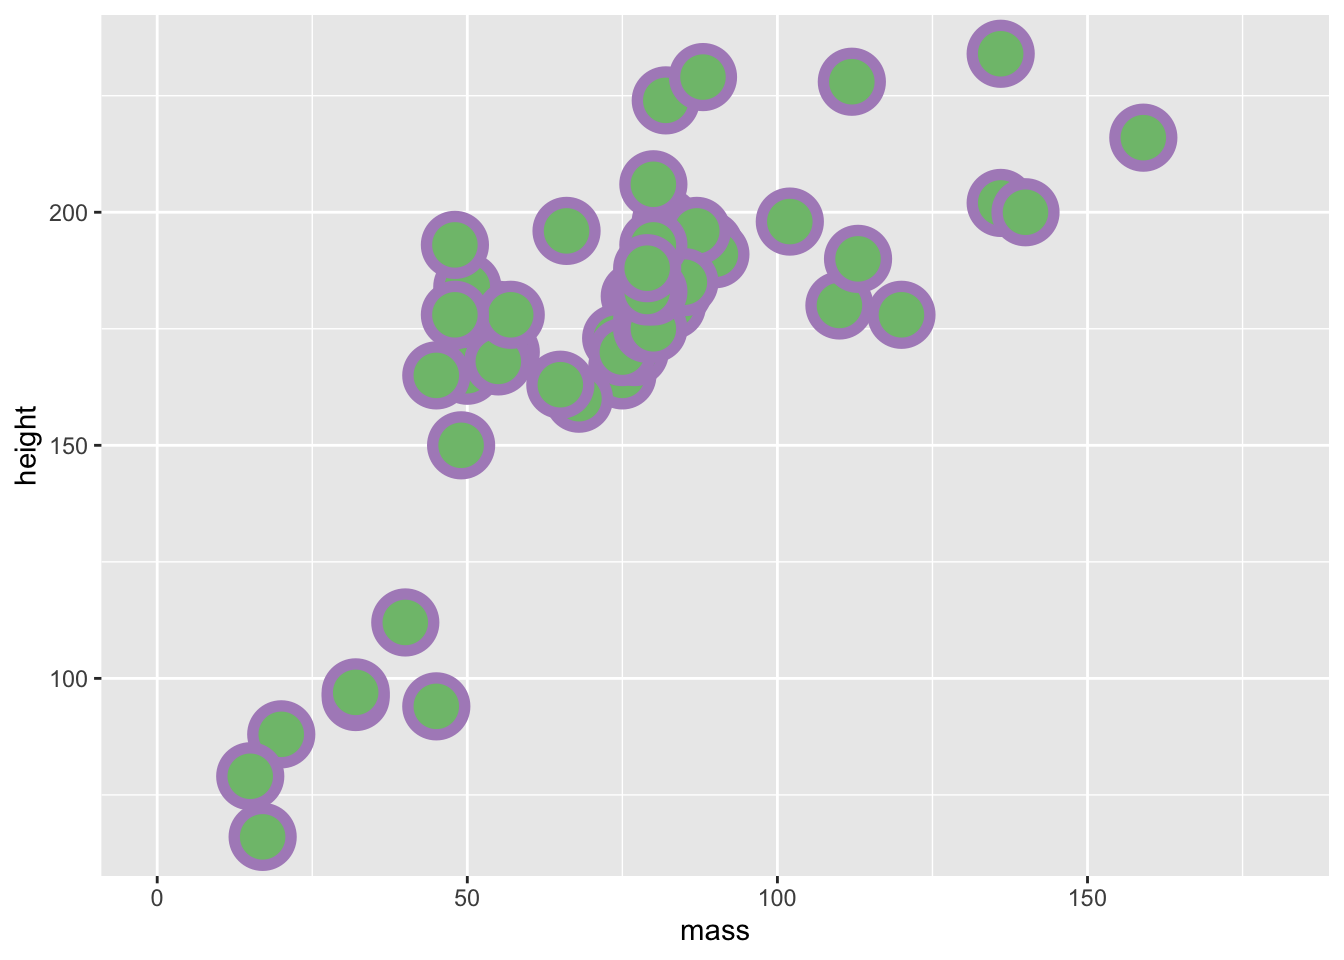
\includegraphics{r4psych_files/figure-latex/2_colour_and_fill-1.pdf}

Try to mess about with the different definitions that we provided above. Change the colour, size, and stroke values to see how these variables work.

We've used the aesthetics above to define categorical data by colour. But what happens if we use continuous data?

\begin{Shaded}
\begin{Highlighting}[]
\FunctionTok{ggplot}\NormalTok{(}\AttributeTok{data =}\NormalTok{ filtered\_starwars, }\AttributeTok{na.rm =}\NormalTok{ T) }\SpecialCharTok{+}
  \FunctionTok{geom\_point}\NormalTok{(}\AttributeTok{mapping =} \FunctionTok{aes}\NormalTok{(}\AttributeTok{x =}\NormalTok{ mass, }
                           \AttributeTok{y =}\NormalTok{ height, }
                           \AttributeTok{colour =}\NormalTok{ birth\_year}
\NormalTok{                           )}
\NormalTok{             ) }\SpecialCharTok{+}
  \FunctionTok{coord\_cartesian}\NormalTok{(}\AttributeTok{xlim =} \FunctionTok{c}\NormalTok{(}\DecValTok{0}\NormalTok{, }\DecValTok{180}\NormalTok{))}
\end{Highlighting}
\end{Shaded}

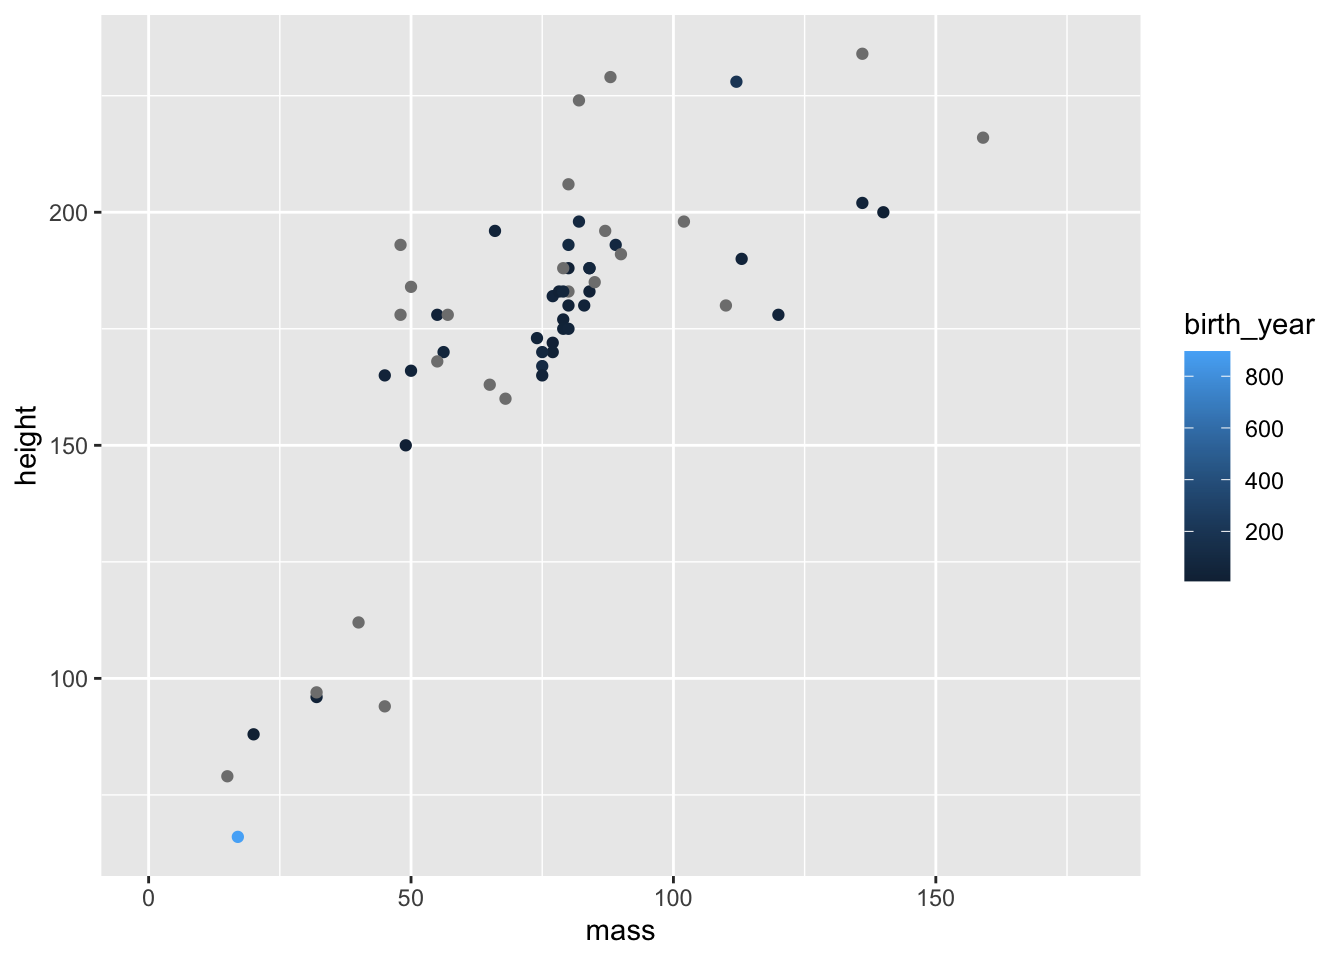
\includegraphics{r4psych_files/figure-latex/2_colour_gradient-1.pdf}

You can see that we get a sliding scale for the hue of the points. Pretty neat, but also quite difficult to get a real idea of where on the scale the points lie.

There are many inbuilt plots that you can create with ggplot2 by mapping your data to different geoms. To get an idea of all of different types of geoms, type \texttt{??geom}. This should give you an index of all of the geom types available to ggplot2 in your Help pane of RStudio.

\hypertarget{exploring-different-geoms}{%
\section{Exploring Different Geoms}\label{exploring-different-geoms}}

You've already learned about \texttt{geom\_point()} above, but now we'll explore the other geom types.

For this exploration, we'll use a different data set with a limited number of groups for ease of visualisation. I've simulated some data for this exercise. You can find this data in the inputs folder for this lesson. (If you're interested, you can also find the script for generating this data in the data\_generation folder).

Let's load this data into R. Here, we use the function \texttt{read\_csv} rather than the base R \texttt{read.csv}. This is because \texttt{read\_csv} is faster, typically does a better job at guessing the data types for your columns of data, and saves the output as a tibble.

\emph{Note}: \texttt{read\_csv} will try to guess the types of data in each column for a data set loaded into R, but sometimes it can fail. We'll cover instances where this fails, and how to remedy it, in the next lesson.

\begin{Shaded}
\begin{Highlighting}[]
\NormalTok{rt\_data }\OtherTok{\textless{}{-}} \FunctionTok{read\_csv}\NormalTok{(}\StringTok{"inputs/rt\_data.csv"}\NormalTok{)}
\end{Highlighting}
\end{Shaded}

How should we interpret this data? Imagine that we ran a lexical decision task on two groups of participants. In one condition, participants responded to sentences such as \emph{``Eric turned down the volume''}, and had to indicate whether this sentence made sense by turning a knob. In the match condition, agreement matched the motion indicated in the sentence (e.g.~left = yes, it makes sense), and in the mismatch condition agreement did not match the motion indicated in the sentence (e.g.~right = yes, it makes sense). \href{http://psycnet.apa.org/record/2006-01956-001}{Zwaan and Taylor (2006, Experiment 4)} hypothesised that when the action and response are matched, resposne times should be quicker than if they do not match.

The \texttt{participant} column indicates individual participants, the \texttt{gender} column indicates the gender of our participants, \texttt{response\_condition} indicates whether participants took part in the match or mismatch conditions, and \texttt{reaction\_time}, our dependent variable, represents the average reaction time in milliseconds for each participant to respond to whether or not the sentences made sense.

\hypertarget{bar-plots}{%
\subsection{Bar Plots}\label{bar-plots}}

Bar plots are one of the most common plots you'll come across in Psychology. They're most useful for representing counts of data that are divided into categories. For example, you could use a bar plot to show the number of male and female participants in your study. Using our simulated data set, we can use a bar plot to show the counts of males and females in our data set.

\begin{Shaded}
\begin{Highlighting}[]
\FunctionTok{ggplot}\NormalTok{(}\AttributeTok{data =}\NormalTok{ rt\_data, }
       \AttributeTok{mapping =} \FunctionTok{aes}\NormalTok{(}\AttributeTok{x =}\NormalTok{ gender)}
\NormalTok{       ) }\SpecialCharTok{+}
  \FunctionTok{geom\_bar}\NormalTok{()}
\end{Highlighting}
\end{Shaded}

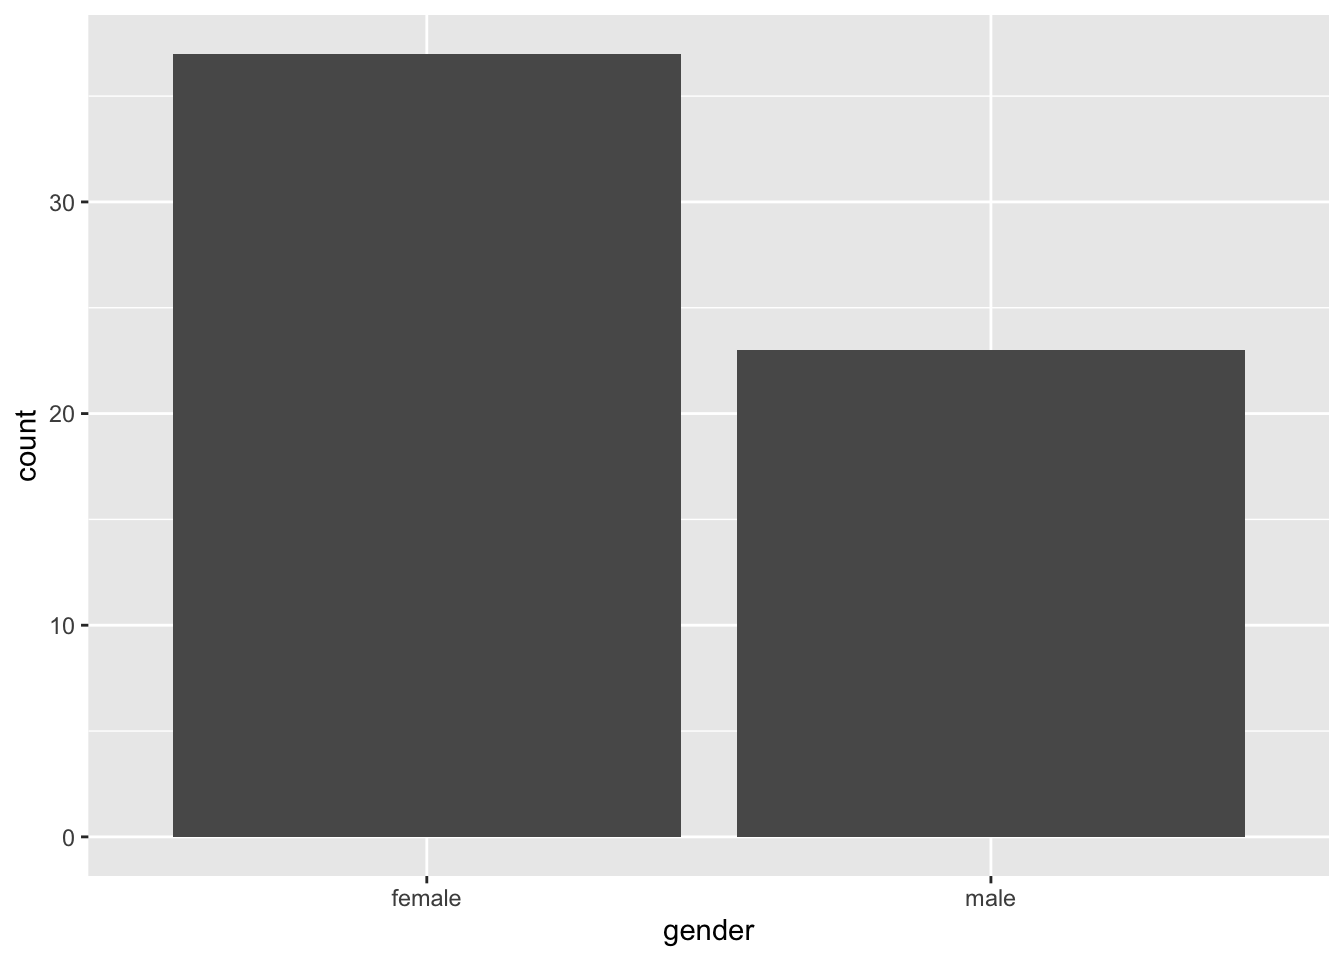
\includegraphics{r4psych_files/figure-latex/2_bar_plot-1.pdf}

You'll often find that psychologists like to plot continuous data in a bar plot. I've done this myself, but we can do better. One alternative would be to use a boxplot, a violin plot, or even a pirate plot which we'll explore in the next lesson (well, we are plotting with Rrrrrrrrr\ldots).

Since we've got data which represents mean scores for each participant, this will be suitable for plotting straight away. If, however, you have raw data, remember to aggregate by participants or items prior to plotting. We'll cover this in later classes.

\hypertarget{box-plots}{%
\subsection{Box Plots}\label{box-plots}}

Box plots provide a better way to represent continuous outcomes (such as reaction times) than bar plots as they give you more information about the variance within your data set.

\hypertarget{how-to-read-a-box-plot}{%
\subsubsection{How to read a box plot}\label{how-to-read-a-box-plot}}

\begin{itemize}
\tightlist
\item
  The middle line represents the median
\item
  The upper white section of the box the upper quartile: 75\% of scores fall below this.
\item
  The lower white section the lower quartile: 25\% of scores fall below this.
\item
  Together the quartiles represent the interquartile range: The middle 50\% of scores.
\item
  The limits of the whiskers (black lines) for the upper and lower parts of the graph represent the smallest and largest observations that are equal to the upper or lower quartiles minus or plus 1.5 times the interquartile range. Effectively, this is most of the rest of the data, apart from outliers.
\item
  The dots represent outliers (i.e.~those values outside of the whiskers)
\end{itemize}

\begin{Shaded}
\begin{Highlighting}[]
\FunctionTok{ggplot}\NormalTok{(}\AttributeTok{data =}\NormalTok{ rt\_data, }
       \AttributeTok{mapping =} \FunctionTok{aes}\NormalTok{(}\AttributeTok{x =}\NormalTok{ response\_condition, }
                     \AttributeTok{y =}\NormalTok{ reaction\_time}
\NormalTok{                     )}
\NormalTok{       ) }\SpecialCharTok{+}
  \FunctionTok{geom\_boxplot}\NormalTok{()}
\end{Highlighting}
\end{Shaded}

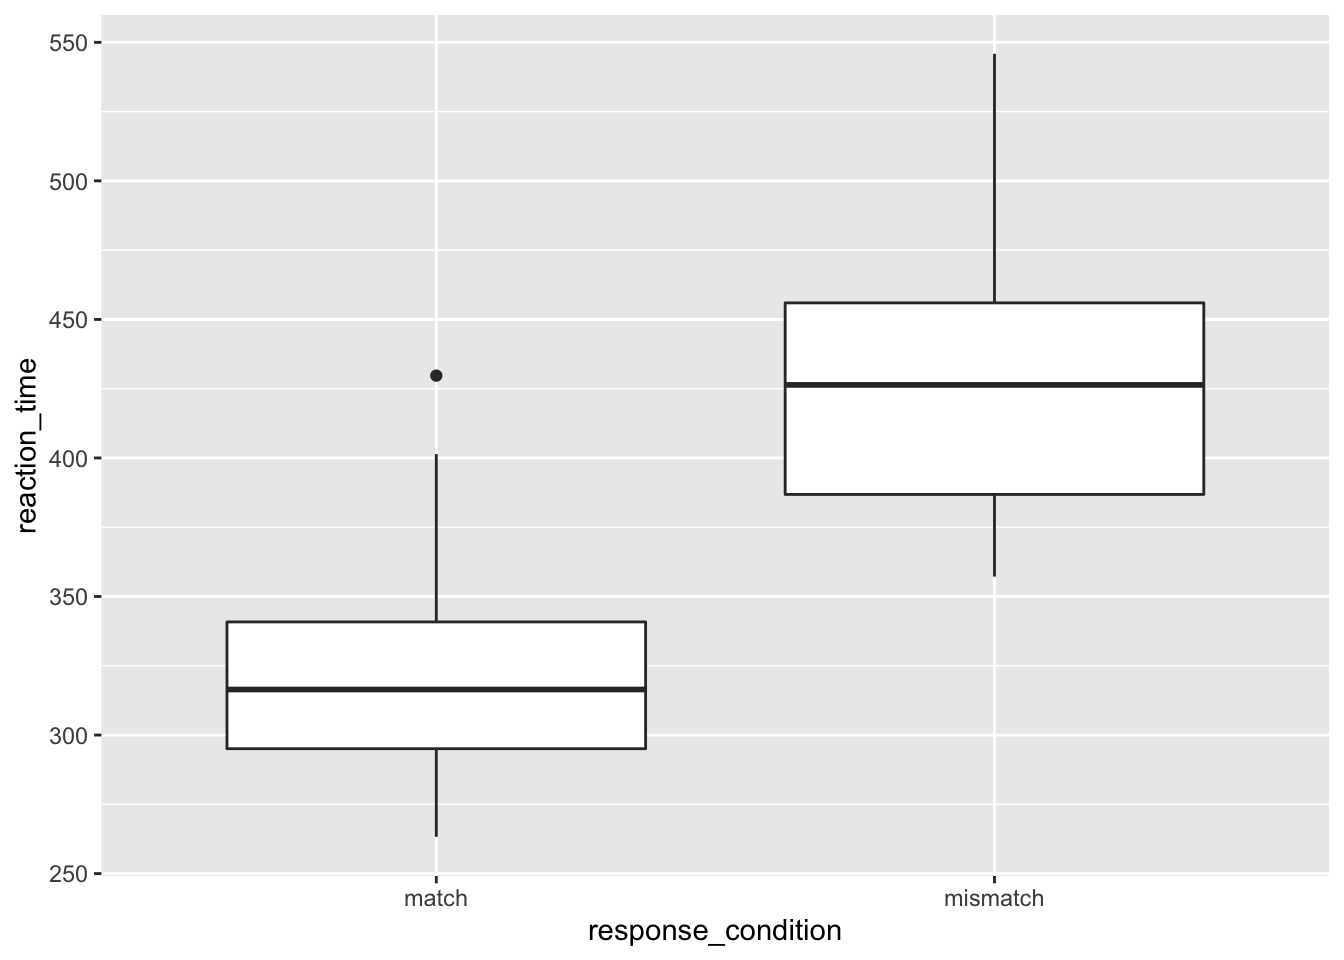
\includegraphics{r4psych_files/figure-latex/2_box_plot-1.pdf}

We can see that the median reaction time is highest for those in the mismatch condition. Notice also that the interquartile range is larger, and so is the upper limit of the whiskers. This all suggests that those in the mismatch group vary more from each other than those in the match condition.

Also, notice the outlier in the match group. Someone obviously has a very slow reaction time compared to the rest of the cohort. I wonder why that could be? Perhaps it's because they misinterpreted the instructions, accidentally putting themselves into the mismatch condition. Or, it could be because I simulated this data and didn't control for how outliers were distributed.

\hypertarget{violin-plots}{%
\subsection{Violin Plots}\label{violin-plots}}

Additionally, we have violin plots which show you the density of the mean scores. The wider the section of the violin, the more scores around that area. We set \texttt{trim} to \texttt{FALSE} within the violin plot so that we see the full tails of the data. If we set this to \texttt{TRUE}, then the tails are trimmed to the range of the data.

It's also useful to draw quantiles on the violin plot, so we can see the quantiles as with the box plot using \texttt{draw\_quantiles} and by specifying where we want these quantiles. Here, we chose the upper and lower 25\% and the interquartile range.

\begin{Shaded}
\begin{Highlighting}[]
\FunctionTok{ggplot}\NormalTok{(}\AttributeTok{data =}\NormalTok{ rt\_data, }
       \AttributeTok{mapping =} \FunctionTok{aes}\NormalTok{(}\AttributeTok{x =}\NormalTok{ response\_condition, }
                     \AttributeTok{y =}\NormalTok{ reaction\_time}
\NormalTok{                     )}
\NormalTok{       ) }\SpecialCharTok{+}
  \FunctionTok{geom\_violin}\NormalTok{(}
    \AttributeTok{trim =} \ConstantTok{FALSE}\NormalTok{,}
    \AttributeTok{draw\_quantiles =} \FunctionTok{c}\NormalTok{(}\FloatTok{0.25}\NormalTok{, }\FloatTok{0.5}\NormalTok{, }\FloatTok{0.75}\NormalTok{)}
\NormalTok{    )}
\end{Highlighting}
\end{Shaded}

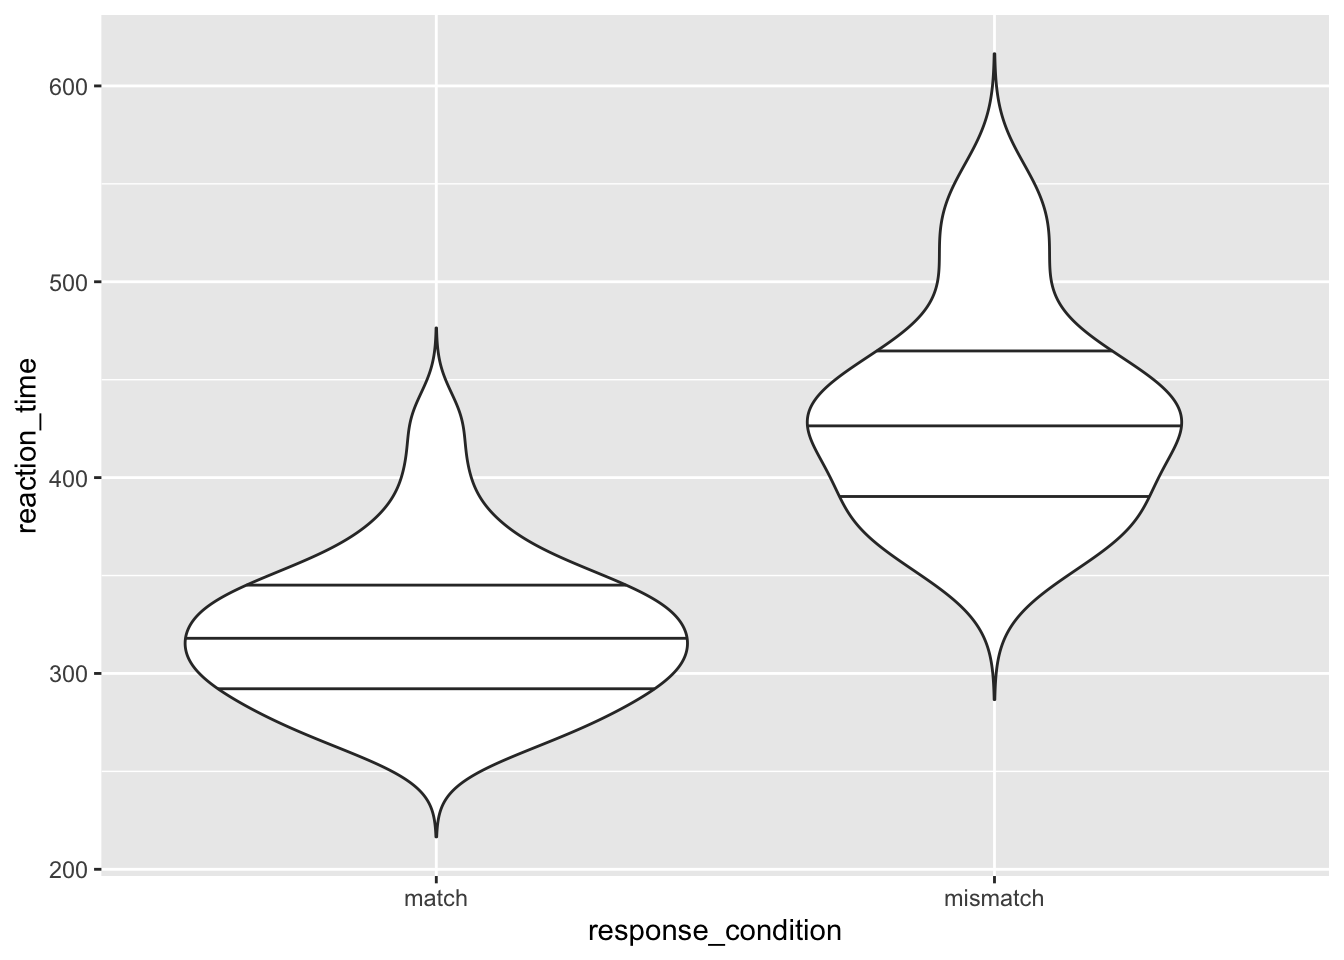
\includegraphics{r4psych_files/figure-latex/2_violin_plot-1.pdf}

\hypertarget{density-plots}{%
\subsection{Density Plots}\label{density-plots}}

Now we'll look at ways to check for the distribution of your continuous variables. This is a good way to get an eye for whether or not your data are skewed and require a transformation on the data, or a non-parametric test when it comes to inferential statistics. Again, we'll return to what this means in regards to statistics later in this course, but for now it's a good idea to understand how you can check the distribution of your data prior to computing any statistics.

We've added the additional argument \texttt{fill} to the aethetic mapping, to specify that we wanted different colours for our groups. We also specified the additional argument \texttt{alpha} in our density plot to specify that we wanted some opacity to the densities.

\begin{Shaded}
\begin{Highlighting}[]
\FunctionTok{ggplot}\NormalTok{(}\AttributeTok{data =}\NormalTok{ rt\_data, }
       \AttributeTok{mapping =} \FunctionTok{aes}\NormalTok{(}\AttributeTok{x =}\NormalTok{ reaction\_time, }
                     \AttributeTok{fill =}\NormalTok{ response\_condition}
\NormalTok{                     )}
\NormalTok{       ) }\SpecialCharTok{+}
  \FunctionTok{geom\_density}\NormalTok{(}\AttributeTok{alpha =} \FloatTok{0.5}\NormalTok{) }\CommentTok{\# alpha = opacity}
\end{Highlighting}
\end{Shaded}

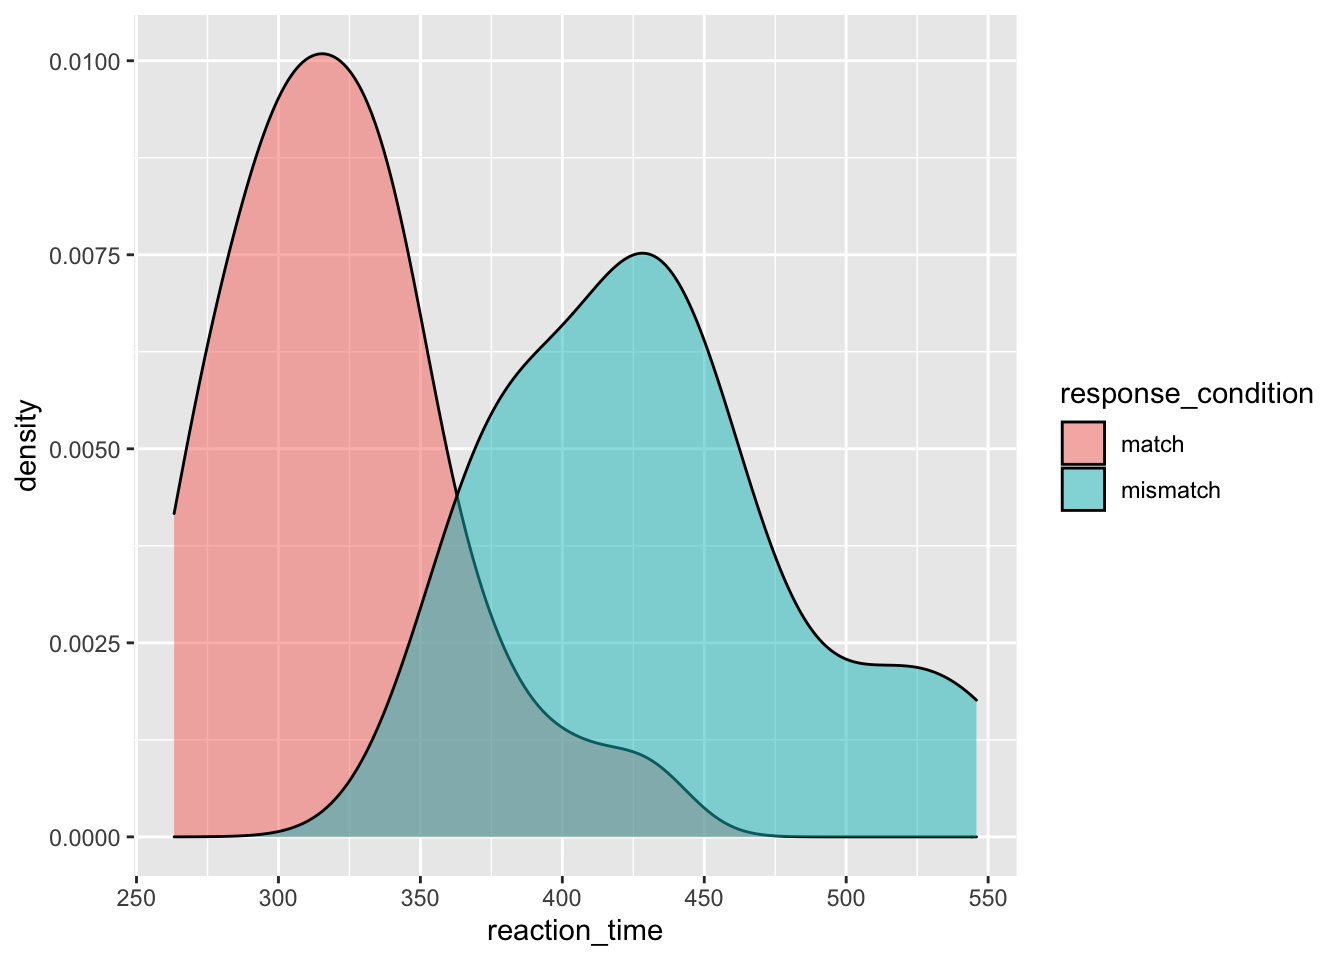
\includegraphics{r4psych_files/figure-latex/2_density_plot-1.pdf}

\hypertarget{histograms}{%
\subsection{Histograms}\label{histograms}}

If you have relatively few observations, a histogram may be more appropriate than a density plot. But, we'll just stick to the same data as before to see how this works.
Here, it's often useful to set the \texttt{binwidth} prior to plotting. ggplot will try to set it to a default if it can, but this may not be what you want. Here, we've set the \texttt{binwidth} to 50, so we count how many observations we have for reaction times in 50ms bins, i.e.~from 225 to 275ms, from 275 to 325ms etc. We also set the \texttt{fill} of the bars to white, and the \texttt{colour} to black so we get white bars with a black outline.

\begin{Shaded}
\begin{Highlighting}[]
\FunctionTok{ggplot}\NormalTok{(}\AttributeTok{data =}\NormalTok{ rt\_data, }\AttributeTok{mapping =} \FunctionTok{aes}\NormalTok{(}\AttributeTok{x =}\NormalTok{ reaction\_time)) }\SpecialCharTok{+}
  \FunctionTok{geom\_histogram}\NormalTok{(}\AttributeTok{binwidth =} \DecValTok{50}\NormalTok{, }
                 \AttributeTok{fill =} \StringTok{"white"}\NormalTok{, }
                 \AttributeTok{colour =} \StringTok{"black"}
\NormalTok{                 )}
\end{Highlighting}
\end{Shaded}

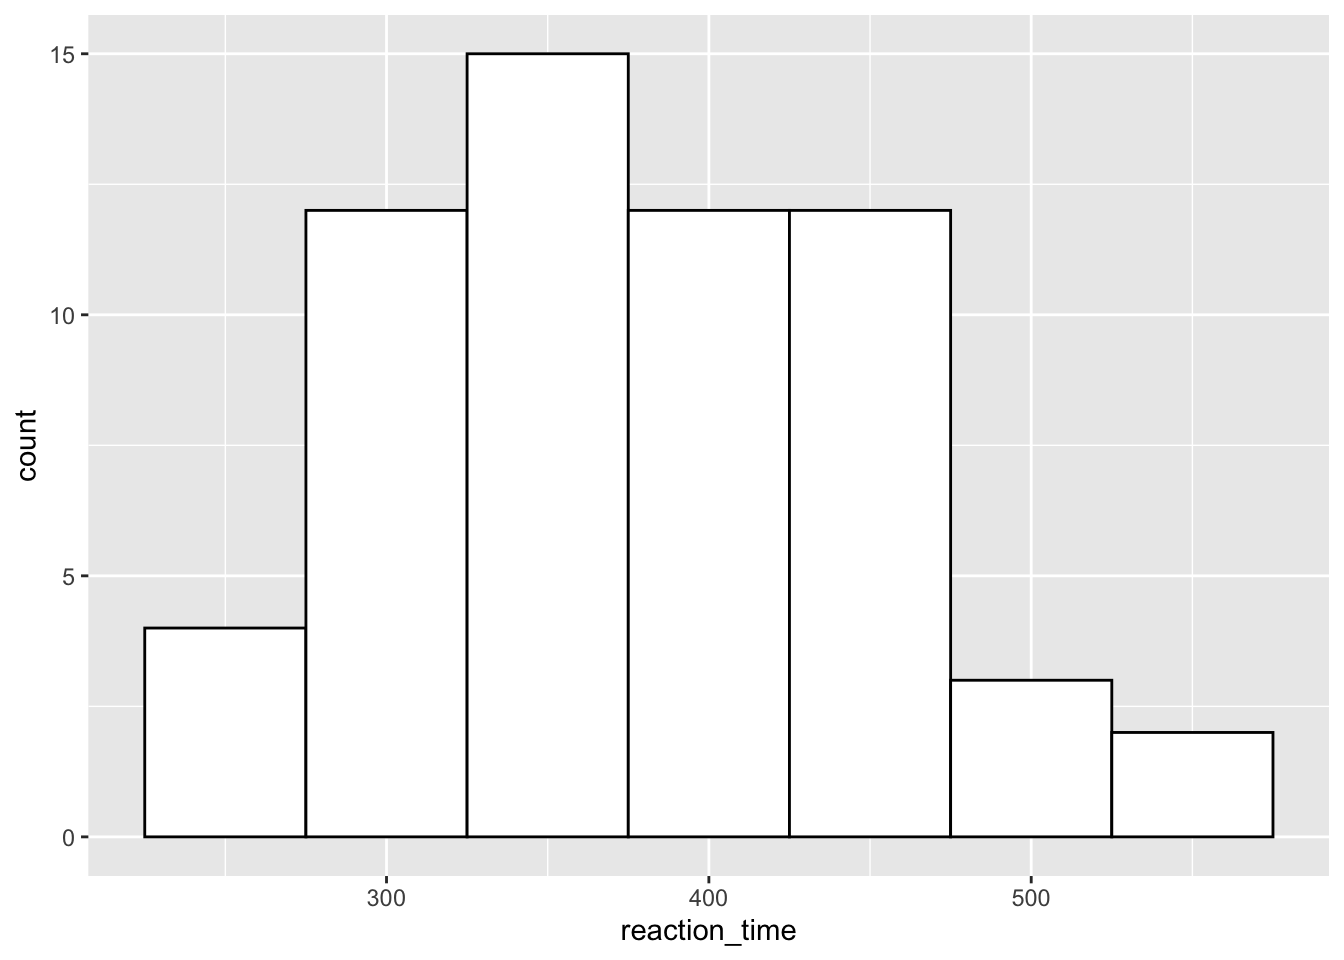
\includegraphics{r4psych_files/figure-latex/2_histogram_plot-1.pdf}

\hypertarget{exercises-1}{%
\section{Exercises}\label{exercises-1}}

If that's not enough to make you fall \href{https://youtu.be/hO-UyFL5cxY}{asleep}, try out the exercises below. We'll cover these in the class with the solutions uploaded at the beginning of each session in a separate downloadable link. Try to solve these questions before resorting to the solutions. I'll be there to help out where necessary.

In this section, we'll use some new data from the pre-packaged data sets in R. First off, we'll load the \texttt{chickwts} data set, which looks at chicken weights by different feed types.

\begin{Shaded}
\begin{Highlighting}[]
\FunctionTok{data}\NormalTok{(chickwts)}
\end{Highlighting}
\end{Shaded}

\hypertarget{main-exercises}{%
\subsection{Main Exercises}\label{main-exercises}}

\hypertarget{question-1-1}{%
\subsection{Question 1}\label{question-1-1}}

Take a look at the first 6 rows of the data set. How does the data look? Is this appropriate for plotting?

\hypertarget{question-2-1}{%
\subsection{Question 2}\label{question-2-1}}

Calculate the overall means for the chick weights.

\hypertarget{question-3-1}{%
\subsection{Question 3}\label{question-3-1}}

Calculate the overall SD for the chick weights.

\hypertarget{question-4-1}{%
\subsection{Question 4}\label{question-4-1}}

Create the basis of a ggplot by defining the \texttt{chickwts} data as the data argument. Assign this all to the object \texttt{chick\_plot}.

\hypertarget{question-5-1}{%
\subsection{Question 5}\label{question-5-1}}

Make a box plot of the chick weights by feed. To do this, use your \texttt{chick\_plot} object and add the function for creating a boxplot.

\hypertarget{question-6-1}{%
\subsection{Question 6}\label{question-6-1}}

Add colour to your box plot by the feed type.

\hypertarget{question-7-1}{%
\subsection{Question 7}\label{question-7-1}}

Create a density distribution of the chick weights by feed type. Set different colours and fills by the feed type. To make all densities visible, set the transparency for all distributions to 0.4.

\hypertarget{question-8-1}{%
\subsection{Question 8}\label{question-8-1}}

Make a bar plot to show the counts of each feed type.

\hypertarget{question-9-1}{%
\subsection{Question 9}\label{question-9-1}}

Pick 6 hex colours from the \href{http://colorbrewer2.org/\#type=sequential\&scheme=BuGn\&n=3}{Color Brewer} website. Put these together in a variable, \texttt{bar\_colours}. Create your bar plot again, but this time make the fill of the bars the same as those stored in \texttt{bar\_colours}.

Why do we not get a legend when we specify colours this way, but we do if we specify colours as in \textbf{Question 7}?

We'll return to adding colour to bars while keeping the legend labels in the next lesson.

\hypertarget{question-10-1}{%
\subsection{Question 10}\label{question-10-1}}

Make a histogram showing the overall distribution of the chick weights. Set the bin width to 50, and make the bars have a white fill and black border.

\hypertarget{additional-exercise}{%
\subsection{Additional Exercise}\label{additional-exercise}}

Make a point plot from a data set of your choosing. Check out the inbuilt data sets in R by typing \texttt{data()} in the console. Customise this plot to your liking.

\hypertarget{data-visualisation-2}{%
\chapter{Data Visualisation 2}\label{data-visualisation-2}}

In this section we'll cover more advanced plotting methods in ggplot2. We'll look at customising plots, making \textbf{pirate plots}, installing packages from GitHub, faceting, and stitching plots together.

To get started, as always we'll load our packages and saved data from the previous lesson.

\begin{Shaded}
\begin{Highlighting}[]
\FunctionTok{library}\NormalTok{(tidyverse)}
\end{Highlighting}
\end{Shaded}

\begin{Shaded}
\begin{Highlighting}[]
\NormalTok{rt\_data }\OtherTok{\textless{}{-}} \FunctionTok{read\_csv}\NormalTok{(}\StringTok{"inputs/rt\_data.csv"}\NormalTok{)}
\end{Highlighting}
\end{Shaded}

\hypertarget{customising-your-plots}{%
\section{Customising Your Plots}\label{customising-your-plots}}

Take the desnity plot below, this is functional, but it's pretty ugly.

\begin{Shaded}
\begin{Highlighting}[]
\FunctionTok{ggplot}\NormalTok{(}\AttributeTok{data =}\NormalTok{ rt\_data, }
       \AttributeTok{mapping =} \FunctionTok{aes}\NormalTok{(}\AttributeTok{x =}\NormalTok{ reaction\_time, }
                     \AttributeTok{fill =}\NormalTok{ response\_condition}
\NormalTok{                     )}
\NormalTok{       ) }\SpecialCharTok{+}
  \FunctionTok{geom\_density}\NormalTok{(}\AttributeTok{alpha =} \FloatTok{0.5}\NormalTok{)}
\end{Highlighting}
\end{Shaded}

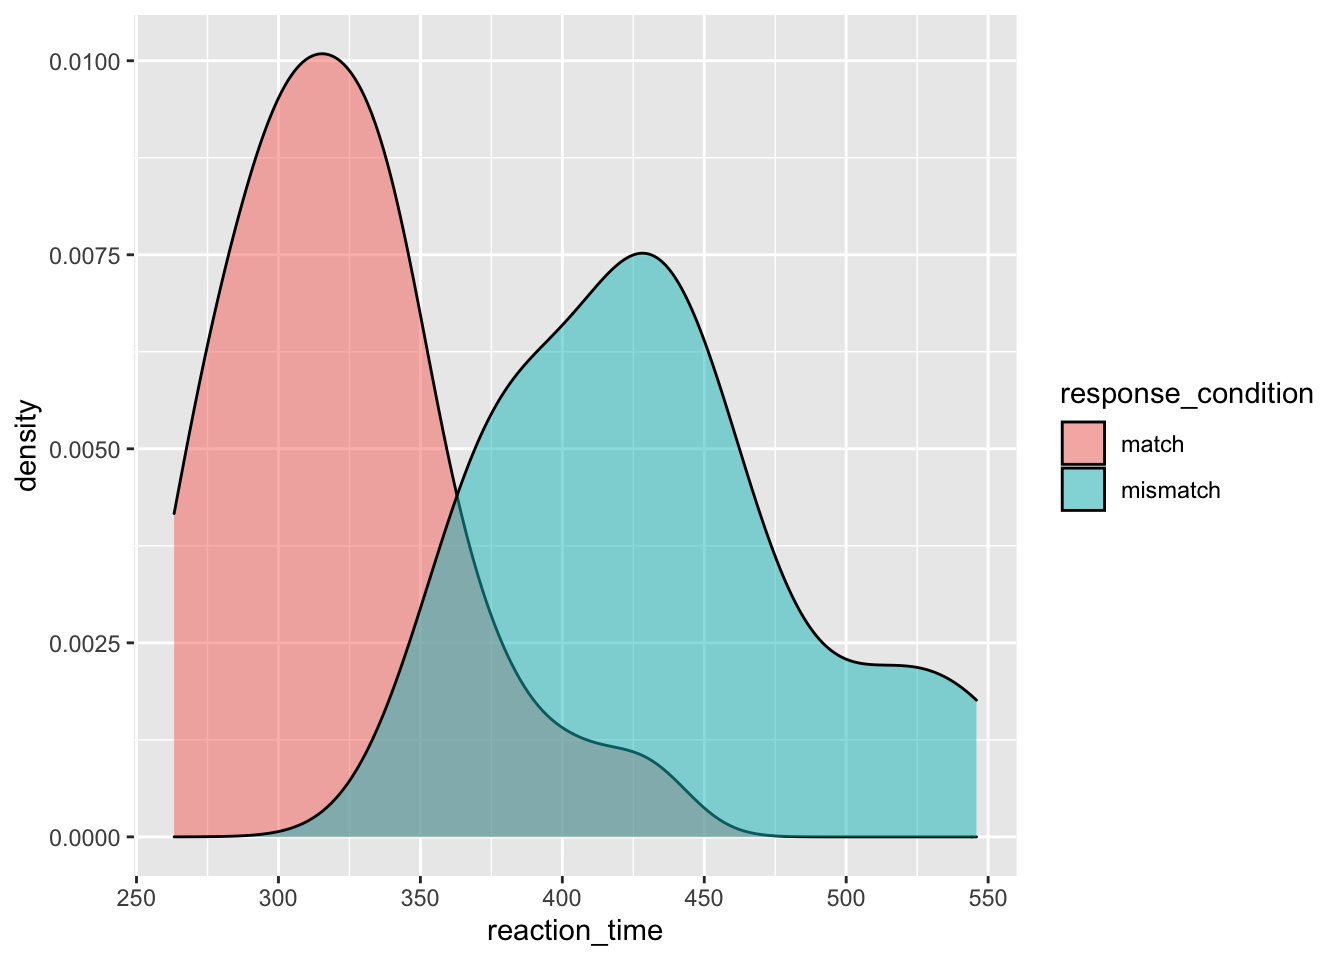
\includegraphics{r4psych_files/figure-latex/3_density_plot_boring-1.pdf}

You already know how to change the colours of your aesthetics across all conditions and split by condition, so now we'll look at other ways to improve the plot.

In this version of the plot, we use the same code as before, but we add labels to the axes using \texttt{labs()}, assigning a nicer looking version of our variables to the x and y axes.

Additionally, we change the scale of the x-axis using the \texttt{scale\_x\_continuous} function. To this function, we pass the \textbf{limits} that we want for our axis (between 200 and 600ms), and we identify the breaks, or where we want the ticks along the axis. We pass another function that we learned in the Lesson One, called \texttt{seq()}. This sets up a sequence of numbers for us without us having to type them all out. Here, it goes \texttt{from} 200 \texttt{to} 600 \texttt{by} ticks every 100ms; as a result, our axis gets labels of 200, 300, 400, 500, and 600.

On top of this, we also improved the label for our legend using the \texttt{guides()} function. As our legend is only there to identify different parts of the graph with a different colour (from \texttt{fill\ =\ response\_condition} in \texttt{aes()}), then we have to tell the guide to change the legend that pops up because of the differnt coloured parts of the plot. So, we change our guide, and change the legend that comes up because of the change in colour (\texttt{guides(fill\ =\ guide\_legend())}) and within the guide legend, we change the title (\texttt{title\ =\ "Response\ Condition"}. I know this sounds like a lot to take in, and you're very likely to forget how this works (I do all the time), but hopefully you can get a grip of it by seeing it in action.

Finally, we've changed the theme of our plot to \texttt{theme\_bw()}. This is one of many inbuilt themes in ggplot2, but I find it one of the cleanest.

\begin{Shaded}
\begin{Highlighting}[]
\FunctionTok{ggplot}\NormalTok{(}\AttributeTok{data =}\NormalTok{ rt\_data, }
       \AttributeTok{mapping =} \FunctionTok{aes}\NormalTok{(}\AttributeTok{x =}\NormalTok{ reaction\_time, }
                     \AttributeTok{fill =}\NormalTok{ response\_condition}
\NormalTok{                     )}
\NormalTok{       ) }\SpecialCharTok{+}
  \FunctionTok{geom\_density}\NormalTok{(}\AttributeTok{alpha =} \FloatTok{0.5}\NormalTok{) }\SpecialCharTok{+}
  \FunctionTok{labs}\NormalTok{(}\AttributeTok{x =} \StringTok{"Reaction Time (ms)"}\NormalTok{, }
       \AttributeTok{y =} \StringTok{"Density"}
\NormalTok{       ) }\SpecialCharTok{+}
  \FunctionTok{scale\_x\_continuous}\NormalTok{(}\AttributeTok{limits =} \FunctionTok{c}\NormalTok{(}\DecValTok{200}\NormalTok{, }\DecValTok{600}\NormalTok{), }
                     \AttributeTok{breaks =} \FunctionTok{seq}\NormalTok{(}\AttributeTok{from =} \DecValTok{200}\NormalTok{, }
                                  \AttributeTok{to =} \DecValTok{600}\NormalTok{, }
                                  \AttributeTok{by =} \DecValTok{100}
\NormalTok{                                  )}
\NormalTok{                     ) }\SpecialCharTok{+}
  \FunctionTok{guides}\NormalTok{(}\AttributeTok{fill =} \FunctionTok{guide\_legend}\NormalTok{(}\AttributeTok{title =} \StringTok{"Response Condition"}\NormalTok{)) }\SpecialCharTok{+}
  \FunctionTok{theme\_bw}\NormalTok{()}
\end{Highlighting}
\end{Shaded}

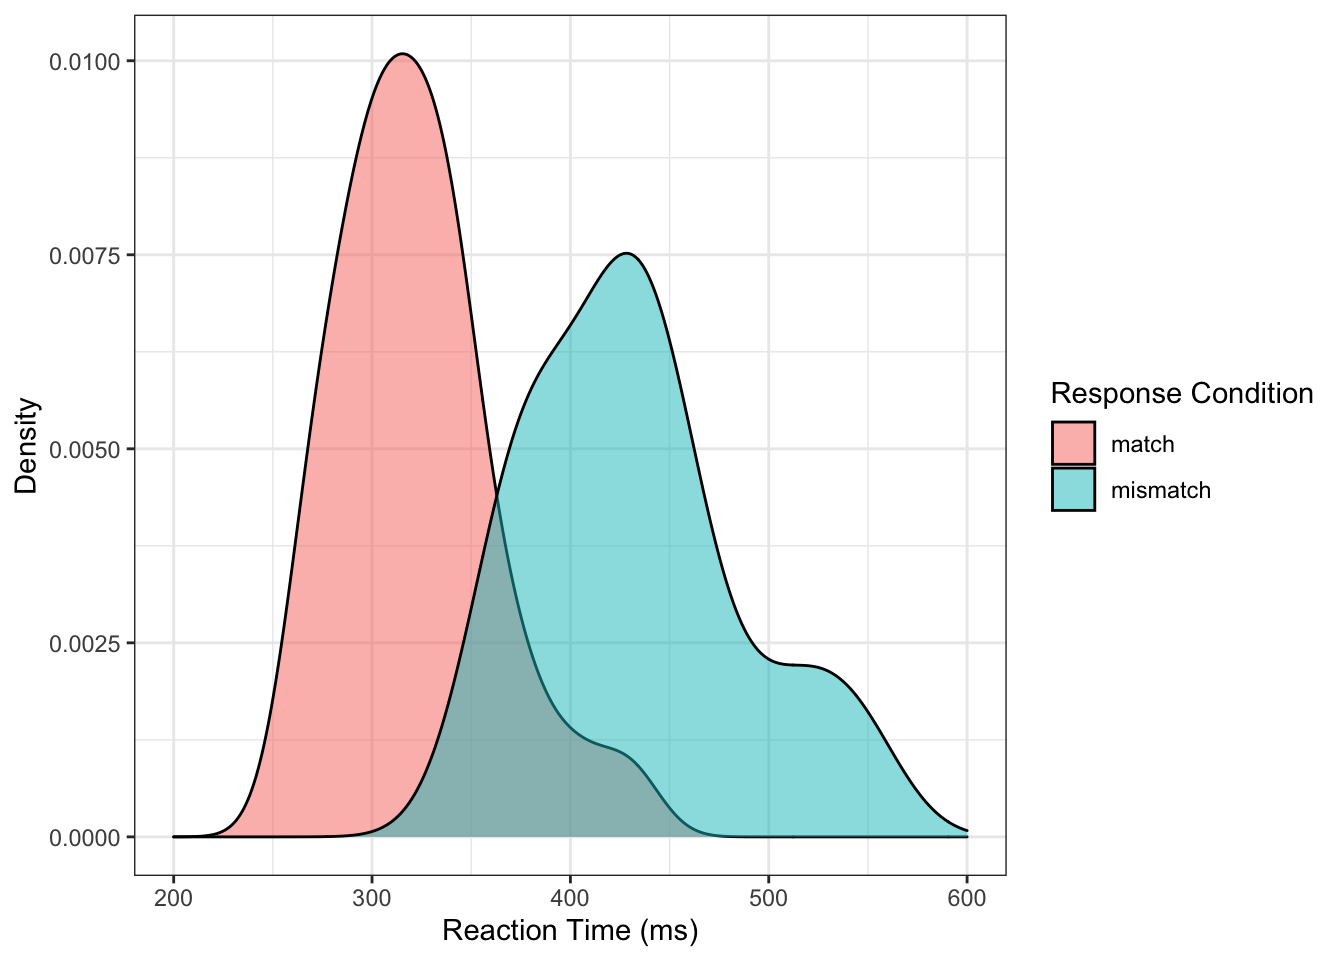
\includegraphics{r4psych_files/figure-latex/3_density_plot_improved-1.pdf}

With the histrogram below, we don't have much new to introduce, expect this time we use \texttt{theme\_classic()} instead of \texttt{theme\_bw()}. This gets rid of the major and minor grid lines from the previous plot, and also keeps only the lines for the axes. However, we added the argument \texttt{expand} to the \texttt{scale\_y\_continuous()} function, and pass this the values 0 and 0. This makes removes the spacing between the plotted elements and the axes. These values simply indicate how much extra space should be added to the top and bottom of the plot.

\begin{Shaded}
\begin{Highlighting}[]
\FunctionTok{ggplot}\NormalTok{(}\AttributeTok{data =}\NormalTok{ rt\_data, }
       \AttributeTok{mapping =} \FunctionTok{aes}\NormalTok{(}\AttributeTok{x =}\NormalTok{ reaction\_time)) }\SpecialCharTok{+}
  \FunctionTok{geom\_histogram}\NormalTok{(}\AttributeTok{binwidth =} \DecValTok{50}\NormalTok{, }
                 \AttributeTok{fill =} \StringTok{"\#bcbddc"}\NormalTok{,}
                 \AttributeTok{colour =} \StringTok{"\#756bb1"}
\NormalTok{                 ) }\SpecialCharTok{+}
  \FunctionTok{scale\_x\_continuous}\NormalTok{(}\AttributeTok{limits =} \FunctionTok{c}\NormalTok{(}\DecValTok{200}\NormalTok{, }\DecValTok{600}\NormalTok{),}
                     \AttributeTok{breaks =} \FunctionTok{seq}\NormalTok{(}\AttributeTok{from =} \DecValTok{200}\NormalTok{, }
                                  \AttributeTok{to =} \DecValTok{600}\NormalTok{, }
                                  \AttributeTok{by =} \DecValTok{25}
\NormalTok{                                  )}
\NormalTok{                     ) }\SpecialCharTok{+}
  \FunctionTok{scale\_y\_continuous}\NormalTok{(}\AttributeTok{expand =} \FunctionTok{c}\NormalTok{(}\DecValTok{0}\NormalTok{, }\DecValTok{0}\NormalTok{)) }\SpecialCharTok{+}
  \FunctionTok{labs}\NormalTok{(}\AttributeTok{x =} \StringTok{"Reaction Time (ms)"}\NormalTok{, }\AttributeTok{y =} \StringTok{"Count"}\NormalTok{) }\SpecialCharTok{+}
  \FunctionTok{theme\_classic}\NormalTok{()}
\end{Highlighting}
\end{Shaded}

\begin{verbatim}
## Warning: Removed 2 rows containing missing values (geom_bar).
\end{verbatim}

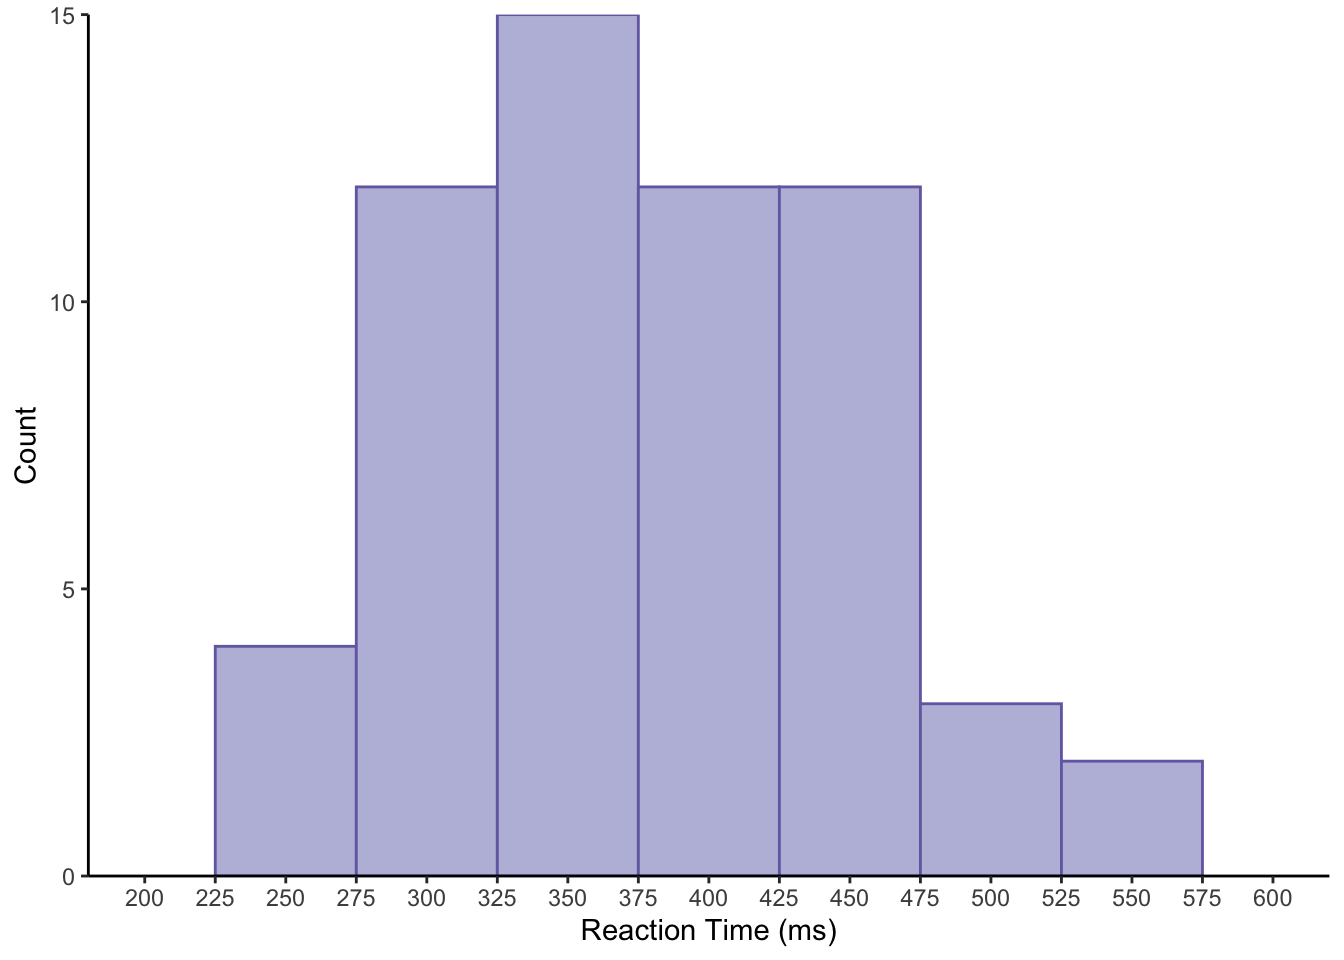
\includegraphics{r4psych_files/figure-latex/3_histogram_plot-1.pdf}

\hypertarget{pirate-plots}{%
\section{Pirate Plots}\label{pirate-plots}}

Now we'll look at a new plot type that takes a bit of extra work to generate; pirate plots. Pirate plots are a great choice of plot for the indecisive. They are essentially the individual points of data, a bar plot, a violin plot, and a confidence interval interval all in one. This way, you get to see the raw, descriptive, and inferential data on one plot!

This is a nice way to show data that are grouped by categories but with a continuous dependent variable.

We could make these ourselves by doing some calculations and combining \texttt{geoms} in ggplot2. Or, we could just install a package from \href{https://github.com/mikabr/ggpirate}{Github} which will do that for us. First, we'll have to install \texttt{devtools} in R which will allow us to install packages from Github. (For packages on CRAN, this isn't necessary, but unfortunately ggpirate isn't on CRAN at the time of writing.)

To install \texttt{devtools} and the \texttt{ggpirate} package, uncomment and run the code below. Then as always, use \texttt{library(ggpirate)} to load the package.

\begin{Shaded}
\begin{Highlighting}[]
\CommentTok{\# install.packages("devtools")}
\CommentTok{\# devtools::install\_github("mikabr/ggpirate")}
\FunctionTok{library}\NormalTok{(ggpirate)}
\end{Highlighting}
\end{Shaded}

Below, we'll make a pirate plot. Note that you only need the first two calls (lines 1-6) to create the plot: The first to set up how you're going to map your data (and the source of your data), and the second to add the \texttt{geom} for the pirate plot itself. We added the aethetics of colour and fill to match our conditions within this call, so the two levels of \texttt{response\_condition} have different colours.

For the additional lines:

\begin{itemize}
\tightlist
\item
  \texttt{labs} allows you to manually change the x and y axis labels
\item
  \texttt{scale\_x\_discrete} allows you to manipulate your x scale. Within this, we change the labels of the columns using \texttt{labels}. We changed them to Impaired (vs.~impaired) and Intact (vs.~intact) for stylisitc reasons.
\item
  \texttt{scale\_y\_continuous} allows you to manipulate your y scale. Here, we set the \texttt{limits}, i.e.~how far to extend our y-axis to between 0 and 600ms. Additionally, we set our \texttt{breaks} to increment in the sequence (\texttt{seq}) from 0 to 600 by 100ms. This way, we've added more granularity to our axis ticks.
\item
  We use \texttt{theme\_bw()} to change to a black and white theme. There are other themes in ggplot2, but this one is nice and clean.
\item
  Next, \texttt{theme} allows you to manually specify other aspects of how your plot should look. Here, we used \texttt{panel.grid.major.x} and set this to nothing (\texttt{element\_blank()}) because we don't need vertical lines in our plot.
\item
  Finally, we define the colour and fill for our plot using manual hex values using the \texttt{scale\_colour\_manual()} and \texttt{scale\_fill\_manual()} functions.
\end{itemize}

\begin{Shaded}
\begin{Highlighting}[]
\FunctionTok{ggplot}\NormalTok{(}\AttributeTok{data =}\NormalTok{ rt\_data, }
       \AttributeTok{mapping =} \FunctionTok{aes}\NormalTok{(}\AttributeTok{x =}\NormalTok{ response\_condition, }
                     \AttributeTok{y =}\NormalTok{ reaction\_time,}
                     \AttributeTok{colour =}\NormalTok{ response\_condition,}
                     \AttributeTok{fill =}\NormalTok{ response\_condition)}
\NormalTok{       ) }\SpecialCharTok{+}
  \FunctionTok{geom\_pirate}\NormalTok{() }\SpecialCharTok{+}
  \FunctionTok{labs}\NormalTok{(}\AttributeTok{x =} \StringTok{"Motor Skill"}\NormalTok{, }\AttributeTok{y =} \StringTok{"Reaction Time (ms)"}\NormalTok{) }\SpecialCharTok{+}
  \FunctionTok{scale\_x\_discrete}\NormalTok{(}\AttributeTok{labels =} \FunctionTok{c}\NormalTok{(}\StringTok{"Impaired"}\NormalTok{, }\StringTok{"Intact"}\NormalTok{)) }\SpecialCharTok{+}
  \FunctionTok{scale\_y\_continuous}\NormalTok{(}\AttributeTok{limits =} \FunctionTok{c}\NormalTok{(}\DecValTok{0}\NormalTok{, }\DecValTok{600}\NormalTok{), }
                     \AttributeTok{breaks =} \FunctionTok{seq}\NormalTok{(}\AttributeTok{from =} \DecValTok{0}\NormalTok{, }\AttributeTok{to =} \DecValTok{600}\NormalTok{, }\AttributeTok{by =} \DecValTok{100}\NormalTok{)}
\NormalTok{                     ) }\SpecialCharTok{+}
  \FunctionTok{theme\_bw}\NormalTok{() }\SpecialCharTok{+}
  \FunctionTok{theme}\NormalTok{(}\AttributeTok{panel.grid.major.x =} \FunctionTok{element\_blank}\NormalTok{()) }\SpecialCharTok{+}
  \FunctionTok{scale\_colour\_manual}\NormalTok{(}\AttributeTok{values =} \FunctionTok{c}\NormalTok{(}\StringTok{"\#af8dc3"}\NormalTok{, }\StringTok{"\#7fbf7b"}\NormalTok{)) }\SpecialCharTok{+}
  \FunctionTok{scale\_fill\_manual}\NormalTok{(}\AttributeTok{values =} \FunctionTok{c}\NormalTok{(}\StringTok{"\#af8dc3"}\NormalTok{, }\StringTok{"\#7fbf7b"}\NormalTok{))}
\end{Highlighting}
\end{Shaded}

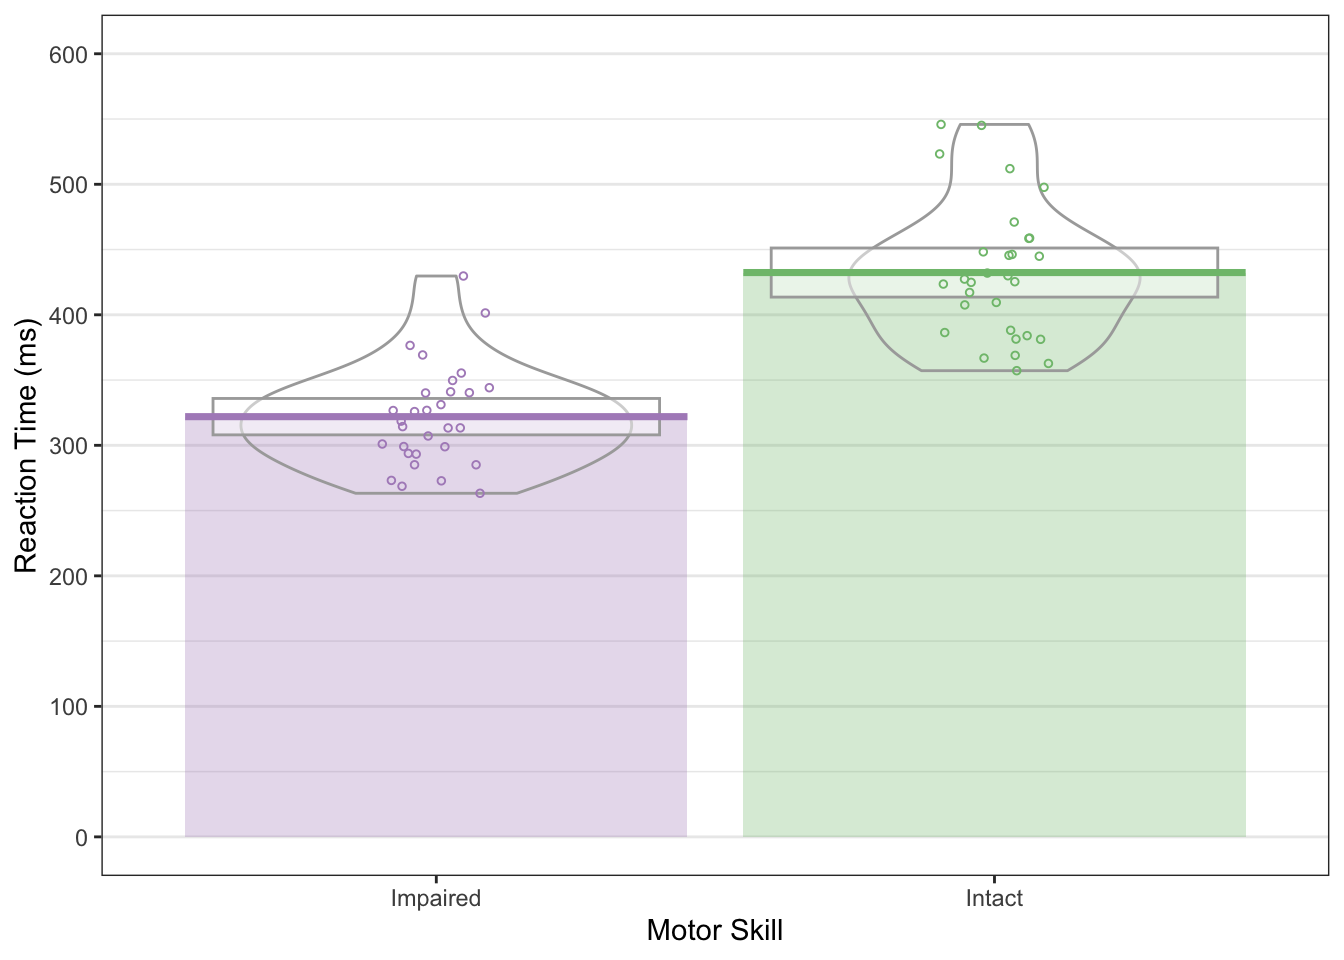
\includegraphics{r4psych_files/figure-latex/3_pirate_plot-1.pdf}

In this plot, we have coloured bars and lines indicating the mean scores, a box representing the 95\% confidence interval assuming a normal sampling distribution, violins indicating density, and the raw data points.

If the 95\% confidence interval between the two groups doesn't overlap, we can be fairly sure there is a significant difference between the groups. So, here we can be fairly certain the two groups differ in reaction times.

\hypertarget{faceting}{%
\section{Faceting}\label{faceting}}

Another useful part of plotting in ggplot2 is that you can make facets of plots, or subplots. This is a good way to display your data if you have multiple categorical variables. Essentially, you'll get a plot for each category in your data.

\hypertarget{facet-wrap}{%
\subsection{Facet Wrap}\label{facet-wrap}}

If you want to create facets from one variable then use \texttt{facet\_wrap()}.

\begin{Shaded}
\begin{Highlighting}[]
\FunctionTok{ggplot}\NormalTok{(}\AttributeTok{data =}\NormalTok{ rt\_data, }\AttributeTok{mapping =} \FunctionTok{aes}\NormalTok{(}\AttributeTok{x =}\NormalTok{ reaction\_time)) }\SpecialCharTok{+}
  \FunctionTok{geom\_histogram}\NormalTok{(}\AttributeTok{binwidth =} \DecValTok{50}\NormalTok{, }
                 \AttributeTok{fill =} \StringTok{"white"}\NormalTok{, }
                 \AttributeTok{colour =} \StringTok{"black"}
\NormalTok{                 ) }\SpecialCharTok{+}
  \FunctionTok{facet\_wrap}\NormalTok{(}\SpecialCharTok{\textasciitilde{}}\NormalTok{ response\_condition)}
\end{Highlighting}
\end{Shaded}

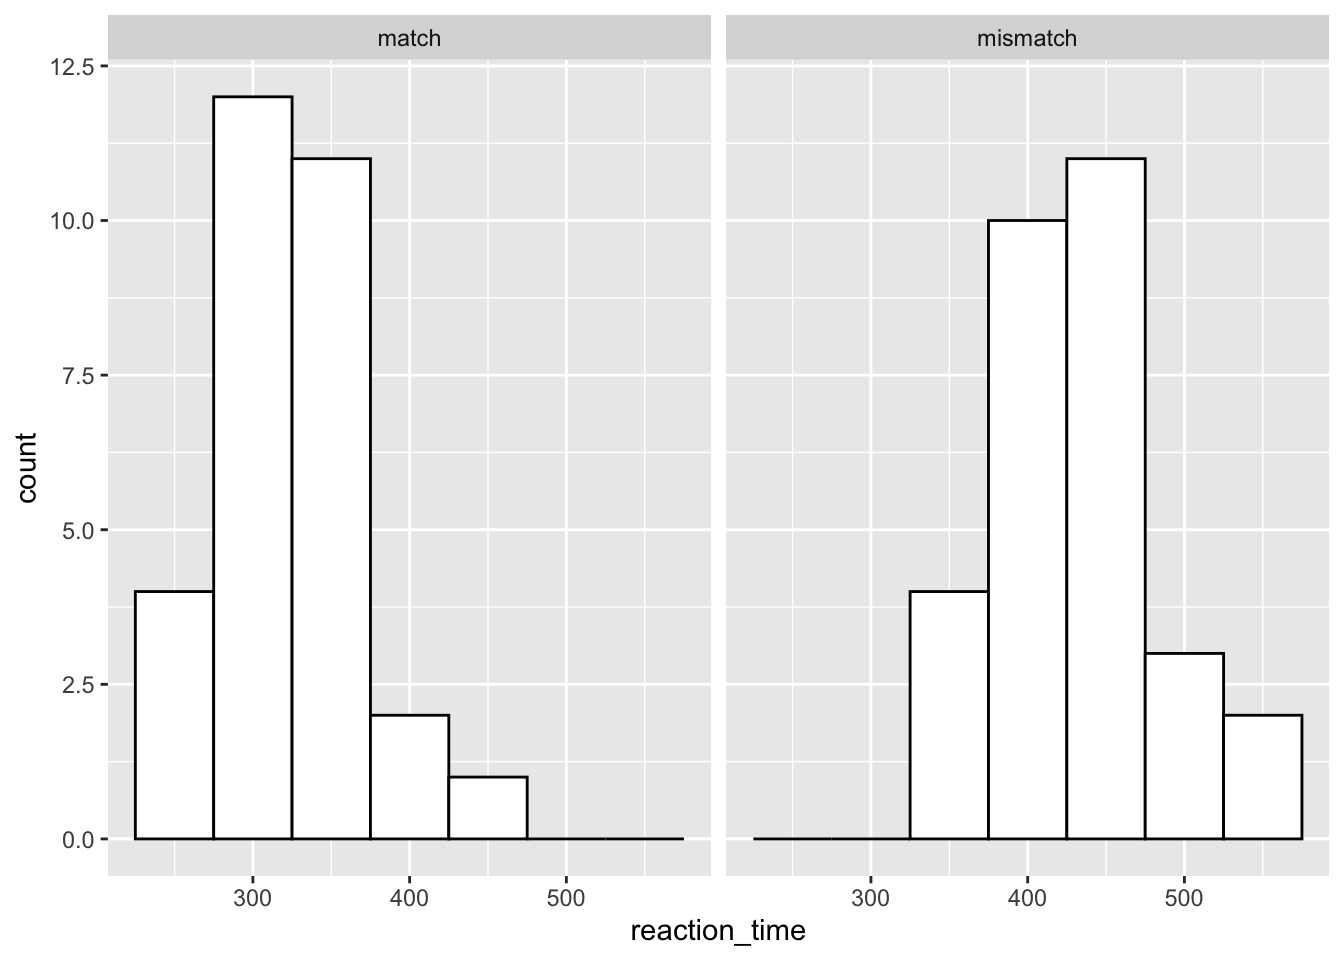
\includegraphics{r4psych_files/figure-latex/3_facet_wrap-1.pdf}

In this plot, we've specified a histogram as we normally would. However, we use \texttt{facet\_wrap()} and a tilde (\texttt{\textasciitilde{}}) to create a formula for how to display our plots. We define our variable with which to split our plots to the right of the \texttt{\textasciitilde{}}, and ggplot automatically plots the two separately at the same time. Notice that we get useful labels at the top of these plots, too.

\hypertarget{facet-grid}{%
\subsection{Facet Grid}\label{facet-grid}}

If we wanted to make a facet by two variables, then we would use \texttt{facet\_grid()} instead. In this case, we just add each variable to either side of the \texttt{\textasciitilde{}} and ggplot will do the splitting for us.

Let's see how this works if we split our data by gender and response condition.

\begin{Shaded}
\begin{Highlighting}[]
\FunctionTok{ggplot}\NormalTok{(}\AttributeTok{data =}\NormalTok{ rt\_data, }\AttributeTok{mapping =} \FunctionTok{aes}\NormalTok{(}\AttributeTok{x =}\NormalTok{ reaction\_time)) }\SpecialCharTok{+}
  \FunctionTok{geom\_histogram}\NormalTok{(}\AttributeTok{binwidth =} \DecValTok{50}\NormalTok{, }
                 \AttributeTok{fill =} \StringTok{"white"}\NormalTok{, }
                 \AttributeTok{colour =} \StringTok{"black"}
\NormalTok{                 ) }\SpecialCharTok{+}
  \FunctionTok{facet\_grid}\NormalTok{(gender }\SpecialCharTok{\textasciitilde{}}\NormalTok{ response\_condition)}
\end{Highlighting}
\end{Shaded}

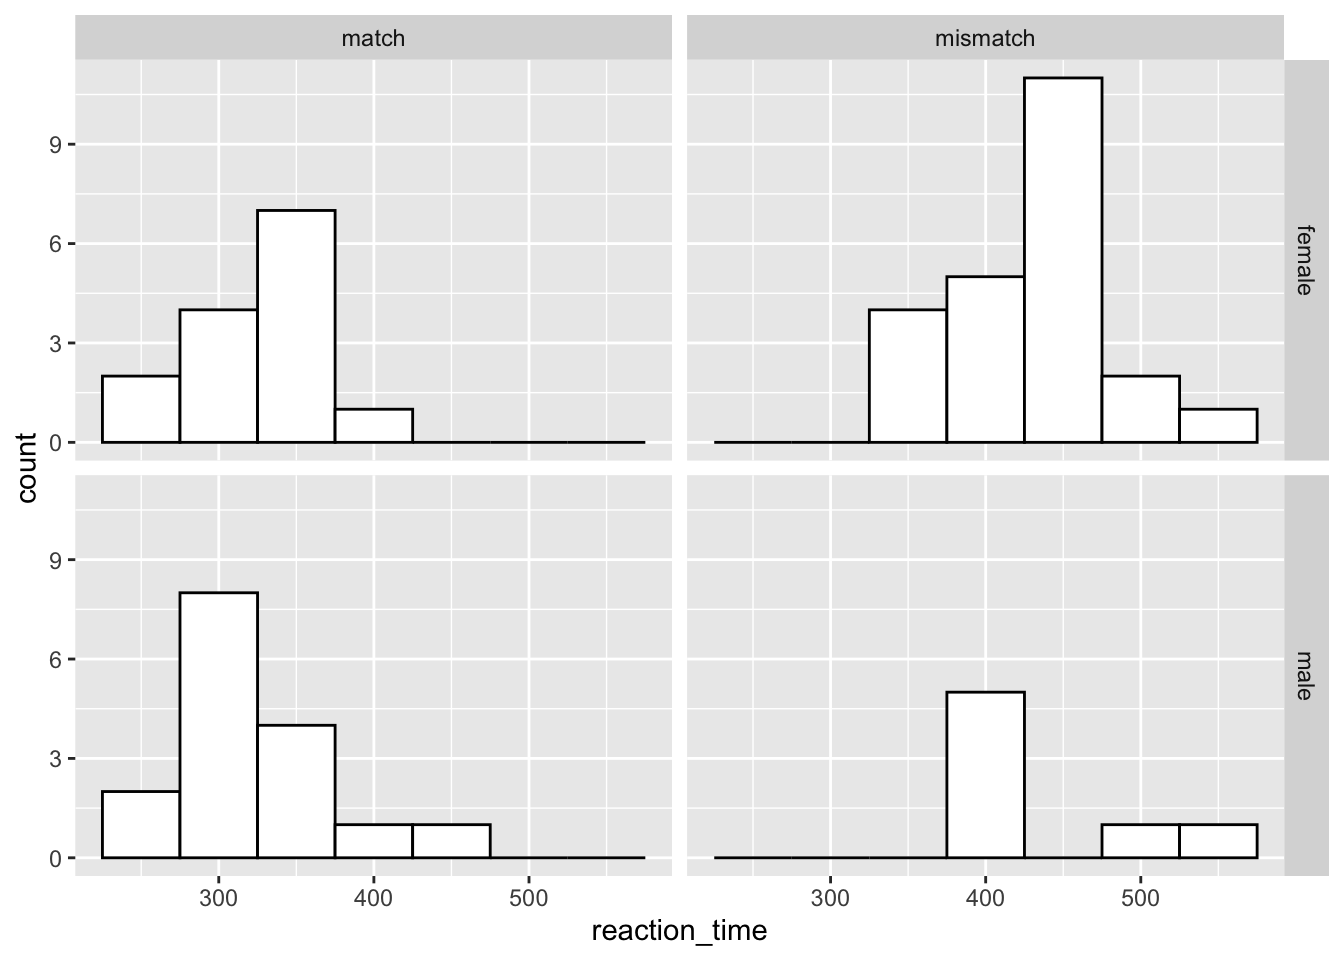
\includegraphics{r4psych_files/figure-latex/3_facet_grid-1.pdf}

The order in which you specify the two variables matters. Try swapping around between \texttt{facet\_wrap(gender\ \textasciitilde{}\ response\_condition)} and \texttt{facet\_wrap(response\_condition\ \textasciitilde{}\ gender)} to see how this works.

\hypertarget{calculating-statisitcs-in-ggplot2}{%
\section{Calculating Statisitcs in ggplot2}\label{calculating-statisitcs-in-ggplot2}}

Sometimes, plotting just the means isn't enough. We saw how useful the 95\% confidence interval from \texttt{ggpirate} is for making inferences about the differences between groups. Nicely, we can get standard errors or confidence intervals around our data points within ggplot for other geoms.

\hypertarget{means-and-error-bars}{%
\subsection{Means and Error Bars}\label{means-and-error-bars}}

Let's say you wanted a bar plot with error bars showing the standard error. You can create this in ggplot using the \texttt{stat\_summary()} function. In the first instance here, we tell it that we want to run the function \texttt{mean} over our data that make up the y-axis; hence \texttt{fun.y\ =\ mean}. We also need to specify which geom we want to return from this.

Try changing the geom to \texttt{point} in the first \texttt{stat\_summary()} call to see what happens when you run this plot with \texttt{geom\ =\ "point"}.

Finally, we ask for another summary, but this time we want an error bar. So, for the geom call we request an error bar. Crucially, the function we require to get this errorbar is \texttt{fun.data\ =\ "mean\_se"}. That's because we need the mean to know where the centre the errorbar, and the standard error to get the limits of the bar. We manually changed the width of the bar to a quarter of the bar size using the \texttt{width} argument to stop ggplot returning super wide error bars.

\begin{Shaded}
\begin{Highlighting}[]
\FunctionTok{ggplot}\NormalTok{(}\AttributeTok{data =}\NormalTok{ rt\_data, }
       \AttributeTok{mapping =} \FunctionTok{aes}\NormalTok{(}
         \AttributeTok{x =}\NormalTok{ response\_condition,}
         \AttributeTok{y =}\NormalTok{ reaction\_time, }
         \AttributeTok{fill =}\NormalTok{ response\_condition}
\NormalTok{         )}
\NormalTok{       ) }\SpecialCharTok{+} 
  \FunctionTok{stat\_summary}\NormalTok{(}\AttributeTok{fun.y =} \StringTok{"mean"}\NormalTok{, }\AttributeTok{geom =} \StringTok{"bar"}\NormalTok{) }\SpecialCharTok{+}
  \FunctionTok{stat\_summary}\NormalTok{(}\AttributeTok{fun.data =} \StringTok{"mean\_se"}\NormalTok{, }\AttributeTok{geom =} \StringTok{"errorbar"}\NormalTok{, }\AttributeTok{width =} \FloatTok{0.25}\NormalTok{)}
\end{Highlighting}
\end{Shaded}

\begin{verbatim}
## Warning: `fun.y` is deprecated. Use `fun` instead.
\end{verbatim}

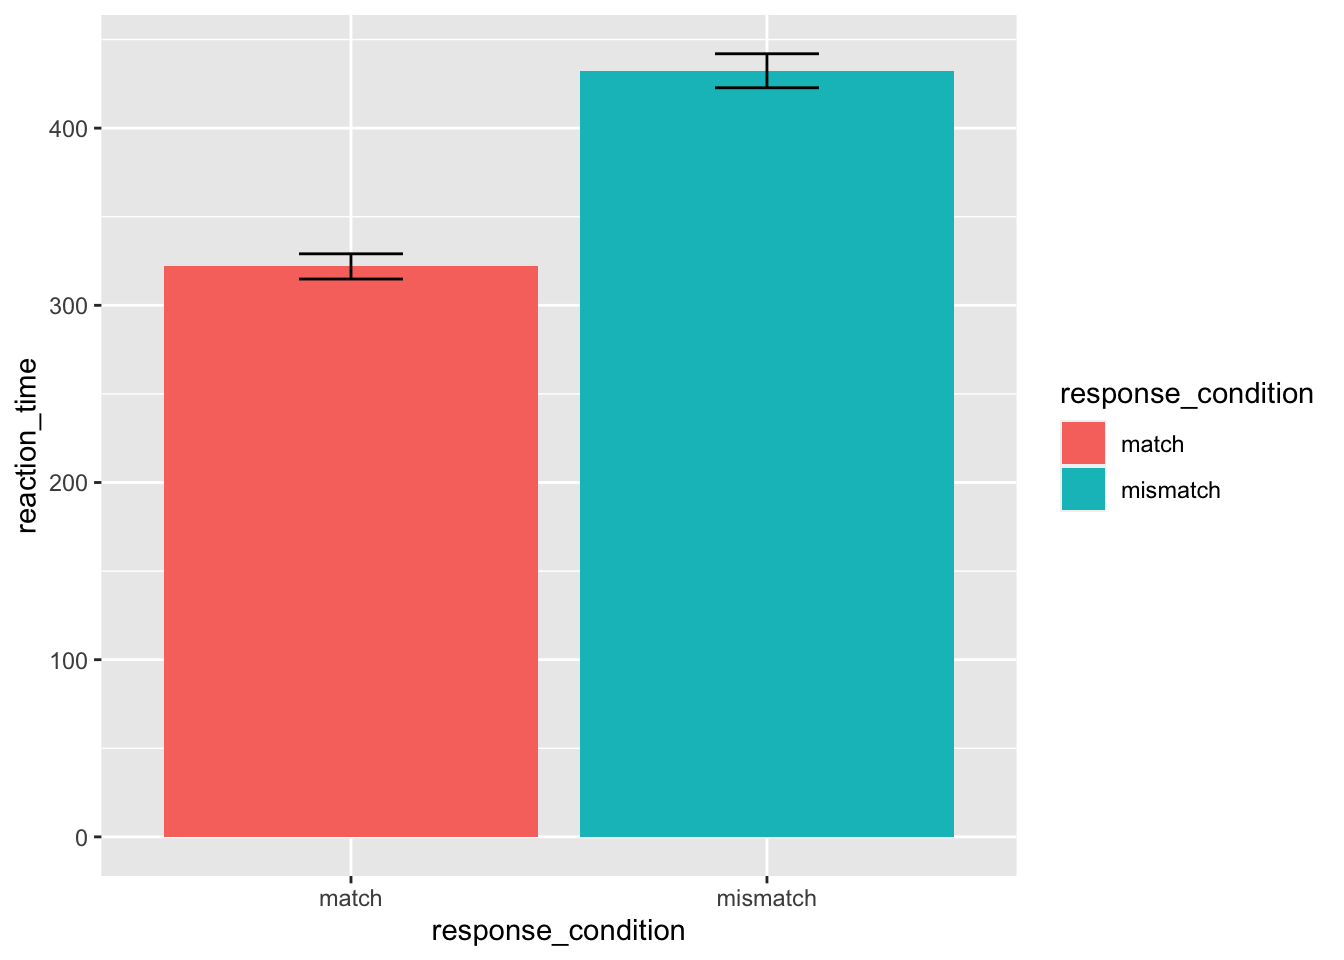
\includegraphics{r4psych_files/figure-latex/3_error_bars-1.pdf}

I don't often use \texttt{stat\_summary} in my own plots, as I often want to know exactly how I've calculated things like the standard error. Doing things by hand allows you to change error bar sizes appropriately for within- and between-subject designs. But, this is useful if you want to create a plot rapidly, or want to avoid the hassle of writing extra code.

\hypertarget{model-fits}{%
\subsection{Model Fits}\label{model-fits}}

Here' we'll switch again to a different data set that has two continuous variables. The \texttt{starwars} data set is useful for this exercise.

We can use the \texttt{geom\_smooth()} function to fit a model to our data. This defaults to a loess method, but we can change this to a linear model (or other alternatives) as in the second plot below. By default, these smoothed plots display a ribbon around the fit which indicates the confidence interval (95\% by default).

\begin{Shaded}
\begin{Highlighting}[]
\CommentTok{\# remove NA and mass above 1000}
\NormalTok{filtered\_starwars }\OtherTok{\textless{}{-}}\NormalTok{ starwars }\SpecialCharTok{\%\textgreater{}\%} 
  \FunctionTok{drop\_na}\NormalTok{(height, mass) }\SpecialCharTok{\%\textgreater{}\%} 
  \FunctionTok{filter}\NormalTok{(mass }\SpecialCharTok{\textless{}} \DecValTok{1000}\NormalTok{)}

\CommentTok{\# plot}
\FunctionTok{ggplot}\NormalTok{(}\AttributeTok{data =}\NormalTok{ filtered\_starwars, }
       \AttributeTok{mapping =} \FunctionTok{aes}\NormalTok{(}\AttributeTok{x =}\NormalTok{ mass, }\AttributeTok{y =}\NormalTok{ height)}
\NormalTok{       ) }\SpecialCharTok{+} 
  \FunctionTok{geom\_point}\NormalTok{() }\SpecialCharTok{+} 
  \FunctionTok{geom\_smooth}\NormalTok{()}
\end{Highlighting}
\end{Shaded}

\begin{verbatim}
## `geom_smooth()` using method = 'loess' and formula 'y ~ x'
\end{verbatim}

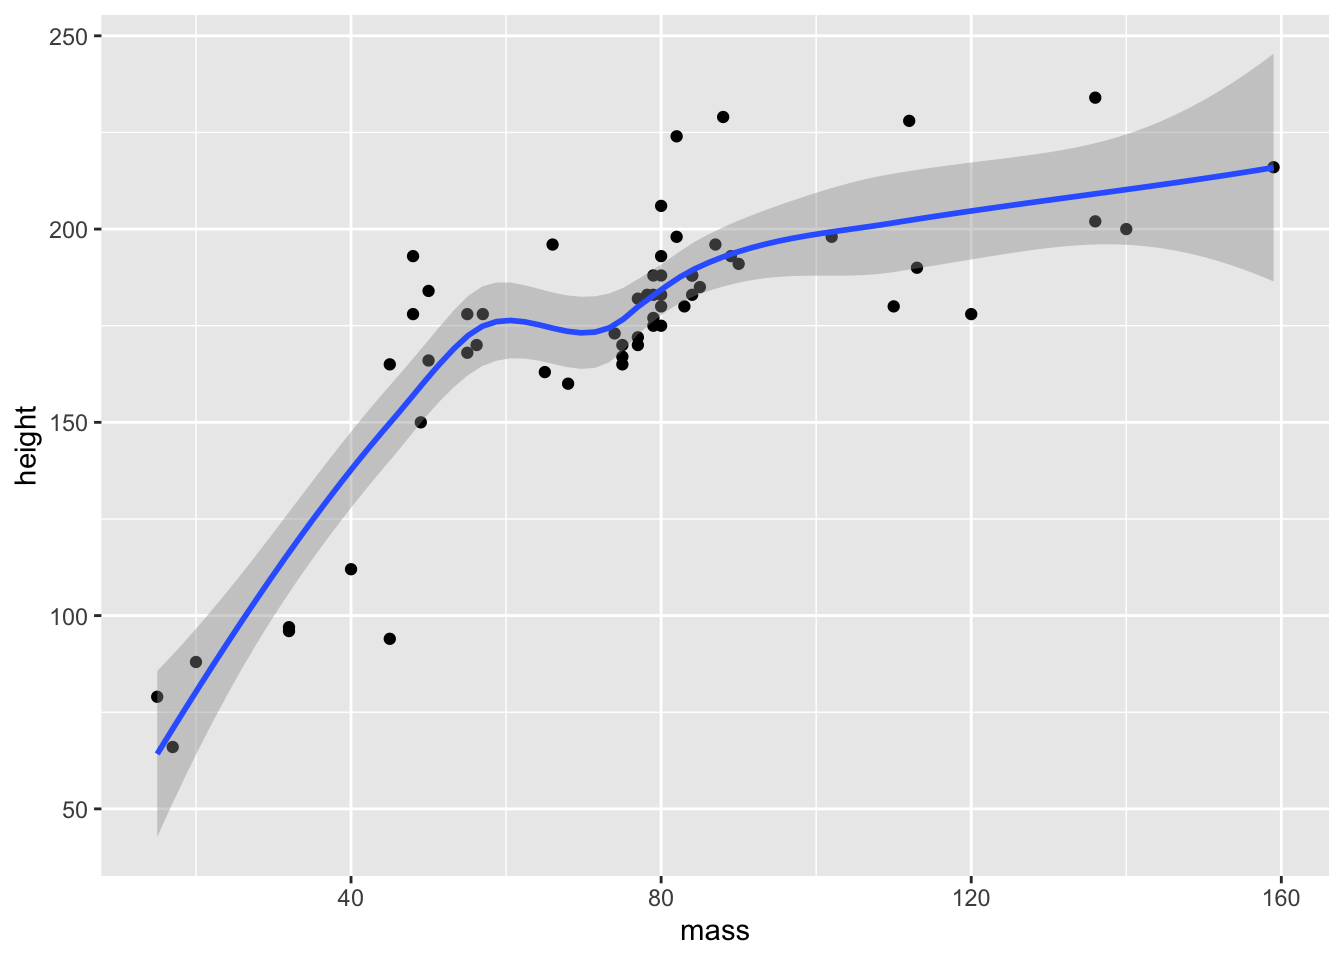
\includegraphics{r4psych_files/figure-latex/3_smooth_starwars-1.pdf}

Next, we'll change the defaults in order to fit a linear model. We do this in the \texttt{geom\_smooth} function, \texttt{method\ =\ "lm"}. We can additionally specify a function, so we can change how we fit the data. Currently, our formula is \texttt{y\ \textasciitilde{}\ x}, which is a regular linear model. We could, however, fit a quadratic function to the data by using \texttt{y\ \textasciitilde{}\ poly(x,\ 2)}. The function \texttt{poly(x,\ 2)} calculates orthogonal polynomials to a certain degree. The first being linear, second quadratic (think curved lines with 1 inflection point), the third cubic (think curved lines with 2 inflection points), etc.. For now, we'll just fit the linear model.

\begin{Shaded}
\begin{Highlighting}[]
\FunctionTok{ggplot}\NormalTok{(}\AttributeTok{data =}\NormalTok{ filtered\_starwars, }
       \AttributeTok{mapping =} \FunctionTok{aes}\NormalTok{(}\AttributeTok{x =}\NormalTok{ mass, }\AttributeTok{y =}\NormalTok{ height)}
\NormalTok{       ) }\SpecialCharTok{+} 
  \FunctionTok{geom\_point}\NormalTok{() }\SpecialCharTok{+} 
  \FunctionTok{geom\_smooth}\NormalTok{(}\AttributeTok{method =} \StringTok{\textquotesingle{}lm\textquotesingle{}}\NormalTok{, }\AttributeTok{formula =}\NormalTok{ y }\SpecialCharTok{\textasciitilde{}}\NormalTok{ x)}
\end{Highlighting}
\end{Shaded}

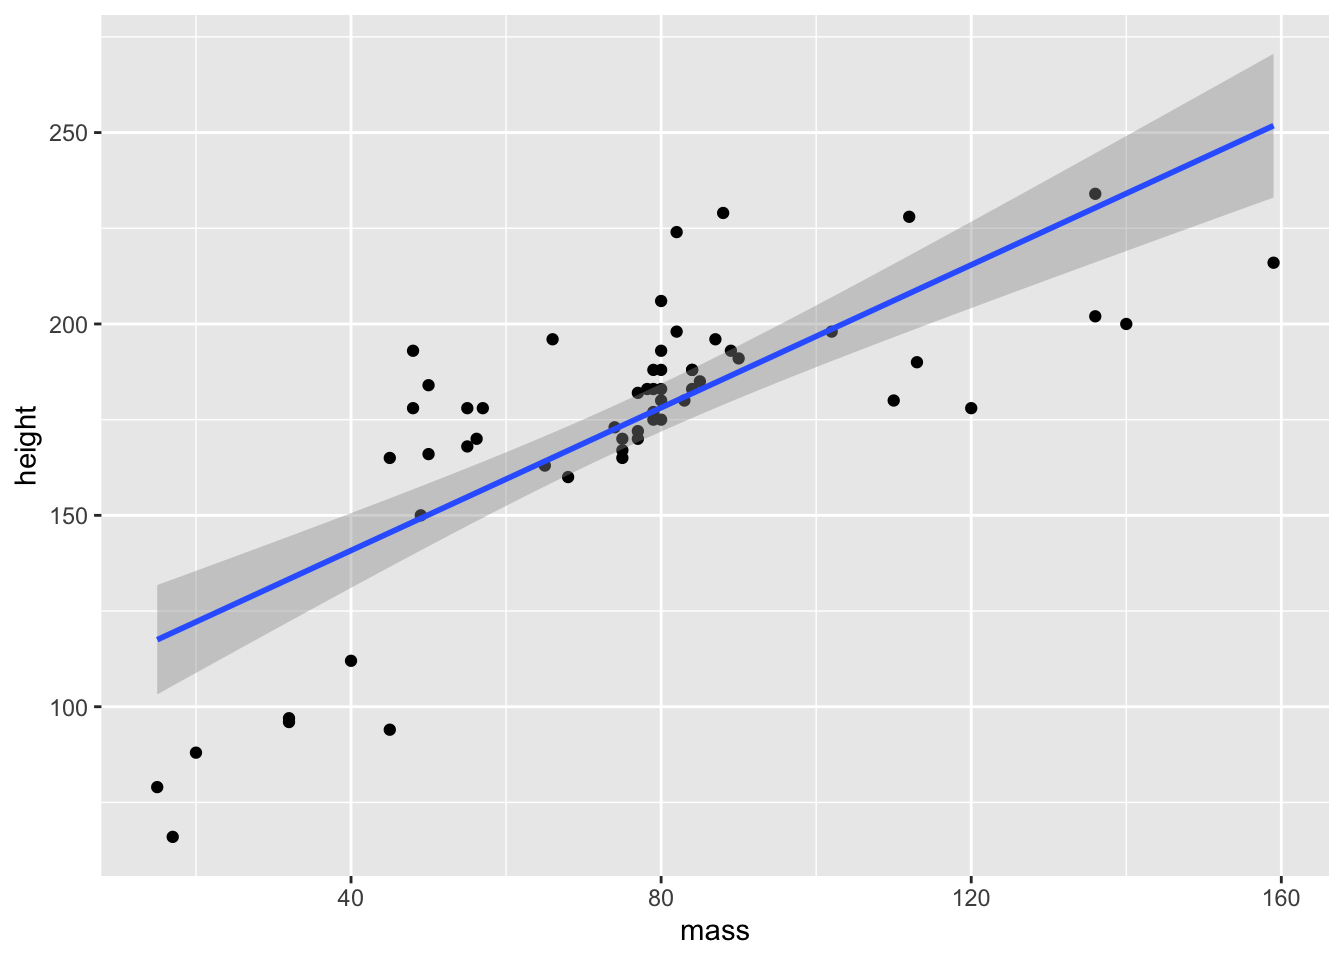
\includegraphics{r4psych_files/figure-latex/3_linear_starwars-1.pdf}

Alternatively, if we have a fitted model saved from our analyses, we can add the fitted line directly using the \texttt{stat\_summary} function. However, this requires some insight into the models fitted, so we'll save this for later classes.

Finally, we'll look at how we can combine these smoothed fits with averages of scores. This is often useful if you're looking at timecourse data and you want to summarise performance across a whole range of participants. We'll also look at adding a few of the graphical flourishes from above to make the plot look really nice.

Next, we'll look at making the point and line points look a little better. For this, we'll use the inbuilt \texttt{ChickWeight} data set from R. This is similar to the \texttt{chickwts} data set from the previous session, but crucially this data is not aggregaged across time. Instead, we have several measurements for the chicks at different time points. This makes this data especially nice for plotting changes over time in our sample.

First, load the data.

\begin{Shaded}
\begin{Highlighting}[]
\FunctionTok{data}\NormalTok{(ChickWeight)}
\end{Highlighting}
\end{Shaded}

Then we can see how the data looks. This data is stored as a data.frame, so we have to be careful when printing it out. We'll use the \texttt{head()} function to get only the first 6 rows of data.

\begin{Shaded}
\begin{Highlighting}[]
\FunctionTok{head}\NormalTok{(ChickWeight)}
\end{Highlighting}
\end{Shaded}

\begin{verbatim}
## Grouped Data: weight ~ Time | Chick
##   weight Time Chick Diet
## 1     42    0     1    1
## 2     51    2     1    1
## 3     59    4     1    1
## 4     64    6     1    1
## 5     76    8     1    1
## 6     93   10     1    1
\end{verbatim}

We have 4 columns:

\begin{itemize}
\tightlist
\item
  weight: out dependent variable, the weight of the chicks
\item
  Time: an independent variable indicating the time point at which a measurement was taken
\item
  Chick: an ID column for each chick
\item
  Diet: an independent variable indicating the diet of the chick
\end{itemize}

Unfortuantely, we only know that there are different diets from the data set, but not what those diets are. We also don't know the units by which weight is measured or by which the measurements were taken.

This is a good lesson in using sensible variable names. If you want yourself and others to understand your data years down the line with little background knowledge of your study, then use informative labels for your data!

We'd expect that as time goes on, chick weights should increase. Also, we might expect that the rate of growth should differ for each diet. As such, we'll plot this together using our data set.

First, we'll plot our chick data, using the \texttt{stat\_summary()} function to plot some mean points for the chick weights, and the \texttt{geom\_smooth()} function to fit a linear model to the data. We'll make sure that the points, lines, and ribbons (indicating the confidence interval) are different colours for each level of the diet factor.

We're going to build up our plot bit by bit, so this time we can same our plot as an object, before returning the object to see the plot.

\begin{Shaded}
\begin{Highlighting}[]
\NormalTok{chick\_time\_plot }\OtherTok{\textless{}{-}} \FunctionTok{ggplot}\NormalTok{(}\AttributeTok{data =}\NormalTok{ ChickWeight, }\CommentTok{\# data}
                          \AttributeTok{mapping =} \FunctionTok{aes}\NormalTok{(}\AttributeTok{x =}\NormalTok{ Time, }\CommentTok{\# x{-}axis}
                                        \AttributeTok{y =}\NormalTok{ weight, }\CommentTok{\# y{-}axis}
                                        \AttributeTok{colour =}\NormalTok{ Diet, }\CommentTok{\# colour ID}
                                        \AttributeTok{fill =}\NormalTok{ Diet }\CommentTok{\# fill ID}
\NormalTok{                                        )}
\NormalTok{                          ) }\SpecialCharTok{+}
  \FunctionTok{stat\_summary}\NormalTok{(}\AttributeTok{fun.y =}\NormalTok{ mean, }\AttributeTok{geom =} \StringTok{"point"}\NormalTok{) }\SpecialCharTok{+} \CommentTok{\# point means}
  \FunctionTok{geom\_smooth}\NormalTok{(}\AttributeTok{method =} \StringTok{\textquotesingle{}lm\textquotesingle{}}\NormalTok{, }\AttributeTok{formula =}\NormalTok{ y }\SpecialCharTok{\textasciitilde{}}\NormalTok{ x) }\CommentTok{\# linear fit}
\end{Highlighting}
\end{Shaded}

\begin{verbatim}
## Warning: `fun.y` is deprecated. Use `fun` instead.
\end{verbatim}

\begin{Shaded}
\begin{Highlighting}[]
\CommentTok{\# return the plot}
\NormalTok{chick\_time\_plot}
\end{Highlighting}
\end{Shaded}

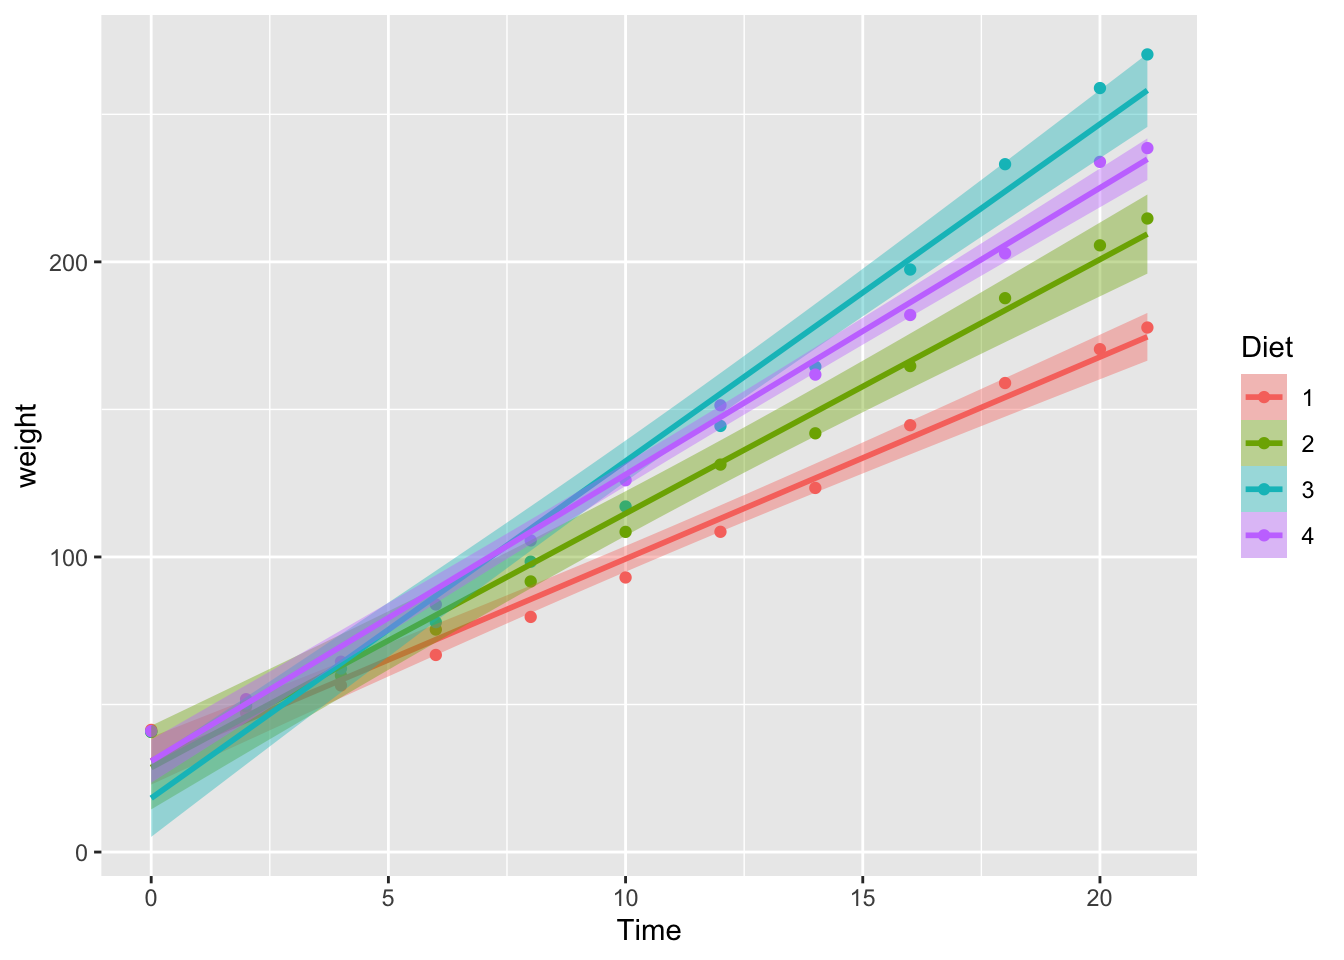
\includegraphics{r4psych_files/figure-latex/3_continuous_data_simple-1.pdf}

We can improve this plot. So, let's add some further information. What if we had a target weight we'd like our chickens to reach over time, and we want to see when each diet pushes chicks over this line?

We can add this information by including a horizontal line using \texttt{geom\_hline()}. We just need to specify where on the y-axis this line should go (\texttt{yintercept}), and which style we want for the line (\texttt{linetype}). We should also add an annotation to the line indicating what it represents. We can do this by using the \texttt{annotate} function, and specifying that we want a text geom. We need to specify the x and y values for where the text lies, and what the text should say.

To add this to our original plot, we'll overwrite the original plot name with itself, plus our additional arguments.

\begin{Shaded}
\begin{Highlighting}[]
\NormalTok{chick\_time\_plot }\OtherTok{\textless{}{-}}\NormalTok{ chick\_time\_plot }\SpecialCharTok{+}
  \FunctionTok{geom\_hline}\NormalTok{(}\AttributeTok{yintercept =} \DecValTok{150}\NormalTok{, }\AttributeTok{linetype =} \DecValTok{2}\NormalTok{) }\SpecialCharTok{+} \CommentTok{\# horizontal line}
  \FunctionTok{annotate}\NormalTok{(}\AttributeTok{geom =} \StringTok{"text"}\NormalTok{, }\AttributeTok{x =} \DecValTok{2}\NormalTok{, }\AttributeTok{y =} \DecValTok{158}\NormalTok{, }\AttributeTok{label =} \StringTok{"Target Weight"}\NormalTok{) }\CommentTok{\# line label}

\CommentTok{\# return the plot}
\NormalTok{chick\_time\_plot}
\end{Highlighting}
\end{Shaded}

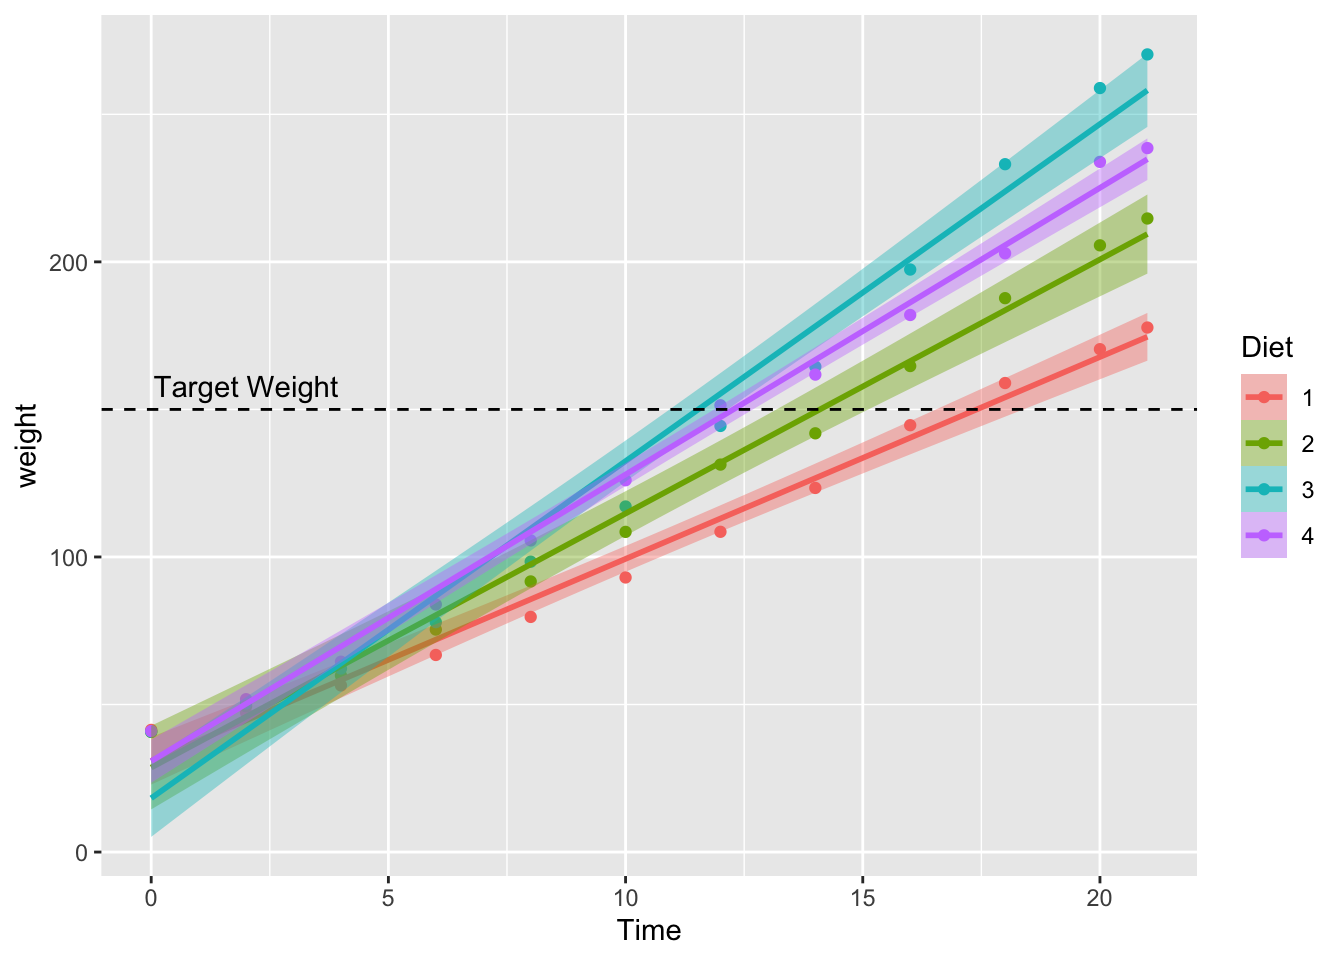
\includegraphics{r4psych_files/figure-latex/3_continuous_data_pretty-1.pdf}

Finally, we can improve the general look of the plot by adding some additional arguments. We'll specify the labels for the x and y axes using the \texttt{labs()} function.

We'll also specify the limits of the y-axis using the \texttt{coord\_cartesian()} function and specifying the minimum and maximum values for the limits of the y-axis.

Next, we'll specify a general basic theme for the plot using the \texttt{theme\_bw()} argument. We'll change a minor detail of this theme, namely the position and style of the legend by specifying additional \texttt{theme()} arguments. This has to come after \texttt{theme\_bw()} so \texttt{theme\_bw()} doesn't overwrite our additional arguments. First, we simply state the x and y locations for the legend by defining the \texttt{legend.position}. Next, we want a black border around our legend, so we do this by changing the \texttt{legend.background}. Here, we set colour (the outline) to black, with a relatively small line size (1), and a solid linetype.

Finally, we can change the title of our legend if we'd like. The original title is quite informative, but it's useful to know how to do this. Here, we use the \texttt{guides} function, and specify both the guide legend title using \texttt{guide\_legend()} for both the \texttt{colour} and \texttt{fill} properties. It's important to do this for both properties as our data is identified by colours on both of these properties. If we just change the title of one of the properties (e.g.~fill), then we'll have two legends!

\begin{Shaded}
\begin{Highlighting}[]
\NormalTok{chick\_time\_plot }\OtherTok{\textless{}{-}}\NormalTok{ chick\_time\_plot }\SpecialCharTok{+}
  \FunctionTok{labs}\NormalTok{(}\AttributeTok{x =} \StringTok{"Trial"}\NormalTok{, }\AttributeTok{y =} \StringTok{"Weight"}\NormalTok{) }\SpecialCharTok{+} \CommentTok{\# axis labels}
  \FunctionTok{coord\_cartesian}\NormalTok{(}\AttributeTok{ylim =} \FunctionTok{c}\NormalTok{(}\DecValTok{0}\NormalTok{, }\DecValTok{300}\NormalTok{)) }\SpecialCharTok{+} \CommentTok{\# range of y{-}axis}
  \FunctionTok{theme\_bw}\NormalTok{() }\SpecialCharTok{+} \CommentTok{\# general theme}
  \FunctionTok{theme}\NormalTok{(}\AttributeTok{legend.position =} \FunctionTok{c}\NormalTok{(}\AttributeTok{x =} \FloatTok{0.15}\NormalTok{, }\AttributeTok{y =} \FloatTok{0.8}\NormalTok{), }\CommentTok{\# position of legend}
        \AttributeTok{legend.background =} \FunctionTok{element\_rect}\NormalTok{(}\AttributeTok{color =} \StringTok{"black"}\NormalTok{,}
                                         \AttributeTok{size =} \DecValTok{1}\NormalTok{,}
                                         \AttributeTok{linetype =} \StringTok{"solid"}
\NormalTok{                                         ) }\CommentTok{\# legend styling}
\NormalTok{  ) }\SpecialCharTok{+}
  \FunctionTok{guides}\NormalTok{(}\AttributeTok{colour =} \FunctionTok{guide\_legend}\NormalTok{(}\StringTok{"Experimental Diet"}\NormalTok{),}
         \AttributeTok{fill =} \FunctionTok{guide\_legend}\NormalTok{(}\StringTok{"Experimental Diet"}\NormalTok{)}
\NormalTok{         ) }\CommentTok{\# legend title}

\CommentTok{\# return the plot}
\NormalTok{chick\_time\_plot}
\end{Highlighting}
\end{Shaded}

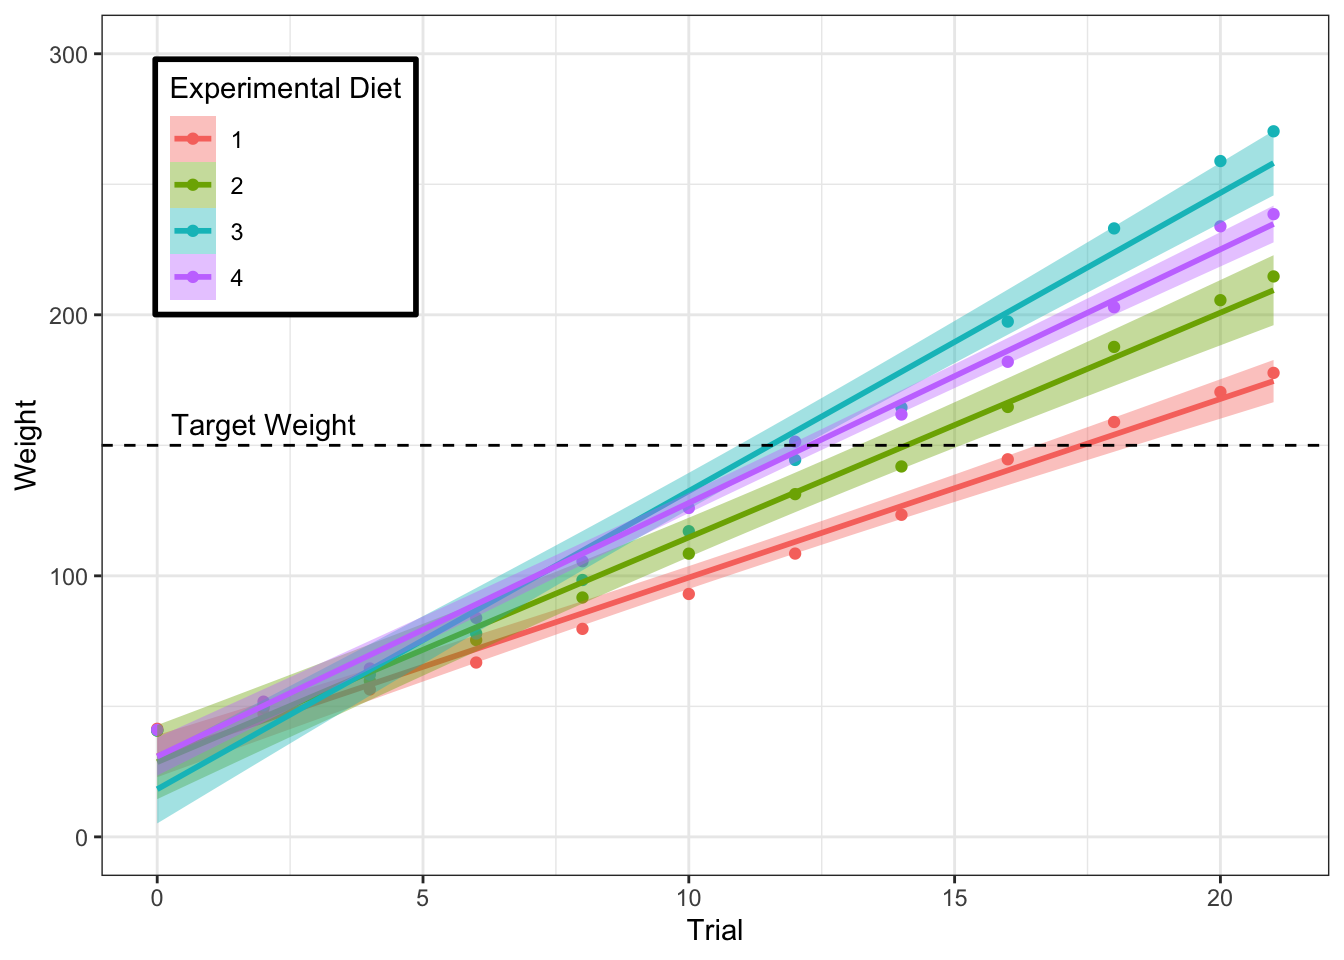
\includegraphics{r4psych_files/figure-latex/3_continuous_data_prettiest-1.pdf}

\hypertarget{combining-plots}{%
\section{Combining Plots}\label{combining-plots}}

Finally, while it's all well and good plotting one model at a time, often if you're writing a paper you want several plots together to save space. You could do this by hand in certain image editing packages, but luckily there's a package for this on CRAN; \texttt{cowplot}. First, we need to install and load the package. Intall this by running the commented out code below. After that, load \texttt{cowplot} each time you want to use it.

\begin{Shaded}
\begin{Highlighting}[]
\CommentTok{\# install.packages("cowplot")}
\FunctionTok{library}\NormalTok{(cowplot) }\CommentTok{\# run this each time}
\end{Highlighting}
\end{Shaded}

In order to stitch two plots together, we need to save our plots as objects so they're available to the R environment. This is the same process we used above for the \texttt{ChickWeight} plots.

If we assign our plotting code to an object, then every time we run the name of the object, we'll get the output of that code back.

For keeping several plots in my environemnt at once, I often save them to an object. In this instance, we'll save a plot of just the points to the name \texttt{point\_plot}. That's because we want to overlay a linear fit and a quadratic fit on this plot separately, but we don't want to type the full code out twice. Instead, we fit the plot of points to \texttt{point\_plot}, then add a linear or quadratic fit by adding the \texttt{geom\_smooth} argument to \texttt{point\_plot} and saving both under new names. We can do this like so:

\begin{Shaded}
\begin{Highlighting}[]
\CommentTok{\# create a plot of points}
\NormalTok{point\_plot }\OtherTok{\textless{}{-}} \FunctionTok{ggplot}\NormalTok{(}\AttributeTok{data =}\NormalTok{ filtered\_starwars, }
                     \AttributeTok{mapping =} \FunctionTok{aes}\NormalTok{(}\AttributeTok{x =}\NormalTok{ mass, }\AttributeTok{y =}\NormalTok{ height)}
\NormalTok{                     ) }\SpecialCharTok{+}
  \FunctionTok{geom\_point}\NormalTok{() }\SpecialCharTok{+}
  \FunctionTok{coord\_cartesian}\NormalTok{(}\AttributeTok{ylim =} \FunctionTok{c}\NormalTok{(}\DecValTok{0}\NormalTok{, }\DecValTok{300}\NormalTok{))}

\CommentTok{\# create a linear plot by adding the fit to the plot of points}
\NormalTok{linear\_plot }\OtherTok{\textless{}{-}}\NormalTok{  point\_plot }\SpecialCharTok{+} 
  \FunctionTok{geom\_smooth}\NormalTok{(}\AttributeTok{method =} \StringTok{\textquotesingle{}lm\textquotesingle{}}\NormalTok{, }\AttributeTok{formula =}\NormalTok{ y }\SpecialCharTok{\textasciitilde{}}\NormalTok{ x)}
\end{Highlighting}
\end{Shaded}

When you do this, you won't automatically see the plot once you run the code unless you run the object assigned to the plot. Let's try this for a quadratic fit of the same data.

\begin{Shaded}
\begin{Highlighting}[]
\CommentTok{\# create a quadratic plot by adding the fit to the plot of points}
\NormalTok{quadratic\_plot }\OtherTok{\textless{}{-}}\NormalTok{ point\_plot }\SpecialCharTok{+} 
  \FunctionTok{geom\_smooth}\NormalTok{(}\AttributeTok{method =} \StringTok{\textquotesingle{}lm\textquotesingle{}}\NormalTok{, }\AttributeTok{formula =}\NormalTok{ y }\SpecialCharTok{\textasciitilde{}} \FunctionTok{poly}\NormalTok{(x, }\DecValTok{2}\NormalTok{)) }\CommentTok{\# fit quadratic}
  
\CommentTok{\# return the plot}
\NormalTok{quadratic\_plot}
\end{Highlighting}
\end{Shaded}

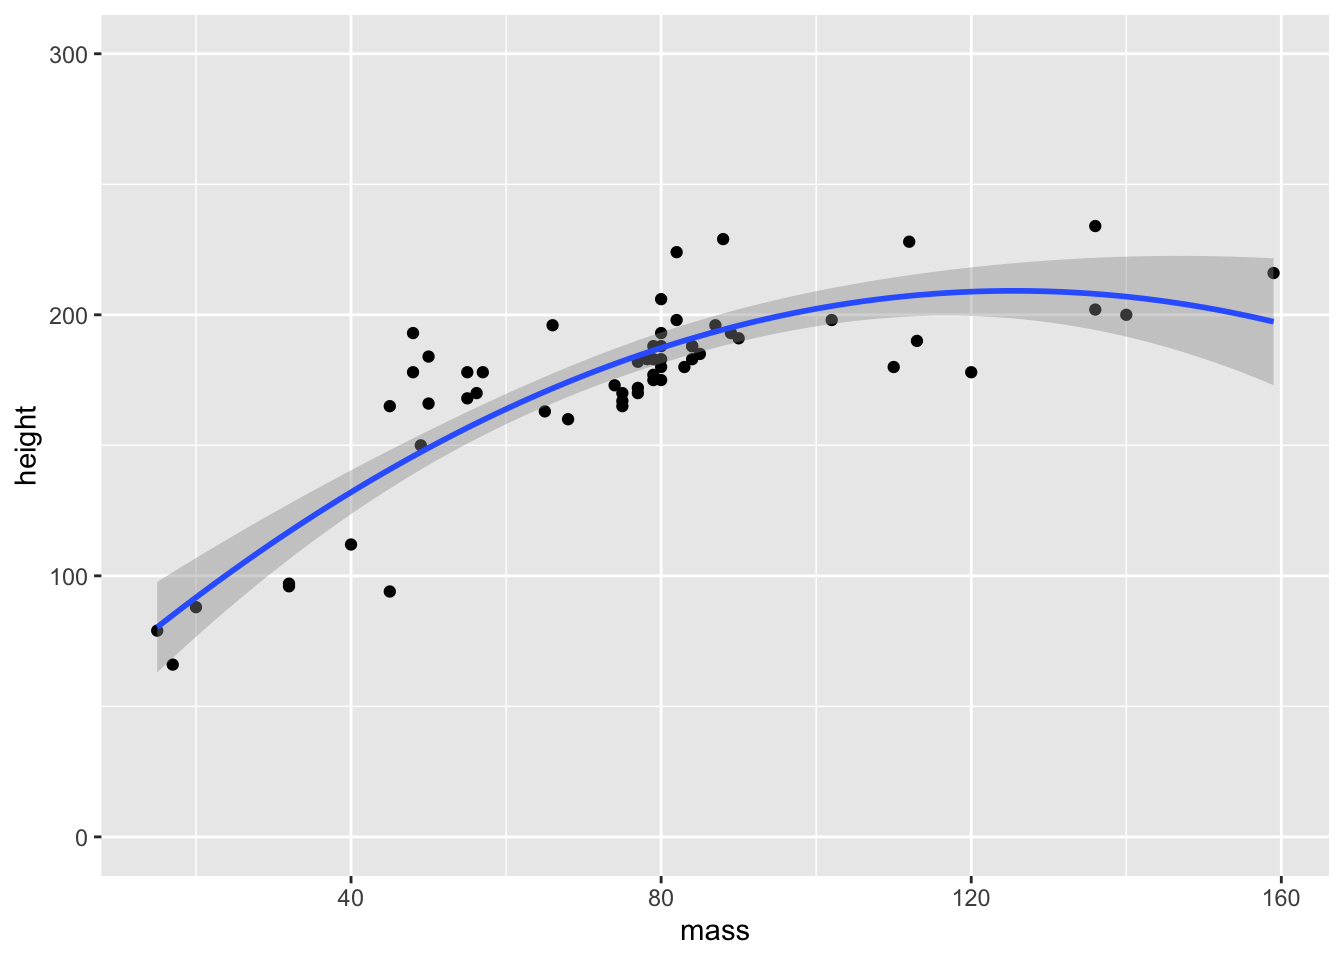
\includegraphics{r4psych_files/figure-latex/3_save_quadratic_plot-1.pdf}

You can see that we've got the quadratic fit and the 95\% confidence interval around this fit from the above code. Why does the plot look different to the base plots in ggplot2? \texttt{cowplot} loads some defaults for all plots outputted by \texttt{ggplot} to save you on typing out your own theme arguments.

Now, we can combine these two plots into a single plot using the new functionalities from \texttt{cowplot}.

\begin{Shaded}
\begin{Highlighting}[]
\NormalTok{combined\_plots }\OtherTok{\textless{}{-}} \FunctionTok{plot\_grid}\NormalTok{(linear\_plot, }
\NormalTok{                            quadratic\_plot, }
                            \AttributeTok{labels =} \FunctionTok{c}\NormalTok{(}\StringTok{"A"}\NormalTok{, }\StringTok{"B"}\NormalTok{), }\CommentTok{\# label plots}
                            \AttributeTok{align =} \StringTok{"h"} \CommentTok{\# align axes}
\NormalTok{                            ) }
\NormalTok{combined\_plots}
\end{Highlighting}
\end{Shaded}

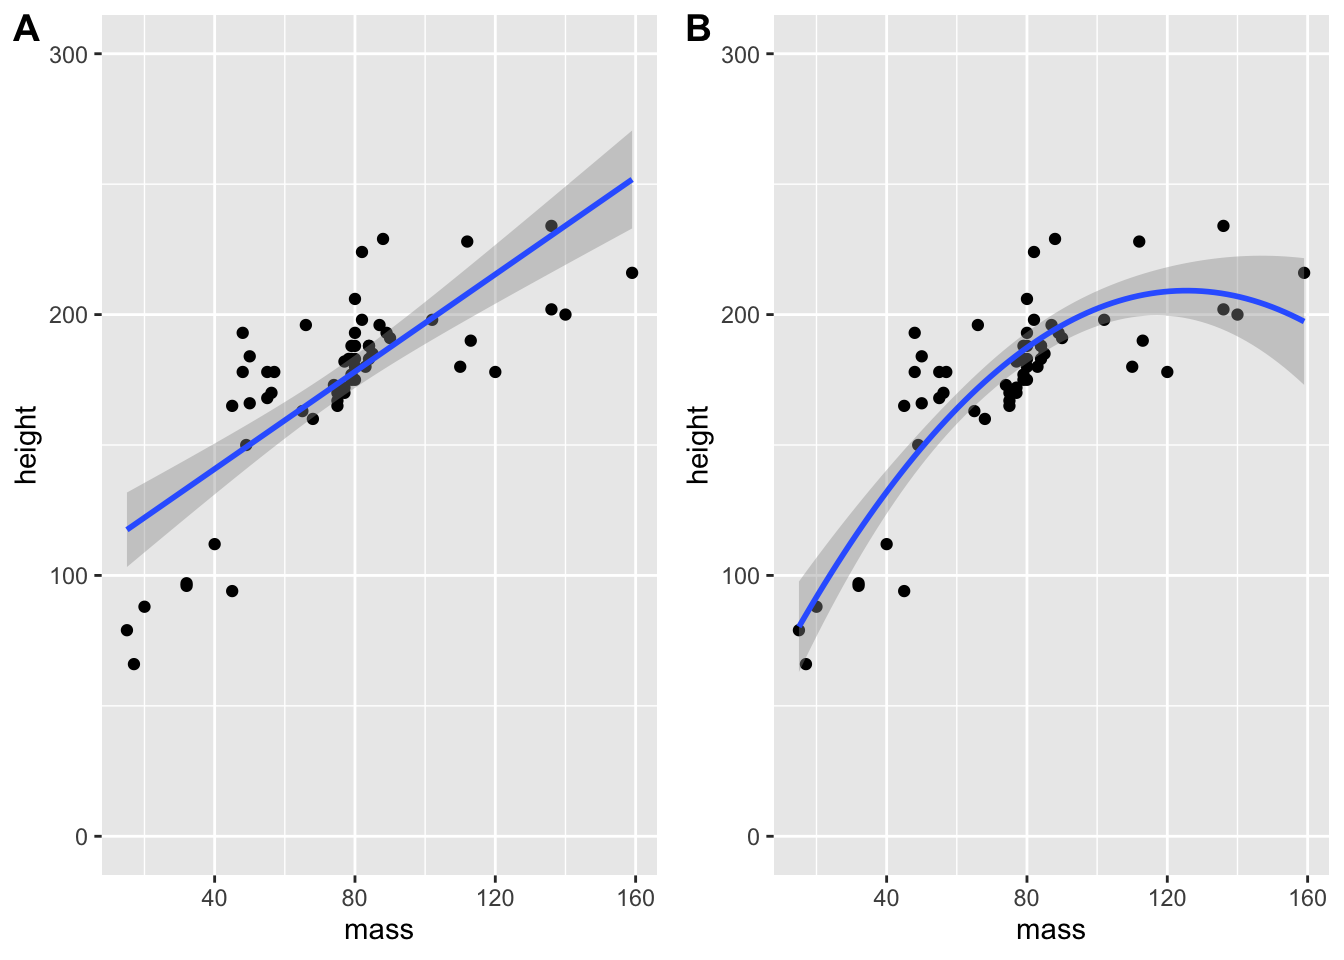
\includegraphics{r4psych_files/figure-latex/3_combine_plots-1.pdf}

What if we want a title for our plots? We first have to define our title with a combination of \texttt{ggdraw()} and \texttt{draw\_label()}. Inside \texttt{draw\_label()} we used a new function, \texttt{paste()} to paste two strings of text together (with a space between the two strings). We could simply input the entire string, but we broke it down into two bits so we don't exceed the 80 character width limit from our style guide!

We further specify a bold \texttt{fontface} in the \texttt{draw\_label()} command outside our pasted title.

Finally, we display the plot by creating a \texttt{plot\_grid()} of our plot and the title in this order so the title displays underneath the plot. We specify that we just want 1 column so the plot and title are stacked together, and we specify the relative heights of the title and plot separately so that the title is smaller than the plot so it doesn't take up an equal amount of space as the plot.

\begin{Shaded}
\begin{Highlighting}[]
\CommentTok{\# create title}
\NormalTok{title }\OtherTok{\textless{}{-}} \FunctionTok{ggdraw}\NormalTok{() }\SpecialCharTok{+} 
  \FunctionTok{draw\_label}\NormalTok{(}\FunctionTok{paste}\NormalTok{(}\StringTok{"Linear (A) and Quadratic"}\NormalTok{,}
                   \StringTok{"(B) fits of Height and Weight"}
\NormalTok{                   ), }
             \AttributeTok{fontface =} \StringTok{"bold"}
\NormalTok{             )}

\CommentTok{\# print plot as a grid}
\NormalTok{combined\_plots }\OtherTok{\textless{}{-}} \FunctionTok{plot\_grid}\NormalTok{(combined\_plots, }
\NormalTok{                            title, }
                            \AttributeTok{ncol =} \DecValTok{1}\NormalTok{, }
                            \AttributeTok{rel\_heights =} \FunctionTok{c}\NormalTok{(}\DecValTok{1}\NormalTok{, }\FloatTok{0.1}\NormalTok{)}
\NormalTok{                            )}

\CommentTok{\# return the combined plots}
\NormalTok{combined\_plots}
\end{Highlighting}
\end{Shaded}

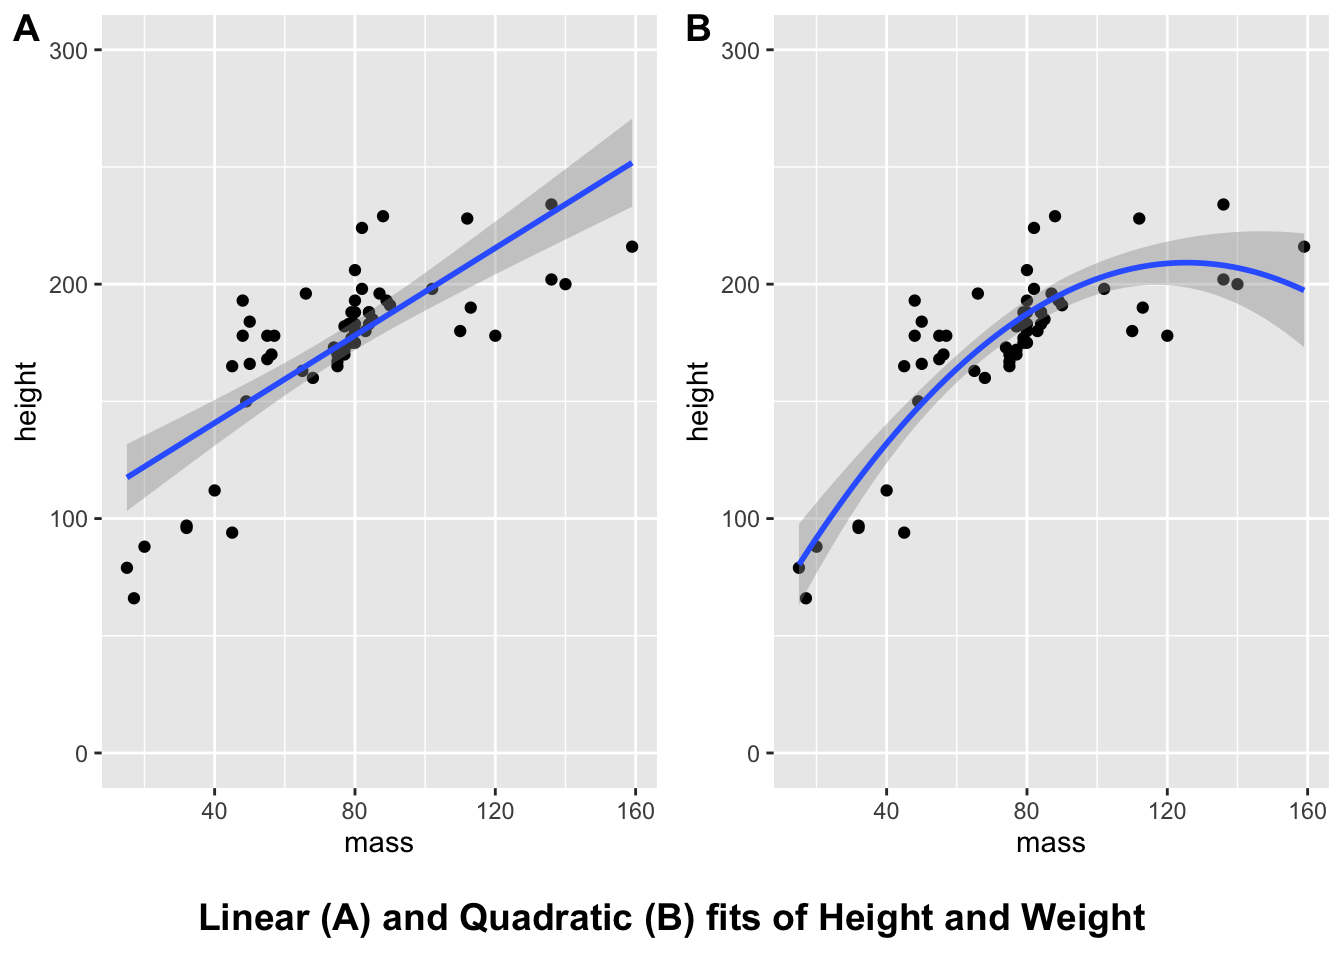
\includegraphics{r4psych_files/figure-latex/3_add_plot_title-1.pdf}

You can find further information on adding joint titles, annotations, etc. in \href{https://htmlpreview.github.io/?https://github.com/wilkelab/cowplot/blob/master/inst/doc/plot_annotations.html}{this article} by Claus O. Wilke.

Note that you can reset the the default styles inherited by cowplot so that your plots return to their defaults with the following code:

\begin{Shaded}
\begin{Highlighting}[]
\FunctionTok{theme\_set}\NormalTok{(}\FunctionTok{theme\_gray}\NormalTok{())}
\end{Highlighting}
\end{Shaded}

\hypertarget{saving-plots}{%
\section{Saving Plots}\label{saving-plots}}

Finally, if you've went to the work of producing a nice plot, then it'll be useful to know how to save it somewhere. To save our combined plot of the linear and quadratic fits, we'll use \texttt{ggsave()}. You can name your plot anything you like, but remember to add a file extension at the end. I've used .png as this format suffers from fewer artifacts when comapred to JPEG, and it's a pretty common filetype.

\begin{Shaded}
\begin{Highlighting}[]
\FunctionTok{ggsave}\NormalTok{(}\AttributeTok{filename =} \StringTok{"outputs/starwars\_mass\_by\_height.png"}\NormalTok{, }
       \AttributeTok{plot =}\NormalTok{ combined\_plots}
\NormalTok{       )}
\end{Highlighting}
\end{Shaded}

You can do a whole bunch of other things with ggplot, like adding vertical and horizontal lines (often useful for identifying chance performance in participants), and annotating plots directly (useful for adding statistics, or commenting on interesting sections of the data). We'll cover these in the exercises, however, as these are just additional flavour to our plots!

\hypertarget{exercises-2}{%
\section{Exercises}\label{exercises-2}}

\hypertarget{main-exercises-1}{%
\subsection{Main Exercises}\label{main-exercises-1}}

If all this complexity hasn't given you \href{https://youtu.be/JidJV1ue1lI}{nausea}, try out the exercises below.

You may have to install the \texttt{languageR} library if you don't have it installed already. We're going to use the \texttt{lexdec} data set from this package. This contains lexical decision times (is this a word or not?) for a range of subjects with different native languages over different words. We also get information on the class of the words (animal or plant), and on the frequency of the words (i.e.~how often they occur in most texts). Finally, our dependent variable is reaction time in the lexical decision task.

Execute the following code to load the data set, clean it, and create an aggregated version of the data set along with some fictional demographics.

\begin{Shaded}
\begin{Highlighting}[]
\CommentTok{\# install.packages("languageR") \# install if needed}
\FunctionTok{library}\NormalTok{(languageR) }\CommentTok{\# load the package containing the lexdec data}

 \CommentTok{\# lexical decision times split by subject and item}
\NormalTok{lex\_dec }\OtherTok{\textless{}{-}}\NormalTok{ lexdec }\SpecialCharTok{\%\textgreater{}\%}
  \FunctionTok{select}\NormalTok{(Subject, NativeLanguage, Trial, Word, Class, Frequency, RT) }\SpecialCharTok{\%\textgreater{}\%}
  \FunctionTok{rename\_all}\NormalTok{(tolower) }\SpecialCharTok{\%\textgreater{}\%}
  \FunctionTok{rename}\NormalTok{(}\AttributeTok{native\_language =}\NormalTok{ nativelanguage, }\AttributeTok{reaction\_time =}\NormalTok{ rt) }\SpecialCharTok{\%\textgreater{}\%}
  \FunctionTok{as.tibble}\NormalTok{()}
\end{Highlighting}
\end{Shaded}

\begin{verbatim}
## Warning: `as.tibble()` was deprecated in tibble 2.0.0.
## Please use `as_tibble()` instead.
## The signature and semantics have changed, see `?as_tibble`.
\end{verbatim}

\begin{Shaded}
\begin{Highlighting}[]
\CommentTok{\# aggregate by items to explore differences in items}
\NormalTok{lex\_dec\_items }\OtherTok{\textless{}{-}}\NormalTok{ lex\_dec }\SpecialCharTok{\%\textgreater{}\%}
  \FunctionTok{group\_by}\NormalTok{(word, class, frequency) }\SpecialCharTok{\%\textgreater{}\%}
  \FunctionTok{summarise}\NormalTok{(}\AttributeTok{mean\_RT =} \FunctionTok{mean}\NormalTok{(reaction\_time),}
            \AttributeTok{sd\_RT =} \FunctionTok{sd}\NormalTok{(reaction\_time)}
\NormalTok{  )}
\end{Highlighting}
\end{Shaded}

\begin{verbatim}
## `summarise()` has grouped output by 'word', 'class'. You
## can override using the `.groups` argument.
\end{verbatim}

\begin{Shaded}
\begin{Highlighting}[]
\CommentTok{\# ensure same values for gender and age columns}
\FunctionTok{set.seed}\NormalTok{(}\DecValTok{1892}\NormalTok{)}

\CommentTok{\# create demographic information}
\CommentTok{\# here, I\textquotesingle{}ve simulated gender and age data}
\NormalTok{lex\_demog }\OtherTok{\textless{}{-}}\NormalTok{ lex\_dec }\SpecialCharTok{\%\textgreater{}\%}
  \FunctionTok{distinct}\NormalTok{(subject, native\_language) }\SpecialCharTok{\%\textgreater{}\%}
  \FunctionTok{mutate}\NormalTok{(}\AttributeTok{age =} \FunctionTok{rnorm}\NormalTok{(}\AttributeTok{n =} \FunctionTok{nrow}\NormalTok{(.), }\AttributeTok{mean =} \DecValTok{35}\NormalTok{, }\AttributeTok{sd =} \DecValTok{7}\NormalTok{),}
         \AttributeTok{gender =} \FunctionTok{sample}\NormalTok{(}\FunctionTok{c}\NormalTok{(}\StringTok{"male"}\NormalTok{, }\StringTok{"female"}\NormalTok{), }
                      \AttributeTok{size =} \FunctionTok{nrow}\NormalTok{(.), }
                      \AttributeTok{replace =} \ConstantTok{TRUE}\NormalTok{)}
\NormalTok{         )}
\end{Highlighting}
\end{Shaded}

Try to solve these questions before resorting to the solutions.

\hypertarget{question-1-2}{%
\subsection{Question 1}\label{question-1-2}}

Let's assume we want to know if the density of the mean reaction times differs across word class within our items.

Using the \texttt{lex\_dec\_items} data set, make a density plot of the word frequency by class. Save this plot as \texttt{lexical\_density}, and output the plot.

\hypertarget{question-2-2}{%
\subsection{Question 2}\label{question-2-2}}

Add a black and white theme to your \texttt{lexical\_density} plot. Next, give the axis labels and legend labels uppercase names. Finally, give your legend title the name Word Class. Assign all of this to a new object \texttt{lexical\_density\_improved}, and output your plot below.

\emph{Note}: To change the legend labels, you need to use both \texttt{scale\_fill\_discrete} and \texttt{scale\_colour\_discrete}. Why do you think this is? Why don't we just use \texttt{scale\_x\_discrete} as we did in class?

\hypertarget{question-3-2}{%
\subsection{Question 3}\label{question-3-2}}

There's some repetition in the code for the plot above. Can you improve your code to remove that?

\hypertarget{question-4-2}{%
\subsection{Question 4}\label{question-4-2}}

Now we want to check the distribution of the reaction times depending on word class and the language spoken by our participants.

Using the \texttt{lex\_dec} data set, create a faceted plot that looks at the density of reaction times. This should be made up of a grid of densities split by native language and word class.

Assign this to the object \texttt{rt\_density} and output your plot.

\hypertarget{question-5-2}{%
\subsection{Question 5}\label{question-5-2}}

Now we want to explore if there's any relationship between the mean reaction time to our items and the frequency of the item.

Using the \texttt{lex\_dec\_items} data set, plot the relationship between word frequency and mean reaction time as a scatter plot. We want a fitted line and points for the mean reaction time.

\hypertarget{question-6-2}{%
\subsection{Question 6}\label{question-6-2}}

Now we want to know how many males and females took part in our experiment.

Using the \texttt{lex\_demog} data set, create a count of the number of males and females who took part in the experiment. Make all text in the plot uppercase, and make the plot theme black and white.

Assign this to the object \texttt{gender\_count} and output your plot.

\hypertarget{question-7-2}{%
\subsection{Question 7}\label{question-7-2}}

What if we want to know the mean age and distribution of ages split by language spoken and gender?

Using the \texttt{lex\_demog} data set, create a pirate plot of the ages by each gender. You can set the colour and fill to gender to have more colourful plot if you'd prefer.

Additionally, we would like these plots split by the native language of the speaker, so facet your plot by native language.

Assign this all to the object \texttt{demographic\_age}, and output your plot.

Can you see how a bar plot of the average ages might be misleading in this instance? Pay particular attention to the male bar for the other language group.

\hypertarget{question-8-2}{%
\subsection{Question 8}\label{question-8-2}}

Next, we want to see the mean (and standard error) of reaction times to words with different word frequencies.

Using the \texttt{lex\_dec} data set, create a scatter plot of the reaction time by word frequency. We would like this split by word class.

\emph{Hint}: Be sure to use the \texttt{stat\_summary} function to get pointranges that represent the mean and standard error.

Assign this to the object \texttt{rt\_pointrange}, and output your plot.

\hypertarget{question-9-2}{%
\subsection{Question 9}\label{question-9-2}}

Finally, we want to show a few of our graphs in one display.

Using the cowplot library, stitch together the plots for question 6, 7, 4, and 8.

Add the labels A-D to identify each plot.

Save these plots under the object \texttt{combined\_plots} and return your combined plots.

\hypertarget{additional-exercise-1}{%
\subsection{Additional Exercise}\label{additional-exercise-1}}

We can improve the combined plots above.

Add a (short) simple title to your combined plots, and save this plot in the outputs folder.

These plots won't look perfect, and you may need to change the font and element sizes. That can be easily achieved, but we won't do that here.

\hypertarget{data-manipulation-1}{%
\chapter{Data Manipulation 1}\label{data-manipulation-1}}

In this chapter we'll look at tidying up and cleaning our data with the \textbf{tidyr} package \citep{R-tidyr} from the tidyverse \citep{R-tidyverse}. We'll also use the \textbf{dplyr} package \citep{R-dplyr} from the tidyverse \citep{R-tidyverse} to join different sets of data together into a useful format for plotting and running analyses.

This data cleaning is an important first step on your way to working with your data, so it's important for you to get acquainted with the different ways your data can be formatted, and how to get it in the format we want.

This chapter, particularly the section on joins, was informed by the \href{https://gupsych.github.io/research_cycle/}{Glasgow University Research Cycle} by Dale Barr and Lisa DeBruine. Please see this resource for further reading.

\hypertarget{getting-started-1}{%
\section{Getting Started}\label{getting-started-1}}

First, we'll load the packages necessary for this class. Nicely, tidyr and dplyr are part of the tidyverse family, so we don't need to load this separately to the other packages in our library.

\begin{Shaded}
\begin{Highlighting}[]
\FunctionTok{library}\NormalTok{(tidyverse)}
\end{Highlighting}
\end{Shaded}

Next, we'll load some data from the \texttt{languageR} library. The data set we'll look at is the \texttt{lexdec} data set, which looks at lexical decision latencies for English nouns from native and non-native speakers of English. If you load this data set from the \texttt{languageR} library then it'll already be in the correct format for us to perform our analyses. So, I've made this data more messy; adding missing values, additional columns that represent more than one source of data, and few extra participants.

On top of this, I've produced a separate data set which stores some (fake) demographic data for the participants. This data set contains information about the participant ID, their gender, age, and any programming languages that they know. Why did I add this last column? Well, sometimes your data contains additional information that isn't important for your current analyses, so it's good to get some experience with filtering our data. (We'll cover filtering data in more detail in Lesson 5.)

\hypertarget{data-formats}{%
\section{Data Formats}\label{data-formats}}

I've saved the data in both \textbf{wide} and \textbf{long} formats.

In \textbf{wide} formats, each row represents one participant, and any information gathered from these participants is stored in a new column. So, let's say we have several items where we gather some data (e.g.~reaction times), here each column will represent an item, and each cell will store a participant's score.

In \textbf{long} formats, each column represents one measurement. Here, we could have a column for participant ID, a column for item number, and a column for reaction times. In this instance, each row should be unique by its combination of our three columns, but IDs (e.g.~participant ID, item ID) will be repeated several times.

\hypertarget{loading-data}{%
\subsection{Loading Data}\label{loading-data}}

Let's load the messy data sets from the csv files in the Lesson 4 \textbf{lesson\_materials} folder to get a better grasp of these formats. We'll get some (scary looking, red) messages when we load the data. That's because we haven't specified how we want each column to be parsed.

\begin{Shaded}
\begin{Highlighting}[]
\NormalTok{demo\_wide }\OtherTok{\textless{}{-}} \FunctionTok{read\_csv}\NormalTok{(}\StringTok{"inputs/lexical\_decision\_demographic\_data\_wide.csv"}\NormalTok{)}
\NormalTok{demo\_long }\OtherTok{\textless{}{-}} \FunctionTok{read\_csv}\NormalTok{(}\StringTok{"inputs/lexical\_decision\_demographic\_data\_long.csv"}\NormalTok{)}
\end{Highlighting}
\end{Shaded}

When we use \texttt{read\_csv()} this function tries to guess the data type contained within any column. Basically, if all the data in a column are numbers, then it'll be parsed as a numeric data type. If even one cell in a column is text, the whole column will be parsed as text. This can cause problems if most of the data are numbers and you want to do some calculations with this column, as you can't add, subract, or divide with text columns!

Often, dates are parsed as datetimes, which allows for some easy calculations for differences in times. But, our completion\_time column was parsed as a character. Why? Because this column contains two datetimes separated by an underscore. It looks like the researchers (me) were too lazy to actually calculate the completion times, and just threw the start and end times togerther into one column!

\hypertarget{wide-and-long-data}{%
\subsection{Wide and Long Data}\label{wide-and-long-data}}

Now we've loaded the data, and understand how R reads data, let's look back at wide and long data formats.

\hypertarget{wide-data}{%
\subsubsection{Wide Data}\label{wide-data}}

In the wide data format, each row is a participant (ID). We have columns representing all of the programming languages reported to be known by the participants. If a participant knows the language, they get a 1 in this column, otherwise they have an NA. We also have several other columns covering other information gathered.

\begin{Shaded}
\begin{Highlighting}[]
\NormalTok{demo\_wide}
\end{Highlighting}
\end{Shaded}

\begin{verbatim}
## # A tibble: 29 x 14
##    ID    `C++` FORTRAN JavaScr~1 Python     R  Ruby LANGU~2 progr~3 gender   age
##    <chr> <dbl>   <dbl>     <dbl>  <dbl> <dbl> <dbl> <chr>   <chr>   <chr>  <dbl>
##  1 22        1       1         1     NA    NA    NA OTHER   FINISH  female    30
##  2 23        1      NA        NA     NA    NA    NA <NA>    no      male      30
##  3 24       NA       1        NA     NA    NA    NA ENGLISH END     female    30
##  4 25        1       1        NA     NA    NA    NA <NA>    ethics  male      18
##  5 26       NA      NA        NA      1    NA     1 english ethics  male      31
##  6 27       NA       1         1     NA    NA    NA ENGLISH END     female    44
##  7 28       NA      NA        NA     NA     1     1 <NA>    ethics  male      23
##  8 29       NA      NA         1     NA    NA    NA english ethics  male      34
##  9 30       NA       1        NA     NA    NA    NA <NA>    <NA>    female    32
## 10 A2        1       1         1     NA    NA    NA English END     female    33
## # ... with 19 more rows, 3 more variables: tester <chr>, funRec <chr>,
## #   completion_time <chr>, and abbreviated variable names 1: JavaScript,
## #   2: LANGUAGE, 3: progress
\end{verbatim}

\hypertarget{long-data}{%
\subsubsection{Long Data}\label{long-data}}

With the long data format, we have each ID for our data in one column, and the measurements for these variables in each cell. The main difference here is that we have a column at the end called computer\_language which simply lists the language each participant knows. This cuts down on the need for redundant columns for a computer language when a participant doesn't know that language. Compare the languages known for participant 22 in this data set and how it's represented in the wide data set.

In order to display this properly, I'll cut out the columns tester, funRec, and completion time, when printing for this website, but you needn't do this in R.

\begin{Shaded}
\begin{Highlighting}[]
\NormalTok{demo\_long}
\end{Highlighting}
\end{Shaded}

\begin{verbatim}
## # A tibble: 54 x 6
##    ID    LANGUAGE progress gender   age computer_language
##    <chr> <chr>    <chr>    <chr>  <dbl> <chr>            
##  1 22    OTHER    FINISH   female    30 C++              
##  2 22    OTHER    FINISH   female    30 FORTRAN          
##  3 22    OTHER    FINISH   female    30 JavaScript       
##  4 23    <NA>     no       male      30 C++              
##  5 24    ENGLISH  END      female    30 FORTRAN          
##  6 25    <NA>     ethics   male      18 C++              
##  7 25    <NA>     ethics   male      18 FORTRAN          
##  8 26    english  ethics   male      31 Python           
##  9 26    english  ethics   male      31 Ruby             
## 10 27    ENGLISH  END      female    44 FORTRAN          
## # ... with 44 more rows
\end{verbatim}

We end up with some repetition here (several rows with the same ID, language, gender, etc.), but each row is unique when we consider all measurements. This is a common data format for raw data, as we'll see next.

\hypertarget{understanding-our-loaded-data}{%
\subsubsection{Understanding our Loaded Data}\label{understanding-our-loaded-data}}

The NA value is important in R; as Hadley Wickham says, it is the evidence of absence. Missing values however are more problematic in that they are the absence of evidence. If you want to indicate missing data, use NA, and not N/A or N\_A etc. as you have to tell R to parse these as NAs.

We also have columns indicating the language known by the participant, their progress in the experiment (i.e.~did they finish it or not?), their gender, age, who tested them and two final columns. The funRec column tells us whether they liked the experiment or not (on a 0-7 scale) and whether they'd recommend the experiment to others (yes/no). Unfortunately, these values are separated by a dash. This is bad practice as each cell should represent one data point, not two. The same can be said for completion time, with the dates and times for starting and ending the experiment separated by an underscore.

\hypertarget{reformatting-data}{%
\section{Reformatting Data}\label{reformatting-data}}

\hypertarget{gathering-data}{%
\subsection{Gathering Data}\label{gathering-data}}

Let's say we want to perform some operations to change how our data looks. What if we want to turn our data from a wide format into long format? We might do this if we want to make a bar plot which counts how many people know each programming language.

To gather data that is spread across several columns, we use the \texttt{gather()} function.

In this function, we have to specify a few things. As always, with our tidyverse functions we need to tell R which data set on which to perform the function.

We have to say what we will call our new column which contains the headings of the columns we want to gather. Here, we call it \texttt{prog\_lang}, and it will contain the column names for each programming language. (Normally, I'd use a more readable name, but I want to show as many columns for this data on the website.)

Next, we need to specify a value, which will contain the numbers from the programming language columns we've gathered together. This will essentially tell us whether or not people know that language or not.

Finally, we need to give the function the columns to gather together. We can do this by name, or by number. Since our programming language columns are all together, from column number 2 to 7, we can just specify the range of \texttt{2:7}.

\begin{Shaded}
\begin{Highlighting}[]
\FunctionTok{gather}\NormalTok{(}\AttributeTok{data =}\NormalTok{ demo\_wide,}
       \AttributeTok{key =}\NormalTok{ prog\_lang,}
       \AttributeTok{value =}\NormalTok{ known,}
       \DecValTok{2}\SpecialCharTok{:}\DecValTok{7}
\NormalTok{       )}
\end{Highlighting}
\end{Shaded}

\begin{verbatim}
## # A tibble: 174 x 8
##    ID    LANGUAGE progress gender   age tester prog_lang known
##    <chr> <chr>    <chr>    <chr>  <dbl> <chr>  <chr>     <dbl>
##  1 22    OTHER    FINISH   female    30 GW     C++           1
##  2 23    <NA>     no       male      30 GW     C++           1
##  3 24    ENGLISH  END      female    30 GW     C++          NA
##  4 25    <NA>     ethics   male      18 GW     C++           1
##  5 26    english  ethics   male      31 GW     C++          NA
##  6 27    ENGLISH  END      female    44 GW     C++          NA
##  7 28    <NA>     ethics   male      23 GW     C++          NA
##  8 29    english  ethics   male      34 GW     C++          NA
##  9 30    <NA>     <NA>     female    32 GW     C++          NA
## 10 A2    English  END      female    33 RHB    C++           1
## # ... with 164 more rows
\end{verbatim}

That worked nicely, but it seems that it's formatted the data so it goes through each programming language alphabetically first, so our IDs are spread all over the data set.

To fix this, we can use another function, called \texttt{arrange}, which takes a data argument and a column by which to arrange the data.

\hypertarget{the-pipe}{%
\subsubsection{The Pipe}\label{the-pipe}}

At this point, I'll introduce you to a new way of writing our commands which is better when we want to apply several functions. Instead of nesting it all together, we can write our commands from left to right, like how we read English text. Here, we can use the pipe \texttt{\%\textgreater{}\%} at the end of a line, which can be read as ``and then do\ldots{}''. Below, we simply give our data.frame, demo\_wide, and use the pipe to apply the gather function. This is the same code as above, just represented in a different way. Read this like, ``take our data, and then, gather the columns together.''

\begin{Shaded}
\begin{Highlighting}[]
\NormalTok{demo\_wide }\SpecialCharTok{\%\textgreater{}\%} 
  \FunctionTok{gather}\NormalTok{(}
    \AttributeTok{key =}\NormalTok{ prog\_lang,}
    \AttributeTok{value =}\NormalTok{ known,}
    \DecValTok{2}\SpecialCharTok{:}\DecValTok{7}
\NormalTok{    )}
\end{Highlighting}
\end{Shaded}

\begin{verbatim}
## # A tibble: 174 x 8
##    ID    LANGUAGE progress gender   age tester prog_lang known
##    <chr> <chr>    <chr>    <chr>  <dbl> <chr>  <chr>     <dbl>
##  1 22    OTHER    FINISH   female    30 GW     C++           1
##  2 23    <NA>     no       male      30 GW     C++           1
##  3 24    ENGLISH  END      female    30 GW     C++          NA
##  4 25    <NA>     ethics   male      18 GW     C++           1
##  5 26    english  ethics   male      31 GW     C++          NA
##  6 27    ENGLISH  END      female    44 GW     C++          NA
##  7 28    <NA>     ethics   male      23 GW     C++          NA
##  8 29    english  ethics   male      34 GW     C++          NA
##  9 30    <NA>     <NA>     female    32 GW     C++          NA
## 10 A2    English  END      female    33 RHB    C++           1
## # ... with 164 more rows
\end{verbatim}

Still, we're left with the same grouping problem, so we can apply another function, \texttt{arrange()} at the end to arrange the data by ID.

\begin{Shaded}
\begin{Highlighting}[]
\NormalTok{demo\_wide }\SpecialCharTok{\%\textgreater{}\%} 
  \FunctionTok{gather}\NormalTok{(}
    \AttributeTok{key =}\NormalTok{ prog\_lang,}
    \AttributeTok{value =}\NormalTok{ known,}
    \DecValTok{2}\SpecialCharTok{:}\DecValTok{7}
\NormalTok{    ) }\SpecialCharTok{\%\textgreater{}\%}
  \FunctionTok{arrange}\NormalTok{(ID)}
\end{Highlighting}
\end{Shaded}

\begin{verbatim}
## # A tibble: 174 x 8
##    ID    LANGUAGE progress gender   age tester prog_lang  known
##    <chr> <chr>    <chr>    <chr>  <dbl> <chr>  <chr>      <dbl>
##  1 22    OTHER    FINISH   female    30 GW     C++            1
##  2 22    OTHER    FINISH   female    30 GW     FORTRAN        1
##  3 22    OTHER    FINISH   female    30 GW     JavaScript     1
##  4 22    OTHER    FINISH   female    30 GW     Python        NA
##  5 22    OTHER    FINISH   female    30 GW     R             NA
##  6 22    OTHER    FINISH   female    30 GW     Ruby          NA
##  7 23    <NA>     no       male      30 GW     C++            1
##  8 23    <NA>     no       male      30 GW     FORTRAN       NA
##  9 23    <NA>     no       male      30 GW     JavaScript    NA
## 10 23    <NA>     no       male      30 GW     Python        NA
## # ... with 164 more rows
\end{verbatim}

This is now in a better format. However, we have a lot of rows with NA in the language, where people don't know that language. This is redundant information. Additionally, the known column is now redundant if we remove the languages people don't know, so we can remove this column too.

We'll save this data under the name demo\_gathered for comparison with the long formatted data set we already loaded.

\begin{Shaded}
\begin{Highlighting}[]
\NormalTok{demo\_gathered }\OtherTok{\textless{}{-}}\NormalTok{ demo\_wide }\SpecialCharTok{\%\textgreater{}\%} 
  \FunctionTok{gather}\NormalTok{(}
    \AttributeTok{key =}\NormalTok{ prog\_lang,}
    \AttributeTok{value =}\NormalTok{ known,}
    \DecValTok{2}\SpecialCharTok{:}\DecValTok{7}\NormalTok{,}
    \AttributeTok{na.rm =} \ConstantTok{TRUE}
\NormalTok{    ) }\SpecialCharTok{\%\textgreater{}\%}
  \FunctionTok{arrange}\NormalTok{(ID) }\SpecialCharTok{\%\textgreater{}\%}
  \FunctionTok{select}\NormalTok{(}\SpecialCharTok{{-}}\NormalTok{known)}
\end{Highlighting}
\end{Shaded}

\begin{Shaded}
\begin{Highlighting}[]
\NormalTok{demo\_gathered}
\end{Highlighting}
\end{Shaded}

\begin{verbatim}
## # A tibble: 54 x 7
##    ID    LANGUAGE progress gender   age tester prog_lang 
##    <chr> <chr>    <chr>    <chr>  <dbl> <chr>  <chr>     
##  1 22    OTHER    FINISH   female    30 GW     C++       
##  2 22    OTHER    FINISH   female    30 GW     FORTRAN   
##  3 22    OTHER    FINISH   female    30 GW     JavaScript
##  4 23    <NA>     no       male      30 GW     C++       
##  5 24    ENGLISH  END      female    30 GW     FORTRAN   
##  6 25    <NA>     ethics   male      18 GW     C++       
##  7 25    <NA>     ethics   male      18 GW     FORTRAN   
##  8 26    english  ethics   male      31 GW     Python    
##  9 26    english  ethics   male      31 GW     Ruby      
## 10 27    ENGLISH  END      female    44 GW     FORTRAN   
## # ... with 44 more rows
\end{verbatim}

We used the argument, \texttt{na.rm\ =\ TRUE} to remove any rows in our value column, known, with an NA. Since we did that, the known column contains all 1s, as the only languages left are the ones people know. So, we used the \texttt{select} function from \textbf{dplyr} to remove the known column. This function is used to select the column you want to keep in your data set. If you provide a column name with the \texttt{-} prefix, this tells R to keep everything except that column; so we drop it from our data set!

\hypertarget{separating-columns}{%
\subsection{Separating Columns}\label{separating-columns}}

In our wide formatted data, we have two columns which store two data points in each cell: funRec has information on whether people found the experiment fun, and whether they'd recommend it to others. Let's split this into separate columns. We just need to supply the name of the column to separate \texttt{col}, and what you want it split into, as a list of the names the columns should take, \texttt{into}.

As in previous examples, I'll remove the middle rows from the data here, but feel free to print them all yourself in R. I've presented the code to do this below.

\emph{Remember, if we want to supply multiple names, we need to concatenate (\texttt{c}) these names together.}

\begin{Shaded}
\begin{Highlighting}[]
\NormalTok{demo\_gathered }\SpecialCharTok{\%\textgreater{}\%}
  \FunctionTok{separate}\NormalTok{(}
    \AttributeTok{col =}\NormalTok{ funRec,}
    \AttributeTok{into =} \FunctionTok{c}\NormalTok{(}\StringTok{"fun"}\NormalTok{, }\StringTok{"recommend"}\NormalTok{)}
\NormalTok{    )}
\end{Highlighting}
\end{Shaded}

\begin{verbatim}
## # A tibble: 54 x 5
##    ID    tester fun   recommend completion_time                        
##    <chr> <chr>  <chr> <chr>     <chr>                                  
##  1 22    GW     7     no        2018-03-22 23:06:11_2018-03-23 00:25:51
##  2 22    GW     7     no        2018-03-22 23:06:11_2018-03-23 00:25:51
##  3 22    GW     7     no        2018-03-22 23:06:11_2018-03-23 00:25:51
##  4 23    GW     6     yes       2018-03-26 00:30:20_2018-03-26 02:15:52
##  5 24    GW     4     yes       2018-03-21 11:09:38_2018-03-21 12:16:28
##  6 25    GW     0     no        2018-03-25 13:03:58_2018-03-25 14:45:25
##  7 25    GW     0     no        2018-03-25 13:03:58_2018-03-25 14:45:25
##  8 26    GW     4     no        2018-03-24 06:46:30_2018-03-24 08:17:29
##  9 26    GW     4     no        2018-03-24 06:46:30_2018-03-24 08:17:29
## 10 27    GW     5     no        2018-03-21 03:23:57_2018-03-21 04:28:01
## # ... with 44 more rows
\end{verbatim}

Take a look at the two new columns. They are both parsed as characters, even though the fun column only contains numbers. We can ask R to convert the data types for the split column during in the separate function using \texttt{convert\ =\ TRUE}.

\begin{Shaded}
\begin{Highlighting}[]
\NormalTok{demo\_gathered }\SpecialCharTok{\%\textgreater{}\%}
  \FunctionTok{separate}\NormalTok{(}
    \AttributeTok{col =}\NormalTok{ funRec,}
    \AttributeTok{into =} \FunctionTok{c}\NormalTok{(}\StringTok{"fun"}\NormalTok{, }\StringTok{"recommend"}\NormalTok{),}
    \AttributeTok{convert =} \ConstantTok{TRUE}
\NormalTok{    )}
\end{Highlighting}
\end{Shaded}

\begin{verbatim}
## # A tibble: 54 x 5
##    ID    tester   fun recommend completion_time                        
##    <chr> <chr>  <int> <chr>     <chr>                                  
##  1 22    GW         7 no        2018-03-22 23:06:11_2018-03-23 00:25:51
##  2 22    GW         7 no        2018-03-22 23:06:11_2018-03-23 00:25:51
##  3 22    GW         7 no        2018-03-22 23:06:11_2018-03-23 00:25:51
##  4 23    GW         6 yes       2018-03-26 00:30:20_2018-03-26 02:15:52
##  5 24    GW         4 yes       2018-03-21 11:09:38_2018-03-21 12:16:28
##  6 25    GW         0 no        2018-03-25 13:03:58_2018-03-25 14:45:25
##  7 25    GW         0 no        2018-03-25 13:03:58_2018-03-25 14:45:25
##  8 26    GW         4 no        2018-03-24 06:46:30_2018-03-24 08:17:29
##  9 26    GW         4 no        2018-03-24 06:46:30_2018-03-24 08:17:29
## 10 27    GW         5 no        2018-03-21 03:23:57_2018-03-21 04:28:01
## # ... with 44 more rows
\end{verbatim}

That looks much better!

\texttt{separate()} is smart enough to know how to separate values if they are split by special characters. Before, we had an underscore in the funRec column, so it split the data by that. If this fails, you can directly specify how the values are separated using the \texttt{sep} argument.

We also wanted to split the completion\_time column. It looks like the first value is the start time, and the second is the end time. So lets separate these together with the funRec column.

\begin{Shaded}
\begin{Highlighting}[]
\NormalTok{demo\_gathered }\SpecialCharTok{\%\textgreater{}\%}
  \FunctionTok{separate}\NormalTok{(}
    \AttributeTok{col =}\NormalTok{ funRec,}
    \AttributeTok{into =} \FunctionTok{c}\NormalTok{(}\StringTok{"fun"}\NormalTok{, }\StringTok{"recommend"}\NormalTok{),}
    \AttributeTok{convert =} \ConstantTok{TRUE}
\NormalTok{    ) }\SpecialCharTok{\%\textgreater{}\%}
  \FunctionTok{separate}\NormalTok{(}
    \AttributeTok{col =}\NormalTok{ completion\_time,}
    \AttributeTok{into =} \FunctionTok{c}\NormalTok{(}\StringTok{"start\_time"}\NormalTok{, }\StringTok{"end\_time"}\NormalTok{)}
\NormalTok{    )}
\end{Highlighting}
\end{Shaded}

\begin{verbatim}
## Warning: Expected 2 pieces. Additional pieces discarded in 54 rows [1, 2, 3, 4,
## 5, 6, 7, 8, 9, 10, 11, 12, 13, 14, 15, 16, 17, 18, 19, 20, ...].
\end{verbatim}

\begin{verbatim}
## # A tibble: 54 x 6
##    ID    tester   fun recommend start_time end_time
##    <chr> <chr>  <int> <chr>     <chr>      <chr>   
##  1 22    GW         7 no        2018       03      
##  2 22    GW         7 no        2018       03      
##  3 22    GW         7 no        2018       03      
##  4 23    GW         6 yes       2018       03      
##  5 24    GW         4 yes       2018       03      
##  6 25    GW         0 no        2018       03      
##  7 25    GW         0 no        2018       03      
##  8 26    GW         4 no        2018       03      
##  9 26    GW         4 no        2018       03      
## 10 27    GW         5 no        2018       03      
## # ... with 44 more rows
\end{verbatim}

Oops, it looks like separate struggled to split our completion\_time column correctly. That's because it wants to split at every dash, whitespace, colon, and underscore; pretty much the whole completion\_time column! Let's be more specific and tell \texttt{separate()} to just split the columns at the underscore.

Let's also overwrite our demo\_wide data (assign the new data to the old data name) to use this new format in the next section.

\begin{Shaded}
\begin{Highlighting}[]
\NormalTok{demo\_gathered }\OtherTok{\textless{}{-}}\NormalTok{ demo\_gathered }\SpecialCharTok{\%\textgreater{}\%}
  \FunctionTok{separate}\NormalTok{(}
    \AttributeTok{col =}\NormalTok{ funRec,}
    \AttributeTok{into =} \FunctionTok{c}\NormalTok{(}\StringTok{"fun"}\NormalTok{, }\StringTok{"recommend"}\NormalTok{),}
    \AttributeTok{convert =} \ConstantTok{TRUE}
\NormalTok{    ) }\SpecialCharTok{\%\textgreater{}\%}
  \FunctionTok{separate}\NormalTok{(}
    \AttributeTok{col =}\NormalTok{ completion\_time,}
    \AttributeTok{into =} \FunctionTok{c}\NormalTok{(}\StringTok{"start\_time"}\NormalTok{, }\StringTok{"end\_time"}\NormalTok{),}
    \AttributeTok{sep =} \StringTok{"\_"}
\NormalTok{    )}
\end{Highlighting}
\end{Shaded}

\begin{Shaded}
\begin{Highlighting}[]
\CommentTok{\# see the data}
\NormalTok{demo\_gathered}
\end{Highlighting}
\end{Shaded}

\begin{verbatim}
## # A tibble: 54 x 6
##    ID    tester   fun recommend start_time          end_time           
##    <chr> <chr>  <int> <chr>     <chr>               <chr>              
##  1 22    GW         7 no        2018-03-22 23:06:11 2018-03-23 00:25:51
##  2 22    GW         7 no        2018-03-22 23:06:11 2018-03-23 00:25:51
##  3 22    GW         7 no        2018-03-22 23:06:11 2018-03-23 00:25:51
##  4 23    GW         6 yes       2018-03-26 00:30:20 2018-03-26 02:15:52
##  5 24    GW         4 yes       2018-03-21 11:09:38 2018-03-21 12:16:28
##  6 25    GW         0 no        2018-03-25 13:03:58 2018-03-25 14:45:25
##  7 25    GW         0 no        2018-03-25 13:03:58 2018-03-25 14:45:25
##  8 26    GW         4 no        2018-03-24 06:46:30 2018-03-24 08:17:29
##  9 26    GW         4 no        2018-03-24 06:46:30 2018-03-24 08:17:29
## 10 27    GW         5 no        2018-03-21 03:23:57 2018-03-21 04:28:01
## # ... with 44 more rows
\end{verbatim}

That looks a lot better! Notice that we didn't try to convert the start\_time and end\_time columns as this data type doesn't play nicely with separte. We'll look into how to convert between data types in Lesson 5.

\emph{Note}: If every row doesn't produce the same number of columns, you can control what happens here with the \texttt{extra} argument. We won't cover this, but it's useful to know if you get into problems with \texttt{separate()} because of this issue.

Let's compare our gathered data to the long formatted data we already loaded. It's exactly the same, only we separated the two problematic columns -- funRec and completion\_time -- and we have a different label for the programming languages known (prog\_lang vs.~computer\_language).

\begin{Shaded}
\begin{Highlighting}[]
\FunctionTok{head}\NormalTok{(demo\_gathered)}
\FunctionTok{head}\NormalTok{(demo\_long)}
\end{Highlighting}
\end{Shaded}

\begin{verbatim}
## # A tibble: 6 x 11
##   ID    LANGUAGE progress gender   age tester   fun recommend start_time end_t~1
##   <chr> <chr>    <chr>    <chr>  <dbl> <chr>  <int> <chr>     <chr>      <chr>  
## 1 22    OTHER    FINISH   female    30 GW         7 no        2018-03-2~ 2018-0~
## 2 22    OTHER    FINISH   female    30 GW         7 no        2018-03-2~ 2018-0~
## 3 22    OTHER    FINISH   female    30 GW         7 no        2018-03-2~ 2018-0~
## 4 23    <NA>     no       male      30 GW         6 yes       2018-03-2~ 2018-0~
## 5 24    ENGLISH  END      female    30 GW         4 yes       2018-03-2~ 2018-0~
## 6 25    <NA>     ethics   male      18 GW         0 no        2018-03-2~ 2018-0~
## # ... with 1 more variable: prog_lang <chr>, and abbreviated variable name
## #   1: end_time
\end{verbatim}

\begin{verbatim}
## # A tibble: 6 x 9
##   ID    LANGUAGE progress gender   age tester funRec completion_time     compu~1
##   <chr> <chr>    <chr>    <chr>  <dbl> <chr>  <chr>  <chr>               <chr>  
## 1 22    OTHER    FINISH   female    30 GW     7-no   2018-03-22 23:06:1~ C++    
## 2 22    OTHER    FINISH   female    30 GW     7-no   2018-03-22 23:06:1~ FORTRAN
## 3 22    OTHER    FINISH   female    30 GW     7-no   2018-03-22 23:06:1~ JavaSc~
## 4 23    <NA>     no       male      30 GW     6-yes  2018-03-26 00:30:2~ C++    
## 5 24    ENGLISH  END      female    30 GW     4-yes  2018-03-21 11:09:3~ FORTRAN
## 6 25    <NA>     ethics   male      18 GW     0-no   2018-03-25 13:03:5~ C++    
## # ... with abbreviated variable name 1: computer_language
\end{verbatim}

\hypertarget{spreading-data}{%
\subsection{Spreading Data}\label{spreading-data}}

What if we want to go from long format to wide format? This can be useful if we want to do a paired-samples \emph{t}-test, where we might want the first scores in one column, and the second scores in another. (We'll cover \emph{t}-tests in Lesson 6.)

To make our long data wide, we use the \texttt{spread()} function from tidyr.

To spread our data we need a \texttt{key}, the column containing the values we'd like to make column headers. We then also need a value, indicating the column containing the scores associated with the values. Often, this would be conditions in an experiment and test results.
Our problem here is a little more complex. Remember that we dropped the redundant column telling us whether or not people knew a programming language? Well, we need this back so we have a \texttt{value} column to work from. We'll \textbf{mutate} our data to create this column. To do this, we use the \texttt{mutate()} function from \textbf{dplyr}. (We'll look at this process in detail in Lesson 5.) Here, we just set everything in our new known column to 1 as we know if a language is present in a participant's row, then they know it!

\begin{Shaded}
\begin{Highlighting}[]
\NormalTok{demo\_gathered }\SpecialCharTok{\%\textgreater{}\%} 
  \FunctionTok{mutate}\NormalTok{(}\AttributeTok{known =} \DecValTok{1}\NormalTok{) }\SpecialCharTok{\%\textgreater{}\%}
  \FunctionTok{spread}\NormalTok{(}\AttributeTok{key =}\NormalTok{ prog\_lang, }\AttributeTok{value =}\NormalTok{ known)}
\end{Highlighting}
\end{Shaded}

\begin{verbatim}
## # A tibble: 29 x 11
##    ID      fun recomm~1 start~2 end_t~3 `C++` FORTRAN JavaS~4 Python     R  Ruby
##    <chr> <int> <chr>    <chr>   <chr>   <dbl>   <dbl>   <dbl>  <dbl> <dbl> <dbl>
##  1 22        7 no       2018-0~ 2018-0~     1       1       1     NA    NA    NA
##  2 23        6 yes      2018-0~ 2018-0~     1      NA      NA     NA    NA    NA
##  3 24        4 yes      2018-0~ 2018-0~    NA       1      NA     NA    NA    NA
##  4 25        0 no       2018-0~ 2018-0~     1       1      NA     NA    NA    NA
##  5 26        4 no       2018-0~ 2018-0~    NA      NA      NA      1    NA     1
##  6 27        5 no       2018-0~ 2018-0~    NA       1       1     NA    NA    NA
##  7 28        0 no       2018-0~ 2018-0~    NA      NA      NA     NA     1     1
##  8 29        6 no       2018-0~ 2018-0~    NA      NA       1     NA    NA    NA
##  9 30        1 yes      2018-0~ 2018-0~    NA       1      NA     NA    NA    NA
## 10 A2        4 yes      2018-0~ 2018-0~     1       1       1     NA    NA    NA
## # ... with 19 more rows, and abbreviated variable names 1: recommend,
## #   2: start_time, 3: end_time, 4: JavaScript
\end{verbatim}

Great, that looks exactly the same as our demo\_wide data, only with our nicely split columns.

\emph{Note}: If you have your values spread across several columns, spread will spread by every unique value, so be sure to collapse your values into one column before you do this. You can do this using the \texttt{unite()} function, or pasting values together with \texttt{mutate()}, but we'll cover this more in Lesson 5.

\hypertarget{joins}{%
\section{Joins}\label{joins}}

Finally, we'll look at combining data together from separate tables. This is a common problem when we store demographic information in one data set, and test scores in another. Let's say we're interested in differences in performance by age. To do this, we somehow need to join together the demographic information of age with the correct participant ID in the test data.

Let's load some raw data for the lexical decision times to see how we might join data together from separate data sets.

\begin{Shaded}
\begin{Highlighting}[]
\NormalTok{lexdec\_data }\OtherTok{\textless{}{-}} \FunctionTok{read\_csv}\NormalTok{(}\StringTok{"inputs/lexical\_decision\_raw\_data.csv"}\NormalTok{)}
\end{Highlighting}
\end{Shaded}

To make these examples easier to digest, we'll simply look at a single trial for an individual participant. Again, to do this we'll use some subsetting techniques that we'll go into in more detail in Lesson 5.

\begin{Shaded}
\begin{Highlighting}[]
\CommentTok{\# keep only trials (rows) where the word is ant}
\NormalTok{lexdec\_subset }\OtherTok{\textless{}{-}}\NormalTok{ lexdec\_data }\SpecialCharTok{\%\textgreater{}\%} \FunctionTok{filter}\NormalTok{(word }\SpecialCharTok{==} \StringTok{"ant"}\NormalTok{)}
\end{Highlighting}
\end{Shaded}

How does the data look? We have 26 recorded entries. For two participants, they have missing values (NA) for these trials, indicating that they didn't complete this trial, or the trial wasn't recorded.

\begin{Shaded}
\begin{Highlighting}[]
\NormalTok{lexdec\_subset}
\end{Highlighting}
\end{Shaded}

\begin{verbatim}
## # A tibble: 25 x 9
##    subject trial native_language word  class  frequency length correct    RT
##    <chr>   <dbl> <chr>           <chr> <chr>      <dbl>  <dbl> <chr>   <dbl>
##  1 A1        157 English         ant   animal      5.35      3 correct  876.
##  2 A3         41 Other           ant   animal      5.35      3 correct  607.
##  3 C          86 English         ant   animal      5.35      3 correct  725.
##  4 D         138 Other           ant   animal      5.35      3 correct  628.
##  5 I         105 Other           ant   animal      5.35      3 correct  560.
##  6 J          43 Other           ant   animal      5.35      3 correct  516.
##  7 K         183 English         ant   animal      5.35      3 correct  442.
##  8 M1        171 English         ant   animal      5.35      3 correct  427.
##  9 M2        117 Other           ant   animal      5.35      3 correct  530.
## 10 P         115 Other           ant   animal      5.35      3 correct  533.
## # ... with 15 more rows
\end{verbatim}

This data set contains all the information for our trials, including the data to identify each trial, and what the score was on our dependent variables (correct/incorrect response, reaction time). Here we have the data in a nice format where each column represents a variable, and each cell represents a value for that variable.

Let's look at our demographic data set.

As you can tell, our our data is in a long format. Additionally, it looks like we don't have any record of the language spoken by subject 23. On top of this, we have the cryptically named ``no'' entry in the progress column. I'm guessing this means that they decided to withdraw from the experiment. This means that we have more information on participants than we will have in the lexdec\_subset dataset. The implications of this will become apparent as we try out different joining operations.

\begin{Shaded}
\begin{Highlighting}[]
\NormalTok{demo\_gathered}
\end{Highlighting}
\end{Shaded}

\begin{verbatim}
## # A tibble: 54 x 11
##    ID    LANGUAGE progress gender   age tester   fun recommend start_t~1 end_t~2
##    <chr> <chr>    <chr>    <chr>  <dbl> <chr>  <int> <chr>     <chr>     <chr>  
##  1 22    OTHER    FINISH   female    30 GW         7 no        2018-03-~ 2018-0~
##  2 22    OTHER    FINISH   female    30 GW         7 no        2018-03-~ 2018-0~
##  3 22    OTHER    FINISH   female    30 GW         7 no        2018-03-~ 2018-0~
##  4 23    <NA>     no       male      30 GW         6 yes       2018-03-~ 2018-0~
##  5 24    ENGLISH  END      female    30 GW         4 yes       2018-03-~ 2018-0~
##  6 25    <NA>     ethics   male      18 GW         0 no        2018-03-~ 2018-0~
##  7 25    <NA>     ethics   male      18 GW         0 no        2018-03-~ 2018-0~
##  8 26    english  ethics   male      31 GW         4 no        2018-03-~ 2018-0~
##  9 26    english  ethics   male      31 GW         4 no        2018-03-~ 2018-0~
## 10 27    ENGLISH  END      female    44 GW         5 no        2018-03-~ 2018-0~
## # ... with 44 more rows, 1 more variable: prog_lang <chr>, and abbreviated
## #   variable names 1: start_time, 2: end_time
\end{verbatim}

\hypertarget{mutating-joins}{%
\subsection{Mutating Joins}\label{mutating-joins}}

There are a number of joining operations we can do that will mutate (change the look of) our data:

\begin{itemize}
\tightlist
\item
  \texttt{left\_join(data\_one,\ data\_two)}: Keeps everything in data\_one and adds everything present in both data\_one and data\_two
\item
  \texttt{right\_join(data\_one,\ data\_two)}: Keeps everything in data\_two and adds everything present in both data\_two and data\_one
\item
  \texttt{inner\_join(data\_one,\ data\_two)}: Keeps everything present in both data sets.
\item
  \texttt{full\_join(data\_one,\ data\_two)}: Keeps everything from both data sets. Adds NAs if information is present in only one data set.
\end{itemize}

\href{https://youtu.be/81uIhRa5kvg}{Don't worry} about the number of different joins here, they all take a similar form, but just do slightly different things to your data.

All of these joins take a \texttt{by} argument, which asks you which columns by which you want to combine the data. If we want to make sure we match up the data, we have to make sure our columns have the same headings across the two data sets.

Take a look at the two data sets above, it looks like we identify subjects with \textbf{subject} in the lexdec\_data data set, and by \textbf{ID} in the demo\_gathered data set. We also have the identifier for the language spoken as \textbf{native\_language} in the lexdec\_data data set, and as \textbf{LANGUAGE} in the demo\_gathered data set.

We can use \texttt{rename} from \textbf{dplr} to rename our columns. Here we just supply the new name and the old name. The names in demo\_gathered are messy, so we'll change those to match the lexdec\_data names.

\begin{Shaded}
\begin{Highlighting}[]
\NormalTok{demo\_gathered }\OtherTok{\textless{}{-}} \FunctionTok{rename}\NormalTok{(demo\_gathered, }
                        \AttributeTok{subject =}\NormalTok{ ID, }
                        \AttributeTok{native\_language =}\NormalTok{ LANGUAGE}
\NormalTok{                        )}
\NormalTok{demo\_gathered}
\end{Highlighting}
\end{Shaded}

\begin{verbatim}
## # A tibble: 54 x 11
##    subject native_la~1 progr~2 gender   age tester   fun recom~3 start~4 end_t~5
##    <chr>   <chr>       <chr>   <chr>  <dbl> <chr>  <int> <chr>   <chr>   <chr>  
##  1 22      OTHER       FINISH  female    30 GW         7 no      2018-0~ 2018-0~
##  2 22      OTHER       FINISH  female    30 GW         7 no      2018-0~ 2018-0~
##  3 22      OTHER       FINISH  female    30 GW         7 no      2018-0~ 2018-0~
##  4 23      <NA>        no      male      30 GW         6 yes     2018-0~ 2018-0~
##  5 24      ENGLISH     END     female    30 GW         4 yes     2018-0~ 2018-0~
##  6 25      <NA>        ethics  male      18 GW         0 no      2018-0~ 2018-0~
##  7 25      <NA>        ethics  male      18 GW         0 no      2018-0~ 2018-0~
##  8 26      english     ethics  male      31 GW         4 no      2018-0~ 2018-0~
##  9 26      english     ethics  male      31 GW         4 no      2018-0~ 2018-0~
## 10 27      ENGLISH     END     female    44 GW         5 no      2018-0~ 2018-0~
## # ... with 44 more rows, 1 more variable: prog_lang <chr>, and abbreviated
## #   variable names 1: native_language, 2: progress, 3: recommend,
## #   4: start_time, 5: end_time
\end{verbatim}

\emph{Note}: We could alternatively set \texttt{by} to \texttt{by\ =\ c("subject"\ =\ "ID",\ "native\_language"\ =\ "LANGUAGE")} to join by variables with different names across the data sets, but I find it's good practice to be consistent with your naming.

\hypertarget{full-join}{%
\subsubsection{Full Join}\label{full-join}}

Now we can join the data sets together. We'll do a \texttt{full\_join()} first, just to see what happens.

\begin{Shaded}
\begin{Highlighting}[]
\FunctionTok{full\_join}\NormalTok{(lexdec\_subset, demo\_gathered, }\AttributeTok{by =} \FunctionTok{c}\NormalTok{(}\StringTok{"subject"}\NormalTok{, }\StringTok{"native\_language"}\NormalTok{))}
\end{Highlighting}
\end{Shaded}

\begin{verbatim}
## # A tibble: 55 x 18
##    subject trial nativ~1 word  class frequ~2 length correct    RT progr~3 gender
##    <chr>   <dbl> <chr>   <chr> <chr>   <dbl>  <dbl> <chr>   <dbl> <chr>   <chr> 
##  1 A1        157 English ant   anim~    5.35      3 correct  876. <NA>    <NA>  
##  2 A3         41 Other   ant   anim~    5.35      3 correct  607. END     male  
##  3 C          86 English ant   anim~    5.35      3 correct  725. END     female
##  4 C          86 English ant   anim~    5.35      3 correct  725. END     female
##  5 D         138 Other   ant   anim~    5.35      3 correct  628. END     non-b~
##  6 D         138 Other   ant   anim~    5.35      3 correct  628. END     non-b~
##  7 I         105 Other   ant   anim~    5.35      3 correct  560. END     male  
##  8 J          43 Other   ant   anim~    5.35      3 correct  516. END     female
##  9 J          43 Other   ant   anim~    5.35      3 correct  516. END     female
## 10 J          43 Other   ant   anim~    5.35      3 correct  516. END     female
## # ... with 45 more rows, 7 more variables: age <dbl>, tester <chr>, fun <int>,
## #   recommend <chr>, start_time <chr>, end_time <chr>, prog_lang <chr>, and
## #   abbreviated variable names 1: native_language, 2: frequency, 3: progress
\end{verbatim}

We've successfully merged the two data sets, but we now have multiple rows for our responses because we kept the programming language column. This is problematic if we want to calculate any statistics directly on this data frame, as we'll end up with what seems like multiple observations for a single trial.

We have a couple of workarounds for this problem:

\begin{enumerate}
\def\labelenumi{\arabic{enumi}.}
\tightlist
\item
  Merge with the demographic data in a wide format, in which case we'll have multiple columns each representing a different programming language.
\item
  Merge with the demographic data set in a long format, but exclude the prog\_lang column and filter the leftover duplicate rows prior to merging.
\end{enumerate}

For now, we'll stick with 1 as it required fewer steps. But first, we want to transform our nicely tidied demographic data set into a wide format. Just reuse the code from the spreading section to do this:

\begin{Shaded}
\begin{Highlighting}[]
\NormalTok{tidy\_demo\_wide }\OtherTok{\textless{}{-}}\NormalTok{ demo\_gathered }\SpecialCharTok{\%\textgreater{}\%} 
  \FunctionTok{mutate}\NormalTok{(}\AttributeTok{known =} \DecValTok{1}\NormalTok{) }\SpecialCharTok{\%\textgreater{}\%} \CommentTok{\# create a value column}
  \FunctionTok{spread}\NormalTok{(}\AttributeTok{key =}\NormalTok{ prog\_lang, }\AttributeTok{value =}\NormalTok{ known) }\CommentTok{\# data to wide format}

\CommentTok{\# see the output}
\NormalTok{tidy\_demo\_wide}
\end{Highlighting}
\end{Shaded}

\begin{verbatim}
## # A tibble: 29 x 16
##    subject native_la~1 progr~2 gender   age tester   fun recom~3 start~4 end_t~5
##    <chr>   <chr>       <chr>   <chr>  <dbl> <chr>  <int> <chr>   <chr>   <chr>  
##  1 22      OTHER       FINISH  female    30 GW         7 no      2018-0~ 2018-0~
##  2 23      <NA>        no      male      30 GW         6 yes     2018-0~ 2018-0~
##  3 24      ENGLISH     END     female    30 GW         4 yes     2018-0~ 2018-0~
##  4 25      <NA>        ethics  male      18 GW         0 no      2018-0~ 2018-0~
##  5 26      english     ethics  male      31 GW         4 no      2018-0~ 2018-0~
##  6 27      ENGLISH     END     female    44 GW         5 no      2018-0~ 2018-0~
##  7 28      <NA>        ethics  male      23 GW         0 no      2018-0~ 2018-0~
##  8 29      english     ethics  male      34 GW         6 no      2018-0~ 2018-0~
##  9 30      <NA>        <NA>    female    32 GW         1 yes     2018-0~ 2018-0~
## 10 A2      English     END     female    33 RHB        4 yes     2018-0~ 2018-0~
## # ... with 19 more rows, 6 more variables: `C++` <dbl>, FORTRAN <dbl>,
## #   JavaScript <dbl>, Python <dbl>, R <dbl>, Ruby <dbl>, and abbreviated
## #   variable names 1: native_language, 2: progress, 3: recommend,
## #   4: start_time, 5: end_time
\end{verbatim}

Now, if we try the full join, we'll merge together the two data sets so we have all of the information in one place! We want to match the data sets by the subject ID and the native language spoken by the participants, as these two columns appear in both data sets.

As before, we have so much data that I'll subset things so we can see the relevant information, but be sure to print the whole output in R yourself.

\begin{Shaded}
\begin{Highlighting}[]
\FunctionTok{full\_join}\NormalTok{(lexdec\_subset, tidy\_demo\_wide, }\AttributeTok{by =} \FunctionTok{c}\NormalTok{(}\StringTok{"subject"}\NormalTok{, }\StringTok{"native\_language"}\NormalTok{))}
\end{Highlighting}
\end{Shaded}

\begin{verbatim}
## # A tibble: 5 x 6
##   subject trial native_language progress correct    RT
##   <chr>   <dbl> <chr>           <chr>    <chr>   <dbl>
## 1 A1        157 English         <NA>     correct  876.
## 2 23         41 <NA>            no       correct  602.
## 3 24         43 ENGLISH         END      correct  541.
## 4 28         NA <NA>            ethics   <NA>      NA 
## 5 A2         NA English         END      <NA>      NA
\end{verbatim}

As you can see, we now have 1 row for each subject.

In cases where we don't have data on a subject, we simply have NAs in those cells.

\begin{itemize}
\item
  Look at subject 23, you can see that we don't have data on their native language, but we have their trial information. This means they are in both data sets, but they have missing data in both cases.
\item
  Look at subject A2, they have missing data for their trial information, but we know their native language and progress. This means they are missing from the lexdec\_subset data set, but they are present in the tidy\_demo\_wide data set.
\item
  Look at subject 28, they have missing trial data, indicating they aren't present in the lexdec\_subset data set, and they are missing a native language, which indicates this data is also missing in the tidy\_demo\_wide data set.
\end{itemize}

\hypertarget{inner-join}{%
\subsubsection{Inner Join}\label{inner-join}}

This keeps data only present in \textbf{both} data sets.

We have lost participants A1 and A2 because A1 wasn't present in the tidy\_demo\_wide data set, and A2 wasn't present in the lexdec\_subset data set.

\begin{Shaded}
\begin{Highlighting}[]
\FunctionTok{inner\_join}\NormalTok{(lexdec\_subset, tidy\_demo\_wide, }\AttributeTok{by =} \FunctionTok{c}\NormalTok{(}\StringTok{"subject"}\NormalTok{, }\StringTok{"native\_language"}\NormalTok{))}
\end{Highlighting}
\end{Shaded}

\begin{verbatim}
## # A tibble: 24 x 6
##    subject trial native_language progress correct    RT
##    <chr>   <dbl> <chr>           <chr>    <chr>   <dbl>
##  1 A3         41 Other           END      correct  607.
##  2 C          86 English         END      correct  725.
##  3 D         138 Other           END      correct  628.
##  4 I         105 Other           END      correct  560.
##  5 J          43 Other           END      correct  516.
##  6 K         183 English         END      correct  442.
##  7 M1        171 English         END      correct  427.
##  8 M2        117 Other           END      correct  530.
##  9 P         115 Other           END      correct  533.
## 10 R1         30 English         END      correct  483.
## # ... with 14 more rows
\end{verbatim}

\hypertarget{left-join}{%
\subsubsection{Left Join}\label{left-join}}

Left joins only keep the data that is present in the left data set (lexdec\_subset) and adds anything that matches up from the right data set (tidy\_demo\_wide).

Here we have participant A1 because they are in the lexdec\_subset, even if they are missing from the tidy\_demo\_wide data set.

\begin{Shaded}
\begin{Highlighting}[]
\FunctionTok{left\_join}\NormalTok{(lexdec\_subset, tidy\_demo\_wide, }\AttributeTok{by =} \FunctionTok{c}\NormalTok{(}\StringTok{"subject"}\NormalTok{, }\StringTok{"native\_language"}\NormalTok{))}
\end{Highlighting}
\end{Shaded}

\begin{verbatim}
## # A tibble: 25 x 6
##    subject trial native_language progress correct    RT
##    <chr>   <dbl> <chr>           <chr>    <chr>   <dbl>
##  1 A1        157 English         <NA>     correct  876.
##  2 A3         41 Other           END      correct  607.
##  3 C          86 English         END      correct  725.
##  4 D         138 Other           END      correct  628.
##  5 I         105 Other           END      correct  560.
##  6 J          43 Other           END      correct  516.
##  7 K         183 English         END      correct  442.
##  8 M1        171 English         END      correct  427.
##  9 M2        117 Other           END      correct  530.
## 10 P         115 Other           END      correct  533.
## # ... with 15 more rows
\end{verbatim}

\hypertarget{right-join}{%
\subsubsection{Right Join}\label{right-join}}

This works like the left join, only it keeps everything present in the right data set and anything matching from the left data set.

Here, we do not have data on participant A1 because they are not present in the tidy\_demo\_wide data set.

\begin{Shaded}
\begin{Highlighting}[]
\FunctionTok{right\_join}\NormalTok{(lexdec\_subset, tidy\_demo\_wide, }\AttributeTok{by =} \FunctionTok{c}\NormalTok{(}\StringTok{"subject"}\NormalTok{, }\StringTok{"native\_language"}\NormalTok{))}
\end{Highlighting}
\end{Shaded}

\begin{verbatim}
## # A tibble: 29 x 6
##    subject trial native_language progress correct    RT
##    <chr>   <dbl> <chr>           <chr>    <chr>   <dbl>
##  1 A3         41 Other           END      correct  607.
##  2 C          86 English         END      correct  725.
##  3 D         138 Other           END      correct  628.
##  4 I         105 Other           END      correct  560.
##  5 J          43 Other           END      correct  516.
##  6 K         183 English         END      correct  442.
##  7 M1        171 English         END      correct  427.
##  8 M2        117 Other           END      correct  530.
##  9 P         115 Other           END      correct  533.
## 10 R1         30 English         END      correct  483.
## # ... with 19 more rows
\end{verbatim}

\hypertarget{filtering-joins}{%
\subsection{Filtering Joins}\label{filtering-joins}}

We can filter data by using joins. These next joins don't merge columns, but instead allow us to just subset our data.

\hypertarget{semi-join}{%
\subsubsection{Semi Join}\label{semi-join}}

With a semi-join we keep all rows and columns from the left data set where we have matching values in the right data set. Crucially, we do not keep the columns from the right data set.

\begin{Shaded}
\begin{Highlighting}[]
\FunctionTok{semi\_join}\NormalTok{(lexdec\_subset, tidy\_demo\_wide, }\AttributeTok{by =} \FunctionTok{c}\NormalTok{(}\StringTok{"subject"}\NormalTok{, }\StringTok{"native\_language"}\NormalTok{))}
\end{Highlighting}
\end{Shaded}

\begin{verbatim}
## # A tibble: 24 x 9
##    subject trial native_language word  class  frequency length correct    RT
##    <chr>   <dbl> <chr>           <chr> <chr>      <dbl>  <dbl> <chr>   <dbl>
##  1 A3         41 Other           ant   animal      5.35      3 correct  607.
##  2 C          86 English         ant   animal      5.35      3 correct  725.
##  3 D         138 Other           ant   animal      5.35      3 correct  628.
##  4 I         105 Other           ant   animal      5.35      3 correct  560.
##  5 J          43 Other           ant   animal      5.35      3 correct  516.
##  6 K         183 English         ant   animal      5.35      3 correct  442.
##  7 M1        171 English         ant   animal      5.35      3 correct  427.
##  8 M2        117 Other           ant   animal      5.35      3 correct  530.
##  9 P         115 Other           ant   animal      5.35      3 correct  533.
## 10 R1         30 English         ant   animal      5.35      3 correct  483.
## # ... with 14 more rows
\end{verbatim}

Here we only kept data in the lexdec\_subset for subjects that were present in both data sets. Notice how we do not have data for subjects A1 and A2.

This works like an inner join, but does not duplicate rows.

Notice that we get the same result with the long demographic data set as with the wide demographic data set.

\begin{Shaded}
\begin{Highlighting}[]
\FunctionTok{semi\_join}\NormalTok{(lexdec\_subset, demo\_gathered, }\AttributeTok{by =} \FunctionTok{c}\NormalTok{(}\StringTok{"subject"}\NormalTok{, }\StringTok{"native\_language"}\NormalTok{))}
\end{Highlighting}
\end{Shaded}

\begin{verbatim}
## # A tibble: 24 x 9
##    subject trial native_language word  class  frequency length correct    RT
##    <chr>   <dbl> <chr>           <chr> <chr>      <dbl>  <dbl> <chr>   <dbl>
##  1 A3         41 Other           ant   animal      5.35      3 correct  607.
##  2 C          86 English         ant   animal      5.35      3 correct  725.
##  3 D         138 Other           ant   animal      5.35      3 correct  628.
##  4 I         105 Other           ant   animal      5.35      3 correct  560.
##  5 J          43 Other           ant   animal      5.35      3 correct  516.
##  6 K         183 English         ant   animal      5.35      3 correct  442.
##  7 M1        171 English         ant   animal      5.35      3 correct  427.
##  8 M2        117 Other           ant   animal      5.35      3 correct  530.
##  9 P         115 Other           ant   animal      5.35      3 correct  533.
## 10 R1         30 English         ant   animal      5.35      3 correct  483.
## # ... with 14 more rows
\end{verbatim}

\hypertarget{anti-join}{%
\subsubsection{Anti Join}\label{anti-join}}

An anti-join works like the inverse of a semi-join. Here, we get all the values from the left table that do not have a match in the right table.

\begin{Shaded}
\begin{Highlighting}[]
\FunctionTok{anti\_join}\NormalTok{(lexdec\_subset, tidy\_demo\_wide, }\AttributeTok{by =} \FunctionTok{c}\NormalTok{(}\StringTok{"subject"}\NormalTok{, }\StringTok{"native\_language"}\NormalTok{))}
\end{Highlighting}
\end{Shaded}

\begin{verbatim}
## # A tibble: 1 x 9
##   subject trial native_language word  class  frequency length correct    RT
##   <chr>   <dbl> <chr>           <chr> <chr>      <dbl>  <dbl> <chr>   <dbl>
## 1 A1        157 English         ant   animal      5.35      3 correct  876.
\end{verbatim}

In this case, we only get participant A1 from the lexdec\_subset data set, as we do not have any demographic information on this subject in the tidy\_demo\_wide data set.

\hypertarget{binding-joins}{%
\subsection{Binding Joins}\label{binding-joins}}

We can bind rows from separate data sets with the same number of columns using the \texttt{bind\_rows()} command. This is useful if we have ran an experiment in two parts on differnet sets of subjects, and we simply want to put all of the responses in one data set.

Alternatively, we can bind columns from separate data sets with the same number of rows using the \texttt{bind\_cols()} command. This is useful if we have an experiment in two parts where we want to want to add some additional information about all of participants to one data set.

\hypertarget{checking-for-unique-and-duplicate-information}{%
\section{Checking for Unique and Duplicate Information}\label{checking-for-unique-and-duplicate-information}}

Finally, we can use a number of functions to check for unique information across two different data sets.

\begin{itemize}
\tightlist
\item
  \texttt{intersect()} gives us all the rows in two tables that match exactly. This is useful if we have messy data stored in multiple tables and we're not sure if we have duplicates. Note that every cell has to match exactly for this to work.
\item
  \texttt{union()} gives us all of the rows from two tables except any duplicates.
\item
  \texttt{setdiff()} gives us rows from our first data set that aren't present in the second.
\end{itemize}

\hypertarget{exercises-3}{%
\section{Exercises}\label{exercises-3}}

\hypertarget{introduction-and-setup}{%
\subsection{Introduction and Setup}\label{introduction-and-setup}}

For these exercises, we will look at the core concepts from this lesson. We'll also get some hands-on experience with binding joins and checking for duplicates, two concepts that we've touched on but not went into much detail.

For these exercises we'll use some toy data sets; ex\_demo\_data, which has demographic information on 6 participants, and ex\_test\_data, which has IQ test scores for 6 participants. Crucially, the first data set has some missing values, and the second has the same participant tested twice.

\begin{Shaded}
\begin{Highlighting}[]
\CommentTok{\# load the tidyverse}
\FunctionTok{library}\NormalTok{(tidyverse)}

\CommentTok{\# demographic data}
\NormalTok{ex\_demo\_data }\OtherTok{\textless{}{-}} \FunctionTok{tibble}\NormalTok{(}
  \AttributeTok{subject =} \FunctionTok{seq}\NormalTok{(}\DecValTok{1}\SpecialCharTok{:} \DecValTok{6}\NormalTok{),}
  \AttributeTok{height =} \FunctionTok{c}\NormalTok{(}\ConstantTok{NA}\NormalTok{, }\DecValTok{170}\NormalTok{, }\DecValTok{160}\NormalTok{, }\DecValTok{165}\NormalTok{, }\ConstantTok{NA}\NormalTok{, }\DecValTok{180}\NormalTok{),}
  \AttributeTok{weight =} \FunctionTok{c}\NormalTok{(}\DecValTok{70}\NormalTok{, }\DecValTok{65}\NormalTok{, }\DecValTok{80}\NormalTok{, }\ConstantTok{NA}\NormalTok{, }\DecValTok{77}\NormalTok{, }\DecValTok{90}\NormalTok{),}
  \AttributeTok{age =} \FunctionTok{c}\NormalTok{(}\DecValTok{18}\NormalTok{, }\DecValTok{19}\NormalTok{, }\DecValTok{19}\NormalTok{, }\ConstantTok{NA}\NormalTok{, }\DecValTok{22}\NormalTok{, }\DecValTok{28}\NormalTok{)}
\NormalTok{  )}

\CommentTok{\# IQ test scores}
\NormalTok{ex\_test\_data }\OtherTok{\textless{}{-}} \FunctionTok{tibble}\NormalTok{(}
  \AttributeTok{subject =} \FunctionTok{c}\NormalTok{(}\DecValTok{1}\NormalTok{, }\DecValTok{3}\NormalTok{, }\DecValTok{4}\NormalTok{, }\DecValTok{4}\NormalTok{, }\DecValTok{5}\NormalTok{, }\DecValTok{6}\NormalTok{, }\DecValTok{7}\NormalTok{),}
  \AttributeTok{IQ =} \FunctionTok{c}\NormalTok{(}\DecValTok{150}\NormalTok{, }\DecValTok{160}\NormalTok{, }\DecValTok{155}\NormalTok{, }\DecValTok{155}\NormalTok{, }\DecValTok{190}\NormalTok{, }\DecValTok{120}\NormalTok{, }\DecValTok{140}\NormalTok{)}
\NormalTok{  )}
\end{Highlighting}
\end{Shaded}

\hypertarget{long-and-wide-data}{%
\subsection{Long and Wide Data}\label{long-and-wide-data}}

\hypertarget{question-1-3}{%
\subsubsection{Question 1}\label{question-1-3}}

Put the \texttt{ex\_demo\_data} into a long format with three columns: subject, measurement\_id, and measurement. The measurement column should contain the scores for the height, weight, and age of the participants. The measurement\_id column should contain text specifying which measurement belongs to which variable (height, weight, or age). Assign this to the variable \texttt{long\_data} and return this table of data.

\hypertarget{question-2-3}{%
\subsubsection{Question 2}\label{question-2-3}}

Turn your newly created \texttt{long\_data} back into a wide format.

\hypertarget{uniting-and-separating-columns}{%
\subsection{Uniting and Separating Columns}\label{uniting-and-separating-columns}}

Here we have some messy data where we have two values for two variables in one column; \texttt{height\_weight}.

\begin{Shaded}
\begin{Highlighting}[]
\NormalTok{messy\_demo\_data }\OtherTok{\textless{}{-}} \FunctionTok{unite}\NormalTok{(ex\_demo\_data, }
                         \StringTok{"height\_weight"}\NormalTok{, }
                         \FunctionTok{c}\NormalTok{(}\StringTok{"height"}\NormalTok{, }\StringTok{"weight"}\NormalTok{), }
                         \AttributeTok{sep =} \StringTok{"\_"}
\NormalTok{                         )}
\NormalTok{messy\_demo\_data}
\end{Highlighting}
\end{Shaded}

\begin{verbatim}
## # A tibble: 6 x 3
##   subject height_weight   age
##     <int> <chr>         <dbl>
## 1       1 NA_70            18
## 2       2 170_65           19
## 3       3 160_80           19
## 4       4 165_NA           NA
## 5       5 NA_77            22
## 6       6 180_90           28
\end{verbatim}

\hypertarget{question-3-3}{%
\subsubsection{Question 3}\label{question-3-3}}

Separate the messy columns into two tidy columns for height and weight. Should you convert the values when separating the column? If so, why?

\hypertarget{mutating-joins-1}{%
\subsection{Mutating Joins}\label{mutating-joins-1}}

\hypertarget{question-4-3}{%
\subsubsection{Question 4}\label{question-4-3}}

Join the \texttt{ex\_demo\_data} and \texttt{ex\_test\_data} together by subject number, keeping only data with a match in \texttt{ex\_test\_data}.

\hypertarget{question-5-3}{%
\subsubsection{Question 5}\label{question-5-3}}

Join the \texttt{ex\_demo\_data} and \texttt{ex\_test\_data} together by subject number, keeping only data with a match in \texttt{ex\_demo\_data}.

\hypertarget{question-6-3}{%
\subsubsection{Question 6}\label{question-6-3}}

Why do we get different results in question 4 and question 5?

\hypertarget{filtering-joins-1}{%
\subsection{Filtering Joins}\label{filtering-joins-1}}

\hypertarget{question-7-3}{%
\subsubsection{Question 7}\label{question-7-3}}

Return all of the values from \texttt{ex\_demo\_data} that have a match in \texttt{ex\_test\_data}. Look at subject 4, why do we get a different result to that from question 5? Look at the columns returned, why does this differ from question 5?

\hypertarget{binding-joins-1}{%
\subsection{Binding Joins}\label{binding-joins-1}}

Here we have some new data looking at the demographic scores for new subjects. We also have another rating for all of the participants from our study and we want to add this to the demographic data.

\begin{Shaded}
\begin{Highlighting}[]
\NormalTok{new\_demographics }\OtherTok{\textless{}{-}} \FunctionTok{tibble}\NormalTok{(}
  \AttributeTok{subject =} \FunctionTok{c}\NormalTok{(}\DecValTok{9}\NormalTok{, }\DecValTok{10}\NormalTok{),}
  \AttributeTok{height =} \FunctionTok{c}\NormalTok{(}\DecValTok{170}\NormalTok{, }\DecValTok{190}\NormalTok{),}
  \AttributeTok{weight =} \FunctionTok{c}\NormalTok{(}\DecValTok{76}\NormalTok{, }\DecValTok{85}\NormalTok{),}
  \AttributeTok{age =} \FunctionTok{c}\NormalTok{(}\DecValTok{40}\NormalTok{, }\DecValTok{59}\NormalTok{)}
\NormalTok{  )}

\NormalTok{eye\_colour }\OtherTok{\textless{}{-}} \FunctionTok{tibble}\NormalTok{(}
  \AttributeTok{eye\_colour =} \FunctionTok{sample}\NormalTok{(}\FunctionTok{c}\NormalTok{(}\StringTok{"blue"}\NormalTok{, }\StringTok{"brown"}\NormalTok{, }\StringTok{"green"}\NormalTok{), }
                      \AttributeTok{size =} \DecValTok{8}\NormalTok{, }
                      \AttributeTok{replace =} \ConstantTok{TRUE}
\NormalTok{                      )}
\NormalTok{  )}
\end{Highlighting}
\end{Shaded}

\hypertarget{question-8-3}{%
\subsubsection{Question 8}\label{question-8-3}}

Add the rows from \texttt{new\_demographics} to \texttt{ex\_demo\_data}. Assign this to \texttt{all\_demo\_data} and return this table.

\hypertarget{question-9-3}{%
\subsubsection{Question 9}\label{question-9-3}}

Add the eye colour column to the \texttt{all\_demo\_data} table. Why did we not have a subject identifier in the \texttt{eye\_colour} data set? Can you predict the result if we did have this information?

\hypertarget{checking-for-duplicates}{%
\subsection{Checking for Duplicates}\label{checking-for-duplicates}}

We have some new test data below.

\begin{Shaded}
\begin{Highlighting}[]
\NormalTok{extra\_test\_data }\OtherTok{\textless{}{-}} \FunctionTok{tibble}\NormalTok{(}
  \AttributeTok{subject =} \FunctionTok{c}\NormalTok{(}\DecValTok{1}\NormalTok{, }\DecValTok{9}\NormalTok{, }\DecValTok{10}\NormalTok{),}
  \AttributeTok{IQ =} \FunctionTok{c}\NormalTok{(}\DecValTok{150}\NormalTok{, }\DecValTok{156}\NormalTok{, }\DecValTok{179}\NormalTok{)}
\NormalTok{  )}
\end{Highlighting}
\end{Shaded}

\hypertarget{question-10-2}{%
\subsubsection{Question 10}\label{question-10-2}}

Return rows with duplicates from the \texttt{ex\_test\_data} and \texttt{extra\_test\_data} data sets.

\hypertarget{data-manipulation-2}{%
\chapter{Data Manipulation 2}\label{data-manipulation-2}}

In this section, we'll look at getting our data in the correct format for reporting your analyses. We'll cover topics such as renaming and reordering variables, creating new variables, and creating summaries of your data. To do this, we'll use the \textbf{dplyr} package \citep{R-dplyr} from the tidyverse \citep{R-tidyverse}.

We'll cover the following functions that work with the \texttt{group\_by} functioin:

\begin{itemize}
\tightlist
\item
  \texttt{arrange()}: order variables (i.e.~ordering in rows)
\item
  \texttt{select()}: pick out variables (i.e.~subsetting by columns, changing column order)
\item
  \texttt{filter()}: pick out observations (i.e.~subsetting by observations)
\item
  \texttt{mutate()}: create new variables
\item
  \texttt{summarise()}: create a summary of variables (e.g.~mean, \emph{SD}, n)
\end{itemize}

The \texttt{group\_by} function allows you to change the scope by which these functions work. For example, we can group our data by condition with \texttt{group\_by(condition)} and then create summary statistics with \texttt{summarise()}.

Additionally, we'll cover renaming variables with \texttt{rename()}.

You should notice some \href{https://youtu.be/HMD2lCnWfns?t=45s}{familiar patterns} with how we use and mix together these functions as we progress.

\hypertarget{getting-started-2}{%
\section{Getting Started}\label{getting-started-2}}

As always, we first need to load the \texttt{tidyverse} set of packages for this Chapter.

\begin{Shaded}
\begin{Highlighting}[]
\FunctionTok{library}\NormalTok{(tidyverse)}
\end{Highlighting}
\end{Shaded}

Next, we'll load the raw and (wide formatted) demographic data sets from the lexical decision experiment from the previous Chapter. To do so, we'll use \texttt{read\_csv()} here, for reasons explained in the previous Chapter.

\begin{Shaded}
\begin{Highlighting}[]
\NormalTok{demo }\OtherTok{\textless{}{-}} \FunctionTok{read\_csv}\NormalTok{(}\StringTok{"inputs/lexical\_decision\_demographic\_data\_wide.csv"}\NormalTok{)}
\end{Highlighting}
\end{Shaded}

You should get a warning when loading the data, telling you how each column is parsed. We can specify during the loading process how to parse each column, for example setting strings to factors. However, we'll do this manually in \texttt{dplyr()} to give you more experience using this pacakge for mutating your data.

\hypertarget{understanding-our-data}{%
\section{Understanding our Data}\label{understanding-our-data}}

Let's look at the data we've just loaded to get an idea of how we want to change it. When we have many rows and we attempt to print a tibble, we won't see all columns in the console. One way to get an idea of how all columns look is to transpose these columns and take a look at the first few observations. To do this, we can use \texttt{glimpse()} to get a glimpse of our data.

\begin{Shaded}
\begin{Highlighting}[]
\FunctionTok{glimpse}\NormalTok{(demo)}
\end{Highlighting}
\end{Shaded}

\begin{verbatim}
## Rows: 29
## Columns: 14
## $ ID              <chr> "22", "23", "24", "25", "26", "27", "28", "29", "30", ~
## $ `C++`           <dbl> 1, 1, NA, 1, NA, NA, NA, NA, NA, 1, 1, NA, NA, NA, NA,~
## $ FORTRAN         <dbl> 1, NA, 1, 1, NA, 1, NA, NA, 1, 1, NA, NA, 1, NA, 1, NA~
## $ JavaScript      <dbl> 1, NA, NA, NA, NA, 1, NA, 1, NA, 1, NA, NA, NA, NA, 1,~
## $ Python          <dbl> NA, NA, NA, NA, 1, NA, NA, NA, NA, NA, NA, 1, NA, NA, ~
## $ R               <dbl> NA, NA, NA, NA, NA, NA, 1, NA, NA, NA, NA, 1, 1, NA, N~
## $ Ruby            <dbl> NA, NA, NA, NA, 1, NA, 1, NA, NA, NA, NA, NA, NA, 1, N~
## $ LANGUAGE        <chr> "OTHER", NA, "ENGLISH", NA, "english", "ENGLISH", NA, ~
## $ progress        <chr> "FINISH", "no", "END", "ethics", "ethics", "END", "eth~
## $ gender          <chr> "female", "male", "female", "male", "male", "female", ~
## $ age             <dbl> 30, 30, 30, 18, 31, 44, 23, 34, 32, 33, 20, 31, 33, 36~
## $ tester          <chr> "GW", "GW", "GW", "GW", "GW", "GW", "GW", "GW", "GW", ~
## $ funRec          <chr> "7-no", "6-yes", "4-yes", "0-no", "4-no", "5-no", "0-n~
## $ completion_time <chr> "2018-03-22 23:06:11_2018-03-23 00:25:51", "2018-03-26~
\end{verbatim}

As we can see, we have information on the subject's ID, columns indicating any programming languages they might know, a column specifying their language spoken, how far they got in the experiment, some demographic information, who tested them, whether they liked the experiment and would recommend it to others, and the start and end times for their part in the experiment.

We can also see how this data was parsed, with numeric columns as integers, and all other columns as characters. However, some of this data would be best represented as a different format. We'll look into changing this later in this Chapter.

\hypertarget{preparing-our-data}{%
\section{Preparing our Data}\label{preparing-our-data}}

Our data is quite messy as it stands. One of the biggest issues is that we have two variables contained within one column for both the \texttt{funRec} and \texttt{completion\_time} columns. Let's separate these two columns using the \texttt{separate()} function from \textbf{tidyr}.

\begin{Shaded}
\begin{Highlighting}[]
\NormalTok{demo }\OtherTok{\textless{}{-}}\NormalTok{ demo }\SpecialCharTok{\%\textgreater{}\%}
  \FunctionTok{separate}\NormalTok{(}\AttributeTok{col =}\NormalTok{ funRec, }\AttributeTok{into =} \FunctionTok{c}\NormalTok{(}\StringTok{"fun"}\NormalTok{, }\StringTok{"recommend"}\NormalTok{)) }\SpecialCharTok{\%\textgreater{}\%}
  \FunctionTok{separate}\NormalTok{(}\AttributeTok{col =}\NormalTok{ completion\_time, }\AttributeTok{into =} \FunctionTok{c}\NormalTok{(}\StringTok{"start"}\NormalTok{, }\StringTok{"end"}\NormalTok{), }\AttributeTok{sep =} \StringTok{"\_"}\NormalTok{)}
\FunctionTok{glimpse}\NormalTok{(demo)}
\end{Highlighting}
\end{Shaded}

\begin{verbatim}
## Rows: 29
## Columns: 16
## $ ID         <chr> "22", "23", "24", "25", "26", "27", "28", "29", "30", "A2",~
## $ `C++`      <dbl> 1, 1, NA, 1, NA, NA, NA, NA, NA, 1, 1, NA, NA, NA, NA, 1, 1~
## $ FORTRAN    <dbl> 1, NA, 1, 1, NA, 1, NA, NA, 1, 1, NA, NA, 1, NA, 1, NA, NA,~
## $ JavaScript <dbl> 1, NA, NA, NA, NA, 1, NA, 1, NA, 1, NA, NA, NA, NA, 1, 1, N~
## $ Python     <dbl> NA, NA, NA, NA, 1, NA, NA, NA, NA, NA, NA, 1, NA, NA, 1, NA~
## $ R          <dbl> NA, NA, NA, NA, NA, NA, 1, NA, NA, NA, NA, 1, 1, NA, NA, NA~
## $ Ruby       <dbl> NA, NA, NA, NA, 1, NA, 1, NA, NA, NA, NA, NA, NA, 1, NA, NA~
## $ LANGUAGE   <chr> "OTHER", NA, "ENGLISH", NA, "english", "ENGLISH", NA, "engl~
## $ progress   <chr> "FINISH", "no", "END", "ethics", "ethics", "END", "ethics",~
## $ gender     <chr> "female", "male", "female", "male", "male", "female", "male~
## $ age        <dbl> 30, 30, 30, 18, 31, 44, 23, 34, 32, 33, 20, 31, 33, 36, 28,~
## $ tester     <chr> "GW", "GW", "GW", "GW", "GW", "GW", "GW", "GW", "GW", "RHB"~
## $ fun        <chr> "7", "6", "4", "0", "4", "5", "0", "6", "1", "4", "3", "1",~
## $ recommend  <chr> "no", "yes", "yes", "no", "no", "no", "no", "no", "yes", "y~
## $ start      <chr> "2018-03-22 23:06:11", "2018-03-26 00:30:20", "2018-03-21 1~
## $ end        <chr> "2018-03-23 00:25:51", "2018-03-26 02:15:52", "2018-03-21 1~
\end{verbatim}

\hypertarget{selecting-columns}{%
\section{Selecting Columns}\label{selecting-columns}}

First off, we should probably drop any columns from the data that we don't need to use. We're not going to look at the programming languages they know, so we can drop all of these columns using \texttt{select()}. We'll create a subset of our data that doesn't contain these columns.

Here, we'll ask to keep all of the columns we want to keep. We can do this by name or column number.

\begin{Shaded}
\begin{Highlighting}[]
\CommentTok{\# by name}
\NormalTok{demo }\SpecialCharTok{\%\textgreater{}\%} \FunctionTok{select}\NormalTok{(ID, }
\NormalTok{                LANGUAGE, }
\NormalTok{                progress, }
\NormalTok{                gender, }
\NormalTok{                age, }
\NormalTok{                tester, }
\NormalTok{                fun,}
\NormalTok{                recommend,}
\NormalTok{                start,}
\NormalTok{                end}
\NormalTok{                )}
\end{Highlighting}
\end{Shaded}

\begin{verbatim}
## # A tibble: 29 x 10
##    ID    LANGUAGE progress gender   age tester fun   recommend start       end  
##    <chr> <chr>    <chr>    <chr>  <dbl> <chr>  <chr> <chr>     <chr>       <chr>
##  1 22    OTHER    FINISH   female    30 GW     7     no        2018-03-22~ 2018~
##  2 23    <NA>     no       male      30 GW     6     yes       2018-03-26~ 2018~
##  3 24    ENGLISH  END      female    30 GW     4     yes       2018-03-21~ 2018~
##  4 25    <NA>     ethics   male      18 GW     0     no        2018-03-25~ 2018~
##  5 26    english  ethics   male      31 GW     4     no        2018-03-24~ 2018~
##  6 27    ENGLISH  END      female    44 GW     5     no        2018-03-21~ 2018~
##  7 28    <NA>     ethics   male      23 GW     0     no        2018-03-25~ 2018~
##  8 29    english  ethics   male      34 GW     6     no        2018-03-24~ 2018~
##  9 30    <NA>     <NA>     female    32 GW     1     yes       2018-03-22~ 2018~
## 10 A2    English  END      female    33 RHB    4     yes       2018-03-23~ 2018~
## # ... with 19 more rows
\end{verbatim}

\begin{Shaded}
\begin{Highlighting}[]
\CommentTok{\# by number}
\NormalTok{demo }\SpecialCharTok{\%\textgreater{}\%} \FunctionTok{select}\NormalTok{(}\FunctionTok{c}\NormalTok{(}\DecValTok{1}\NormalTok{, }\DecValTok{8}\SpecialCharTok{:}\DecValTok{16}\NormalTok{))}
\end{Highlighting}
\end{Shaded}

\begin{verbatim}
## # A tibble: 29 x 10
##    ID    LANGUAGE progress gender   age tester fun   recommend start       end  
##    <chr> <chr>    <chr>    <chr>  <dbl> <chr>  <chr> <chr>     <chr>       <chr>
##  1 22    OTHER    FINISH   female    30 GW     7     no        2018-03-22~ 2018~
##  2 23    <NA>     no       male      30 GW     6     yes       2018-03-26~ 2018~
##  3 24    ENGLISH  END      female    30 GW     4     yes       2018-03-21~ 2018~
##  4 25    <NA>     ethics   male      18 GW     0     no        2018-03-25~ 2018~
##  5 26    english  ethics   male      31 GW     4     no        2018-03-24~ 2018~
##  6 27    ENGLISH  END      female    44 GW     5     no        2018-03-21~ 2018~
##  7 28    <NA>     ethics   male      23 GW     0     no        2018-03-25~ 2018~
##  8 29    english  ethics   male      34 GW     6     no        2018-03-24~ 2018~
##  9 30    <NA>     <NA>     female    32 GW     1     yes       2018-03-22~ 2018~
## 10 A2    English  END      female    33 RHB    4     yes       2018-03-23~ 2018~
## # ... with 19 more rows
\end{verbatim}

Alternatively, we could have just specified the columns we wanted to drop. To do so, we can tell R to select all columns, except (\texttt{-}) column numbers 2 through 7. Remember, we have to concatenate these values to apply tell R to remove all of these columns, and not just the first one.

This time, we'll save our data as \texttt{demo\_sub}, as we've made a subset of our original demographic data.

\begin{Shaded}
\begin{Highlighting}[]
\NormalTok{demo\_sub }\OtherTok{\textless{}{-}}\NormalTok{ demo }\SpecialCharTok{\%\textgreater{}\%} \FunctionTok{select}\NormalTok{(}\SpecialCharTok{{-}}\FunctionTok{c}\NormalTok{(}\DecValTok{2}\SpecialCharTok{:}\DecValTok{7}\NormalTok{))}
\NormalTok{demo\_sub}
\end{Highlighting}
\end{Shaded}

\begin{verbatim}
## # A tibble: 29 x 10
##    ID    LANGUAGE progress gender   age tester fun   recommend start       end  
##    <chr> <chr>    <chr>    <chr>  <dbl> <chr>  <chr> <chr>     <chr>       <chr>
##  1 22    OTHER    FINISH   female    30 GW     7     no        2018-03-22~ 2018~
##  2 23    <NA>     no       male      30 GW     6     yes       2018-03-26~ 2018~
##  3 24    ENGLISH  END      female    30 GW     4     yes       2018-03-21~ 2018~
##  4 25    <NA>     ethics   male      18 GW     0     no        2018-03-25~ 2018~
##  5 26    english  ethics   male      31 GW     4     no        2018-03-24~ 2018~
##  6 27    ENGLISH  END      female    44 GW     5     no        2018-03-21~ 2018~
##  7 28    <NA>     ethics   male      23 GW     0     no        2018-03-25~ 2018~
##  8 29    english  ethics   male      34 GW     6     no        2018-03-24~ 2018~
##  9 30    <NA>     <NA>     female    32 GW     1     yes       2018-03-22~ 2018~
## 10 A2    English  END      female    33 RHB    4     yes       2018-03-23~ 2018~
## # ... with 19 more rows
\end{verbatim}

There are a number of helper functions in \texttt{select()} which can help you to stop having to explicitly mention every column you want to keep. These are:

\begin{itemize}
\tightlist
\item
  \texttt{starts\_with("string")}: this keeps any columns with names starting with ``string''
\item
  \texttt{ends\_with("string")}: this keeps any columns with names ending with ``string''
\item
  \texttt{contains("string")}: this keeps any columns with names containing ``string'' at any point
\item
  \texttt{matches(regular\_expression)}: this keeps any columns that match a regular expression
\item
  \texttt{num\_range("prefix",\ range)}: this keeps any columns with a matching prefix and a following range of numbers. For example, `num\_range(``measurement'', 1:3) would keep all columns called ``measurement1'', ``measurement2'', and ``measurement3''.
\end{itemize}

For this simple case here, these aren't necessary, but they're good to know for working with larger data sets.

\hypertarget{renaming-and-reordering-columns}{%
\subsection{Renaming and Reordering Columns}\label{renaming-and-reordering-columns}}

We can use the \texttt{rename()} function to change our columns names. We have some messy names here, so we'll look at how we can rename them now. This renaming function takes the order of our new names are equal to our old names. Let's just overwrite our old subsetted data to change the names.

\begin{Shaded}
\begin{Highlighting}[]
\NormalTok{demo\_sub }\OtherTok{\textless{}{-}}\NormalTok{ demo\_sub }\SpecialCharTok{\%\textgreater{}\%} \FunctionTok{rename}\NormalTok{(}\AttributeTok{language =}\NormalTok{ LANGUAGE)}
\NormalTok{demo\_sub}
\end{Highlighting}
\end{Shaded}

\begin{verbatim}
## # A tibble: 29 x 10
##    ID    language progress gender   age tester fun   recommend start       end  
##    <chr> <chr>    <chr>    <chr>  <dbl> <chr>  <chr> <chr>     <chr>       <chr>
##  1 22    OTHER    FINISH   female    30 GW     7     no        2018-03-22~ 2018~
##  2 23    <NA>     no       male      30 GW     6     yes       2018-03-26~ 2018~
##  3 24    ENGLISH  END      female    30 GW     4     yes       2018-03-21~ 2018~
##  4 25    <NA>     ethics   male      18 GW     0     no        2018-03-25~ 2018~
##  5 26    english  ethics   male      31 GW     4     no        2018-03-24~ 2018~
##  6 27    ENGLISH  END      female    44 GW     5     no        2018-03-21~ 2018~
##  7 28    <NA>     ethics   male      23 GW     0     no        2018-03-25~ 2018~
##  8 29    english  ethics   male      34 GW     6     no        2018-03-24~ 2018~
##  9 30    <NA>     <NA>     female    32 GW     1     yes       2018-03-22~ 2018~
## 10 A2    English  END      female    33 RHB    4     yes       2018-03-23~ 2018~
## # ... with 19 more rows
\end{verbatim}

Finally, what if we want to put the age and gender columns next to the ID column? We can use \texttt{select()} to pick out our first two columns, then \texttt{everything()} to grab every remaining column and stick them on the end.

\begin{Shaded}
\begin{Highlighting}[]
\NormalTok{demo\_sub }\SpecialCharTok{\%\textgreater{}\%} \FunctionTok{select}\NormalTok{(ID, age, gender, }\FunctionTok{everything}\NormalTok{())}
\end{Highlighting}
\end{Shaded}

\begin{verbatim}
## # A tibble: 29 x 10
##    ID      age gender language progress tester fun   recommend start       end  
##    <chr> <dbl> <chr>  <chr>    <chr>    <chr>  <chr> <chr>     <chr>       <chr>
##  1 22       30 female OTHER    FINISH   GW     7     no        2018-03-22~ 2018~
##  2 23       30 male   <NA>     no       GW     6     yes       2018-03-26~ 2018~
##  3 24       30 female ENGLISH  END      GW     4     yes       2018-03-21~ 2018~
##  4 25       18 male   <NA>     ethics   GW     0     no        2018-03-25~ 2018~
##  5 26       31 male   english  ethics   GW     4     no        2018-03-24~ 2018~
##  6 27       44 female ENGLISH  END      GW     5     no        2018-03-21~ 2018~
##  7 28       23 male   <NA>     ethics   GW     0     no        2018-03-25~ 2018~
##  8 29       34 male   english  ethics   GW     6     no        2018-03-24~ 2018~
##  9 30       32 female <NA>     <NA>     GW     1     yes       2018-03-22~ 2018~
## 10 A2       33 female English  END      RHB    4     yes       2018-03-23~ 2018~
## # ... with 19 more rows
\end{verbatim}

\hypertarget{creating-and-changing-columns}{%
\section{Creating and Changing Columns}\label{creating-and-changing-columns}}

If we want to create a new column in our data, or it we want to change how a column is represented, we have to mutate our data using\texttt{mutate()}.

What if we want to make a new column that tells us how long people spent on the experiment? We can create a new column by subtracting the start time of each participant from their end time.

\begin{Shaded}
\begin{Highlighting}[]
\CommentTok{\# this will not run}

\CommentTok{\# demo\_sub \textless{}{-} demo\_sub \%\textgreater{}\%}
\CommentTok{\#  mutate(time = end {-} start)}
\end{Highlighting}
\end{Shaded}

Oops, that didn't work. Why not? It looks like the start and end columns are stored as characters. We can't perform a subtraction on a character, so we need to tell R that these are numbers. Specifically, we need to tell R that these are datetimes.

One package that makes this very easy is the \textbf{lubridate} package \citep{R-lubridate}, which is designed to make working with datetimes very easy. Let's install this before we convert our start and end columns to datetimes.

\begin{Shaded}
\begin{Highlighting}[]
\FunctionTok{library}\NormalTok{(lubridate)}
\end{Highlighting}
\end{Shaded}

\begin{Shaded}
\begin{Highlighting}[]
\CommentTok{\# install.packages("lubridate") \# uncomment and run this only once}
\FunctionTok{library}\NormalTok{(lubridate)}
\end{Highlighting}
\end{Shaded}

The \textbf{lubridate} package has a number of useful functions that allow us to covert our data types to datetimes, as well as ways to run calculations on these times.

One function we'll use here is the \texttt{ymd\_hms()} function, which converts data to the POSIXct format. The upshoot of this is that we can now subract one time from the other to get a duration.

Below, we'll mutate the start and end columns to be themselves, only converted to the proper datetime format. We'll also create a new column, time, made up of subtracting the start times from the end times to get a duration.

\begin{Shaded}
\begin{Highlighting}[]
\NormalTok{demo\_sub }\OtherTok{\textless{}{-}}\NormalTok{ demo\_sub }\SpecialCharTok{\%\textgreater{}\%}
  \FunctionTok{mutate}\NormalTok{(}\AttributeTok{start =} \FunctionTok{ymd\_hms}\NormalTok{(start),}
         \AttributeTok{end =} \FunctionTok{ymd\_hms}\NormalTok{(end),}
         \AttributeTok{time =}\NormalTok{ end }\SpecialCharTok{{-}}\NormalTok{ start}
\NormalTok{         )}
\FunctionTok{glimpse}\NormalTok{(demo\_sub)}
\end{Highlighting}
\end{Shaded}

\begin{verbatim}
## Rows: 29
## Columns: 11
## $ ID        <chr> "22", "23", "24", "25", "26", "27", "28", "29", "30", "A2", ~
## $ language  <chr> "OTHER", NA, "ENGLISH", NA, "english", "ENGLISH", NA, "engli~
## $ progress  <chr> "FINISH", "no", "END", "ethics", "ethics", "END", "ethics", ~
## $ gender    <chr> "female", "male", "female", "male", "male", "female", "male"~
## $ age       <dbl> 30, 30, 30, 18, 31, 44, 23, 34, 32, 33, 20, 31, 33, 36, 28, ~
## $ tester    <chr> "GW", "GW", "GW", "GW", "GW", "GW", "GW", "GW", "GW", "RHB",~
## $ fun       <chr> "7", "6", "4", "0", "4", "5", "0", "6", "1", "4", "3", "1", ~
## $ recommend <chr> "no", "yes", "yes", "no", "no", "no", "no", "no", "yes", "ye~
## $ start     <dttm> 2018-03-22 23:06:11, 2018-03-26 00:30:20, 2018-03-21 11:09:~
## $ end       <dttm> 2018-03-23 00:25:51, 2018-03-26 02:15:52, 2018-03-21 12:16:~
## $ time      <drtn> 1.327778 hours, 1.758889 hours, 1.113889 hours, 1.690833 ho~
\end{verbatim}

Did you notice that we can refer to columns we've asked to create within \texttt{mutate()} to create other columns? Pretty cool!

We can perform any number of operations on our columns in \texttt{mutate()}. But what if we want to do this and only keep the new columns? We can use \texttt{transmute()}.

Below, we'll ask to keep the subject ID column, but to create our new start and end columns with mutate. Since the difference from the mean will (typically) be quite small, we can convert from hours to minutes by setting the units within our time variable to minutes.

\begin{Shaded}
\begin{Highlighting}[]
\CommentTok{\# calculate difference from mean completion time}
\NormalTok{transmuted\_time }\OtherTok{\textless{}{-}}\NormalTok{ demo\_sub }\SpecialCharTok{\%\textgreater{}\%}
  \FunctionTok{mutate}\NormalTok{(}
    \AttributeTok{start =} \FunctionTok{ymd\_hms}\NormalTok{(start),}
    \AttributeTok{end =} \FunctionTok{ymd\_hms}\NormalTok{(end),}
    \AttributeTok{time =}\NormalTok{ end }\SpecialCharTok{{-}}\NormalTok{ start}
\NormalTok{  ) }\SpecialCharTok{\%\textgreater{}\%}
  \FunctionTok{transmute}\NormalTok{(}
\NormalTok{    ID,}
    \AttributeTok{time\_diff =}\NormalTok{ time }\SpecialCharTok{{-}} \FunctionTok{mean}\NormalTok{(time)}
\NormalTok{  )}

\CommentTok{\# define the units of time, this can be mins, hours, days, etc.}
\FunctionTok{units}\NormalTok{(transmuted\_time}\SpecialCharTok{$}\NormalTok{time\_diff) }\OtherTok{\textless{}{-}} \StringTok{"mins"}

\CommentTok{\# print the object}
\NormalTok{transmuted\_time}
\end{Highlighting}
\end{Shaded}

\begin{verbatim}
## # A tibble: 29 x 2
##    ID    time_diff      
##    <chr> <drtn>         
##  1 22     -7.185632 mins
##  2 23     18.681034 mins
##  3 24    -20.018966 mins
##  4 25     14.597701 mins
##  5 26      4.131034 mins
##  6 27    -22.785632 mins
##  7 28     17.481034 mins
##  8 29      8.147701 mins
##  9 30    -13.902299 mins
## 10 A2     -5.868966 mins
## # ... with 19 more rows
\end{verbatim}

Note that we can change a column to many different data types by simply setting the column name to itself and the data type you want. For example, \texttt{mutate(start\ =\ as.numeric(start))}. We can also mutate multiple columns at once using \texttt{mutate\_all()} or \texttt{mutate\_at()}, but we won't cover this here. Check out the variants on the \textbf{dplyr} verbs to see how you can improve your code!

So far, we've learned how to create new columns, including keeping these with the original data set (\texttt{mutate()}) or keeping only the new columns (\texttt{transmute()}). We've also seen how we can subset our data to the most relevant columns using \texttt{select()}. Next, we'll look at how we can subset our data by selecting certain observations (i.e.~rows) within our data. For this, we'll use the \texttt{filter()} function.

\hypertarget{filtering-to-observations}{%
\section{Filtering to Observations}\label{filtering-to-observations}}

The \texttt{filter()} function allows us to filter our data to certain observations. We can use a number of logical operations to filter by certain conditions. As with the other \textbf{dplyr} functions, \texttt{filter()} must take the data as an argument, but afterwards it needs to take a rule by which to subset your data. Here, you just specify the conditons by which to keep observations. Nicely, the \texttt{filter()} argument can be piped, and used in conjunction with other \textbf{dplyr} functions.

Take a look at the \texttt{demo\_sub} data set.

\begin{Shaded}
\begin{Highlighting}[]
\FunctionTok{glimpse}\NormalTok{(demo\_sub)}
\end{Highlighting}
\end{Shaded}

\begin{verbatim}
## Rows: 29
## Columns: 11
## $ ID        <chr> "22", "23", "24", "25", "26", "27", "28", "29", "30", "A2", ~
## $ language  <chr> "OTHER", NA, "ENGLISH", NA, "english", "ENGLISH", NA, "engli~
## $ progress  <chr> "FINISH", "no", "END", "ethics", "ethics", "END", "ethics", ~
## $ gender    <chr> "female", "male", "female", "male", "male", "female", "male"~
## $ age       <dbl> 30, 30, 30, 18, 31, 44, 23, 34, 32, 33, 20, 31, 33, 36, 28, ~
## $ tester    <chr> "GW", "GW", "GW", "GW", "GW", "GW", "GW", "GW", "GW", "RHB",~
## $ fun       <chr> "7", "6", "4", "0", "4", "5", "0", "6", "1", "4", "3", "1", ~
## $ recommend <chr> "no", "yes", "yes", "no", "no", "no", "no", "no", "yes", "ye~
## $ start     <dttm> 2018-03-22 23:06:11, 2018-03-26 00:30:20, 2018-03-21 11:09:~
## $ end       <dttm> 2018-03-23 00:25:51, 2018-03-26 02:15:52, 2018-03-21 12:16:~
## $ time      <drtn> 1.327778 hours, 1.758889 hours, 1.113889 hours, 1.690833 ho~
\end{verbatim}

You can see that we have a number of columns, but crucially, we have one where we kept track of the subject's progress in our experiment. How many labels do we have for this? We can check for the unique labels in oru data using the \texttt{unique()} function. Alternatively, if our data is a factor, then it should have defined levels, so we could use the \texttt{levels()} function. To save time recoding our data types, we'll just use the \texttt{unique()} function for now.

\begin{Shaded}
\begin{Highlighting}[]
\FunctionTok{unique}\NormalTok{(demo\_sub}\SpecialCharTok{$}\NormalTok{progress)}
\end{Highlighting}
\end{Shaded}

\begin{verbatim}
## [1] "FINISH" "no"     "END"    "ethics" NA
\end{verbatim}

We have a few labels: FINISH, no, END, ethics, and NA. It looks like we have a slightly messy data set, as both FINISH and END indicate the same point of progress; these subjects completed the experiment. If we just want to subset our data to those who finished the experiment, we could use these labels to filter out observations.

\hypertarget{filtering-with-logical-operations}{%
\subsection{Filtering with Logical Operations}\label{filtering-with-logical-operations}}

\begin{Shaded}
\begin{Highlighting}[]
\NormalTok{demo\_sub }\SpecialCharTok{\%\textgreater{}\%} \FunctionTok{filter}\NormalTok{(progress }\SpecialCharTok{==} \StringTok{"FINISH"} \SpecialCharTok{|}\NormalTok{ progress }\SpecialCharTok{==} \StringTok{"END"}\NormalTok{)}
\end{Highlighting}
\end{Shaded}

\begin{verbatim}
## # A tibble: 23 x 11
##    ID    language progress gender   age tester fun   recom~1 start              
##    <chr> <chr>    <chr>    <chr>  <dbl> <chr>  <chr> <chr>   <dttm>             
##  1 22    OTHER    FINISH   female    30 GW     7     no      2018-03-22 23:06:11
##  2 24    ENGLISH  END      female    30 GW     4     yes     2018-03-21 11:09:38
##  3 27    ENGLISH  END      female    44 GW     5     no      2018-03-21 03:23:57
##  4 A2    English  END      female    33 RHB    4     yes     2018-03-23 02:48:32
##  5 A3    Other    END      male      20 RHB    3     no      2018-03-25 23:56:13
##  6 C     English  END      female    31 RHB    1     yes     2018-03-22 21:17:22
##  7 D     Other    END      non-b~    33 RHB    5     yes     2018-03-26 18:28:33
##  8 I     Other    END      male      36 RHB    5     no      2018-03-26 01:23:54
##  9 J     Other    END      female    28 RHB    6     yes     2018-03-21 04:15:50
## 10 K     English  END      male      33 RHB    1     yes     2018-03-24 02:46:45
## # ... with 13 more rows, 2 more variables: end <dttm>, time <drtn>, and
## #   abbreviated variable name 1: recommend
\end{verbatim}

Read the above command like, ``filter to observations where the progress is equal to FINISH \textbf{or} the progress is equal to END''. Remember, to check if something is equal to another thing, we have to use double equals (\texttt{==}) rather than a single equal (\texttt{=}) as a single equal is an assignment operator. Finally, the pipe between these two statements is an OR operator, so we keep any observations that are equal to FINISH \textbf{or} equal to END.

This type of filtering can get confusing if we have more than 2 conditions that we would like to check. One way around this is to use the \%in\% operator, which evaluates to TRUE if an observation is \textbf{in} a sequence that you provide. The best way to see how this works is to try it out yourself:

\begin{Shaded}
\begin{Highlighting}[]
\NormalTok{demo\_sub }\SpecialCharTok{\%\textgreater{}\%} \FunctionTok{filter}\NormalTok{(progress }\SpecialCharTok{\%in\%} \FunctionTok{c}\NormalTok{(}\StringTok{"FINISH"}\NormalTok{, }\StringTok{"END"}\NormalTok{))}
\end{Highlighting}
\end{Shaded}

\begin{verbatim}
## # A tibble: 23 x 11
##    ID    language progress gender   age tester fun   recom~1 start              
##    <chr> <chr>    <chr>    <chr>  <dbl> <chr>  <chr> <chr>   <dttm>             
##  1 22    OTHER    FINISH   female    30 GW     7     no      2018-03-22 23:06:11
##  2 24    ENGLISH  END      female    30 GW     4     yes     2018-03-21 11:09:38
##  3 27    ENGLISH  END      female    44 GW     5     no      2018-03-21 03:23:57
##  4 A2    English  END      female    33 RHB    4     yes     2018-03-23 02:48:32
##  5 A3    Other    END      male      20 RHB    3     no      2018-03-25 23:56:13
##  6 C     English  END      female    31 RHB    1     yes     2018-03-22 21:17:22
##  7 D     Other    END      non-b~    33 RHB    5     yes     2018-03-26 18:28:33
##  8 I     Other    END      male      36 RHB    5     no      2018-03-26 01:23:54
##  9 J     Other    END      female    28 RHB    6     yes     2018-03-21 04:15:50
## 10 K     English  END      male      33 RHB    1     yes     2018-03-24 02:46:45
## # ... with 13 more rows, 2 more variables: end <dttm>, time <drtn>, and
## #   abbreviated variable name 1: recommend
\end{verbatim}

You can see that we get the same result here, but we can easily add more and more values inside the parentheses to be evaluated.

We can combine multiple filtering arguments by different columns, too. What if we wanted to get only those who completed the experiment, were tested by ``RHB'', and are over the age of 30?

\hypertarget{combining-filtering-criteria}{%
\subsection{Combining Filtering Criteria}\label{combining-filtering-criteria}}

\begin{Shaded}
\begin{Highlighting}[]
\NormalTok{demo\_sub }\SpecialCharTok{\%\textgreater{}\%} \FunctionTok{filter}\NormalTok{(progress }\SpecialCharTok{\%in\%} \FunctionTok{c}\NormalTok{(}\StringTok{"FINISH"}\NormalTok{, }\StringTok{"END"}\NormalTok{),}
\NormalTok{                    tester }\SpecialCharTok{==} \StringTok{"RHB"}\NormalTok{,}
\NormalTok{                    age }\SpecialCharTok{\textgreater{}} \DecValTok{30}
\NormalTok{                    )}
\end{Highlighting}
\end{Shaded}

\begin{verbatim}
## # A tibble: 9 x 11
##   ID    language progress gender    age tester fun   recom~1 start              
##   <chr> <chr>    <chr>    <chr>   <dbl> <chr>  <chr> <chr>   <dttm>             
## 1 A2    English  END      female     33 RHB    4     yes     2018-03-23 02:48:32
## 2 C     English  END      female     31 RHB    1     yes     2018-03-22 21:17:22
## 3 D     Other    END      non-bi~    33 RHB    5     yes     2018-03-26 18:28:33
## 4 I     Other    END      male       36 RHB    5     no      2018-03-26 01:23:54
## 5 K     English  END      male       33 RHB    1     yes     2018-03-24 02:46:45
## 6 R1    English  END      female     31 RHB    6     yes     2018-03-21 19:23:38
## 7 R3    English  END      female     35 RHB    0     no      2018-03-22 16:40:33
## 8 V     Other    END      male       37 RHB    7     no      2018-03-23 19:56:16
## 9 W1    English  END      non-bi~    31 RHB    1     no      2018-03-26 11:28:20
## # ... with 2 more variables: end <dttm>, time <drtn>, and abbreviated variable
## #   name 1: recommend
\end{verbatim}

\hypertarget{removing-by-ceriteria}{%
\subsection{Removing by Ceriteria}\label{removing-by-ceriteria}}

Similarly to keeping those that match some crtieria, we can remove those who meet some criteria. Let's say we just want to look at those who haven't finished the experiment. We can do this by using the \texttt{!} (read: not) operator. Here, we ask to \textbf{not} keep those who have their progress as FINISH or END.

\begin{Shaded}
\begin{Highlighting}[]
\NormalTok{demo\_sub }\SpecialCharTok{\%\textgreater{}\%} \FunctionTok{filter}\NormalTok{(}\SpecialCharTok{!}\NormalTok{progress }\SpecialCharTok{\%in\%} \FunctionTok{c}\NormalTok{(}\StringTok{"FINISH"}\NormalTok{, }\StringTok{"END"}\NormalTok{))}
\end{Highlighting}
\end{Shaded}

\begin{verbatim}
## # A tibble: 6 x 11
##   ID    language progress gender   age tester fun   recomm~1 start              
##   <chr> <chr>    <chr>    <chr>  <dbl> <chr>  <chr> <chr>    <dttm>             
## 1 23    <NA>     no       male      30 GW     6     yes      2018-03-26 00:30:20
## 2 25    <NA>     ethics   male      18 GW     0     no       2018-03-25 13:03:58
## 3 26    english  ethics   male      31 GW     4     no       2018-03-24 06:46:30
## 4 28    <NA>     ethics   male      23 GW     0     no       2018-03-25 21:07:24
## 5 29    english  ethics   male      34 GW     6     no       2018-03-24 18:03:12
## 6 30    <NA>     <NA>     female    32 GW     1     yes      2018-03-22 04:16:08
## # ... with 2 more variables: end <dttm>, time <drtn>, and abbreviated variable
## #   name 1: recommend
\end{verbatim}

\hypertarget{handling-nas}{%
\subsection{Handling NAs}\label{handling-nas}}

We always need to be wary of NAs in R. If we ask R whether something is equal to an NA (an unknown value) it is very literal in that it tells us it can't know. That's because R has no information about what the NA is! Try filtering our data to only those with NAs for the language known.

\begin{Shaded}
\begin{Highlighting}[]
\CommentTok{\# this will not run}
\NormalTok{demo\_sub }\SpecialCharTok{\%\textgreater{}\%} \FunctionTok{filter}\NormalTok{(language }\SpecialCharTok{==} \ConstantTok{NA}\NormalTok{)}
\end{Highlighting}
\end{Shaded}

\begin{verbatim}
## # A tibble: 0 x 11
## # ... with 11 variables: ID <chr>, language <chr>, progress <chr>,
## #   gender <chr>, age <dbl>, tester <chr>, fun <chr>, recommend <chr>,
## #   start <dttm>, end <dttm>, time <drtn>
\end{verbatim}

Instead, we have to surround our variable with the \texttt{is.na()} function, to check whether these values are NAs.

\begin{Shaded}
\begin{Highlighting}[]
\NormalTok{demo\_sub }\SpecialCharTok{\%\textgreater{}\%} \FunctionTok{filter}\NormalTok{(}\FunctionTok{is.na}\NormalTok{(language))}
\end{Highlighting}
\end{Shaded}

\begin{verbatim}
## # A tibble: 4 x 11
##   ID    language progress gender   age tester fun   recomm~1 start              
##   <chr> <chr>    <chr>    <chr>  <dbl> <chr>  <chr> <chr>    <dttm>             
## 1 23    <NA>     no       male      30 GW     6     yes      2018-03-26 00:30:20
## 2 25    <NA>     ethics   male      18 GW     0     no       2018-03-25 13:03:58
## 3 28    <NA>     ethics   male      23 GW     0     no       2018-03-25 21:07:24
## 4 30    <NA>     <NA>     female    32 GW     1     yes      2018-03-22 04:16:08
## # ... with 2 more variables: end <dttm>, time <drtn>, and abbreviated variable
## #   name 1: recommend
\end{verbatim}

Also note that by default \texttt{filter()} excludes cases that don't meet your criteria, or are NAs, so if you want to keep NAs you have to ask for them explicitly. Let's look at filtering to only those who finished the experiment (FINISH or END) and those who we're unsure about (NA).

Here, we look for observations for progress that are equal to FINISH \textbf{or} equal to END \textbf{or} which are NAs.

\begin{Shaded}
\begin{Highlighting}[]
\NormalTok{demo\_sub }\SpecialCharTok{\%\textgreater{}\%} \FunctionTok{filter}\NormalTok{(progress }\SpecialCharTok{==} \StringTok{"FINISH"} \SpecialCharTok{|}\NormalTok{ progress }\SpecialCharTok{==} \StringTok{"END"} \SpecialCharTok{|} \FunctionTok{is.na}\NormalTok{(progress))}
\end{Highlighting}
\end{Shaded}

\begin{verbatim}
## # A tibble: 24 x 11
##    ID    language progress gender   age tester fun   recom~1 start              
##    <chr> <chr>    <chr>    <chr>  <dbl> <chr>  <chr> <chr>   <dttm>             
##  1 22    OTHER    FINISH   female    30 GW     7     no      2018-03-22 23:06:11
##  2 24    ENGLISH  END      female    30 GW     4     yes     2018-03-21 11:09:38
##  3 27    ENGLISH  END      female    44 GW     5     no      2018-03-21 03:23:57
##  4 30    <NA>     <NA>     female    32 GW     1     yes     2018-03-22 04:16:08
##  5 A2    English  END      female    33 RHB    4     yes     2018-03-23 02:48:32
##  6 A3    Other    END      male      20 RHB    3     no      2018-03-25 23:56:13
##  7 C     English  END      female    31 RHB    1     yes     2018-03-22 21:17:22
##  8 D     Other    END      non-b~    33 RHB    5     yes     2018-03-26 18:28:33
##  9 I     Other    END      male      36 RHB    5     no      2018-03-26 01:23:54
## 10 J     Other    END      female    28 RHB    6     yes     2018-03-21 04:15:50
## # ... with 14 more rows, 2 more variables: end <dttm>, time <drtn>, and
## #   abbreviated variable name 1: recommend
\end{verbatim}

Alternatively, we can filter our data to anything that is not an NA (or that does not meet any range of crieria). To do this, we use the \texttt{!} logical operator (read this as ``not'').

Similarly, we can combine turn this around and ask to not keep those that match the criteria above. Here, we have to ask to throw away those with progress that isn't FINISH and isn't END, \textbf{and} we want to throw out those with an NA for their progress.

\begin{Shaded}
\begin{Highlighting}[]
\NormalTok{demo\_sub }\SpecialCharTok{\%\textgreater{}\%} \FunctionTok{filter}\NormalTok{(}\SpecialCharTok{!}\NormalTok{progress }\SpecialCharTok{\%in\%} \FunctionTok{c}\NormalTok{(}\StringTok{"FINISH"}\NormalTok{, }\StringTok{"END"}\NormalTok{) }\SpecialCharTok{\&} \SpecialCharTok{!}\FunctionTok{is.na}\NormalTok{(progress))}
\end{Highlighting}
\end{Shaded}

\begin{verbatim}
## # A tibble: 5 x 11
##   ID    language progress gender   age tester fun   recomm~1 start              
##   <chr> <chr>    <chr>    <chr>  <dbl> <chr>  <chr> <chr>    <dttm>             
## 1 23    <NA>     no       male      30 GW     6     yes      2018-03-26 00:30:20
## 2 25    <NA>     ethics   male      18 GW     0     no       2018-03-25 13:03:58
## 3 26    english  ethics   male      31 GW     4     no       2018-03-24 06:46:30
## 4 28    <NA>     ethics   male      23 GW     0     no       2018-03-25 21:07:24
## 5 29    english  ethics   male      34 GW     6     no       2018-03-24 18:03:12
## # ... with 2 more variables: end <dttm>, time <drtn>, and abbreviated variable
## #   name 1: recommend
\end{verbatim}

\hypertarget{arranging-data}{%
\section{Arranging Data}\label{arranging-data}}

Often, with psychological data, we want to order our columns by the subject number, then their observations. This makes it easy to think about how individuals progressed through the experiment.

We can arrange our data using \texttt{arrange()} from \textbf{dplyr}. Again, this function takes the data, and then sorts by any columns that you give it. This function defaults to having lowest mnumbers first. So, if we sorted by subject ID and trial ID, you would get the lowest value for subjects first, and their lowest number for trials first.

We have a simple case here, where we only have one observation for each participant. Here, numbers come before letters, but those with numbered IDs were tested at the end of the experiment. How, then, should we order the data?

One option is to order the data such that IDs appear in descending order (using the \texttt{desc()} function).

\begin{Shaded}
\begin{Highlighting}[]
\NormalTok{demo\_sub }\SpecialCharTok{\%\textgreater{}\%} \FunctionTok{arrange}\NormalTok{(}\FunctionTok{desc}\NormalTok{(ID))}
\end{Highlighting}
\end{Shaded}

\begin{verbatim}
## # A tibble: 29 x 11
##    ID    language progress gender   age tester fun   recom~1 start              
##    <chr> <chr>    <chr>    <chr>  <dbl> <chr>  <chr> <chr>   <dttm>             
##  1 Z     Other    END      female    28 RHB    0     no      2018-03-21 12:33:04
##  2 W2    English  END      female    29 RHB    1     yes     2018-03-21 07:16:06
##  3 W1    English  END      non-b~    31 RHB    1     no      2018-03-26 11:28:20
##  4 V     Other    END      male      37 RHB    7     no      2018-03-23 19:56:16
##  5 T2    Other    END      male      27 RHB    0     yes     2018-03-25 10:40:49
##  6 T1    English  END      male      22 RHB    4     no      2018-03-24 12:08:05
##  7 S     English  END      female    25 RHB    4     no      2018-03-21 04:04:38
##  8 R3    English  END      female    35 RHB    0     no      2018-03-22 16:40:33
##  9 R2    English  END      non-b~    27 RHB    5     no      2018-03-26 08:15:03
## 10 R1    English  END      female    31 RHB    6     yes     2018-03-21 19:23:38
## # ... with 19 more rows, 2 more variables: end <dttm>, time <drtn>, and
## #   abbreviated variable name 1: recommend
\end{verbatim}

Alternatively, we know that the tester GW ran the experiment last, so we could sort by tester. But let's say that we want to sort by who tested them first, and then by who started the experiment first. To do this, we simply need to provide the start and tester columns to the function.

\begin{Shaded}
\begin{Highlighting}[]
\NormalTok{demo\_sub }\SpecialCharTok{\%\textgreater{}\%} \FunctionTok{arrange}\NormalTok{(tester, start)}
\end{Highlighting}
\end{Shaded}

\begin{verbatim}
## # A tibble: 29 x 11
##    ID    language progress gender   age tester fun   recom~1 start              
##    <chr> <chr>    <chr>    <chr>  <dbl> <chr>  <chr> <chr>   <dttm>             
##  1 27    ENGLISH  END      female    44 GW     5     no      2018-03-21 03:23:57
##  2 24    ENGLISH  END      female    30 GW     4     yes     2018-03-21 11:09:38
##  3 30    <NA>     <NA>     female    32 GW     1     yes     2018-03-22 04:16:08
##  4 22    OTHER    FINISH   female    30 GW     7     no      2018-03-22 23:06:11
##  5 26    english  ethics   male      31 GW     4     no      2018-03-24 06:46:30
##  6 29    english  ethics   male      34 GW     6     no      2018-03-24 18:03:12
##  7 25    <NA>     ethics   male      18 GW     0     no      2018-03-25 13:03:58
##  8 28    <NA>     ethics   male      23 GW     0     no      2018-03-25 21:07:24
##  9 23    <NA>     no       male      30 GW     6     yes     2018-03-26 00:30:20
## 10 S     English  END      female    25 RHB    4     no      2018-03-21 04:04:38
## # ... with 19 more rows, 2 more variables: end <dttm>, time <drtn>, and
## #   abbreviated variable name 1: recommend
\end{verbatim}

Again, we can flip the order for tester by using the \texttt{desc()} function.

\begin{Shaded}
\begin{Highlighting}[]
\NormalTok{demo\_sub }\SpecialCharTok{\%\textgreater{}\%} \FunctionTok{arrange}\NormalTok{(}\FunctionTok{desc}\NormalTok{(tester), start)}
\end{Highlighting}
\end{Shaded}

\begin{verbatim}
## # A tibble: 29 x 11
##    ID    language progress gender   age tester fun   recom~1 start              
##    <chr> <chr>    <chr>    <chr>  <dbl> <chr>  <chr> <chr>   <dttm>             
##  1 S     English  END      female    25 RHB    4     no      2018-03-21 04:04:38
##  2 J     Other    END      female    28 RHB    6     yes     2018-03-21 04:15:50
##  3 M2    Other    END      female    27 RHB    4     no      2018-03-21 06:16:32
##  4 W2    English  END      female    29 RHB    1     yes     2018-03-21 07:16:06
##  5 Z     Other    END      female    28 RHB    0     no      2018-03-21 12:33:04
##  6 R1    English  END      female    31 RHB    6     yes     2018-03-21 19:23:38
##  7 R3    English  END      female    35 RHB    0     no      2018-03-22 16:40:33
##  8 C     English  END      female    31 RHB    1     yes     2018-03-22 21:17:22
##  9 A2    English  END      female    33 RHB    4     yes     2018-03-23 02:48:32
## 10 V     Other    END      male      37 RHB    7     no      2018-03-23 19:56:16
## # ... with 19 more rows, 2 more variables: end <dttm>, time <drtn>, and
## #   abbreviated variable name 1: recommend
\end{verbatim}

\emph{Note}: If we have missing values, these always come at the end of the table.

\hypertarget{summarising-data}{%
\section{Summarising Data}\label{summarising-data}}

Finally, we get onto the most important section for psychologists; how to report summaries of your data.

\texttt{summarise()} collapses across all observations in your data set to produce a single row of data. Within the \texttt{summarise()} function, we have to specify what we would like to create. To do this, we just use the same functions we would use to create a new column in our original data set.

Let's say we want to calculate the average time spent on the experiment. We just need to specify what our column will be called (mean\_time here), and how we should create this column. Here, we've created it by calculating the \texttt{mean()} over the time column in our data.

\begin{Shaded}
\begin{Highlighting}[]
\NormalTok{demo\_sub }\SpecialCharTok{\%\textgreater{}\%} \FunctionTok{summarise}\NormalTok{(}\AttributeTok{mean\_time =} \FunctionTok{mean}\NormalTok{(time))}
\end{Highlighting}
\end{Shaded}

\begin{verbatim}
## # A tibble: 1 x 1
##   mean_time     
##   <drtn>        
## 1 1.447538 hours
\end{verbatim}

Now we know that the average completion time was 1.45 minutes. However, this doesn't tell us much. We might also want to know the standard deviation for the mean times, as well as the count (i.e.~how many people completed the experiment). To do this, we just need to list more arguments.

To add these summaries, we use the inbuilt \texttt{sd()} function, as well as the inbuilt \texttt{n()} function. We don't pass anything to the \texttt{n()} function because it simply counts the number of observations over which we've summarised our data.

You don't need to understand the mutating part of this chain, but just know that it replaces the first cell in time with an NA.

\begin{Shaded}
\begin{Highlighting}[]
\NormalTok{demo\_sub }\SpecialCharTok{\%\textgreater{}\%} 
  \FunctionTok{summarise}\NormalTok{(}\AttributeTok{mean\_time =} \FunctionTok{mean}\NormalTok{(time),}
           \AttributeTok{sd\_time =} \FunctionTok{sd}\NormalTok{(time),}
           \AttributeTok{N =} \FunctionTok{n}\NormalTok{()}
\NormalTok{           )}
\end{Highlighting}
\end{Shaded}

\begin{verbatim}
## # A tibble: 1 x 3
##   mean_time      sd_time     N
##   <drtn>           <dbl> <int>
## 1 1.447538 hours   0.275    29
\end{verbatim}

Finally, we have to be wary of NAs when calculating our statistics with \texttt{summarise()}. Here, I'll introduce a missing value to our data before we calculate our summary.

\begin{Shaded}
\begin{Highlighting}[]
\NormalTok{demo\_sub }\SpecialCharTok{\%\textgreater{}\%} 
  \FunctionTok{mutate}\NormalTok{(}\AttributeTok{time =} \FunctionTok{replace}\NormalTok{(time, }\DecValTok{1}\NormalTok{, }\ConstantTok{NA}\NormalTok{)) }\SpecialCharTok{\%\textgreater{}\%}
  \FunctionTok{summarise}\NormalTok{(}\AttributeTok{mean\_time =} \FunctionTok{mean}\NormalTok{(time),}
           \AttributeTok{sd\_time =} \FunctionTok{sd}\NormalTok{(time),}
           \AttributeTok{N =} \FunctionTok{n}\NormalTok{()}
\NormalTok{           )}
\end{Highlighting}
\end{Shaded}

\begin{verbatim}
## # A tibble: 1 x 3
##   mean_time sd_time     N
##   <drtn>      <dbl> <int>
## 1 NA hours       NA    29
\end{verbatim}

\textbf{dplyr} is strict, in that it will give you all NAs for the summary of a value if that value contains NAs. This is good as you'll be aware if you have missing data before you report anything. To suppress this behaviour, we simply have to ask R to remove NAs when calculating the mean and standard deviation.

To remove NAs, we need to explicitly set \texttt{na.rm\ =\ TRUE} in the functions we use. Read this as ``Should I remove NAs? Yes!''.

\begin{Shaded}
\begin{Highlighting}[]
\NormalTok{demo\_sub }\SpecialCharTok{\%\textgreater{}\%} 
  \FunctionTok{mutate}\NormalTok{(}\AttributeTok{time =} \FunctionTok{replace}\NormalTok{(time, }\DecValTok{1}\NormalTok{, }\ConstantTok{NA}\NormalTok{)) }\SpecialCharTok{\%\textgreater{}\%}
  \FunctionTok{summarise}\NormalTok{(}\AttributeTok{mean\_time =} \FunctionTok{mean}\NormalTok{(time, }\AttributeTok{na.rm =} \ConstantTok{TRUE}\NormalTok{),}
           \AttributeTok{sd\_time =} \FunctionTok{sd}\NormalTok{(time, }\AttributeTok{na.rm =} \ConstantTok{TRUE}\NormalTok{),}
           \AttributeTok{N =} \FunctionTok{n}\NormalTok{()}
\NormalTok{           )}
\end{Highlighting}
\end{Shaded}

\begin{verbatim}
## # A tibble: 1 x 3
##   mean_time      sd_time     N
##   <drtn>           <dbl> <int>
## 1 1.451815 hours   0.280    29
\end{verbatim}

\hypertarget{grouping-data}{%
\section{Grouping Data}\label{grouping-data}}

One of the most convenient functions in \textbf{dplyr} is the \texttt{group\_by} function. This plays well with a number of the functions we've looked at above, but it's most useful when calculating summaries.

In this experiment, we cared about reaction times for those who are native and non-native English speakers. But did their completion times differ at all? To save on splitting our data and calculating summaries on the subsets of data, we can instead group our data by the language spoken, and pass these both to the \texttt{summary()} function. We do this using \texttt{group\_by()}.

\begin{Shaded}
\begin{Highlighting}[]
\NormalTok{demo\_sub }\SpecialCharTok{\%\textgreater{}\%} 
  \FunctionTok{group\_by}\NormalTok{(language) }\SpecialCharTok{\%\textgreater{}\%}
  \FunctionTok{summarise}\NormalTok{(}\AttributeTok{mean\_time =} \FunctionTok{mean}\NormalTok{(time, }\AttributeTok{na.rm =} \ConstantTok{TRUE}\NormalTok{),}
           \AttributeTok{sd\_time =} \FunctionTok{sd}\NormalTok{(time, }\AttributeTok{na.rm =} \ConstantTok{TRUE}\NormalTok{),}
           \AttributeTok{N =} \FunctionTok{n}\NormalTok{()}
\NormalTok{           )}
\end{Highlighting}
\end{Shaded}

\begin{verbatim}
## # A tibble: 6 x 4
##   language mean_time      sd_time     N
##   <chr>    <drtn>           <dbl> <int>
## 1 english  1.549861 hours  0.0473     2
## 2 English  1.417045 hours  0.266     11
## 3 ENGLISH  1.090833 hours  0.0326     2
## 4 Other    1.486389 hours  0.317      9
## 5 OTHER    1.327778 hours NA          1
## 6 <NA>     1.601111 hours  0.258      4
\end{verbatim}

As you can see, we got a summary by all of the groups in our language column. Unfortunately for us here, R doesn't identify groups with the same name but different capitalisation as the same group. To fix this, we can chain the functions we've used above before calculating our descriptive statistics.

I'll fix the names by setting the language column values to the language column values, only with all of the text in lowercase (using \texttt{tolower()} from baseR). This effectively overwrites the old values with our new, improved naming scheme.

\begin{Shaded}
\begin{Highlighting}[]
\NormalTok{demo\_sub }\SpecialCharTok{\%\textgreater{}\%} 
  \FunctionTok{mutate}\NormalTok{(}\AttributeTok{language =} \FunctionTok{tolower}\NormalTok{(language)) }\SpecialCharTok{\%\textgreater{}\%}
  \FunctionTok{group\_by}\NormalTok{(language) }\SpecialCharTok{\%\textgreater{}\%}
  \FunctionTok{summarise}\NormalTok{(}\AttributeTok{mean\_time =} \FunctionTok{mean}\NormalTok{(time, }\AttributeTok{na.rm =} \ConstantTok{TRUE}\NormalTok{),}
           \AttributeTok{sd\_time =} \FunctionTok{sd}\NormalTok{(time, }\AttributeTok{na.rm =} \ConstantTok{TRUE}\NormalTok{),}
           \AttributeTok{N =} \FunctionTok{n}\NormalTok{()}
\NormalTok{           )}
\end{Highlighting}
\end{Shaded}

\begin{verbatim}
## # A tibble: 3 x 4
##   language mean_time      sd_time     N
##   <chr>    <drtn>           <dbl> <int>
## 1 english  1.391259 hours   0.260    15
## 2 other    1.470528 hours   0.303    10
## 3 <NA>     1.601111 hours   0.258     4
\end{verbatim}

At a glance, there doesn't seem to be much of a difference in the completion time for the English and Other groups. However, for the NA group, subjects seem to take a little longer than the other two groups. That's perhaps something we would look into if we wanted to analyse their data.

Finally, we can use \texttt{group\_by()} along with other functions, such as filtering our data to the two participants with the lowest times from the language groups. Let's do that now.

To do this, we use another function from baseR called \texttt{rank()}. This rank orders all scores from the smallest to the largest value. Thus, if we group by language and filter to times with a rank of 1, we will filter to the lowest time in our language groups.

\begin{Shaded}
\begin{Highlighting}[]
\NormalTok{demo\_sub }\SpecialCharTok{\%\textgreater{}\%} 
  \FunctionTok{mutate}\NormalTok{(}\AttributeTok{language =} \FunctionTok{tolower}\NormalTok{(language)) }\SpecialCharTok{\%\textgreater{}\%}
  \FunctionTok{group\_by}\NormalTok{(language) }\SpecialCharTok{\%\textgreater{}\%}
  \FunctionTok{filter}\NormalTok{(}\FunctionTok{rank}\NormalTok{(time) }\SpecialCharTok{==} \DecValTok{1}\NormalTok{) }\SpecialCharTok{\%\textgreater{}\%}
  \FunctionTok{glimpse}\NormalTok{()}
\end{Highlighting}
\end{Shaded}

\begin{verbatim}
## Rows: 3
## Columns: 11
## Groups: language [3]
## $ ID        <chr> "27", "30", "J"
## $ language  <chr> "english", NA, "other"
## $ progress  <chr> "END", NA, "END"
## $ gender    <chr> "female", "female", "female"
## $ age       <dbl> 44, 32, 28
## $ tester    <chr> "GW", "GW", "RHB"
## $ fun       <chr> "5", "1", "6"
## $ recommend <chr> "no", "yes", "yes"
## $ start     <dttm> 2018-03-21 03:23:57, 2018-03-22 04:16:08, 2018-03-21 04:15:5~
## $ end       <dttm> 2018-03-21 04:28:01, 2018-03-22 05:29:05, 2018-03-21 05:20:1~
## $ time      <drtn> 1.067778 hours, 1.215833 hours, 1.073056 hours
\end{verbatim}

You can see that we have times of around 1 hour for each group, which is below the means we calculated before.

\hypertarget{ungrouping-data}{%
\subsection{Ungrouping Data}\label{ungrouping-data}}

Finally, if you want to perform further operations on a set of data after you've initially grouped it, you can ungroup the data using \texttt{ungroup()} prior to running further calculations.

Below, we remove the quickest people in each group before calculating the grand mean.

\begin{Shaded}
\begin{Highlighting}[]
\NormalTok{demo\_sub }\SpecialCharTok{\%\textgreater{}\%} 
  \FunctionTok{mutate}\NormalTok{(}\AttributeTok{language =} \FunctionTok{tolower}\NormalTok{(language)) }\SpecialCharTok{\%\textgreater{}\%}
  \FunctionTok{group\_by}\NormalTok{(language) }\SpecialCharTok{\%\textgreater{}\%}
  \FunctionTok{filter}\NormalTok{(}\FunctionTok{rank}\NormalTok{(time) }\SpecialCharTok{!=} \DecValTok{1}\NormalTok{) }\SpecialCharTok{\%\textgreater{}\%}
  \FunctionTok{ungroup}\NormalTok{() }\SpecialCharTok{\%\textgreater{}\%}
  \FunctionTok{summarise}\NormalTok{(}\AttributeTok{mean\_time =} \FunctionTok{mean}\NormalTok{(time, }\AttributeTok{na.rm =} \ConstantTok{TRUE}\NormalTok{),}
            \AttributeTok{sd\_time =} \FunctionTok{sd}\NormalTok{(time, }\AttributeTok{na.rm =} \ConstantTok{TRUE}\NormalTok{),}
            \AttributeTok{N =} \FunctionTok{n}\NormalTok{()}
\NormalTok{            )}
\end{Highlighting}
\end{Shaded}

\begin{verbatim}
## # A tibble: 1 x 3
##   mean_time      sd_time     N
##   <drtn>           <dbl> <int>
## 1 1.485459 hours   0.264    26
\end{verbatim}

\hypertarget{chaining-many-functions}{%
\section{Chaining Many Functions}\label{chaining-many-functions}}

As you saw before, our data wasn't exactly tidy when we first loaded it. We can avoid a lot of intermediate steps, and make some of the processes we've went through above if we just chain our functions together. Here, we'll tidy up our data before calculating some descriptive statistics.

\begin{Shaded}
\begin{Highlighting}[]
\CommentTok{\# load package}
\FunctionTok{library}\NormalTok{(lubridate)}

\CommentTok{\# load, clean, and transform data}
\NormalTok{demo\_clean }\OtherTok{\textless{}{-}} \FunctionTok{read\_csv}\NormalTok{(}\StringTok{"inputs/lexical\_decision\_demographic\_data\_wide.csv"}\NormalTok{) }\SpecialCharTok{\%\textgreater{}\%}
  \FunctionTok{separate}\NormalTok{(}\AttributeTok{col =}\NormalTok{ funRec, }\AttributeTok{into =} \FunctionTok{c}\NormalTok{(}\StringTok{"fun"}\NormalTok{, }\StringTok{"recommend"}\NormalTok{)) }\SpecialCharTok{\%\textgreater{}\%}
  \FunctionTok{separate}\NormalTok{(}\AttributeTok{col =}\NormalTok{ completion\_time, }\AttributeTok{into =} \FunctionTok{c}\NormalTok{(}\StringTok{"start"}\NormalTok{, }\StringTok{"end"}\NormalTok{), }\AttributeTok{sep =} \StringTok{"\_"}\NormalTok{) }\SpecialCharTok{\%\textgreater{}\%}
  \FunctionTok{select}\NormalTok{(}\FunctionTok{c}\NormalTok{(}\DecValTok{1}\NormalTok{, }\DecValTok{8}\SpecialCharTok{:}\DecValTok{16}\NormalTok{)) }\SpecialCharTok{\%\textgreater{}\%}
  \FunctionTok{rename}\NormalTok{(}\AttributeTok{language =}\NormalTok{ LANGUAGE) }\SpecialCharTok{\%\textgreater{}\%}
  \FunctionTok{mutate}\NormalTok{(}\AttributeTok{start =} \FunctionTok{ymd\_hms}\NormalTok{(start),}
         \AttributeTok{end =} \FunctionTok{ymd\_hms}\NormalTok{(end),}
         \AttributeTok{time =}\NormalTok{ end }\SpecialCharTok{{-}}\NormalTok{ start,}
         \AttributeTok{language =} \FunctionTok{tolower}\NormalTok{(language)}
\NormalTok{         )}
\end{Highlighting}
\end{Shaded}

In one step, we've used several of the commands that we used above to clean our data and to get it in the correct format for what we want to do with it. We can then pass this cleaned data to our \texttt{group\_by()} and \texttt{summarise()} functions to generate summaries as before.

\begin{Shaded}
\begin{Highlighting}[]
\NormalTok{demo\_clean }\SpecialCharTok{\%\textgreater{}\%}
  \FunctionTok{group\_by}\NormalTok{(language) }\SpecialCharTok{\%\textgreater{}\%}
  \FunctionTok{summarise}\NormalTok{(}\AttributeTok{mean\_time =} \FunctionTok{mean}\NormalTok{(time, }\AttributeTok{na.rm =} \ConstantTok{TRUE}\NormalTok{),}
           \AttributeTok{sd\_time =} \FunctionTok{sd}\NormalTok{(time, }\AttributeTok{na.rm =} \ConstantTok{TRUE}\NormalTok{),}
           \AttributeTok{N =} \FunctionTok{n}\NormalTok{()}
\NormalTok{           )}
\end{Highlighting}
\end{Shaded}

\begin{verbatim}
## # A tibble: 3 x 4
##   language mean_time      sd_time     N
##   <chr>    <drtn>           <dbl> <int>
## 1 english  1.391259 hours   0.260    15
## 2 other    1.470528 hours   0.303    10
## 3 <NA>     1.601111 hours   0.258     4
\end{verbatim}

Or we can even plot the data using the pipe (\texttt{\%\textgreater{}\%}) with \textbf{ggplot2}. Notice that the ggplot elements end the line in a \texttt{+} not a \texttt{\%\textgreater{}\%}.

\begin{Shaded}
\begin{Highlighting}[]
\NormalTok{demo\_clean }\SpecialCharTok{\%\textgreater{}\%}
  \FunctionTok{ggplot}\NormalTok{(}\AttributeTok{mapping =} \FunctionTok{aes}\NormalTok{(}\AttributeTok{x =}\NormalTok{ language, }\AttributeTok{y =}\NormalTok{ time)) }\SpecialCharTok{+} 
  \FunctionTok{geom\_boxplot}\NormalTok{()}
\end{Highlighting}
\end{Shaded}

\begin{verbatim}
## Don't know how to automatically pick scale for object of type difftime. Defaulting to continuous.
\end{verbatim}

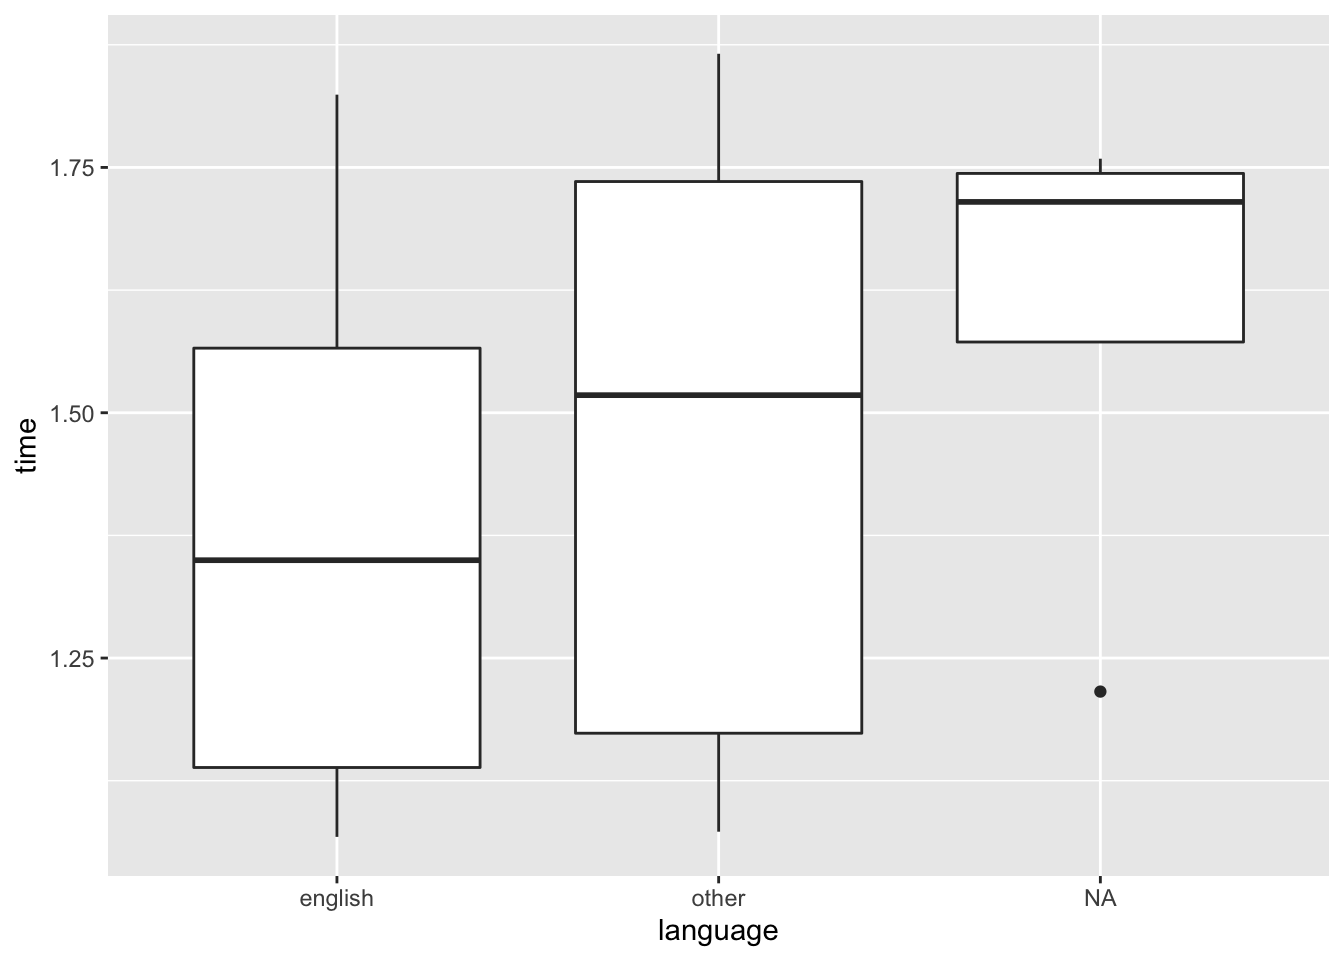
\includegraphics{r4psych_files/figure-latex/5_clean_plot-1.pdf}

There are some helper functions we haven't covered here that might help you out with \textbf{dplyr}, but you should have most of what you need now to do the majority of your data processing tasks.

\hypertarget{saving-data}{%
\section{Saving Data}\label{saving-data}}

Finally, we should look at saving our data. There are a few ways we can do this.

\hypertarget{csv-files}{%
\subsection{CSV Files}\label{csv-files}}

One way is to save your data as a .csv file, in a similar format to the data you loaded into R. However, this way we lose any customised data types (such as start and end times being POSIXct) if we are to load the data back up into R. Still, it's always good to have a copy of your data that is platform agnostic, so we should save it as a .csv so other people can load it up with any program they like. This format is also good for exploring your data in excel.

We'll save our data in the outputs folder as a csv, using the \texttt{write\_csv()} function from \textbf{readr} \citep{R-readr}, a part of the \textbf{tidyverse} \citep{R-tidyverse}.

To save the data, we just need to specify the object to save (the table of your data) in the \texttt{write\_csv()} function, along with the path to save the data. Here, we've specified that we want to save the data in the ouputs folder, and then given it a name. Folders are separated by a forwardslash, with the last string of text representing the file name. File names must end with .csv to specify the file type.

\begin{Shaded}
\begin{Highlighting}[]
\FunctionTok{write\_csv}\NormalTok{(demo\_clean, }\StringTok{"outputs/filtered\_demographic\_data.csv"}\NormalTok{)}
\end{Highlighting}
\end{Shaded}

We could also save the data as an excel file, but it's generally best to keep platform agnostic for your data backups. If you want to save your data in a useful format for further manipulation, save it as an RData file! That way, you can keep using R to work with your objects.

\hypertarget{r-data-files}{%
\subsection{R Data Files}\label{r-data-files}}

You don't want to re-run all of your pre-analysis code every time you want to make a graph/model data, so saving your data after cleaning it up is generally a good idea. However, some of the R-specific information can get lost when saving as a .csv or other format (e.g.~dates will be re-loaded as characters unless otherwise specified). Instead, we can save as an RData file which retains this information. Additionally, RData files generally take up less space on your hard drive than a .csv. Finally, we can save object types which don't play well with .csv and other formats in an RData file, such as model outputs and nested data sets (which is pretty advanced; think of a table of data within each cell of a larger table).

Here, we will save our data as an .RData file, which we can then load up again in R for further processing. To do so, we need to specify the object(s) to save (we can save several in one data file!), and we need to specify the file as above. Here, we need to be specific by using the \texttt{file} argument to define where to save our data.

\begin{Shaded}
\begin{Highlighting}[]
\FunctionTok{save}\NormalTok{(demo\_clean, }\AttributeTok{file =} \StringTok{"outputs/filtered\_demographic\_data.RData"}\NormalTok{)}
\end{Highlighting}
\end{Shaded}

When it comes to loading RData files back up, we just need to use the \texttt{load()} function from baseR. Bear in mind that the names of the objects you've saved in the data file will be the same ones you see on loading, so use informative names! Here, we just need to specify the path from which to load our data.

\begin{Shaded}
\begin{Highlighting}[]
\FunctionTok{load}\NormalTok{(}\StringTok{"outputs/filtered\_demographic\_data.RData"}\NormalTok{)}
\end{Highlighting}
\end{Shaded}

\hypertarget{exercises-4}{%
\section{Exercises}\label{exercises-4}}

We'll try some exercises to get you used to using all of the functions we've discussed here.

For these exercises we'll a simulated data set I created in the \textbf{data\_generation} folder which is saved to the inputs folder as \texttt{sim\_data.RData}. This data was saved as a tibble in the RData file, so we just use \texttt{load()} to open this data into R.

\begin{Shaded}
\begin{Highlighting}[]
\CommentTok{\# load libraries}
\FunctionTok{library}\NormalTok{(tidyverse)}
\FunctionTok{library}\NormalTok{(lubridate)}

\CommentTok{\# load data}
\FunctionTok{load}\NormalTok{(}\StringTok{"inputs/sim\_data.RData"}\NormalTok{)}
\end{Highlighting}
\end{Shaded}

This data set looks at reaction times in spotting a target when people have had caffeine or not, and when they respond with their dominant or non-dominant hand. This data set is entirely made up, so we can't be sure how realistic these results are.

First, you should take a look at your data to understand it. A simple first step is to see what the data table itself looks like.

\begin{Shaded}
\begin{Highlighting}[]
\FunctionTok{glimpse}\NormalTok{(data)}
\end{Highlighting}
\end{Shaded}

\begin{verbatim}
## Rows: 100
## Columns: 5
## $ subject  <int> 1, 2, 3, 4, 5, 6, 7, 8, 9, 10, 11, 12, 13, 14, 15, 16, 17, 18~
## $ age      <int> 34, 56, 23, 53, 44, 21, 55, 47, 29, 31, 35, 56, 34, 62, 56, 2~
## $ caffeine <fct> no, no, no, no, no, no, no, no, no, no, no, no, no, no, no, n~
## $ response <fct> non-dominant, non-dominant, non-dominant, non-dominant, non-d~
## $ DV       <dbl> 398.6627, 396.3824, 400.1234, 401.9182, 397.6403, 398.8435, 3~
\end{verbatim}

After this, we should make a more detailed plot to understand the general trends in the data.

\hypertarget{question-1-4}{%
\subsection{Question 1}\label{question-1-4}}

Make a plot of your data which looks at the relationship beween \textbf{caffeine} and \textbf{DV}. Split this plot into two to show the differences across the two response conditions.

What are the general trends in the data?

\hypertarget{question-2-4}{%
\subsection{Question 2}\label{question-2-4}}

Subset your data to remove the ages from the data set.

\hypertarget{question-3-4}{%
\subsection{Question 3}\label{question-3-4}}

Rename the \textbf{DV} column to something more informative, like \textbf{reaction\_time}

\hypertarget{question-4-4}{%
\subsection{Question 4}\label{question-4-4}}

What if we care about differences in the ages? Let's assume we have a prediction that caffeine only has an effect on those above 30 years of age. Subset your data to just those above 30 years of age.

\hypertarget{question-5-4}{%
\subsection{Question 5}\label{question-5-4}}

Rearrange the data set by age, starting from the \textbf{highest} age.

\hypertarget{question-6-4}{%
\subsection{Question 6}\label{question-6-4}}

Calculate mean centered scores for each subject and add these to a new column called \textbf{DV\_c} (DV, centered). The formula for this is \texttt{subjects\_score\ -\ mean(all\_scores)}. Can you work out what the mean should (approximately) be?

\hypertarget{question-7-4}{%
\subsection{Question 7}\label{question-7-4}}

Let's assume we have a prediction that response times should be slower above 30 years of age. Create a new column, \textbf{age\_group} that puts participants into two groups \textbf{30\_or\_under}, and \textbf{above\_30}.

\emph{Hint}: Look up the \texttt{ifelse()} function using \texttt{?ifelse()} to see how you can use logical operations to achieve this.

\hypertarget{question-8-4}{%
\subsection{Question 8}\label{question-8-4}}

Calculate the mean, standard deviation, and number of observations for each group.

\hypertarget{question-9-4}{%
\subsection{Question 9}\label{question-9-4}}

Calculate the mean, standard deviation, and number of observations for each group, excluding those with the 3 highest ages from each group.

\hypertarget{question-10-3}{%
\subsection{Question 10}\label{question-10-3}}

Take the data and do this all together:

\begin{enumerate}
\def\labelenumi{\arabic{enumi}.}
\tightlist
\item
  Rename the DV column to \textbf{response\_time}.
\item
  Remove any observations where the age of the participant is above 60.
\item
  Combine the two columns, age and caffeine, into one column called condition. Hint: Use \texttt{paste()} here. Use an underscore separator for the condition names.
\item
  Remove the caffeine and response columns and reorder the data so we have subject first, followed by age, condition, and response\_time.
\item
  Calculate mean, standard deviation, and n for condition on the response time column. Call your new column names anything sensible.
\end{enumerate}

\hypertarget{question-11-1}{%
\subsection{Question 11}\label{question-11-1}}

Was there any point in us combining the two factors into a single condition column? Do the same process above without making a summary of the data. Feed this data into a boxplot, with condition on the x-axis, and response\_time on the y-axis.

\hypertarget{simple-statistical-tests}{%
\chapter{Simple Statistical Tests}\label{simple-statistical-tests}}

In this session, we'll cover some of the most basic tests that you might use in your research. While we'll focus on selecting different tests for different scenarios, at the end of this section we'll focus on the \textbf{general linear model}, and how you can specify almost any relationship using this framework. In this session, we will cover unifactorial tests with only 2 levels in a factor. In the next session, we will cover more complicated designs.

Specifically, we'll cover:

\begin{itemize}
\tightlist
\item
  correlations
\item
  one-sample, paired, and independent \emph{t}-tests
\item
  one-way ANOVA
\item
  simple linear regression
\end{itemize}

Throughout, we will calculate descriptive statistics for our data.

This section assumes some familiarity with basic statistics. It is beyond the score of this section to teach the basics behind all of these methods, but we will cover some background on how these methods work, and why you might choose to use them in different scenarios.

\hypertarget{getting-started-3}{%
\section{Getting Started}\label{getting-started-3}}

As always, we first need to load the \texttt{tidyverse} set of packages for this Chapter.

\begin{Shaded}
\begin{Highlighting}[]
\FunctionTok{library}\NormalTok{(tidyverse)}
\end{Highlighting}
\end{Shaded}

In this session, we'll use simulated data, and data from real studies using the the \href{https://sites.trinity.edu/osl}{Open Stats Lab (OSL)} resources (hosted on my GitHub account). For each section/analysis, we'll just load the data as and when we need it.

\hypertarget{correlation}{%
\section{Correlation}\label{correlation}}

We use correlations when we want to see if there's a significant relationship between some observed variables.

More specifically, we have to know a little bit about variance, covariance, and correlation coefficients to grasp correlation and other tests.

\textbf{Variance} tells you how much your data is spread out from the mean, it's the average of the squared differences from the mean. Why do we square the differences? That's so negative values don't cancel out positive values, so we can still have an idea of how much our scores vary.

No variance (i.e.~all values are the same) is 0, and larger numbers represent more variance in your data. The square root of the variance is the standard deviation, which we can use to get exact distances of our data from the mean. Your mean +- your standard deviation multiplied by 1.96 represents 95\% of the coverage of your data.

\textbf{Covariance} is similar to the variance, but rather than telling you how much one variable varies, it tells you how much two variables vary together. If we have a positive number for the covariance, we know that our variables are related to one-another. However, covariance is sensitive to the scale you have, so if you have big numbers for each variable, your covariance will also be a big number. This magnitude doesn't tell you much about how strong the relationship is between two variables. FOr that, we need the correlation coefficient.

The \textbf{correlation coefficient} is the covariance divided by the standard deviation. This just puts the covariance on a standard scale between -1 and 1, so we now have an idea of how strongly related two variables are. A correlation of 1 shows that the two are perfectly positively correlated, so an increase in one variable is followed by an increase in the other. A correlation of 0 is no relationship, and a correlation of -1 is a perfect negative relationship, where an increase in one variable is followed by a decrease in the other.

\hypertarget{analysing-real-data}{%
\subsection{Analysing Real Data}\label{analysing-real-data}}

In this example, we'll look at a study by Dawtry, Sutton, and Sibley (2015). In this study, they were interested in why people's attitudes towards increasing wealth inequality differs within developed nations. They hypothesised that wealthy people will be less supportive of wealth distribution if their social circle is primarily made up of wealthy people. This is because they should see society as being already wealthy, and thus not requiring of wealth distribution.

Our aim here is to test the simple hypothesis that people who see society as fair and are thus satisfied with the current state of affairs will less supportive of wealth redistribution.

We'll load and clean up the data set from the Open Stats Lab. For simplicity, we'll load this data directly from a csv file stored on GitHub. (To get a link for this, you must view the raw file on GitHub online.)

First, we'll load the data using \texttt{read\_csv()}, then we'll recode the reverse-scores questions of \textbf{redist2} and \textbf{redist4} so all of the questions assessing redistribution are on the same scale.

Then we'll transmute the data, keeping only the columns we need, and calculating the mean scores for perceptions of fairness and satisfaction with distribution of wealth in society (i.e.~one factor), and mean support for redistribution (our second factor).
During this process, we'll also keep the participant IDs. Finally, we'll make everything lowercase, because it looks better!

\begin{Shaded}
\begin{Highlighting}[]
\CommentTok{\# variables}
\NormalTok{scale\_max }\OtherTok{\textless{}{-}} \DecValTok{6}

\CommentTok{\# load and clean data}
\NormalTok{corr\_data }\OtherTok{\textless{}{-}} \FunctionTok{read\_csv}\NormalTok{(}
  \StringTok{"https://raw.githubusercontent.com/gpwilliams/r4psych/master/lesson\_materials/06\_simple\_statistical\_tests/inputs/dawtry{-}et{-}al\_2015.csv"}
\NormalTok{  ) }\SpecialCharTok{\%\textgreater{}\%}
  \FunctionTok{mutate}\NormalTok{(}\AttributeTok{redist2 =}\NormalTok{ (scale\_max }\SpecialCharTok{+} \DecValTok{1}\NormalTok{) }\SpecialCharTok{{-}}\NormalTok{ redist2,}
         \AttributeTok{redist4 =}\NormalTok{ (scale\_max }\SpecialCharTok{+} \DecValTok{1}\NormalTok{) }\SpecialCharTok{{-}}\NormalTok{ redist4) }\SpecialCharTok{\%\textgreater{}\%}
  \FunctionTok{transmute}\NormalTok{(PS, }
            \AttributeTok{Fair\_Satisfied =}\NormalTok{ (fairness }\SpecialCharTok{+}\NormalTok{ satisfaction) }\SpecialCharTok{/} \DecValTok{2}\NormalTok{,}
            \AttributeTok{Support =}\NormalTok{ (redist1 }\SpecialCharTok{+}\NormalTok{ redist2 }\SpecialCharTok{+}\NormalTok{ redist3 }\SpecialCharTok{+}\NormalTok{ redist4) }\SpecialCharTok{/} \DecValTok{4}
\NormalTok{            ) }\SpecialCharTok{\%\textgreater{}\%}
  \FunctionTok{rename\_all}\NormalTok{(tolower)}
\end{Highlighting}
\end{Shaded}

\begin{verbatim}
## Rows: 305 Columns: 37
## -- Column specification ------------------------------------
## Delimiter: ","
## dbl (37): PS, PD_15, PD_30, PD_45, PD_60, PD_75, PD_90, PD_105, PD_120, PD_1...
## 
## i Use `spec()` to retrieve the full column specification for this data.
## i Specify the column types or set `show_col_types = FALSE` to quiet this message.
\end{verbatim}

\begin{Shaded}
\begin{Highlighting}[]
\NormalTok{corr\_data}
\end{Highlighting}
\end{Shaded}

\begin{verbatim}
## # A tibble: 305 x 3
##       ps fair_satisfied support
##    <dbl>          <dbl>   <dbl>
##  1   233            1      5.5 
##  2   157            3.5    3.25
##  3   275            5      3.75
##  4   111            7      2.75
##  5    52            4.5    3   
##  6    11            2.5    3.75
##  7    76            3      4.25
##  8    90            4.5    3.5 
##  9    93            4      3.75
## 10   104            4.5    3.5 
## # ... with 295 more rows
\end{verbatim}

Next, we'll calculate some means and standard deviations for these two factors of interest. We've used the \texttt{summarise\_at()} version of the \texttt{summarise()} function, as this allows us to pass two column names, and a list of functions by which to produce our statistics. We can either just pass the functions in a list, or as here give names to these functions which will be appended to the names of the variables in the table.

\begin{Shaded}
\begin{Highlighting}[]
\NormalTok{corr\_data }\SpecialCharTok{\%\textgreater{}\%} \FunctionTok{summarise\_at}\NormalTok{(}
  \FunctionTok{c}\NormalTok{(}\StringTok{"fair\_satisfied"}\NormalTok{, }\StringTok{"support"}\NormalTok{), }
  \FunctionTok{list}\NormalTok{(}\AttributeTok{mean =}\NormalTok{ mean, }\AttributeTok{sd =}\NormalTok{ sd)}
\NormalTok{)}
\end{Highlighting}
\end{Shaded}

\begin{verbatim}
## # A tibble: 1 x 4
##   fair_satisfied_mean support_mean fair_satisfied_sd support_sd
##                 <dbl>        <dbl>             <dbl>      <dbl>
## 1                3.54         3.91              2.02       1.15
\end{verbatim}

\hypertarget{checking-assumptions}{%
\subsection{Checking Assumptions}\label{checking-assumptions}}

To decide which correlation to run, we need to check some assumptions: are the factors linearly related, and do they follow a normal distribution (assumption of normality)? We'll leave exploring the first assumption for other tests, just to save time, but we'll look into testing the assumption of normality here.

We have two methods to check for normality:

\begin{enumerate}
\def\labelenumi{\arabic{enumi}.}
\tightlist
\item
  Visual inspection of the quantile-quantile plot which plotsthe correlation between our sample (observed values) and the normal distribution.
\item
  The Shapiro-Wilk test, which is a statistical test of normality. Significant results indicate that the data are \textbf{non-normal}.
\end{enumerate}

\begin{Shaded}
\begin{Highlighting}[]
\NormalTok{corr\_data }\SpecialCharTok{\%\textgreater{}\%}
  \FunctionTok{ggplot}\NormalTok{(}\FunctionTok{aes}\NormalTok{(}\AttributeTok{sample =}\NormalTok{ fair\_satisfied)) }\SpecialCharTok{+}
    \FunctionTok{geom\_qq}\NormalTok{()}
\end{Highlighting}
\end{Shaded}

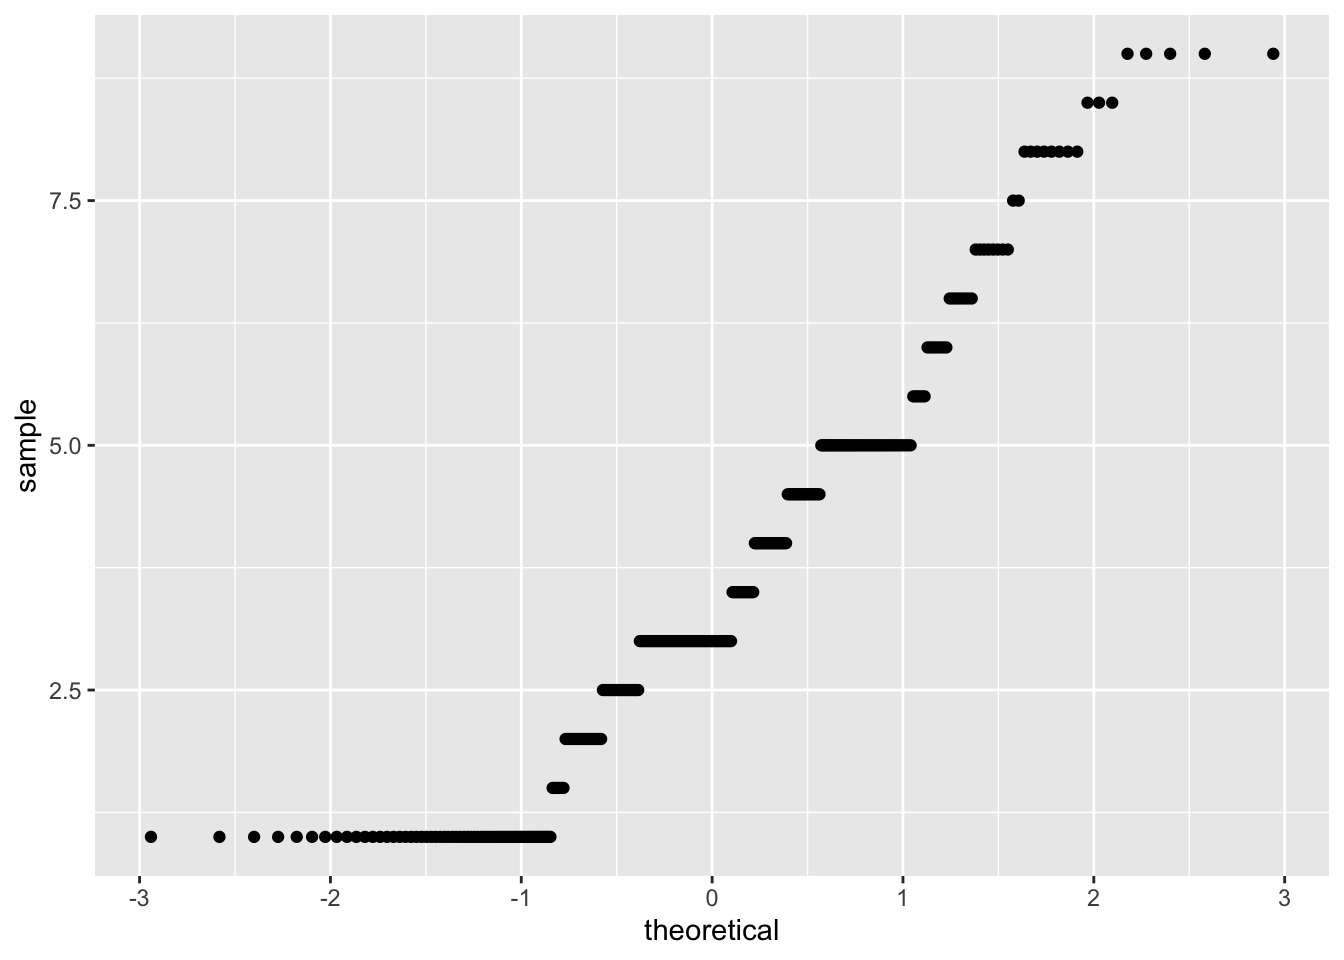
\includegraphics{r4psych_files/figure-latex/6_check_online_corr_data_assumptions_plot-1.pdf}

\begin{Shaded}
\begin{Highlighting}[]
\NormalTok{corr\_data }\SpecialCharTok{\%\textgreater{}\%}
  \FunctionTok{ggplot}\NormalTok{(}\FunctionTok{aes}\NormalTok{(}\AttributeTok{sample =}\NormalTok{ support)) }\SpecialCharTok{+}
    \FunctionTok{geom\_qq}\NormalTok{()}
\end{Highlighting}
\end{Shaded}

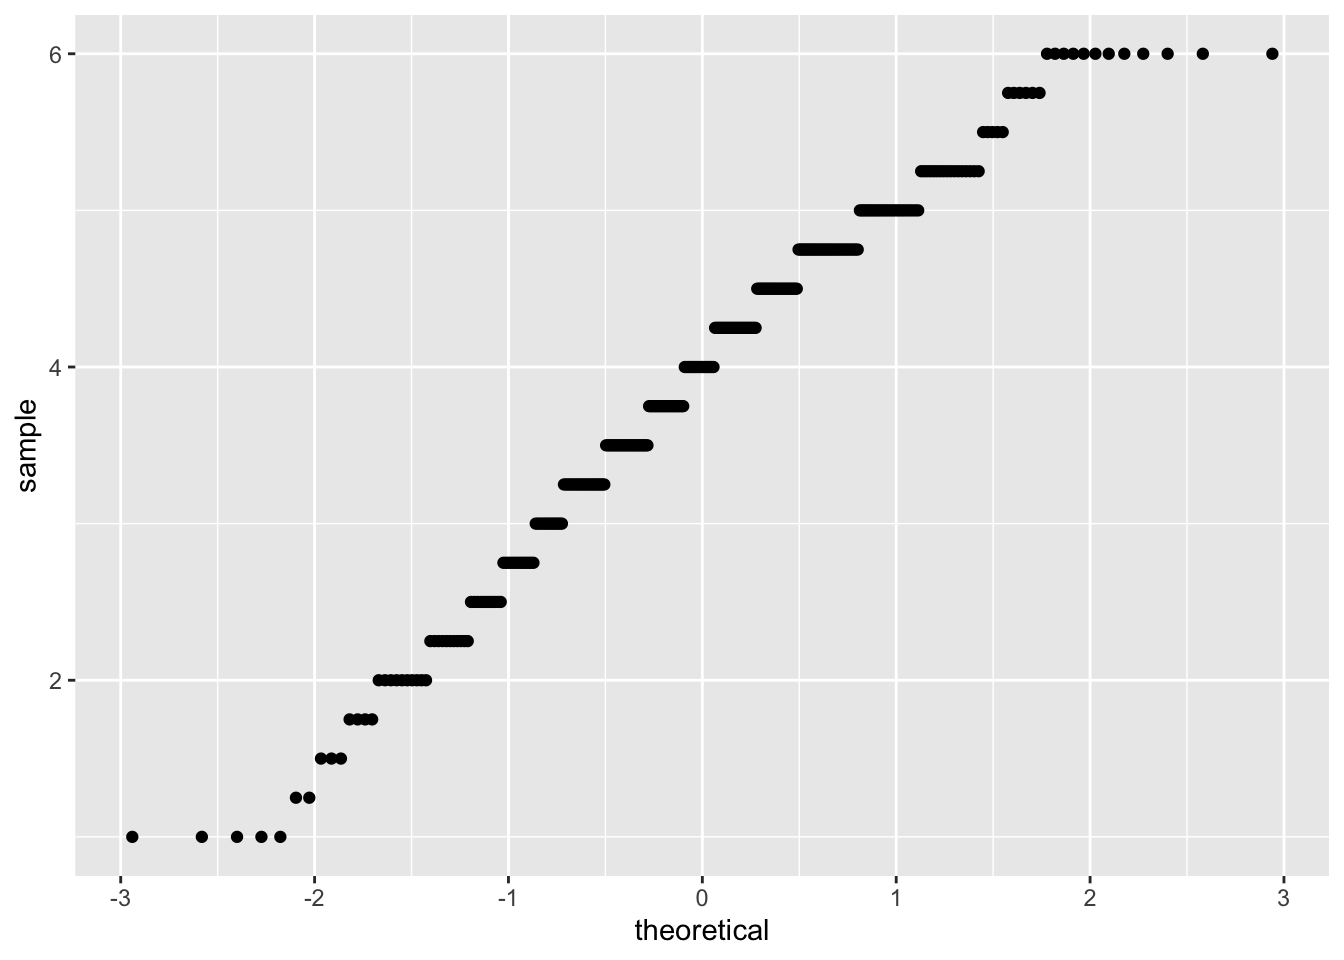
\includegraphics{r4psych_files/figure-latex/6_check_online_corr_data_assumptions_plot-2.pdf}

\begin{Shaded}
\begin{Highlighting}[]
\FunctionTok{shapiro.test}\NormalTok{(corr\_data}\SpecialCharTok{$}\NormalTok{fair\_satisfied)}
\end{Highlighting}
\end{Shaded}

\begin{verbatim}
## 
##  Shapiro-Wilk normality test
## 
## data:  corr_data$fair_satisfied
## W = 0.92602, p-value = 3.697e-11
\end{verbatim}

\begin{Shaded}
\begin{Highlighting}[]
\FunctionTok{shapiro.test}\NormalTok{(corr\_data}\SpecialCharTok{$}\NormalTok{support)}
\end{Highlighting}
\end{Shaded}

\begin{verbatim}
## 
##  Shapiro-Wilk normality test
## 
## data:  corr_data$support
## W = 0.97622, p-value = 5.993e-05
\end{verbatim}

Both the plot and test show that our data are non-normal. As such, we shouldn't use a parametric test such as Pearson's R, but we should use a non-parametric alternative. One option is Kendall's Tau, which rank orders our observations, in an attempt to account for these factors being being non-normally distributed.

\hypertarget{running-a-correlation}{%
\subsection{Running a Correlation}\label{running-a-correlation}}

Next, we'll run a correlation looking at whether there is any relationship between whether you perceive society as fair, and you're satisfied with , and your support for wealth redistribution.

Here, we'll use \texttt{cor.test()}, which takes as an argument two columns from a data.frame or matrix, which are your two factors to compare, and produces test statistics, including \emph{t}-values, \emph{p}-values, and 95\% confidence intervals.

This test defaults to use Pearson's R, and to a two-sided test of significance (i.e.~you had no predictions for the direction of effect), but you can change this to ``greater'', a positive relationship, or ``less'', a negative relationship, which will adjust \emph{p}-values accordingly.

We'll use Kendall's Tau here. Note that you simply have to replace ``kendall'' with ``pearson'' if your data do not violate any test assumptions. Also, we'll specify that we had a directional hypothesis, where there was a negative relationship between our factors (``less'').

\begin{Shaded}
\begin{Highlighting}[]
\FunctionTok{cor.test}\NormalTok{(corr\_data}\SpecialCharTok{$}\NormalTok{fair\_satisfied, corr\_data}\SpecialCharTok{$}\NormalTok{support,}
         \AttributeTok{method =} \StringTok{"kendall"}\NormalTok{,}
         \AttributeTok{alternative =} \StringTok{"less"}
\NormalTok{         )}
\end{Highlighting}
\end{Shaded}

\begin{verbatim}
## 
##  Kendall's rank correlation tau
## 
## data:  corr_data$fair_satisfied and corr_data$support
## z = -13.157, p-value < 2.2e-16
## alternative hypothesis: true tau is less than 0
## sample estimates:
##        tau 
## -0.5473132
\end{verbatim}

As you can see, we have a significant negative correlation between our two factors, indicating that as perceptions of fairness and satisfaction with society (in regards to wealth) increases, support for wealth redistribution decreases.

This is represented by the \emph{p}-value, which is below 0.05 (but see \href{https://psyarxiv.com/9s3y6}{reasons why you shouldn't mindlessly pick 0.05 as your \emph{p}-value}). Simply, the \emph{p}-value tells you how often you might observe an effect as large or larger than you one you've found in the long run (i.e.~infinite sampling) assuming the null hypothesis is true. If your \emph{p}-value is below 0.05 by convention we assume that this is an acceptable false-positve rate, as we'd only wrongly accept our results as showing an effect when there isn't one present at a rate below 5\%. Yes, Neyman-Pearson statistics is weird.

Kendall's Tau is a measure of the association between two factors. For Pearson's R (again, a measure of association), you should typically interpret the R value as \(R^2\), which shows how the percentage of variation in one variable is explained by another.

\hypertarget{t-tests}{%
\section{\texorpdfstring{\emph{t}-tests}{t-tests}}\label{t-tests}}

\emph{t}-tests allow us to see whether two means are significantly different from one another. Here, we'll get a \emph{t}-value and \emph{p}-value. The \emph{t}-value is the ratio of the difference between two groups of scores and the difference within the groups of scores. A larger \emph{t}-value tells us the difference between the groups is large, and a smaller value tells us the difference is small (i.e.~they are similar to one another). Nicely, a \emph{t}-value of 10 tells us that the groups are 10 times as different from one another as they are within each other.

For this next analysis, we'll look at the \textbf{lexdec} data set from the \texttt{languageR} library that we've used in previous sessions. We'll do this to save time on filtering the data too much, as above. The only thing we have to do is to remove the subjects we simulated for the other exercises (i.e.~22-30), so we only have real data.

Can you understand the code below? Ask yourself, why might we use \texttt{as.character(22:30)} to state which subjects we should drop?

\begin{Shaded}
\begin{Highlighting}[]
\NormalTok{lexdec }\OtherTok{\textless{}{-}} \FunctionTok{read\_csv}\NormalTok{(}\StringTok{"inputs/lexical\_decision\_raw\_data.csv"}\NormalTok{) }\SpecialCharTok{\%\textgreater{}\%}
  \FunctionTok{filter}\NormalTok{(}\SpecialCharTok{!}\NormalTok{subject }\SpecialCharTok{\%in\%}\NormalTok{ (}\FunctionTok{as.character}\NormalTok{(}\DecValTok{22}\SpecialCharTok{:}\DecValTok{30}\NormalTok{)))}
\end{Highlighting}
\end{Shaded}

\hypertarget{one-sample-t-tests}{%
\subsection{\texorpdfstring{One-Sample \emph{t}-tests}{One-Sample t-tests}}\label{one-sample-t-tests}}

Here, we want to assess whether the frequencies of words in the study (i.e.~how often people use these words) differed significantly from some baseline value of word frequency.

For this, we'll use a one-sample \emph{t}-test, which compares our scores to a known average value whether the variance of the population is not known.

We can assume that word frquency is calculated from many observations, and as such the frequency is an aggregate score, so it is appropriate to submit summaires of word frquency to a \emph{t}-test.

\hypertarget{preparing-the-data}{%
\subsubsection{Preparing the Data}\label{preparing-the-data}}

First, we have to subset our raw data, which contains information on the subjects and items tested, and only get scores for the word frequencies.

\begin{Shaded}
\begin{Highlighting}[]
\NormalTok{lexdec\_onesamp }\OtherTok{\textless{}{-}}\NormalTok{ lexdec }\SpecialCharTok{\%\textgreater{}\%} 
  \FunctionTok{group\_by}\NormalTok{(word) }\SpecialCharTok{\%\textgreater{}\%}
  \FunctionTok{summarise}\NormalTok{(}\AttributeTok{freq =} \FunctionTok{mean}\NormalTok{(frequency))}
\end{Highlighting}
\end{Shaded}

Below, we'll use the \texttt{t.test()} function to run a \emph{t}-test. Here, we input as the first value the data or scores we want to test, and in the second part, we specify the mean score in the population (mu) by which to compare the scores.

\hypertarget{running-the-test}{%
\subsubsection{Running the Test}\label{running-the-test}}

\begin{Shaded}
\begin{Highlighting}[]
\FunctionTok{t.test}\NormalTok{(lexdec\_onesamp}\SpecialCharTok{$}\NormalTok{freq, }\AttributeTok{mu =} \DecValTok{4}\NormalTok{)}
\end{Highlighting}
\end{Shaded}

\begin{verbatim}
## 
##  One Sample t-test
## 
## data:  lexdec_onesamp$freq
## t = 5.2044, df = 78, p-value = 1.535e-06
## alternative hypothesis: true mean is not equal to 4
## 95 percent confidence interval:
##  4.463784 5.038436
## sample estimates:
## mean of x 
##   4.75111
\end{verbatim}

As we can see, there is a significant difference between the frequencies for our sampled words and our assumption for the mean word frequency for all words. Again, we get \emph{t} and \emph{p} values, as well as the 95\% confidence interval for our scores.

\hypertarget{independent-samples-t-tests}{%
\subsection{\texorpdfstring{Independent-Samples \emph{t}-tests}{Independent-Samples t-tests}}\label{independent-samples-t-tests}}

Here, we'll explore a different question, which is does the native language of the speaker, English or ``other'', have any impact on reaction times to the task?

First, we have to prepare our data.

\hypertarget{preparing-the-data-1}{%
\subsubsection{Preparing the Data}\label{preparing-the-data-1}}

We need to create scores aggregated by subject, as our raw data contains information on each subject and the items they responded to. To do this, we just need to calcualte a mean score over all items for each subject in the study. We'll use the \texttt{group\_by()} and \texttt{summarise()} functions from \textbf{dplyr} to do this.

Additionally, we'll calculate log-transformed mean reaction times. This is because reaction times are typically not normally distributed, so we should transform them to make them more normal prior to analysis. The log transformation is one way to achieve this.

\begin{Shaded}
\begin{Highlighting}[]
\NormalTok{lexdec\_ind }\OtherTok{\textless{}{-}}\NormalTok{ lexdec }\SpecialCharTok{\%\textgreater{}\%} 
  \FunctionTok{group\_by}\NormalTok{(subject, native\_language) }\SpecialCharTok{\%\textgreater{}\%}
  \FunctionTok{summarise}\NormalTok{(}\AttributeTok{log\_RT =} \FunctionTok{mean}\NormalTok{(}\FunctionTok{log}\NormalTok{(RT), }\AttributeTok{na.rm =}\NormalTok{ T))}
\end{Highlighting}
\end{Shaded}

\begin{verbatim}
## `summarise()` has grouped output by 'subject'. You can
## override using the `.groups` argument.
\end{verbatim}

We'll quickly calculate some descriptives for our study to see how the two groups look.

\begin{Shaded}
\begin{Highlighting}[]
\NormalTok{lexdec\_ind }\SpecialCharTok{\%\textgreater{}\%} 
  \FunctionTok{group\_by}\NormalTok{(native\_language) }\SpecialCharTok{\%\textgreater{}\%}
  \FunctionTok{summarise}\NormalTok{(}\AttributeTok{mean\_log\_RT =} \FunctionTok{mean}\NormalTok{(log\_RT, }\AttributeTok{na.rm =}\NormalTok{ T),}
            \AttributeTok{sd\_log\_RT =} \FunctionTok{sd}\NormalTok{(log\_RT, }\AttributeTok{na.rm =}\NormalTok{ T),}
            \AttributeTok{n =} \FunctionTok{n}\NormalTok{())}
\end{Highlighting}
\end{Shaded}

\begin{verbatim}
## # A tibble: 2 x 4
##   native_language mean_log_RT sd_log_RT     n
##   <chr>                 <dbl>     <dbl> <int>
## 1 English                6.33    0.0982    11
## 2 Other                  6.47    0.178      9
\end{verbatim}

\hypertarget{running-the-test-1}{%
\subsubsection{Running the Test}\label{running-the-test-1}}

As our data are in a long format, we have to do the \emph{t}-test using a formula, seeing as our log\_RT column contains data for both conditions of the experiment. We simply specify our formula like this:

\texttt{dependent\ variable\ \textasciitilde{}\ condition}

The \texttt{\textasciitilde{}} (read: \href{https://www.youtube.com/watch?v=InPByzCDoA4}{tilde}) simply says that the thing on the left is a function of the thing on the right; i.e.~our scores are a function of our conditions.

Additionally, we specify where the data is stored (lexdec\_ind), and whether the data are paired (i.e.~paired-samples test) or not (i.e.~independent-samples test). Here, we specify \texttt{FALSE}, as we want an independent samples \emph{t}-test.

\begin{Shaded}
\begin{Highlighting}[]
\FunctionTok{t.test}\NormalTok{(log\_RT }\SpecialCharTok{\textasciitilde{}}\NormalTok{ native\_language, }\AttributeTok{data =}\NormalTok{ lexdec\_ind, }\AttributeTok{paired =} \ConstantTok{FALSE}\NormalTok{)}
\end{Highlighting}
\end{Shaded}

\begin{verbatim}
## 
##  Welch Two Sample t-test
## 
## data:  log_RT by native_language
## t = -2.2213, df = 11.903, p-value = 0.0465
## alternative hypothesis: true difference in means between group English and group Other is not equal to 0
## 95 percent confidence interval:
##  -0.29139463 -0.00268428
## sample estimates:
## mean in group English   mean in group Other 
##              6.326837              6.473876
\end{verbatim}

We can see that there is a significant difference between the two groups. Inspection of the log-transformed means shows us that reaction times are generally quicker for English speakers than non-English speakers. This is unsurprising considering the lexical decisions were made for English words.

You might notice that the degrees of freedom here are not integers (i.e.~whole numbers). That's because R defaults to using Welch's t-test, which does not make the assumption of homogeneity of variance (which is generally a good thing). Due to not making this assumption, the degrees of freedom and p-value are adjusted slightly.

\hypertarget{checking-assumptions-1}{%
\subsubsection{Checking Assumptions}\label{checking-assumptions-1}}

As with many tests \emph{t}-tests make a number of assumptions, some of which are easily handled (e.g.~are the data scalar or ordinal and randomly sampled with a large sample size?). However, these tests also assume that the data are normally distributed. We've done this for the correlation above, so we won't do it again here. However, a final assumption is homogeneity of variance, in which the variance across our samples should be roughly equal. To test for this, we can run a Barlett test for parametric data, or a Fligner test for non-parametric data (using \texttt{fligner.test()}).

Here, we'll run the Barlett test:

\begin{Shaded}
\begin{Highlighting}[]
\FunctionTok{bartlett.test}\NormalTok{(log\_RT }\SpecialCharTok{\textasciitilde{}}\NormalTok{ native\_language, }\AttributeTok{data =}\NormalTok{ lexdec\_ind)}
\end{Highlighting}
\end{Shaded}

\begin{verbatim}
## 
##  Bartlett test of homogeneity of variances
## 
## data:  log_RT by native_language
## Bartlett's K-squared = 2.9197, df = 1, p-value = 0.08751
\end{verbatim}

We got a non-significant result from this test, which indicates that the variances are not significantly different from one another, and so we've met this test assumption.

Note that we should check this before running any analyses, but I didn't want to introduce the formula notation in assumption checks.

\hypertarget{paired-samples-t-tests}{%
\subsection{\texorpdfstring{Paired-Samples \emph{t}-tests}{Paired-Samples t-tests}}\label{paired-samples-t-tests}}

Paired-samples \emph{t}-tests are run in the same way as independent-samples tests, only we need to set \texttt{paired} to \texttt{FALSE} within the \emph{t}-test call.

We'll quickly simulate some data to show how this might work. Here, we'll simulate data for a stroop task, where subjects name words (colour names; e.g.~green, blue, red) which are in different colours. Our hypothesis is that they will say the name more quickly if the word and colour are the same (congruent), and they will be slower if they mismatch (incongruent).

We'll generate 60 subjects, with the congruent reaction time being around 400ms, and the incongruent reaction time being on average 30ms slower than this.

Finally, we'll gather the data together, assuming you'll often have your data in a long format.

\begin{Shaded}
\begin{Highlighting}[]
\FunctionTok{set.seed}\NormalTok{(}\DecValTok{1000}\NormalTok{)}
\NormalTok{stroop\_dat }\OtherTok{\textless{}{-}} \FunctionTok{tibble}\NormalTok{(}
  \AttributeTok{subject =} \FunctionTok{seq}\NormalTok{(}\DecValTok{1}\SpecialCharTok{:}\DecValTok{60}\NormalTok{),}
  \AttributeTok{congruent =} \FunctionTok{rnorm}\NormalTok{(}\AttributeTok{mean =} \DecValTok{400}\NormalTok{, }\AttributeTok{sd =} \DecValTok{30}\NormalTok{, }\AttributeTok{n =} \DecValTok{60}\NormalTok{),}
  \AttributeTok{incongruent =}\NormalTok{ congruent }\SpecialCharTok{+} \FunctionTok{rnorm}\NormalTok{(}\AttributeTok{mean =} \DecValTok{30}\NormalTok{, }\AttributeTok{sd =} \DecValTok{10}\NormalTok{, }\AttributeTok{n =} \DecValTok{60}\NormalTok{)}
\NormalTok{  ) }\SpecialCharTok{\%\textgreater{}\%}
  \FunctionTok{gather}\NormalTok{(}\AttributeTok{key =}\NormalTok{ condition, }\AttributeTok{value =}\NormalTok{ reaction\_time, }\DecValTok{2}\SpecialCharTok{:}\DecValTok{3}\NormalTok{) }\SpecialCharTok{\%\textgreater{}\%} 
  \FunctionTok{mutate}\NormalTok{(}
    \AttributeTok{log\_RT =} \FunctionTok{log}\NormalTok{(reaction\_time)}
\NormalTok{  )}
\end{Highlighting}
\end{Shaded}

Note that if your data is in a wide format, you specify the model formula like so:

\begin{Shaded}
\begin{Highlighting}[]
\FunctionTok{t.test}\NormalTok{(data}\SpecialCharTok{$}\NormalTok{dependent\_variable\_one, data}\SpecialCharTok{$}\NormalTok{dependent\_variable\_two, }\AttributeTok{data =}\NormalTok{ data\_name, }\AttributeTok{paired =} \ConstantTok{TRUE}\NormalTok{)}
\end{Highlighting}
\end{Shaded}

In this format, you simply give the column names for where your data is stored for each condition, and R will compare the first entry against the second. However, I typically keep my data in long format, so we will mainly use the formula format for specifying our models. Using the formula notation is also useful for more complex designs where wide formatted data is unrealistic, so we'll stick to this as our default way to specify our models.

\hypertarget{running-the-test-2}{%
\subsubsection{Running the Test}\label{running-the-test-2}}

The paired-samples \emph{t}-test formula takes the same form as the independent sampels \emph{t}-test, only with \texttt{paired\ =\ TRUE}.

\begin{Shaded}
\begin{Highlighting}[]
\FunctionTok{t.test}\NormalTok{(log\_RT }\SpecialCharTok{\textasciitilde{}}\NormalTok{ condition, }\AttributeTok{data =}\NormalTok{ stroop\_dat, }\AttributeTok{paired =} \ConstantTok{TRUE}\NormalTok{)}
\end{Highlighting}
\end{Shaded}

\begin{verbatim}
## 
##  Paired t-test
## 
## data:  log_RT by condition
## t = -25.573, df = 59, p-value < 2.2e-16
## alternative hypothesis: true mean difference is not equal to 0
## 95 percent confidence interval:
##  -0.08379794 -0.07163601
## sample estimates:
## mean difference 
##     -0.07771698
\end{verbatim}

As with the independent-samples t-test, we get all of the same statistics in the output.

Here, there is a significant difference between the two conditions, with participants responding to items more quickly in the congruent when compared to the incongruent condition. This makes sense, as the name and ink colour both match, so there's no interference during processing.

\hypertarget{anova}{%
\section{ANOVA}\label{anova}}

Like the \emph{t}-value, the F value from an ANOVA lets you know whether two groups of scores are similar or different from one another. More specifically, it gives you the ratio of the variance between two samples.

As ANOVAs and \emph{t}-tests are both part of the general linear model family, the outputs of both tests are similar when we have only 2 levels of a condition. Compare the results of the following analyses with those from the \emph{t}-tests aboves.

We use the \texttt{aov()} function in R to perform an analysis of variance. With the ANOVA and linear models we will explore later, we get a lot of information from the output just by running the \texttt{aov()} function. As such, we'll assign this to an object, which can just be a name in which to store our output of the model. After this, we use the \texttt{summary()} function, to get a neat summary of the statistics that we want to look at.

\hypertarget{one-way-anova}{%
\subsection{One-Way ANOVA}\label{one-way-anova}}

\hypertarget{indpendent-samples-anova}{%
\subsubsection{Indpendent-Samples ANOVA}\label{indpendent-samples-anova}}

We'll simply refit the same data from the \texttt{lexdec} data set to get an idea of how similar \emph{t}-tests and ANOVAs are. Again, we just need to specify our DV to the left of the condition.

\begin{Shaded}
\begin{Highlighting}[]
\NormalTok{anova\_ind }\OtherTok{\textless{}{-}} \FunctionTok{aov}\NormalTok{(log\_RT }\SpecialCharTok{\textasciitilde{}}\NormalTok{ native\_language, }\AttributeTok{data =}\NormalTok{ lexdec\_ind)}
\FunctionTok{summary}\NormalTok{(anova\_ind)}
\end{Highlighting}
\end{Shaded}

\begin{verbatim}
##                 Df Sum Sq Mean Sq F value Pr(>F)  
## native_language  1 0.1070 0.10702   5.523 0.0304 *
## Residuals       18 0.3488 0.01938                 
## ---
## Signif. codes:  0 '***' 0.001 '**' 0.01 '*' 0.05 '.' 0.1 ' ' 1
\end{verbatim}

As before, we have a significant difference between the two language groups on their log reaction times in the lexical decision task.

\hypertarget{paired-samples-anova}{%
\subsubsection{Paired-Samples ANOVA}\label{paired-samples-anova}}

For a paired-sampels ANOVA, we just need to specify our models as before, but we also need to include an error term. This error term takes the form of:

\texttt{Error(observation\_unit/factor)}

We always need to specify that this is an error term we're adding, hence the name \texttt{Error()}. We then need to specify what our error term is. Since we're using a paired-samples test, where the same people ttake part in both conditions, we need to tell R that our error term is for the condition factor within subjects, i.e.~different people might react differently to the conditions. Finally, as always we need to specify where our data lies.

Below, we'll just refit the stroop data from the \emph{t}-test example above.

\begin{Shaded}
\begin{Highlighting}[]
\NormalTok{anova\_paired }\OtherTok{\textless{}{-}} \FunctionTok{aov}\NormalTok{(log\_RT }\SpecialCharTok{\textasciitilde{}}\NormalTok{ condition }\SpecialCharTok{+} \FunctionTok{Error}\NormalTok{(subject}\SpecialCharTok{/}\NormalTok{condition), }\AttributeTok{data =}\NormalTok{ stroop\_dat)}
\FunctionTok{summary}\NormalTok{(anova\_paired)}
\end{Highlighting}
\end{Shaded}

\begin{verbatim}
## 
## Error: subject
##           Df   Sum Sq  Mean Sq F value Pr(>F)
## Residuals  1 0.005198 0.005198               
## 
## Error: subject:condition
##           Df Sum Sq Mean Sq
## condition  1 0.1359  0.1359
## 
## Error: Within
##            Df Sum Sq Mean Sq F value  Pr(>F)   
## condition   1 0.0453 0.04535   8.302 0.00472 **
## Residuals 116 0.6336 0.00546                   
## ---
## Signif. codes:  0 '***' 0.001 '**' 0.01 '*' 0.05 '.' 0.1 ' ' 1
\end{verbatim}

As before, we have a significant difference between the two congruency conditions on their log reaction times in the lexical decision task.

\hypertarget{linear-regression}{%
\section{Linear Regression}\label{linear-regression}}

In this section, we'll look at linear regression. We would typically fit a linear model when we predict a linear relationship between one or more variable(s), e.g.~\(X\), and a continuous dependent variable, e.g.~\(Y\). This relationship for any one subject (or item) can be described as:

\[Y = \beta_0 + \beta_1 X + e\]
Where \(Y\), the outcome or dependent variable, is calcualted by the individual's intercept value \(\beta_0\) (i.e.~typically the score at 0 on the x-axis of a graph), their slope term \(\beta_1\), or how much to increase their \(Y\) value for every tick of the x-axis, multiplied by their value along the X axis (\(X\)), and an error term \(e\), which is the residual error from our model.

The residual error (or simply residuals) show the difference between our predicted values from our model and observed values from our data. (Remember our QQ-plot? This looks at how your residuals are distributed. If they are normally distributed, then we're OK!)

We have this error term as we do not want to fit a perfect model to our data. If we did that, our model would work very well for our exact sample, but it wouldn't work so well for more generalised cases (e.g.~with other samples). As such, we do not \textbf{overfit} our model so that it keeps some explanatory power for broader cases.

Like \emph{t}-tests and ANOVAs, linear regression is simply another way for us to analyse our data. The general linear model is very useful in that it can be applied to the simplest and most complex cases of analyses, and really, it's likely this is all you'll need to know. Nicely, our predictors can be scalar data (e.g.~quantifying the success of different doses of a drug) or categorical (e.g.~different conditions; drug or no drug).

\hypertarget{general-linear-model}{%
\subsection{General Linear Model}\label{general-linear-model}}

We use the general linear model when we have outcome data that is a continuous variable. However, this procedure is not appropriate when we have bounded data (e.g.~Likert scales, binomial (0 or 1) responses). In these cases, we have to use a more specific form of the model, called the \textbf{generalised linear model}, which we'll look at after this section.

\hypertarget{independent-samples-linear-model}{%
\subsubsection{Independent-Samples Linear Model}\label{independent-samples-linear-model}}

As with the \emph{t}-test and ANOVA, we'll use the \texttt{lexdec\_ind} simulated data set from before.

\hypertarget{running-the-test-3}{%
\paragraph{Running the Test}\label{running-the-test-3}}

As with the ANOVA, we need to specify our model using the formula, with our dependent variable to the left of the \texttt{\textasciitilde{}}, and our conditions to the right. Here, we'll assign this to the object \texttt{lm\_ind}, and we'll get a summary of the data using the \texttt{summary()} function.

\begin{Shaded}
\begin{Highlighting}[]
\NormalTok{lm\_ind }\OtherTok{\textless{}{-}} \FunctionTok{lm}\NormalTok{(log\_RT }\SpecialCharTok{\textasciitilde{}}\NormalTok{ native\_language, }\AttributeTok{data =}\NormalTok{ lexdec\_ind)}
\FunctionTok{summary}\NormalTok{(lm\_ind)}
\end{Highlighting}
\end{Shaded}

\begin{verbatim}
## 
## Call:
## lm(formula = log_RT ~ native_language, data = lexdec_ind)
## 
## Residuals:
##      Min       1Q   Median       3Q      Max 
## -0.22075 -0.07276 -0.00893  0.07599  0.33469 
## 
## Coefficients:
##                      Estimate Std. Error t value Pr(>|t|)    
## (Intercept)           6.32684    0.04197  150.75   <2e-16 ***
## native_languageOther  0.14704    0.06256    2.35   0.0304 *  
## ---
## Signif. codes:  0 '***' 0.001 '**' 0.01 '*' 0.05 '.' 0.1 ' ' 1
## 
## Residual standard error: 0.1392 on 18 degrees of freedom
## Multiple R-squared:  0.2348, Adjusted R-squared:  0.1923 
## F-statistic: 5.523 on 1 and 18 DF,  p-value: 0.03037
\end{verbatim}

Nicely, we get a lot of information from this model. As with the ANOVA, we have a test statistic (this time a \emph{t}-value) and a \emph{p}-value, under the heading \texttt{Pr(\textgreater{}\textbar{}t\textbar{})}.

The \emph{t}-value is the intercept term for our condition, divided by the standard error. The \emph{p}-value here is the proportion of the \emph{t} distribution which is greater than the \emph{t} statistic. The \emph{p}-value is just the proportion of the t distribution which is greater than the value of the t statistic (hence the weird notation).

We also get some information that is more informative than the ANOVA. We get our intercept term (\texttt{(Intercept)}), which here is mean score for the English language group. Let's see how that matches our mean scores:

\begin{Shaded}
\begin{Highlighting}[]
\NormalTok{lexdec\_means }\OtherTok{\textless{}{-}}\NormalTok{ lexdec\_ind }\SpecialCharTok{\%\textgreater{}\%} 
  \FunctionTok{group\_by}\NormalTok{(native\_language) }\SpecialCharTok{\%\textgreater{}\%} 
  \FunctionTok{summarise}\NormalTok{(}\AttributeTok{mean =} \FunctionTok{mean}\NormalTok{(log\_RT))}
\NormalTok{lexdec\_means}
\end{Highlighting}
\end{Shaded}

\begin{verbatim}
## # A tibble: 2 x 2
##   native_language  mean
##   <chr>           <dbl>
## 1 English          6.33
## 2 Other            6.47
\end{verbatim}

Under this, we have the difference from this intercept for the Other language group (\texttt{native\_languageOther}). How does this relate to the means? Below, we'll subtract the congruent scores from the incongruent scores.

\begin{Shaded}
\begin{Highlighting}[]
\NormalTok{lexdec\_means}\SpecialCharTok{$}\NormalTok{mean[}\DecValTok{2}\NormalTok{] }\SpecialCharTok{{-}}\NormalTok{ lexdec\_means}\SpecialCharTok{$}\NormalTok{mean[}\DecValTok{1}\NormalTok{]}
\end{Highlighting}
\end{Shaded}

\begin{verbatim}
## [1] 0.1470395
\end{verbatim}

As you can see, this value relates to the score for \texttt{native\_languageOther}, which shows how the Other language group differs from the baseline, English language group.

You might ask now, how did R know which condition to set as the intercept? R defaults to going alphabetically, so English comes before Other, hence it is the baseline. In simple cases like this, where we have only 2 levels, this is not a concern. But when we have more levels or factors, we need to pay attention to how we specify our contrasts in R.

Finally, in the output we have our residuals, including the residual standard error.

\hypertarget{paired-samples-linear-model}{%
\subsubsection{Paired-Samples Linear Model}\label{paired-samples-linear-model}}

As with the \emph{t}-test and ANOVA, we'll use the \texttt{stroop\_dat} simulated data set from before.

\hypertarget{running-the-test-4}{%
\paragraph{Running the Test}\label{running-the-test-4}}

As with the ANOVA, we need to specify our model using the formula, with our dependent variable to the left of the \texttt{\textasciitilde{}}, and our conditions to the right. Here, we'll assign this to the object \texttt{lm\_ind\textquotesingle{},\ and\ we\textquotesingle{}ll\ get\ a\ summary\ of\ the\ data\ using\ the}summary()` function. Unlike with \emph{t}-tests and ANOVA, we do not need to specify an error term if our data are within-subjects (or paired-samples), so we simply use the same formula for independent- and paried-samples tests. Note that this means that our model doesn't account for how much of our outcome variable is predicted by subject-specific factors (i.e.~variation between people). Some might respond more or less strongly to the effect of condition than others. As such, we can do a bit better with these models by fitting a mixed-effects model that can account for subject level effects. For now, we'll leave that for another lesson. If you want to get linear model output while accounting for by-subjects effects like in an ANOVA, head over to the next lesson!

\begin{Shaded}
\begin{Highlighting}[]
\NormalTok{lm\_pair }\OtherTok{\textless{}{-}} \FunctionTok{lm}\NormalTok{(log\_RT }\SpecialCharTok{\textasciitilde{}}\NormalTok{ condition, }\AttributeTok{data =}\NormalTok{ stroop\_dat)}
\FunctionTok{summary}\NormalTok{(lm\_pair)}
\end{Highlighting}
\end{Shaded}

\begin{verbatim}
## 
## Call:
## lm(formula = log_RT ~ condition, data = stroop_dat)
## 
## Residuals:
##       Min        1Q    Median        3Q       Max 
## -0.153786 -0.049960  0.006172  0.039194  0.202953 
## 
## Coefficients:
##                      Estimate Std. Error t value Pr(>|t|)    
## (Intercept)          5.978613   0.009499 629.391  < 2e-16 ***
## conditionincongruent 0.077717   0.013434   5.785 6.07e-08 ***
## ---
## Signif. codes:  0 '***' 0.001 '**' 0.01 '*' 0.05 '.' 0.1 ' ' 1
## 
## Residual standard error: 0.07358 on 118 degrees of freedom
## Multiple R-squared:  0.221,  Adjusted R-squared:  0.2144 
## F-statistic: 33.47 on 1 and 118 DF,  p-value: 6.066e-08
\end{verbatim}

As before, we get our intercept term (\texttt{(Intercept)}), which here is mean score for the congruent condition. Let's see how that matches our mean scores:

\begin{Shaded}
\begin{Highlighting}[]
\NormalTok{stroop\_means }\OtherTok{\textless{}{-}}\NormalTok{ stroop\_dat }\SpecialCharTok{\%\textgreater{}\%} 
  \FunctionTok{group\_by}\NormalTok{(condition) }\SpecialCharTok{\%\textgreater{}\%} 
  \FunctionTok{summarise}\NormalTok{(}\AttributeTok{mean =} \FunctionTok{mean}\NormalTok{(log\_RT))}
\NormalTok{stroop\_means}
\end{Highlighting}
\end{Shaded}

\begin{verbatim}
## # A tibble: 2 x 2
##   condition    mean
##   <chr>       <dbl>
## 1 congruent    5.98
## 2 incongruent  6.06
\end{verbatim}

Under this, we have the difference from this intercept for the congruent condition (\texttt{conditionincongruent}). How does this relate to the means? Below, we'll subtract the congruent scores from the incongruent scores.

\begin{Shaded}
\begin{Highlighting}[]
\NormalTok{stroop\_means}\SpecialCharTok{$}\NormalTok{mean[}\DecValTok{2}\NormalTok{] }\SpecialCharTok{{-}}\NormalTok{ stroop\_means}\SpecialCharTok{$}\NormalTok{mean[}\DecValTok{1}\NormalTok{]}
\end{Highlighting}
\end{Shaded}

\begin{verbatim}
## [1] 0.07771698
\end{verbatim}

As you can see, this value relates to the score for \texttt{conditionincongruent}, which shows how the incongruent condition differs from the baseline, congruent condition.

Aside from this, we have a whole host of other information that we might want to consider, including an adjusted \(R^2\), which tells us about how much our explanatory predictors (e.g.~condition) accounts for changes in the dependent variable. For now, this is all we need.

\hypertarget{assumptions}{%
\subsubsection{Assumptions}\label{assumptions}}

Simple general linear models make a few assumptions, of which:

\begin{itemize}
\tightlist
\item
  Linear relationship: your variables must be linearly related, otherwise a linear fit doesn't make sense
\item
  Normality: Variables must be normally distributed
\item
  Homoscedasticity (homogeneity of variance): your residuals are equal across the regression line
\item
  No auto-correlation: your observations for your dependent variable must not impact one-another (e.g.~eye-movements; if you get one success (i.e.~a look at an object), the next eye-movement is likely also be a success (i.e.~still looking) -- this is bad!)
\end{itemize}

We've already looked at checking for normality and homoscedasticity, so we won't do this again here. We can also decide about auto-correlation prior to running our analyses, so if you understand your data we may not need to check this assumption. But we should probably check for a linear relationship. The best way to do this is to just eye-ball the data with a plot. This makes sense if your predictor is on a scale, but it's not really defined when we have groups, so we'll leave that for now.

\hypertarget{generalised-linear-model}{%
\subsection{Generalised Linear Model}\label{generalised-linear-model}}

What about cases in which we have a binomial response, e.g.~if people got an answer correct or not? Here, we have to use a generalised linear model. This takes the same form as the general linear model, only these models use a link function, which allows the dependent variable to be a function of some error term other than the normal distribution.

We won't go into detail as to how the generalized linear model works, but just note that you can specify different link functions to describe your data, so for example if your data take a log distribution, you can specify a logit link.

We'll focus on a common case of fitting a logistic model to our data using a binomial distribution.

\hypertarget{preparing-the-data-2}{%
\subsubsection{Preparing the Data}\label{preparing-the-data-2}}

Below, we'll simulate some data looking at the effectiveness of a smoking intervention on smoking cessation rates. We have a simple outcome, 0 if people still smoke after the experiment (i.e.~a failure), and 1 if they quit smoking (i.e.~a success).

\begin{Shaded}
\begin{Highlighting}[]
\FunctionTok{set.seed}\NormalTok{(}\DecValTok{1000}\NormalTok{)}
\NormalTok{prob }\OtherTok{\textless{}{-}} \FunctionTok{rep}\NormalTok{(}\FunctionTok{c}\NormalTok{(}\FloatTok{0.3}\NormalTok{, }\FloatTok{0.6}\NormalTok{), }\DecValTok{50}\NormalTok{)}
\NormalTok{cond }\OtherTok{\textless{}{-}} \FunctionTok{rep}\NormalTok{(}\FunctionTok{c}\NormalTok{(}\StringTok{"control"}\NormalTok{, }\StringTok{"intervention"}\NormalTok{), }\DecValTok{50}\NormalTok{)}
\NormalTok{subject }\OtherTok{\textless{}{-}} \FunctionTok{seq}\NormalTok{(}\DecValTok{1}\SpecialCharTok{:}\DecValTok{100}\NormalTok{)}

\NormalTok{smoking\_dat }\OtherTok{\textless{}{-}} \FunctionTok{tibble}\NormalTok{(}
  \AttributeTok{subject =}\NormalTok{ subject,}
  \AttributeTok{cond =}\NormalTok{ cond,}
  \AttributeTok{outcome =} \FunctionTok{rbinom}\NormalTok{(}\AttributeTok{n =} \DecValTok{100}\NormalTok{, }\AttributeTok{size =} \DecValTok{1}\NormalTok{, }\AttributeTok{prob =}\NormalTok{ prob)}
\NormalTok{)}
\end{Highlighting}
\end{Shaded}

Let's see what the rates of smoking look like:

\begin{Shaded}
\begin{Highlighting}[]
\NormalTok{smoking\_dat }\SpecialCharTok{\%\textgreater{}\%} \FunctionTok{group\_by}\NormalTok{(cond) }\SpecialCharTok{\%\textgreater{}\%} \FunctionTok{summarise}\NormalTok{(}\AttributeTok{mean =} \FunctionTok{mean}\NormalTok{(outcome))}
\end{Highlighting}
\end{Shaded}

\begin{verbatim}
## # A tibble: 2 x 2
##   cond          mean
##   <chr>        <dbl>
## 1 control       0.24
## 2 intervention  0.54
\end{verbatim}

Great! It looks like our intervention worked well. If only it was that easy in real life\ldots{}

\hypertarget{running-the-test-5}{%
\subsubsection{Running the Test}\label{running-the-test-5}}

The generalised linear model is specified using the \texttt{glm()} function. Here, we can specify a few extra details about our model or accept the defaults. We'll overspecify to show these things work. Here, we've asked to fit the model using a binomial link function, using the \texttt{family\ =\ "binomial"} argument since our data come from a binomial decision and follow a binomial distribution.

\begin{Shaded}
\begin{Highlighting}[]
\NormalTok{glm\_ind }\OtherTok{\textless{}{-}} \FunctionTok{glm}\NormalTok{(outcome }\SpecialCharTok{\textasciitilde{}}\NormalTok{ cond, }\AttributeTok{data =}\NormalTok{ smoking\_dat, }\AttributeTok{family =} \StringTok{"binomial"}\NormalTok{)}
\FunctionTok{summary}\NormalTok{(glm\_ind)}
\end{Highlighting}
\end{Shaded}

\begin{verbatim}
## 
## Call:
## glm(formula = outcome ~ cond, family = "binomial", data = smoking_dat)
## 
## Deviance Residuals: 
##     Min       1Q   Median       3Q      Max  
## -1.2462  -0.7409  -0.7409   1.1101   1.6894  
## 
## Coefficients:
##                  Estimate Std. Error z value Pr(>|z|)    
## (Intercept)       -1.1527     0.3311  -3.481   0.0005 ***
## condintervention   1.3130     0.4361   3.011   0.0026 ** 
## ---
## Signif. codes:  0 '***' 0.001 '**' 0.01 '*' 0.05 '.' 0.1 ' ' 1
## 
## (Dispersion parameter for binomial family taken to be 1)
## 
##     Null deviance: 133.75  on 99  degrees of freedom
## Residual deviance: 124.10  on 98  degrees of freedom
## AIC: 128.1
## 
## Number of Fisher Scoring iterations: 4
\end{verbatim}

Again, we get a similar output to the linear model, but we've fit the data using a more appropriate model to account for the binary nature of the data. Notice that now we have z-values instead of \emph{t}-values. Aside from that, all of your other interpretations remain the same.

\hypertarget{proportion-data}{%
\subsubsection{Proportion Data}\label{proportion-data}}

We can also fit models with proportion data for the dependent variable using the \texttt{glm()} function. To do so, you need the number of successes and the number of observations, specifying your model like so:

\texttt{glm(successes/observations\ \textasciitilde{}\ cond,\ data\ =\ smoking\_dat,\ family\ =\ "binomial")}

Or, if you just have the proportion and number of observations, you can fit it like so:

\texttt{glm(proportion\ \textasciitilde{}\ cond,\ data\ =\ smoking\_dat,\ family\ =\ "binomial",\ weights\ =\ observations)}

In this last case, you just specify to weight successes by the number of observations that you had for each data point. This weighting is important when you do more advanced analyses, like growth curve analysis with transformations on your data (e.g.~empirical logit) as you can tell your model how much to ``trust'' each data point. But for our cases so far, this is all we need to know about the weights argument.

\hypertarget{exercises-5}{%
\section{Exercises}\label{exercises-5}}

If you don't have access to these, please \href{https://github.com/gpwilliams/r4psych}{download the repository from GitHub} and open the \textbf{lesson\_materials} folder. Open the relevant folder for this lesson. If you work out of the file \textbf{06\_simple\_statistical\_tests.Rmd} the code below will work to load the data set. If this fails then quit R and open it up from the .Rmd file above so your working directory is in the correct folder.

This data was saved as a .csv, so we need to use \texttt{read\_csv()} to load the data into R.

\begin{Shaded}
\begin{Highlighting}[]
\FunctionTok{library}\NormalTok{(tidyverse)}
\end{Highlighting}
\end{Shaded}

Next, we'll load all of the data sets.

\begin{Shaded}
\begin{Highlighting}[]
\NormalTok{binom\_b\_data }\OtherTok{\textless{}{-}} \FunctionTok{read\_csv}\NormalTok{(}\StringTok{"inputs/binom\_between\_data.csv"}\NormalTok{)}
\NormalTok{binom\_w\_data }\OtherTok{\textless{}{-}} \FunctionTok{read\_csv}\NormalTok{(}\StringTok{"inputs/binom\_within\_data.csv"}\NormalTok{)}
\NormalTok{bsubj\_data }\OtherTok{\textless{}{-}} \FunctionTok{read\_csv}\NormalTok{(}\StringTok{"inputs/bsubj\_data.csv"}\NormalTok{)}
\NormalTok{wsubj\_data }\OtherTok{\textless{}{-}} \FunctionTok{read\_csv}\NormalTok{(}\StringTok{"inputs/wsubj\_data.csv"}\NormalTok{)}
\NormalTok{corr\_data }\OtherTok{\textless{}{-}} \FunctionTok{read\_csv}\NormalTok{(}\StringTok{"inputs/corr\_data.csv"}\NormalTok{)}
\end{Highlighting}
\end{Shaded}

\hypertarget{question-1-5}{%
\subsection{Question 1}\label{question-1-5}}

Using the \texttt{corr\_data} data set, prepare to run a correlation for the height and weights of the participants. First, you have to check all of the assumptions are met for a parametric test. Do a visual inspection of the normality of the variables, and check that the two are linearly related.

\hypertarget{question-2-5}{%
\subsection{Question 2}\label{question-2-5}}

Using the information from Question 1, run a correlation for the height and weights of the participants. Adjust to a non-parametric test if necessary.

What is the correlation between the two variables? Can you work out the \(R^2\)? What does this tell us?

\hypertarget{question-3-5}{%
\subsection{Question 3}\label{question-3-5}}

Aggregate the scores of the \texttt{bsubj\_data} data set by subject as an object called \texttt{bsubj\_agg}. Output the mean scores aggregated by subject.

Then run a \emph{t}-test between the two groups of A. Is there a significant difference between the two conditions?

\hypertarget{question-4-5}{%
\subsection{Question 4}\label{question-4-5}}

Check that a \emph{t}-test was appropriate for question 3. We'll only check for \textbf{homogeneity of variance} here. What did the test show? Was a \emph{t}-test appropriate?

\hypertarget{question-5-5}{%
\subsection{Question 5}\label{question-5-5}}

Aggregate the \texttt{wsubj\_data} by subjects and save this as the object \texttt{wsubj\_agg}. Then submit this aggregated data to an ANOVA, saving the output as the object \texttt{wsubj\_aov}. What does the ANOVA show us?

\hypertarget{question-6-5}{%
\subsection{Question 6}\label{question-6-5}}

We should probably allow people to interpret our inferential tests with plots and descriptive statistics.

First, make a plot of the two conditions from Question 5, using your \texttt{wsubj\_agg} data set. Then, output a table of means, standard deviations, and standard errors for the two groups. To calculate the standard error you need to take the standard deviation of the dependent variable divided by the square root of number of observations for the dependent variable (i.e.~\texttt{sd(output)/sqrt(length(output))}).

\hypertarget{question-7-5}{%
\subsection{Question 7}\label{question-7-5}}

Fit a linear model to the \texttt{wsubj\_agg} data and save this as \texttt{wsubj\_lm}. How does this compare to the ANOVA from question 5? Compare the results of the parameter estimates from the linear model to that of your plot. How do these parameters compare?

\hypertarget{question-8-5}{%
\subsection{Question 8}\label{question-8-5}}

Fit a linear model to the Using the \texttt{binom\_b\_data}, and save this output as \texttt{binom\_b\_lm}. Look at the summary of the output. Is there a significant difference between the two groups?

\hypertarget{question-9-5}{%
\subsection{Question 9}\label{question-9-5}}

Fit a linear model to the Using the \texttt{binom\_w\_data}, and save this output as \texttt{binom\_b\_lm}. Look at the summary of the output. Is there a significant difference between the two groups? You will first have to convert the data to long format in order to use the formula syntax for your model. For this, set the key to ``test\_time'', and the value to ``success''.

\hypertarget{question-10-4}{%
\subsection{Question 10}\label{question-10-4}}

Using the long-formatted \texttt{binom\_w\_data} from question 9, create a table containing the calculate means, standard deviations, standard errors, and 95\% confidence intervals for the two test times.

In order to calcualte the upper and lower bounds of the 95\% confidence interval, you will have to take the mean of the dependent variable - 1.96 times the \textbf{standard error} of the mean, and the mean of the dependent variable + 1.96 times the standard error of the mean respectively. Call these columns \texttt{lower\_confint} and \texttt{upper\_confint} respectively.

Next, plot a bar plot of this data with standard error bars.

Compare your hand-coded standard errors with those from ggplot. How do they compare? Do the bounds seem similar?

\hypertarget{advanced-statistical-tests}{%
\chapter{Advanced Statistical Tests}\label{advanced-statistical-tests}}

In this session, we'll cover more advanced statistical tests, such as multifactorial experiments and experiments with factors of more than 2 levels.

Specifically, we'll cover:

\begin{itemize}
\tightlist
\item
  multilevel and multifactorial ANOVA
\item
  multilevel and multiple regression
\item
  factor coding (and why it matters in R)
\item
  sum of squares (and why this matters in R)
\end{itemize}

As with the previous section, this section assumes some familiarity with basic statistics. It is beyond the score of this section to teach the basics behind all of these methods, but we will cover some background on how these methods work, and why you might choose to use them in different scenarios.

\hypertarget{getting-started-4}{%
\section{Getting Started}\label{getting-started-4}}

As always, we first need to load the \texttt{tidyverse} set of packages for this Chapter.

\begin{Shaded}
\begin{Highlighting}[]
\FunctionTok{library}\NormalTok{(tidyverse)}
\end{Highlighting}
\end{Shaded}

\hypertarget{multilevel-analyses}{%
\section{Multilevel Analyses}\label{multilevel-analyses}}

Often, your experiments will have more than one level for a factor. However, how you code these factors determines the answers that you get from your analyses.

Take for example evaluating the efficacy of a host of drugs. We often want to compare performance of several drugs against a placebo. In this case, we might perform an analysis where we compare different levels of one factor (drug; with placebo, drug one, and drug two levels) against a reference level (drug level one; placebo). In this case, we would use \textbf{treatment} coding for our factors, as we only want to know if drug one and drug two perform differently from the placebo. That is, we are interested in the \textbf{simple effects} of the drug.

However, in other instances we might want to detect a main effect of a factor to see if there is an overall effect of condition, and you want to explore which conditions differ after the fact. In this case, we might want to use \textbf{deviation} or \textbf{sum} coding for our factors, and as such we want to test for the \textbf{main effect} of condition.

To explore main effects for the ANOVA and for the multilevel regression, we'll simulate some data. We'll use a similar (but more complex) example from the previous lesson.

We'll simulate data for a numerical stroop task, where subjects need to pick the highest value number from two numbers. Crucially, these numbers can be displayed such that the highest number is biggest in font size (congruent), smallest in font size (incongruent), or the two numbers have their fonts at an equal size (neutral). Our hypothesis is that participants will identify the larger number most quickly if the size and magnitude of the number of congruent, slower if they are neutral, and slowest if they are incongruent.

We'll generate 60 subjects, with the congruent reaction time being around 400ms, the incongruent reaction time being on average 60ms slower than this, and the neutral condition around 30ms slower than the congruent condition (and thus around 30ms faster than the neutral condition).

Finally, we'll gather the data together, assuming you'll often have your data in a long format.

\begin{Shaded}
\begin{Highlighting}[]
\FunctionTok{set.seed}\NormalTok{(}\DecValTok{1000}\NormalTok{)}
\NormalTok{stroop\_dat }\OtherTok{\textless{}{-}} \FunctionTok{tibble}\NormalTok{(}
  \AttributeTok{subject =} \FunctionTok{seq}\NormalTok{(}\DecValTok{1}\SpecialCharTok{:}\DecValTok{60}\NormalTok{),}
  \AttributeTok{congruent =} \FunctionTok{rnorm}\NormalTok{(}\AttributeTok{mean =} \DecValTok{400}\NormalTok{, }\AttributeTok{sd =} \DecValTok{30}\NormalTok{, }\AttributeTok{n =} \DecValTok{60}\NormalTok{),}
  \AttributeTok{incongruent =}\NormalTok{ congruent }\SpecialCharTok{+} \FunctionTok{rnorm}\NormalTok{(}\AttributeTok{mean =} \DecValTok{60}\NormalTok{, }\AttributeTok{sd =} \DecValTok{10}\NormalTok{, }\AttributeTok{n =} \DecValTok{60}\NormalTok{),}
  \AttributeTok{neutral =}\NormalTok{ congruent }\SpecialCharTok{+} \FunctionTok{rnorm}\NormalTok{(}\AttributeTok{mean =} \DecValTok{30}\NormalTok{, }\AttributeTok{sd =} \DecValTok{10}\NormalTok{, }\AttributeTok{n =} \DecValTok{60}\NormalTok{)}
\NormalTok{  ) }\SpecialCharTok{\%\textgreater{}\%}
  \FunctionTok{gather}\NormalTok{(}\AttributeTok{key =}\NormalTok{ cond, }\AttributeTok{value =}\NormalTok{ reaction\_time, }\DecValTok{2}\SpecialCharTok{:}\DecValTok{4}\NormalTok{) }\SpecialCharTok{\%\textgreater{}\%} 
  \FunctionTok{mutate}\NormalTok{(}
    \AttributeTok{cond =} \FunctionTok{as.factor}\NormalTok{(cond),}
    \AttributeTok{log\_RT =} \FunctionTok{log}\NormalTok{(reaction\_time)}
\NormalTok{  )}
\end{Highlighting}
\end{Shaded}

To explore simple effects, we'll create some data that looks at the effects of a drug intervention on blood oxygen levels (outcome) for smokers. We have a control condition (placebo) where the oxygen level is on average 80mm Hg, ``drug\_one'', which on average should be no different to the placebo, and ``drug\_two'', which increases blood oxygen to around 100mm Hg. Here, we simply want to know if either of the drugs perform any better than the control condition. (Note, I have no idea if these are realistic values, but that's not the point of this exercise!)

\begin{Shaded}
\begin{Highlighting}[]
\CommentTok{\# set parameters}
\FunctionTok{set.seed}\NormalTok{(}\DecValTok{1000}\NormalTok{)}
\NormalTok{means }\OtherTok{\textless{}{-}} \FunctionTok{rep}\NormalTok{(}\FunctionTok{c}\NormalTok{(}\DecValTok{80}\NormalTok{, }\DecValTok{80}\NormalTok{, }\DecValTok{100}\NormalTok{), }\DecValTok{100}\NormalTok{)}
\NormalTok{sds }\OtherTok{\textless{}{-}} \FunctionTok{rep}\NormalTok{(}\FunctionTok{c}\NormalTok{(}\DecValTok{5}\NormalTok{, }\DecValTok{5}\NormalTok{, }\DecValTok{7}\NormalTok{), }\DecValTok{100}\NormalTok{)}

\CommentTok{\# simulate data}
\NormalTok{cond }\OtherTok{\textless{}{-}} \FunctionTok{rep}\NormalTok{(}\FunctionTok{c}\NormalTok{(}\StringTok{"control"}\NormalTok{, }\StringTok{"drug\_one"}\NormalTok{, }\StringTok{"drug\_two"}\NormalTok{), }\DecValTok{100}\NormalTok{)}
\NormalTok{subject }\OtherTok{\textless{}{-}} \FunctionTok{seq}\NormalTok{(}\DecValTok{1}\SpecialCharTok{:}\DecValTok{300}\NormalTok{)}

\NormalTok{smoking\_dat }\OtherTok{\textless{}{-}} \FunctionTok{tibble}\NormalTok{(}
  \AttributeTok{subject =}\NormalTok{ subject,}
  \AttributeTok{cond =} \FunctionTok{as.factor}\NormalTok{(cond),}
  \AttributeTok{outcome =} \FunctionTok{rnorm}\NormalTok{(}\AttributeTok{n =} \DecValTok{300}\NormalTok{, }\AttributeTok{mean =}\NormalTok{ means, }\AttributeTok{sd =}\NormalTok{ sds)}
\NormalTok{)}
\end{Highlighting}
\end{Shaded}

\hypertarget{preparation-of-data}{%
\subsection{Preparation of Data}\label{preparation-of-data}}

\hypertarget{factors}{%
\subsubsection{Factors}\label{factors}}

In the above examples, we've created data sets where our condition column is stored as a factor. Take a look at this:

\begin{Shaded}
\begin{Highlighting}[]
\NormalTok{stroop\_dat}
\end{Highlighting}
\end{Shaded}

\begin{verbatim}
## # A tibble: 180 x 4
##    subject cond      reaction_time log_RT
##      <int> <fct>             <dbl>  <dbl>
##  1       1 congruent          387.   5.96
##  2       2 congruent          364.   5.90
##  3       3 congruent          401.   5.99
##  4       4 congruent          419.   6.04
##  5       5 congruent          376.   5.93
##  6       6 congruent          388.   5.96
##  7       7 congruent          386.   5.96
##  8       8 congruent          422.   6.04
##  9       9 congruent          399.   5.99
## 10      10 congruent          359.   5.88
## # ... with 170 more rows
\end{verbatim}

\begin{Shaded}
\begin{Highlighting}[]
\NormalTok{smoking\_dat}
\end{Highlighting}
\end{Shaded}

\begin{verbatim}
## # A tibble: 300 x 3
##    subject cond     outcome
##      <int> <fct>      <dbl>
##  1       1 control     77.8
##  2       2 drug_one    74.0
##  3       3 drug_two   100. 
##  4       4 control     83.2
##  5       5 drug_one    76.1
##  6       6 drug_two    97.3
##  7       7 control     77.6
##  8       8 drug_one    83.6
##  9       9 drug_two    99.9
## 10      10 control     73.1
## # ... with 290 more rows
\end{verbatim}

This is because I used \texttt{mutate()} to change the column from a character data type, to a factor data type. The nice thing about storing your factors this way is that we can see the levels that make up our factor:

\begin{Shaded}
\begin{Highlighting}[]
\FunctionTok{levels}\NormalTok{(stroop\_dat}\SpecialCharTok{$}\NormalTok{cond)}
\end{Highlighting}
\end{Shaded}

\begin{verbatim}
## [1] "congruent"   "incongruent" "neutral"
\end{verbatim}

\begin{Shaded}
\begin{Highlighting}[]
\FunctionTok{levels}\NormalTok{(smoking\_dat}\SpecialCharTok{$}\NormalTok{cond)}
\end{Highlighting}
\end{Shaded}

\begin{verbatim}
## [1] "control"  "drug_one" "drug_two"
\end{verbatim}

If your data isn't stored as a factor, you can convert it to one using \texttt{as.factor()} or \texttt{factor()} on your column (e.g.~\texttt{data\$factor\ \textless{}-\ as.factor(data\$factor)}).

\hypertarget{contrast-matrices}{%
\subsubsection{Contrast Matrices}\label{contrast-matrices}}

We can see how we specify our contrasts for our tests by using the \texttt{contrasts()} function any any factors.

Let's look back at the Stroop data when we only had two levels of condition, congruent and incongruent. Here, we'll subset the data and then use the \texttt{contrasts()} function to look at the contrast matrix. We'll also mutate the cond column to itself as a factor so we drop the level that is no longer present (i.e.~neutral) ; this is just a little R trick!

\begin{Shaded}
\begin{Highlighting}[]
\CommentTok{\# make data 2 levels and convert condition to a factor}
\NormalTok{stroop\_subset }\OtherTok{\textless{}{-}}\NormalTok{ stroop\_dat }\SpecialCharTok{\%\textgreater{}\%} 
  \FunctionTok{filter}\NormalTok{(cond }\SpecialCharTok{\%in\%} \FunctionTok{c}\NormalTok{(}\StringTok{"congruent"}\NormalTok{, }\StringTok{"incongruent"}\NormalTok{)) }\SpecialCharTok{\%\textgreater{}\%} 
  \FunctionTok{mutate}\NormalTok{(}\AttributeTok{cond =} \FunctionTok{factor}\NormalTok{(cond))}

\CommentTok{\# see your contrasts}
\FunctionTok{contrasts}\NormalTok{(stroop\_subset}\SpecialCharTok{$}\NormalTok{cond)}
\end{Highlighting}
\end{Shaded}

\begin{verbatim}
##             incongruent
## congruent             0
## incongruent           1
\end{verbatim}

We can see from our contrast matrix that the congruent condition is assigned a value of 0, and the incongruent condition is assigned a value of 1. What this means is that our intercept in our linear model is the congruent condition, and we evaluate the effect of a shift in condition by 1 point (i.e.~to the incongruent condition) against this reference level. Remember that in a linear model, the intercept is the point on the y-axis where x is 0.

Let's fit a linear model to see how this works. Notice that we fit the model and then (\texttt{\%\textgreater{}\%}) use the \texttt{summary()} function to see the output of the model:

\begin{Shaded}
\begin{Highlighting}[]
\FunctionTok{lm}\NormalTok{(log\_RT }\SpecialCharTok{\textasciitilde{}}\NormalTok{ cond, stroop\_subset) }\SpecialCharTok{\%\textgreater{}\%} \FunctionTok{summary}\NormalTok{()}
\end{Highlighting}
\end{Shaded}

\begin{verbatim}
## 
## Call:
## lm(formula = log_RT ~ cond, data = stroop_subset)
## 
## Residuals:
##      Min       1Q   Median       3Q      Max 
## -0.15379 -0.04888  0.00581  0.03781  0.19539 
## 
## Coefficients:
##                 Estimate Std. Error t value Pr(>|t|)    
## (Intercept)     5.978613   0.009196  650.14   <2e-16 ***
## condincongruent 0.145808   0.013005   11.21   <2e-16 ***
## ---
## Signif. codes:  0 '***' 0.001 '**' 0.01 '*' 0.05 '.' 0.1 ' ' 1
## 
## Residual standard error: 0.07123 on 118 degrees of freedom
## Multiple R-squared:  0.5158, Adjusted R-squared:  0.5117 
## F-statistic: 125.7 on 1 and 118 DF,  p-value: < 2.2e-16
\end{verbatim}

We can see that our parameter estimate for the intercept is 5.979, and being in the congruent condition adds 0.145 to the intercept value of 5.979, which sums to 6.124. How does this equate to our mean scores?

\begin{Shaded}
\begin{Highlighting}[]
\NormalTok{stroop\_subset }\SpecialCharTok{\%\textgreater{}\%} 
  \FunctionTok{group\_by}\NormalTok{(cond) }\SpecialCharTok{\%\textgreater{}\%} 
  \FunctionTok{summarise}\NormalTok{(}\AttributeTok{mean =} \FunctionTok{mean}\NormalTok{(log\_RT))}
\end{Highlighting}
\end{Shaded}

\begin{verbatim}
## # A tibble: 2 x 2
##   cond         mean
##   <fct>       <dbl>
## 1 congruent    5.98
## 2 incongruent  6.12
\end{verbatim}

Great, our intercept corresponds to the mean of the congruent condition, and our effect of condition is the difference between the two means! That's because we used treatment coding, which is the default in R. This means that the intercept is alwasy the first alphabetic level of our conditions.

But what if we want to change the reference level of our intercept? This is important if we want to look at different contrasts when we have more than 1 level in a factor, or more than 2 factors in a model.

To change our intercept, we must change our contrast matrix. To change this we use the \texttt{contrasts()} function on our condition factor, to see what our contrasts are, and we can then define the contrasts we'd like using some inbuilt functions in R. Here, we'll change the coding to sum coding using \texttt{contr.sum}. (Others are available, such as \texttt{contr.helmert}, etc.)

\begin{Shaded}
\begin{Highlighting}[]
\FunctionTok{contrasts}\NormalTok{(stroop\_subset}\SpecialCharTok{$}\NormalTok{cond) }\OtherTok{\textless{}{-}}\NormalTok{ contr.sum}
\FunctionTok{contrasts}\NormalTok{(stroop\_subset}\SpecialCharTok{$}\NormalTok{cond)}
\end{Highlighting}
\end{Shaded}

\begin{verbatim}
##             [,1]
## congruent      1
## incongruent   -1
\end{verbatim}

Now, our contrast matrix sums to 0. Remember that our intercept is 0, so the intercept is now the mid-point between the 2 conditions, or the mean across both conditions. Let's refit our model and see this in action.

\begin{Shaded}
\begin{Highlighting}[]
\FunctionTok{lm}\NormalTok{(log\_RT }\SpecialCharTok{\textasciitilde{}}\NormalTok{ cond, stroop\_subset) }\SpecialCharTok{\%\textgreater{}\%} \FunctionTok{summary}\NormalTok{()}
\end{Highlighting}
\end{Shaded}

\begin{verbatim}
## 
## Call:
## lm(formula = log_RT ~ cond, data = stroop_subset)
## 
## Residuals:
##      Min       1Q   Median       3Q      Max 
## -0.15379 -0.04888  0.00581  0.03781  0.19539 
## 
## Coefficients:
##              Estimate Std. Error t value Pr(>|t|)    
## (Intercept)  6.051517   0.006502  930.65   <2e-16 ***
## cond1       -0.072904   0.006502  -11.21   <2e-16 ***
## ---
## Signif. codes:  0 '***' 0.001 '**' 0.01 '*' 0.05 '.' 0.1 ' ' 1
## 
## Residual standard error: 0.07123 on 118 degrees of freedom
## Multiple R-squared:  0.5158, Adjusted R-squared:  0.5117 
## F-statistic: 125.7 on 1 and 118 DF,  p-value: < 2.2e-16
\end{verbatim}

Now our intercept is 6.052, and the effect of condition (now labelled \texttt{cond1}; the first (and only) contrast in our contrast matrix for condition) is -0.073. Crucially, since we only have 2 levels of condition, our interpretation of all of the statistics in this model remains the same, only our intercept paramter estimate is different to before. Further, the parameter estimate for condition (and the standard error of this estimate) are half as large as before, but this is just due to the scale on which our factor is evaluated; the \emph{t}- and \emph{p}-values remain the same.

How does the intercept relate to our means? Check it out!

\begin{Shaded}
\begin{Highlighting}[]
\NormalTok{stroop\_subset }\SpecialCharTok{\%\textgreater{}\%} \FunctionTok{summarise}\NormalTok{(}\AttributeTok{mean =} \FunctionTok{mean}\NormalTok{(log\_RT))}
\end{Highlighting}
\end{Shaded}

\begin{verbatim}
## # A tibble: 1 x 1
##    mean
##   <dbl>
## 1  6.05
\end{verbatim}

The mean for both conditions is the intercept for our linear model.

\hypertarget{multilevel-regression}{%
\subsection{Multilevel Regression}\label{multilevel-regression}}

What happens if we have some more complex data? Let's look at the contrast matrix for the full Stroop data:

\begin{Shaded}
\begin{Highlighting}[]
\FunctionTok{contrasts}\NormalTok{(stroop\_dat}\SpecialCharTok{$}\NormalTok{cond)}
\end{Highlighting}
\end{Shaded}

\begin{verbatim}
##             incongruent neutral
## congruent             0       0
## incongruent           1       0
## neutral               0       1
\end{verbatim}

You can see that right now, the first row for the congruent condition sums to 0. Whereas the incongruent and neutral condition rows sum to 1. This means that the congruent condition will be the intercept in our model, and the incongruent and neutral conditions will be the other parameters in our model. Let's see this in action.

\begin{Shaded}
\begin{Highlighting}[]
\FunctionTok{lm}\NormalTok{(log\_RT }\SpecialCharTok{\textasciitilde{}}\NormalTok{ cond, }\AttributeTok{data =}\NormalTok{ stroop\_dat) }\SpecialCharTok{\%\textgreater{}\%}\NormalTok{ summary}
\end{Highlighting}
\end{Shaded}

\begin{verbatim}
## 
## Call:
## lm(formula = log_RT ~ cond, data = stroop_dat)
## 
## Residuals:
##       Min        1Q    Median        3Q       Max 
## -0.180561 -0.052211  0.002842  0.042382  0.195386 
## 
## Coefficients:
##                 Estimate Std. Error t value Pr(>|t|)    
## (Intercept)     5.978613   0.009308 642.314  < 2e-16 ***
## condincongruent 0.145808   0.013163  11.077  < 2e-16 ***
## condneutral     0.073206   0.013163   5.561 9.74e-08 ***
## ---
## Signif. codes:  0 '***' 0.001 '**' 0.01 '*' 0.05 '.' 0.1 ' ' 1
## 
## Residual standard error: 0.0721 on 177 degrees of freedom
## Multiple R-squared:  0.4094, Adjusted R-squared:  0.4027 
## F-statistic: 61.35 on 2 and 177 DF,  p-value: < 2.2e-16
\end{verbatim}

Again, we'll check how these parameters correspond to our means for each group.

\begin{Shaded}
\begin{Highlighting}[]
\NormalTok{stroop\_dat }\SpecialCharTok{\%\textgreater{}\%} \FunctionTok{group\_by}\NormalTok{(cond) }\SpecialCharTok{\%\textgreater{}\%} \FunctionTok{summarise}\NormalTok{(}\AttributeTok{mean =} \FunctionTok{mean}\NormalTok{(log\_RT))}
\end{Highlighting}
\end{Shaded}

\begin{verbatim}
## # A tibble: 3 x 2
##   cond         mean
##   <fct>       <dbl>
## 1 congruent    5.98
## 2 incongruent  6.12
## 3 neutral      6.05
\end{verbatim}

Great, the intercept is indeed the mean for the congruent condition, and the incongruent condition (cond2) and neutral (cond3) are the difference between the intercept mean and that reference level's mean.

Instead, we could get sum coded effects as before.

\begin{Shaded}
\begin{Highlighting}[]
\FunctionTok{contrasts}\NormalTok{(stroop\_dat}\SpecialCharTok{$}\NormalTok{cond) }\OtherTok{\textless{}{-}}\NormalTok{ contr.sum}
\FunctionTok{contrasts}\NormalTok{(stroop\_dat}\SpecialCharTok{$}\NormalTok{cond)}
\end{Highlighting}
\end{Shaded}

\begin{verbatim}
##             [,1] [,2]
## congruent      1    0
## incongruent    0    1
## neutral       -1   -1
\end{verbatim}

Now the first 2 rows sum to 1, which together makes 2, and the final row sums to -2. Together, the intercept or 0 is the average across these contrasts. How does this affect our model?

\begin{Shaded}
\begin{Highlighting}[]
\FunctionTok{lm}\NormalTok{(log\_RT }\SpecialCharTok{\textasciitilde{}}\NormalTok{ cond, }\AttributeTok{data =}\NormalTok{ stroop\_dat) }\SpecialCharTok{\%\textgreater{}\%}\NormalTok{ summary}
\end{Highlighting}
\end{Shaded}

\begin{verbatim}
## 
## Call:
## lm(formula = log_RT ~ cond, data = stroop_dat)
## 
## Residuals:
##       Min        1Q    Median        3Q       Max 
## -0.180561 -0.052211  0.002842  0.042382  0.195386 
## 
## Coefficients:
##              Estimate Std. Error  t value Pr(>|t|)    
## (Intercept)  6.051618   0.005374 1126.106   <2e-16 ***
## cond1       -0.073005   0.007600   -9.606   <2e-16 ***
## cond2        0.072803   0.007600    9.580   <2e-16 ***
## ---
## Signif. codes:  0 '***' 0.001 '**' 0.01 '*' 0.05 '.' 0.1 ' ' 1
## 
## Residual standard error: 0.0721 on 177 degrees of freedom
## Multiple R-squared:  0.4094, Adjusted R-squared:  0.4027 
## F-statistic: 61.35 on 2 and 177 DF,  p-value: < 2.2e-16
\end{verbatim}

Now we can see that the intercept has changed, and now the congruent and incongruent condition are considered against the grand mean across all levels, so their terms have changed too.

\begin{Shaded}
\begin{Highlighting}[]
\NormalTok{stroop\_dat }\SpecialCharTok{\%\textgreater{}\%} \FunctionTok{summarise}\NormalTok{(}\AttributeTok{mean =} \FunctionTok{mean}\NormalTok{(log\_RT))}
\end{Highlighting}
\end{Shaded}

\begin{verbatim}
## # A tibble: 1 x 1
##    mean
##   <dbl>
## 1  6.05
\end{verbatim}

Check the following values against the group means above: 6.0516 - 0.073 = 5.978613 and 6.0516 + 0.0728 = 6.124421, you can see that the group means for the congruent and incongruent condition equate to the intercept + the new paramter estimates.

Again, however, the main effect of our model remains unchanged regardless of the coding scheme used.

For now, we'll return to using treatment coding and we'll explore changing the order for the intercept. If we want to change the order, or determine exactly which level will be the intercept, we simply have to relevel our factor before defining our contrasts:

\begin{Shaded}
\begin{Highlighting}[]
\FunctionTok{contrasts}\NormalTok{(stroop\_dat}\SpecialCharTok{$}\NormalTok{cond) }\OtherTok{\textless{}{-}}\NormalTok{ contr.treatment}
\NormalTok{stroop\_dat}\SpecialCharTok{$}\NormalTok{cond }\OtherTok{\textless{}{-}} \FunctionTok{factor}\NormalTok{(stroop\_dat}\SpecialCharTok{$}\NormalTok{cond, }\AttributeTok{levels =} \FunctionTok{c}\NormalTok{(}\StringTok{"neutral"}\NormalTok{, }\StringTok{"congruent"}\NormalTok{, }\StringTok{"incongruent"}\NormalTok{))}
\end{Highlighting}
\end{Shaded}

Here, we simply asked R to remake our condition column from a factor of our condition column, but with specifically ordered levels.

Now when we specify our treatment contrasts, the reference level (i.e.~0) will be the first level that we specified above (neutral, in this instance).

\begin{Shaded}
\begin{Highlighting}[]
\FunctionTok{contrasts}\NormalTok{(stroop\_dat}\SpecialCharTok{$}\NormalTok{cond)}
\end{Highlighting}
\end{Shaded}

\begin{verbatim}
##             congruent incongruent
## neutral             0           0
## congruent           1           0
## incongruent         0           1
\end{verbatim}

We'll rerun the model to see how our intercept has changed.

\begin{Shaded}
\begin{Highlighting}[]
\FunctionTok{lm}\NormalTok{(log\_RT }\SpecialCharTok{\textasciitilde{}}\NormalTok{ cond, }\AttributeTok{data =}\NormalTok{ stroop\_dat) }\SpecialCharTok{\%\textgreater{}\%}\NormalTok{ summary}
\end{Highlighting}
\end{Shaded}

\begin{verbatim}
## 
## Call:
## lm(formula = log_RT ~ cond, data = stroop_dat)
## 
## Residuals:
##       Min        1Q    Median        3Q       Max 
## -0.180561 -0.052211  0.002842  0.042382  0.195386 
## 
## Coefficients:
##                  Estimate Std. Error t value Pr(>|t|)    
## (Intercept)      6.051819   0.009308 650.179  < 2e-16 ***
## condcongruent   -0.073206   0.013163  -5.561 9.74e-08 ***
## condincongruent  0.072602   0.013163   5.515 1.22e-07 ***
## ---
## Signif. codes:  0 '***' 0.001 '**' 0.01 '*' 0.05 '.' 0.1 ' ' 1
## 
## Residual standard error: 0.0721 on 177 degrees of freedom
## Multiple R-squared:  0.4094, Adjusted R-squared:  0.4027 
## F-statistic: 61.35 on 2 and 177 DF,  p-value: < 2.2e-16
\end{verbatim}

This looks very similar to the grand mean, but notice the value of the parameter estimate beyond 3 decimal places. The paramter estimate is now 6.051819 which is the value of the mean for the neutral condition (while 6.051618 is the value of the grand mean across all conditions).

\hypertarget{multilevel-anova}{%
\subsection{Multilevel ANOVA}\label{multilevel-anova}}

Let's say we're interested in main effects and we want to see if there is a main effect of condition in the numerical stroop task. Nicely, the \texttt{aov()} function defaults to give us main effects in the form of a traditional ANOVA output.

Let's see how this works.

\begin{Shaded}
\begin{Highlighting}[]
\NormalTok{stroop\_aov }\OtherTok{\textless{}{-}} \FunctionTok{aov}\NormalTok{(log\_RT }\SpecialCharTok{\textasciitilde{}}\NormalTok{ cond, }\AttributeTok{data =}\NormalTok{ stroop\_dat)}
\FunctionTok{summary}\NormalTok{(stroop\_aov)}
\end{Highlighting}
\end{Shaded}

\begin{verbatim}
##              Df Sum Sq Mean Sq F value Pr(>F)    
## cond          2 0.6378  0.3189   61.35 <2e-16 ***
## Residuals   177 0.9201  0.0052                   
## ---
## Signif. codes:  0 '***' 0.001 '**' 0.01 '*' 0.05 '.' 0.1 ' ' 1
\end{verbatim}

Now, our model corresponds to the model output that we got using the \texttt{lm()} function. Look at the bottom of the results from the linear model in the previous section, the F, df, and \emph{p}-values are the same. This is because the \texttt{aov()} function is simply a wrapper for our linear model that gives us main effects! Under the hood, \texttt{aov()} is just \texttt{lm()}, only without the additional model coefficients from the linear model.

However, if we've already fitted a model using the \texttt{aov()} function, but we want to retrieve the model coefficients, we can use a different type of \texttt{summary()} function, \texttt{summary.lm()}. This makes R give us our model with a linear model output.

\begin{Shaded}
\begin{Highlighting}[]
\FunctionTok{summary.lm}\NormalTok{(stroop\_aov)}
\end{Highlighting}
\end{Shaded}

\begin{verbatim}
## 
## Call:
## aov(formula = log_RT ~ cond, data = stroop_dat)
## 
## Residuals:
##       Min        1Q    Median        3Q       Max 
## -0.180561 -0.052211  0.002842  0.042382  0.195386 
## 
## Coefficients:
##                  Estimate Std. Error t value Pr(>|t|)    
## (Intercept)      6.051819   0.009308 650.179  < 2e-16 ***
## condcongruent   -0.073206   0.013163  -5.561 9.74e-08 ***
## condincongruent  0.072602   0.013163   5.515 1.22e-07 ***
## ---
## Signif. codes:  0 '***' 0.001 '**' 0.01 '*' 0.05 '.' 0.1 ' ' 1
## 
## Residual standard error: 0.0721 on 177 degrees of freedom
## Multiple R-squared:  0.4094, Adjusted R-squared:  0.4027 
## F-statistic: 61.35 on 2 and 177 DF,  p-value: < 2.2e-16
\end{verbatim}

Again, the fit from this model gives coefficients which correspond to those that we determine using the \texttt{contrasts()} function.

This contrast coding will become more important as we fit more factors in our models.

\hypertarget{multiple-contrasts}{%
\subsection{Multiple Contrasts}\label{multiple-contrasts}}

Let's say we have the smoking data set, and we're interested in whether two drugs differ from a placebo. We can fit the model with a treatment coded contrast matrix so that the intercept is the placebo (control group), and the other conditions are compared against this reference value. We'll fit this with a linear model, seeing as we care about the model coefficients.

\begin{Shaded}
\begin{Highlighting}[]
\NormalTok{smoking\_lm }\OtherTok{\textless{}{-}} \FunctionTok{lm}\NormalTok{(outcome }\SpecialCharTok{\textasciitilde{}}\NormalTok{ cond, }\AttributeTok{data =}\NormalTok{ smoking\_dat)}
\FunctionTok{summary}\NormalTok{(smoking\_lm)}
\end{Highlighting}
\end{Shaded}

\begin{verbatim}
## 
## Call:
## lm(formula = outcome ~ cond, data = smoking_dat)
## 
## Residuals:
##      Min       1Q   Median       3Q      Max 
## -15.7906  -3.1192   0.0561   3.1747  18.4927 
## 
## Coefficients:
##              Estimate Std. Error t value Pr(>|t|)    
## (Intercept)   79.6866     0.5508 144.670   <2e-16 ***
## conddrug_one   0.7748     0.7790   0.995    0.321    
## conddrug_two  20.5112     0.7790  26.331   <2e-16 ***
## ---
## Signif. codes:  0 '***' 0.001 '**' 0.01 '*' 0.05 '.' 0.1 ' ' 1
## 
## Residual standard error: 5.508 on 297 degrees of freedom
## Multiple R-squared:   0.75,  Adjusted R-squared:  0.7483 
## F-statistic: 445.4 on 2 and 297 DF,  p-value: < 2.2e-16
\end{verbatim}

As you can see, the two drug conditions are compared aginst the intercept for the placebo condition. However, what if we want to consider the effectiveness of the two drugs against one-another?

We have two options:

\begin{enumerate}
\def\labelenumi{\arabic{enumi}.}
\tightlist
\item
  Relevel your factor so that you can compare drug\_one to drug\_two (i.e.~set drug\_one as the intercept)
\item
  Calculate the differences in the parameter estimates for the two rows in the table.
\end{enumerate}

The first option is easiest if we only have a few levels in a factor. The second is handy if we have a lot of levels, but requires us to specify a complex contrast matrix. For the first option, we simply need to do something like this:

\begin{Shaded}
\begin{Highlighting}[]
\NormalTok{smoking\_dat}\SpecialCharTok{$}\NormalTok{cond }\OtherTok{\textless{}{-}} \FunctionTok{factor}\NormalTok{(smoking\_dat}\SpecialCharTok{$}\NormalTok{cond, }\AttributeTok{levels =} \FunctionTok{c}\NormalTok{(}\StringTok{"drug\_one"}\NormalTok{, }\StringTok{"drug\_two"}\NormalTok{, }\StringTok{"control"}\NormalTok{))}
\NormalTok{smoking\_lm2 }\OtherTok{\textless{}{-}} \FunctionTok{lm}\NormalTok{(outcome }\SpecialCharTok{\textasciitilde{}}\NormalTok{ cond, }\AttributeTok{data =}\NormalTok{ smoking\_dat)}
\FunctionTok{summary}\NormalTok{(smoking\_lm2)}
\end{Highlighting}
\end{Shaded}

\begin{verbatim}
## 
## Call:
## lm(formula = outcome ~ cond, data = smoking_dat)
## 
## Residuals:
##      Min       1Q   Median       3Q      Max 
## -15.7906  -3.1192   0.0561   3.1747  18.4927 
## 
## Coefficients:
##              Estimate Std. Error t value Pr(>|t|)    
## (Intercept)   80.4614     0.5508 146.077   <2e-16 ***
## conddrug_two  19.7364     0.7790  25.337   <2e-16 ***
## condcontrol   -0.7748     0.7790  -0.995    0.321    
## ---
## Signif. codes:  0 '***' 0.001 '**' 0.01 '*' 0.05 '.' 0.1 ' ' 1
## 
## Residual standard error: 5.508 on 297 degrees of freedom
## Multiple R-squared:   0.75,  Adjusted R-squared:  0.7483 
## F-statistic: 445.4 on 2 and 297 DF,  p-value: < 2.2e-16
\end{verbatim}

Now our intercept is drug\_one, the parameter estimate for conddrug\_two is the difference between drug\_one and drug\_two, and condcontrol corresponds to the parameter estimates for the difference between drug\_one and the control condition. Notice that condcontrol here equates to conddrug\_one in the original model.

For more complex cases (i.e.~several levels) there are helper packages such as \texttt{multcomp} which allows you to specify a contrast matrix and conduct multiple comparisons on your model, but we won't get into that here.

\hypertarget{multifactorial-analyses}{%
\section{Multifactorial Analyses}\label{multifactorial-analyses}}

Now we'll look at cases where we have more than one factor. Here, we'll use one of R's inbuilt data sets, ToothGrowth, which looks at the effect of vitamin C on tooth growth in guinea pigs. This data set has 3 columns:

\begin{itemize}
\tightlist
\item
  len: tooth length
\item
  supp: supplement type (vitamin C supplement or orange juice)
\item
  dose: strength of dose
\end{itemize}

Most importantly, supplement is a factor with 2 levels, and dose is a numeric variable with 3 levels, but the same principles apply to more complex designs.

Load the data, and save it as a tibble with the columns saved as factors:

\begin{Shaded}
\begin{Highlighting}[]
\CommentTok{\# load the data}
\FunctionTok{data}\NormalTok{(}\StringTok{"ToothGrowth"}\NormalTok{)}

\CommentTok{\# convert to tibble and make dose a factor}
\NormalTok{tooth }\OtherTok{\textless{}{-}}\NormalTok{ ToothGrowth }\SpecialCharTok{\%\textgreater{}\%}
  \FunctionTok{mutate}\NormalTok{(}\AttributeTok{dose =} \FunctionTok{factor}\NormalTok{(dose)) }\SpecialCharTok{\%\textgreater{}\%}
  \FunctionTok{as.tibble}\NormalTok{()}

\CommentTok{\# see the output}
\NormalTok{tooth}
\end{Highlighting}
\end{Shaded}

\begin{verbatim}
## # A tibble: 60 x 3
##      len supp  dose 
##    <dbl> <fct> <fct>
##  1   4.2 VC    0.5  
##  2  11.5 VC    0.5  
##  3   7.3 VC    0.5  
##  4   5.8 VC    0.5  
##  5   6.4 VC    0.5  
##  6  10   VC    0.5  
##  7  11.2 VC    0.5  
##  8  11.2 VC    0.5  
##  9   5.2 VC    0.5  
## 10   7   VC    0.5  
## # ... with 50 more rows
\end{verbatim}

\hypertarget{multifactorial-anova}{%
\subsection{Multifactorial ANOVA}\label{multifactorial-anova}}

We'll conduct an ANOVA to check for a main effect of each factor, and the interaction between them. You already know how to check for main effects, and we can simply check for more main effects by adding them to the formula like so:

\texttt{dependent\ variable\ \textasciitilde{}\ factor\_one\ +\ factor\_two}

To check for an interaction, we specify it like so:

\texttt{dependent\ variable\ \textasciitilde{}\ factor\_one\ +\ factor\_two\ +\ factor\_one\ :\ factor\_two}

Or, to save on typing, like so (these two are equivalent):

\texttt{dependent\ variable\ \textasciitilde{}\ factor\_one\ *\ factor\_two}

First, we'll check how our factors are instantiated (i.e.~what are the contrasts)?

\begin{Shaded}
\begin{Highlighting}[]
\FunctionTok{contrasts}\NormalTok{(tooth}\SpecialCharTok{$}\NormalTok{supp) }
\end{Highlighting}
\end{Shaded}

\begin{verbatim}
##    VC
## OJ  0
## VC  1
\end{verbatim}

\begin{Shaded}
\begin{Highlighting}[]
\FunctionTok{contrasts}\NormalTok{(tooth}\SpecialCharTok{$}\NormalTok{dose)}
\end{Highlighting}
\end{Shaded}

\begin{verbatim}
##     1 2
## 0.5 0 0
## 1   1 0
## 2   0 1
\end{verbatim}

Here, we're interested in the main effects of both factors, and whether there's an interaction between them. Since we aren't going to get the parameter estimates from this model using the \texttt{summary.lm()} function, we don't need to specify the contrast matrix required for the ANOVA here.

We'll save this as \textbf{tooth\_aov} as we want to do some follow up tests later on.

\begin{Shaded}
\begin{Highlighting}[]
\NormalTok{tooth\_aov }\OtherTok{\textless{}{-}} \FunctionTok{aov}\NormalTok{(len }\SpecialCharTok{\textasciitilde{}}\NormalTok{ supp }\SpecialCharTok{*}\NormalTok{ dose, }\AttributeTok{data =}\NormalTok{ tooth)}
\FunctionTok{summary}\NormalTok{(tooth\_aov)}
\end{Highlighting}
\end{Shaded}

\begin{verbatim}
##             Df Sum Sq Mean Sq F value   Pr(>F)    
## supp         1  205.4   205.4  15.572 0.000231 ***
## dose         2 2426.4  1213.2  92.000  < 2e-16 ***
## supp:dose    2  108.3    54.2   4.107 0.021860 *  
## Residuals   54  712.1    13.2                     
## ---
## Signif. codes:  0 '***' 0.001 '**' 0.01 '*' 0.05 '.' 0.1 ' ' 1
\end{verbatim}

As you can see, we have a significant main effect of both factors, and a significant interaction. As such, we need to do some follow up tests to see where our effect lies in the interaction. A quick check with a plot always helps:

\begin{Shaded}
\begin{Highlighting}[]
\FunctionTok{ggplot}\NormalTok{(}\AttributeTok{data =}\NormalTok{ tooth, }\AttributeTok{mapping =} \FunctionTok{aes}\NormalTok{(}\AttributeTok{x =}\NormalTok{ dose, }\AttributeTok{y =}\NormalTok{ len, }\AttributeTok{colour =}\NormalTok{ supp)) }\SpecialCharTok{+}
  \FunctionTok{geom\_boxplot}\NormalTok{()}
\end{Highlighting}
\end{Shaded}

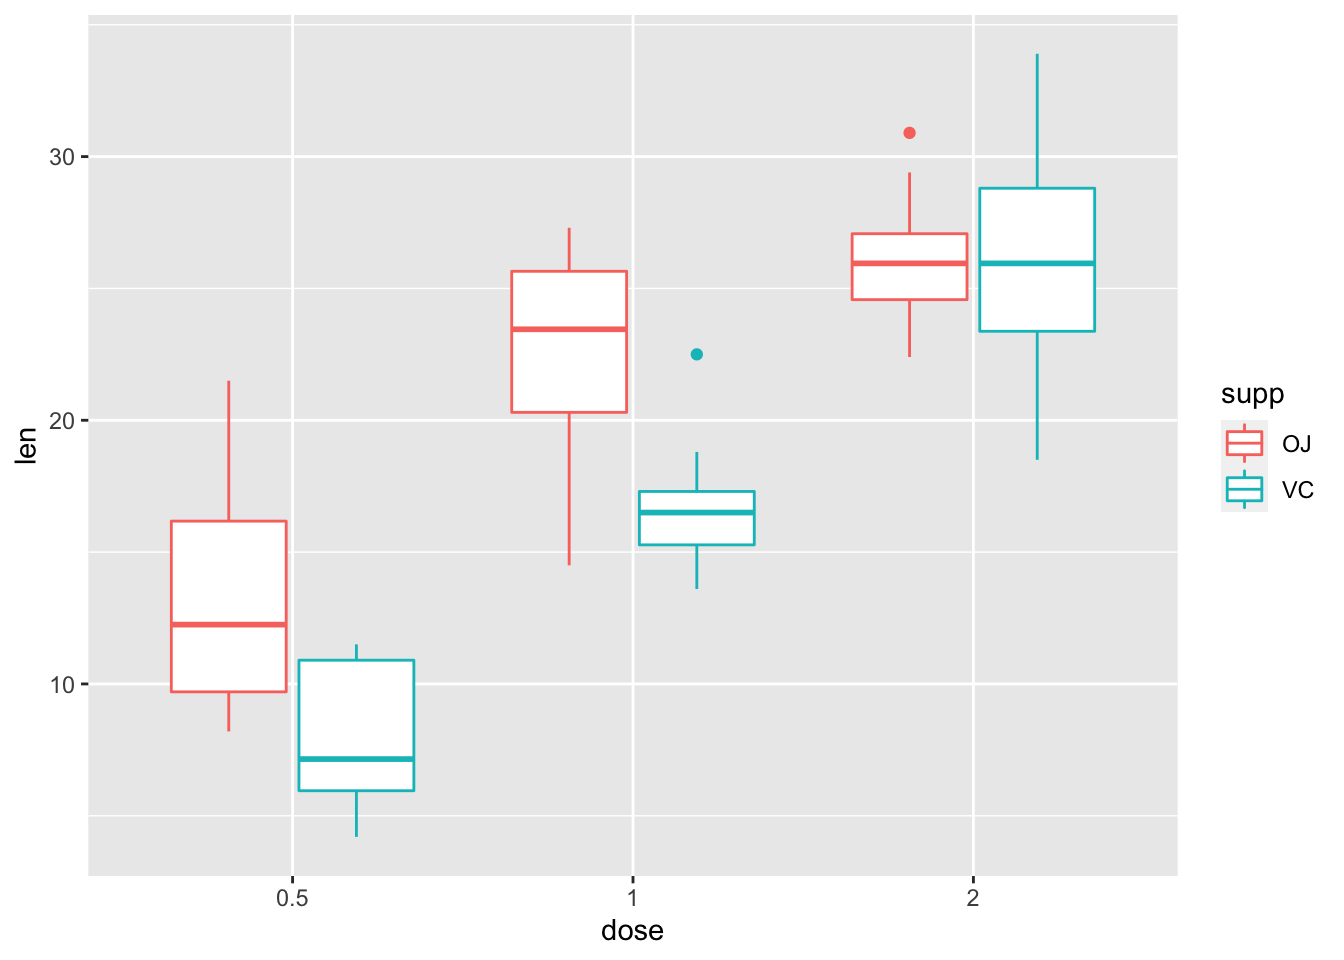
\includegraphics{r4psych_files/figure-latex/7_tooth_plot-1.pdf}

It looks like there's a main effect of dose overall, but also that supplement type probably only matters for lower doses. Let's check these using some pairwise tests. As such, perform pairwise comparisons to see where our differences lie.

\hypertarget{multiple-comparisons}{%
\subsubsection{Multiple Comparisons}\label{multiple-comparisons}}

One option is to perform multiple comparisons using Tukey Honest Significant Difference. We do this by applying the \texttt{TukeyHSD()} function to our fitted model \textbf{tooth\_aov}. Here, we also have to specify the confidence level, which is by default 95\%.

\begin{Shaded}
\begin{Highlighting}[]
\FunctionTok{TukeyHSD}\NormalTok{(tooth\_aov, }\AttributeTok{conf.level =} \FloatTok{0.95}\NormalTok{)}
\end{Highlighting}
\end{Shaded}

\begin{verbatim}
##   Tukey multiple comparisons of means
##     95% family-wise confidence level
## 
## Fit: aov(formula = len ~ supp * dose, data = tooth)
## 
## $supp
##       diff       lwr       upr     p adj
## VC-OJ -3.7 -5.579828 -1.820172 0.0002312
## 
## $dose
##         diff       lwr       upr   p adj
## 1-0.5  9.130  6.362488 11.897512 0.0e+00
## 2-0.5 15.495 12.727488 18.262512 0.0e+00
## 2-1    6.365  3.597488  9.132512 2.7e-06
## 
## $`supp:dose`
##                diff        lwr        upr     p adj
## VC:0.5-OJ:0.5 -5.25 -10.048124 -0.4518762 0.0242521
## OJ:1-OJ:0.5    9.47   4.671876 14.2681238 0.0000046
## VC:1-OJ:0.5    3.54  -1.258124  8.3381238 0.2640208
## OJ:2-OJ:0.5   12.83   8.031876 17.6281238 0.0000000
## VC:2-OJ:0.5   12.91   8.111876 17.7081238 0.0000000
## OJ:1-VC:0.5   14.72   9.921876 19.5181238 0.0000000
## VC:1-VC:0.5    8.79   3.991876 13.5881238 0.0000210
## OJ:2-VC:0.5   18.08  13.281876 22.8781238 0.0000000
## VC:2-VC:0.5   18.16  13.361876 22.9581238 0.0000000
## VC:1-OJ:1     -5.93 -10.728124 -1.1318762 0.0073930
## OJ:2-OJ:1      3.36  -1.438124  8.1581238 0.3187361
## VC:2-OJ:1      3.44  -1.358124  8.2381238 0.2936430
## OJ:2-VC:1      9.29   4.491876 14.0881238 0.0000069
## VC:2-VC:1      9.37   4.571876 14.1681238 0.0000058
## VC:2-OJ:2      0.08  -4.718124  4.8781238 1.0000000
\end{verbatim}

We get a lot of output here corresponding to every possible comparison we could ever want. We can remedy this by saving the output of TukeyHSD to an object, and selecting only the relevant information, \textbf{supp:dose}. Notice that we put this name in backticks so we can use the special character \texttt{:} without R interpreting it as something else.

\begin{Shaded}
\begin{Highlighting}[]
\NormalTok{tukey\_aov }\OtherTok{\textless{}{-}} \FunctionTok{TukeyHSD}\NormalTok{(tooth\_aov, }\AttributeTok{conf.level =} \FloatTok{0.95}\NormalTok{)}
\NormalTok{tukey\_aov}\SpecialCharTok{$}\StringTok{\textasciigrave{}}\AttributeTok{supp:dose}\StringTok{\textasciigrave{}}
\end{Highlighting}
\end{Shaded}

\begin{verbatim}
##                diff        lwr        upr        p adj
## VC:0.5-OJ:0.5 -5.25 -10.048124 -0.4518762 2.425209e-02
## OJ:1-OJ:0.5    9.47   4.671876 14.2681238 4.612304e-06
## VC:1-OJ:0.5    3.54  -1.258124  8.3381238 2.640208e-01
## OJ:2-OJ:0.5   12.83   8.031876 17.6281238 2.125153e-09
## VC:2-OJ:0.5   12.91   8.111876 17.7081238 1.769939e-09
## OJ:1-VC:0.5   14.72   9.921876 19.5181238 2.985978e-11
## VC:1-VC:0.5    8.79   3.991876 13.5881238 2.100948e-05
## OJ:2-VC:0.5   18.08  13.281876 22.8781238 4.855005e-13
## VC:2-VC:0.5   18.16  13.361876 22.9581238 4.821699e-13
## VC:1-OJ:1     -5.93 -10.728124 -1.1318762 7.393032e-03
## OJ:2-OJ:1      3.36  -1.438124  8.1581238 3.187361e-01
## VC:2-OJ:1      3.44  -1.358124  8.2381238 2.936430e-01
## OJ:2-VC:1      9.29   4.491876 14.0881238 6.908163e-06
## VC:2-VC:1      9.37   4.571876 14.1681238 5.774013e-06
## VC:2-OJ:2      0.08  -4.718124  4.8781238 1.000000e+00
\end{verbatim}

\hypertarget{multiple-regression}{%
\subsection{Multiple Regression}\label{multiple-regression}}

\hypertarget{three-level-factors}{%
\subsubsection{Three-Level Factors}\label{three-level-factors}}

If you want to see whether there's a main effect or interaction for 3 level factors, the easiest way is to simply run an ANOVA. With the \texttt{lm()} function, comparisons for the contribution of each factor in our model starts to become more difficult when we have factors with more than 2 levels. That's because we have to construct some numeric variables for these factors, and we need to perform model comparisons on a full model (with interactions) and reduced models (without) to see which model best fits our data.

To do this, we simply have to centre our two factors, with these stored as numeric variables.

\begin{Shaded}
\begin{Highlighting}[]
\CommentTok{\# code new centered variables}
\NormalTok{tooth}\SpecialCharTok{$}\NormalTok{supp\_dev }\OtherTok{\textless{}{-}}\NormalTok{ (tooth}\SpecialCharTok{$}\NormalTok{supp }\SpecialCharTok{==} \StringTok{"VC"}\NormalTok{) }\SpecialCharTok{{-}} \FunctionTok{mean}\NormalTok{(tooth}\SpecialCharTok{$}\NormalTok{supp }\SpecialCharTok{==} \StringTok{"VC"}\NormalTok{)}
\NormalTok{tooth}\SpecialCharTok{$}\NormalTok{dose\_dev\_one }\OtherTok{\textless{}{-}}\NormalTok{ (tooth}\SpecialCharTok{$}\NormalTok{dose }\SpecialCharTok{==} \StringTok{"0.5"}\NormalTok{) }\SpecialCharTok{{-}} \FunctionTok{mean}\NormalTok{(tooth}\SpecialCharTok{$}\NormalTok{dose }\SpecialCharTok{==} \StringTok{"0.5"}\NormalTok{)}
\NormalTok{tooth}\SpecialCharTok{$}\NormalTok{dose\_dev\_two }\OtherTok{\textless{}{-}}\NormalTok{ (tooth}\SpecialCharTok{$}\NormalTok{dose }\SpecialCharTok{==} \StringTok{"1"}\NormalTok{) }\SpecialCharTok{{-}} \FunctionTok{mean}\NormalTok{(tooth}\SpecialCharTok{$}\NormalTok{dose }\SpecialCharTok{==} \StringTok{"1"}\NormalTok{)}

\CommentTok{\# inspect changes}
\FunctionTok{head}\NormalTok{(tooth)}
\end{Highlighting}
\end{Shaded}

\begin{verbatim}
## # A tibble: 6 x 6
##     len supp  dose  supp_dev dose_dev_one dose_dev_two
##   <dbl> <fct> <fct>    <dbl>        <dbl>        <dbl>
## 1   4.2 VC    0.5        0.5        0.667       -0.333
## 2  11.5 VC    0.5        0.5        0.667       -0.333
## 3   7.3 VC    0.5        0.5        0.667       -0.333
## 4   5.8 VC    0.5        0.5        0.667       -0.333
## 5   6.4 VC    0.5        0.5        0.667       -0.333
## 6  10   VC    0.5        0.5        0.667       -0.333
\end{verbatim}

This centering works similarly to the contrast matrices we used before. In fact, it is often the better option if we have unbalanced data sets, as it accounts for the mismatch in the number of observations in each level of a factor. The centering used in this case is called \textbf{deviation coding} and is just like sum coding, only the parameter estimates and standard errors are half as large (but all other interpretations, e.g.~\emph{t}- and \emph{p}-values remain the same).

Now, when we fit a model with \textbf{supp\_dev}, the intercept will be the mean of the two conditions.

When it comes to fitting a 3 level factor, we need to do the same thing for only two of the levels. When we then add this to a model and test for an interaction, we test for the interaction for \textbf{supp\_dev} across both columns for our deviation coded doses.

\begin{Shaded}
\begin{Highlighting}[]
\NormalTok{tooth\_lm\_full }\OtherTok{\textless{}{-}} \FunctionTok{lm}\NormalTok{(len }\SpecialCharTok{\textasciitilde{}}\NormalTok{ supp\_dev }\SpecialCharTok{*}\NormalTok{ (dose\_dev\_one }\SpecialCharTok{+}\NormalTok{ dose\_dev\_two), }\AttributeTok{data =}\NormalTok{ tooth)}
\end{Highlighting}
\end{Shaded}

Next, we construct a reduced model, and use the \texttt{anova()} function to compare the two models against one another.

\begin{Shaded}
\begin{Highlighting}[]
\NormalTok{tooth\_lm\_reduced }\OtherTok{\textless{}{-}} \FunctionTok{lm}\NormalTok{(len }\SpecialCharTok{\textasciitilde{}}\NormalTok{ supp\_dev }\SpecialCharTok{+}\NormalTok{ (dose\_dev\_one }\SpecialCharTok{+}\NormalTok{ dose\_dev\_two), }\AttributeTok{data =}\NormalTok{ tooth)}
\FunctionTok{anova}\NormalTok{(tooth\_lm\_full, tooth\_lm\_reduced)}
\end{Highlighting}
\end{Shaded}

\begin{verbatim}
## Analysis of Variance Table
## 
## Model 1: len ~ supp_dev * (dose_dev_one + dose_dev_two)
## Model 2: len ~ supp_dev + (dose_dev_one + dose_dev_two)
##   Res.Df    RSS Df Sum of Sq     F  Pr(>F)  
## 1     54 712.11                             
## 2     56 820.43 -2   -108.32 4.107 0.02186 *
## ---
## Signif. codes:  0 '***' 0.001 '**' 0.01 '*' 0.05 '.' 0.1 ' ' 1
\end{verbatim}

This checks for how much variance is explainedby each model. As you can see, the interaction term in our model makes a significant contribution to the variance explained, so this indicates that there's an interaction in our model, and as such we should explore this.

A quick and easy way to do so is to run a number of \emph{t}-tests or linear models on subsets of the data, adjusting for the \emph{p}-values where necessary.

One way to achieve this for multifactorial designs is to create a new column which is a combination of the two factors.

\begin{Shaded}
\begin{Highlighting}[]
\CommentTok{\# create combined factor column}
\NormalTok{tooth}\SpecialCharTok{$}\NormalTok{interact }\OtherTok{\textless{}{-}} \FunctionTok{interaction}\NormalTok{(tooth}\SpecialCharTok{$}\NormalTok{supp, tooth}\SpecialCharTok{$}\NormalTok{dose)}

\CommentTok{\# check levels of our new factor}
\FunctionTok{levels}\NormalTok{(tooth}\SpecialCharTok{$}\NormalTok{interact)}
\end{Highlighting}
\end{Shaded}

\begin{verbatim}
## [1] "OJ.0.5" "VC.0.5" "OJ.1"   "VC.1"   "OJ.2"   "VC.2"
\end{verbatim}

Then we simply use the \texttt{pairwise.t.test()} function, and supply it our dependent variable and our grouping factor. This method defaults to Holm's sequential bonerroni, which is like bonferroni adjustment of \emph{p}-values, but rather than multiplying them all by the total number of comparisons, we instead multiply them incrementally, so the largest \emph{p}-value is multiplied by 1, the next smallest by 2, the next smallest by 3, etc.

\begin{Shaded}
\begin{Highlighting}[]
\FunctionTok{pairwise.t.test}\NormalTok{(tooth}\SpecialCharTok{$}\NormalTok{len, tooth}\SpecialCharTok{$}\NormalTok{interact)}
\end{Highlighting}
\end{Shaded}

\begin{verbatim}
## 
##  Pairwise comparisons using t tests with pooled SD 
## 
## data:  tooth$len and tooth$interact 
## 
##        OJ.0.5  VC.0.5  OJ.1   VC.1    OJ.2  
## VC.0.5 0.0105  -       -      -       -     
## OJ.1   3.2e-06 2.6e-11 -      -       -     
## VC.1   0.1346  1.0e-05 0.0035 -       -     
## OJ.2   1.6e-09 1.9e-14 0.1346 3.8e-06 -     
## VC.2   1.4e-09 1.7e-14 0.1346 3.6e-06 0.9609
## 
## P value adjustment method: holm
\end{verbatim}

There are other ways to automate \emph{t}-tests in R. For example, you could create a function to subset your data, apply a test, and adjust the \emph{p}-values manually, but this is not necessary here.

\hypertarget{two-level-factors}{%
\subsubsection{Two-Level Factors}\label{two-level-factors}}

Things are a lot easier when we have factors with only 2 levels. Let's assume our data had only 2 factors with 2 levels each. How would we test for main effects and interactions with a linear model?

To explore this question, we'll subset our data to only 2 levels for dose, and we'll keep only the original columns. (We use \texttt{dplyr::select} to be specific that we want select from the \texttt{dplyr} package, not another loaded package.). Remember, we want to recreate dose as a factor again so it doesn't remember our old level.

\begin{Shaded}
\begin{Highlighting}[]
\NormalTok{tooth\_sub }\OtherTok{\textless{}{-}}\NormalTok{ tooth }\SpecialCharTok{\%\textgreater{}\%} 
\NormalTok{  dplyr}\SpecialCharTok{::}\FunctionTok{select}\NormalTok{(}\DecValTok{1} \SpecialCharTok{:} \DecValTok{3}\NormalTok{) }\SpecialCharTok{\%\textgreater{}\%}
  \FunctionTok{filter}\NormalTok{(dose }\SpecialCharTok{\%in\%} \FunctionTok{c}\NormalTok{(}\FloatTok{0.5}\NormalTok{, }\DecValTok{1}\NormalTok{)) }\SpecialCharTok{\%\textgreater{}\%}
  \FunctionTok{mutate}\NormalTok{(}\AttributeTok{dose =} \FunctionTok{factor}\NormalTok{(dose))}
\end{Highlighting}
\end{Shaded}

Now, we should check our contrasts as usual.

\begin{Shaded}
\begin{Highlighting}[]
\FunctionTok{contrasts}\NormalTok{(tooth\_sub}\SpecialCharTok{$}\NormalTok{supp)}
\end{Highlighting}
\end{Shaded}

\begin{verbatim}
##    VC
## OJ  0
## VC  1
\end{verbatim}

\begin{Shaded}
\begin{Highlighting}[]
\FunctionTok{contrasts}\NormalTok{(tooth\_sub}\SpecialCharTok{$}\NormalTok{dose)}
\end{Highlighting}
\end{Shaded}

\begin{verbatim}
##     1
## 0.5 0
## 1   1
\end{verbatim}

We should make these sum coded contrasts so we can then get main effects from our model.

\begin{Shaded}
\begin{Highlighting}[]
\FunctionTok{contrasts}\NormalTok{(tooth\_sub}\SpecialCharTok{$}\NormalTok{supp) }\OtherTok{\textless{}{-}}\NormalTok{ contr.sum}
\FunctionTok{contrasts}\NormalTok{(tooth\_sub}\SpecialCharTok{$}\NormalTok{dose) }\OtherTok{\textless{}{-}}\NormalTok{ contr.sum}
\end{Highlighting}
\end{Shaded}

Then we can fit the model again.

\begin{Shaded}
\begin{Highlighting}[]
\NormalTok{tooth\_sub\_lm }\OtherTok{\textless{}{-}} \FunctionTok{lm}\NormalTok{(len }\SpecialCharTok{\textasciitilde{}}\NormalTok{ supp }\SpecialCharTok{*}\NormalTok{ dose, }\AttributeTok{data =}\NormalTok{ tooth\_sub)}
\FunctionTok{summary}\NormalTok{(tooth\_sub\_lm)}
\end{Highlighting}
\end{Shaded}

\begin{verbatim}
## 
## Call:
## lm(formula = len ~ supp * dose, data = tooth_sub)
## 
## Residuals:
##    Min     1Q Median     3Q    Max 
##  -8.20  -2.72  -0.27   2.65   8.27 
## 
## Coefficients:
##             Estimate Std. Error t value Pr(>|t|)    
## (Intercept)  15.1700     0.5537  27.397  < 2e-16 ***
## supp1         2.7950     0.5537   5.048 1.30e-05 ***
## dose1        -4.5650     0.5537  -8.244 8.25e-10 ***
## supp1:dose1  -0.1700     0.5537  -0.307    0.761    
## ---
## Signif. codes:  0 '***' 0.001 '**' 0.01 '*' 0.05 '.' 0.1 ' ' 1
## 
## Residual standard error: 3.502 on 36 degrees of freedom
## Multiple R-squared:  0.7221, Adjusted R-squared:  0.6989 
## F-statistic: 31.18 on 3 and 36 DF,  p-value: 4.098e-10
\end{verbatim}

The only thing to note here is that we've used sum coding other than deviation coding with the 3-level case. Our interpretation of effects stays the same here, only our paramter estimates and standard errors will be twice as large with sum coding when compared to deviation coding.

If your factors are not sum/deviation coded, then you won't observe main effects. So we can test for the effect of dose at the first level of supplement as follows:

\begin{Shaded}
\begin{Highlighting}[]
\FunctionTok{contrasts}\NormalTok{(tooth\_sub}\SpecialCharTok{$}\NormalTok{supp) }\OtherTok{\textless{}{-}}\NormalTok{ contr.treatment}
\FunctionTok{contrasts}\NormalTok{(tooth\_sub}\SpecialCharTok{$}\NormalTok{supp)}
\end{Highlighting}
\end{Shaded}

\begin{verbatim}
##    2
## OJ 0
## VC 1
\end{verbatim}

OJ will now be our reference value for the intercept. Additionally, the effect of dose will be compared at this intercept value, so we now have simple effects of dose, and main effects of supplement. The interpretation for our interaction terms remains the same regardless of our coding approach.

\begin{Shaded}
\begin{Highlighting}[]
\NormalTok{tooth\_sub\_lm2 }\OtherTok{\textless{}{-}} \FunctionTok{lm}\NormalTok{(len }\SpecialCharTok{\textasciitilde{}}\NormalTok{ supp }\SpecialCharTok{*}\NormalTok{ dose, }\AttributeTok{data =}\NormalTok{ tooth\_sub)}
\FunctionTok{summary}\NormalTok{(tooth\_sub\_lm2)}
\end{Highlighting}
\end{Shaded}

\begin{verbatim}
## 
## Call:
## lm(formula = len ~ supp * dose, data = tooth_sub)
## 
## Residuals:
##    Min     1Q Median     3Q    Max 
##  -8.20  -2.72  -0.27   2.65   8.27 
## 
## Coefficients:
##             Estimate Std. Error t value Pr(>|t|)    
## (Intercept)  17.9650     0.7831  22.942  < 2e-16 ***
## supp2        -5.5900     1.1074  -5.048 1.30e-05 ***
## dose1        -4.7350     0.7831  -6.047 6.02e-07 ***
## supp2:dose1   0.3400     1.1074   0.307    0.761    
## ---
## Signif. codes:  0 '***' 0.001 '**' 0.01 '*' 0.05 '.' 0.1 ' ' 1
## 
## Residual standard error: 3.502 on 36 degrees of freedom
## Multiple R-squared:  0.7221, Adjusted R-squared:  0.6989 
## F-statistic: 31.18 on 3 and 36 DF,  p-value: 4.098e-10
\end{verbatim}

\hypertarget{mixed-analyses}{%
\section{Mixed Analyses}\label{mixed-analyses}}

Mixed factorial analyses are just a special form of factorial analyses. Here, one factor is between subjects and another factor is within subjects. Here, we'll create some new data based on our smoking data that reflects a mixed design.

\begin{Shaded}
\begin{Highlighting}[]
\CommentTok{\# set parameters}
\FunctionTok{set.seed}\NormalTok{(}\DecValTok{1000}\NormalTok{)}
\NormalTok{means }\OtherTok{\textless{}{-}} \FunctionTok{rep}\NormalTok{(}\FunctionTok{c}\NormalTok{(}\DecValTok{80}\NormalTok{, }\DecValTok{85}\NormalTok{), }\DecValTok{100}\NormalTok{)}
\NormalTok{sds }\OtherTok{\textless{}{-}} \FunctionTok{rep}\NormalTok{(}\FunctionTok{c}\NormalTok{(}\DecValTok{5}\NormalTok{, }\DecValTok{5}\NormalTok{, }\DecValTok{7}\NormalTok{), }\DecValTok{100}\NormalTok{)}
\NormalTok{cond }\OtherTok{\textless{}{-}} \FunctionTok{rep}\NormalTok{(}\FunctionTok{c}\NormalTok{(}\StringTok{"control"}\NormalTok{, }\StringTok{"drug\_one"}\NormalTok{), }\DecValTok{100}\NormalTok{)}
\NormalTok{subject }\OtherTok{\textless{}{-}} \FunctionTok{seq}\NormalTok{(}\DecValTok{1}\SpecialCharTok{:}\DecValTok{200}\NormalTok{)}

\CommentTok{\# simulate data}
\NormalTok{smoking\_dat\_extra }\OtherTok{\textless{}{-}} \FunctionTok{tibble}\NormalTok{(}
  \AttributeTok{subject =}\NormalTok{ subject,}
  \AttributeTok{cond =} \FunctionTok{as.factor}\NormalTok{(cond),}
  \AttributeTok{time\_one =} \FunctionTok{rnorm}\NormalTok{(}\AttributeTok{n =} \DecValTok{200}\NormalTok{, }\AttributeTok{mean =}\NormalTok{ means, }\AttributeTok{sd =}\NormalTok{ sds),}
  \AttributeTok{time\_two =}\NormalTok{ time\_one }\SpecialCharTok{+} \FunctionTok{rnorm}\NormalTok{(}\AttributeTok{n =} \DecValTok{200}\NormalTok{, }\AttributeTok{mean =} \DecValTok{5}\NormalTok{, }\AttributeTok{sd =}\NormalTok{ sds)}
\NormalTok{  ) }\SpecialCharTok{\%\textgreater{}\%}
  \FunctionTok{gather}\NormalTok{(}\AttributeTok{key =}\NormalTok{ test\_time,}
         \AttributeTok{value =}\NormalTok{ recovery,}
         \DecValTok{3}\SpecialCharTok{:}\DecValTok{4}
\NormalTok{         ) }\SpecialCharTok{\%\textgreater{}\%}
  \FunctionTok{mutate}\NormalTok{(}\AttributeTok{test\_time =} \FunctionTok{as.factor}\NormalTok{(test\_time)) }\SpecialCharTok{\%\textgreater{}\%}
  \FunctionTok{arrange}\NormalTok{(subject)}

\CommentTok{\# view the data}
\NormalTok{smoking\_dat\_extra}
\end{Highlighting}
\end{Shaded}

\begin{verbatim}
## # A tibble: 400 x 4
##    subject cond     test_time recovery
##      <int> <fct>    <fct>        <dbl>
##  1       1 control  time_one      77.8
##  2       1 control  time_two      87.4
##  3       2 drug_one time_one      79.0
##  4       2 drug_one time_two      87.6
##  5       3 control  time_one      80.3
##  6       3 control  time_two      73.5
##  7       4 drug_one time_one      88.2
##  8       4 drug_one time_two      92.0
##  9       5 control  time_one      76.1
## 10       5 control  time_two      77.8
## # ... with 390 more rows
\end{verbatim}

Now our smoking data is a little more complex, and a simpler in parts. For one, we now only have two drugs, the placebo (control) or drug\_one. However now we've tested people at two time points to see if time plays a factor in their recovery.

\hypertarget{mixed-linear-models}{%
\subsection{Mixed Linear Models}\label{mixed-linear-models}}

First, we'll make sure our factors are sum coded so that we can obtain main effects of both factors.

\begin{Shaded}
\begin{Highlighting}[]
\FunctionTok{contrasts}\NormalTok{(smoking\_dat\_extra}\SpecialCharTok{$}\NormalTok{cond) }\OtherTok{\textless{}{-}}\NormalTok{ contr.sum}
\FunctionTok{contrasts}\NormalTok{(smoking\_dat\_extra}\SpecialCharTok{$}\NormalTok{test\_time) }\OtherTok{\textless{}{-}}\NormalTok{ contr.sum}
\end{Highlighting}
\end{Shaded}

Then, we'll refit the model as before.

\begin{Shaded}
\begin{Highlighting}[]
\NormalTok{mixed\_lm }\OtherTok{\textless{}{-}} \FunctionTok{lm}\NormalTok{(recovery }\SpecialCharTok{\textasciitilde{}}\NormalTok{ cond }\SpecialCharTok{*}\NormalTok{ test\_time, }
                 \AttributeTok{data =}\NormalTok{ smoking\_dat\_extra)}
\FunctionTok{summary}\NormalTok{(mixed\_lm)}
\end{Highlighting}
\end{Shaded}

\begin{verbatim}
## 
## Call:
## lm(formula = recovery ~ cond * test_time, data = smoking_dat_extra)
## 
## Residuals:
##      Min       1Q   Median       3Q      Max 
## -23.7613  -3.8794   0.4193   4.3061  20.2756 
## 
## Coefficients:
##                  Estimate Std. Error t value Pr(>|t|)    
## (Intercept)       85.3816     0.3370 253.385  < 2e-16 ***
## cond1             -2.6232     0.3370  -7.785 6.15e-14 ***
## test_time1        -2.5064     0.3370  -7.438 6.40e-13 ***
## cond1:test_time1   0.0612     0.3370   0.182    0.856    
## ---
## Signif. codes:  0 '***' 0.001 '**' 0.01 '*' 0.05 '.' 0.1 ' ' 1
## 
## Residual standard error: 6.739 on 396 degrees of freedom
## Multiple R-squared:  0.2265, Adjusted R-squared:  0.2206 
## F-statistic: 38.65 on 3 and 396 DF,  p-value: < 2.2e-16
\end{verbatim}

Now our intercept corresponds to the grand mean, and our effects of condition and test time are main effects of these two factors. The interaction again tells us that we need to explore the data. For this, we'd just use the same methods from above.

However, this model doesn't account for the dependencies between subjects and their scores. In order to do this, we should use the `aov()' function, which is simply a wrapper for the linear model, but allows for accounting for between-subjects factors. Alternatively, we can improve on our linear models by making them account for subjects-based effects, and we'll cover this in later sessions on \textbf{mixed effects modelling}.

\hypertarget{mixed-anova}{%
\subsection{Mixed ANOVA}\label{mixed-anova}}

With a mixed ANOVA, we are simply just including an error term for our within-subjects factor. We do this in the same way as for within-subjects ANOVAs, only leaving the error term off the between-subjects factor.

In this case, subjects take part in both test time conditions, so we need to nest this within our data.

\begin{Shaded}
\begin{Highlighting}[]
\NormalTok{mixed\_aov }\OtherTok{\textless{}{-}} \FunctionTok{aov}\NormalTok{(recovery }\SpecialCharTok{\textasciitilde{}}\NormalTok{ cond }\SpecialCharTok{*}\NormalTok{ test\_time }\SpecialCharTok{+} 
                   \FunctionTok{Error}\NormalTok{(subject}\SpecialCharTok{/}\NormalTok{test\_time), }
                 \AttributeTok{data =}\NormalTok{ smoking\_dat\_extra)}
\FunctionTok{summary}\NormalTok{(mixed\_aov)}
\end{Highlighting}
\end{Shaded}

\begin{verbatim}
## 
## Error: subject
##      Df Sum Sq Mean Sq
## cond  1  261.2   261.2
## 
## Error: subject:test_time
##           Df Sum Sq Mean Sq
## test_time  1   2077    2077
## 
## Error: Within
##                 Df Sum Sq Mean Sq F value   Pr(>F)    
## cond             1   2738  2738.1  60.877 5.51e-14 ***
## test_time        1    454   453.9  10.091  0.00161 ** 
## cond:test_time   1      1     1.4   0.031  0.85956    
## Residuals      394  17721    45.0                     
## ---
## Signif. codes:  0 '***' 0.001 '**' 0.01 '*' 0.05 '.' 0.1 ' ' 1
\end{verbatim}

Now we have our main effects of condition, test time, and the interaction between them.

\hypertarget{a-note-on-sum-of-squares}{%
\section{A Note on Sum of Squares}\label{a-note-on-sum-of-squares}}

In some cases, you might notice that the output of your ANOVA models does not correspond to the output of that from SPSS or other statistical packages. That's because R defaults to type-I sum of squares, and SPSS defaults to type-III sum of squares.

Put simply, when you have an unbalanced design, such as when you have an unequal number of participants in each group, the way in which the sum of squares is calculated will affect the output and interpretation of your ANOVA.

With type-I sum of squares, which is R's default, the order in which you specify factors in your model will determine how much variance is explained by each factor. With type-I sum of squares, the terms are considered in the model in a sequential order. Take a look at this in action below. We'll use the \textbf{tooth\_sub} data from before, but we'll remove the first observation.

\begin{Shaded}
\begin{Highlighting}[]
\NormalTok{tooth\_sub\_unbalanced }\OtherTok{\textless{}{-}}\NormalTok{ tooth\_sub[}\DecValTok{2}\SpecialCharTok{:}\DecValTok{40}\NormalTok{,]}
\end{Highlighting}
\end{Shaded}

\begin{Shaded}
\begin{Highlighting}[]
\NormalTok{supp\_first }\OtherTok{\textless{}{-}} \FunctionTok{aov}\NormalTok{(len }\SpecialCharTok{\textasciitilde{}}\NormalTok{ supp }\SpecialCharTok{*}\NormalTok{ dose, }\AttributeTok{data =}\NormalTok{ tooth\_sub\_unbalanced)}
\FunctionTok{summary}\NormalTok{(supp\_first)}
\end{Highlighting}
\end{Shaded}

\begin{verbatim}
##             Df Sum Sq Mean Sq F value   Pr(>F)    
## supp         1  259.4   259.4  21.331 5.05e-05 ***
## dose         1  777.3   777.3  63.920 2.09e-09 ***
## supp:dose    1    2.9     2.9   0.242    0.626    
## Residuals   35  425.6    12.2                     
## ---
## Signif. codes:  0 '***' 0.001 '**' 0.01 '*' 0.05 '.' 0.1 ' ' 1
\end{verbatim}

\begin{Shaded}
\begin{Highlighting}[]
\NormalTok{dose\_first }\OtherTok{\textless{}{-}} \FunctionTok{aov}\NormalTok{(len }\SpecialCharTok{\textasciitilde{}}\NormalTok{ dose }\SpecialCharTok{*}\NormalTok{ supp, }\AttributeTok{data =}\NormalTok{ tooth\_sub\_unbalanced)}
\FunctionTok{summary}\NormalTok{(dose\_first)}
\end{Highlighting}
\end{Shaded}

\begin{verbatim}
##             Df Sum Sq Mean Sq F value   Pr(>F)    
## dose         1  753.3   753.3  61.948 2.98e-09 ***
## supp         1  283.4   283.4  23.304 2.70e-05 ***
## dose:supp    1    2.9     2.9   0.242    0.626    
## Residuals   35  425.6    12.2                     
## ---
## Signif. codes:  0 '***' 0.001 '**' 0.01 '*' 0.05 '.' 0.1 ' ' 1
\end{verbatim}

Here, you can see that the sum of squares, and consequently the F-values (and hence \emph{p}-values) differ depending on the order in which we entered our factors in the model. What happens is that the first term in the model is evaluated first, and any variance explained that is shared by dose and supp is instead given to the first term in the model. Therefore, we shouldn't really use type-I sum of squares unless our two factors are entirely independent of one-another.

Alternatively, we have type-II sum of squares, which evaluates the main effects of your factors while ignoring the variance explained by interaction terms. Crucially, if you do have an interaction, type-II sum of squares will not accurately reflect the variance explained by the interaction as that variance is given over to the main effect terms. Crucially, the coding scheme used for type-II sum of squares does not matter.

In Psychology, we typically use type-III sum of squares, where main effects are computed while taking the interaction into account. This method is recommended for unbalanced designs, although there is some debate on this. However, type-III sum of squares only work with orthogonal contrast matrices (i.e.~sum/helmert coding), so make sure you pay attention to how you've coded your factors prior to fitting a model.

The way to refit our model with type-III sum of squares is to use the \texttt{Anova()} (notice the capital A) function from the \textbf{car} package, specifying the type for your sum of squares. This function takes the object of your model fitted by \texttt{aov()} and the type for the sum of squares you would like to compute. Note that this function defaults to type-II sum of squares, so we need to be specific in our function call.

First, install this package and load it, then run the function on the two model fits from above.

\begin{Shaded}
\begin{Highlighting}[]
\CommentTok{\# install.packages("car") \# install once per machine}
\FunctionTok{library}\NormalTok{(car) }\CommentTok{\# load each time you open R}
\end{Highlighting}
\end{Shaded}

\begin{verbatim}
## Loading required package: carData
\end{verbatim}

\begin{verbatim}
## 
## Attaching package: 'car'
\end{verbatim}

\begin{verbatim}
## The following object is masked from 'package:dplyr':
## 
##     recode
\end{verbatim}

\begin{verbatim}
## The following object is masked from 'package:purrr':
## 
##     some
\end{verbatim}

\begin{Shaded}
\begin{Highlighting}[]
\FunctionTok{Anova}\NormalTok{(supp\_first, }\AttributeTok{type =} \StringTok{"III"}\NormalTok{)}
\end{Highlighting}
\end{Shaded}

\begin{verbatim}
## Anova Table (Type III tests)
## 
## Response: len
##             Sum Sq Df F value    Pr(>F)    
## (Intercept) 6454.8  1 530.797 < 2.2e-16 ***
## supp         281.6  1  23.158 2.824e-05 ***
## dose         448.4  1  36.873 6.201e-07 ***
## supp:dose      2.9  1   0.242    0.6258    
## Residuals    425.6 35                      
## ---
## Signif. codes:  0 '***' 0.001 '**' 0.01 '*' 0.05 '.' 0.1 ' ' 1
\end{verbatim}

\begin{Shaded}
\begin{Highlighting}[]
\FunctionTok{Anova}\NormalTok{(dose\_first, }\AttributeTok{type =} \StringTok{"III"}\NormalTok{)}
\end{Highlighting}
\end{Shaded}

\begin{verbatim}
## Anova Table (Type III tests)
## 
## Response: len
##             Sum Sq Df F value    Pr(>F)    
## (Intercept) 6454.8  1 530.797 < 2.2e-16 ***
## dose         448.4  1  36.873 6.201e-07 ***
## supp         281.6  1  23.158 2.824e-05 ***
## dose:supp      2.9  1   0.242    0.6258    
## Residuals    425.6 35                      
## ---
## Signif. codes:  0 '***' 0.001 '**' 0.01 '*' 0.05 '.' 0.1 ' ' 1
\end{verbatim}

As you can see, the results of both analyses are equivalent for the unbalanced data set using this function.

As a final note, in all cases we should check that the tests we run meet the assumptions of said test. For factorial ANOVAs, this means checking the previous assumptions for a one-way ANOVA, while also checking for a lack of multicollinearity between the factors in the design, which we won't cover here.

\hypertarget{exercises-6}{%
\section{Exercises}\label{exercises-6}}

For these exercises, we will look at the core concepts from this lesson. Here, we'll use a simulated data set that's saved as a .csv in the inputs folder.

If you don't have access to these, please \href{https://github.com/gpwilliams/r4psych}{download the repository from GitHub} and open the \textbf{lesson\_materials} folder. Open the relevant folder for this lesson. If you work out of the file \textbf{07\_advanced\_statistical\_tests.Rmd} the code below will work to load the data set. If this fails then quit R and open it up from the .Rmd file above so your working directory is in the correct folder.

\begin{Shaded}
\begin{Highlighting}[]
\FunctionTok{library}\NormalTok{(tidyverse)}
\CommentTok{\# install.packages("car") \# install if necessary (once per machine)}
\FunctionTok{library}\NormalTok{(car)}
\FunctionTok{library}\NormalTok{(ggpirate)}
\end{Highlighting}
\end{Shaded}

Next, we'll load the data set for this exercise.

\begin{Shaded}
\begin{Highlighting}[]
\NormalTok{factorial\_data }\OtherTok{\textless{}{-}} \FunctionTok{read\_csv}\NormalTok{(}\StringTok{"inputs/factorial\_data.csv"}\NormalTok{)}
\end{Highlighting}
\end{Shaded}

\hypertarget{question-1-6}{%
\subsection{Question 1}\label{question-1-6}}

Aggregate the data by subject such that you have 1 score per subject for the mean of the column Y across both A and B columns. Call the Y column mean\_Y. Assign this to the object \textbf{data\_agg}.

\hypertarget{question-2-6}{%
\subsection{Question 2}\label{question-2-6}}

Generate summary statistics for the data set and a pirate plot of the data set. We want means, SDs, and ns for the table of summary statistics.

\hypertarget{question-3-6}{%
\subsection{Question 3}\label{question-3-6}}

Define your contrasts such that you have main effects and interactions from any model fits. You may need to check your data types for this to work properly.
\emph{Hint}: use \texttt{mutate()} after the \texttt{ungroup()} function

\hypertarget{question-4-6}{%
\subsection{Question 4}\label{question-4-6}}

Fit the data set checking for all main effects and interactions.

\hypertarget{question-5-6}{%
\subsection{Question 5}\label{question-5-6}}

Refit your model from Question 5 using type-III sum of squares. Did that make any difference to your sum of squares? Why or why not?

\hypertarget{question-6-6}{%
\subsection{Question 6}\label{question-6-6}}

Explore the parameter estimates from your ANOVA model, and briefly report your findings in text (1 sentence max).

\hypertarget{simulation-and-calculating-power}{%
\chapter{Simulation and Calculating Power}\label{simulation-and-calculating-power}}

In this session we'll cover how to simualte data to improve our statistical inferences. We'll use simulation to perform power analyses, and to understand more about how \emph{p}-values work. Finally, we'll look at how you can calculate power easily and quickly in several pre-existing packages and functions in R.

Specifically, we'll cover:

\begin{itemize}
\tightlist
\item
  simulating data in R
\item
  simulation-based power analyses
\item
  packages for power analysis
\end{itemize}

\hypertarget{getting-started-5}{%
\section{Getting Started}\label{getting-started-5}}

As always, we first need to load the \texttt{tidyverse} set of package to perform the data manipulation for this chapter.

\begin{Shaded}
\begin{Highlighting}[]
\CommentTok{\# load packages}
\FunctionTok{library}\NormalTok{(tidyverse)}
\end{Highlighting}
\end{Shaded}

\hypertarget{simulating-data}{%
\section{Simulating Data}\label{simulating-data}}

First off, we'll explore different ways to simulate data using some of the basic functions in R. We'll look at randomly sampling data that adheres to the following distributions:

\begin{itemize}
\tightlist
\item
  Uniform, using \texttt{runif()} (read: \textbf{r}andom \textbf{unif}orm)
\item
  Normal, using \texttt{rnorm()} (read: \textbf{r}andom \textbf{norm}al )
\item
  Binomial, using \texttt{rbinom()} (read: \textbf{r}andom \textbf{binom}ial)
\end{itemize}

Additionally, we'll look at randomly sampling data with and without replacement, and how we can determine bias in our sampling procedure by defining the probability with which items should be sampled.

We'll look at sampling data following these distributions as this provides us with a better understanding of our data, and equips us with the means to evaluate our research plans prior to the expensive (in terms of time and money) procedure of testing. Put simply, simulating data is useful because it allows us to do things like calculate power for simple and complex experimental designs, and to observe when participants are performing to change in tasks.

\hypertarget{the-uniform-distribution}{%
\subsection{The Uniform Distribution}\label{the-uniform-distribution}}

With the uniform distribution, we sample numbers such that all values are equally likely to be drawn from our range. Try this out a few times:

\begin{Shaded}
\begin{Highlighting}[]
\FunctionTok{runif}\NormalTok{(}\AttributeTok{n =} \DecValTok{5}\NormalTok{, }\AttributeTok{min =} \DecValTok{1}\NormalTok{, }\AttributeTok{max =} \DecValTok{10}\NormalTok{)}
\end{Highlighting}
\end{Shaded}

\begin{verbatim}
## [1] 3.300586 2.342055 4.873663 9.191708 5.319560
\end{verbatim}

In all likelihood, you should get different numbers to those above, but your numbers will all be between 1 and 10 (excluding these two values). You can increase the amount of numbers sampled by changing \texttt{n} to anything else. For example, try this:

\begin{Shaded}
\begin{Highlighting}[]
\FunctionTok{runif}\NormalTok{(}\AttributeTok{n =} \DecValTok{10}\NormalTok{, }\AttributeTok{min =} \DecValTok{1}\NormalTok{, }\AttributeTok{max =} \DecValTok{10}\NormalTok{)}
\end{Highlighting}
\end{Shaded}

\begin{verbatim}
##  [1] 8.011183 5.748096 1.380451 7.302121 5.467758 6.987622 2.161111 5.345088
##  [9] 5.670862 4.214587
\end{verbatim}

Now we have 10 numbers between 1 and 10.

Finally, we can change the minimum and maximum values, or the range of values we want to sample from. Let's sample 10 numbers from between 0 and 1.

\begin{Shaded}
\begin{Highlighting}[]
\FunctionTok{runif}\NormalTok{(}\AttributeTok{n =} \DecValTok{10}\NormalTok{, }\AttributeTok{min =} \DecValTok{0}\NormalTok{, }\AttributeTok{max =} \DecValTok{1}\NormalTok{)}
\end{Highlighting}
\end{Shaded}

\begin{verbatim}
##  [1] 0.90863606 0.60394266 0.78368223 0.47517589 0.03186038 0.51023136
##  [7] 0.51073424 0.58464829 0.76034355 0.08140943
\end{verbatim}

What happens if we calculate the mean from 10 samples from a uniform distribution? What about 100, 1000, or even 10000?

\begin{Shaded}
\begin{Highlighting}[]
\FunctionTok{runif}\NormalTok{(}\AttributeTok{n =} \DecValTok{10}\NormalTok{, }\AttributeTok{min =} \DecValTok{0}\NormalTok{, }\AttributeTok{max =} \DecValTok{1}\NormalTok{) }\SpecialCharTok{\%\textgreater{}\%} \FunctionTok{mean}\NormalTok{()}
\end{Highlighting}
\end{Shaded}

\begin{verbatim}
## [1] 0.4962173
\end{verbatim}

\begin{Shaded}
\begin{Highlighting}[]
\FunctionTok{runif}\NormalTok{(}\AttributeTok{n =} \DecValTok{100}\NormalTok{, }\AttributeTok{min =} \DecValTok{0}\NormalTok{, }\AttributeTok{max =} \DecValTok{1}\NormalTok{) }\SpecialCharTok{\%\textgreater{}\%} \FunctionTok{mean}\NormalTok{()}
\end{Highlighting}
\end{Shaded}

\begin{verbatim}
## [1] 0.4754119
\end{verbatim}

\begin{Shaded}
\begin{Highlighting}[]
\FunctionTok{runif}\NormalTok{(}\AttributeTok{n =} \DecValTok{1000}\NormalTok{, }\AttributeTok{min =} \DecValTok{0}\NormalTok{, }\AttributeTok{max =} \DecValTok{1}\NormalTok{) }\SpecialCharTok{\%\textgreater{}\%} \FunctionTok{mean}\NormalTok{()}
\end{Highlighting}
\end{Shaded}

\begin{verbatim}
## [1] 0.4878579
\end{verbatim}

\begin{Shaded}
\begin{Highlighting}[]
\FunctionTok{runif}\NormalTok{(}\AttributeTok{n =} \DecValTok{10000}\NormalTok{, }\AttributeTok{min =} \DecValTok{0}\NormalTok{, }\AttributeTok{max =} \DecValTok{1}\NormalTok{) }\SpecialCharTok{\%\textgreater{}\%} \FunctionTok{mean}\NormalTok{()}
\end{Highlighting}
\end{Shaded}

\begin{verbatim}
## [1] 0.5000408
\end{verbatim}

As you can see, as we draw more samples, the mean of these samples better represents the true distribution of our sampling procedure. Think about how this could impact your studies. With small sample sizes, we're likely to get skewed data that tends towards the extremes.

\hypertarget{the-normal-distribution}{%
\subsection{The Normal Distribution}\label{the-normal-distribution}}

Alternatively, we can sample continuous data from the normal distribution. We might use this to generate data on a continuous scale with a normal distribution in the population, such as the height and weight of a participant, or even their IQ.

To do this, we use the \texttt{rnorm()} function. You may have noticed me doing this when creating data for the previous sessions, and that's with good reason; we often fit our data with models that assume a normal distribution of our variables, and so creating data with this assumed distribution often meets the assumptions of the tests we'd like to run.

This sampling function provides us with a good range of values if we know (or can guess at) the mean and standard deviation of a sample from a population. Let's see how this works. Below, we'll sample some data from a population where we know the mean and standard deviation; the IQ test. Here, the mean is 100 and the standard deviation is 15. Let's go ahead and sample 10 people from this population.

\begin{Shaded}
\begin{Highlighting}[]
\FunctionTok{rnorm}\NormalTok{(}\AttributeTok{n =} \DecValTok{10}\NormalTok{, }\AttributeTok{mean =} \DecValTok{100}\NormalTok{, }\AttributeTok{sd =} \DecValTok{15}\NormalTok{)}
\end{Highlighting}
\end{Shaded}

\begin{verbatim}
##  [1]  82.16277  99.75992 128.28859  76.65559  73.06495  97.49910  96.44725
##  [8] 102.10636  91.52518 125.11196
\end{verbatim}

OK, we have a good range of values for our IQ test here, but as before, with a small sample size our distribution will be skewed. Let's observe how this plays out with a density plot. (Here, I'm being lazy and not defining \texttt{mapping\ =\ aes()}, as ggplot understands that what we put in \texttt{aes()} will be mapped to the data/plot.)

\begin{Shaded}
\begin{Highlighting}[]
\FunctionTok{set.seed}\NormalTok{(}\DecValTok{5}\NormalTok{)}
\NormalTok{small\_samp }\OtherTok{\textless{}{-}} \FunctionTok{rnorm}\NormalTok{(}\AttributeTok{n =} \DecValTok{100}\NormalTok{, }\AttributeTok{mean =} \DecValTok{100}\NormalTok{, }\AttributeTok{sd =} \DecValTok{15}\NormalTok{)}
\NormalTok{large\_samp }\OtherTok{\textless{}{-}} \FunctionTok{rnorm}\NormalTok{(}\AttributeTok{n =} \DecValTok{1000}\NormalTok{, }\AttributeTok{mean =} \DecValTok{100}\NormalTok{, }\AttributeTok{sd =} \DecValTok{15}\NormalTok{)}

\FunctionTok{ggplot}\NormalTok{() }\SpecialCharTok{+} \FunctionTok{geom\_density}\NormalTok{(}\FunctionTok{aes}\NormalTok{(small\_samp)) }\SpecialCharTok{+} \FunctionTok{coord\_cartesian}\NormalTok{(}\AttributeTok{x =} \FunctionTok{c}\NormalTok{(}\DecValTok{50}\NormalTok{, }\DecValTok{150}\NormalTok{))}
\end{Highlighting}
\end{Shaded}

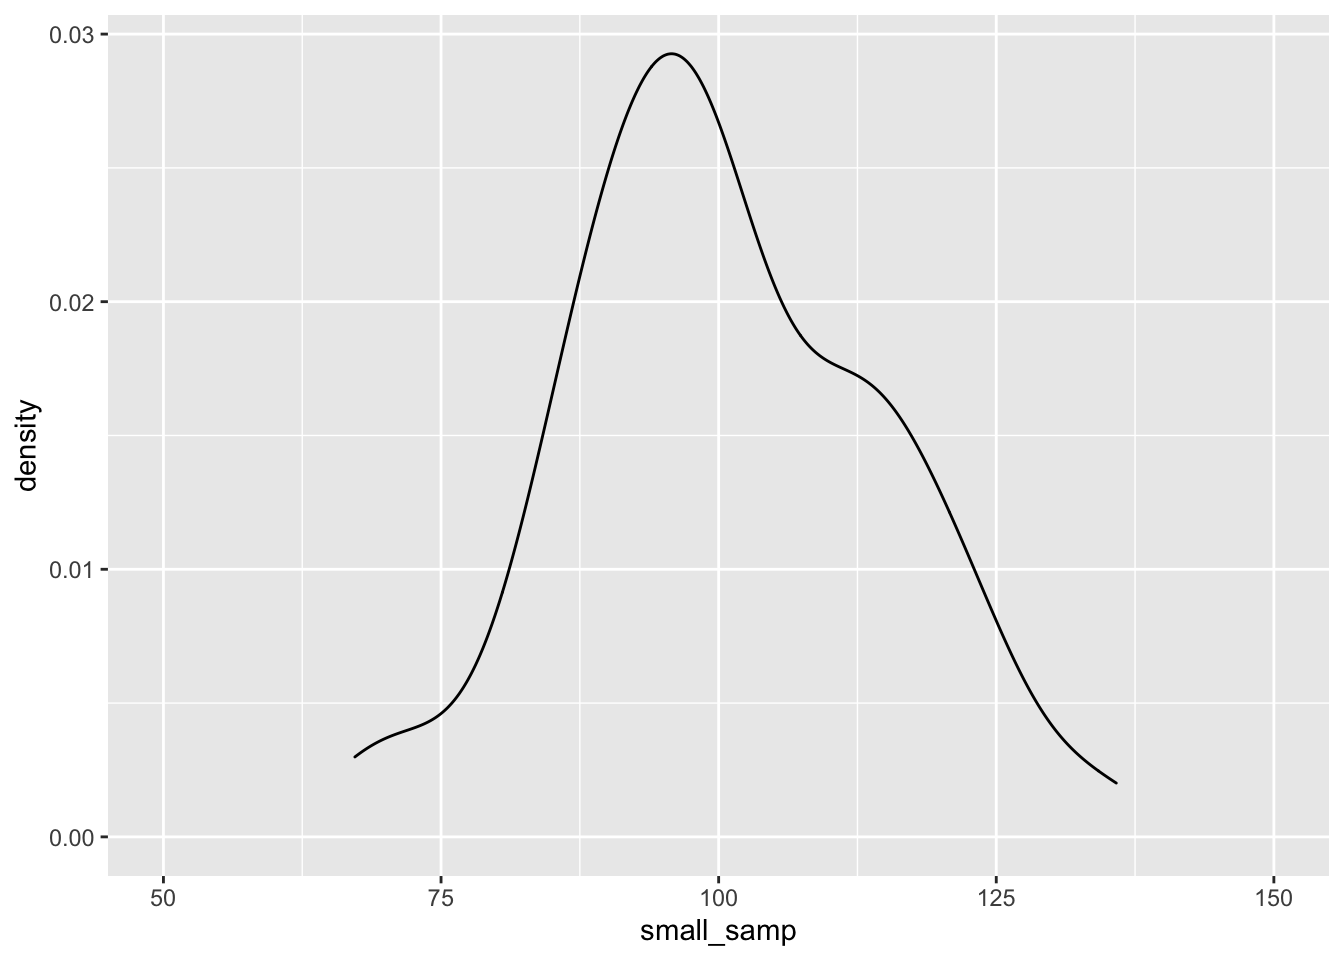
\includegraphics{r4psych_files/figure-latex/8_norm_sample_sizes-1.pdf}

\begin{Shaded}
\begin{Highlighting}[]
\FunctionTok{ggplot}\NormalTok{() }\SpecialCharTok{+} \FunctionTok{geom\_density}\NormalTok{(}\FunctionTok{aes}\NormalTok{(large\_samp)) }\SpecialCharTok{+} \FunctionTok{coord\_cartesian}\NormalTok{(}\AttributeTok{x =} \FunctionTok{c}\NormalTok{(}\DecValTok{50}\NormalTok{, }\DecValTok{150}\NormalTok{))}
\end{Highlighting}
\end{Shaded}

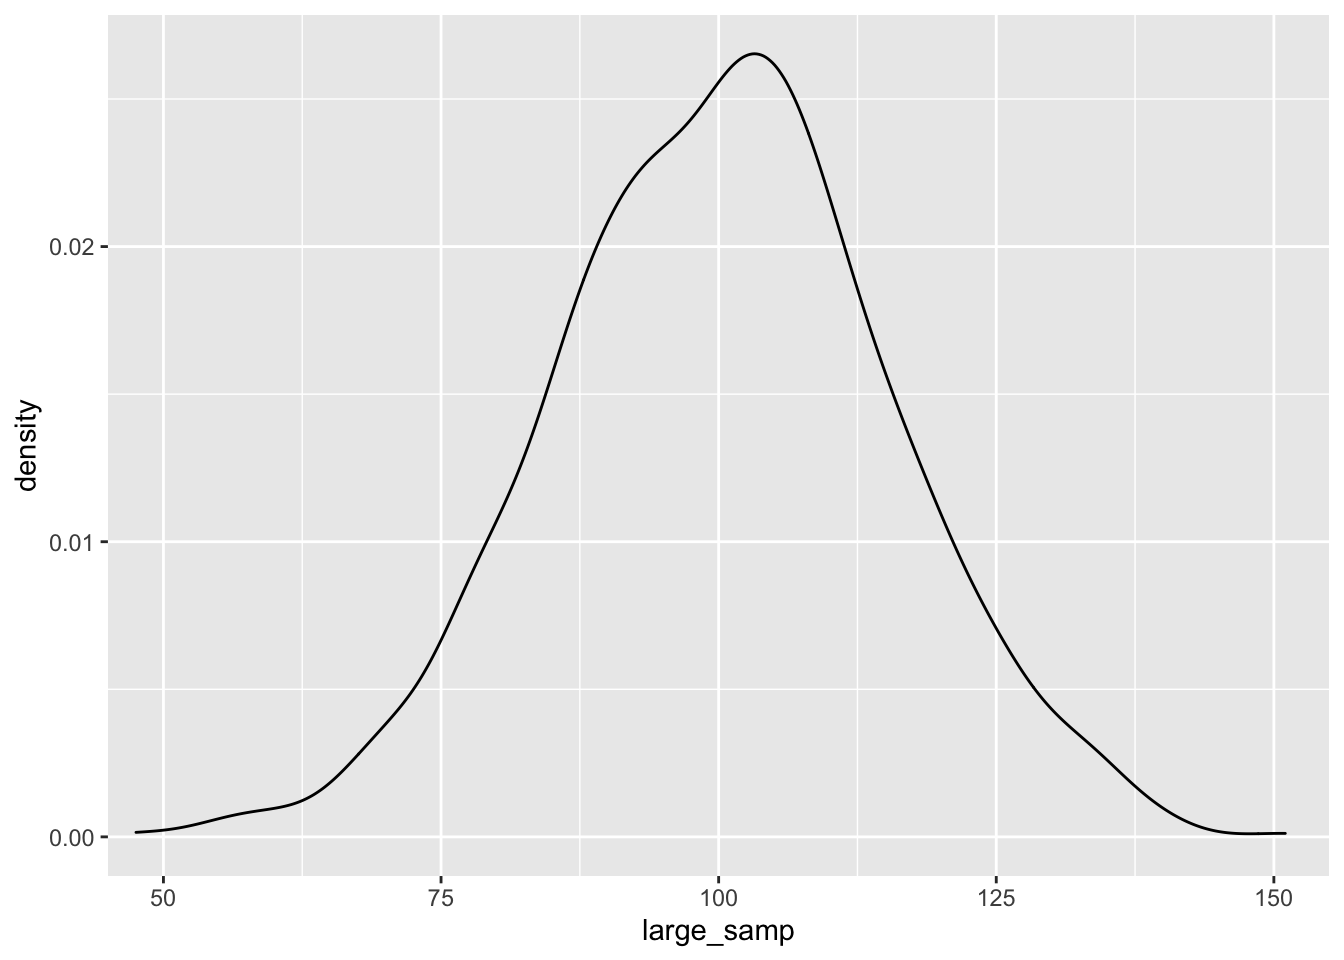
\includegraphics{r4psych_files/figure-latex/8_norm_sample_sizes-2.pdf}

As before, the data seem to fit the population distribution better when we have larger sample sizes. Let's change the standard deviation to see how variance in our samples influences the distribution of effects. Here, we'll just focus on the larger sample size:

\begin{Shaded}
\begin{Highlighting}[]
\FunctionTok{set.seed}\NormalTok{(}\DecValTok{5}\NormalTok{)}
\NormalTok{large\_sd\_samp }\OtherTok{\textless{}{-}} \FunctionTok{rnorm}\NormalTok{(}\AttributeTok{n =} \DecValTok{1000}\NormalTok{, }\AttributeTok{mean =} \DecValTok{100}\NormalTok{, }\AttributeTok{sd =} \DecValTok{15}\NormalTok{)}
\NormalTok{small\_sd\_samp }\OtherTok{\textless{}{-}} \FunctionTok{rnorm}\NormalTok{(}\AttributeTok{n =} \DecValTok{1000}\NormalTok{, }\AttributeTok{mean =} \DecValTok{100}\NormalTok{, }\AttributeTok{sd =} \FloatTok{1.5}\NormalTok{)}

\FunctionTok{ggplot}\NormalTok{() }\SpecialCharTok{+} \FunctionTok{geom\_density}\NormalTok{(}\FunctionTok{aes}\NormalTok{(large\_sd\_samp)) }\SpecialCharTok{+} \FunctionTok{coord\_cartesian}\NormalTok{(}\AttributeTok{x =} \FunctionTok{c}\NormalTok{(}\DecValTok{50}\NormalTok{, }\DecValTok{150}\NormalTok{))}
\end{Highlighting}
\end{Shaded}

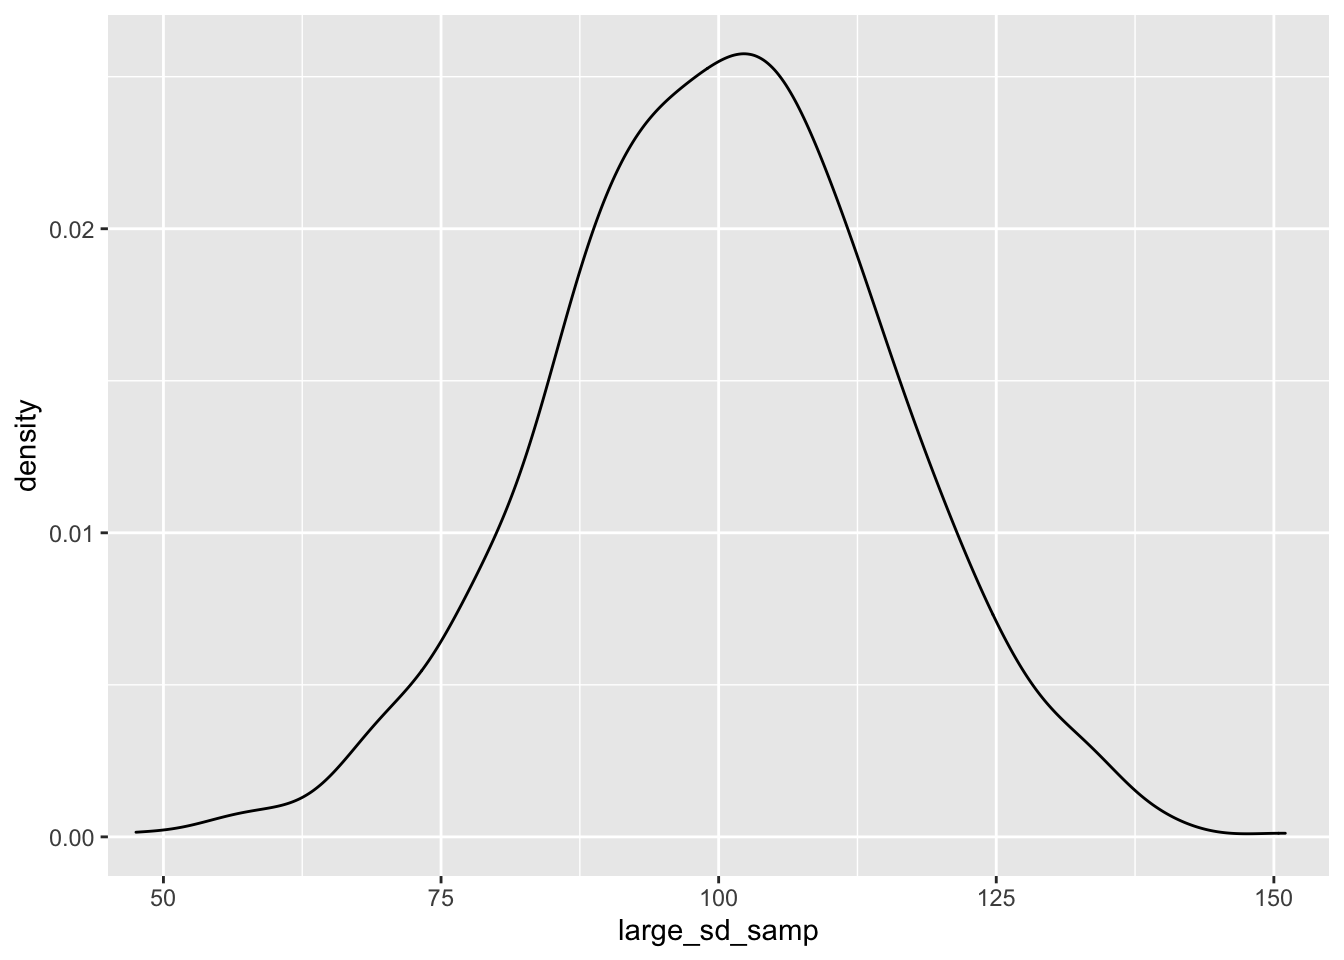
\includegraphics{r4psych_files/figure-latex/8_norm_standard_deviation-1.pdf}

\begin{Shaded}
\begin{Highlighting}[]
\FunctionTok{ggplot}\NormalTok{() }\SpecialCharTok{+} \FunctionTok{geom\_density}\NormalTok{(}\FunctionTok{aes}\NormalTok{(small\_sd\_samp)) }\SpecialCharTok{+} \FunctionTok{coord\_cartesian}\NormalTok{(}\AttributeTok{x =} \FunctionTok{c}\NormalTok{(}\DecValTok{50}\NormalTok{, }\DecValTok{150}\NormalTok{))}
\end{Highlighting}
\end{Shaded}

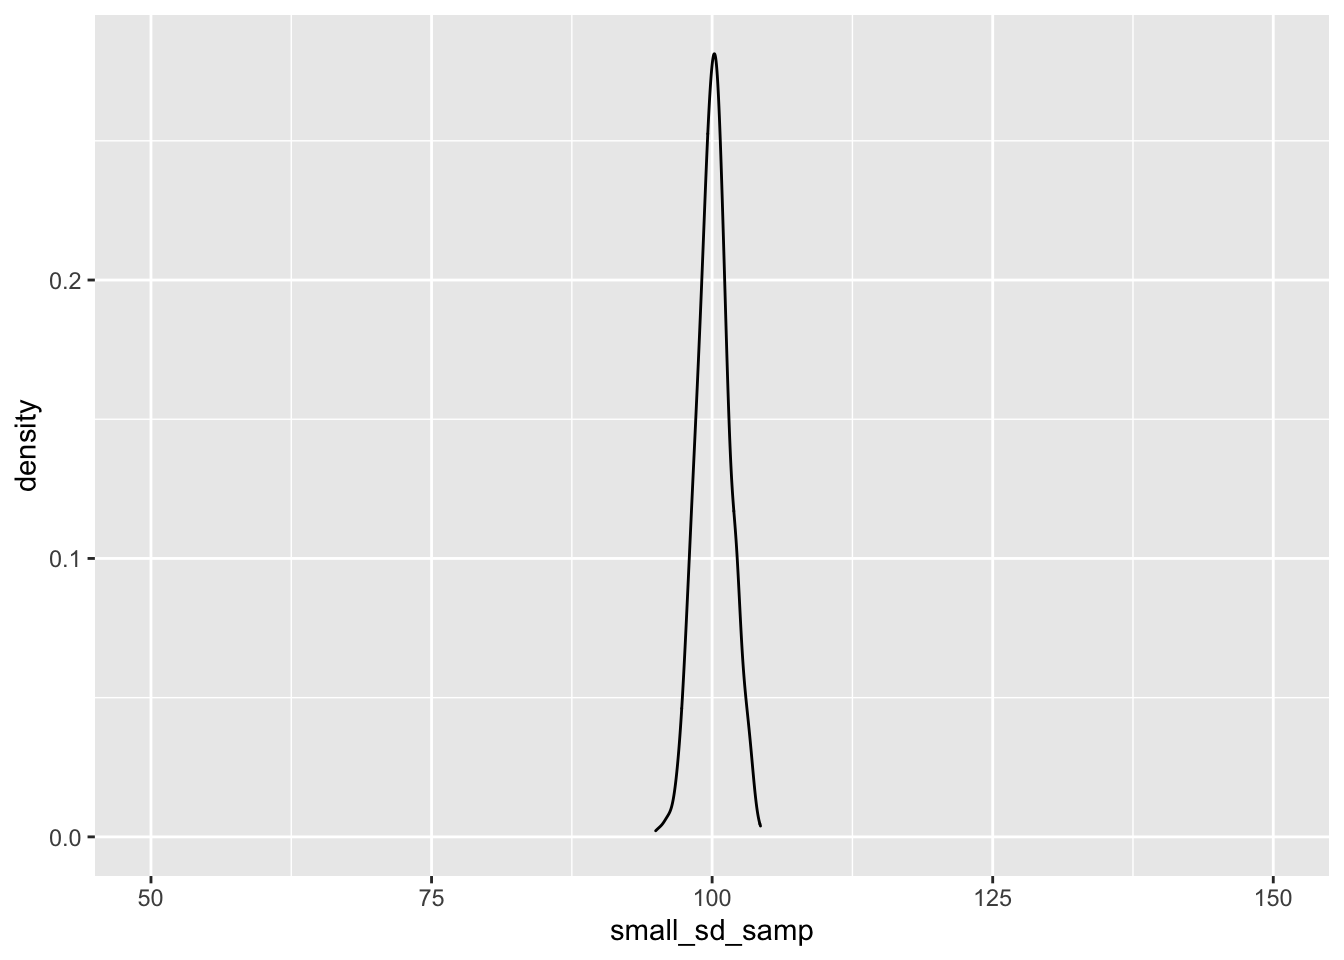
\includegraphics{r4psych_files/figure-latex/8_norm_standard_deviation-2.pdf}

As you can see, as we sample from a population with a smaller standard deviation, our samples will be closer to the mean score. This has important implications for our statistical tests; the larger the standard deviation within our samples, the more samples we'll need to detect an effect.

\hypertarget{the-binomial-distribution}{%
\subsection{The Binomial Distribution}\label{the-binomial-distribution}}

Next, we'll look at sampling from a binomial distribution. We might use this to generate data on a binomial scale, such as the probability of a success/failure in a task (e.g.~did they get the question right or not?). We sample from a binomial distribution using the \texttt{rbinom()} function.

This function takes 3 arguments: \texttt{n}, the number of observations we'd like to see; \texttt{size}, the number of trials within an observation; and \texttt{prob} the probability of a success (1) (vs.~failure, 0) on each trial.

Below, we'll get 10 observations, of 1 trial each, with a success rate of 50\% on each trial.

\begin{Shaded}
\begin{Highlighting}[]
\FunctionTok{set.seed}\NormalTok{(}\DecValTok{1000}\NormalTok{)}
\FunctionTok{rbinom}\NormalTok{(}\AttributeTok{n =} \DecValTok{10}\NormalTok{, }\AttributeTok{size =} \DecValTok{1}\NormalTok{, }\AttributeTok{prob =} \FloatTok{0.5}\NormalTok{)}
\end{Highlighting}
\end{Shaded}

\begin{verbatim}
##  [1] 0 1 0 1 1 0 1 1 0 0
\end{verbatim}

As you can see, our sampling produced 5 successes (1) and 5 failures (0). What if we want to make each observation the number of successes in 20 trials. Let's change the size argument to 20.

\begin{Shaded}
\begin{Highlighting}[]
\FunctionTok{set.seed}\NormalTok{(}\DecValTok{1000}\NormalTok{)}
\FunctionTok{rbinom}\NormalTok{(}\AttributeTok{n =} \DecValTok{10}\NormalTok{, }\AttributeTok{size =} \DecValTok{20}\NormalTok{, }\AttributeTok{prob =} \FloatTok{0.5}\NormalTok{)}
\end{Highlighting}
\end{Shaded}

\begin{verbatim}
##  [1]  9 12  7 11 10  7 11 10  8  9
\end{verbatim}

Now each trial roughly follows a 50\% success rate as before, but each observation is out of 20 trials. We can convert these to proportions by simply dividing the whole thing by the same value as our size argument.

\begin{Shaded}
\begin{Highlighting}[]
\FunctionTok{set.seed}\NormalTok{(}\DecValTok{1000}\NormalTok{)}
\FunctionTok{rbinom}\NormalTok{(}\AttributeTok{n =} \DecValTok{10}\NormalTok{, }\AttributeTok{size =} \DecValTok{20}\NormalTok{, }\AttributeTok{prob =} \FloatTok{0.5}\NormalTok{) }\SpecialCharTok{/} \DecValTok{20}
\end{Highlighting}
\end{Shaded}

\begin{verbatim}
##  [1] 0.45 0.60 0.35 0.55 0.50 0.35 0.55 0.50 0.40 0.45
\end{verbatim}

Did you notice the repetition of 20 in our code? We'll save some repetition for the value of 20 by defining the number of trials in a separate object, and passing the name of this object to our argument. This should get you used to using objects as holders for values as a precursor to writing your own functions!

\begin{Shaded}
\begin{Highlighting}[]
\CommentTok{\# define number of trials}
\NormalTok{n\_trials }\OtherTok{\textless{}{-}} \DecValTok{20}

\FunctionTok{set.seed}\NormalTok{(}\DecValTok{1000}\NormalTok{)}
\FunctionTok{rbinom}\NormalTok{(}\AttributeTok{n =} \DecValTok{10}\NormalTok{, }\AttributeTok{size =}\NormalTok{ n\_trials, }\AttributeTok{prob =} \FloatTok{0.5}\NormalTok{) }\SpecialCharTok{/}\NormalTok{ n\_trials}
\end{Highlighting}
\end{Shaded}

\begin{verbatim}
##  [1] 0.45 0.60 0.35 0.55 0.50 0.35 0.55 0.50 0.40 0.45
\end{verbatim}

Also, I think our code is a bit more readable now that we know what the 20 represents!

Can you guess what the mean of a 1000 samples might look like? What about the distribution of these? Try calculating the mean of 1000 samples of 20 trials with a probability of 0.5 and plot this out using a histrogram.

\hypertarget{flexible-sampling}{%
\subsection{Flexible Sampling}\label{flexible-sampling}}

Finally, we can also randomly sample discrete variables with pre-defined probabilities. Nicely, we can use the same function to do this for strings of character or for integers. To do this, we use the \texttt{sample()} function. This is useful for creating dummy data sets where we might want to randomly sample names for participants, or outcomes with a bias on our draws.

We can simply define what to sample from with the \texttt{x} argument. If this is an integer, R will sample from any positive integer up to and including this limit. As before we can ask for any number of samples with the \texttt{size} argument.

Finally, we can specify if we want to replace these numbers with the \texttt{replace} argument. If we set this to true, R puts any drawn numbers back in the bag before picking them out again. If we set this to FALSE, R will not put the numbers back in the bag before drawing again, so we can't redraw the same number.

\begin{Shaded}
\begin{Highlighting}[]
\FunctionTok{set.seed}\NormalTok{(}\DecValTok{1000}\NormalTok{)}
\FunctionTok{sample}\NormalTok{(}\AttributeTok{x =} \DecValTok{10}\NormalTok{, }\AttributeTok{size =} \DecValTok{10}\NormalTok{, }\AttributeTok{replace =} \ConstantTok{TRUE}\NormalTok{)}
\end{Highlighting}
\end{Shaded}

\begin{verbatim}
##  [1] 4 6 3 8 3 2 6 6 6 1
\end{verbatim}

Did you notice how we got 3 twice? Let's change the \texttt{replace} argument to \texttt{FALSE} to see what happens.

\begin{Shaded}
\begin{Highlighting}[]
\FunctionTok{set.seed}\NormalTok{(}\DecValTok{1000}\NormalTok{)}
\FunctionTok{sample}\NormalTok{(}\AttributeTok{x =} \DecValTok{10}\NormalTok{, }\AttributeTok{size =} \DecValTok{10}\NormalTok{, }\AttributeTok{replace =} \ConstantTok{FALSE}\NormalTok{)}
\end{Highlighting}
\end{Shaded}

\begin{verbatim}
##  [1]  4  6  3  5  8  7  2 10  9  1
\end{verbatim}

Now we only get unique numbers. If we ask to draw more numbers than we have unique values, this will fail.

\begin{Shaded}
\begin{Highlighting}[]
\FunctionTok{set.seed}\NormalTok{(}\DecValTok{1000}\NormalTok{)}
\FunctionTok{sample}\NormalTok{(}\AttributeTok{x =} \DecValTok{10}\NormalTok{, }\AttributeTok{size =} \DecValTok{11}\NormalTok{, }\AttributeTok{replace =} \ConstantTok{FALSE}\NormalTok{)}
\end{Highlighting}
\end{Shaded}

We can also sample from characters, such as when we might want to create some data for the names of participants.

\begin{Shaded}
\begin{Highlighting}[]
\FunctionTok{set.seed}\NormalTok{(}\DecValTok{1000}\NormalTok{)}
\NormalTok{names }\OtherTok{\textless{}{-}} \FunctionTok{c}\NormalTok{(}\StringTok{"Glenn"}\NormalTok{, }\StringTok{"Nik"}\NormalTok{, }\StringTok{"Vera"}\NormalTok{, }\StringTok{"Neil"}\NormalTok{)}
\FunctionTok{sample}\NormalTok{(}\AttributeTok{x =}\NormalTok{ names, }\AttributeTok{size =} \DecValTok{2}\NormalTok{, }\AttributeTok{replace =} \ConstantTok{TRUE}\NormalTok{)}
\end{Highlighting}
\end{Shaded}

\begin{verbatim}
## [1] "Neil" "Neil"
\end{verbatim}

We can also set some pre-defined probabilities for the things we'll sample from. Let's say the probability of selecting ``Glenn'' is most likely in 10 draws.

\begin{Shaded}
\begin{Highlighting}[]
\FunctionTok{set.seed}\NormalTok{(}\DecValTok{1000}\NormalTok{)}
\NormalTok{names }\OtherTok{\textless{}{-}} \FunctionTok{c}\NormalTok{(}\StringTok{"Glenn"}\NormalTok{, }\StringTok{"Nik"}\NormalTok{, }\StringTok{"Vera"}\NormalTok{, }\StringTok{"Neil"}\NormalTok{)}
\FunctionTok{sample}\NormalTok{(}\AttributeTok{x =}\NormalTok{ names, }\AttributeTok{size =} \DecValTok{10}\NormalTok{, }\AttributeTok{replace =} \ConstantTok{TRUE}\NormalTok{, }\AttributeTok{prob =} \FunctionTok{c}\NormalTok{(}\FloatTok{0.7}\NormalTok{, }\FloatTok{0.1}\NormalTok{, }\FloatTok{0.1}\NormalTok{, }\FloatTok{0.1}\NormalTok{))}
\end{Highlighting}
\end{Shaded}

\begin{verbatim}
##  [1] "Glenn" "Vera"  "Glenn" "Glenn" "Glenn" "Glenn" "Vera"  "Glenn" "Glenn"
## [10] "Glenn"
\end{verbatim}

As you can see, Glenn gets drawn most often because this has the highest probability to be drawn (i.e.~the first thing in \texttt{x} is related to the first probability in \texttt{prob}).

This sampling procedure is very flexible for simulating data if we have some idea about the probabilities for things to be sampled. Let's look at an example where sampling like this is useful.

\hypertarget{sampling-for-inference}{%
\section{Sampling for Inference}\label{sampling-for-inference}}

Imagine we're studying a person who claims to be a psychic. We decide to test their claim by getting them to take part in an experiment. In this experiment, we have 10 cards each with 1 of 5 symbols on the back. The psychic says that they can guess, above chance, which symbol is on the back of the card.

Let's simulate their data for 10 attempts.

\begin{Shaded}
\begin{Highlighting}[]
\CommentTok{\# sample the true values of the cards}
\FunctionTok{set.seed}\NormalTok{(}\DecValTok{13}\NormalTok{)}
\NormalTok{psychic\_outcome }\OtherTok{\textless{}{-}} \FunctionTok{rbinom}\NormalTok{(}\AttributeTok{n =} \DecValTok{1}\NormalTok{, }\AttributeTok{size =} \DecValTok{10}\NormalTok{, }\AttributeTok{prob =} \FloatTok{0.2}\NormalTok{)}

\CommentTok{\# see the true values}
\NormalTok{psychic\_outcome}
\end{Highlighting}
\end{Shaded}

\begin{verbatim}
## [1] 3
\end{verbatim}

The psychic guessed 3 cards correctly out of 10. However, we know that on each trial, the probability of a success is only 20\% (i.e.~1 in 5). Was the psychic telling the truth, or should we have reason to doubt their claim?

\begin{Shaded}
\begin{Highlighting}[]
\FunctionTok{binom.test}\NormalTok{(}\AttributeTok{x =}\NormalTok{ psychic\_outcome, }\AttributeTok{n =} \DecValTok{10}\NormalTok{, }\AttributeTok{p =} \FloatTok{0.2}\NormalTok{)}
\end{Highlighting}
\end{Shaded}

\begin{verbatim}
## 
##  Exact binomial test
## 
## data:  psychic_outcome and 10
## number of successes = 3, number of trials = 10, p-value = 0.4296
## alternative hypothesis: true probability of success is not equal to 0.2
## 95 percent confidence interval:
##  0.06673951 0.65245285
## sample estimates:
## probability of success 
##                    0.3
\end{verbatim}

So, it seems that although they performed above chance, the sample size is too small to consider this difference between the observed and expected probability of success to be meaningful.

What if we change it so the psychic got it right 30 times in 100 chances? We'll simply multiply the number of successes and observations by 10 and test for a significant difference between the observed and expected probability.

\begin{Shaded}
\begin{Highlighting}[]
\FunctionTok{binom.test}\NormalTok{(}\AttributeTok{x =}\NormalTok{ psychic\_outcome }\SpecialCharTok{*} \DecValTok{10}\NormalTok{, }\AttributeTok{n =} \DecValTok{10} \SpecialCharTok{*} \DecValTok{10}\NormalTok{, }\AttributeTok{p =} \FloatTok{0.2}\NormalTok{)}
\end{Highlighting}
\end{Shaded}

\begin{verbatim}
## 
##  Exact binomial test
## 
## data:  psychic_outcome * 10 and 10 * 10
## number of successes = 30, number of trials = 100, p-value = 0.01695
## alternative hypothesis: true probability of success is not equal to 0.2
## 95 percent confidence interval:
##  0.2124064 0.3998147
## sample estimates:
## probability of success 
##                    0.3
\end{verbatim}

Now we have a significant effect showing indicating that we should reject the null hypothesis. But do any of you really believe that the psychic is truly psychic? Remember that we used the binomial sampling procedure to come up with these scores in the first place, so we know that the true probability of a success on each trial is 0.2, or 20\%, which is chance.

Let's change our sampling procedure into a function so we can better explore whether or not we should trust the outcome of this one study. Before we do so, we'll see how functions work, and why they are useful in our work.

\hypertarget{understanding-p-values-and-type-i-errors}{%
\subsection{Understanding p-values and Type-I Errors}\label{understanding-p-values-and-type-i-errors}}

User defined functions in R take the form of:

\begin{Shaded}
\begin{Highlighting}[]
\NormalTok{function\_name }\OtherTok{\textless{}{-}} \ControlFlowTok{function}\NormalTok{(parameters\_to\_vary) \{}
\NormalTok{  things\_for\_the\_function\_to\_do}
\NormalTok{\}}
\end{Highlighting}
\end{Shaded}

We first have to specify a name for our function. Often, it's best to use verb-like naming here, as your functions are things you want to do to something (e.g.~calculate descriptive statitics etc.). You then assign to this name how the function works. Within the function call in parentheses, you can define different parameters of your function that you'd like to vary. This simply makes your function flexible to doing things to data with different inputs. Finally, within the body of the function, \texttt{\{here\ is\ the\ body\}}, we define things to do to your parameters that are passed to the function. The last thing that you type in your function is what your function returns to you when you run it (i.e.~what you will see when you run the function).

Let's transform our sampling and testing procedure into a function. I've commented this code so you understand how it works.

\begin{Shaded}
\begin{Highlighting}[]
\CommentTok{\# define function name and parameters to vary}
\NormalTok{simulate\_psychic\_test }\OtherTok{\textless{}{-}} \ControlFlowTok{function}\NormalTok{(n\_trials, prob\_success) \{}
  
  \CommentTok{\# sample binomial data (successs or not) for varying trials and probabilities }
\NormalTok{  psychic\_outcome }\OtherTok{\textless{}{-}} \FunctionTok{rbinom}\NormalTok{(}\AttributeTok{n =} \DecValTok{1}\NormalTok{, }\AttributeTok{size =}\NormalTok{ n\_trials, }\AttributeTok{prob =}\NormalTok{ prob\_success)}
  
  \CommentTok{\# run a binomial test on the sampled data against your proability}
\NormalTok{  test }\OtherTok{\textless{}{-}} \FunctionTok{binom.test}\NormalTok{(}\AttributeTok{x =}\NormalTok{ psychic\_outcome, }\AttributeTok{n =}\NormalTok{ n\_trials, }\AttributeTok{p =}\NormalTok{ prob\_success)}
  
  \CommentTok{\# retrieve the p{-}value, this is what is returned in our function}
\NormalTok{  test}\SpecialCharTok{$}\NormalTok{p.value}
\NormalTok{\}}
\end{Highlighting}
\end{Shaded}

Congratulations, you've just made your first user-defined function in R! Here, we've defined a function that will take a number of trials and a probability of success on each trial. It will then sample some data under those parameters, before testing it against the probability of success. Finally, it will extract the \emph{p}-value from that test and return it to you. Let's see this in action.

Run and rerun the code below several times to see what happens. What do the \emph{p}-values look like? Remember, a value below 0.05 is typical in psychology for the cut-off point where we'll reject the null hypothesis of no difference between the observed and predicted probabilities of success.

\begin{Shaded}
\begin{Highlighting}[]
\FunctionTok{simulate\_psychic\_test}\NormalTok{(}\AttributeTok{n\_trials =} \DecValTok{100}\NormalTok{, }\AttributeTok{prob\_success =} \FloatTok{0.2}\NormalTok{)}
\end{Highlighting}
\end{Shaded}

\begin{verbatim}
## [1] 0.5322562
\end{verbatim}

Ok, so you've seen how these \emph{p}-values shift even when we know there's no true effect. Let's simulate the experiment 100 times to see what happens to the distribution of the \emph{p}-values.

Nicely, R has a \texttt{replicate()} function, which replicates whatever we ask it to do by a pre-defined number. This replicate function takes \texttt{n} as an argument, which is the number of replication to carry out, plus whatever you want to replicate.

Can you predict what will happen?

\begin{Shaded}
\begin{Highlighting}[]
\NormalTok{simulations }\OtherTok{\textless{}{-}} \FunctionTok{replicate}\NormalTok{(}\AttributeTok{n =} \DecValTok{100}\NormalTok{, }
                         \FunctionTok{simulate\_psychic\_test}\NormalTok{(}\AttributeTok{n\_trials =} \DecValTok{100}\NormalTok{, }
                                               \AttributeTok{prob\_success =} \FloatTok{0.2}
\NormalTok{                                               )}
\NormalTok{                         )}
\end{Highlighting}
\end{Shaded}

\begin{Shaded}
\begin{Highlighting}[]
\FunctionTok{ggplot}\NormalTok{() }\SpecialCharTok{+} 
  \FunctionTok{geom\_histogram}\NormalTok{(}\AttributeTok{mapping =} \FunctionTok{aes}\NormalTok{(simulations),}
                 \AttributeTok{binwidth =} \FloatTok{0.05}\NormalTok{,}
                 \AttributeTok{boundary =} \DecValTok{0}\NormalTok{,}
                 \AttributeTok{fill =} \StringTok{"white"}\NormalTok{,}
                 \AttributeTok{colour =} \StringTok{"black"}\NormalTok{) }\SpecialCharTok{+}
  \FunctionTok{scale\_x\_continuous}\NormalTok{(}\AttributeTok{limits =} \FunctionTok{c}\NormalTok{(}\DecValTok{0}\NormalTok{, }\DecValTok{1}\NormalTok{), }
                     \AttributeTok{breaks =} \FunctionTok{seq}\NormalTok{(}\AttributeTok{from =} \DecValTok{0}\NormalTok{, }\AttributeTok{to =} \DecValTok{1}\NormalTok{, }\AttributeTok{by =} \FloatTok{0.05}\NormalTok{)}
\NormalTok{                     ) }\SpecialCharTok{+}
  \FunctionTok{geom\_vline}\NormalTok{(}\AttributeTok{xintercept =} \FloatTok{0.05}\NormalTok{, }\AttributeTok{linetype =} \DecValTok{2}\NormalTok{, }\AttributeTok{colour =} \StringTok{"red"}\NormalTok{) }\SpecialCharTok{+}
  \FunctionTok{labs}\NormalTok{(}\AttributeTok{x =} \StringTok{"p{-}value"}\NormalTok{) }\SpecialCharTok{+}
  \FunctionTok{theme}\NormalTok{(}\AttributeTok{axis.text.x =} \FunctionTok{element\_text}\NormalTok{(}\AttributeTok{size=}\DecValTok{8}\NormalTok{))}
\end{Highlighting}
\end{Shaded}

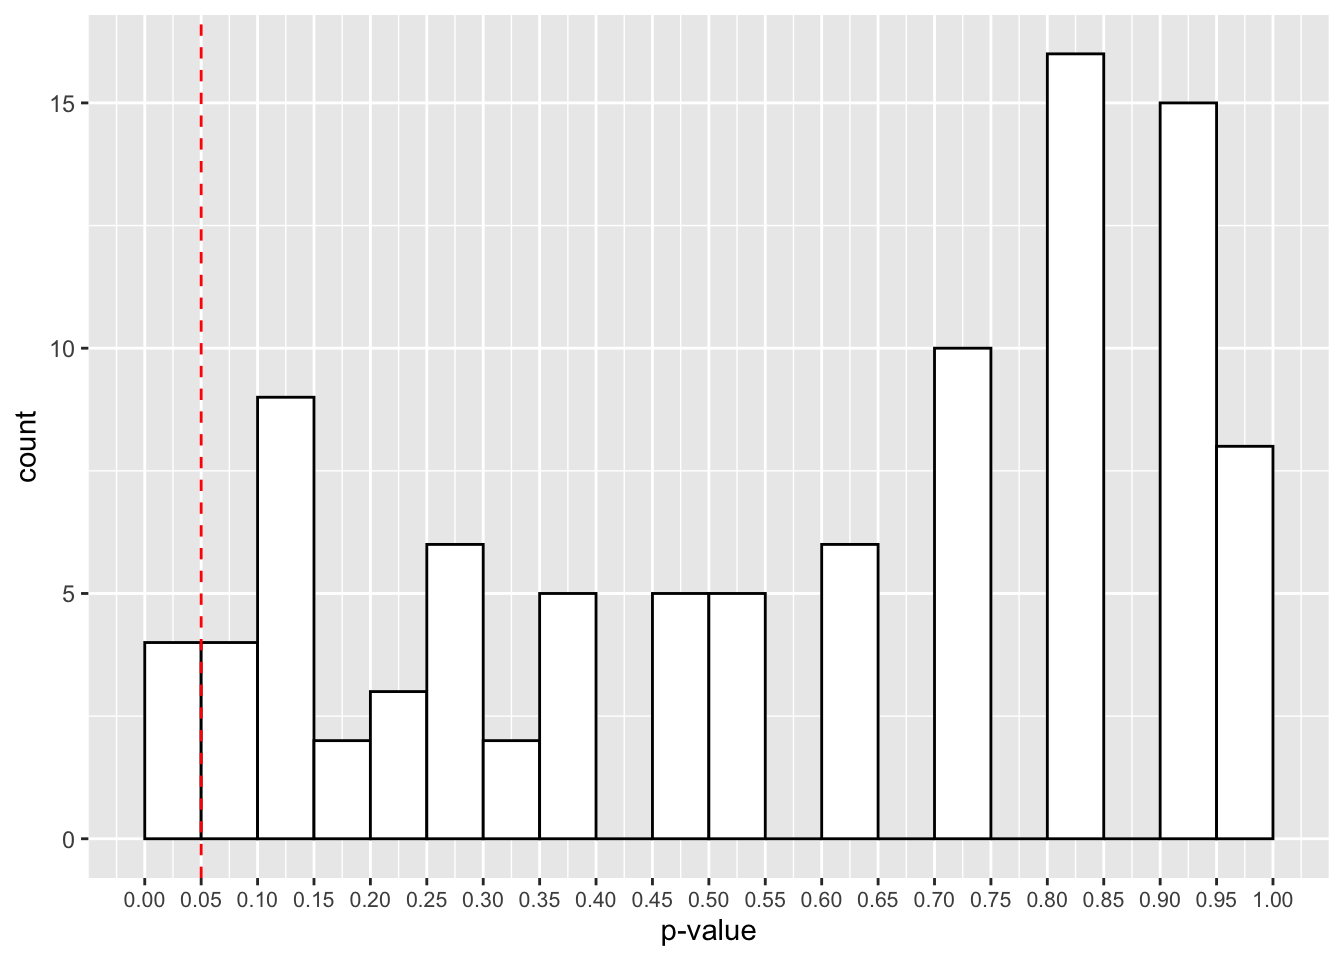
\includegraphics{r4psych_files/figure-latex/8_simulate_function_plot-1.pdf}

The red cut-off line shows the number of values that fall below our 0.05 cut-off point for our \emph{p}-values. That looks like roughly 3 in 100 samples, or 3\% of our simulated studies.

Try increasing the number of replications for the experiment to see how the \emph{p}-values change. How does it look with 10,000 simulated studies?

\begin{Shaded}
\begin{Highlighting}[]
\NormalTok{simulations }\OtherTok{\textless{}{-}} \FunctionTok{replicate}\NormalTok{(}\AttributeTok{n =} \DecValTok{10000}\NormalTok{, }
                         \FunctionTok{simulate\_psychic\_test}\NormalTok{(}\AttributeTok{n\_trials =} \DecValTok{100}\NormalTok{, }
                                               \AttributeTok{prob\_success =} \FloatTok{0.2}
\NormalTok{                                               )}
\NormalTok{                         )}
\end{Highlighting}
\end{Shaded}

\begin{Shaded}
\begin{Highlighting}[]
\FunctionTok{ggplot}\NormalTok{() }\SpecialCharTok{+} 
  \FunctionTok{geom\_histogram}\NormalTok{(}\FunctionTok{aes}\NormalTok{(simulations),}
                 \AttributeTok{binwidth =} \FloatTok{0.05}\NormalTok{,}
                 \AttributeTok{boundary =} \DecValTok{0}\NormalTok{,}
                 \AttributeTok{fill =} \StringTok{"white"}\NormalTok{,}
                 \AttributeTok{colour =} \StringTok{"black"}\NormalTok{) }\SpecialCharTok{+}
  \FunctionTok{scale\_x\_continuous}\NormalTok{(}\AttributeTok{limits =} \FunctionTok{c}\NormalTok{(}\DecValTok{0}\NormalTok{, }\DecValTok{1}\NormalTok{), }
                     \AttributeTok{breaks =} \FunctionTok{seq}\NormalTok{(}\AttributeTok{from =} \DecValTok{0}\NormalTok{, }\AttributeTok{to =} \DecValTok{1}\NormalTok{, }\AttributeTok{by =} \FloatTok{0.05}\NormalTok{)}
\NormalTok{                     ) }\SpecialCharTok{+}
  \FunctionTok{geom\_vline}\NormalTok{(}\AttributeTok{xintercept =} \FloatTok{0.05}\NormalTok{, }\AttributeTok{linetype =} \DecValTok{2}\NormalTok{, }\AttributeTok{colour =} \StringTok{"red"}\NormalTok{) }\SpecialCharTok{+}
  \FunctionTok{labs}\NormalTok{(}\AttributeTok{x =} \StringTok{"p{-}value"}\NormalTok{) }\SpecialCharTok{+}
  \FunctionTok{theme}\NormalTok{(}\AttributeTok{axis.text.x =} \FunctionTok{element\_text}\NormalTok{(}\AttributeTok{size=}\DecValTok{8}\NormalTok{))}
\end{Highlighting}
\end{Shaded}

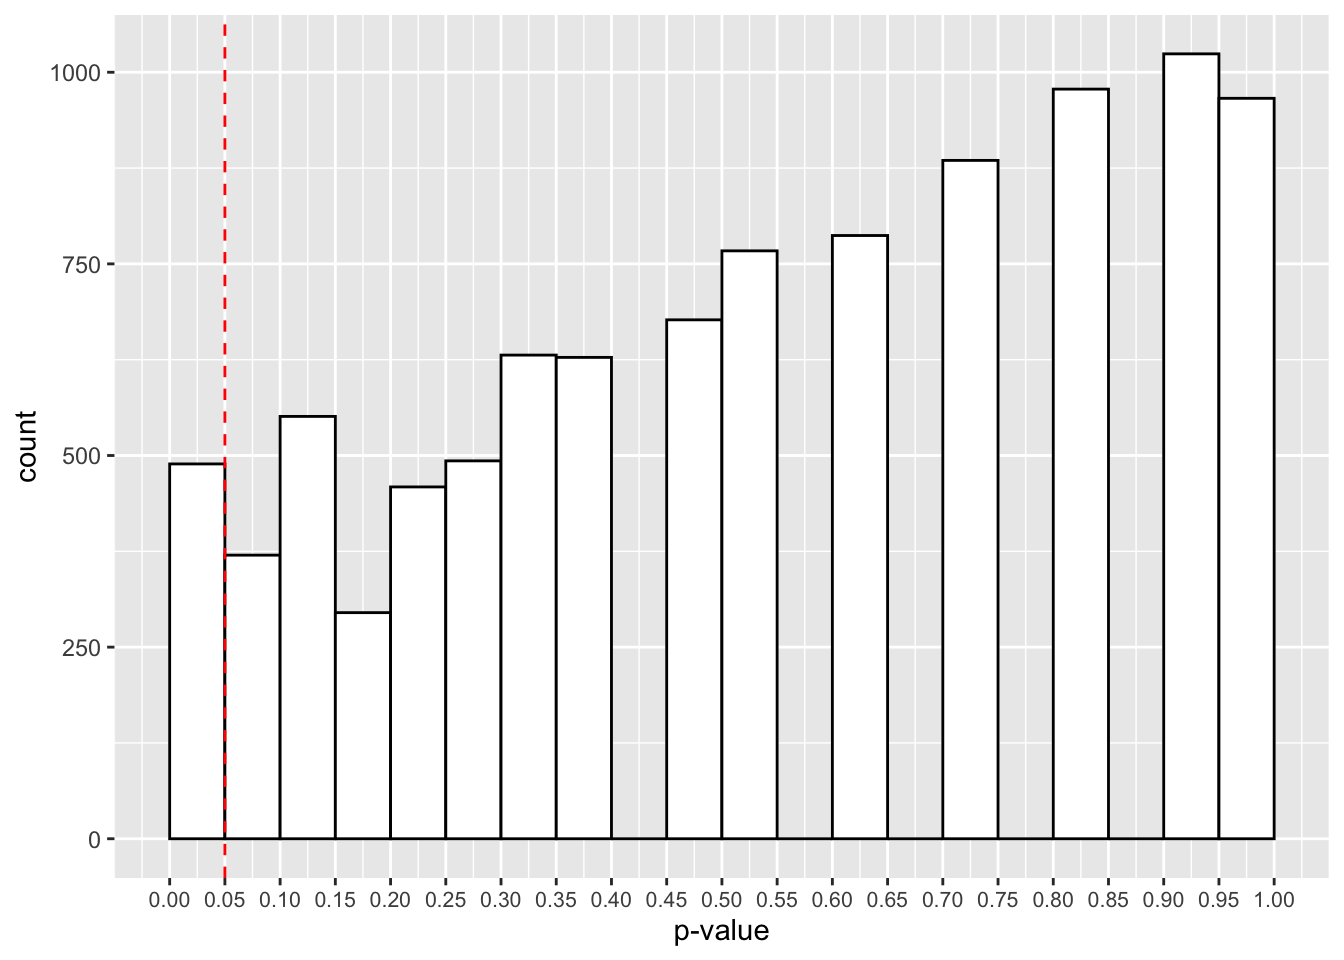
\includegraphics{r4psych_files/figure-latex/8_simulate_function_replications_plot-1.pdf}

Here we have roughly 500 studies showing \emph{p}-values below 0.05. Thats 5\% of the 10,000 studies. Is that surprising? Even when there's no effect in the population, with repeated sampling we're bound to find some cases where we have \emph{p}-values below 0.05. That's why replications are so important for our research!

This false-positive rate is the type-I error rate of our study, and is determined by our \emph{p}-value. This determines the amount of time we will incorrectly reject the null hypothesis in the long run (i.e.~if we run several studies over time).

\hypertarget{understanding-power-and-type-ii-errors}{%
\subsection{Understanding Power and Type-II Errors}\label{understanding-power-and-type-ii-errors}}

What if we change our function so that we can give the psychic a different probability to the true probability of a success?

\begin{Shaded}
\begin{Highlighting}[]
\CommentTok{\# define function name and parameters to vary}
\NormalTok{simulate\_psychic\_test }\OtherTok{\textless{}{-}} \ControlFlowTok{function}\NormalTok{(n\_trials, prob\_success, psychic\_success) \{}
  
  \CommentTok{\# sample binomial data (successs or not) for varying trials and probabilities }
\NormalTok{  psychic\_outcome }\OtherTok{\textless{}{-}} \FunctionTok{rbinom}\NormalTok{(}\AttributeTok{n =} \DecValTok{1}\NormalTok{, }\AttributeTok{size =}\NormalTok{ n\_trials, }\AttributeTok{prob =}\NormalTok{ psychic\_success)}
  
  \CommentTok{\# run a binomial test on the sampled data against your proability}
\NormalTok{  test }\OtherTok{\textless{}{-}} \FunctionTok{binom.test}\NormalTok{(}\AttributeTok{x =}\NormalTok{ psychic\_outcome, }\AttributeTok{n =}\NormalTok{ n\_trials, }\AttributeTok{p =}\NormalTok{ prob\_success)}
  
  \CommentTok{\# retrieve the p{-}value, this is what is returned in our function}
\NormalTok{  test}\SpecialCharTok{$}\NormalTok{p.value}
\NormalTok{\}}
\end{Highlighting}
\end{Shaded}

\begin{Shaded}
\begin{Highlighting}[]
\NormalTok{true\_effect\_simulations }\OtherTok{\textless{}{-}} \FunctionTok{replicate}\NormalTok{(}\AttributeTok{n =} \DecValTok{1000}\NormalTok{, }
                         \FunctionTok{simulate\_psychic\_test}\NormalTok{(}\AttributeTok{n\_trials =} \DecValTok{100}\NormalTok{, }
                                               \AttributeTok{prob\_success =} \FloatTok{0.2}\NormalTok{,}
                                               \AttributeTok{psychic\_success =} \FloatTok{0.25}
\NormalTok{                                               )}
\NormalTok{                         )}
\end{Highlighting}
\end{Shaded}

\begin{Shaded}
\begin{Highlighting}[]
\FunctionTok{ggplot}\NormalTok{() }\SpecialCharTok{+} 
  \FunctionTok{geom\_histogram}\NormalTok{(}\FunctionTok{aes}\NormalTok{(true\_effect\_simulations),}
                 \AttributeTok{binwidth =} \FloatTok{0.05}\NormalTok{,}
                 \AttributeTok{boundary =} \DecValTok{0}\NormalTok{,}
                 \AttributeTok{fill =} \StringTok{"white"}\NormalTok{,}
                 \AttributeTok{colour =} \StringTok{"black"}\NormalTok{) }\SpecialCharTok{+}
  \FunctionTok{scale\_x\_continuous}\NormalTok{(}\AttributeTok{limits =} \FunctionTok{c}\NormalTok{(}\DecValTok{0}\NormalTok{, }\DecValTok{1}\NormalTok{), }
                     \AttributeTok{breaks =} \FunctionTok{seq}\NormalTok{(}\AttributeTok{from =} \DecValTok{0}\NormalTok{, }\AttributeTok{to =} \DecValTok{1}\NormalTok{, }\AttributeTok{by =} \FloatTok{0.05}\NormalTok{)}
\NormalTok{                     ) }\SpecialCharTok{+}
  \FunctionTok{geom\_vline}\NormalTok{(}\AttributeTok{xintercept =} \FloatTok{0.05}\NormalTok{, }\AttributeTok{linetype =} \DecValTok{2}\NormalTok{, }\AttributeTok{colour =} \StringTok{"red"}\NormalTok{) }\SpecialCharTok{+}
  \FunctionTok{labs}\NormalTok{(}\AttributeTok{x =} \StringTok{"p{-}value"}\NormalTok{) }\SpecialCharTok{+}
  \FunctionTok{theme}\NormalTok{(}\AttributeTok{axis.text.x =} \FunctionTok{element\_text}\NormalTok{(}\AttributeTok{size=}\DecValTok{8}\NormalTok{))}
\end{Highlighting}
\end{Shaded}

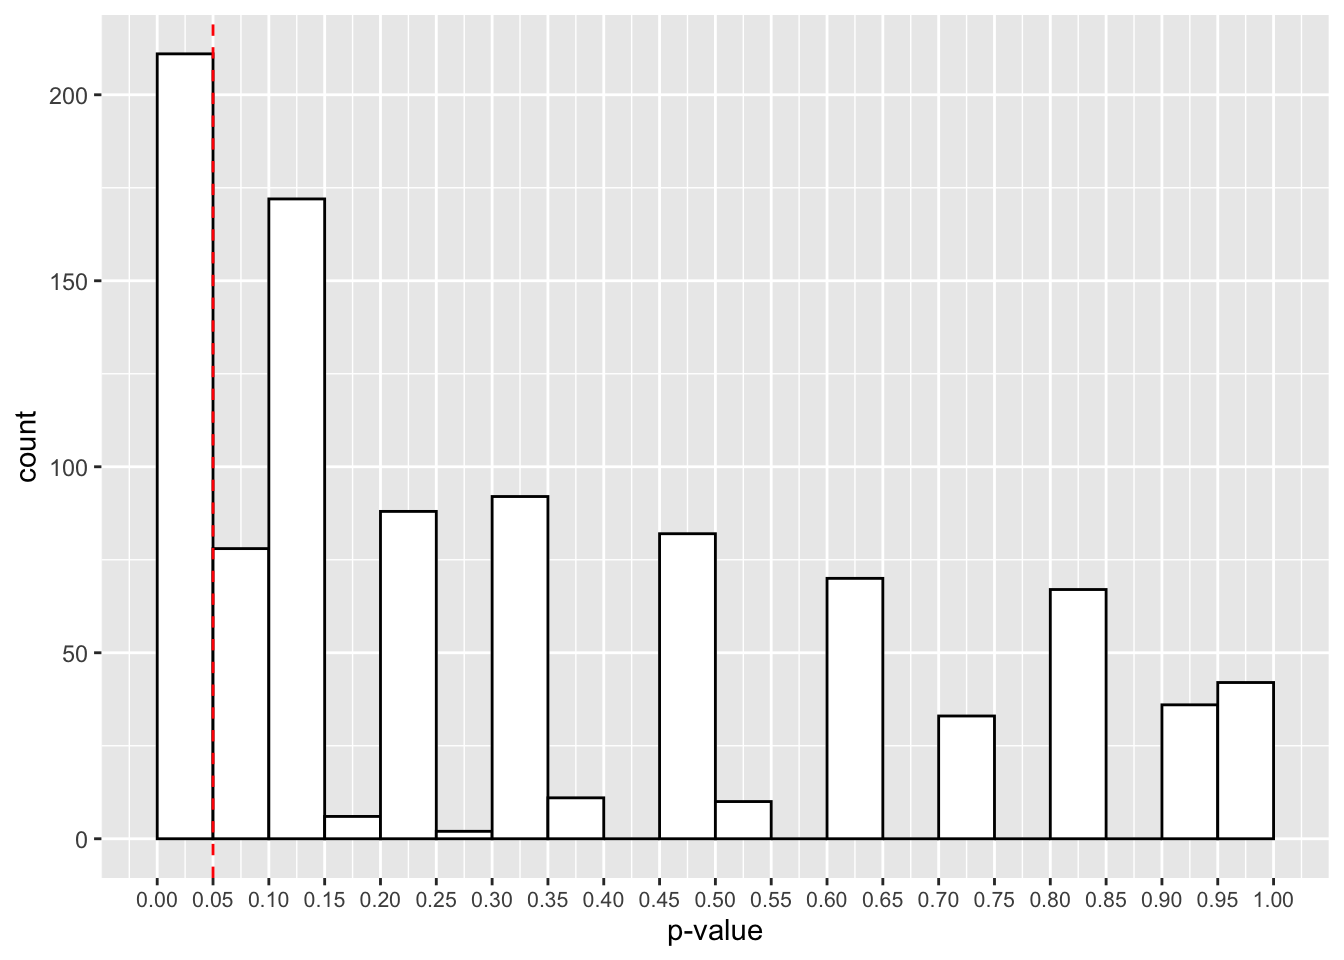
\includegraphics{r4psych_files/figure-latex/8_function_type_II_plot-1.pdf}

Now it looks like we have a much larger proportion of studies that give us \emph{p}-values below 0.05. Actually, it's 211, or 21.1\%.

What does this tell us? Actually, this is the power of our study, or the probability for us to detect a true effect when it is present in the population. As such, 1-power is the type-II error rate, or the probability to reject the alternative hypothesis when a true effect is present in the population.

At only 21.1\%, this is inadequate for our purposes. We generally aim for at least 80\% in psychological research. Here we have a much larger chance of committing a type-II error, or incorrectly rejecting the alternative hypothesis when there is a true effect in the population.

We can use this simulating method to help determine the parameters of our study. Let's look into increasing the sample size in our study, or the number of observations we make during the experiment.

\begin{Shaded}
\begin{Highlighting}[]
\NormalTok{true\_effect\_simulations }\OtherTok{\textless{}{-}} \FunctionTok{replicate}\NormalTok{(}\AttributeTok{n =} \DecValTok{1000}\NormalTok{, }
                         \FunctionTok{simulate\_psychic\_test}\NormalTok{(}\AttributeTok{n\_trials =} \DecValTok{600}\NormalTok{, }
                                               \AttributeTok{prob\_success =} \FloatTok{0.2}\NormalTok{,}
                                               \AttributeTok{psychic\_success =} \FloatTok{0.25}
\NormalTok{                                               )}
\NormalTok{                         )}
\end{Highlighting}
\end{Shaded}

\begin{Shaded}
\begin{Highlighting}[]
\FunctionTok{ggplot}\NormalTok{() }\SpecialCharTok{+} 
  \FunctionTok{geom\_histogram}\NormalTok{(}\FunctionTok{aes}\NormalTok{(true\_effect\_simulations),}
                 \AttributeTok{binwidth =} \FloatTok{0.05}\NormalTok{,}
                 \AttributeTok{boundary =} \DecValTok{0}\NormalTok{,}
                 \AttributeTok{fill =} \StringTok{"white"}\NormalTok{,}
                 \AttributeTok{colour =} \StringTok{"black"}\NormalTok{) }\SpecialCharTok{+}
  \FunctionTok{scale\_x\_continuous}\NormalTok{(}\AttributeTok{limits =} \FunctionTok{c}\NormalTok{(}\DecValTok{0}\NormalTok{, }\DecValTok{1}\NormalTok{), }
                     \AttributeTok{breaks =} \FunctionTok{seq}\NormalTok{(}\AttributeTok{from =} \DecValTok{0}\NormalTok{, }\AttributeTok{to =} \DecValTok{1}\NormalTok{, }\AttributeTok{by =} \FloatTok{0.05}\NormalTok{)}
\NormalTok{                     ) }\SpecialCharTok{+}
  \FunctionTok{geom\_vline}\NormalTok{(}\AttributeTok{xintercept =} \FloatTok{0.05}\NormalTok{, }\AttributeTok{linetype =} \DecValTok{2}\NormalTok{, }\AttributeTok{colour =} \StringTok{"red"}\NormalTok{) }\SpecialCharTok{+}
  \FunctionTok{labs}\NormalTok{(}\AttributeTok{x =} \StringTok{"p{-}value"}\NormalTok{) }\SpecialCharTok{+}
  \FunctionTok{theme}\NormalTok{(}\AttributeTok{axis.text.x =} \FunctionTok{element\_text}\NormalTok{(}\AttributeTok{size=}\DecValTok{8}\NormalTok{))}
\end{Highlighting}
\end{Shaded}

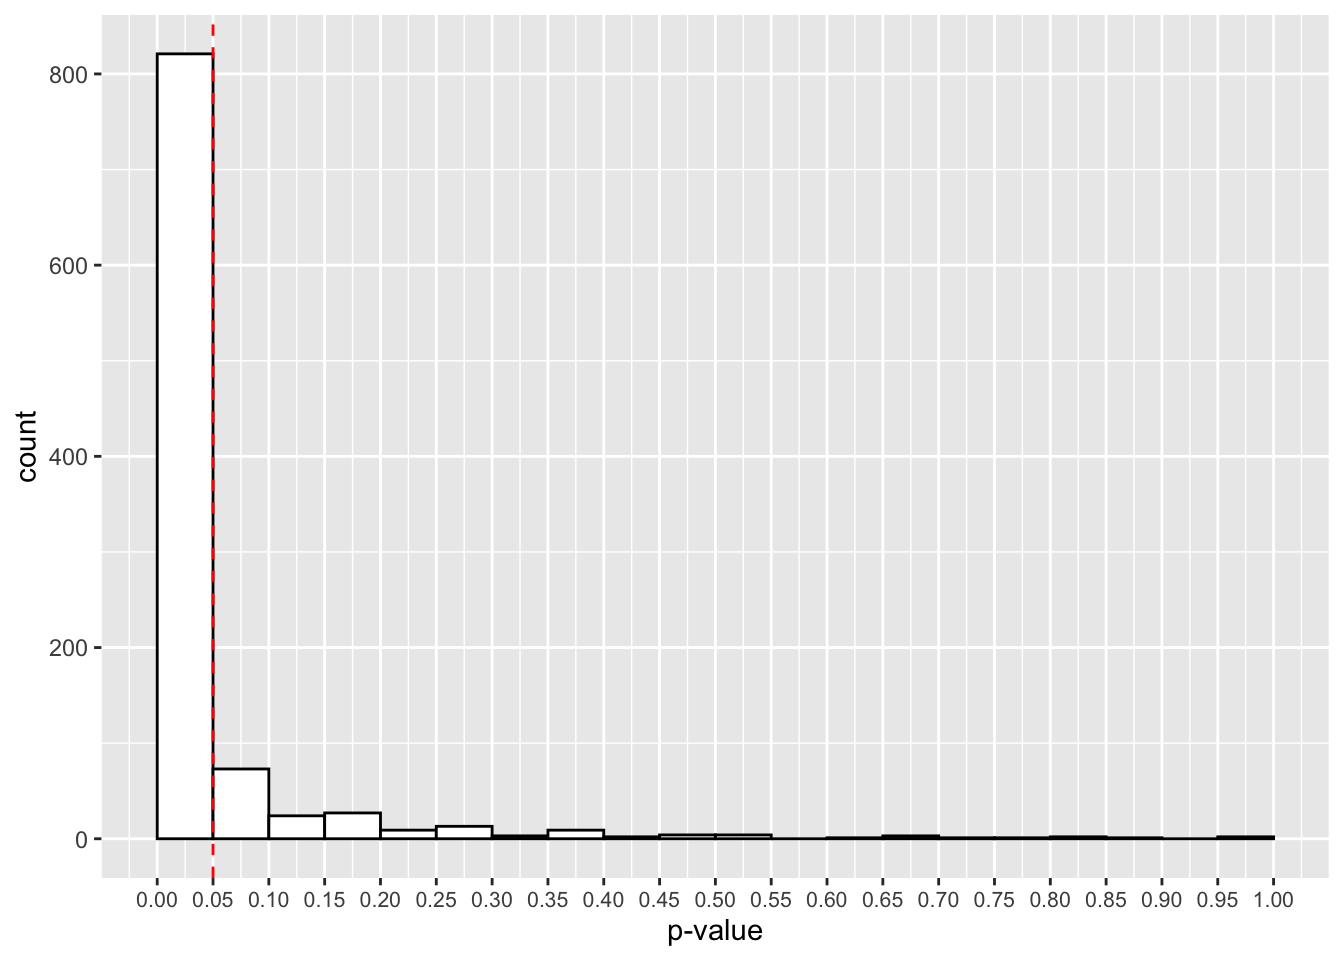
\includegraphics{r4psych_files/figure-latex/8_do_function_type_II_power_plot-1.pdf}

That looks better! Now, in most experiments, we'll get a \emph{p}-value below 0.05. How many studies detected this true effect? Our power for this study is:

\begin{Shaded}
\begin{Highlighting}[]
\FunctionTok{mean}\NormalTok{(true\_effect\_simulations }\SpecialCharTok{\textless{}} \FloatTok{0.05}\NormalTok{)}
\end{Highlighting}
\end{Shaded}

\begin{verbatim}
## [1] 0.821
\end{verbatim}

Great, at 600 trials we now have an 82.1\% chance to detect a true effect if present. It looks like we'll have one tired psychic by the end of this experiment!

As long as you can construct data that fits the form of your planned experiment you can use simulation to calculate the predicted power under the parameters that you set. \href{https://youtu.be/avHLWnX2ehQ}{As long as we have \emph{t}}- or \emph{p}-values to capture, we can simulate data, fit our model, and count the number of \emph{p}-values below our threshold (or \emph{t}-values above our threshold) where we reject the null hypothesis in order to come up with the power of our study. Typically, around 1000 samples is enough for this.

\hypertarget{flexible-power-analyses-with-simulation}{%
\subsection{Flexible Power Analyses with Simulation}\label{flexible-power-analyses-with-simulation}}

\hypertarget{simulation-for-simple-designs}{%
\subsubsection{Simulation for Simple Designs}\label{simulation-for-simple-designs}}

Now we understand how we can use simulation to create data sets and observe the probability that we'll detect a true effect with a simple design, we can build on our knowledge to look at more complex designs.

Let's return to the IQ study data. Remember, that the IQ test has a mean of 100 and standard deviation of 15. Let's run a power analysis to detect whether a predicted sample of people differ from this average range.

\begin{Shaded}
\begin{Highlighting}[]
\NormalTok{calculate\_IQ\_power }\OtherTok{\textless{}{-}} \ControlFlowTok{function}\NormalTok{(n, sample\_mean, sample\_sd, pop\_mean, pop\_sd) \{}
\NormalTok{  sample\_data }\OtherTok{\textless{}{-}} \FunctionTok{rnorm}\NormalTok{(}\AttributeTok{n =}\NormalTok{ n, }\AttributeTok{mean =}\NormalTok{ sample\_mean, }\AttributeTok{sd =}\NormalTok{ sample\_sd)}
\NormalTok{  test }\OtherTok{\textless{}{-}} \FunctionTok{t.test}\NormalTok{(sample\_data, }\AttributeTok{mu =}\NormalTok{ pop\_mean, }\AttributeTok{sd =}\NormalTok{ pop\_sd)}
\NormalTok{  test}\SpecialCharTok{$}\NormalTok{p.value}
\NormalTok{\}}
\end{Highlighting}
\end{Shaded}

Now let's run our function, replicated 1000 times. We'll sample assuming our population and sample have the same standard deviation, but the sample mean is 5 points higher than the general population. Finally, we'll sample 60 people.

We'll then calculate the mean number of \emph{p}-values below our 0.05 cut off point to see our power.

\begin{Shaded}
\begin{Highlighting}[]
\NormalTok{p\_vals }\OtherTok{\textless{}{-}} \FunctionTok{replicate}\NormalTok{(}\DecValTok{1000}\NormalTok{, }\FunctionTok{calculate\_IQ\_power}\NormalTok{(}\DecValTok{60}\NormalTok{, }\DecValTok{105}\NormalTok{, }\DecValTok{15}\NormalTok{, }\DecValTok{100}\NormalTok{, }\DecValTok{15}\NormalTok{))}
\FunctionTok{mean}\NormalTok{(p\_vals }\SpecialCharTok{\textless{}} \FloatTok{0.05}\NormalTok{)}
\end{Highlighting}
\end{Shaded}

\begin{verbatim}
## [1] 0.735
\end{verbatim}

Great, 73.5\% power is not bad at all. Maybe we should bump up the sample size a little to get to 80\%.

\begin{Shaded}
\begin{Highlighting}[]
\NormalTok{p\_vals }\OtherTok{\textless{}{-}} \FunctionTok{replicate}\NormalTok{(}\DecValTok{1000}\NormalTok{, }\FunctionTok{calculate\_IQ\_power}\NormalTok{(}\DecValTok{75}\NormalTok{, }\DecValTok{105}\NormalTok{, }\DecValTok{15}\NormalTok{, }\DecValTok{100}\NormalTok{, }\DecValTok{15}\NormalTok{))}
\FunctionTok{mean}\NormalTok{(p\_vals }\SpecialCharTok{\textless{}} \FloatTok{0.05}\NormalTok{)}
\end{Highlighting}
\end{Shaded}

\begin{verbatim}
## [1] 0.835
\end{verbatim}

It looks like around 75 participants does a good job for us. What if the standard deviation for our sample was smaller? i.e.~what if the samples tend to be more similar in their mean scores?

\begin{Shaded}
\begin{Highlighting}[]
\NormalTok{p\_vals }\OtherTok{\textless{}{-}} \FunctionTok{replicate}\NormalTok{(}\DecValTok{1000}\NormalTok{, }\FunctionTok{calculate\_IQ\_power}\NormalTok{(}\DecValTok{20}\NormalTok{, }\DecValTok{105}\NormalTok{, }\FloatTok{7.5}\NormalTok{, }\DecValTok{100}\NormalTok{, }\DecValTok{15}\NormalTok{))}
\FunctionTok{mean}\NormalTok{(p\_vals }\SpecialCharTok{\textless{}} \FloatTok{0.05}\NormalTok{)}
\end{Highlighting}
\end{Shaded}

\begin{verbatim}
## [1] 0.82
\end{verbatim}

Now it looks like we only need around 20 participants to achieve the same power.

What if the mean score is half as large as before?

\begin{Shaded}
\begin{Highlighting}[]
\NormalTok{p\_vals }\OtherTok{\textless{}{-}} \FunctionTok{replicate}\NormalTok{(}\DecValTok{1000}\NormalTok{, }\FunctionTok{calculate\_IQ\_power}\NormalTok{(}\DecValTok{70}\NormalTok{, }\FloatTok{102.5}\NormalTok{, }\FloatTok{7.5}\NormalTok{, }\DecValTok{100}\NormalTok{, }\DecValTok{15}\NormalTok{))}
\FunctionTok{mean}\NormalTok{(p\_vals }\SpecialCharTok{\textless{}} \FloatTok{0.05}\NormalTok{)}
\end{Highlighting}
\end{Shaded}

\begin{verbatim}
## [1] 0.793
\end{verbatim}

Now we need more participants, even though the standard deviation is as small as before.

As you can see, sample size, effect sizes, and variance all affect the ability to detect a true effect.

\hypertarget{simulation-for-more-complex-designs}{%
\subsubsection{Simulation for More Complex Designs}\label{simulation-for-more-complex-designs}}

So far, we've looked at simulation for cases where we have a baseline condition to compare against. However, we often want to compare to or more groups against one another to determine if they differ on some outcome variable. For a \emph{t}-test, this is as simple as sampling two sets of data using \texttt{rnorm()} and comparing the two against one another. However, we'll look at a more complex 2 by 2 between-subjects design, which can be adapted to most scenarios.

Here, participants take part in 1 combination of 2 factors (A and B) each with 2 levels. To get started we first have to create a tibble to hold our simulated data.

\begin{Shaded}
\begin{Highlighting}[]
\CommentTok{\# how many subjects?}
\NormalTok{n }\OtherTok{\textless{}{-}} \DecValTok{60}

\CommentTok{\# create your design}
\NormalTok{design }\OtherTok{\textless{}{-}} \FunctionTok{expand.grid}\NormalTok{(}\AttributeTok{A =} \FunctionTok{c}\NormalTok{(}\SpecialCharTok{{-}}\NormalTok{.}\DecValTok{5}\NormalTok{, .}\DecValTok{5}\NormalTok{), }\AttributeTok{B =} \FunctionTok{c}\NormalTok{(}\SpecialCharTok{{-}}\NormalTok{.}\DecValTok{5}\NormalTok{, .}\DecValTok{5}\NormalTok{))}

\CommentTok{\# create table of data}
\NormalTok{data }\OtherTok{\textless{}{-}} \FunctionTok{tibble}\NormalTok{(}\AttributeTok{subject =} \DecValTok{1}\SpecialCharTok{:}\NormalTok{ n,}
               \AttributeTok{A =} \FunctionTok{rep}\NormalTok{(design}\SpecialCharTok{$}\NormalTok{A, n}\SpecialCharTok{/}\DecValTok{4}\NormalTok{),}
               \AttributeTok{B =} \FunctionTok{rep}\NormalTok{(design}\SpecialCharTok{$}\NormalTok{B, n}\SpecialCharTok{/}\DecValTok{4}\NormalTok{)}
\NormalTok{               )}

\CommentTok{\# look at the data}
\NormalTok{data}
\end{Highlighting}
\end{Shaded}

\begin{verbatim}
## # A tibble: 60 x 3
##    subject     A     B
##      <int> <dbl> <dbl>
##  1       1  -0.5  -0.5
##  2       2   0.5  -0.5
##  3       3  -0.5   0.5
##  4       4   0.5   0.5
##  5       5  -0.5  -0.5
##  6       6   0.5  -0.5
##  7       7  -0.5   0.5
##  8       8   0.5   0.5
##  9       9  -0.5  -0.5
## 10      10   0.5  -0.5
## # ... with 50 more rows
\end{verbatim}

Notice that we defined our two condition columns with the values of -.5 and .5. Think back to how this is modelled in a linear model in R. What might the intercept term be? It will be the mean across both conditions.

Next, we need to set up the coefficients and error term for our model. We want the intercept to be 400, a shift in A to be the intercept + 30, a shift in B to be the intercept - 50, and the interaction term to be the intercept - 40. Finally, our error term has a mean of 0 and standard deviation of 40.

We then create our data using the formula for the linear model, and add this to our data.

\begin{Shaded}
\begin{Highlighting}[]
\CommentTok{\# set up coefficients}
\NormalTok{alpha }\OtherTok{=} \DecValTok{400}
\NormalTok{beta1 }\OtherTok{=} \DecValTok{30}
\NormalTok{beta2 }\OtherTok{=} \SpecialCharTok{{-}}\DecValTok{50}
\NormalTok{beta3 }\OtherTok{=} \SpecialCharTok{{-}}\DecValTok{40}
\NormalTok{err }\OtherTok{\textless{}{-}} \FunctionTok{rnorm}\NormalTok{(n, }\DecValTok{0}\NormalTok{, }\AttributeTok{sd =} \DecValTok{40}\NormalTok{)}

\CommentTok{\# create data from the linear model}
\NormalTok{data}\SpecialCharTok{$}\NormalTok{y }\OtherTok{\textless{}{-}}\NormalTok{ alpha }\SpecialCharTok{+}\NormalTok{ (beta1}\SpecialCharTok{*}\NormalTok{data}\SpecialCharTok{$}\NormalTok{A) }\SpecialCharTok{+}\NormalTok{ (beta2}\SpecialCharTok{*}\NormalTok{data}\SpecialCharTok{$}\NormalTok{B) }\SpecialCharTok{+}\NormalTok{ (beta3}\SpecialCharTok{*}\NormalTok{data}\SpecialCharTok{$}\NormalTok{A}\SpecialCharTok{*}\NormalTok{data}\SpecialCharTok{$}\NormalTok{B) }\SpecialCharTok{+}\NormalTok{ err}

\CommentTok{\# see the data}
\NormalTok{data}
\end{Highlighting}
\end{Shaded}

\begin{verbatim}
## # A tibble: 60 x 4
##    subject     A     B     y
##      <int> <dbl> <dbl> <dbl>
##  1       1  -0.5  -0.5  421.
##  2       2   0.5  -0.5  472.
##  3       3  -0.5   0.5  408.
##  4       4   0.5   0.5  443.
##  5       5  -0.5  -0.5  423.
##  6       6   0.5  -0.5  479.
##  7       7  -0.5   0.5  405.
##  8       8   0.5   0.5  386.
##  9       9  -0.5  -0.5  498.
## 10      10   0.5  -0.5  428.
## # ... with 50 more rows
\end{verbatim}

Let's see how this data would look when modelled.

\begin{Shaded}
\begin{Highlighting}[]
\NormalTok{fit }\OtherTok{\textless{}{-}} \FunctionTok{lm}\NormalTok{(y }\SpecialCharTok{\textasciitilde{}}\NormalTok{ A }\SpecialCharTok{*}\NormalTok{ B, }\AttributeTok{data =}\NormalTok{ data)}
\FunctionTok{summary}\NormalTok{(fit)}
\end{Highlighting}
\end{Shaded}

\begin{verbatim}
## 
## Call:
## lm(formula = y ~ A * B, data = data)
## 
## Residuals:
##      Min       1Q   Median       3Q      Max 
## -108.540  -30.991    8.045   24.951   89.673 
## 
## Coefficients:
##             Estimate Std. Error t value Pr(>|t|)    
## (Intercept)  401.193      5.694  70.456  < 2e-16 ***
## A             17.397     11.388   1.528   0.1322    
## B            -55.695     11.388  -4.890 8.85e-06 ***
## A:B          -47.358     22.777  -2.079   0.0422 *  
## ---
## Signif. codes:  0 '***' 0.001 '**' 0.01 '*' 0.05 '.' 0.1 ' ' 1
## 
## Residual standard error: 44.11 on 56 degrees of freedom
## Multiple R-squared:  0.3532, Adjusted R-squared:  0.3185 
## F-statistic: 10.19 on 3 and 56 DF,  p-value: 1.868e-05
\end{verbatim}

Finally, we need to fit a model to our simulated data and extract the \emph{p}-value. We need to do this fitting and extracting process several times before we can calculate our power to detect an effect. However, we need to know which effect we're interested in detecting. Is it just an effect of A, B, or the interaction? That choice is up to you, but for now we'll simply look at the probability to detect an effect for the interaction.

Thankfully, we can save on writing long functions and/or loops when we have some data like this by fitting our model once, and then using the \texttt{simulate()} function in R.

In this function, we need to pass our original data and model fit. We then create new data from our original data, but with a simulated response variable (\texttt{sim\_y}) made from the \texttt{simulate()} function which is applied to our original model. We then refit the model with our new data and response variable, and we use a helper function \texttt{broom::tidy()} which puts model outputs in a nice table so we can easily select the \emph{p}-value for the 4th row (i.e.~the interaction). Try running \texttt{str()} on both \textbf{fit} and \textbf{tidy\_table} to see what I mean.

\begin{Shaded}
\begin{Highlighting}[]
\NormalTok{simulate\_model\_fit }\OtherTok{\textless{}{-}} \ControlFlowTok{function}\NormalTok{(data, model\_fit) \{}
  \CommentTok{\# simulate data and add to tibble}
\NormalTok{  new\_data }\OtherTok{\textless{}{-}} \FunctionTok{mutate}\NormalTok{(data, }\AttributeTok{sim\_y =} \FunctionTok{simulate}\NormalTok{(fit)}\SpecialCharTok{$}\NormalTok{sim\_1)}
  
  \CommentTok{\# refit model}
\NormalTok{  refit\_model }\OtherTok{\textless{}{-}} \FunctionTok{lm}\NormalTok{(sim\_y }\SpecialCharTok{\textasciitilde{}}\NormalTok{ A }\SpecialCharTok{*}\NormalTok{ B, }\AttributeTok{data =}\NormalTok{ new\_data)}
  
  \CommentTok{\# extract p{-}value for interaction}
\NormalTok{  broom}\SpecialCharTok{::}\FunctionTok{tidy}\NormalTok{(refit\_model)}\SpecialCharTok{$}\NormalTok{p.value[}\DecValTok{4}\NormalTok{]}
\NormalTok{\}}
\end{Highlighting}
\end{Shaded}

Finally, we can use \texttt{replicate()} to do this process however many times we'd like. We then calculate the power by seeing how often we find \emph{p}-values below 0.05 for the interaction term.

\begin{Shaded}
\begin{Highlighting}[]
\NormalTok{complex\_power }\OtherTok{\textless{}{-}} \FunctionTok{replicate}\NormalTok{(}\DecValTok{1000}\NormalTok{, }\FunctionTok{simulate\_model\_fit}\NormalTok{(data, fit))}
\FunctionTok{mean}\NormalTok{(complex\_power }\SpecialCharTok{\textless{}}\NormalTok{ .}\DecValTok{05}\NormalTok{)}
\end{Highlighting}
\end{Shaded}

\begin{verbatim}
## [1] 0.529
\end{verbatim}

Nice, we have very high power for this study!

Feel free to reuse and adapt the script above to your own needs. Try looking at the impact of inputting different parameter estimates and designs.

\hypertarget{performing-power-analyses-from-packages}{%
\section{Performing Power Analyses from Packages}\label{performing-power-analyses-from-packages}}

The first option of calculating power through simulation is very flexible, and I think it helps you to think more deeply about your data when compared to running canned power analyses. Also, there aren't many ways to easily calculate power with mixed effects models, and so simulation is our best bet at the moment. However, there are options out there if you want to calculate power for most designs without the need to do simulation.

R has an inbuilt power analysis function for \emph{t}-tests called \texttt{power.t.test()}, and for ANOVAs called \texttt{power.anova.test()}.

Let's see how the ANOVA function works, and you can work back to the \emph{t}-test function if necessary. In this function, we just have to define the number of groups we have, the number of observations in each group (typically participants in psychology), and the variance for any between-subjects and within-subjects variables.

Making the below assumptions, it looks like our study is overpowered.

\begin{Shaded}
\begin{Highlighting}[]
\FunctionTok{power.anova.test}\NormalTok{(}\AttributeTok{groups =} \DecValTok{4}\NormalTok{, }\AttributeTok{n =} \DecValTok{20}\NormalTok{, }\AttributeTok{between.var =} \DecValTok{1}\NormalTok{, }\AttributeTok{within.var =} \DecValTok{3}\NormalTok{)}
\end{Highlighting}
\end{Shaded}

\begin{verbatim}
## 
##      Balanced one-way analysis of variance power calculation 
## 
##          groups = 4
##               n = 20
##     between.var = 1
##      within.var = 3
##       sig.level = 0.05
##           power = 0.9679022
## 
## NOTE: n is number in each group
\end{verbatim}

Alternatively, we can predefine our desired power (typically 80\% in psychology), and this will work out the number of participants needed per group.

\begin{Shaded}
\begin{Highlighting}[]
\FunctionTok{power.anova.test}\NormalTok{(}\AttributeTok{groups =} \DecValTok{4}\NormalTok{, }\AttributeTok{between.var =} \DecValTok{1}\NormalTok{, }\AttributeTok{within.var =} \DecValTok{3}\NormalTok{, }\AttributeTok{power =}\NormalTok{ .}\DecValTok{80}\NormalTok{)}
\end{Highlighting}
\end{Shaded}

\begin{verbatim}
## 
##      Balanced one-way analysis of variance power calculation 
## 
##          groups = 4
##               n = 11.92613
##     between.var = 1
##      within.var = 3
##       sig.level = 0.05
##           power = 0.8
## 
## NOTE: n is number in each group
\end{verbatim}

Great, it looks like we only need 12 people in each group to achieve a power of 80\%.

There are other options which allow you to specify means or effect sizes to determine power, and as such these may be more user friendly. One option is the \texttt{pwr} package, which contains a number of functions for calcualting power with different designs. Have a look at this in your own time to see if it will be useful to you.

\hypertarget{exercises-7}{%
\section{Exercises}\label{exercises-7}}

\hypertarget{introduction-and-setup-1}{%
\subsection{Introduction and Setup}\label{introduction-and-setup-1}}

For these exercises, we will look at the core concepts from this lesson. Here, you'll make your own data using simulation-based techniques, and you'll use those same techniques to calculate power for your design.

\hypertarget{question-1-7}{%
\subsection{Question 1}\label{question-1-7}}

Create some data for 60 participants (split into two groups), A and B. Save this as a tibble called \textbf{sim\_data}.

Make a column containing the subject ID (called \textbf{subject\_id}), a column for condition (called \textbf{condition}), and a column for the outcome (called \textbf{outcome}).

You will have to use the \texttt{seq()} function to make sequential numbers for the subject ID, the \texttt{rep()} function with the \texttt{c()} function to make the conditions, and the \texttt{rnorm()} function with the \texttt{c()} function to make the scores.

For the outcome column, we want a mean of 180, and standard deviation of 10 for the first group, and a mean of 190 and standard deviation of 10 for the second group.

\hypertarget{question-2-7}{%
\subsection{Question 2}\label{question-2-7}}

Generate summary statistics for the data set. We want means, SDs, and ns for the table of summary statistics. How do these means and standard deviations match the sampling procedure? Are you surprised at all by these values?

\hypertarget{question-3-7}{%
\subsection{Question 3}\label{question-3-7}}

Conduct an independent samples \emph{t}-test looking at differences in the scores across the two groups.

\hypertarget{question-4-7}{%
\subsection{Question 4}\label{question-4-7}}

Turn the sampling procedure into a function called \texttt{sim\_data}.

The arguments the function can take are:

\begin{itemize}
\tightlist
\item
  n\_one: the number of observations for group 1
\item
  n\_two: the number of observations for group 2
\item
  mean\_one: the mean score in the population for group 1
\item
  mean\_two: the mean score in the population for group 2
\item
  sd\_one: the standard deviation in the population for group 1
\item
  sd\_two: the standard deviation in the population for group 2
\end{itemize}

Remember that these arguments come within the paretheses after the blue \texttt{function} part.

\emph{Hint}: Just copy and paste your code for 1, and replace the things you want to vary with the name of a variable that will define your function arguments.

Test that your function works by passing it some parameters. Pass it an n of 80 for both groups, a mean of 200 and SD of 10 for group 1, and a mean of 195 and SD for 10 for group 2.

Assign the outcome of your function to an object to save the outcome. Call this object \textbf{new\_data}.

\hypertarget{question-5-7}{%
\subsection{Question 5}\label{question-5-7}}

Make a new function called \texttt{sim\_test}, which uses your simulation function from above to make some data before it runs an independent samples \emph{t}-test on the data. Finally, this function should output the \emph{p}-value from the \emph{t}-test. Note that this function should take as arguments the same arguments from the function in question 4. Can you figure out why this is the case?

Test that your function works by passing it the same arguments as in question 4, and assign this to the object \texttt{new\_data\_p}.

\hypertarget{question-6-7}{%
\subsection{Question 6}\label{question-6-7}}

Calculate the power for your study based on the parameters from question 4 and 5 (ns of 80; mean of 200 and 195, SDs of 10). Do so by running your function 1000 times and capturing the p-values. Assign this to the object \textbf{power\_data}.

\emph{Top Tip}: If you need to test your code (which you should), make sure you use a low number like 10 for your replications before running it 1000 times to answer this question. This will save time and avoid flooding your console etc. if you make a mistake.

\hypertarget{question-7-6}{%
\subsection{Question 7}\label{question-7-6}}

Calculate the power of your study from the \emph{p}-values in question 6. What is the power for your study? (Your values will differ from mine as we aren't using \texttt{set.seed()}, but we're instead using proper random sampling.)

\hypertarget{question-8-6}{%
\subsection{Question 8}\label{question-8-6}}

Make a plot of the \emph{p}-values from your simulated data. Make this with a binwidth of 0.05, a boundary of 0 and with white bars with a black border.

Also, make sure that the breaks happen at every 0.05 tick along the x-axis.

What percentage of your data lie below the 0.05 line? What does this correspond to?

\hypertarget{question-9-6}{%
\subsection{Question 9}\label{question-9-6}}

Remake your data from question 6, only with means of 200 in each group. Call this \textbf{power\_data\_null}.

Then calculate the power as in question 7, and plot your data as in question 8.

\emph{Note}: The sampling procedure may take a while to run.

What percentage of the data fall below the 0.05 line on the plot? What does this correspond to? What percentage falls within each bin above the 0.05 line? Are you surprised at the distribution of the \emph{p}-values?

\hypertarget{mixed-effects-models}{%
\chapter{Mixed Effects Models}\label{mixed-effects-models}}

In this session we'll cover Linear/Hierarchical Mixed Effects Modelling. We'll cover why you should use mixed effects modelling for your own analyses, how these models work, and how to define your models properly in R. Specifically, we'll cover:

\begin{itemize}
\tightlist
\item
  Fixed and Random Effects
\item
  Random Intercepts and Slopes
\item
  Nested and Crossed Random Effects
\item
  Partial-Pooling of Data
\item
  Calculating \emph{p}-values
\item
  Generalised Mixed Effects Models
\end{itemize}

One nice introduction to mixed effects models is provided by Bodo Winter in two parts: \href{http://www.bodowinter.com/tutorial/bw_LME_tutorial1.pdf}{part one} and \href{http://www.bodowinter.com/tutorial/bw_LME_tutorial2.pdf}{part two} and you might want to check this out as further reading from this chapter.

\hypertarget{getting-started-6}{%
\section{Getting Started}\label{getting-started-6}}

As always, we first need to load the \texttt{tidyverse} set of package. However, for this chapter we also need the \texttt{lme4} package. This package allows us to run mixed effects models in R using the \texttt{lmer} and \texttt{glmer} commands for linear mixed effects models and generalised linear mixed effects models respectively. These models are similar to linear models and generalised lienar models in that the first can take continuous, unbounded data, and the second takes bounded, discrete data.

\begin{Shaded}
\begin{Highlighting}[]
\CommentTok{\# load packages}
\FunctionTok{library}\NormalTok{(tidyverse)}
\FunctionTok{library}\NormalTok{(lme4)}
\end{Highlighting}
\end{Shaded}

Additionally, we'll load the data set for this study. This is the inbuilt \texttt{sleepstudy} data set from \texttt{lme4}, but I've simulated 2 additional participants before removing a lot of their observations. This is to show you just how powerful mixed effects models are when we have missing data.

\hypertarget{why-mixed-effects-models}{%
\section{Why Mixed Effects Models}\label{why-mixed-effects-models}}

In all of the previous analyses we've used so far, our models have assumed that we have independence between cases in our data. However, this assumption is often violated, which can cause some serious problems when it comes to interpreting our tests.

Let's assume we're interested in language learning in children from monolinguial and bilingual backgrounds. We may decide to test how well children learn an artificial language by going to several schools and testing children in the same year group from different classes.

If we fit a traditional linear model to our data, we implicitly make the assumption that learning should be the same regardless of the class or school the child attends. Yet we know this is unlikely to be true; schools reflect the demographics of an area and the school ethos, and individual teachers may be better or worse at teaching linguistics to children. This means that children within the same school are likely to be more similar to one another than to children from different schools. Moreover, children within the class are likely to be more similar to one another than to children in different classes. In this way, our data should be nested such that children should be defined as part of a specific class in a specific school, and our models should reflect this ordering.

With mixed effects models, we can directly model this dependency in our data. Moreover, mixed effects models make fewer strict assumptions to other tests (\citet{field2012discovering}), such as:

\begin{itemize}
\item
  Homogeneity of regression slopes: Mixed effects models can directly model variability in slopes, so we needn't make any assumption that slopes are similar across conditions (which is often untrue).
\item
  Assumption of independence: with independent-samples tests we often assume that data are unrelated to one-another. But again, this is often not the case; take learning over time. The same person provides multiple measurements at multiple time points. Mixed effects models can handle this well.
\item
  Complete data: Often, with traditional analyses you just have to throw away entire sources of data (e.g.~participants) if one case (e.g.~one trial) is missing. This isn't the case with mixed effects models, where we can estimate missing data based on what we have available to us.
\end{itemize}

For these reasons, by default you should probably pick mixed effects models to model your data.

\hypertarget{how-do-mixed-effects-models-work}{%
\section{How Do Mixed Effects Models Work?}\label{how-do-mixed-effects-models-work}}

\hypertarget{fixed-and-random-effects}{%
\subsection{Fixed and Random Effects}\label{fixed-and-random-effects}}

So far, we've only talked about our parameter estimates from a linear model in terms of factors and levels. However, you can also consider the factors in your study in terms of whether they are fixed or random effects. Typically, a \textbf{fixed effect} will contain all possible levels of a factor in the experiment, while a \textbf{random effect} will be a random sample of possible levels of a factor. In effect, we can only generalise our fixed effects results to the levels within an experiment, but we can generalise from our random effects to levels beyond those that took part in our study.

Returning to our classroom example, if we tested languge learning in one of two conditions in students from different schools and and classes, our fixed effect would be the condition for the study. Hence, the random effects would be everything else we'd like to generalise to outside of our study. We probably want to generalise our results to all classes and all schools, so our random effects would be students within classes within schools.

In traditional models, you can say that all of the effects of interest, or the factors in the model, are defined as fixed effects. However, with mixed effects models, we can have both fixed and random effects in our model (hence \textbf{mixed effects} models).

To fit a mixed effects model, we simply define our fixed effects like we normally do for a linear model. However, there are different ways that we can define our random effects. Your choice of definition incorporates your belief of how the random effects work. Let's explore how the way in which we define our random effects influences our model fit.

\hypertarget{fixed-intercept-and-slope}{%
\subsubsection{Fixed Intercept and Slope}\label{fixed-intercept-and-slope}}

To look at how mixed effects models work, we'll use some toy data based on the \texttt{sleepstudy} data set from \textbf{lme4}. I made this quickly in another script, and you can load it using the code below.

This just makes three groups within our data, and we can look at this like conducting our study in three phases, with three different groups of people. As with the \texttt{sleepstudy} data set, this data set looks at the effect of days without sleep on reaction times.

\begin{Shaded}
\begin{Highlighting}[]
\NormalTok{sleep\_groups }\OtherTok{\textless{}{-}} \FunctionTok{read\_csv}\NormalTok{(}\StringTok{"inputs/sleep\_study\_with\_sim\_groups.csv"}\NormalTok{)}
\end{Highlighting}
\end{Shaded}

\begin{verbatim}
## Rows: 540 Columns: 4
## -- Column specification ------------------------------------
## Delimiter: ","
## chr (1): Group
## dbl (3): Reaction, Days, Subject
## 
## i Use `spec()` to retrieve the full column specification for this data.
## i Specify the column types or set `show_col_types = FALSE` to quiet this message.
\end{verbatim}

If we were to fit this data to a traditional linear model, and we ignored the fact that we have a random effect in our study (Group), then our linear model coefficients might look like this:

\begin{Shaded}
\begin{Highlighting}[]
\FunctionTok{lm}\NormalTok{(Reaction }\SpecialCharTok{\textasciitilde{}}\NormalTok{ Days, }\AttributeTok{data =}\NormalTok{ sleep\_groups)}
\end{Highlighting}
\end{Shaded}

\begin{verbatim}
## 
## Call:
## lm(formula = Reaction ~ Days, data = sleep_groups)
## 
## Coefficients:
## (Intercept)         Days  
##       371.7         15.4
\end{verbatim}

That is, we would get an intercept of approximately 351.5 and a slope of approximately 10.3 which is used to define the relationship for days on reaction times across all participants. This type of model looks against the raw data for the study looks like this:

\begin{Shaded}
\begin{Highlighting}[]
\FunctionTok{ggplot}\NormalTok{(}\AttributeTok{data =}\NormalTok{ sleep\_groups, }\AttributeTok{mapping =} \FunctionTok{aes}\NormalTok{(}\AttributeTok{x =}\NormalTok{ Days, }\AttributeTok{y =}\NormalTok{ Reaction)) }\SpecialCharTok{+}
  \FunctionTok{geom\_point}\NormalTok{(}\AttributeTok{na.rm =}\NormalTok{ T, }\FunctionTok{aes}\NormalTok{(}\AttributeTok{col =}\NormalTok{ Group), }\AttributeTok{alpha =} \FloatTok{0.5}\NormalTok{) }\SpecialCharTok{+}
  \FunctionTok{geom\_smooth}\NormalTok{(}\AttributeTok{method =} \StringTok{"lm"}\NormalTok{, }\AttributeTok{na.rm =}\NormalTok{ T, }\AttributeTok{col =} \StringTok{"black"}\NormalTok{, }\AttributeTok{se =}\NormalTok{ F) }\SpecialCharTok{+}
  \FunctionTok{scale\_y\_continuous}\NormalTok{(}\AttributeTok{limits =} \FunctionTok{c}\NormalTok{(}\DecValTok{180}\NormalTok{, }\DecValTok{1020}\NormalTok{)) }\SpecialCharTok{+}
  \FunctionTok{scale\_x\_continuous}\NormalTok{(}\AttributeTok{breaks =} \FunctionTok{seq}\NormalTok{(}\DecValTok{1}\SpecialCharTok{:}\DecValTok{10}\NormalTok{) }\SpecialCharTok{{-}} \DecValTok{1}\NormalTok{) }\SpecialCharTok{+}
  \FunctionTok{theme}\NormalTok{(}\AttributeTok{legend.position =} \StringTok{"top"}\NormalTok{)}
\end{Highlighting}
\end{Shaded}

\begin{verbatim}
## `geom_smooth()` using formula 'y ~ x'
\end{verbatim}

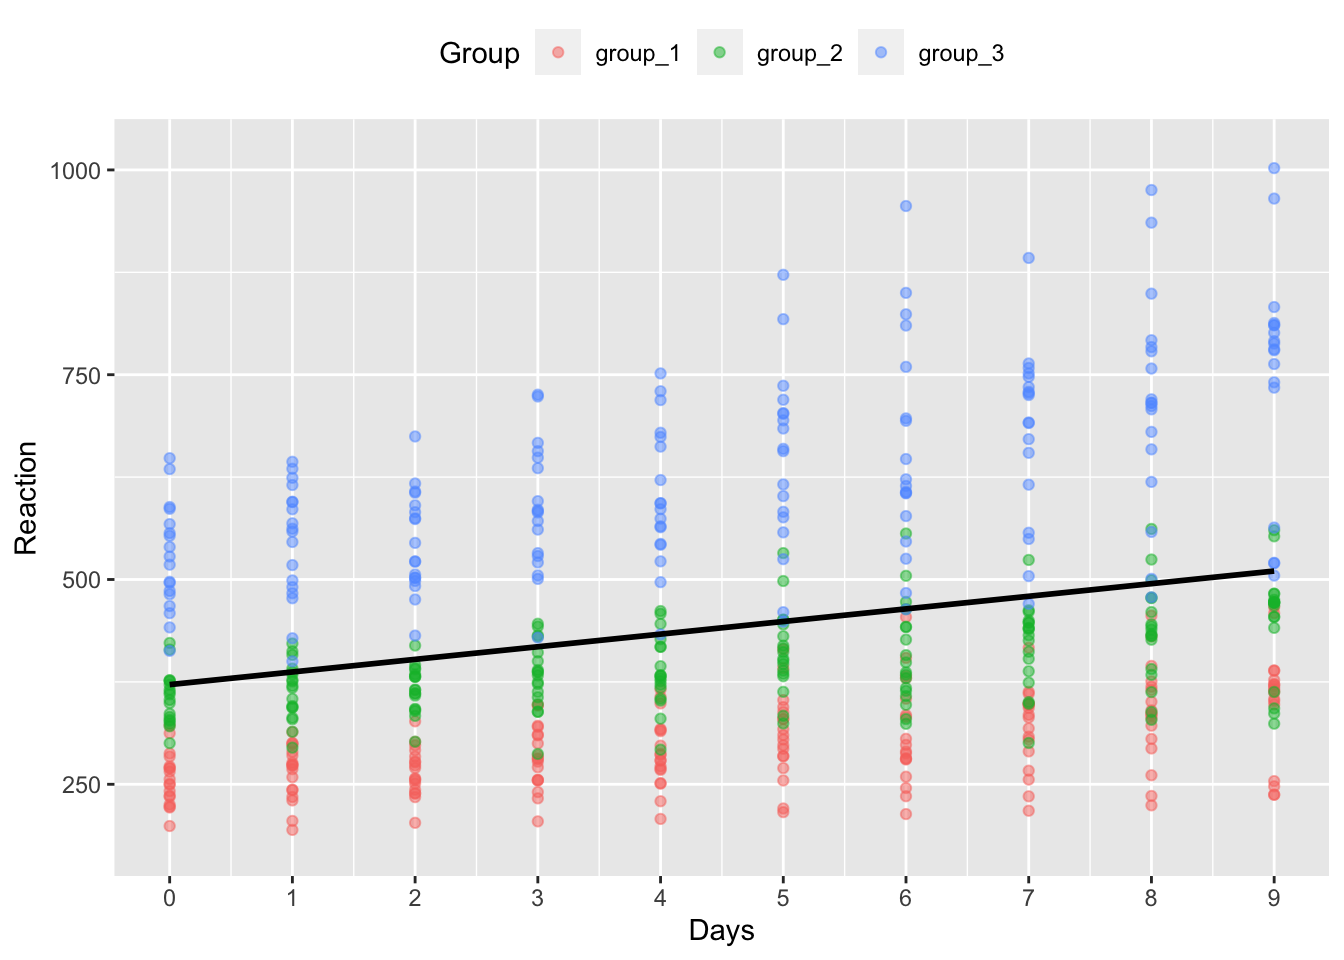
\includegraphics{r4psych_files/figure-latex/plot-lm-reaction-days-1.pdf}

But, you can see from the colour of the points that we have 3 distinct groups of participants in our model. It's clear that the three groups have different intercepts, and group 3 has a much steeper slope than the other two groups. Perhaps, then, we should model this difference across groups, even if it's not the main factor of interest in our study.

\hypertarget{random-intercepts}{%
\subsubsection{Random Intercepts}\label{random-intercepts}}

We define a mixed effects model in a similar way to a traditional linear model. Here, the only difference is we run the model using the \texttt{lmer()} function from \textbf{lme4}, rather than the \texttt{lm()} function from base R, and we specify our random effects as well.

\begin{Shaded}
\begin{Highlighting}[]
\CommentTok{\# fit random intercepts model}
\NormalTok{intercepts\_model }\OtherTok{\textless{}{-}} \FunctionTok{lmer}\NormalTok{(Reaction }\SpecialCharTok{\textasciitilde{}}\NormalTok{ Days }\SpecialCharTok{+}\NormalTok{ (}\DecValTok{1} \SpecialCharTok{|}\NormalTok{ Group), }\AttributeTok{data =}\NormalTok{ sleep\_groups)}
\end{Highlighting}
\end{Shaded}

As with regular linear models, we define our response variable as the column name to the left of the \texttt{\textasciitilde{}} (read: tilde). We then define our fixed effects to the right of the \texttt{\textasciitilde{}}.

After this, we define our random effects in parentheses. Here, we have specified that we want \textbf{random intercept (1)} for each group; \texttt{(1\ \textbar{}\ Group)}. Notice that we have a \texttt{\textbar{}} (read: pipe) between the 1 and group. This specifies what you want to calculate, by which random factor - here it is random intercepts (1) by the Group random factor.

Finally, as always we specify our data set, which should be in long format.

Let's see how defining random intercepts affects the coefficients for the groups in our model. We can extract model coefficients using the \texttt{coef()} function. I specifically got the Group coefficients by asking for this using the dollar notation after the function call. To make this easier on the eyes I've renamed the columns, and created an identifier for the intercepts and slopes (i.e.~the Group column).

\begin{Shaded}
\begin{Highlighting}[]
\CommentTok{\# see group coefficients}
\NormalTok{model\_coefs }\OtherTok{\textless{}{-}} \FunctionTok{coef}\NormalTok{(intercepts\_model)}\SpecialCharTok{$}\NormalTok{Group }\SpecialCharTok{\%\textgreater{}\%} 
  \FunctionTok{rename}\NormalTok{(}\AttributeTok{Intercept =} \StringTok{\textasciigrave{}}\AttributeTok{(Intercept)}\StringTok{\textasciigrave{}}\NormalTok{, }\AttributeTok{Slope =}\NormalTok{ Days) }\SpecialCharTok{\%\textgreater{}\%} 
  \FunctionTok{rownames\_to\_column}\NormalTok{(}\StringTok{"Group"}\NormalTok{)}

\CommentTok{\# see coefficients}
\NormalTok{model\_coefs}
\end{Highlighting}
\end{Shaded}

\begin{verbatim}
##     Group Intercept    Slope
## 1 group_1  229.3394 15.40385
## 2 group_2  329.0908 15.40385
## 3 group_3  556.6432 15.40385
\end{verbatim}

How would this model look against our raw data?

First, we'll join these coefficients to our original data so we can plot the individual lines.

\begin{Shaded}
\begin{Highlighting}[]
\NormalTok{sleep\_groups\_rani }\OtherTok{\textless{}{-}} \FunctionTok{left\_join}\NormalTok{(sleep\_groups, model\_coefs, }\AttributeTok{by =} \StringTok{"Group"}\NormalTok{)}
\end{Highlighting}
\end{Shaded}

Then we'll plot our original data with our new, random intercepts model. We'll save this under the name \texttt{model\_coef\_plot} because we can use a simple ggplot function to update models without repeating code.

\begin{Shaded}
\begin{Highlighting}[]
\NormalTok{model\_coef\_plot }\OtherTok{\textless{}{-}} \FunctionTok{ggplot}\NormalTok{(}\AttributeTok{data =}\NormalTok{ sleep\_groups\_rani, }
       \AttributeTok{mapping =} \FunctionTok{aes}\NormalTok{(}\AttributeTok{x =}\NormalTok{ Days, }
                     \AttributeTok{y =}\NormalTok{ Reaction, }
                     \AttributeTok{colour =}\NormalTok{ Group)}
\NormalTok{       ) }\SpecialCharTok{+}
  \FunctionTok{geom\_point}\NormalTok{(}\AttributeTok{na.rm =}\NormalTok{ T, }\AttributeTok{alpha =} \FloatTok{0.5}\NormalTok{) }\SpecialCharTok{+}
  \FunctionTok{geom\_abline}\NormalTok{(}\FunctionTok{aes}\NormalTok{(}\AttributeTok{intercept =}\NormalTok{ Intercept, }
                  \AttributeTok{slope =}\NormalTok{ Slope,}
                  \AttributeTok{colour =}\NormalTok{ Group}
\NormalTok{                  ),}
              \AttributeTok{size =} \FloatTok{1.5}
\NormalTok{              ) }\SpecialCharTok{+}
  \FunctionTok{scale\_y\_continuous}\NormalTok{(}\AttributeTok{limits =} \FunctionTok{c}\NormalTok{(}\DecValTok{180}\NormalTok{, }\DecValTok{1020}\NormalTok{)) }\SpecialCharTok{+}
  \FunctionTok{scale\_x\_continuous}\NormalTok{(}\AttributeTok{breaks =} \FunctionTok{seq}\NormalTok{(}\DecValTok{1}\SpecialCharTok{:}\DecValTok{10}\NormalTok{) }\SpecialCharTok{{-}} \DecValTok{1}\NormalTok{) }\SpecialCharTok{+}
  \FunctionTok{theme}\NormalTok{(}\AttributeTok{legend.position =} \StringTok{"top"}\NormalTok{)}

\CommentTok{\# see the plot}
\NormalTok{model\_coef\_plot}
\end{Highlighting}
\end{Shaded}

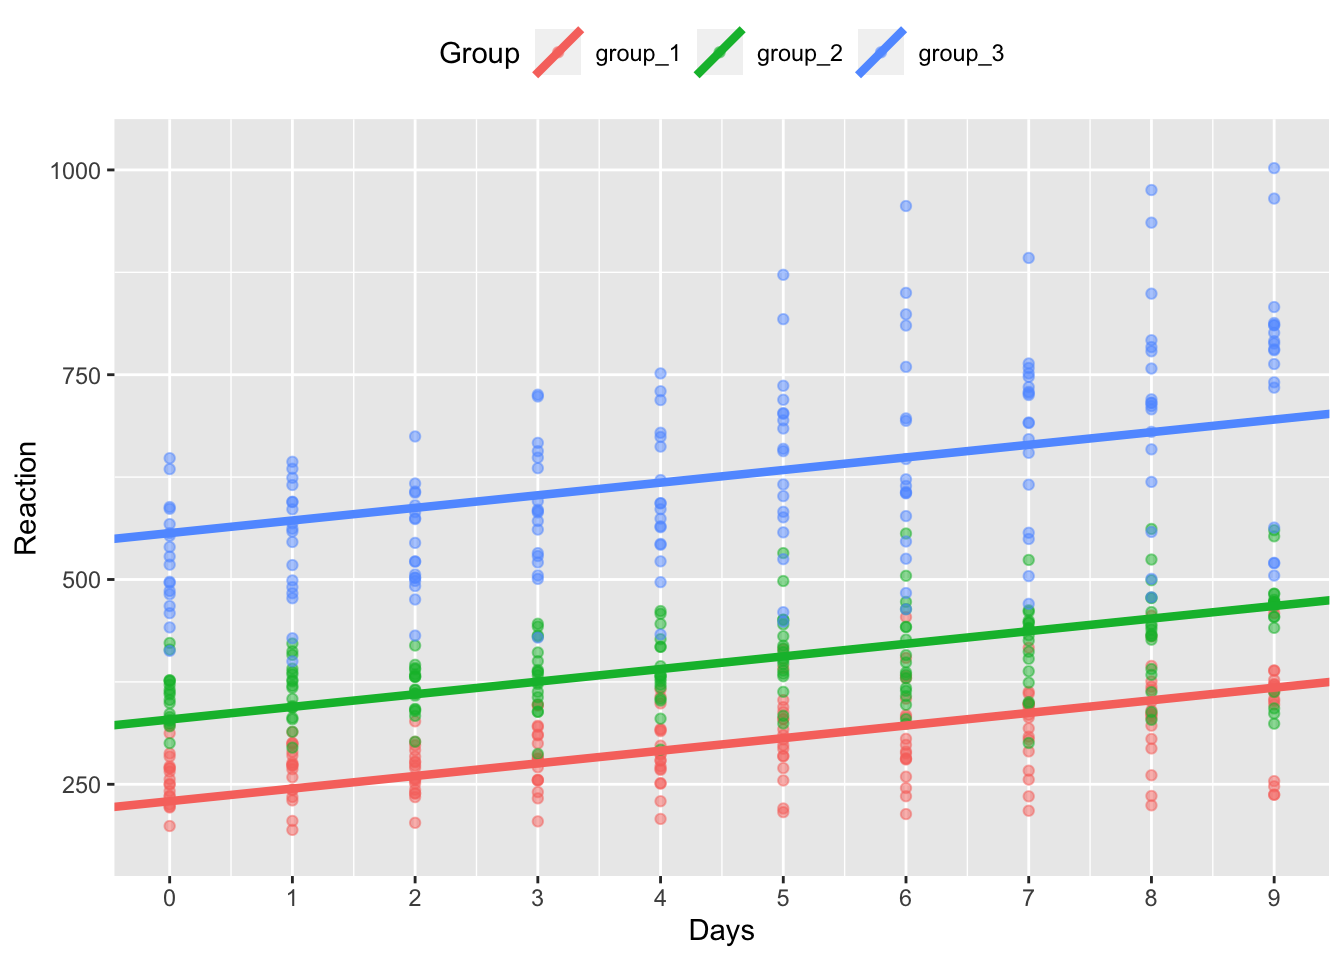
\includegraphics{r4psych_files/figure-latex/plot-random-intercepts-1.pdf}

Now you can see that we fit a model where the intercept (the y value at x = 0) differs across the 3 groups, but the slope of the lines is the same.

You might pick a random effects structure with random intercepts for data like this if you expect the three groups to differ from one another at the start of testing, but the effect of days on reaction times is the same across groups.

\hypertarget{random-slopes}{%
\subsubsection{Random Slopes}\label{random-slopes}}

Alternatively, we can specify a random effects structure with random slopes but fixed intercepts. We might pick this form if we expect all groups to start off at around the same score, but that the effects of days on reaction times differs across groups.

To specify this random effects structure, we change the 1 to a 0 in our random effects structure (specifying no or 0 random intercepts) and we put Days to the left of the \texttt{\textbar{}}, meaning that we want to calculate random slopes for the effect of Days for each Group.

\begin{Shaded}
\begin{Highlighting}[]
\CommentTok{\# fit random slopes model}
\NormalTok{model }\OtherTok{\textless{}{-}} \FunctionTok{lmer}\NormalTok{(Reaction }\SpecialCharTok{\textasciitilde{}}\NormalTok{ Days }\SpecialCharTok{+}\NormalTok{ (}\DecValTok{0} \SpecialCharTok{+}\NormalTok{ Days }\SpecialCharTok{|}\NormalTok{ Group), }\AttributeTok{data =}\NormalTok{ sleep\_groups)}

\CommentTok{\# see group coefficients}
\NormalTok{model\_coefs }\OtherTok{\textless{}{-}} \FunctionTok{coef}\NormalTok{(model)}\SpecialCharTok{$}\NormalTok{Group }\SpecialCharTok{\%\textgreater{}\%} 
  \FunctionTok{rename}\NormalTok{(}\AttributeTok{Intercept =} \StringTok{\textasciigrave{}}\AttributeTok{(Intercept)}\StringTok{\textasciigrave{}}\NormalTok{, }\AttributeTok{Slope =}\NormalTok{ Days) }\SpecialCharTok{\%\textgreater{}\%} 
  \FunctionTok{rownames\_to\_column}\NormalTok{(}\StringTok{"Group"}\NormalTok{)}

\CommentTok{\# see coefficients}
\NormalTok{model\_coefs}
\end{Highlighting}
\end{Shaded}

\begin{verbatim}
##     Group Intercept     Slope
## 1 group_1  371.6912 -8.479087
## 2 group_2  371.6912  7.249332
## 3 group_3  371.6912 47.441298
\end{verbatim}

Next, we'll join these coefficients to our original data.

\begin{Shaded}
\begin{Highlighting}[]
\NormalTok{sleep\_groups\_rans }\OtherTok{\textless{}{-}} \FunctionTok{left\_join}\NormalTok{(sleep\_groups, model\_coefs, }\AttributeTok{by =} \StringTok{"Group"}\NormalTok{)}
\end{Highlighting}
\end{Shaded}

Then we'll plot our original data with our new, random intercepts model. Here, we'll use a new, cheat function from ggplot, \texttt{\%+\%} (read: add components). This takes a fitted plot from ggplot, and replaces the data from that plot with whatever comes to the right of the function.

\begin{Shaded}
\begin{Highlighting}[]
\NormalTok{model\_coef\_plot }\SpecialCharTok{\%+\%}\NormalTok{ sleep\_groups\_rans}
\end{Highlighting}
\end{Shaded}

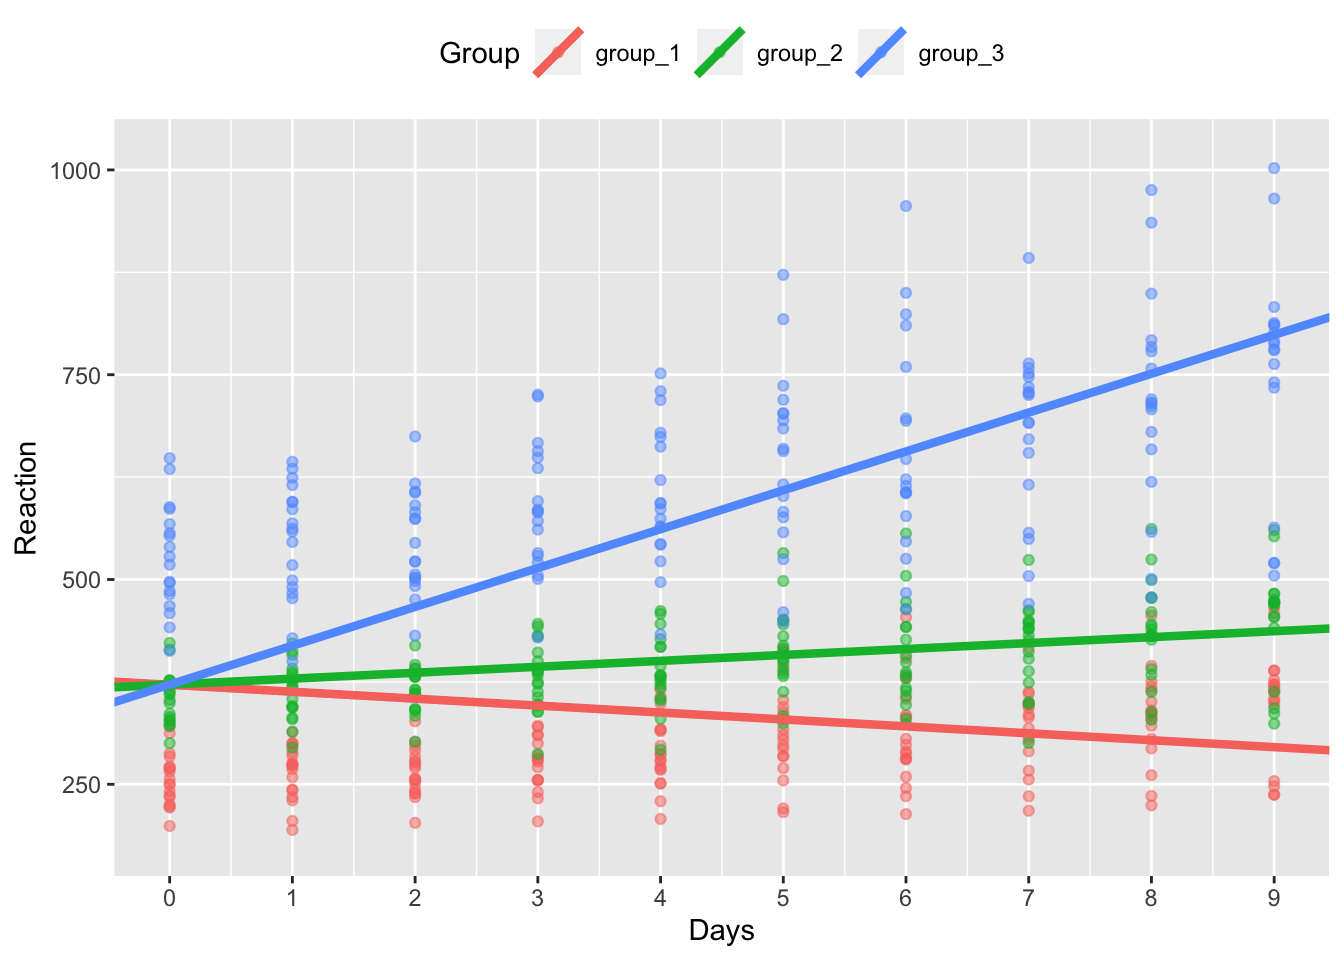
\includegraphics{r4psych_files/figure-latex/plot-random-slopes-1.pdf}

In the above plot, we can now see that our data has the same intercept across groups, but different slopes. It seems that the effect of days without sleep is greatest for group 3.

\hypertarget{random-intercepts-and-slopes}{%
\subsubsection{Random Intercepts and Slopes}\label{random-intercepts-and-slopes}}

Finally, we can specify that we want random intercepts and slopes for the group. Here, we just change the 0 back to a 1 in the random effects call.

\begin{Shaded}
\begin{Highlighting}[]
\CommentTok{\# fit random intercepts model}
\NormalTok{model }\OtherTok{\textless{}{-}} \FunctionTok{lmer}\NormalTok{(Reaction }\SpecialCharTok{\textasciitilde{}}\NormalTok{ Days }\SpecialCharTok{+}\NormalTok{ (}\DecValTok{1} \SpecialCharTok{+}\NormalTok{ Days }\SpecialCharTok{|}\NormalTok{ Group), }\AttributeTok{data =}\NormalTok{ sleep\_groups)}
\end{Highlighting}
\end{Shaded}

\begin{verbatim}
## Warning in checkConv(attr(opt, "derivs"), opt$par, ctrl = control$checkConv, :
## Model failed to converge with max|grad| = 0.00268565 (tol = 0.002, component 1)
\end{verbatim}

Let's see how these coefficients look.

\begin{Shaded}
\begin{Highlighting}[]
\CommentTok{\# see group coefficients}
\NormalTok{model\_coefs }\OtherTok{\textless{}{-}} \FunctionTok{coef}\NormalTok{(model)}\SpecialCharTok{$}\NormalTok{Group }\SpecialCharTok{\%\textgreater{}\%} 
  \FunctionTok{rename}\NormalTok{(}\AttributeTok{Intercept =} \StringTok{\textasciigrave{}}\AttributeTok{(Intercept)}\StringTok{\textasciigrave{}}\NormalTok{, }\AttributeTok{Slope =}\NormalTok{ Days) }\SpecialCharTok{\%\textgreater{}\%} 
  \FunctionTok{rownames\_to\_column}\NormalTok{(}\StringTok{"Group"}\NormalTok{)}

\CommentTok{\# see coefficients}
\NormalTok{model\_coefs}
\end{Highlighting}
\end{Shaded}

\begin{verbatim}
##     Group Intercept     Slope
## 1 group_1  256.4951  9.457048
## 2 group_2  344.2963 11.894270
## 3 group_3  514.2821 24.860226
\end{verbatim}

Next, we'll join these coefficients to our original data.

\begin{Shaded}
\begin{Highlighting}[]
\NormalTok{sleep\_groups\_ranis }\OtherTok{\textless{}{-}} \FunctionTok{left\_join}\NormalTok{(sleep\_groups, model\_coefs, }\AttributeTok{by =} \StringTok{"Group"}\NormalTok{)}
\end{Highlighting}
\end{Shaded}

Then we'll plot our original data with our new, random intercepts and random slopes model.

\begin{Shaded}
\begin{Highlighting}[]
\NormalTok{model\_coef\_plot }\SpecialCharTok{\%+\%}\NormalTok{ sleep\_groups\_ranis}
\end{Highlighting}
\end{Shaded}

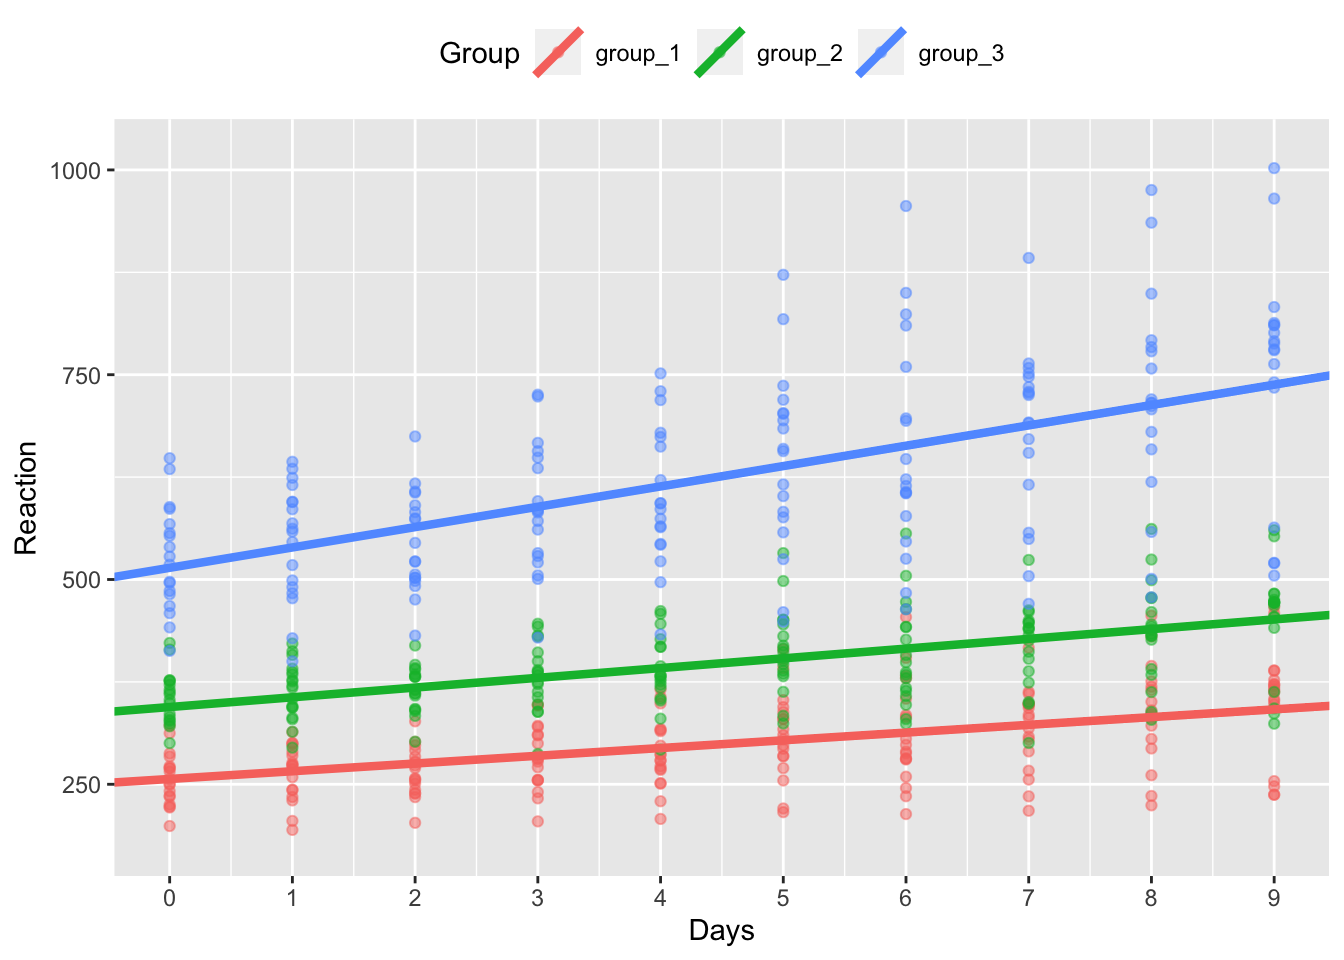
\includegraphics{r4psych_files/figure-latex/plot-random-intercepts-and-slopes-1.pdf}

As you can see, our model now fits random intercepts and slopes for each group of our participants.

\hypertarget{specifying-your-random-effects-structure}{%
\subsection{Specifying your Random Effects Structure}\label{specifying-your-random-effects-structure}}

There's some debate on how to specify your random effects, but one good rule of thumb is to \href{https://www.sciencedirect.com/science/article/pii/S0749596X12001180}{keep it maximal}. From several simulations, Dale Barr and colleagues have found that models that use the maximal random effects structure justified by the design of the study tend to have a good balance between power and type-I error rates (specifically keeping error below the nominal \(\alpha\)).

What does a maximal random effect structure look like? Typically, it will fit random intercepts, slopes, and the correlation between the two for any main effects and interactions in the model.

\href{https://www.sciencedirect.com/science/article/pii/S0749596X17300013}{Not all researchers agree that this is always the best choice}. Indeed, some argue that you should evaluate the goodness of fit for models with and without more complex terms in the model (such as random slopes and interactions) in order to get the best trade off between power and type-I error rates, especially at smaller sample sizes, and that maximal models inflate type-II error rates. The choice is up to you, but be informed about the choice you make.

\hypertarget{crossed-and-nested-random-effects}{%
\subsubsection{Crossed and Nested Random Effects}\label{crossed-and-nested-random-effects}}

To understand how to define your random effects, we'll look at some more simulated data. For illustration purposes, we won't fit these models (we'd really need more data for that), but just pay attention to the structure of the models.

\hypertarget{crossed-random-effects}{%
\paragraph{Crossed Random Effects}\label{crossed-random-effects}}

The random effects structure that you take should reflect the reality of the data. If you have a design where observations can be assigned to more than one random effect simultaneously, then these random effects are said to be crossed.

This is often the case when you have a repeated measures design where participants provide multiple observations through responding to several items. In this instance, each observation comes from an individual subject on an individual item at the same time, making each observation a unique combination of these random factors. Hence, the random effects of subjects and items are said to be crossed.

For this example, our data could look like the following:

\begin{Shaded}
\begin{Highlighting}[]
\NormalTok{crossed\_data }\OtherTok{\textless{}{-}} \FunctionTok{tibble}\NormalTok{(}
  \AttributeTok{Subject =} \FunctionTok{rep}\NormalTok{(}\DecValTok{1}\SpecialCharTok{:}\DecValTok{2}\NormalTok{, }\DecValTok{5}\NormalTok{),}
  \AttributeTok{Item =} \FunctionTok{rep}\NormalTok{(}\DecValTok{1}\SpecialCharTok{:}\DecValTok{5}\NormalTok{, }\AttributeTok{each =} \DecValTok{2}\NormalTok{),}
  \AttributeTok{Condition =} \FunctionTok{c}\NormalTok{(}\FunctionTok{rep}\NormalTok{(}\FunctionTok{c}\NormalTok{(}\StringTok{"A"}\NormalTok{, }\StringTok{"B"}\NormalTok{), }\DecValTok{2}\NormalTok{), }\FunctionTok{rep}\NormalTok{(}\FunctionTok{c}\NormalTok{(}\StringTok{"B"}\NormalTok{, }\StringTok{"A"}\NormalTok{), }\DecValTok{3}\NormalTok{)),}
  \AttributeTok{Response =} \FunctionTok{rnorm}\NormalTok{(}\AttributeTok{n =} \DecValTok{10}\NormalTok{, }\AttributeTok{mean =} \DecValTok{100}\NormalTok{, }\AttributeTok{sd =} \DecValTok{10}\NormalTok{)}
\NormalTok{)}
\NormalTok{crossed\_data}
\end{Highlighting}
\end{Shaded}

\begin{verbatim}
## # A tibble: 10 x 4
##    Subject  Item Condition Response
##      <int> <int> <chr>        <dbl>
##  1       1     1 A             92.8
##  2       2     1 B             85.0
##  3       1     2 A            108. 
##  4       2     2 B            109. 
##  5       1     3 B            100. 
##  6       2     3 A            106. 
##  7       1     4 B             92.8
##  8       2     4 A            111. 
##  9       1     5 B            118. 
## 10       2     5 A            105.
\end{verbatim}

Here, both participants take part in both conditions (A or B), hence this is a within-subjects design (but note that this dummy set is not balanced; real designs should be where possible). The condition (A or B) is therefore within individual subjects and individual items, but items are not only associated with one subject. Hence, our random effects are crossed, and should look like this:

\begin{Shaded}
\begin{Highlighting}[]
\FunctionTok{lmer}\NormalTok{(Response }\SpecialCharTok{\textasciitilde{}}\NormalTok{ Condition }\SpecialCharTok{+}\NormalTok{ (}\DecValTok{1} \SpecialCharTok{|}\NormalTok{ Subject) }\SpecialCharTok{+}\NormalTok{ (}\DecValTok{1} \SpecialCharTok{|}\NormalTok{ Item), }\AttributeTok{data =}\NormalTok{ crossed\_data)}
\end{Highlighting}
\end{Shaded}

\hypertarget{nested-random-effects}{%
\paragraph{Nested Random Effects}\label{nested-random-effects}}

Sometimes we get cases when our data are not crossed. For example, if you're testing participants from separate classes in separate schools, then your data can be said to be nested. The data are nested because observations come from students, which are a part of a specific class, and a specific school. In this instance, you should construct your data to reflect this nesting, ending up with something like this:

\begin{Shaded}
\begin{Highlighting}[]
\NormalTok{nested\_data }\OtherTok{\textless{}{-}} \FunctionTok{tibble}\NormalTok{(}
  \AttributeTok{Student =} \FunctionTok{seq}\NormalTok{(}\DecValTok{1}\SpecialCharTok{:}\DecValTok{10}\NormalTok{),}
  \AttributeTok{Class =} \FunctionTok{rep}\NormalTok{(}\FunctionTok{seq}\NormalTok{(}\DecValTok{1}\SpecialCharTok{:}\DecValTok{5}\NormalTok{), }\DecValTok{2}\NormalTok{),}
  \AttributeTok{School =} \FunctionTok{c}\NormalTok{(}\FunctionTok{rep}\NormalTok{(}\DecValTok{1}\NormalTok{, }\DecValTok{5}\NormalTok{), }\FunctionTok{rep}\NormalTok{(}\DecValTok{2}\NormalTok{, }\DecValTok{5}\NormalTok{)),}
  \AttributeTok{Intervention =} \FunctionTok{rep}\NormalTok{(}\FunctionTok{c}\NormalTok{(}\StringTok{"yes"}\NormalTok{, }\StringTok{"no"}\NormalTok{), }\DecValTok{5}\NormalTok{),}
  \AttributeTok{Outcome =} \FunctionTok{rnorm}\NormalTok{(}\AttributeTok{n =} \DecValTok{10}\NormalTok{, }\AttributeTok{mean =} \DecValTok{200}\NormalTok{, }\AttributeTok{sd =} \DecValTok{20}\NormalTok{)}
\NormalTok{)}

\NormalTok{nested\_data}
\end{Highlighting}
\end{Shaded}

\begin{verbatim}
## # A tibble: 10 x 5
##    Student Class School Intervention Outcome
##      <int> <int>  <dbl> <chr>          <dbl>
##  1       1     1      1 yes             195.
##  2       2     2      1 no              191.
##  3       3     3      1 yes             184.
##  4       4     4      1 no              169.
##  5       5     5      1 yes             249.
##  6       6     1      2 no              232.
##  7       7     2      2 yes             224.
##  8       8     3      2 no              199.
##  9       9     4      2 yes             170.
## 10      10     5      2 no              171.
\end{verbatim}

As you can see, your data are structured so that you have individuals with an identifier (column) for the class that they're in and for the school that they're in. We then have a column indicating whether or not students received an intervention, and their outcome on some test.

As a result, class 1 in school 1 is different to class 1 in school 2. How do you tell R to treat the data such that classes are nested within schools? Or to account for the school and class effects for each participant? We use a formula like this:

\begin{Shaded}
\begin{Highlighting}[]
\FunctionTok{lmer}\NormalTok{(Outcome }\SpecialCharTok{\textasciitilde{}}\NormalTok{ Intervention }\SpecialCharTok{+}\NormalTok{ (}\DecValTok{1} \SpecialCharTok{|}\NormalTok{ School}\SpecialCharTok{/}\NormalTok{Class}\SpecialCharTok{/}\NormalTok{Student), }\AttributeTok{data =}\NormalTok{ nested\_data)}
\end{Highlighting}
\end{Shaded}

Here, our random effects structure defines random intercepts for students, adjusting for similarities for students within the same class and school.

It's sometimes hard to figure out if you have nested or crossed (i.e.~not nested) data, and you can help your thinking (and Rs functioning) by simply using unique class identifiers for your school and class combinations. We can make this by simply pasting the identifiers for the School and Class together.

\begin{Shaded}
\begin{Highlighting}[]
\NormalTok{nested\_data}\SpecialCharTok{$}\NormalTok{Class\_ID }\OtherTok{\textless{}{-}} \FunctionTok{paste}\NormalTok{(nested\_data}\SpecialCharTok{$}\NormalTok{School, nested\_data}\SpecialCharTok{$}\NormalTok{Class, }\AttributeTok{sep =} \StringTok{"\_"}\NormalTok{)}
\NormalTok{nested\_data}
\end{Highlighting}
\end{Shaded}

\begin{verbatim}
## # A tibble: 10 x 6
##    Student Class School Intervention Outcome Class_ID
##      <int> <int>  <dbl> <chr>          <dbl> <chr>   
##  1       1     1      1 yes             195. 1_1     
##  2       2     2      1 no              191. 1_2     
##  3       3     3      1 yes             184. 1_3     
##  4       4     4      1 no              169. 1_4     
##  5       5     5      1 yes             249. 1_5     
##  6       6     1      2 no              232. 2_1     
##  7       7     2      2 yes             224. 2_2     
##  8       8     3      2 no              199. 2_3     
##  9       9     4      2 yes             170. 2_4     
## 10      10     5      2 no              171. 2_5
\end{verbatim}

Now your results will be exactly the same if you use either of these two formulas:

\begin{Shaded}
\begin{Highlighting}[]
\FunctionTok{lmer}\NormalTok{(Outcome }\SpecialCharTok{\textasciitilde{}}\NormalTok{ Intervention }\SpecialCharTok{+}\NormalTok{ (}\DecValTok{1} \SpecialCharTok{|}\NormalTok{ School}\SpecialCharTok{/}\NormalTok{Class\_ID), }\AttributeTok{data =}\NormalTok{ nested\_data)}
\FunctionTok{lmer}\NormalTok{(Outcome }\SpecialCharTok{\textasciitilde{}}\NormalTok{ Intervention }\SpecialCharTok{+}\NormalTok{ (}\DecValTok{1} \SpecialCharTok{|}\NormalTok{ School) }\SpecialCharTok{+}\NormalTok{ (}\DecValTok{1} \SpecialCharTok{|}\NormalTok{ Class\_ID), }\AttributeTok{data =}\NormalTok{ nested\_data)}
\end{Highlighting}
\end{Shaded}

If you don't have unique identifiers, using this second structure will give you incorrect results as R will think that every class was in every school, which is not the case.

These random effects structures take the simplest form where we have random intercepts only. In most cases, it's best to fit a more complex model depending upon the data you have.

\hypertarget{exploring-different-random-effects-structres}{%
\subsubsection{Exploring Different Random Effects Structres}\label{exploring-different-random-effects-structres}}

Let's say we have a within subjects design, where participants see half of the items in our study in one condition, and half in another condition. Let's take the \texttt{crossed\_data} example from before.

\begin{Shaded}
\begin{Highlighting}[]
\NormalTok{crossed\_data}
\end{Highlighting}
\end{Shaded}

\begin{verbatim}
## # A tibble: 10 x 4
##    Subject  Item Condition Response
##      <int> <int> <chr>        <dbl>
##  1       1     1 A             92.8
##  2       2     1 B             85.0
##  3       1     2 A            108. 
##  4       2     2 B            109. 
##  5       1     3 B            100. 
##  6       2     3 A            106. 
##  7       1     4 B             92.8
##  8       2     4 A            111. 
##  9       1     5 B            118. 
## 10       2     5 A            105.
\end{verbatim}

Here, we could fit random intercepts and slopes for subjects and items by adding condition (our slope term, or change in response for changes in 1 unit of condition) to the left of each term (along with the random intercept).

\begin{Shaded}
\begin{Highlighting}[]
\FunctionTok{lmer}\NormalTok{(Outcome }\SpecialCharTok{\textasciitilde{}}\NormalTok{ Condition }\SpecialCharTok{+}\NormalTok{ (}\DecValTok{1} \SpecialCharTok{+}\NormalTok{ Condition }\SpecialCharTok{|}\NormalTok{ Subject) }\SpecialCharTok{+}\NormalTok{ (}\DecValTok{1} \SpecialCharTok{+}\NormalTok{ Condition }\SpecialCharTok{|}\NormalTok{ Item), }\AttributeTok{data =}\NormalTok{ data)}
\end{Highlighting}
\end{Shaded}

What if participants take part in several blocks of this study? We might expect that their performance will improve from block to block. Here, we'd just have to add a fixed effect of study block and random effects on any factors that are affected by the blocking. If you repeat your items across blocks with the same subjects, you'd have random effects of block on subjects and items (along with condition). If you have new items in each block, you'd only have random slopes of block for subjects. These random effects structures look like this:

\begin{Shaded}
\begin{Highlighting}[]
\CommentTok{\# same items within each block}
\FunctionTok{lmer}\NormalTok{(}
\NormalTok{  Outcome }\SpecialCharTok{\textasciitilde{}}\NormalTok{ Condition }\SpecialCharTok{+}\NormalTok{ Block }\SpecialCharTok{+} 
\NormalTok{    (}\DecValTok{1} \SpecialCharTok{+}\NormalTok{ Condition }\SpecialCharTok{+}\NormalTok{ Block }\SpecialCharTok{|}\NormalTok{ Subject) }\SpecialCharTok{+} 
\NormalTok{    (}\DecValTok{1} \SpecialCharTok{+}\NormalTok{ Condition }\SpecialCharTok{+}\NormalTok{ Block }\SpecialCharTok{|}\NormalTok{ Item), }
  \AttributeTok{data =}\NormalTok{ data}
\NormalTok{  )}

\CommentTok{\# new items within each block}
\FunctionTok{lmer}\NormalTok{(}
\NormalTok{  Outcome }\SpecialCharTok{\textasciitilde{}}\NormalTok{ Condition }\SpecialCharTok{+}\NormalTok{ Block }\SpecialCharTok{+} 
\NormalTok{    (}\DecValTok{1} \SpecialCharTok{+}\NormalTok{ Condition }\SpecialCharTok{+}\NormalTok{ Block }\SpecialCharTok{|}\NormalTok{ Subject) }\SpecialCharTok{+} 
\NormalTok{    (}\DecValTok{1} \SpecialCharTok{+}\NormalTok{ Condition }\SpecialCharTok{|}\NormalTok{ Item), }
  \AttributeTok{data =}\NormalTok{ data}
\NormalTok{  )}
\end{Highlighting}
\end{Shaded}

As you might have guessed, for any between subjects factors, we cannot have a random slope of condition for that factor for each subject as subjects only see one condition. Here, our model might look like this:

\begin{Shaded}
\begin{Highlighting}[]
\FunctionTok{lmer}\NormalTok{(}
\NormalTok{  Outcome }\SpecialCharTok{\textasciitilde{}}\NormalTok{ Condition }\SpecialCharTok{+} 
\NormalTok{    (}\DecValTok{1} \SpecialCharTok{|}\NormalTok{ Subject) }\SpecialCharTok{+} 
\NormalTok{    (}\DecValTok{1} \SpecialCharTok{+}\NormalTok{ Condition }\SpecialCharTok{|}\NormalTok{ Item), }
  \AttributeTok{data =}\NormalTok{ data}
\NormalTok{  )}
\end{Highlighting}
\end{Shaded}

Where we can have random slopes for condition by item (as all items presumably see all conditions), but only random intercepts for subjects as they only see one condition.

Finally, as with all linear models, if we want an interaction between factors, we simply use an asterisk between factors to define our interactions, or a colon if we only want the interaction term and not main effects. This could take the form below if we want random intercepts and slopes for both factors on subjects and items, with main effects and interactions on our fixed factors.

\begin{Shaded}
\begin{Highlighting}[]
\FunctionTok{lmer}\NormalTok{(}
\NormalTok{  Outcome }\SpecialCharTok{\textasciitilde{}}\NormalTok{ factor\_A }\SpecialCharTok{*}\NormalTok{ factor\_B }\SpecialCharTok{+} 
\NormalTok{    (}\DecValTok{1} \SpecialCharTok{+}\NormalTok{ factor\_A }\SpecialCharTok{*}\NormalTok{ factor\_B }\SpecialCharTok{|}\NormalTok{ Subject) }\SpecialCharTok{+} 
\NormalTok{    (}\DecValTok{1} \SpecialCharTok{+}\NormalTok{ factor\_A }\SpecialCharTok{*}\NormalTok{ factor\_B }\SpecialCharTok{|}\NormalTok{ Item), }
  \AttributeTok{data =}\NormalTok{ data}
\NormalTok{  )}
\end{Highlighting}
\end{Shaded}

If you'd like to find out more about different structures, \href{http://rpsychologist.com/r-guide-longitudinal-lme-lmer}{Kristoffer Magnusson has a great guide} on this.

\hypertarget{partial-pooling-of-data}{%
\subsection{Partial-Pooling of Data}\label{partial-pooling-of-data}}

Here, we'll follow the first part of \href{https://tjmahr.github.io/plotting-partial-pooling-in-mixed-effects-models/}{TJ Mahr's excellent write up} of partial-pooling, and why this is so important for mixed effects models. Additionally, we'll see how partial-pooling allows mixed effects models to account for missing data.

We'll use the same data set as in TJ's article, the \texttt{sleepstudy} data set from the \texttt{lme4} package. I've already made some changes to this data set by convering it to a tibble and adding a few participants with missing data at the end by simulating new values based on the old participants, and simply deleting a few cells. Load the .csv file from the lesson materials folder to take a look at the data.

\begin{Shaded}
\begin{Highlighting}[]
\NormalTok{sleep\_study }\OtherTok{\textless{}{-}} \FunctionTok{read\_csv}\NormalTok{(}\StringTok{"inputs/sleep\_study\_with\_sim.csv"}\NormalTok{)}
\end{Highlighting}
\end{Shaded}

\begin{verbatim}
## Rows: 210 Columns: 3
## -- Column specification ------------------------------------
## Delimiter: ","
## dbl (3): Subject, Days, Reaction
## 
## i Use `spec()` to retrieve the full column specification for this data.
## i Specify the column types or set `show_col_types = FALSE` to quiet this message.
\end{verbatim}

First off, we'll fit a linear model to the data using complete pooling. This means that all of our data from each participant is put together to come up with one mean intercept and slope which is the same across all participants.

\begin{Shaded}
\begin{Highlighting}[]
\CommentTok{\# fit model}
\NormalTok{complete\_pooling }\OtherTok{\textless{}{-}} \FunctionTok{lm}\NormalTok{(Reaction }\SpecialCharTok{\textasciitilde{}}\NormalTok{ Days, }\AttributeTok{data =}\NormalTok{ sleep\_study)}

\CommentTok{\# tidy up and print model coefficients}
\NormalTok{complete\_pooling\_coefs }\OtherTok{\textless{}{-}} \FunctionTok{coef}\NormalTok{(complete\_pooling)}
\NormalTok{complete\_pooling\_coefs}
\end{Highlighting}
\end{Shaded}

\begin{verbatim}
## (Intercept)        Days 
##   252.09397    10.03451
\end{verbatim}

Next, we'll fit this model against our mean scores (with standard errors), observing how an increase in the days without sleep decreases reaction time.

\begin{Shaded}
\begin{Highlighting}[]
\FunctionTok{ggplot}\NormalTok{(}\AttributeTok{data =}\NormalTok{ sleep\_study, }\AttributeTok{mapping =} \FunctionTok{aes}\NormalTok{(}\AttributeTok{x =}\NormalTok{ Days, }\AttributeTok{y =}\NormalTok{ Reaction)) }\SpecialCharTok{+}
  \FunctionTok{geom\_abline}\NormalTok{(}\FunctionTok{aes}\NormalTok{(}\AttributeTok{intercept =}\NormalTok{ complete\_pooling\_coefs[}\DecValTok{1}\NormalTok{], }
                  \AttributeTok{slope =}\NormalTok{ complete\_pooling\_coefs[}\DecValTok{2}\NormalTok{]}
\NormalTok{                  ),}
              \AttributeTok{colour =} \StringTok{"\#F8766D"}\NormalTok{,}
              \AttributeTok{size =} \FloatTok{1.5}
\NormalTok{              ) }\SpecialCharTok{+}
  \FunctionTok{stat\_summary}\NormalTok{(}\AttributeTok{fun.data =} \StringTok{"mean\_se"}\NormalTok{, }
               \AttributeTok{geom =} \StringTok{"pointrange"}\NormalTok{,}
               \AttributeTok{na.rm =}\NormalTok{ T,}
               \AttributeTok{colour =} \StringTok{"\#F8766D"}\NormalTok{)}
\end{Highlighting}
\end{Shaded}

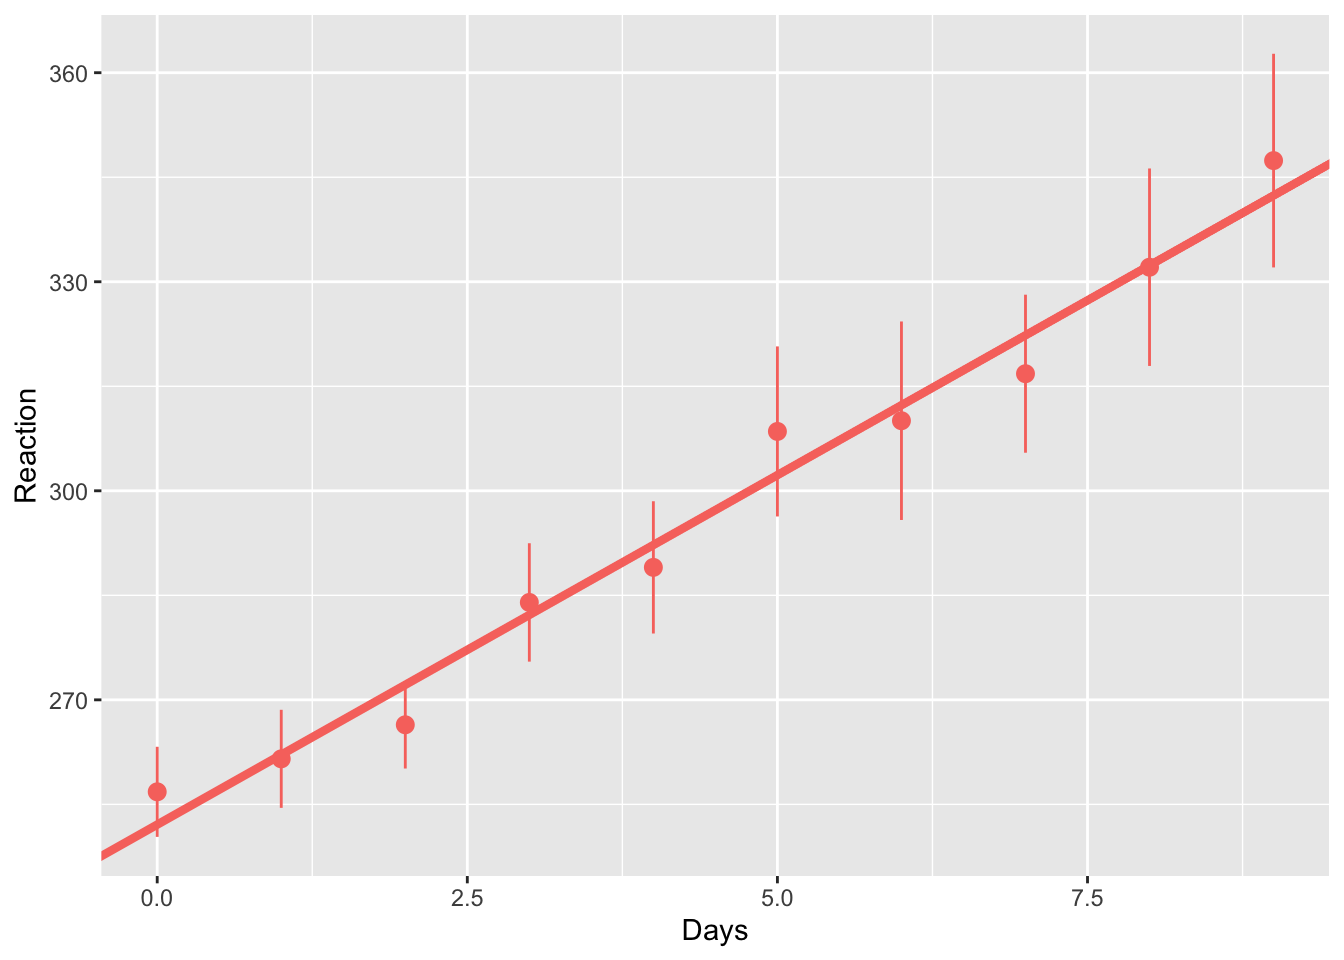
\includegraphics{r4psych_files/figure-latex/plot-complete-pooling-1.pdf}

You can see that this line fits the mean scores pretty well. But how does the data look at the individual level? Again, we'll save this plot as an object so we can update it later on. We'll also join these coefficients with our data so that we can easily update our plot when we explore different pooling choices.

\begin{Shaded}
\begin{Highlighting}[]
\NormalTok{complete }\OtherTok{\textless{}{-}} \FunctionTok{tibble}\NormalTok{(}
  \AttributeTok{Subject =} \FunctionTok{seq}\NormalTok{(}\DecValTok{1}\SpecialCharTok{:}\DecValTok{21}\NormalTok{),}
  \AttributeTok{Intercept =}\NormalTok{ complete\_pooling\_coefs[[}\DecValTok{1}\NormalTok{]],}
  \AttributeTok{Slope =}\NormalTok{ complete\_pooling\_coefs[[}\DecValTok{2}\NormalTok{]],}
  \AttributeTok{Model =} \StringTok{"complete\_pooling"}
\NormalTok{  )}

\NormalTok{model\_coefs }\OtherTok{\textless{}{-}} \FunctionTok{left\_join}\NormalTok{(sleep\_study, complete, }\AttributeTok{by =} \StringTok{"Subject"}\NormalTok{)}
\end{Highlighting}
\end{Shaded}

Let's see how the data look with no pooling.

\begin{Shaded}
\begin{Highlighting}[]
\NormalTok{pooling\_plot }\OtherTok{\textless{}{-}} \FunctionTok{ggplot}\NormalTok{(}\AttributeTok{data =}\NormalTok{ model\_coefs, }
       \AttributeTok{mapping =} \FunctionTok{aes}\NormalTok{(}\AttributeTok{x =}\NormalTok{ Days, }
                     \AttributeTok{y =}\NormalTok{ Reaction, }
                     \AttributeTok{colour =}\NormalTok{ Model)}
\NormalTok{       ) }\SpecialCharTok{+}
  \FunctionTok{geom\_abline}\NormalTok{(}\FunctionTok{aes}\NormalTok{(}\AttributeTok{intercept =}\NormalTok{ Intercept, }
                  \AttributeTok{slope =}\NormalTok{ Slope,}
                  \AttributeTok{colour =}\NormalTok{ Model),}
              \AttributeTok{size =} \FloatTok{1.5}
\NormalTok{              ) }\SpecialCharTok{+}
  \FunctionTok{geom\_point}\NormalTok{(}\AttributeTok{na.rm =}\NormalTok{ T) }\SpecialCharTok{+}
  \FunctionTok{facet\_wrap}\NormalTok{(}\SpecialCharTok{\textasciitilde{}}\NormalTok{Subject)}

\CommentTok{\# see the plot}
\NormalTok{pooling\_plot}
\end{Highlighting}
\end{Shaded}

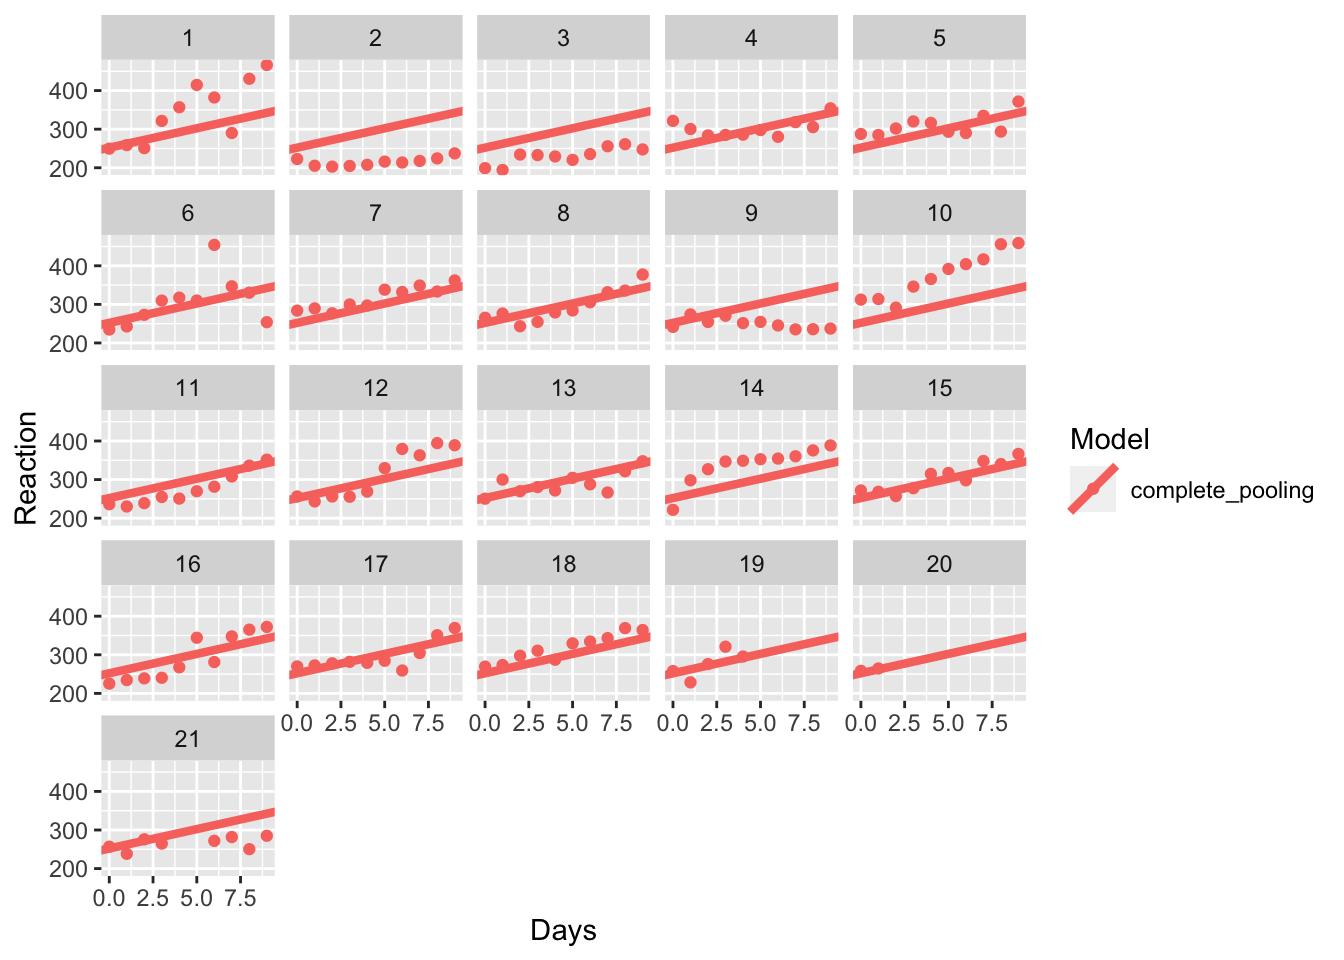
\includegraphics{r4psych_files/figure-latex/no-pooling-1.pdf}

Wow, so it looks like the model fits participant 18 very well. But what about participants 1, 2, and 14? Maybe a different model would fit their data better. It doesn't do a good job of explaining their responses, that's for sure!

One alternative to this complete pooling method is the opposite: no pooling. Here, we instead fit an individual intercepts and slopes to each individual in the data. We can do this by using the \texttt{lmer()} function from \textbf{lme4}. Here, our formula takes the form where reaction times are a function of the days (of deprived sleep) within each participant.

\begin{Shaded}
\begin{Highlighting}[]
\CommentTok{\# fit the model}
\NormalTok{no\_pooling }\OtherTok{\textless{}{-}} \FunctionTok{lmer}\NormalTok{(Reaction }\SpecialCharTok{\textasciitilde{}}\NormalTok{ Days }\SpecialCharTok{|}\NormalTok{ Subject, }\AttributeTok{data =}\NormalTok{ sleep\_study)}

\CommentTok{\# extract and view model coefficients}
\NormalTok{no\_pooling\_coefs }\OtherTok{\textless{}{-}} \FunctionTok{coef}\NormalTok{(no\_pooling)}\SpecialCharTok{$}\NormalTok{Subject }\SpecialCharTok{\%\textgreater{}\%} 
  \FunctionTok{rename}\NormalTok{(}\AttributeTok{Intercept =} \StringTok{\textasciigrave{}}\AttributeTok{(Intercept)}\StringTok{\textasciigrave{}}\NormalTok{, }\AttributeTok{Slope =}\NormalTok{ Days)}

\FunctionTok{head}\NormalTok{(no\_pooling\_coefs)}
\end{Highlighting}
\end{Shaded}

\begin{verbatim}
##         Slope Intercept
## 1 20.60380801  249.4076
## 2 -0.02559952  219.9904
## 3  3.66038038  219.0879
## 4  4.24609733  281.1159
## 5  6.27936095  278.4033
## 6  9.56692414  263.1531
\end{verbatim}

We can see for the first 6 participants their intercepts and slopes (Days) all differ from one another. How does this look in our plot? First, we'll add the two coefficients together for easy plotting.

\begin{Shaded}
\begin{Highlighting}[]
\NormalTok{none }\OtherTok{\textless{}{-}} \FunctionTok{tibble}\NormalTok{(}
  \AttributeTok{Subject =} \FunctionTok{seq}\NormalTok{(}\DecValTok{1}\SpecialCharTok{:}\DecValTok{21}\NormalTok{),}
  \AttributeTok{Intercept =}\NormalTok{ no\_pooling\_coefs}\SpecialCharTok{$}\NormalTok{Intercept,}
  \AttributeTok{Slope =}\NormalTok{ no\_pooling\_coefs}\SpecialCharTok{$}\NormalTok{Slope,}
  \AttributeTok{Model =} \StringTok{"no\_pooling"}
\NormalTok{)}
\NormalTok{complete\_none }\OtherTok{\textless{}{-}} \FunctionTok{bind\_rows}\NormalTok{(complete, none)}
\NormalTok{model\_coefs }\OtherTok{\textless{}{-}} \FunctionTok{left\_join}\NormalTok{(sleep\_study, complete\_none, }\AttributeTok{by =} \StringTok{"Subject"}\NormalTok{)}
\end{Highlighting}
\end{Shaded}

Now we've got our data in the correct format for plotting, we can have a look at how our models fit our data. Which do you think best matches the individual? Is this model any good when we have a lot of missing data?

Take a look at participant 20. Do you think the no pooling model is any better than the complete pooling model? What about participant 2?

\begin{Shaded}
\begin{Highlighting}[]
\NormalTok{pooling\_plot }\SpecialCharTok{\%+\%}\NormalTok{ model\_coefs}
\end{Highlighting}
\end{Shaded}

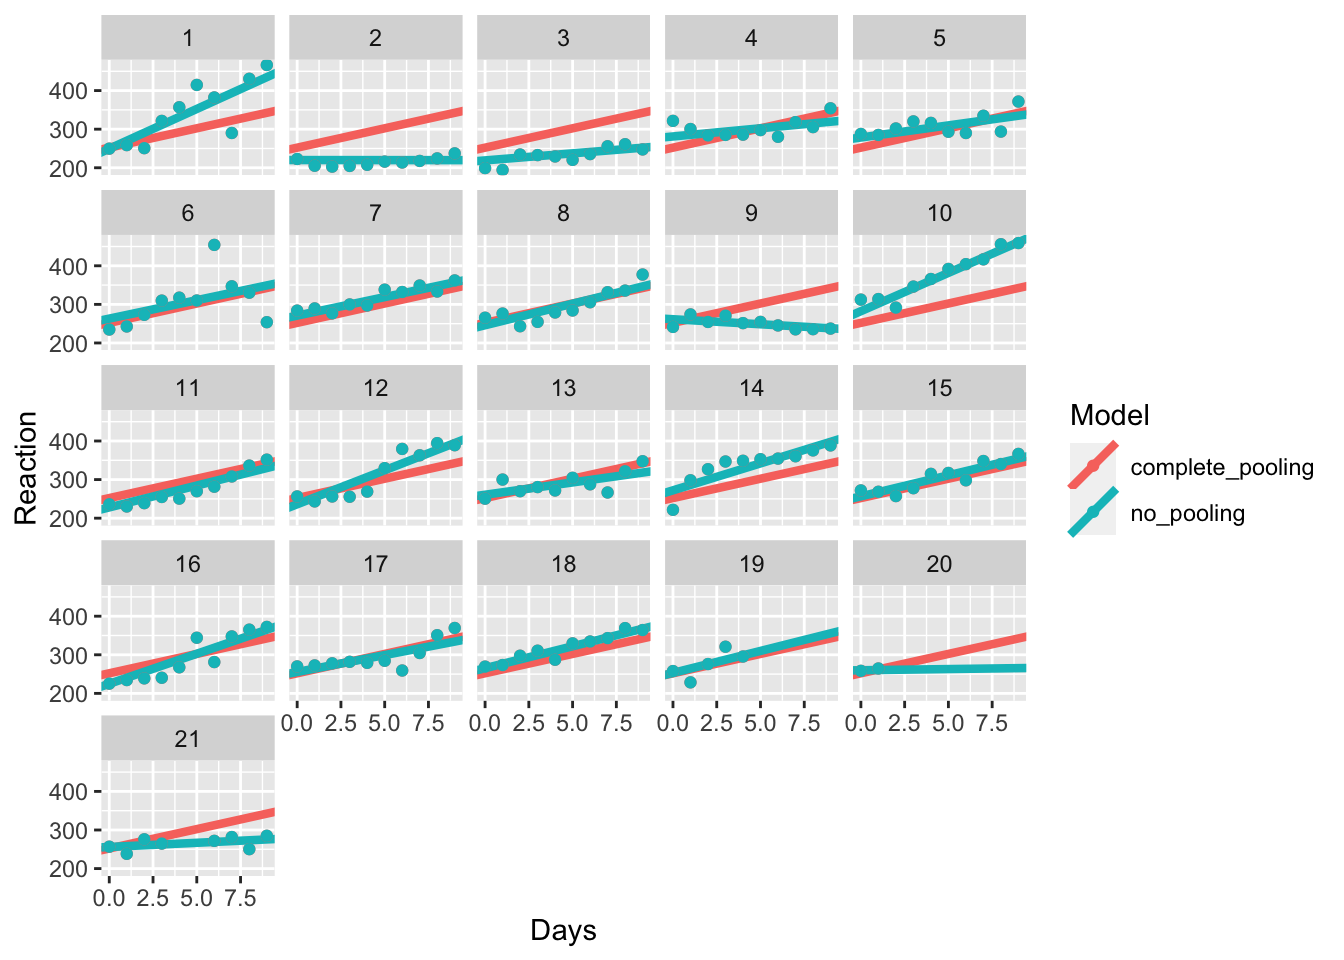
\includegraphics{r4psych_files/figure-latex/plot-pooling-no-pooling-1.pdf}

Finally, we get to where \textbf{lme4} shines; partial pooling of results. Here, we'll fit a mixed effects model where we have fixed effects of Days, which are assumed to be

\begin{Shaded}
\begin{Highlighting}[]
\NormalTok{partial\_pooling }\OtherTok{\textless{}{-}} \FunctionTok{lmer}\NormalTok{(Reaction }\SpecialCharTok{\textasciitilde{}}\NormalTok{ Days }\SpecialCharTok{+}\NormalTok{ (Days }\SpecialCharTok{|}\NormalTok{ Subject), }\AttributeTok{data =}\NormalTok{ sleep\_study)}
\end{Highlighting}
\end{Shaded}

\begin{Shaded}
\begin{Highlighting}[]
\CommentTok{\# extract model coefficients}
\NormalTok{partial\_pooling\_coefs }\OtherTok{\textless{}{-}} \FunctionTok{coef}\NormalTok{(partial\_pooling)}\SpecialCharTok{$}\NormalTok{Subject}

\CommentTok{\# make a tibble for partial pooling}
\NormalTok{partial }\OtherTok{\textless{}{-}} \FunctionTok{tibble}\NormalTok{(}
  \AttributeTok{Subject =} \FunctionTok{seq}\NormalTok{(}\DecValTok{1}\SpecialCharTok{:}\DecValTok{21}\NormalTok{),}
  \AttributeTok{Intercept =}\NormalTok{ partial\_pooling\_coefs}\SpecialCharTok{$}\StringTok{\textasciigrave{}}\AttributeTok{(Intercept)}\StringTok{\textasciigrave{}}\NormalTok{,}
  \AttributeTok{Slope =}\NormalTok{ partial\_pooling\_coefs}\SpecialCharTok{$}\NormalTok{Days,}
  \AttributeTok{Model =} \StringTok{"partial\_pooling"}
\NormalTok{)}

\CommentTok{\# clean up and combine with other models}
\NormalTok{partial }\OtherTok{\textless{}{-}}\NormalTok{ partial }\SpecialCharTok{\%\textgreater{}\%}
  \FunctionTok{left\_join}\NormalTok{(sleep\_study, }\AttributeTok{by =} \StringTok{"Subject"}\NormalTok{)}

\NormalTok{all\_pools }\OtherTok{\textless{}{-}} \FunctionTok{bind\_rows}\NormalTok{(model\_coefs, partial)}
\end{Highlighting}
\end{Shaded}

Next, we can plot the different models against one another to see what happens.

\begin{Shaded}
\begin{Highlighting}[]
\NormalTok{pooling\_plot }\SpecialCharTok{\%+\%}\NormalTok{ all\_pools}
\end{Highlighting}
\end{Shaded}

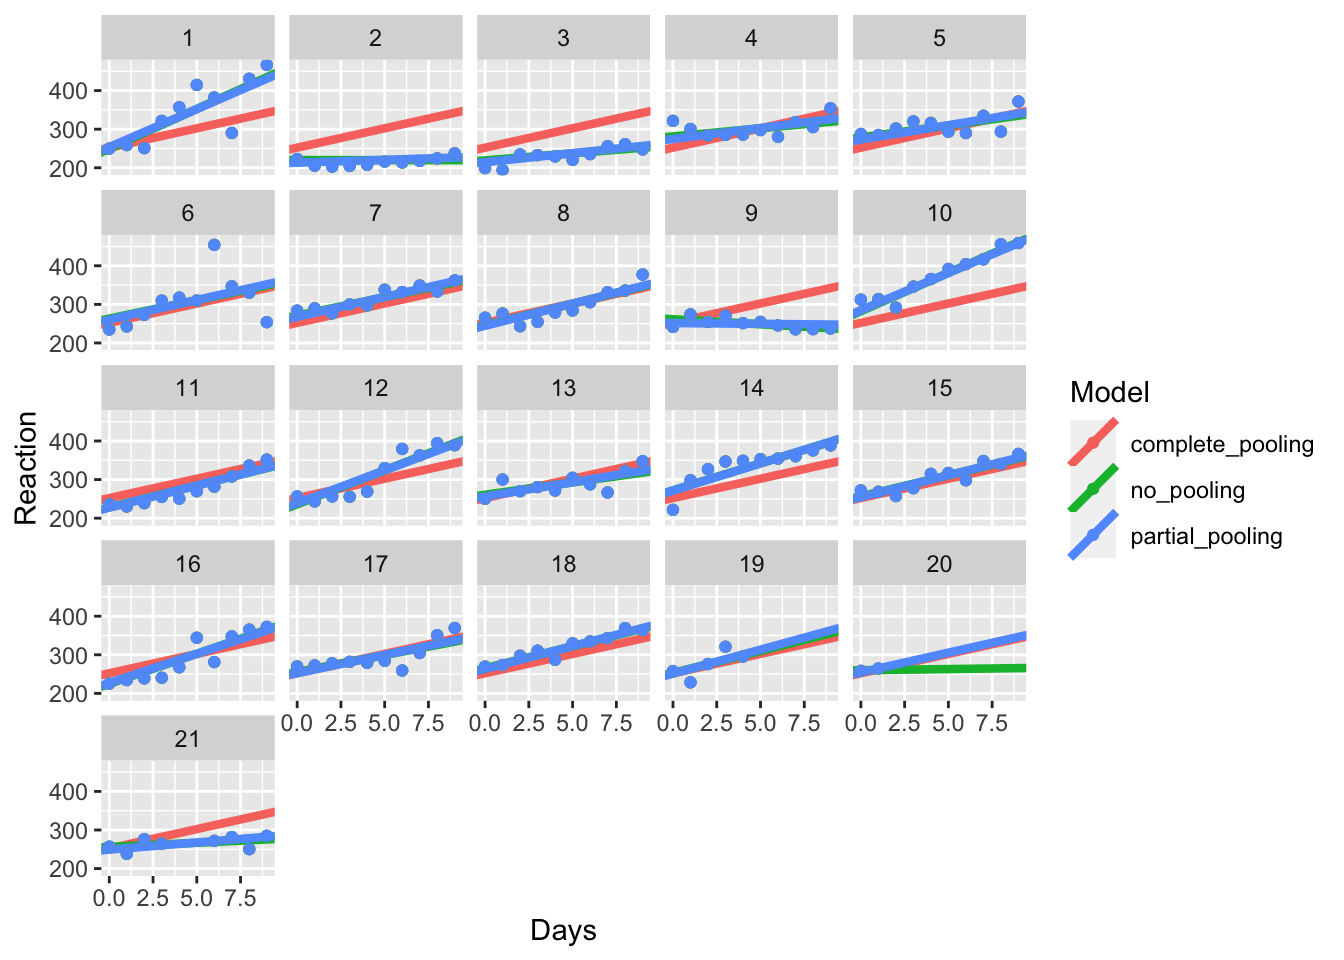
\includegraphics{r4psych_files/figure-latex/plot-partial-pooling-1.pdf}

As with TJ's article, we'll also zoom in to some of these participants too see what happens.

\begin{Shaded}
\begin{Highlighting}[]
\NormalTok{subset\_pools }\OtherTok{\textless{}{-}}\NormalTok{ all\_pools }\SpecialCharTok{\%\textgreater{}\%} \FunctionTok{filter}\NormalTok{(Subject }\SpecialCharTok{\%in\%} \FunctionTok{c}\NormalTok{(}\DecValTok{1}\NormalTok{, }\DecValTok{2}\NormalTok{, }\DecValTok{19}\NormalTok{, }\DecValTok{20}\NormalTok{))}
\NormalTok{pooling\_plot }\SpecialCharTok{\%+\%}\NormalTok{ subset\_pools}
\end{Highlighting}
\end{Shaded}

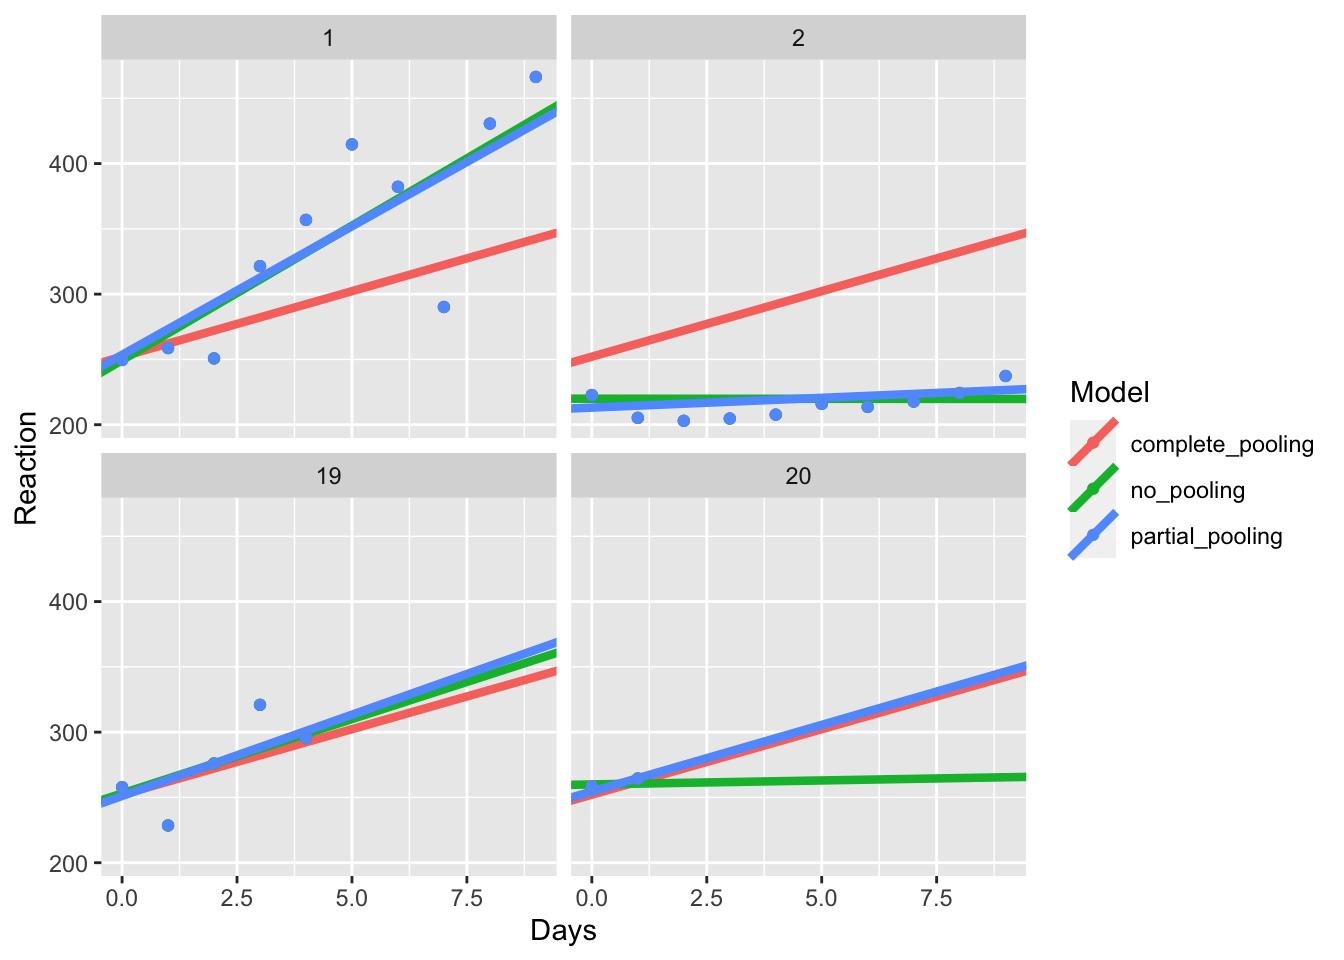
\includegraphics{r4psych_files/figure-latex/subset-partial-pooling-1.pdf}

Here, you can see that in the first two cases (1 and 2), the coefficients of the partial pooling model closely matches that of the no pooling model, showing that this model closely captures the individual differences within each participant.

Look at participant 20. You'll notice that the partial and complete pooling lines are more similar to one another. That's because while the partial pooling model fits individual intercepts and slopes for each participant, it is pulled towards the mean, i.e.~the overall intercept and slope across all participants. That's called shrinkage, where extreme values are pulled towards the average. This means that in cases where we have missing data, our model takes the best bet based on the grand mean, rather than trying to guess an individual intercept and slope based on that one person's data.

If you'd like to learn more about how this works, I really recommend consulting the source of this work, the article by \href{https://tjmahr.github.io/plotting-partial-pooling-in-mixed-effects-models/}{TJ Mahr on partial pooling}.

\hypertarget{interpreting-mixed-effects-model-output}{%
\section{Interpreting Mixed Effects Model Output}\label{interpreting-mixed-effects-model-output}}

Now that we've seen how mixed effects models work, we'll look at how to interpret the output of a mixed effects model. For this part, we'll use the \texttt{lexdec} dataset from the \texttt{languageR} library. Load this by loading the library and running the code below.

\begin{Shaded}
\begin{Highlighting}[]
\FunctionTok{library}\NormalTok{(languageR)}
\NormalTok{lex\_dec }\OtherTok{\textless{}{-}} \FunctionTok{as.tibble}\NormalTok{(lexdec) }\SpecialCharTok{\%\textgreater{}\%} 
  \FunctionTok{select}\NormalTok{(Subject, Trial, Word, NativeLanguage, RT)}
\end{Highlighting}
\end{Shaded}

In this data set, we have log transformed reaction times for English words rated by native and non-native speakers of English. Let's assume that we are interested in the influence of native language on reaction times. First, we want to set the intercept to the mean across both groups. Since the data isn't perfectly balanced, we should avoid the base \texttt{contrasts()} method from R, and instead centre our factors, so that one level is around -.5 and the other is .5. If your values aren't exactly -.5/.5, then your data set is unbalanced, so your should use this method.

\begin{Shaded}
\begin{Highlighting}[]
\CommentTok{\# centre the factor}
\NormalTok{lex\_dec}\SpecialCharTok{$}\NormalTok{lang\_c }\OtherTok{\textless{}{-}}\NormalTok{ (lex\_dec}\SpecialCharTok{$}\NormalTok{NativeLanguage }\SpecialCharTok{==} \StringTok{"English"}\NormalTok{) }\SpecialCharTok{{-}} \FunctionTok{mean}\NormalTok{(lex\_dec}\SpecialCharTok{$}\NormalTok{NativeLanguage }\SpecialCharTok{==} \StringTok{"English"}\NormalTok{)}

\CommentTok{\# see the result}
\FunctionTok{head}\NormalTok{(lex\_dec)}
\end{Highlighting}
\end{Shaded}

\begin{verbatim}
## # A tibble: 6 x 6
##   Subject Trial Word       NativeLanguage    RT lang_c
##   <fct>   <int> <fct>      <fct>          <dbl>  <dbl>
## 1 A1         23 owl        English         6.34  0.429
## 2 A1         27 mole       English         6.31  0.429
## 3 A1         29 cherry     English         6.35  0.429
## 4 A1         30 pear       English         6.19  0.429
## 5 A1         32 dog        English         6.03  0.429
## 6 A1         33 blackberry English         6.18  0.429
\end{verbatim}

Then we'll fit our model. We'll start out with a relatively simple model where we have crossed random effects with random intercepts by subjects (Subject) and items (Word). We'll then get a summary of our model to see what the \texttt{lmer} output looks like. We'll fit all models with ML since we're going to compare them to one another.

\begin{Shaded}
\begin{Highlighting}[]
\NormalTok{lexdec\_mod }\OtherTok{\textless{}{-}} \FunctionTok{lmer}\NormalTok{(RT }\SpecialCharTok{\textasciitilde{}}\NormalTok{ lang\_c }\SpecialCharTok{+}\NormalTok{ (}\DecValTok{1} \SpecialCharTok{|}\NormalTok{ Subject) }\SpecialCharTok{+}\NormalTok{ (}\DecValTok{1} \SpecialCharTok{|}\NormalTok{ Word), }\AttributeTok{data =}\NormalTok{ lex\_dec, }\AttributeTok{REML =}\NormalTok{ F)}
\FunctionTok{summary}\NormalTok{(lexdec\_mod)}
\end{Highlighting}
\end{Shaded}

\begin{verbatim}
## Linear mixed model fit by maximum likelihood  ['lmerMod']
## Formula: RT ~ lang_c + (1 | Subject) + (1 | Word)
##    Data: lex_dec
## 
##      AIC      BIC   logLik deviance df.resid 
##   -900.1   -873.0    455.1   -910.1     1654 
## 
## Scaled residuals: 
##     Min      1Q  Median      3Q     Max 
## -2.3600 -0.6142 -0.1196  0.4614  5.9658 
## 
## Random effects:
##  Groups   Name        Variance Std.Dev.
##  Word     (Intercept) 0.005896 0.07678 
##  Subject  (Intercept) 0.016741 0.12939 
##  Residual             0.029842 0.17275 
## Number of obs: 1659, groups:  Word, 79; Subject, 21
## 
## Fixed effects:
##             Estimate Std. Error t value
## (Intercept)  6.38509    0.02983 214.052
## lang_c      -0.15582    0.05769  -2.701
## 
## Correlation of Fixed Effects:
##        (Intr)
## lang_c 0.000
\end{verbatim}

There's a few things to unpack here. First, our model was fitted with \textbf{restricted maximum likelihood (REML)} rather than \textbf{maximum likelihood (ML)}. These are just different ways to estimate the parameters of the model. Andy Field (\citet{field2012discovering}) states that ML is typically better at estimating parameters for fixed regression parameters, and REML for random variances. The choice normally only makes a minor difference to the outcomes. However, we have to use ML if we want to compare model fits against one another.

Of most intereest to us are the random effects and fixed effects of the analysis. The random effects tells us how much variance in our data is captured by our random effects. Here, we can see that most of the variance is captured by the residuals (i.e.~unexplained variance), but including random intercepts for subjects and items goes some way to explaining the differences in scores. Here, means are always assumed to be 0, so we only get the variance and standard deviation for these terms.

Next, we have the fixed effects. These roughly correspond to the parameter estimates from regular linear models that we've looked at. As we can see, we have a \emph{t}-value of 2.57 for the effect of native language. The negative sign indicates that response times are slower for non-native speakers compared to the grand mean.

Finally, we get a correlation of our fixed effects, this is not the degree to which our fixed effects are related to one another, but is used for constructing confidence ellipses. We typically don't use this in reporting our statistics.

\hypertarget{calculating-p-values-for-parameter-estimates}{%
\subsection{Calculating p-values for Parameter Estimates}\label{calculating-p-values-for-parameter-estimates}}

You may have noticed that \texttt{lme4} doesn't provide you with \emph{p}-values for your parameter estimates. That's because there's some discussion on whether or not we can accurately do so with mixed effects models, and also because the creators of lme4 would rather you use parameter estimates and their standard errors to infer the strenth of evidence for an effect.

We can easily calculate these using Kenward-Roger or Satterthwaite approximations, which are provided by the \textbf{lmerTest} and \textbf{afex} packages in R.

However, to avoid loading more packages, we can use the normal approximation to calculate \emph{p}-values. The reasoning here is that with higher degrees of freedom, the t distribution matches the z distribution. Thus, we can treat the t-value as a z-value, essentially assuming infinite degrees of freedom.

Here, we look up the \emph{p}-value that matches the absolute (non-signed) \emph{t}-value for our parameters in the normal distribution. Then we subtract that value from 1 to get the probability of a \emph{t}-value exceeding the one we have, and multiply that by 2 to get a two-tailed \emph{p}-value.

We'll first ensure we have the \texttt{broom.mixed} function loaded to tidy up our model results from \texttt{lme4}. This can be installed like all packages from CRAN using:

\begin{Shaded}
\begin{Highlighting}[]
\FunctionTok{install.packages}\NormalTok{(}\StringTok{"broom.mixed"}\NormalTok{) }\CommentTok{\# install broom.mixed}
\FunctionTok{library}\NormalTok{(broom.mixed) }\CommentTok{\# load broom.mixed}
\end{Highlighting}
\end{Shaded}

Then we can tidy up our \texttt{lme4} output and calculate \emph{p}-values using the normal approximation as follows:

\begin{Shaded}
\begin{Highlighting}[]
\NormalTok{lexdec\_mod }\SpecialCharTok{\%\textgreater{}\%} 
  \FunctionTok{tidy}\NormalTok{(}\StringTok{"fixed"}\NormalTok{) }\SpecialCharTok{\%\textgreater{}\%} 
  \FunctionTok{mutate}\NormalTok{(}\AttributeTok{p\_value =} \DecValTok{2}\SpecialCharTok{*}\NormalTok{(}\DecValTok{1} \SpecialCharTok{{-}} \FunctionTok{pnorm}\NormalTok{(}\FunctionTok{abs}\NormalTok{(statistic))))}
\end{Highlighting}
\end{Shaded}

\begin{verbatim}
## # A tibble: 2 x 6
##   effect term        estimate std.error statistic p_value
##   <chr>  <chr>          <dbl>     <dbl>     <dbl>   <dbl>
## 1 fixed  (Intercept)    6.39     0.0298    214.   0      
## 2 fixed  lang_c        -0.156    0.0577     -2.70 0.00692
\end{verbatim}

Just be aware that this approach somewhat inflates type-I error rates (but only slightly so with large samples).

Another alternative we can use to assess whether we have a main effect of a factor with multiple levels is to use a model comparisons approach, which we'll look at next.

\hypertarget{model-selection}{%
\subsection{Model Selection}\label{model-selection}}

With the model comparisons approach, we simply fit our full model, and a model that is exactly the same as the full model, only without the fixed effect of interest. Here, because we want to check for a main effect of language, we simply fit a model with only an intercept term (and without an effect of language). Notice that the random effects stay the same.

\begin{Shaded}
\begin{Highlighting}[]
\NormalTok{lexdec\_mod\_reduced }\OtherTok{\textless{}{-}} \FunctionTok{lmer}\NormalTok{(RT }\SpecialCharTok{\textasciitilde{}} \DecValTok{1} \SpecialCharTok{+}\NormalTok{ (}\DecValTok{1} \SpecialCharTok{|}\NormalTok{ Subject) }\SpecialCharTok{+}\NormalTok{ (}\DecValTok{1} \SpecialCharTok{|}\NormalTok{ Word), }\AttributeTok{data =}\NormalTok{ lex\_dec, }\AttributeTok{REML =}\NormalTok{ F)}
\end{Highlighting}
\end{Shaded}

Then, we use the \texttt{anova()} function to check whether inclusion of the language fixed factor significantly improves model fit. Notice also that if we originally fit our models with REML, R will refit them with ML instead.

\begin{Shaded}
\begin{Highlighting}[]
\FunctionTok{anova}\NormalTok{(lexdec\_mod, lexdec\_mod\_reduced)}
\end{Highlighting}
\end{Shaded}

\begin{verbatim}
## Data: lex_dec
## Models:
## lexdec_mod_reduced: RT ~ 1 + (1 | Subject) + (1 | Word)
## lexdec_mod: RT ~ lang_c + (1 | Subject) + (1 | Word)
##                    npar     AIC     BIC logLik deviance  Chisq Df Pr(>Chisq)  
## lexdec_mod_reduced    4 -895.86 -874.20 451.93  -903.86                       
## lexdec_mod            5 -900.12 -873.05 455.06  -910.12 6.2605  1    0.01235 *
## ---
## Signif. codes:  0 '***' 0.001 '**' 0.01 '*' 0.05 '.' 0.1 ' ' 1
\end{verbatim}

Here, we're interested in the change in log-likelihood when we add terms to our model. Here, the increase in degrees of freedom should be one for each model you compare. We can see that adding the fixed effect of language significantly improved model fit, \(\chi^2(1) = 6.261, p = 0.012\). This means that we have a significant main effect of language.

We can similarly use this method to assess whether or not we should include random effects in our model, however whether or not you should select your random effects on the fly is again up for debate.

\begin{Shaded}
\begin{Highlighting}[]
\NormalTok{lexdec\_slope }\OtherTok{\textless{}{-}} \FunctionTok{lmer}\NormalTok{(RT }\SpecialCharTok{\textasciitilde{}}\NormalTok{ lang\_c }\SpecialCharTok{+}\NormalTok{ (}\DecValTok{1} \SpecialCharTok{|}\NormalTok{ Subject) }\SpecialCharTok{+}\NormalTok{ (lang\_c }\SpecialCharTok{||}\NormalTok{ Word), }\AttributeTok{data =}\NormalTok{ lex\_dec, }\AttributeTok{REML =}\NormalTok{ F)}
\NormalTok{lexdec\_slope\_cov }\OtherTok{\textless{}{-}} \FunctionTok{lmer}\NormalTok{(RT }\SpecialCharTok{\textasciitilde{}}\NormalTok{ lang\_c }\SpecialCharTok{+}\NormalTok{ (}\DecValTok{1} \SpecialCharTok{|}\NormalTok{ Subject) }\SpecialCharTok{+}\NormalTok{ (lang\_c }\SpecialCharTok{|}\NormalTok{ Word), }\AttributeTok{data =}\NormalTok{ lex\_dec, }\AttributeTok{REML =}\NormalTok{ F)}
\FunctionTok{anova}\NormalTok{(lexdec\_mod, lexdec\_slope, lexdec\_slope\_cov)}
\end{Highlighting}
\end{Shaded}

\begin{verbatim}
## Data: lex_dec
## Models:
## lexdec_mod: RT ~ lang_c + (1 | Subject) + (1 | Word)
## lexdec_slope: RT ~ lang_c + (1 | Subject) + ((1 | Word) + (0 + lang_c | Word))
## lexdec_slope_cov: RT ~ lang_c + (1 | Subject) + (lang_c | Word)
##                  npar     AIC     BIC logLik deviance   Chisq Df Pr(>Chisq)    
## lexdec_mod          5 -900.12 -873.05 455.06  -910.12                          
## lexdec_slope        6 -903.05 -870.57 457.53  -915.05  4.9348  1    0.02632 *  
## lexdec_slope_cov    7 -921.40 -883.51 467.70  -935.40 20.3514  1  6.445e-06 ***
## ---
## Signif. codes:  0 '***' 0.001 '**' 0.01 '*' 0.05 '.' 0.1 ' ' 1
\end{verbatim}

To understand what happened here, we need to look at our random effects. Look at the summary of the model with only random intercepts by subject and item. You can see that the random effects here are calculated for the intercept terms and for the residuals.

\begin{Shaded}
\begin{Highlighting}[]
\FunctionTok{summary}\NormalTok{(lexdec\_mod)}
\end{Highlighting}
\end{Shaded}

\begin{verbatim}
## Linear mixed model fit by maximum likelihood  ['lmerMod']
## Formula: RT ~ lang_c + (1 | Subject) + (1 | Word)
##    Data: lex_dec
## 
##      AIC      BIC   logLik deviance df.resid 
##   -900.1   -873.0    455.1   -910.1     1654 
## 
## Scaled residuals: 
##     Min      1Q  Median      3Q     Max 
## -2.3600 -0.6142 -0.1196  0.4614  5.9658 
## 
## Random effects:
##  Groups   Name        Variance Std.Dev.
##  Word     (Intercept) 0.005896 0.07678 
##  Subject  (Intercept) 0.016741 0.12939 
##  Residual             0.029842 0.17275 
## Number of obs: 1659, groups:  Word, 79; Subject, 21
## 
## Fixed effects:
##             Estimate Std. Error t value
## (Intercept)  6.38509    0.02983 214.052
## lang_c      -0.15582    0.05769  -2.701
## 
## Correlation of Fixed Effects:
##        (Intr)
## lang_c 0.000
\end{verbatim}

Look at the next model, with random slopes added. Here, we use the double pipe (\texttt{\textbar{}\textbar{}}) in our random effects to specify that we want random intercepts and slopes, but we don't want to calculate the intercept-slope covariance. (But, note that this only works for numeric, continuous predictors; centering again helps here.) This can be seen in our random effects where we have \texttt{Word\ lang\_c} which shows the slope for language by item, \texttt{Word.1\ (Intercept)} which is the intercept for items, and \texttt{Subject\ (Intercept)} which shows the intercept for the subjects.

\begin{Shaded}
\begin{Highlighting}[]
\FunctionTok{summary}\NormalTok{(lexdec\_slope)}
\end{Highlighting}
\end{Shaded}

\begin{verbatim}
## Linear mixed model fit by maximum likelihood  ['lmerMod']
## Formula: RT ~ lang_c + (1 | Subject) + ((1 | Word) + (0 + lang_c | Word))
##    Data: lex_dec
## 
##      AIC      BIC   logLik deviance df.resid 
##   -903.1   -870.6    457.5   -915.1     1653 
## 
## Scaled residuals: 
##     Min      1Q  Median      3Q     Max 
## -2.5314 -0.6105 -0.1222  0.4714  6.0190 
## 
## Random effects:
##  Groups   Name        Variance Std.Dev.
##  Word     lang_c      0.002351 0.04849 
##  Word.1   (Intercept) 0.005924 0.07697 
##  Subject  (Intercept) 0.016757 0.12945 
##  Residual             0.029237 0.17099 
## Number of obs: 1659, groups:  Word, 79; Subject, 21
## 
## Fixed effects:
##             Estimate Std. Error t value
## (Intercept)  6.38509    0.02984 213.959
## lang_c      -0.15582    0.05797  -2.688
## 
## Correlation of Fixed Effects:
##        (Intr)
## lang_c 0.000
\end{verbatim}

Finally, if we look at the more complex model, we can see that we have intercepts and slopes for the items, and we've calculated the covariance between these terms (in the \texttt{Corr} column.

\begin{Shaded}
\begin{Highlighting}[]
\FunctionTok{summary}\NormalTok{(lexdec\_slope\_cov)}
\end{Highlighting}
\end{Shaded}

\begin{verbatim}
## Linear mixed model fit by maximum likelihood  ['lmerMod']
## Formula: RT ~ lang_c + (1 | Subject) + (lang_c | Word)
##    Data: lex_dec
## 
##      AIC      BIC   logLik deviance df.resid 
##   -921.4   -883.5    467.7   -935.4     1652 
## 
## Scaled residuals: 
##     Min      1Q  Median      3Q     Max 
## -2.6132 -0.6175 -0.1112  0.4677  6.1894 
## 
## Random effects:
##  Groups   Name        Variance Std.Dev. Corr 
##  Word     (Intercept) 0.005924 0.07697       
##           lang_c      0.002349 0.04846  -0.98
##  Subject  (Intercept) 0.016757 0.12945       
##  Residual             0.029237 0.17099       
## Number of obs: 1659, groups:  Word, 79; Subject, 21
## 
## Fixed effects:
##             Estimate Std. Error t value
## (Intercept)  6.38509    0.02984 213.961
## lang_c      -0.15582    0.05797  -2.688
## 
## Correlation of Fixed Effects:
##        (Intr)
## lang_c -0.027
\end{verbatim}

It seems that this model better explains our data than the other models, so we should probably use this one. Still, the choice of random effects structure can be as much driven by your assumptions and knowledge of the source of the data as from these data driven techniques.

\hypertarget{failure-to-converge-what-should-i-do}{%
\subsection{Failure to Converge: What Should I Do?}\label{failure-to-converge-what-should-i-do}}

Often, when you attempt to fit the maximal random effects structure you will get an error saying that your model failed to converge. This means that you don't have enough information in your data (or your data is so noisy) that you cannot properly identify the full variance covariance matrix for the model. This happens a lot if you have variances that are equal or nearly equal to 0, or correlations in terms that are equal to -1 or 1.

One way to avoid problems with converging is to centre your factors (as we have done above) and use numeric predictors in your model. You can also try to use a different optimiser by specifying the options in \texttt{lme4}. You can specify your optimiser like so. Check out the summaries of these models to see how they differ. Basically, these optimisers are just different methods for attempting to find the best fitting model for your data.

\begin{Shaded}
\begin{Highlighting}[]
\NormalTok{nelder\_mod }\OtherTok{\textless{}{-}} \FunctionTok{lmer}\NormalTok{(}
\NormalTok{  RT }\SpecialCharTok{\textasciitilde{}}\NormalTok{ lang\_c }\SpecialCharTok{+}\NormalTok{ (}\DecValTok{1} \SpecialCharTok{|}\NormalTok{ Subject) }\SpecialCharTok{+}\NormalTok{ (lang\_c }\SpecialCharTok{|}\NormalTok{ Word), }
  \AttributeTok{data =}\NormalTok{ lex\_dec, }\AttributeTok{REML =}\NormalTok{ F, }
  \AttributeTok{control =} \FunctionTok{lmerControl}\NormalTok{(}\AttributeTok{optimizer =} \StringTok{"Nelder\_Mead"}\NormalTok{)}
\NormalTok{  )}
\NormalTok{boby\_mod }\OtherTok{\textless{}{-}} \FunctionTok{lmer}\NormalTok{(}
\NormalTok{  RT }\SpecialCharTok{\textasciitilde{}}\NormalTok{ lang\_c }\SpecialCharTok{+}\NormalTok{ (}\DecValTok{1} \SpecialCharTok{|}\NormalTok{ Subject) }\SpecialCharTok{+}\NormalTok{ (lang\_c }\SpecialCharTok{|}\NormalTok{ Word), }
  \AttributeTok{data =}\NormalTok{ lex\_dec, }\AttributeTok{REML =}\NormalTok{ F, }
  \AttributeTok{control =} \FunctionTok{lmerControl}\NormalTok{(}\AttributeTok{optimizer =} \StringTok{"bobyqa"}\NormalTok{)}
\NormalTok{     )}
\end{Highlighting}
\end{Shaded}

Also, if you have complex models, with intercepts and slopes calculated for subjects and items for something that is also a fixed effect, your model can effectively run out of the degrees of freedom to estimate the correlations between your intercepts and slopes. One work around here is to just simplify your model. There are a number of suggestions for how you should do this.

In psychological research, \href{https://hlplab.wordpress.com/2009/05/14/random-effect-structure/}{one suggested procedure} is as follows:

For a model specified as \texttt{lmer(outcome\ \textasciitilde{}\ A\ *\ B\ +\ (1\ +\ A\ *\ B\ \textbar{}\ subjects)\ +\ (1\ +\ A\ *\ B\ \textbar{}\ items),\ data)}:

\begin{itemize}
\tightlist
\item
  First remove the correlations between random effects, i.e.~\texttt{(1\ +\ A\ +\ B\ \textbar{}\ subjects)\ +\ (1\ +\ A\ +\ B\ \textbar{}\ items)}
\item
  If that doesn't converge, remove the by-items slopes for one factor (which explains the least variance) first. \texttt{(1\ +\ A\ +\ B\ \textbar{}\ subjects)\ +\ (1\ +\ A\ \textbar{}\ items)}
\item
  If that doesn't converge, remove the reamining by-items slopes \texttt{(1\ +\ A\ +\ B\ \textbar{}\ subjects)\ +\ (1\ \textbar{}\ items)}
\item
  Remove slopes on subjects until it eventually converges
\end{itemize}

The reasoning here is that in our experiments we attempt to control as many confounds in our items as possible, such that variance within items should be smaller than variance within subjects.

If your model doesn't converge with random intercepts by both terms, you should probably explore your data for potential problems.

\hypertarget{test-assumptions}{%
\section{Test Assumptions}\label{test-assumptions}}

While mixed effects models get around many of the stricter assumptions from linear models, these models still make some assumptions. Some assumptions you need to worry about include:

\begin{itemize}
\item
  Linearity: Unsurprisingly, linear models require linearly related data. You can check for this with a graph as in previous sections. Alternatively, you can fit a non-linear function to your model.
\item
  Independence: If your data are not independent (e.g.~with multiple responses per participant) then your model must specify this is the case through your random effects. Failing to do so will lead to violations of this assumption, and incorrectly fitted models.
\item
  Normal Distribution of Random Coefficients: random coefficients are assumed to be normally distributed around the model. For random intercepts models this means that your intercepts are supposed to be normally distributed around the overall model (\citet{field2012discovering}).
\item
  Multicollinearity: This is where one predictor in your model can be can be reasonably accurately linearly predicted from the other predictors in your model. You can check for this by using the \texttt{vif()} function from the \texttt{usdm} library. Centering your predictors can help with problems of multicollinearity.
\item
  Homoscedasticity: The error term in your model should be the same across all of your variables. You could use a Levene's test or a plot of residuals vs.~fitted values, as with regular linear models.
\item
  Outliers: Large outliers will skew your data. You can check for these using any traditional means, e.g.~eye-balling your data via graphs or excluding based on some reasonable criteria (e.g.~+ 3SD above the mean). Just make sure you have a principled decision for excluding data.
\end{itemize}

\hypertarget{generalised-mixed-effects-models}{%
\section{Generalised Mixed Effects Models}\label{generalised-mixed-effects-models}}

Generalised mixed effects models are performed in a similar way to mixed effects models, but are applied to cases when your outcome or dependent variable is not normally distributed, e.g.~logistic regression for binary response data. These models use the same logic as generalised linear models, and the interpretation is very similar to mixed effects models. However here the \emph{p}-values are calculated for the fixed effects coefficients straight out of the model!

We implement these models for binary response data like so:

\begin{Shaded}
\begin{Highlighting}[]
\FunctionTok{glmer}\NormalTok{(}
\NormalTok{  DV\_binom }\SpecialCharTok{\textasciitilde{}} \CommentTok{\# binomial dependent variable}
\NormalTok{    A }\SpecialCharTok{*}\NormalTok{ B }\SpecialCharTok{+} \CommentTok{\# fixed effects}
\NormalTok{    (A }\SpecialCharTok{*}\NormalTok{ B }\SpecialCharTok{|}\NormalTok{ subject) }\SpecialCharTok{+}\NormalTok{ (A }\SpecialCharTok{*}\NormalTok{ B }\SpecialCharTok{|}\NormalTok{ item), }\CommentTok{\# random effects }
  \AttributeTok{family =}\NormalTok{ binomial, }\CommentTok{\# family: type of distribution}
  \AttributeTok{data =}\NormalTok{ data, }
  \FunctionTok{glmerControl}\NormalTok{(}\AttributeTok{optimizer =} \StringTok{"bobyqa"}\NormalTok{) }\CommentTok{\# options; notice glmerControl (not lmer)}
\NormalTok{  )}
\end{Highlighting}
\end{Shaded}

For proportions, we simply set the weights of the model to the number of success and provide the proportions as our dependent variable.

\begin{Shaded}
\begin{Highlighting}[]
\FunctionTok{glmer}\NormalTok{(}
\NormalTok{  DV\_prop }\SpecialCharTok{\textasciitilde{}} \CommentTok{\# dependent variable as a proportion}
\NormalTok{    A }\SpecialCharTok{*}\NormalTok{ B }\SpecialCharTok{+} \CommentTok{\# fixed effects}
\NormalTok{    (A }\SpecialCharTok{*}\NormalTok{ B }\SpecialCharTok{|}\NormalTok{ subject) }\SpecialCharTok{+}\NormalTok{ (A }\SpecialCharTok{*}\NormalTok{ B }\SpecialCharTok{|}\NormalTok{ item), }\CommentTok{\# random effects }
  \AttributeTok{family =}\NormalTok{ binomial, }\CommentTok{\# family: type of distribution}
  \AttributeTok{weights =}\NormalTok{ N\_observations, }\CommentTok{\# number of observations making up the proportion}
  \AttributeTok{data =}\NormalTok{ data,}
  \FunctionTok{glmerControl}\NormalTok{(}\AttributeTok{optimizer =} \StringTok{"bobyqa"}\NormalTok{)}\CommentTok{\# options; notice glmerControl (not lmer)}
\NormalTok{  )}
\end{Highlighting}
\end{Shaded}

Alternatively, we can calculate these within the model if we have the number of successes and the number of observations as columns in our model.

\begin{Shaded}
\begin{Highlighting}[]
\FunctionTok{glmer}\NormalTok{(}
\NormalTok{  DV\_successes}\SpecialCharTok{/}\NormalTok{N\_observations }\SpecialCharTok{\textasciitilde{}} \CommentTok{\# calculate proportion}
\NormalTok{    A }\SpecialCharTok{*}\NormalTok{ B }\SpecialCharTok{+} \CommentTok{\# fixed effects}
\NormalTok{    (A }\SpecialCharTok{*}\NormalTok{ B }\SpecialCharTok{|}\NormalTok{ subject) }\SpecialCharTok{+}\NormalTok{ (A }\SpecialCharTok{*}\NormalTok{ B }\SpecialCharTok{|}\NormalTok{ item), }\CommentTok{\# random effects }
  \AttributeTok{family =}\NormalTok{ binomial, }\CommentTok{\# family: type of distribution}
  \AttributeTok{weights =}\NormalTok{ N\_observations, }\CommentTok{\# number of observations making up the proportion}
  \AttributeTok{data =}\NormalTok{ data,}
  \FunctionTok{glmerControl}\NormalTok{(}\AttributeTok{optimizer =} \StringTok{"bobyqa"}\NormalTok{) }\CommentTok{\# options; notice glmerControl (not lmer)}
\NormalTok{  )}
\end{Highlighting}
\end{Shaded}

Here, our parameter estimates are interpreted as log likelihoods.

\hypertarget{a-note-on-power-effect-sizes-and-pairwise-comparisons}{%
\section{A Note on Power, Effect Sizes, and Pairwise Comparisons}\label{a-note-on-power-effect-sizes-and-pairwise-comparisons}}

\hypertarget{power}{%
\subsection{Power}\label{power}}

Power analysis is rather complex for mixed effects models. Here, simulation is key, and there are some packages out there to help you perform your own power analyses with little coding, such as SIMR (\texttt{install.packages("simr")}). You can find a paper on \href{https://besjournals.onlinelibrary.wiley.com/doi/abs/10.1111/2041-210X.12504}{how to use SIMR here}.

\hypertarget{effect-sizes}{%
\subsection{Effect Sizes}\label{effect-sizes}}

Effect sizes for individual parameter estimates and/or the entire model fit are often not reported with mixed effects models due to the practical and/or technical difficulties posed by calculating effect sizes. However, there are some options out there, such as that offered by the \texttt{r2beta()} function from the \textbf{r2glmm package}, or the \texttt{r.squaredGLMM()} function from the \textbf{MuMIn package}. I'll leave it up to you to explore these options, but we might return to this in the final lesson.

\hypertarget{pairwise-comparisons}{%
\subsection{Pairwise Comparisons}\label{pairwise-comparisons}}

Pairwise comparisons can be conducted in the same way as for linear models. You can either subset your data to the a single level of one factor to explore the simple effects for another factor, adjusting your \emph{p}-values manually in the process, or you can use the \texttt{glht()} function from the \textbf{multcomp} package.

\hypertarget{exercises-8}{%
\section{Exercises}\label{exercises-8}}

For these exercises, we will look at the core concepts from this lesson. Here, we'll use a simulated data set that's saved as a .csv in the inputs folder.

If you don't have access to these, please \href{https://github.com/gpwilliams/r4psych}{download the repository from GitHub} and open the \textbf{lesson\_materials} folder. Open the relevant folder for this lesson. If you work out of the file \textbf{09\_mixed\_effects\_models.Rmd} the code below will work to load the data set. If this fails then quit R and open it up from the .Rmd file above so your working directory is in the correct folder.

\begin{Shaded}
\begin{Highlighting}[]
\FunctionTok{library}\NormalTok{(tidyverse)}
\FunctionTok{library}\NormalTok{(lme4)}
\end{Highlighting}
\end{Shaded}

\begin{Shaded}
\begin{Highlighting}[]
\NormalTok{dat }\OtherTok{\textless{}{-}} \FunctionTok{read\_csv}\NormalTok{(}\StringTok{"inputs/factorial\_data.csv"}\NormalTok{)}
\end{Highlighting}
\end{Shaded}

\hypertarget{question-1-8}{%
\subsection{Question 1}\label{question-1-8}}

Summarise the data, creating means, standard deviations, and ns for each group in the data set.

\hypertarget{question-2-8}{%
\subsection{Question 2}\label{question-2-8}}

Centre the factors A and B in preparation for fitting the model. Define the centred variables for A and B as \textbf{A\_c} and \textbf{B\_c} respectively. Return the data set to see what you did to the data frame.

\hypertarget{question-3-8}{%
\subsection{Question 3}\label{question-3-8}}

\begin{enumerate}
\def\labelenumi{\alph{enumi}.}
\tightlist
\item
  Find maximal random effects structure for the model and call this \textbf{maximal\_model}. Return the a summary of the model output when you're done. Assume that the data from which this is taken is not nested. This model may take a while to fit, so be patient!
\item
  Where is most of the variance explained? What does this tell us about the model (i.e.~is it overfitting the data)?
\item
  Are there any perfect correlations between the random effects? What does this tell us about our random effects structure?
\end{enumerate}

\hypertarget{question-4-8}{%
\subsection{Question 4}\label{question-4-8}}

Explore the whether inclusion of the interaction significantly improves model fit over a model with just main effects. Be sure to include all random effects in all models.

\hypertarget{question-5-8}{%
\subsection{Question 5}\label{question-5-8}}

Calculate \emph{p}-values for the parameters in your maximal model (including interactions) using the normal approximation. Round each number to 2 decimal places.

\hypertarget{question-6-8}{%
\subsection{Question 6}\label{question-6-8}}

Explore the interaction by subsetting the data to each level of factor A and fitting a model containing factor B. Then do the same for the remaining factor. Where does the interaction lie?

First, subset the data as described above, and assign this to four objects called A1\_dat, A2\_dat, B1\_dat, and B2\_dat respectively.

Then, fit four models looking at the main effect of one factor within each subset of data.

Next, extract a tidied version of the coefficients from each model and add a column identifying which comparison these models are from. Assign these to A1\_comp, A2\_comp, B1\_comp and B2\_comp respectively, showing that these objects contain the comparisons for each level.

Finally, bind the rows together from your comparisons, and create a \emph{p}-value for your data using the normal approximation. Be sure to bonferroni correct your data. After the correction, make sure that you reset any \emph{p}-values above 1 to 1 (as \emph{p}-values above 1 don't make any sense).

\hypertarget{question-7-7}{%
\subsection{Question 7}\label{question-7-7}}

Make a plot showing the interaction between A and B.

\hypertarget{reporting-reproducible-research}{%
\chapter{Reporting Reproducible Research}\label{reporting-reproducible-research}}

In this session, we'll cover how you can use Rmarkdown for reproducible documentation of analyses. In doing so, we'll cover some aspects that improve the quality of your research, such as reporting effect sizes and the spread/uncertainty in your data (e.g.~95\% confidence intervals) and drawing inferences from null results. Furthermore, we'll cover some aspects of good research practice which go hand in hand with reproducible research, such as data and code archiving and pre-registration.

Specifically, we'll cover:

\begin{itemize}
\tightlist
\item
  Calculating effect sizes from the \emph{r} and \emph{d} families
\item
  Evaluating evidence for the null hypothesis in the Neyman-Pearson framework using the two one-sides tests (TOST) procedure
\item
  Calculating the 95\% confidence interval for parameter estimates
\item
  Simulation for understanding research practices
\item
  Data and code archiving, and pre-registration on the \href{https://osf.io/}{Open Science Framework}
\end{itemize}

This session is heavily informed and inspired by the excellent \href{https://www.coursera.org/learn/statistical-inferences}{Improving Your Statistical Inferences} course by Daniel Lakens. If you get the chance, please enrol on this course. You won't regret it!

\hypertarget{getting-started-7}{%
\section{Getting Started}\label{getting-started-7}}

As always, we first need to load the \texttt{tidyverse} set of package. However, for this chapter we also need the \textbf{sjstats}, \textbf{effsize}, and \textbf{TOSTER} packages. The first two of these new pacakges allow us to calcualte effect sizes, and the final package allows us to conduct the TOST procedure for evaluating evidence for the null hypothesis. Everything else for creating reproducible documents in R comes loaded with RStudio.

\begin{Shaded}
\begin{Highlighting}[]
\CommentTok{\# load packages}
\FunctionTok{library}\NormalTok{(tidyverse)}
\FunctionTok{library}\NormalTok{(sjstats)}
\FunctionTok{library}\NormalTok{(effsize)}
\FunctionTok{library}\NormalTok{(TOSTER)}
\end{Highlighting}
\end{Shaded}

\hypertarget{creating-reproducible-documents}{%
\section{Creating Reproducible Documents}\label{creating-reproducible-documents}}

\hypertarget{creating-a-reproducible-report}{%
\subsection{Creating a Reproducible Report}\label{creating-a-reproducible-report}}

When doing your research, you'll often have to write up a number of reports for your studies, be this papers, presentations, or blog posts. One advantage of using R for your analyses is that every time you make a small change to your analysis, for example testing more participants, you have all of the code there to reproduce your analyses using the exact same method as before. However, even with R, you don't want to recreate your results and translate your outputs every time you change to a new format. Imagine the pain involved in changing all of your table outputs and plots by hand every time you make a minor change? On top of this, you're very likely to introduce some mistakes when transcribing your results. To remedy this, we can use R to produce reproducible reports.

The advantage of this over simple scripts to conduct your analyses and a separate document used to write up these analyses is that every time you change something in regards to your experiment, you can automatically update everything in your report, reducing the chance of human error. Furthermore, by using reproducible reports, others can read your work and see how you calculated your statistics, which increases the transparency of your work. Why is this a good thing? Aside from catching mistakes in your code, you're leaving a record for other researchers to follow in their own work. That complex analysis you did can then be reproduced by others, helping to push science forward!

We've already used one method for producing reproducible reports in R; the R Notebook. This updates every time you save your document, without rerunning your code. However, we can also produce a similar R Markdown report which requires you to compile your code before it produces output. Here, you include text and code chunks like in your R Notebooks, but you use the Knit button create an output which translates your code into an HTML, PDF, or Word document. I've shown you how to do this below.

Creating R Markdown Document

Once you've elected to create an R Markdown document, you can choose your output type. For documents, we have the options discussed above. But you can also create presentation slides in R. For the slides in this course, I used the ioslides option. This is nice if you want to include code or the outputs of code directly in your presentations; no more dragging and resizing images by hand!

R Markdown Document Options

For this example, I'll create an HTML document from our code, but all of the same principles apply with different outputs.

First off, you need to pick a name for your document. Here, I've set it to \texttt{test\_html\_document}. This will be the title of your document once you've saved and rendered it.

Defining Your Title and Author in the R Markdown Options

Just save your document somewhere, preferably in its own folder, and you're good to go. Once you've done that, you can change your code and text. Any time you want to render the HTML (or Word, or PDF file) just click the Knit button, and you'll see a preview of your output once it is done making the document. You can use this to work on the fly, or just look at the output itself (i.e.~double clicking the HTML file in your folder) to see how it looks on completion. R turns script like this below into a nice output!

The Markdown Environment

Remember that anything in the code chunks (inserted with Insert, R) from the editor bar in RStudio will be evaluated and you'll see the output of this code when rendered. You can also include in line code by using one backtick followed by R and then your code and closing this call with another backtick. This is nice for if you want to specify the mean and standard deviation for a group in text.

Formatting text in Markdown is quite easy, and you can find an \href{https://www.rstudio.com/wp-content/uploads/2015/02/rmarkdown-cheatsheet.pdf}{R Markdown Cheat Sheet here}. This covers all of the basics of getting started, and gives you examples of how to do certain features. This does such a good job that I won't cover it here.

\hypertarget{folder-structure-for-reproducible-analyses}{%
\subsection{Folder Structure for Reproducible Analyses}\label{folder-structure-for-reproducible-analyses}}

Now, we can store all of our analysis and write up in one folder. One way to structue your work is by having everything for one experiment in one folder, called something like ``Experiment 1''. Within this folder, you can have several sub-directories for the different things to do with your experiment. This can have as many sub-directories as you like, such as Ethics, Grant Applications, etc., but it's often good practice to have a folder for your Data, Analysis, and Output. The Data folder should just contain any raw data for your experiment. The Analysis folder can contain any R scripts used to produce your outputs, such as a data cleaning script, which makes your raw data tidy and your code for your R Markdown document. Finally, your Output folder will be where your HTML/Word/PDF documents will get saved when knitted.

Remember using relative file paths? This will be handy for getting R to read data from different folders within the Experiment 1 folder. For example, if we keep our R Markdown file in the Analysis sub folder, we can read data from the data folder by using two dots before the folder and file name. This tells R to look up from our current directory (the Analysis folder) by one folder. So now R is in the Experiment 1 folder. We then tell it to go to the Data folder \texttt{/Data/} and read the raw data from the .csv file called \texttt{raw\_data.csv}.

\begin{Shaded}
\begin{Highlighting}[]
\NormalTok{data }\OtherTok{\textless{}{-}} \FunctionTok{read\_csv}\NormalTok{(}\StringTok{"../Data/raw\_data.csv"}\NormalTok{)}
\end{Highlighting}
\end{Shaded}

Similarly, we can then keep a normal R script that will render our document for us (without using the Knit button) called something like \texttt{render\_document.R} in our Analysis folder. In this, the only code we need is as follows:

\begin{Shaded}
\begin{Highlighting}[]
\NormalTok{rmarkdown}\SpecialCharTok{::}\FunctionTok{render}\NormalTok{(}\StringTok{\textquotesingle{}test\_html\_document.Rmd\textquotesingle{}}\NormalTok{, }
                  \AttributeTok{output\_file =} \StringTok{\textquotesingle{}../Output/test\_html\_document.html\textquotesingle{}}
\NormalTok{                  )}
\end{Highlighting}
\end{Shaded}

When we run this code, R will execute everything in the R Markdown file, and save the rendered output in our Output folder. This is less convenient than using the Knit button, which is easy if you want your RMarkdown file and HTML output in the same folder. But if we want a nicely structured file system, using the above method is best.

You can find an example of how this works in the \texttt{reproducible\_example} folder on in the \texttt{lesson\_materials} folder for lesson 10.

Here, you'll notice I use Kable for printing tables, e.g.

\begin{Shaded}
\begin{Highlighting}[]
\CommentTok{\# make example data}
\NormalTok{tooth\_dat }\OtherTok{\textless{}{-}}\NormalTok{ ToothGrowth }\SpecialCharTok{\%\textgreater{}\%} \FunctionTok{group\_by}\NormalTok{(supp) }\SpecialCharTok{\%\textgreater{}\%} \FunctionTok{summarise}\NormalTok{(}\AttributeTok{mean\_len =} \FunctionTok{mean}\NormalTok{(len))}

\CommentTok{\# print table}
\FunctionTok{library}\NormalTok{(knitr)}
\FunctionTok{kable}\NormalTok{(tooth\_dat) }
\end{Highlighting}
\end{Shaded}

\begin{tabular}{l|r}
\hline
supp & mean\_len\\
\hline
OJ & 20.66333\\
\hline
VC & 16.96333\\
\hline
\end{tabular}

This just turns data frames into a nice table output like you'd get in Word. The benefit over just printing data frames is that you get everything in a normal table output, so your data is ordered correctly. You can specify \href{https://haozhu233.github.io/kableExtra/awesome_table_in_html.html}{a number of options for Kable}, which I won't cover here. But just know that you can change how anything looks to your liking.

\hypertarget{using-r-markdown-templates}{%
\subsection{Using R Markdown Templates}\label{using-r-markdown-templates}}

We can use different R Markdown templates to save us from specifying too many options. One popular template is the 6th Edition APA article template from the \textbf{papaja} package. You can install this from GitHub using the following code. If the install doesn't work check you've installed devtools first and install if needed by uncommenting the first line.

\begin{Shaded}
\begin{Highlighting}[]
\CommentTok{\# install.packages("devtools")}
\NormalTok{devtools}\SpecialCharTok{::}\FunctionTok{install\_github}\NormalTok{(}\StringTok{"crsh/papaja"}\NormalTok{)}
\end{Highlighting}
\end{Shaded}

The \href{https://github.com/crsh/papaja}{GitHub page for pajapa} has lots of nice documentation on how to use the different helper functions from this package. This makes for easy and pretty reporting in your document.

You may already have your workflow geared towards word, where you can easily use reference managers like Mendeley to input and report all of your references. One way to get the most out of this is to export your references as a .bib file, and include this in the same folder as your R Markdown document scripts. Then you just include the code \texttt{bibliography:\ bibliography.bib} under the output command in the header of your R Markdown file, and just use the shorthand to refer to your references in the R Markdown text, e.g.~\texttt{@reference\_date} and R will sort the references for you. You can find help on using bibliographies in RMarkdown at the \href{https://rmarkdown.rstudio.com/authoring_bibliographies_and_citations.html}{RStudio website}.

If all of this sounds a little overwhelming, you could just use RMarkdown to make your Results section, and copy those sections across to your working Word file on completion, but you lose a lot of the benefits of automation by doing so.

\hypertarget{open-science}{%
\section{Open Science}\label{open-science}}

Reproducbile reports are just one step towards Open Science. Why should we adopt Open Science practices? Briefly, we improve the quality of our work, and create a more collaborative atmosphere in science. Here are just some ways to make your research more open. You should try to adopt:

\begin{itemize}
\tightlist
\item
  \textbf{Reproducible reports}: all code for creating analyses and visualisations is included along with (and goes into making) the document, so people can see what you did. RMarkdown is useful for this.
\item
  \textbf{Pre-prints}: post your articles on a pre-print repository. This means that people can read and give you feedback on your work prior to publication. Many journal articles are fine with you having a pre-print out there, so that's not much of a concern anymore. One example is the \href{https://psyarxiv.com/}{PsyAr\(\chi\)iv} for articles in psychology.
\item
  \textbf{Pre-registration and registered reports}: post a document considering your hypotheses, study design (including all measured and manipulated variables), and a plan for analysis. This should include details such as a plan for how to exclude outliers, a justification for your \(\alpha\)-level, the number and type of tests conducted, any correction to \emph{p}-values if necessary, and a justification of your sample size. This sample size justification can be based on power analyses or even things like time/money constraints, but be clear how you defined your sample size. Pre-registrations allow us to distinguish confirmaty from exploratory analyses, and they formalise your type-I error rate, ensuring that researcher degrees of freedom (e.g.~trying different tests, adding more participants, etc.) are considered so you don't inflate your type-I error rate. You can pre-register your studies using a quick and easy form from \href{https://aspredicted.org/}{As Predicted}, or alternatively you can host your study data, materials, and code on the \href{https://osf.io/}{OSF} and include your pre-registration there.
\item
  \textbf{Open access publishing}: when possible, publish in Open Access journals. This means that everyone, including the general public, can access your research. If their tax money goes to your science, surely they should have access to the results. There are many Open Access journals, so I'll leave it up to you to decide where to publish!
\item
  \textbf{Open materials, data, and code}: sharing your materials, data, and code allows for other researchers to build on your work. Furthermore, knowing that it's out there on the web will make you spend more time checking everything is in order. One bonus is that if your hard drive burns down and you lose a local copy of your work, it's hosted on a server somewhere, so you'll always have access to it! Some repositories that are useful for this are the \href{https://osf.io/}{OSF} and \href{https://github.com/}{GitHub}.
\end{itemize}

One thing to bear in mind when sharing your materials, data, and code associated with a project is that you should make everything easy to understand for someone who doesn't know your study. That's why it's useful to include a README file along with your study data explaining (briefly) what was done, what each column and observation represents in your data, and how your code works. As such, commenting your code is a must. Just aim to explain why you're doing something (not always what you're doing) as that is often obvious from the code itself. Using a structured system for your folders and files makes it easier for people to know hwere to look (e.g.~I want the raw data, so I'll go to the Data folder and grab the raw\_data.csv file!)

All of this goes hand in hand with coding in R. We'll briefly consider some of the problems associated with flexible analyses masquerading as confirmatory hypothesis testing later in this session in an attempt to hammer home the importance of pre-registration. Note that pre-registration doesn't preclude flexible analyses or changes to your analysis plan; you just have to state what was changed and why. It's purely a system of accountability, not restriction. One benefit is that you can use one-sided tests if you make a prediction and pre-register it! For me, pre-registration gets me to think deeply about a study prior to running it, often catching mistakes prior to running the study. This saves time and money re-reunning participants with the fixed study procedure. It also means that I have a record of what I have to do or what I did, so writing up reports is so much easier!

\hypertarget{what-to-report}{%
\section{What to Report}\label{what-to-report}}

Any report you submit should include a number of components that we've already covered in previous sessions. You should include graphs to display your data, along with descriptive (i.e.~means, standard deviations, n, etc.) and inferential statistics (where test assumptions have been checked). We've covered all of this in previous sessions, but we haven't spent much time on the other aspects. As such, we'll look into what else you should report.

Ideally, you should also try to include some measure of uncertainty around the parameter estimates in any models that you report, such as confidence intervals. Furthermore, you should try to include some measure of effect size, so we can really interpret the magnitude of an effect when significant. Finally, if have null results it's often interesting to explore why this is. We can evaluate evidence in support of the null (no effect; contrasting with an insensitive study due to small sample size etc) under different frameworks, but we'll cover one method in the Neyman-Pearson null hypothesis significance testing approach later in this lesson; the TOST procedure. We'll explore ways to do these last 3 later in this session.

\hypertarget{effect-sizes-1}{%
\section{Effect Sizes}\label{effect-sizes-1}}

When we encountered correlations, we covered effect sizes briefly as the base correlation function in R, \texttt{cor.test()}, by default reports a measure of standardised effect sizes. Unfortunately, not all R functions for running hypothesis tests report a measure of standardised effect size. Indeed, there is a lack of consistency of what is reported; e.g.~\emph{t}-tests but not ANOVAs report 95\% confidence intervals around the parameter estimate(s). As such, we often have to do things like calculate standardised effect sizes using other means. Luckily, there are a number of packages that can do this for us.

Although there are other packages out there for producing standardised effect sizes, we'll use the \textbf{sjstats} package for calculating effect size estimates for ANOVA and linear regression models and the \textbf{effsize} package for calculating effect sizes from \emph{t}-tests.

But why should you report standardised effect sizes anyway? Well, as sample size increases, we're more likely to find a significant effect between two groups even if this effect is really small. Effect sizes tell us how much we should care about the effect. But still, you can get similar information by looking at raw effect sizes (e.g.~reaction times between group 1 and 2), so why report standarised effect sizes at all? Standised effect sizes allow us to compare effects across different studies (which often have different designs). As a result of this, meta-analysis is reliant on the reporting of standrdised effect sizes, so you'll be doing science a favour by reporting standardised effect sizes and not forcing other researchers to recompute these values when it comes to including your study in a meta-analysis. Finally, many packages and programs that allow you to analytically calculate the planned power for a study rely on you using standarised effect sizes. So, at the very least, you'll be doing yourself a favour in the future if you plan a similar study to one you've ran previously and you want to calculate your planned power prior to running the new study.

\hypertarget{cohens-d-and-pearsons-r}{%
\subsection{Cohen's d and Pearson's r}\label{cohens-d-and-pearsons-r}}

We have 2 families of effect sizes that we can choose to use in reporting our analyses; the \emph{d} family and the \emph{r} family. The differences between these families (and within the families) is briefly summarised below:

\begin{itemize}
\tightlist
\item
  The \textbf{\emph{d} family} reports standised effect sizes in terms of \textbf{standardised mean differences}. These go from 0 (no effect) to \(\infty\) (infinity). The most simple case is Cohen's \emph{d} which is calculated by taking the differences between scores (e.g.~across groups) and dividing them by the pooled standard deviation (i.e.~ignoring grouping). This effect size family has different versions, such as:

  \begin{itemize}
  \tightlist
  \item
    \emph{d}\textsubscript{z} (i.e.~the difference between x and y, z) for within-subjects designs;
  \item
    \emph{d}\textsubscript{av} for a within-subjects design corrected for correlations between measures;
  \item
    or Hedge's \emph{g} for an unbiased version of Cohen's \emph{d} which corrects for the fact that we often do not know the population standard deviaiton.
  \end{itemize}
\end{itemize}

This final case typically provides a better estimate of effect size (population-based measures often overestimate effect sizes), especially for small sample sizes. Due to this independence of the study design, \href{http://jakewestfall.org/blog/index.php/2016/03/25/five-different-cohens-d-statistics-for-within-subject-designs/}{some researchers} argue that Cohen's \emph{d} does a better job than many \emph{d}-like effect sizes as it is insensitive to your experimental design. Thus, it can be generalised more easily to different experimental designs that don't match your study.

\begin{itemize}
\tightlist
\item
  The \textbf{\emph{r} family} reports standardised effect sizes in terms of the \textbf{strength of association between variables}. This is calculated in terms of the difference between our observations and the group mean, squared in order to stop negative scores cancelling out positive scores, and then summed up. These terms go from 0 (no association) to 1 (total association). Crucially, these can be reported in squared terms where we look at the proportion of total variance explained by an effect (e.g.~based on \(r^2\)). This effect size family, has different versions, such as:

  \begin{itemize}
  \tightlist
  \item
    \(\eta^2\) (eta squared) for more than 2 sets of observations;
  \item
    \(\omega^2\) (omega squared) which corrects for the fact that we don't know the population variance, only the sample variance; (This is good when sample size is small or when we have many levels in a factor.)
  \item
    \(\epsilon^2\) (epsilon squared), which is possibly the least biased of all alternatives.
  \end{itemize}
\end{itemize}

Crucially, these effect size estimates, such as \(\eta^2\), sum to 100\%, so we can use partial forms of these explain variance by only 1 factor. This is useful in experimental designs, and allows us to compare effect sizes between studies.

Selection of which effect size to use should come from an informed position. As such, I recommend that you read \href{https://www.frontiersin.org/articles/10.3389/fpsyg.2013.00863/full\#h3}{this great article by Daniel Lakens} which explains the differences between effect size measures above in relatively simple terms.

How should you select between reporting \emph{d} or \emph{r}? When sample sizes are very different across groups, \emph{d} is typically less biased than \emph{r} (McGrath \& Meyer, 2006), but many find \emph{r} easier to interpret.

In using standardised effect sizes to calculate power you should generally avoid benchmarks, such as small, medium, and large effects, and instead focus on having an informed idea from the wider literature. However, be wary of publication bias which may overstate effect sizes. One alternative here is to specify your smallest effect size of interest in your study, and design your study around detecting that.

\hypertarget{calculating-effect-sizes}{%
\subsection{Calculating Effect Sizes}\label{calculating-effect-sizes}}

\hypertarget{cohens-d-and-hedges-g}{%
\subsubsection{Cohen's d and Hedge's g}\label{cohens-d-and-hedges-g}}

Look at the reults of an independent-sample \emph{t}-test.

\begin{Shaded}
\begin{Highlighting}[]
\FunctionTok{set.seed}\NormalTok{(}\DecValTok{5}\NormalTok{)}
\NormalTok{ind\_t\_data }\OtherTok{\textless{}{-}} \FunctionTok{tibble}\NormalTok{(}
  \AttributeTok{dv =} \FunctionTok{c}\NormalTok{(}\FunctionTok{rnorm}\NormalTok{(}\AttributeTok{n =} \DecValTok{10000}\NormalTok{, }\AttributeTok{mean =} \DecValTok{100}\NormalTok{, }\AttributeTok{sd =} \DecValTok{10}\NormalTok{),}
         \FunctionTok{rnorm}\NormalTok{(}\AttributeTok{n =} \DecValTok{10000}\NormalTok{, }\AttributeTok{mean =} \DecValTok{99}\NormalTok{, }\AttributeTok{sd =} \DecValTok{10}\NormalTok{)),}
  \AttributeTok{id =} \FunctionTok{c}\NormalTok{(}\FunctionTok{rep}\NormalTok{(}\StringTok{"a"}\NormalTok{, }\DecValTok{10000}\NormalTok{), }\FunctionTok{rep}\NormalTok{(}\StringTok{"b"}\NormalTok{, }\DecValTok{10000}\NormalTok{))}
\NormalTok{  )}
  
\FunctionTok{t.test}\NormalTok{(dv }\SpecialCharTok{\textasciitilde{}}\NormalTok{ id, }\AttributeTok{data =}\NormalTok{ ind\_t\_data)}
\end{Highlighting}
\end{Shaded}

\begin{verbatim}
## 
##  Welch Two Sample t-test
## 
## data:  dv by id
## t = 7.8329, df = 19998, p-value = 5.006e-15
## alternative hypothesis: true difference in means between group a and group b is not equal to 0
## 95 percent confidence interval:
##  0.8395062 1.3998889
## sample estimates:
## mean in group a mean in group b 
##        100.0181         98.8984
\end{verbatim}

It's significant, but should we really care about this difference between these groups? One way to check this would be to look at the unstandardised effect sizes.

\begin{Shaded}
\begin{Highlighting}[]
\NormalTok{ind\_t\_data }\SpecialCharTok{\%\textgreater{}\%} \FunctionTok{group\_by}\NormalTok{(id) }\SpecialCharTok{\%\textgreater{}\%} \FunctionTok{summarise}\NormalTok{(}\AttributeTok{mean\_dv =} \FunctionTok{mean}\NormalTok{(dv))}
\end{Highlighting}
\end{Shaded}

\begin{verbatim}
## # A tibble: 2 x 2
##   id    mean_dv
##   <chr>   <dbl>
## 1 a       100. 
## 2 b        98.9
\end{verbatim}

Well, a mean difference of around 1.2 doesn't seem like much to me. But, of course this all needs to be put in the perspective of the study you're running. We can calculate standardised effect size for this study using the \texttt{cohen.d()} function from the \textbf{effsize} package. Here, we'll make sure that we get effect sizes reported without the correction for paired data (as these samples are independent), and we'll make sure that we get Hedge's \emph{g} and not Cohen's \emph{d}.

\begin{Shaded}
\begin{Highlighting}[]
\FunctionTok{cohen.d}\NormalTok{(dv }\SpecialCharTok{\textasciitilde{}}\NormalTok{ id, }\AttributeTok{paired =}\NormalTok{ F, }\AttributeTok{hedges.correction =}\NormalTok{ T, }\AttributeTok{data =}\NormalTok{ ind\_t\_data)}
\end{Highlighting}
\end{Shaded}

\begin{verbatim}
## 
## Hedges's g
## 
## g estimate: 0.1107692 (negligible)
## 95 percent confidence interval:
##      lower      upper 
## 0.08302926 0.13850919
\end{verbatim}

Try changing the parameters in the arguments in the \texttt{cohen.d()} function above. How do the results change if we get Cohen's \emph{d}? Nicely, we get a 95\% confidence interval around our estimates by default.

\hypertarget{eta-squared-and-omega-squared}{%
\subsubsection{Eta Squared and Omega Squared}\label{eta-squared-and-omega-squared}}

For calculating effect sizes from ANOVA designs, we'll use the \textbf{sjstats} package. Here, we'll see how we can simply calculate different alternatives from the \emph{r} family of effect sizes using this package. For this example, we'll use the \textbf{ToothGrowth} data set that we used in Chapter 7. Remember, this looks at the effect of different supplements, and doses of those supplements, on tooth growth in guinea pigs.

\begin{Shaded}
\begin{Highlighting}[]
\CommentTok{\# load the data}
\FunctionTok{data}\NormalTok{(}\StringTok{"ToothGrowth"}\NormalTok{)}

\CommentTok{\# convert to tibble and make dose a factor}
\NormalTok{tooth }\OtherTok{\textless{}{-}}\NormalTok{ ToothGrowth }\SpecialCharTok{\%\textgreater{}\%}
  \FunctionTok{mutate}\NormalTok{(}\AttributeTok{dose =} \FunctionTok{factor}\NormalTok{(dose)) }\SpecialCharTok{\%\textgreater{}\%}
  \FunctionTok{as.tibble}\NormalTok{()}

\CommentTok{\# see the output}
\NormalTok{tooth}
\end{Highlighting}
\end{Shaded}

\begin{verbatim}
## # A tibble: 60 x 3
##      len supp  dose 
##    <dbl> <fct> <fct>
##  1   4.2 VC    0.5  
##  2  11.5 VC    0.5  
##  3   7.3 VC    0.5  
##  4   5.8 VC    0.5  
##  5   6.4 VC    0.5  
##  6  10   VC    0.5  
##  7  11.2 VC    0.5  
##  8  11.2 VC    0.5  
##  9   5.2 VC    0.5  
## 10   7   VC    0.5  
## # ... with 50 more rows
\end{verbatim}

Next, we'll fit a linear model to the data.

\begin{Shaded}
\begin{Highlighting}[]
\NormalTok{tooth\_aov }\OtherTok{\textless{}{-}} \FunctionTok{aov}\NormalTok{(len }\SpecialCharTok{\textasciitilde{}}\NormalTok{ supp }\SpecialCharTok{*}\NormalTok{ dose, }\AttributeTok{data =}\NormalTok{ tooth)}
\FunctionTok{summary}\NormalTok{(tooth\_aov)}
\end{Highlighting}
\end{Shaded}

\begin{verbatim}
##             Df Sum Sq Mean Sq F value   Pr(>F)    
## supp         1  205.4   205.4  15.572 0.000231 ***
## dose         2 2426.4  1213.2  92.000  < 2e-16 ***
## supp:dose    2  108.3    54.2   4.107 0.021860 *  
## Residuals   54  712.1    13.2                     
## ---
## Signif. codes:  0 '***' 0.001 '**' 0.01 '*' 0.05 '.' 0.1 ' ' 1
\end{verbatim}

OK, so we have a significant main effect of both factors, and a significant interaction. As such, we probably want the effect sizes for this. We can do this using the \texttt{eta\_sq()} function for \(\eta^2\) and \texttt{omega\_sq()} for \(\omega^2\). For both functions, we can set the \texttt{partial} argument to true (\texttt{TRUE}/\texttt{T}) or false (\texttt{FALSE}/\texttt{F}) to get the partial forms of these effect sizes.

\hypertarget{eta-squared}{%
\paragraph{Eta Squared}\label{eta-squared}}

First, we'll calculate \(\eta^2\).

\begin{Shaded}
\begin{Highlighting}[]
\FunctionTok{eta\_sq}\NormalTok{(tooth\_aov, }\AttributeTok{partial =}\NormalTok{ F)}
\end{Highlighting}
\end{Shaded}

\begin{verbatim}
## Warning: 'eta_sq' is deprecated.
## Use 'effectsize::eta_squared()' instead.
## See help("Deprecated")
\end{verbatim}

\begin{verbatim}
## # Effect Size for ANOVA (Type I)
## 
## Parameter | Eta2 (partial) |       95% CI
## -----------------------------------------
## supp      |           0.22 | [0.08, 1.00]
## dose      |           0.77 | [0.68, 1.00]
## supp:dose |           0.13 | [0.01, 1.00]
## 
## - One-sided CIs: upper bound fixed at [1.00].
\end{verbatim}

\hypertarget{omega-squared}{%
\paragraph{Omega Squared}\label{omega-squared}}

Then we'll calculate \(\omega^2\).

\begin{Shaded}
\begin{Highlighting}[]
\FunctionTok{omega\_sq}\NormalTok{(tooth\_aov, }\AttributeTok{partial =}\NormalTok{ F)}
\end{Highlighting}
\end{Shaded}

\begin{verbatim}
## Warning: 'omega_sq' is deprecated.
## Use 'effectsize::omega_sqared()' instead.
## See help("Deprecated")
\end{verbatim}

\begin{verbatim}
## # Effect Size for ANOVA (Type I)
## 
## Parameter | Omega2 (partial) |       95% CI
## -------------------------------------------
## supp      |             0.20 | [0.06, 1.00]
## dose      |             0.75 | [0.65, 1.00]
## supp:dose |             0.09 | [0.00, 1.00]
## 
## - One-sided CIs: upper bound fixed at [1.00].
\end{verbatim}

Try changing the partial argument in both of these functions to see how this works.

Unfortunately, I'm not aware of any package at the moment that collects absolutely every effect size metric that you could possibly compute in R. However, as you can see it's relatively easy to calculate effect sizes with many packages in R as long as you know what you want to calcualte.

\hypertarget{confidence-intervals}{%
\section{Confidence Intervals}\label{confidence-intervals}}

Any report should contain uncertainty about the parameter estimates. This can be easily calculated using the \texttt{confint()} function on any model object. There are different methods for calculating confidence intervals in this function. The default is profile based confidence intervals, but you can specify to calculate these via parameteric bootstrapping, which, assuming your model is correct (i.e.~you're not violating assumptions), tends to be preferred. We can try this with our fitted model, \texttt{tooth\_aov}. How these are calculated tends to be more a concern for mixed effects models, but we can see how we get confidence intervals around our parameter estimates from our ANOVA model.

\begin{Shaded}
\begin{Highlighting}[]
\FunctionTok{confint}\NormalTok{(tooth\_aov, }\AttributeTok{method =} \StringTok{"boot"}\NormalTok{)}
\end{Highlighting}
\end{Shaded}

\begin{verbatim}
##                   2.5 %    97.5 %
## (Intercept)  10.9276907 15.532309
## suppVC       -8.5059571 -1.994043
## dose1         6.2140429 12.725957
## dose2         9.5740429 16.085957
## suppVC:dose1 -5.2846186  3.924619
## suppVC:dose2  0.7253814  9.934619
\end{verbatim}

It's really that easy!

\hypertarget{evaluating-evidence-for-the-null-hypothesis}{%
\section{Evaluating Evidence for the Null Hypothesis}\label{evaluating-evidence-for-the-null-hypothesis}}

Often in psychology we end up with a non-significant results from our statistical tests. However, it's very difficult to interpret what this means. You may be tempted to conclude that a non-significant result means that there is no effect in the population, but this is incorrect. In fact, it's likely that nothing in the real world has an effect size of exactly 0. As such, we need a way to determine whether or not an effect is small enough that we don't care about it. One way to do this in the frequentist framework is with equivalence tests.

One method for testing for equivalence is the two one-sided test (TOST) procedure (Schuirmann, 1987) whereby we specify the upper and lower bounds within which we deem effects to be statistcally equivalent. For example, let's say we test two groups of people on an IQ test, and group 1 scores 100, while group 2 scores 102. This is a difference of 2 IQ points between groups. If our bounds for equivalence are difference scores of -5 and +5, we can say that any difference score within these bounds is statistically equivalent, and as such we can conclude the absence of an effect in the population. Since our score of 2 is between these bounds, we state that the two groups are equivalent.

With the TOST procedure, we effectively test for an effect more extreme than our bounds using one-sided \emph{t}-tests. As such, the null hypothesis of the TOST procedure is the presence of a true effect (i.e.~the scores don't differ from our upper and lower bounds; they aren't within our equivalence bound) and the alternative hypothesis is that our effects fall within the lower and upper bounds (i.e.~the scores differ from the lower and upper bounds; they are both smaller than the upper, and larger than the smaller bounds). This takes some getting used to, but just remember that \textbf{significant effects reveal equivalence}.

\hypertarget{independent-samples-tost}{%
\subsection{Independent Samples TOST}\label{independent-samples-tost}}

Here, we'll take the data from our independent samples \emph{t}-test from before. Remember, the data revealed that the difference between the groups was around 1.2 points on some test, as shown below.

\begin{Shaded}
\begin{Highlighting}[]
\NormalTok{ind\_t\_data }\SpecialCharTok{\%\textgreater{}\%} \FunctionTok{group\_by}\NormalTok{(id) }\SpecialCharTok{\%\textgreater{}\%} \FunctionTok{summarise}\NormalTok{(}\AttributeTok{mean\_dv =} \FunctionTok{mean}\NormalTok{(dv))}
\end{Highlighting}
\end{Shaded}

\begin{verbatim}
## # A tibble: 2 x 2
##   id    mean_dv
##   <chr>   <dbl>
## 1 a       100. 
## 2 b        98.9
\end{verbatim}

\hypertarget{tost-for-raw-scores}{%
\subsubsection{TOST for Raw Scores}\label{tost-for-raw-scores}}

Here, we'll test for equivalence based on raw scores and effect sizes in our samples. For the first case we'll use the \texttt{TOSTtwo.raw()} function to calculate equivalence for an independent-samples \emph{t}-test based on raw scores. First, we need to calculate some summary statistics from our groups.

\begin{Shaded}
\begin{Highlighting}[]
\CommentTok{\# make a summary}
\NormalTok{ind\_summary }\OtherTok{\textless{}{-}}\NormalTok{ ind\_t\_data }\SpecialCharTok{\%\textgreater{}\%} 
  \FunctionTok{group\_by}\NormalTok{(id) }\SpecialCharTok{\%\textgreater{}\%} 
  \FunctionTok{summarise}\NormalTok{(}\AttributeTok{mean =} \FunctionTok{mean}\NormalTok{(dv),}
            \AttributeTok{sd =} \FunctionTok{sd}\NormalTok{(dv),}
            \AttributeTok{n =} \FunctionTok{n}\NormalTok{()}
\NormalTok{            )}
\NormalTok{ind\_summary }\CommentTok{\# return the summary}
\end{Highlighting}
\end{Shaded}

\begin{verbatim}
## # A tibble: 2 x 4
##   id     mean    sd     n
##   <chr> <dbl> <dbl> <int>
## 1 a     100.   10.1 10000
## 2 b      98.9  10.1 10000
\end{verbatim}

Then, we'll pass these results on to the function. Here, we'll use a new function called \texttt{with()} which makes R evaluate our column names in the scope of the summary data frame (or more generally, in whatever data you pass to it). This just stops us from having to type \texttt{ind\_summary\$mean{[}1{]}}, \texttt{ind\_summary\$mean{[}2{]}}, etc. Within this, we use the TOST function and we have to define the means, standard deviations, and \emph{n}s for each group. Group A here is always the first row in each column, so we use \texttt{mean{[}1{]}} to refer to their mean, etc. Aside from their details from the study, we need to determine our upper and lower bounds. These are -2 and 2 here, saying we don't care about differences of only 2 between groups. Finally, we set our alpha level to determine out type-I error rate, and we specify if we assume equal variances.

\begin{Shaded}
\begin{Highlighting}[]
\FunctionTok{with}\NormalTok{(ind\_summary, }
     \FunctionTok{TOSTtwo.raw}\NormalTok{(}\AttributeTok{m1 =}\NormalTok{ mean[}\DecValTok{1}\NormalTok{],}
                 \AttributeTok{m2 =}\NormalTok{ mean[}\DecValTok{2}\NormalTok{],}
                 \AttributeTok{sd1 =}\NormalTok{ sd[}\DecValTok{1}\NormalTok{],}
                 \AttributeTok{sd2 =}\NormalTok{ sd[}\DecValTok{2}\NormalTok{],}
                 \AttributeTok{n1 =}\NormalTok{ n[}\DecValTok{1}\NormalTok{],}
                 \AttributeTok{n2 =}\NormalTok{ n[}\DecValTok{2}\NormalTok{],}
                 \AttributeTok{low\_eqbound =} \SpecialCharTok{{-}}\DecValTok{2}\NormalTok{,}
                 \AttributeTok{high\_eqbound =} \DecValTok{2}\NormalTok{, }
                 \AttributeTok{alpha =} \FloatTok{0.05}\NormalTok{, }
                 \AttributeTok{var.equal =} \ConstantTok{TRUE}
\NormalTok{                 )}
\NormalTok{     )}
\end{Highlighting}
\end{Shaded}

\begin{verbatim}
## Note: this function is defunct. Please use tsum_TOST instead
\end{verbatim}

\begin{verbatim}
## TOST results:
## t-value lower bound: 21.82   p-value lower bound: 0.00000000000000000000000000000000000000000000000000000000000000000000000000000000000000000000000000000001
## t-value upper bound: -6.16   p-value upper bound: 0.0000000004
## degrees of freedom : 19998
## 
## Equivalence bounds (raw scores):
## low eqbound: -2 
## high eqbound: 2
## 
## TOST confidence interval:
## lower bound 90% CI: 0.885
## upper bound 90% CI:  1.355
## 
## NHST confidence interval:
## lower bound 95% CI: 0.84
## upper bound 95% CI:  1.4
## 
## Equivalence Test Result:
## The equivalence test was significant, t(19998) = -6.158, p = 0.000000000375, given equivalence bounds of -2.000 and 2.000 (on a raw scale) and an alpha of 0.05.
\end{verbatim}

\begin{verbatim}
## 
\end{verbatim}

\begin{verbatim}
## 
## Null Hypothesis Test Result:
## The null hypothesis test was significant, t(19998) = 7.833, p = 0.00000000000000501, given an alpha of 0.05.
\end{verbatim}

\begin{verbatim}
## 
\end{verbatim}

\begin{verbatim}
## NHST: reject null significance hypothesis that the effect is equal to 0 
## TOST: reject null equivalence hypothesis
\end{verbatim}

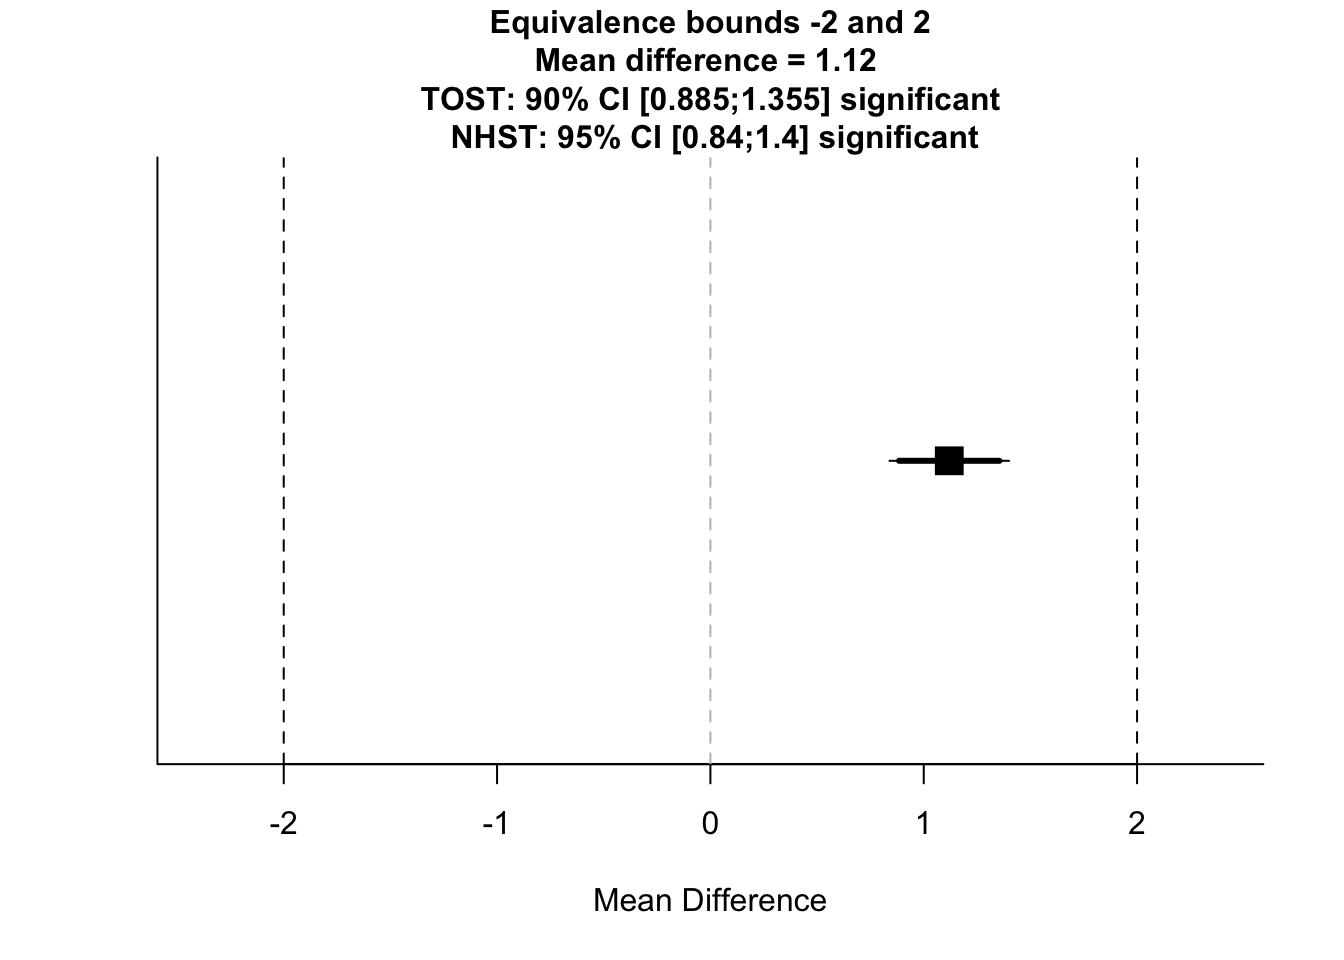
\includegraphics{r4psych_files/figure-latex/10_tost_raw-1.pdf}

Here, we get an output telling us the result of our test in regards to a normal \emph{t}-test (NHST), and under the TOST procedure. We also get reminder of our equivalence bounds, and we get some confidence intervals around our scores. In this case, the normal \emph{t}-test (NHST) was significant, as was the TOST in both directions. This means that although we found a statistically significant difference between the groups, they are statistically equivalent with our criteria. As you can see, differences between groups can be statistically significant, but the effect is so small that we don't care.

\hypertarget{tost-for-effect-sizes}{%
\subsubsection{TOST for Effect Sizes}\label{tost-for-effect-sizes}}

Next, we'll look at a case when we already know the means and standard deviations, but we define our bounds in terms of effect sizes. For this, we only need the \texttt{TOSTtwo()} function. The main difference here is that we specify our bounds in terms of effect sizes (in this case, Cohen's \emph{d}), but everything else remains the same. We'll use a simpler case where we just input some values for the means, standard deviations, and \emph{n}s.

\begin{Shaded}
\begin{Highlighting}[]
\FunctionTok{TOSTtwo}\NormalTok{(}
  \AttributeTok{m1 =} \DecValTok{100}\NormalTok{,}
  \AttributeTok{m2 =} \DecValTok{101}\NormalTok{,}
  \AttributeTok{sd1 =} \DecValTok{9}\NormalTok{,}
  \AttributeTok{sd2 =} \FloatTok{8.1}\NormalTok{,}
  \AttributeTok{n1 =} \DecValTok{192}\NormalTok{,}
  \AttributeTok{n2 =} \DecValTok{191}\NormalTok{,}
  \AttributeTok{low\_eqbound\_d =} \SpecialCharTok{{-}}\FloatTok{0.3}\NormalTok{, }
  \AttributeTok{high\_eqbound\_d =} \FloatTok{0.3}\NormalTok{, }
  \AttributeTok{alpha =} \FloatTok{0.05}\NormalTok{, }
  \AttributeTok{var.equal =} \ConstantTok{FALSE}
\NormalTok{  )}
\end{Highlighting}
\end{Shaded}

\begin{verbatim}
## Note: this function is defunct. Please use tsum_TOST instead
\end{verbatim}

\begin{verbatim}
## TOST results:
## t-value lower bound: 1.79    p-value lower bound: 0.037
## t-value upper bound: -4.08   p-value upper bound: 0.00003
## degrees of freedom : 377.25
## 
## Equivalence bounds (Cohen's d):
## low eqbound: -0.3 
## high eqbound: 0.3
## 
## Equivalence bounds (raw scores):
## low eqbound: -2.5686 
## high eqbound: 2.5686
## 
## TOST confidence interval:
## lower bound 90% CI: -2.443
## upper bound 90% CI:  0.443
## 
## NHST confidence interval:
## lower bound 95% CI: -2.72
## upper bound 95% CI:  0.72
## 
## Equivalence Test Result:
## The equivalence test was significant, t(377.25) = 1.793, p = 0.0369, given equivalence bounds of -2.569 and 2.569 (on a raw scale) and an alpha of 0.05.
\end{verbatim}

\begin{verbatim}
## 
\end{verbatim}

\begin{verbatim}
## 
## Null Hypothesis Test Result:
## The null hypothesis test was non-significant, t(377.25) = -1.143, p = 0.254, given an alpha of 0.05.
\end{verbatim}

\begin{verbatim}
## 
\end{verbatim}

\begin{verbatim}
## NHST: don't reject null significance hypothesis that the effect is equal to 0 
## TOST: reject null equivalence hypothesis
\end{verbatim}

\includegraphics{r4psych_files/figure-latex/10_tost_effect_size-1.pdf}

Here, we can see that the Welch's independent samples \emph{t}-test was non-significant, but the TOST was significant. This means that we didn't find a significant difference between groups and the groups are statistically equivalent.

This pacakge covers TOST for meta-analysis, one- independent- and paired-samples \emph{t}-tests. Check out these functions by typing \texttt{??TOST} in the console. There's a lot more to understanding this procedure than I can cover here, but if you're interested in equivalence tests, you should check out \href{http://journals.sagepub.com/doi/abs/10.1177/1948550617697177}{this primer} by the package author, Daniel Lakens.

Next, we'll cover how we can use R to understand just why we need other open science practices along with the statistics that we calculate and report in R.

\hypertarget{understanding-problematic-design-choices}{%
\section{Understanding Problematic Design Choices}\label{understanding-problematic-design-choices}}

Finally, we'll touch briefly on why you should adopt Open Science practices now that you know how to create reproducible reports. We'll use some simulations to explore cases where you may inadvertantly inflate your error rate through flexible analysis plans. Namely, we'll look at optional stopping; choosing when you should stop recruiting participants on the fly based on your test statistics (and how to avoid inflating your error rate), and why statistics can't save you from poor hypotheses.

\hypertarget{optional-stopping-without-correction}{%
\subsection{Optional Stopping (Without Correction)}\label{optional-stopping-without-correction}}

The real strength in null hypothesis significance testing is that it enables us to make statements about how how often we'll be wrong in the long run (i.e.~to make a type-I error) if we make our inferences based on a certain threshold \emph{p}-value. However, this is only the case if you stick to your research plan from the outset.

Let's look at a case where we can end up fooling ourselves that we have an effect when there isn't a true effect in the population if we change our desgn on the fly. This example is inspired by the section on optional stopping in the \href{https://www.coursera.org/learn/statistical-inferences}{Improving your Statistical Inferences} course by Daniel Lakens.

Here, we'll test our hypothesis that two groups have different IQs (which isn't the case), but if after the first 60 participants we have a non-significant result we'll recruit another 20 and see how this affects our \emph{p}-value distribution.

First, we'll make some functions to (1) sample data and put them in a tibble with a group identifier, (2) run a \emph{t}-test on those groups and capture the \emph{p}-value, and (3) a biased test where we run a \emph{t}-test on our groups, but if it's non-significant, we run additional participants and rerun the \emph{t}-test with the larger sample size.

\begin{Shaded}
\begin{Highlighting}[]
\CommentTok{\# sample data and make a tibble with DV and ID based on input group sample size}
\CommentTok{\# this is fixed at means of 100 and sd of 15 for each group}
\NormalTok{sample\_groups }\OtherTok{\textless{}{-}} \ControlFlowTok{function}\NormalTok{(n\_group)\{}
\NormalTok{  group\_one }\OtherTok{\textless{}{-}} \FunctionTok{rnorm}\NormalTok{(}\AttributeTok{n =}\NormalTok{ n\_group, }\AttributeTok{mean =} \DecValTok{100}\NormalTok{, }\AttributeTok{sd =} \DecValTok{15}\NormalTok{)}
\NormalTok{  group\_two }\OtherTok{\textless{}{-}} \FunctionTok{rnorm}\NormalTok{(}\AttributeTok{n =}\NormalTok{ n\_group, }\AttributeTok{mean =} \DecValTok{100}\NormalTok{, }\AttributeTok{sd =} \DecValTok{15}\NormalTok{)}
\NormalTok{  data }\OtherTok{\textless{}{-}} \FunctionTok{tibble}\NormalTok{(}\AttributeTok{dv =} \FunctionTok{c}\NormalTok{(group\_one, group\_two),}
                 \AttributeTok{id =} \FunctionTok{c}\NormalTok{(}\FunctionTok{rep}\NormalTok{(}\StringTok{"group\_one"}\NormalTok{, n\_group),}
                        \FunctionTok{rep}\NormalTok{(}\StringTok{"group\_two"}\NormalTok{, n\_group)}
\NormalTok{                        )}
\NormalTok{  )}
\NormalTok{\}}

\CommentTok{\# run a t{-}test and extract the p{-}value for a tibble}
\CommentTok{\# columns must be named dv and id for dependent variables and group ID}
\NormalTok{test\_groups }\OtherTok{\textless{}{-}} \ControlFlowTok{function}\NormalTok{(tibble\_data) \{}
\NormalTok{  test }\OtherTok{\textless{}{-}} \FunctionTok{t.test}\NormalTok{(dv }\SpecialCharTok{\textasciitilde{}}\NormalTok{ id, }\AttributeTok{data =}\NormalTok{ tibble\_data, }\AttributeTok{paired =} \ConstantTok{FALSE}\NormalTok{)}
\NormalTok{  test}\SpecialCharTok{$}\NormalTok{p.value}
\NormalTok{\}}

\CommentTok{\# optional stopping without correction:}
\CommentTok{\# sample data and extract p{-}values from a t{-}test}
\CommentTok{\# if non{-}significant, sample additional people and retest}
\NormalTok{bias\_test }\OtherTok{\textless{}{-}} \ControlFlowTok{function}\NormalTok{(sample\_size, additional\_n) \{}
\NormalTok{  original\_data }\OtherTok{\textless{}{-}} \FunctionTok{sample\_groups}\NormalTok{(sample\_size)}
\NormalTok{  p\_val }\OtherTok{\textless{}{-}} \FunctionTok{test\_groups}\NormalTok{(original\_data)}
  \FunctionTok{ifelse}\NormalTok{(p\_val }\SpecialCharTok{\textgreater{}=}\NormalTok{ .}\DecValTok{05}\NormalTok{, }
\NormalTok{         p\_val }\OtherTok{\textless{}{-}} \FunctionTok{test\_groups}\NormalTok{(}
           \FunctionTok{rbind}\NormalTok{(original\_data, }\FunctionTok{sample\_groups}\NormalTok{(additional\_n))}
\NormalTok{           ),}
\NormalTok{         p\_val}
\NormalTok{         )}
\NormalTok{\}}
\end{Highlighting}
\end{Shaded}

Now that we have our functions ready, we can caputre all \emph{p}-values assuming we run the study 1000 times with the idea of testing and getting more participants before re-testing if non-significant.

\begin{Shaded}
\begin{Highlighting}[]
\FunctionTok{set.seed}\NormalTok{(}\DecValTok{100}\NormalTok{) }\CommentTok{\# uncomment if you want different values each time}
\NormalTok{p\_vals }\OtherTok{\textless{}{-}} \FunctionTok{replicate}\NormalTok{(}\AttributeTok{n =} \DecValTok{1000}\NormalTok{, }\FunctionTok{bias\_test}\NormalTok{(}\DecValTok{30}\NormalTok{, }\DecValTok{10}\NormalTok{))}

\CommentTok{\# calculate the proportion of p{-}values below .05}
\FunctionTok{mean}\NormalTok{(p\_vals }\SpecialCharTok{\textless{}} \FloatTok{0.05}\NormalTok{)}
\end{Highlighting}
\end{Shaded}

\begin{verbatim}
## [1] 0.088
\end{verbatim}

What we see is that 8.8\% of our \emph{p}-values are signficant below the .05 \(\alpha\)-level. Really though, this should be 5\% if the null hypothesis is true (which it is). This means that we're inflating our type-I error rate by being so flexible in our testing and analysis procedure. It's easy to fool yourself this way!

Let's have a look at a plot of our \emph{p}-values. You can see that we have many more \emph{p}-values below the .05 threshold. This is despite the fact that \emph{p}-values should be evenly distributed under the null hypothesis.

\begin{Shaded}
\begin{Highlighting}[]
\NormalTok{p\_plot }\OtherTok{\textless{}{-}} \FunctionTok{ggplot}\NormalTok{() }\SpecialCharTok{+} 
  \FunctionTok{geom\_histogram}\NormalTok{(}\FunctionTok{aes}\NormalTok{(p\_vals),}
                 \AttributeTok{binwidth =} \FloatTok{0.05}\NormalTok{,}
                 \AttributeTok{boundary =} \DecValTok{0}\NormalTok{,}
                 \AttributeTok{fill =} \StringTok{"white"}\NormalTok{,}
                 \AttributeTok{colour =} \StringTok{"black"}\NormalTok{) }\SpecialCharTok{+}
  \FunctionTok{scale\_x\_continuous}\NormalTok{(}\AttributeTok{limits =} \FunctionTok{c}\NormalTok{(}\DecValTok{0}\NormalTok{, }\DecValTok{1}\NormalTok{), }
                     \AttributeTok{breaks =} \FunctionTok{seq}\NormalTok{(}\AttributeTok{from =} \DecValTok{0}\NormalTok{, }\AttributeTok{to =} \DecValTok{1}\NormalTok{, }\AttributeTok{by =} \FloatTok{0.05}\NormalTok{)}
\NormalTok{                     ) }\SpecialCharTok{+}
  \FunctionTok{geom\_vline}\NormalTok{(}\AttributeTok{xintercept =} \FloatTok{0.05}\NormalTok{, }\AttributeTok{linetype =} \DecValTok{2}\NormalTok{, }\AttributeTok{colour =} \StringTok{"red"}\NormalTok{) }\SpecialCharTok{+}
  \FunctionTok{labs}\NormalTok{(}\AttributeTok{x =} \StringTok{"p{-}value"}\NormalTok{) }\SpecialCharTok{+}
  \FunctionTok{theme}\NormalTok{(}\AttributeTok{axis.text.x =} \FunctionTok{element\_text}\NormalTok{(}\AttributeTok{size=}\DecValTok{8}\NormalTok{))}
\NormalTok{p\_plot}
\end{Highlighting}
\end{Shaded}

\includegraphics{r4psych_files/figure-latex/10_optional_stopping_plot-1.pdf}

One way to remedy this situation is through optional stopping with a \emph{p}-value correction. If you specify how many times you will look at your data and run a test before deciding whether or not to test more participants, you can correct your \emph{p}-value to account for the infaltion in type-I error rate. One simple way is with the Bonferroni correction. Take your \emph{p}-value, and multiply it by how many times you tested the data. There are less conservative procedures out there, but this is one simple method.

\hypertarget{bad-hypotheses}{%
\subsection{Bad Hypotheses}\label{bad-hypotheses}}

If you have an outlandish hypothesis, where your hypothesis is unlikely to be true, you have a very low chance that a positive result indicates your hypothesis is true. We'll explore an example from the excellent \href{http://xcelab.net/rm/statistical-rethinking/}{Statistical Rethinking} by Richard McElreath to test the truth of this statement. (Honestly, this book has changed how I understand statistics!)

To test this idea this, we can rely on Bayes' theorem. I won't show you the ins and outs of this theorem, but just know that the function that allows you to change the power of your study, your alpha level, and the probability that your hypothesis is true. The default values make sure that you have a design with 90\% power and a 5\% \(\alpha\)-level, assuming that your hypothesis only has a 1\% chance of being true.

\begin{Shaded}
\begin{Highlighting}[]
\NormalTok{test\_prob\_hyp\_true }\OtherTok{\textless{}{-}} \ControlFlowTok{function}\NormalTok{(}\AttributeTok{power =} \FloatTok{0.90}\NormalTok{, }\AttributeTok{alpha =} \FloatTok{0.05}\NormalTok{, }\AttributeTok{hyp\_chance =} \FloatTok{0.01}\NormalTok{)\{}
  \CommentTok{\# calculate probabilities}
\NormalTok{  prob\_false }\OtherTok{\textless{}{-}} \DecValTok{1} \SpecialCharTok{{-}}\NormalTok{ hyp\_chance}
\NormalTok{  prob\_positive }\OtherTok{\textless{}{-}}\NormalTok{ power }\SpecialCharTok{*}\NormalTok{ hyp\_chance }\SpecialCharTok{+}\NormalTok{ alpha }\SpecialCharTok{*}\NormalTok{ prob\_false}
\NormalTok{  prob\_positive\_is\_true }\OtherTok{\textless{}{-}}\NormalTok{ power }\SpecialCharTok{*}\NormalTok{ hyp\_chance }\SpecialCharTok{/}\NormalTok{ prob\_positive}
  
  \CommentTok{\# output probability of a positive result being true}
  \FunctionTok{print}\NormalTok{(}\FunctionTok{paste}\NormalTok{(}\StringTok{"There is a"}\NormalTok{, }
              \FunctionTok{round}\NormalTok{(prob\_positive\_is\_true}\SpecialCharTok{*}\DecValTok{100}\NormalTok{, }\DecValTok{2}\NormalTok{), }
              \StringTok{"\% chance of a positive result being true."}\NormalTok{)}
\NormalTok{  )}
\NormalTok{\}}
\end{Highlighting}
\end{Shaded}

We'll test the probability of a positive result being true under these default assumptions.

\begin{Shaded}
\begin{Highlighting}[]
\FunctionTok{test\_prob\_hyp\_true}\NormalTok{()}
\end{Highlighting}
\end{Shaded}

\begin{verbatim}
## [1] "There is a 15.38 % chance of a positive result being true."
\end{verbatim}

But what if we change the probability of the hypothesis being true to even 25\%?

\begin{Shaded}
\begin{Highlighting}[]
\FunctionTok{test\_prob\_hyp\_true}\NormalTok{(}\AttributeTok{hyp\_chance =} \FloatTok{0.25}\NormalTok{)}
\end{Highlighting}
\end{Shaded}

\begin{verbatim}
## [1] "There is a 85.71 % chance of a positive result being true."
\end{verbatim}

Even with only a \(\frac{1}{4}\) chance of our hypothesis being true, we can now more confidently accept a positive result as being positive. The take home message here is that even if you design and test your studies to your best abilities, with very high power, positive findings based on bad hypotheses are likely to be misleading; good statistics can't save you from bad hypotheses.

\hypertarget{the-final-lesson}{%
\section{The Final Lesson}\label{the-final-lesson}}

Congratulations, you've made it! Now watch this video and follow Jeff's advice.

If you ever get stuck with anything, these two book covers always help me.

\textless img src=``..img/Cat.jpg''; style=``max-width:350px''; align=``left''\textgreater{}
\textless img src=``..img/Frog.jpg''; style=``max-width:350px''; align=``right\textgreater{}

\hypertarget{exercises-9}{%
\section{Exercises}\label{exercises-9}}

For these exercises, we will look at the core concepts from this lesson. As always, load the libraries necessary for this lesson.

\begin{Shaded}
\begin{Highlighting}[]
\FunctionTok{library}\NormalTok{(tidyverse)}
\FunctionTok{library}\NormalTok{(effsize)}
\FunctionTok{library}\NormalTok{(TOSTER)}
\end{Highlighting}
\end{Shaded}

For this exercise, we'll look at doing a full analysis using a data set and report from the excellent \href{https://sites.trinity.edu/osl}{Open Stats Lab}. For simplicity, we'll load this data directly from a csv file stored on GitHub. (To get a link for this, you must view the raw file on GitHub online.)

Schroeder and Epley(2015) explored whether you'd be more likely to get a new job after delivering a speech describing your skills, or if you wrote a speech and had a potential employer read it out.

Prediction: A person's speech (i.e., vocal tone, cadence, and pitch) communicates information about intelligence better than written words.
Participants: 39 professional recruiters in one of two conditions.
Conditions: Listen to audio recording of speech, or read speech aloud.
Dependent Variable: Intellect aggregated across intelligence, competence, and thoughtfulness.

Also rated overall impression (composite of positive and negative), and how likely they would be to hire them (0 = not at all, 10 = extremely likely).

\begin{Shaded}
\begin{Highlighting}[]
\CommentTok{\# read in the data}
\NormalTok{raw\_data }\OtherTok{\textless{}{-}} \FunctionTok{read\_csv}\NormalTok{(}
  \StringTok{"https://raw.githubusercontent.com/gpwilliams/r4psych/master/lesson\_materials/10\_reporting\_reproducible\_research/inputs/schroeder\_epley\_2015.csv"}
\NormalTok{  )}
\end{Highlighting}
\end{Shaded}

\hypertarget{question-1-9}{%
\subsection{Question 1}\label{question-1-9}}

Subset the data to the columns relevant to the research question, and make the names all lowercase for consistency. Call this, \texttt{data\_subset}.

\hypertarget{question-2-9}{%
\subsection{Question 2}\label{question-2-9}}

Summarise the data, creating means, standard deviations, and ns for each group in the data set. Call this \texttt{data\_summary}. Put the summary in a table using the \texttt{kable()} command.

\hypertarget{question-3-9}{%
\subsection{Question 3}\label{question-3-9}}

Create a plot to display the differences across the groups.

\hypertarget{question-4-9}{%
\subsection{Question 4}\label{question-4-9}}

Test the assumptions of an independent-samples \emph{t}-test.

\hypertarget{question-5-9}{%
\subsection{Question 5}\label{question-5-9}}

Assuming the test assumptions are met, fit a model to your data, save this as \texttt{t\_test\_output}. For this case, we will just look at the effect of Intellect. Output the test on completion. (Note: do not use \texttt{summary()} here, instead just type the name of the object.)

\hypertarget{question-6-9}{%
\subsection{Question 6}\label{question-6-9}}

Calculate effect sizes for the \emph{t}-test. The choice of effect size is up to you.

\hypertarget{question-7-8}{%
\subsection{Question 7}\label{question-7-8}}

Perform a TOST on your data evaluating the equivalence against a lower bound of -0.5 and upper bound of 0.5. What does this tell us? (Hint: Use the \texttt{with()} function on the data\_summary object to access the columns for that data source.)

\hypertarget{question-8-7}{%
\subsection{Question 8}\label{question-8-7}}

A. Fit a linear model to the data. Save this as \texttt{lm\_test\_output}. How does this compare with the \emph{t}-test?
B. Output 95\% confidence intervals for the linear model. Why do they differ to that of the \emph{t}-test?

  \bibliography{references.bib,packages.bib}

\end{document}
